\documentclass[twoside]{book}

% Packages required by doxygen
\usepackage{fixltx2e}
\usepackage{calc}
\usepackage{doxygen}
\usepackage[export]{adjustbox} % also loads graphicx
\usepackage{graphicx}
\usepackage[utf8]{inputenc}
\usepackage{makeidx}
\usepackage{multicol}
\usepackage{multirow}
\PassOptionsToPackage{warn}{textcomp}
\usepackage{textcomp}
\usepackage[nointegrals]{wasysym}
\usepackage[table]{xcolor}

% Font selection
\usepackage[T1]{fontenc}
\usepackage[scaled=.90]{helvet}
\usepackage{courier}
\usepackage{amssymb}
\usepackage{sectsty}
\renewcommand{\familydefault}{\sfdefault}
\allsectionsfont{%
  \fontseries{bc}\selectfont%
  \color{darkgray}%
}
\renewcommand{\DoxyLabelFont}{%
  \fontseries{bc}\selectfont%
  \color{darkgray}%
}
\newcommand{\+}{\discretionary{\mbox{\scriptsize$\hookleftarrow$}}{}{}}

% Page & text layout
\usepackage{geometry}
\geometry{%
  a4paper,%
  top=2.5cm,%
  bottom=2.5cm,%
  left=2.5cm,%
  right=2.5cm%
}
\tolerance=750
\hfuzz=15pt
\hbadness=750
\setlength{\emergencystretch}{15pt}
\setlength{\parindent}{0cm}
\setlength{\parskip}{3ex plus 2ex minus 2ex}
\makeatletter
\renewcommand{\paragraph}{%
  \@startsection{paragraph}{4}{0ex}{-1.0ex}{1.0ex}{%
    \normalfont\normalsize\bfseries\SS@parafont%
  }%
}
\renewcommand{\subparagraph}{%
  \@startsection{subparagraph}{5}{0ex}{-1.0ex}{1.0ex}{%
    \normalfont\normalsize\bfseries\SS@subparafont%
  }%
}
\makeatother

% Headers & footers
\usepackage{fancyhdr}
\pagestyle{fancyplain}
\fancyhead[LE]{\fancyplain{}{\bfseries\thepage}}
\fancyhead[CE]{\fancyplain{}{}}
\fancyhead[RE]{\fancyplain{}{\bfseries\leftmark}}
\fancyhead[LO]{\fancyplain{}{\bfseries\rightmark}}
\fancyhead[CO]{\fancyplain{}{}}
\fancyhead[RO]{\fancyplain{}{\bfseries\thepage}}
\fancyfoot[LE]{\fancyplain{}{}}
\fancyfoot[CE]{\fancyplain{}{}}
\fancyfoot[RE]{\fancyplain{}{\bfseries\scriptsize Generated by Doxygen }}
\fancyfoot[LO]{\fancyplain{}{\bfseries\scriptsize Generated by Doxygen }}
\fancyfoot[CO]{\fancyplain{}{}}
\fancyfoot[RO]{\fancyplain{}{}}
\renewcommand{\footrulewidth}{0.4pt}
\renewcommand{\chaptermark}[1]{%
  \markboth{#1}{}%
}
\renewcommand{\sectionmark}[1]{%
  \markright{\thesection\ #1}%
}

% Indices & bibliography
\usepackage{natbib}
\usepackage[titles]{tocloft}
\setcounter{tocdepth}{3}
\setcounter{secnumdepth}{5}
\makeindex

% Hyperlinks (required, but should be loaded last)
\usepackage{ifpdf}
\ifpdf
  \usepackage[pdftex,pagebackref=true]{hyperref}
\else
  \usepackage[ps2pdf,pagebackref=true]{hyperref}
\fi
\hypersetup{%
  colorlinks=true,%
  linkcolor=blue,%
  citecolor=blue,%
  unicode%
}

% Custom commands
\newcommand{\clearemptydoublepage}{%
  \newpage{\pagestyle{empty}\cleardoublepage}%
}

\usepackage{caption}
\captionsetup{labelsep=space,justification=centering,font={bf},singlelinecheck=off,skip=4pt,position=top}

%===== C O N T E N T S =====

\begin{document}

% Titlepage & ToC
\hypersetup{pageanchor=false,
             bookmarksnumbered=true,
             pdfencoding=unicode
            }
\pagenumbering{alph}
\begin{titlepage}
\vspace*{7cm}
\begin{center}%
{\Large Embedded Element Method Algorithms (E\+M\+MA) }\\
\vspace*{1cm}
{\large Generated by Doxygen 1.8.13}\\
\end{center}
\end{titlepage}
\clearemptydoublepage
\pagenumbering{roman}
\tableofcontents
\clearemptydoublepage
\pagenumbering{arabic}
\hypersetup{pageanchor=true}

%--- Begin generated contents ---
\chapter{Main Page}
\label{index}\hypertarget{index}{}\subsection*{To install using C\+Make\+:}

1. cd embeddedfem

2. mkdir build

3. cd build

4. ccmake ..

5. make

\subsection*{How to run the code\+:}

1. you need to compile with examples ON in the cmake configuration (step 4 above)

2. navigate to $\sim$/embeddedfem/build/examples/example-\/1

3. ./example1 . input.\+inp

\href{http://www.mne.psu.edu/compbio}{\tt P\+SU Comp Bio Group}  
\chapter{Class Index}
\section{Class List}
Here are the classes, structs, unions and interfaces with brief descriptions\+:\begin{DoxyCompactList}
\item\contentsline{section}{\hyperlink{class_b_c}{BC} }{\pageref{class_b_c}}{}
\item\contentsline{section}{\hyperlink{class_materials}{Materials} }{\pageref{class_materials}}{}
\item\contentsline{section}{\hyperlink{class_mesh}{Mesh} }{\pageref{class_mesh}}{}
\end{DoxyCompactList}

\chapter{File Index}
\section{File List}
Here is a list of all files with brief descriptions\+:\begin{DoxyCompactList}
\item\contentsline{section}{src/eema/examples/example-\/1/\hyperlink{main_8cpp}{main.\+cpp} }{\pageref{main_8cpp}}{}
\item\contentsline{section}{src/eema/include/\hyperlink{_b_c_8h}{B\+C.\+h} }{\pageref{_b_c_8h}}{}
\item\contentsline{section}{src/eema/include/\hyperlink{functions_8h}{functions.\+h} }{\pageref{functions_8h}}{}
\item\contentsline{section}{src/eema/include/\hyperlink{_global_variables_8h}{Global\+Variables.\+h} }{\pageref{_global_variables_8h}}{}
\item\contentsline{section}{src/eema/include/\hyperlink{_materials_8h}{Materials.\+h} }{\pageref{_materials_8h}}{}
\item\contentsline{section}{src/eema/include/\hyperlink{_mesh_8h}{Mesh.\+h} }{\pageref{_mesh_8h}}{}
\item\contentsline{section}{src/eema/src/\+Elements/\+Element\+Calculations/\hyperlink{fe__cal_def_grad_8cpp}{fe\+\_\+cal\+Def\+Grad.\+cpp} }{\pageref{fe__cal_def_grad_8cpp}}{}
\item\contentsline{section}{src/eema/src/\+Elements/\+Element\+Calculations/\hyperlink{fe__cal_jacobian_8cpp}{fe\+\_\+cal\+Jacobian.\+cpp} }{\pageref{fe__cal_jacobian_8cpp}}{}
\item\contentsline{section}{src/eema/src/\+Elements/\+Element\+Calculations/\hyperlink{fe__cal_simp_transformation_8cpp}{fe\+\_\+cal\+Simp\+Transformation.\+cpp} }{\pageref{fe__cal_simp_transformation_8cpp}}{}
\item\contentsline{section}{src/eema/src/\+Elements/\+Element\+Calculations/\hyperlink{fe__cal_transformation_8cpp}{fe\+\_\+cal\+Transformation.\+cpp} }{\pageref{fe__cal_transformation_8cpp}}{}
\item\contentsline{section}{src/eema/src/\+Elements/\+Element\+Calculations/\hyperlink{fe__max_element_length_8cpp}{fe\+\_\+max\+Element\+Length.\+cpp} }{\pageref{fe__max_element_length_8cpp}}{}
\item\contentsline{section}{src/eema/src/\+Elements/\+Element\+Calculations/\hyperlink{fe__min_element_length_8cpp}{fe\+\_\+min\+Element\+Length.\+cpp} }{\pageref{fe__min_element_length_8cpp}}{}
\item\contentsline{section}{src/eema/src/\+Elements/\+Element\+Calculations/\hyperlink{fe__str_disp_matrix_8cpp}{fe\+\_\+str\+Disp\+Matrix.\+cpp} }{\pageref{fe__str_disp_matrix_8cpp}}{}
\item\contentsline{section}{src/eema/src/\+Elements/\+Element\+Calculations/\hyperlink{fe__tensor2voigt_8cpp}{fe\+\_\+tensor2voigt.\+cpp} }{\pageref{fe__tensor2voigt_8cpp}}{}
\item\contentsline{section}{src/eema/src/\+Elements/\+Element\+Calculations/\hyperlink{fe__transform_mass_8cpp}{fe\+\_\+transform\+Mass.\+cpp} }{\pageref{fe__transform_mass_8cpp}}{}
\item\contentsline{section}{src/eema/src/\+Elements/\+Element\+Calculations/\hyperlink{fe__voigt2tensor_8cpp}{fe\+\_\+voigt2tensor.\+cpp} }{\pageref{fe__voigt2tensor_8cpp}}{}
\item\contentsline{section}{src/eema/src/\+Elements/\+Internal\+Nodal\+Force/\hyperlink{fe__stiffness__embed__truss_8cpp}{fe\+\_\+stiffness\+\_\+embed\+\_\+truss.\+cpp} }{\pageref{fe__stiffness__embed__truss_8cpp}}{}
\item\contentsline{section}{src/eema/src/\+Elements/\+Internal\+Nodal\+Force/\hyperlink{fe__stiffness__hex_8cpp}{fe\+\_\+stiffness\+\_\+hex.\+cpp} }{\pageref{fe__stiffness__hex_8cpp}}{}
\item\contentsline{section}{src/eema/src/\+Elements/\+Mass/\hyperlink{fe__mass__hex_8cpp}{fe\+\_\+mass\+\_\+hex.\+cpp} }{\pageref{fe__mass__hex_8cpp}}{}
\item\contentsline{section}{src/eema/src/\+Elements/\+Mass/\hyperlink{fe__mass_lumped_8cpp}{fe\+\_\+mass\+Lumped.\+cpp} }{\pageref{fe__mass_lumped_8cpp}}{}
\item\contentsline{section}{src/eema/src/\+Elements/\+Quadrature/\hyperlink{fe__guass__points_8cpp}{fe\+\_\+guass\+\_\+points.\+cpp} }{\pageref{fe__guass__points_8cpp}}{}
\item\contentsline{section}{src/eema/src/\+Elements/\+Quadrature/\hyperlink{fe__guass__points__3d_8cpp}{fe\+\_\+guass\+\_\+points\+\_\+3d.\+cpp} }{\pageref{fe__guass__points__3d_8cpp}}{}
\item\contentsline{section}{src/eema/src/\+Elements/\+Quadrature/\hyperlink{fe__guass__weights_8cpp}{fe\+\_\+guass\+\_\+weights.\+cpp} }{\pageref{fe__guass__weights_8cpp}}{}
\item\contentsline{section}{src/eema/src/\+Elements/\+Quadrature/\hyperlink{fe__guass__weights__3d_8cpp}{fe\+\_\+guass\+\_\+weights\+\_\+3d.\+cpp} }{\pageref{fe__guass__weights__3d_8cpp}}{}
\item\contentsline{section}{src/eema/src/\+Elements/\+Shape\+Functions/\hyperlink{fe__dn__actual__8_8cpp}{fe\+\_\+dn\+\_\+actual\+\_\+8.\+cpp} }{\pageref{fe__dn__actual__8_8cpp}}{}
\item\contentsline{section}{src/eema/src/\+Elements/\+Shape\+Functions/\hyperlink{fe__dn__iso__8_8cpp}{fe\+\_\+dn\+\_\+iso\+\_\+8.\+cpp} }{\pageref{fe__dn__iso__8_8cpp}}{}
\item\contentsline{section}{src/eema/src/\+Elements/\+Shape\+Functions/\hyperlink{fe__shape_matrix_8cpp}{fe\+\_\+shape\+Matrix.\+cpp} }{\pageref{fe__shape_matrix_8cpp}}{}
\item\contentsline{section}{src/eema/src/\+Elements/\+Shape\+Functions/\hyperlink{fe__shapes_8cpp}{fe\+\_\+shapes.\+cpp} }{\pageref{fe__shapes_8cpp}}{}
\item\contentsline{section}{src/eema/src/\+F\+E\+M/\+Assembly-\/\+Global-\/\+Local/\hyperlink{fe__assemble__mass_8cpp}{fe\+\_\+assemble\+\_\+mass.\+cpp} }{\pageref{fe__assemble__mass_8cpp}}{}
\item\contentsline{section}{src/eema/src/\+F\+E\+M/\+Assembly-\/\+Global-\/\+Local/\hyperlink{fe__find__index_8cpp}{fe\+\_\+find\+\_\+index.\+cpp} }{\pageref{fe__find__index_8cpp}}{}
\item\contentsline{section}{src/eema/src/\+F\+E\+M/\+Assembly-\/\+Global-\/\+Local/\hyperlink{fe__gather_8cpp}{fe\+\_\+gather.\+cpp} }{\pageref{fe__gather_8cpp}}{}
\item\contentsline{section}{src/eema/src/\+F\+E\+M/\+Assembly-\/\+Global-\/\+Local/\hyperlink{fe__scatter_8cpp}{fe\+\_\+scatter.\+cpp} }{\pageref{fe__scatter_8cpp}}{}
\item\contentsline{section}{src/eema/src/\+F\+E\+M/\+Boundary\+Conditions/\hyperlink{fe__apply__bc_8cpp}{fe\+\_\+apply\+\_\+bc.\+cpp} }{\pageref{fe__apply__bc_8cpp}}{}
\item\contentsline{section}{src/eema/src/\+F\+E\+M/\+Constraints/\+Embedded\+Element/\hyperlink{fe__compute__host_8cpp}{fe\+\_\+compute\+\_\+host.\+cpp} }{\pageref{fe__compute__host_8cpp}}{}
\item\contentsline{section}{src/eema/src/\+F\+E\+M/\+Constraints/\+Embedded\+Element/\hyperlink{fe__create__bbox_8cpp}{fe\+\_\+create\+\_\+bbox.\+cpp} }{\pageref{fe__create__bbox_8cpp}}{}
\item\contentsline{section}{src/eema/src/\+F\+E\+M/\+Constraints/\+Embedded\+Element/\hyperlink{fe__embed__preprocessing_8cpp}{fe\+\_\+embed\+\_\+preprocessing.\+cpp} }{\pageref{fe__embed__preprocessing_8cpp}}{}
\item\contentsline{section}{src/eema/src/\+F\+E\+M/\+Constraints/\+Embedded\+Element/\hyperlink{fe__embed__preprocessing__mapping_8cpp}{fe\+\_\+embed\+\_\+preprocessing\+\_\+mapping.\+cpp} }{\pageref{fe__embed__preprocessing__mapping_8cpp}}{}
\item\contentsline{section}{src/eema/src/\+F\+E\+M/\+Electromechanics/\hyperlink{fe__electromechanics_8cpp}{fe\+\_\+electromechanics.\+cpp} }{\pageref{fe__electromechanics_8cpp}}{}
\item\contentsline{section}{src/eema/src/\+F\+E\+M/\+Explicit/\hyperlink{fe__main_e_x_p_l_i_c_i_t_8cpp}{fe\+\_\+main\+E\+X\+P\+L\+I\+C\+I\+T.\+cpp} }{\pageref{fe__main_e_x_p_l_i_c_i_t_8cpp}}{}
\item\contentsline{section}{src/eema/src/\+F\+E\+M/\+Solid\+Mechanics/\hyperlink{fe__calculate_accln_8cpp}{fe\+\_\+calculate\+Accln.\+cpp} }{\pageref{fe__calculate_accln_8cpp}}{}
\item\contentsline{section}{src/eema/src/\+F\+E\+M/\+Solid\+Mechanics/\hyperlink{fe__calculate_k_e_8cpp}{fe\+\_\+calculate\+K\+E.\+cpp} }{\pageref{fe__calculate_k_e_8cpp}}{}
\item\contentsline{section}{src/eema/src/\+F\+E\+M/\+Solid\+Mechanics/\hyperlink{fe__calculate_mass_8cpp}{fe\+\_\+calculate\+Mass.\+cpp} }{\pageref{fe__calculate_mass_8cpp}}{}
\item\contentsline{section}{src/eema/src/\+F\+E\+M/\+Solid\+Mechanics/\hyperlink{fe__getforce_8cpp}{fe\+\_\+getforce.\+cpp} }{\pageref{fe__getforce_8cpp}}{}
\item\contentsline{section}{src/eema/src/\+F\+E\+M/\+Solid\+Mechanics/\hyperlink{fe__update_8cpp}{fe\+\_\+update.\+cpp} }{\pageref{fe__update_8cpp}}{}
\item\contentsline{section}{src/eema/src/\+Input-\/\+Output/\+Input/\hyperlink{_b_c_8cpp}{B\+C.\+cpp} }{\pageref{_b_c_8cpp}}{}
\item\contentsline{section}{src/eema/src/\+Input-\/\+Output/\+Input/\hyperlink{fe__main_read_8cpp}{fe\+\_\+main\+Read.\+cpp} }{\pageref{fe__main_read_8cpp}}{}
\item\contentsline{section}{src/eema/src/\+Input-\/\+Output/\+Input/\hyperlink{fe__text2matrix_8cpp}{fe\+\_\+text2matrix.\+cpp} }{\pageref{fe__text2matrix_8cpp}}{}
\item\contentsline{section}{src/eema/src/\+Input-\/\+Output/\+Input/\hyperlink{_materials_8cpp}{Materials.\+cpp} }{\pageref{_materials_8cpp}}{}
\item\contentsline{section}{src/eema/src/\+Input-\/\+Output/\+Input/\hyperlink{_mesh_8cpp}{Mesh.\+cpp} }{\pageref{_mesh_8cpp}}{}
\item\contentsline{section}{src/eema/src/\+Input-\/\+Output/\+Output/\hyperlink{fe__display_8cpp}{fe\+\_\+display.\+cpp} }{\pageref{fe__display_8cpp}}{}
\item\contentsline{section}{src/eema/src/\+Input-\/\+Output/\+Output/\hyperlink{fe__matrix2text_8cpp}{fe\+\_\+matrix2text.\+cpp} }{\pageref{fe__matrix2text_8cpp}}{}
\item\contentsline{section}{src/eema/src/\+Input-\/\+Output/\+Output/\hyperlink{fe__simulation_time_8cpp}{fe\+\_\+simulation\+Time.\+cpp} }{\pageref{fe__simulation_time_8cpp}}{}
\item\contentsline{section}{src/eema/src/\+Input-\/\+Output/\+Output/\hyperlink{fe__vector2text_8cpp}{fe\+\_\+vector2text.\+cpp} }{\pageref{fe__vector2text_8cpp}}{}
\item\contentsline{section}{src/eema/src/\+Input-\/\+Output/\+Output/\hyperlink{fe__vtk_8cpp}{fe\+\_\+vtk.\+cpp} }{\pageref{fe__vtk_8cpp}}{}
\item\contentsline{section}{src/eema/src/\+Input-\/\+Output/\+Output/\hyperlink{fe__vtu_8cpp}{fe\+\_\+vtu.\+cpp} }{\pageref{fe__vtu_8cpp}}{}
\item\contentsline{section}{src/eema/src/\+Input-\/\+Output/\+Output/\hyperlink{fe__write_8cpp}{fe\+\_\+write.\+cpp} }{\pageref{fe__write_8cpp}}{}
\item\contentsline{section}{src/eema/src/\+Materials/\hyperlink{fe__get__mats_8cpp}{fe\+\_\+get\+\_\+mats.\+cpp} }{\pageref{fe__get__mats_8cpp}}{}
\item\contentsline{section}{src/eema/src/\+Materials/\hyperlink{fe__get__model_8cpp}{fe\+\_\+get\+\_\+model.\+cpp} }{\pageref{fe__get__model_8cpp}}{}
\item\contentsline{section}{src/eema/src/\+Materials/\+Elastic/\hyperlink{fe__simple__elastic_8cpp}{fe\+\_\+simple\+\_\+elastic.\+cpp} }{\pageref{fe__simple__elastic_8cpp}}{}
\item\contentsline{section}{src/eema/src/\+Materials/\+Mooney-\/\+Rivlin-\/\+Hyperelastic/\hyperlink{fe__mooneyrivlin__hyperelastic_8cpp}{fe\+\_\+mooneyrivlin\+\_\+hyperelastic.\+cpp} }{\pageref{fe__mooneyrivlin__hyperelastic_8cpp}}{}
\item\contentsline{section}{src/eema/src/\+Materials/\+Ogden-\/\+Hyperelastic/\hyperlink{fe__ogden__hyperelastic_8cpp}{fe\+\_\+ogden\+\_\+hyperelastic.\+cpp} }{\pageref{fe__ogden__hyperelastic_8cpp}}{}
\item\contentsline{section}{src/eema/src/\+Materials/\+Saint-\/\+Venant/\hyperlink{fe__saintvenant__elastic_8cpp}{fe\+\_\+saintvenant\+\_\+elastic.\+cpp} }{\pageref{fe__saintvenant__elastic_8cpp}}{}
\item\contentsline{section}{src/eema/src/\+Materials/\+Stress\+Update/\hyperlink{fe__stress_update_8cpp}{fe\+\_\+stress\+Update.\+cpp} }{\pageref{fe__stress_update_8cpp}}{}
\item\contentsline{section}{src/eema/src/\+Materials/\+Stress\+Update/\hyperlink{fe__stress_update__1d_8cpp}{fe\+\_\+stress\+Update\+\_\+1d.\+cpp} }{\pageref{fe__stress_update__1d_8cpp}}{}
\item\contentsline{section}{src/eema/src/\+Math/\+General\+Math/\hyperlink{fe__cal_area__4_8cpp}{fe\+\_\+cal\+Area\+\_\+4.\+cpp} }{\pageref{fe__cal_area__4_8cpp}}{}
\item\contentsline{section}{src/eema/src/\+Math/\+General\+Math/\hyperlink{fe__cal_volume_8cpp}{fe\+\_\+cal\+Volume.\+cpp} }{\pageref{fe__cal_volume_8cpp}}{}
\item\contentsline{section}{src/eema/src/\+Math/\+General\+Math/\hyperlink{fe__concatenate__vector2matrix_8cpp}{fe\+\_\+concatenate\+\_\+vector2matrix.\+cpp} }{\pageref{fe__concatenate__vector2matrix_8cpp}}{}
\item\contentsline{section}{src/eema/src/\+Math/\+General\+Math/\hyperlink{fe__det_matrix_8cpp}{fe\+\_\+det\+Matrix.\+cpp} }{\pageref{fe__det_matrix_8cpp}}{}
\item\contentsline{section}{src/eema/src/\+Math/\+General\+Math/\hyperlink{fe__find_8cpp}{fe\+\_\+find.\+cpp} }{\pageref{fe__find_8cpp}}{}
\item\contentsline{section}{src/eema/src/\+Math/\+General\+Math/\hyperlink{fe__function_8cpp}{fe\+\_\+function.\+cpp} }{\pageref{fe__function_8cpp}}{}
\item\contentsline{section}{src/eema/src/\+Math/\+General\+Math/\hyperlink{fe__inv_matrix_8cpp}{fe\+\_\+inv\+Matrix.\+cpp} }{\pageref{fe__inv_matrix_8cpp}}{}
\item\contentsline{section}{src/eema/src/\+Math/\+General\+Math/\hyperlink{fe__newton_rhapson_8cpp}{fe\+\_\+newton\+Rhapson.\+cpp} }{\pageref{fe__newton_rhapson_8cpp}}{}
\item\contentsline{section}{src/eema/src/\+Time\+Step/\hyperlink{fe__cal_time_step_8cpp}{fe\+\_\+cal\+Time\+Step.\+cpp} }{\pageref{fe__cal_time_step_8cpp}}{}
\item\contentsline{section}{src/eema/src/\+Time\+Step/\hyperlink{fe__cal_wave_speed_8cpp}{fe\+\_\+cal\+Wave\+Speed.\+cpp} }{\pageref{fe__cal_wave_speed_8cpp}}{}
\item\contentsline{section}{src/eema/src/\+Time\+Step/\hyperlink{fe__get_time_step_8cpp}{fe\+\_\+get\+Time\+Step.\+cpp} }{\pageref{fe__get_time_step_8cpp}}{}
\end{DoxyCompactList}

\chapter{Class Documentation}
\hypertarget{class_b_c}{}\section{BC Class Reference}
\label{class_b_c}\index{BC@{BC}}


{\ttfamily \#include $<$src/eema/include/\+B\+C.\+h$>$}

\subsection*{Public Member Functions}
\begin{DoxyCompactItemize}
\item 
void \hyperlink{class_b_c_a8ceaa781f98b4128fa50611ff9481e1a}{read\+BC} (std\+::string type\+\_\+user, double input\+\_\+amp\+\_\+user, int num\+\_\+dof\+\_\+user, Vector\+Xi dof\+\_\+user, std\+::string time\+\_\+curve\+\_\+user)
\item 
std\+::string \hyperlink{class_b_c_aa6afb3d4586f395578bef89c77e60449}{get\+Type} ()
\item 
double \hyperlink{class_b_c_ad648545e6ee046075350cd9b3c88e610}{get\+Amplitude} ()
\item 
int \hyperlink{class_b_c_a6e42c3db5c67435bf2616768959866e9}{get\+Num\+D\+OF} ()
\item 
Vector\+Xi \hyperlink{class_b_c_a0bc8eb90956a082ada5e4daa5e32c9fc}{get\+D\+OF} ()
\item 
std\+::string \hyperlink{class_b_c_a3590d0a29a9261d99f21ee75340e5722}{get\+Time\+Behavior} ()
\item 
void \hyperlink{class_b_c_a7f2fb6f9d3848e8f0617902b3fb804af}{print\+B\+C\+Info} ()
\end{DoxyCompactItemize}
\subsection*{Private Attributes}
\begin{DoxyCompactItemize}
\item 
std\+::string \hyperlink{class_b_c_ab25297125dceec52f445a3a5efa77784}{type}
\item 
double \hyperlink{class_b_c_a25d7def8fdf5e988602759608b1507ea}{amplitude}
\item 
int \hyperlink{class_b_c_a71fe2e36793286c4e683a3d8485abaf2}{num\+\_\+dof}
\item 
Vector\+Xi \hyperlink{class_b_c_a4e53c8862da8b017b419b201911d9e00}{dof}
\item 
std\+::string \hyperlink{class_b_c_a84f989feaa5e81214f17b6dbdd1cf2ab}{time\+\_\+curve}
\end{DoxyCompactItemize}


\subsection{Detailed Description}


Definition at line \hyperlink{_b_c_8h_source_l00016}{16} of file \hyperlink{_b_c_8h_source}{B\+C.\+h}.



\subsection{Member Function Documentation}
\mbox{\Hypertarget{class_b_c_ad648545e6ee046075350cd9b3c88e610}\label{class_b_c_ad648545e6ee046075350cd9b3c88e610}} 
\index{BC@{BC}!get\+Amplitude@{get\+Amplitude}}
\index{get\+Amplitude@{get\+Amplitude}!BC@{BC}}
\subsubsection{\texorpdfstring{get\+Amplitude()}{getAmplitude()}}
{\footnotesize\ttfamily double B\+C\+::get\+Amplitude (\begin{DoxyParamCaption}{ }\end{DoxyParamCaption})}



Definition at line \hyperlink{_b_c_8cpp_source_l00018}{18} of file \hyperlink{_b_c_8cpp_source}{B\+C.\+cpp}.

Here is the caller graph for this function\+:\nopagebreak
\begin{figure}[H]
\begin{center}
\leavevmode
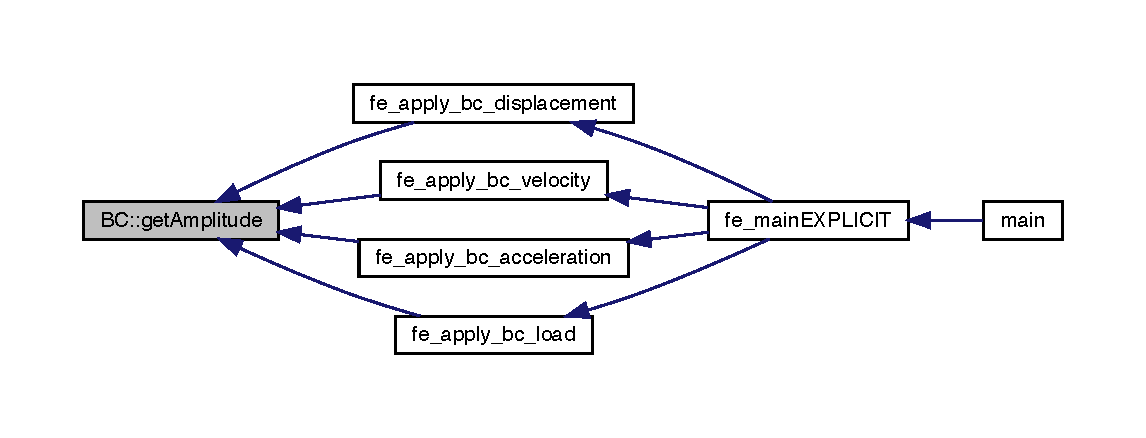
\includegraphics[width=350pt]{class_b_c_ad648545e6ee046075350cd9b3c88e610_icgraph}
\end{center}
\end{figure}
\mbox{\Hypertarget{class_b_c_a0bc8eb90956a082ada5e4daa5e32c9fc}\label{class_b_c_a0bc8eb90956a082ada5e4daa5e32c9fc}} 
\index{BC@{BC}!get\+D\+OF@{get\+D\+OF}}
\index{get\+D\+OF@{get\+D\+OF}!BC@{BC}}
\subsubsection{\texorpdfstring{get\+D\+O\+F()}{getDOF()}}
{\footnotesize\ttfamily Vector\+Xi B\+C\+::get\+D\+OF (\begin{DoxyParamCaption}{ }\end{DoxyParamCaption})}



Definition at line \hyperlink{_b_c_8cpp_source_l00026}{26} of file \hyperlink{_b_c_8cpp_source}{B\+C.\+cpp}.

Here is the caller graph for this function\+:\nopagebreak
\begin{figure}[H]
\begin{center}
\leavevmode
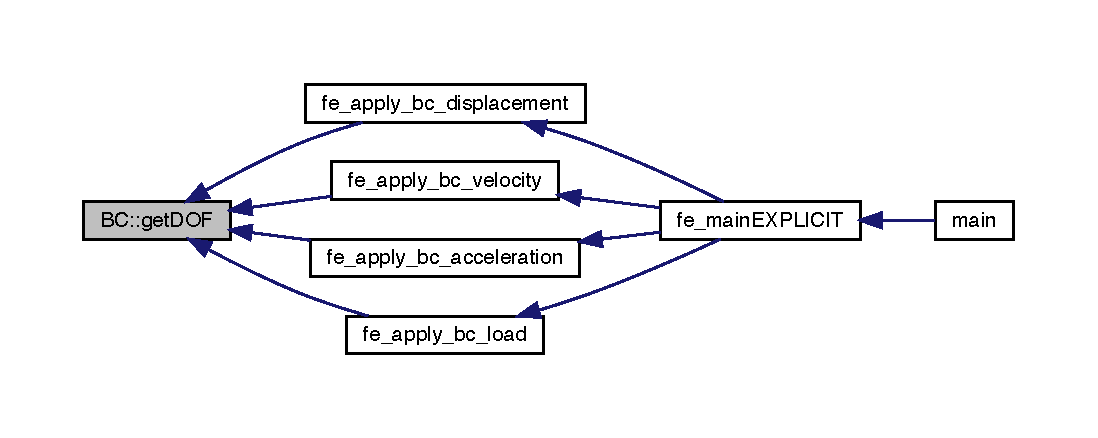
\includegraphics[width=350pt]{class_b_c_a0bc8eb90956a082ada5e4daa5e32c9fc_icgraph}
\end{center}
\end{figure}
\mbox{\Hypertarget{class_b_c_a6e42c3db5c67435bf2616768959866e9}\label{class_b_c_a6e42c3db5c67435bf2616768959866e9}} 
\index{BC@{BC}!get\+Num\+D\+OF@{get\+Num\+D\+OF}}
\index{get\+Num\+D\+OF@{get\+Num\+D\+OF}!BC@{BC}}
\subsubsection{\texorpdfstring{get\+Num\+D\+O\+F()}{getNumDOF()}}
{\footnotesize\ttfamily int B\+C\+::get\+Num\+D\+OF (\begin{DoxyParamCaption}{ }\end{DoxyParamCaption})}



Definition at line \hyperlink{_b_c_8cpp_source_l00022}{22} of file \hyperlink{_b_c_8cpp_source}{B\+C.\+cpp}.

Here is the caller graph for this function\+:\nopagebreak
\begin{figure}[H]
\begin{center}
\leavevmode
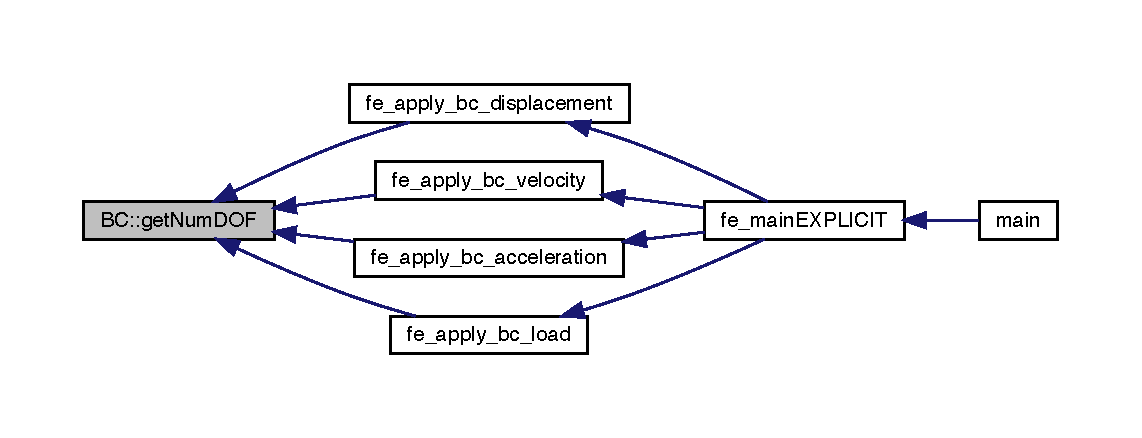
\includegraphics[width=350pt]{class_b_c_a6e42c3db5c67435bf2616768959866e9_icgraph}
\end{center}
\end{figure}
\mbox{\Hypertarget{class_b_c_a3590d0a29a9261d99f21ee75340e5722}\label{class_b_c_a3590d0a29a9261d99f21ee75340e5722}} 
\index{BC@{BC}!get\+Time\+Behavior@{get\+Time\+Behavior}}
\index{get\+Time\+Behavior@{get\+Time\+Behavior}!BC@{BC}}
\subsubsection{\texorpdfstring{get\+Time\+Behavior()}{getTimeBehavior()}}
{\footnotesize\ttfamily std\+::string B\+C\+::get\+Time\+Behavior (\begin{DoxyParamCaption}{ }\end{DoxyParamCaption})}



Definition at line \hyperlink{_b_c_8cpp_source_l00030}{30} of file \hyperlink{_b_c_8cpp_source}{B\+C.\+cpp}.

Here is the caller graph for this function\+:\nopagebreak
\begin{figure}[H]
\begin{center}
\leavevmode
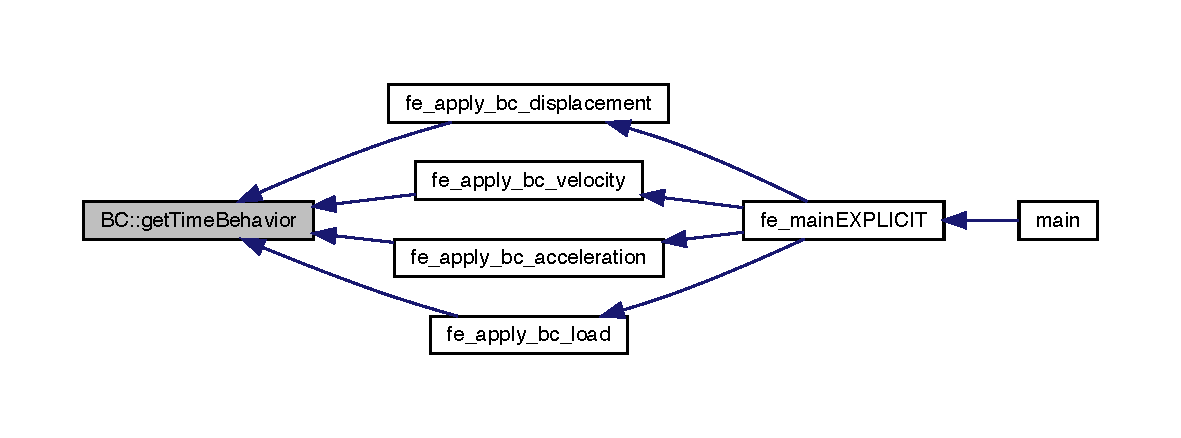
\includegraphics[width=350pt]{class_b_c_a3590d0a29a9261d99f21ee75340e5722_icgraph}
\end{center}
\end{figure}
\mbox{\Hypertarget{class_b_c_aa6afb3d4586f395578bef89c77e60449}\label{class_b_c_aa6afb3d4586f395578bef89c77e60449}} 
\index{BC@{BC}!get\+Type@{get\+Type}}
\index{get\+Type@{get\+Type}!BC@{BC}}
\subsubsection{\texorpdfstring{get\+Type()}{getType()}}
{\footnotesize\ttfamily std\+::string B\+C\+::get\+Type (\begin{DoxyParamCaption}{ }\end{DoxyParamCaption})}



Definition at line \hyperlink{_b_c_8cpp_source_l00014}{14} of file \hyperlink{_b_c_8cpp_source}{B\+C.\+cpp}.

Here is the caller graph for this function\+:\nopagebreak
\begin{figure}[H]
\begin{center}
\leavevmode
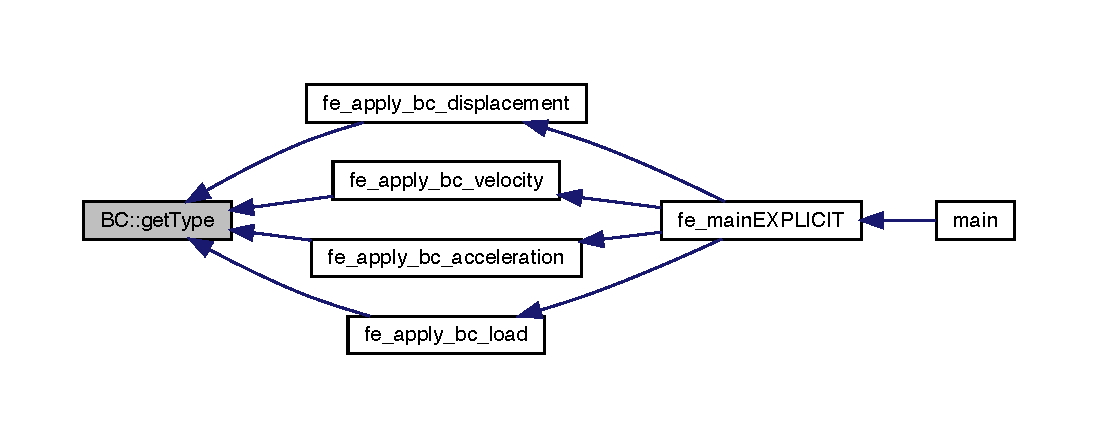
\includegraphics[width=350pt]{class_b_c_aa6afb3d4586f395578bef89c77e60449_icgraph}
\end{center}
\end{figure}
\mbox{\Hypertarget{class_b_c_a7f2fb6f9d3848e8f0617902b3fb804af}\label{class_b_c_a7f2fb6f9d3848e8f0617902b3fb804af}} 
\index{BC@{BC}!print\+B\+C\+Info@{print\+B\+C\+Info}}
\index{print\+B\+C\+Info@{print\+B\+C\+Info}!BC@{BC}}
\subsubsection{\texorpdfstring{print\+B\+C\+Info()}{printBCInfo()}}
{\footnotesize\ttfamily void B\+C\+::print\+B\+C\+Info (\begin{DoxyParamCaption}{ }\end{DoxyParamCaption})}



Definition at line \hyperlink{_b_c_8cpp_source_l00034}{34} of file \hyperlink{_b_c_8cpp_source}{B\+C.\+cpp}.

\mbox{\Hypertarget{class_b_c_a8ceaa781f98b4128fa50611ff9481e1a}\label{class_b_c_a8ceaa781f98b4128fa50611ff9481e1a}} 
\index{BC@{BC}!read\+BC@{read\+BC}}
\index{read\+BC@{read\+BC}!BC@{BC}}
\subsubsection{\texorpdfstring{read\+B\+C()}{readBC()}}
{\footnotesize\ttfamily void B\+C\+::read\+BC (\begin{DoxyParamCaption}\item[{std\+::string}]{type\+\_\+user,  }\item[{double}]{input\+\_\+amp\+\_\+user,  }\item[{int}]{num\+\_\+dof\+\_\+user,  }\item[{Vector\+Xi}]{dof\+\_\+user,  }\item[{std\+::string}]{time\+\_\+curve\+\_\+user }\end{DoxyParamCaption})}



Definition at line \hyperlink{_b_c_8cpp_source_l00006}{6} of file \hyperlink{_b_c_8cpp_source}{B\+C.\+cpp}.

Here is the caller graph for this function\+:\nopagebreak
\begin{figure}[H]
\begin{center}
\leavevmode
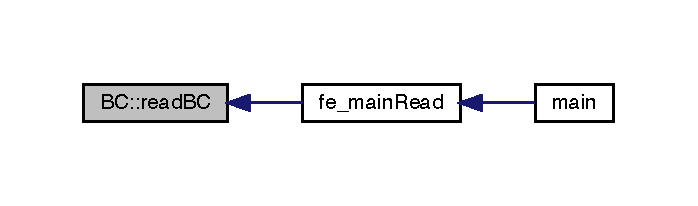
\includegraphics[width=335pt]{class_b_c_a8ceaa781f98b4128fa50611ff9481e1a_icgraph}
\end{center}
\end{figure}


\subsection{Member Data Documentation}
\mbox{\Hypertarget{class_b_c_a25d7def8fdf5e988602759608b1507ea}\label{class_b_c_a25d7def8fdf5e988602759608b1507ea}} 
\index{BC@{BC}!amplitude@{amplitude}}
\index{amplitude@{amplitude}!BC@{BC}}
\subsubsection{\texorpdfstring{amplitude}{amplitude}}
{\footnotesize\ttfamily double B\+C\+::amplitude\hspace{0.3cm}{\ttfamily [private]}}



Definition at line \hyperlink{_b_c_8h_source_l00019}{19} of file \hyperlink{_b_c_8h_source}{B\+C.\+h}.

\mbox{\Hypertarget{class_b_c_a4e53c8862da8b017b419b201911d9e00}\label{class_b_c_a4e53c8862da8b017b419b201911d9e00}} 
\index{BC@{BC}!dof@{dof}}
\index{dof@{dof}!BC@{BC}}
\subsubsection{\texorpdfstring{dof}{dof}}
{\footnotesize\ttfamily Vector\+Xi B\+C\+::dof\hspace{0.3cm}{\ttfamily [private]}}



Definition at line \hyperlink{_b_c_8h_source_l00021}{21} of file \hyperlink{_b_c_8h_source}{B\+C.\+h}.

\mbox{\Hypertarget{class_b_c_a71fe2e36793286c4e683a3d8485abaf2}\label{class_b_c_a71fe2e36793286c4e683a3d8485abaf2}} 
\index{BC@{BC}!num\+\_\+dof@{num\+\_\+dof}}
\index{num\+\_\+dof@{num\+\_\+dof}!BC@{BC}}
\subsubsection{\texorpdfstring{num\+\_\+dof}{num\_dof}}
{\footnotesize\ttfamily int B\+C\+::num\+\_\+dof\hspace{0.3cm}{\ttfamily [private]}}



Definition at line \hyperlink{_b_c_8h_source_l00020}{20} of file \hyperlink{_b_c_8h_source}{B\+C.\+h}.

\mbox{\Hypertarget{class_b_c_a84f989feaa5e81214f17b6dbdd1cf2ab}\label{class_b_c_a84f989feaa5e81214f17b6dbdd1cf2ab}} 
\index{BC@{BC}!time\+\_\+curve@{time\+\_\+curve}}
\index{time\+\_\+curve@{time\+\_\+curve}!BC@{BC}}
\subsubsection{\texorpdfstring{time\+\_\+curve}{time\_curve}}
{\footnotesize\ttfamily std\+::string B\+C\+::time\+\_\+curve\hspace{0.3cm}{\ttfamily [private]}}



Definition at line \hyperlink{_b_c_8h_source_l00022}{22} of file \hyperlink{_b_c_8h_source}{B\+C.\+h}.

\mbox{\Hypertarget{class_b_c_ab25297125dceec52f445a3a5efa77784}\label{class_b_c_ab25297125dceec52f445a3a5efa77784}} 
\index{BC@{BC}!type@{type}}
\index{type@{type}!BC@{BC}}
\subsubsection{\texorpdfstring{type}{type}}
{\footnotesize\ttfamily std\+::string B\+C\+::type\hspace{0.3cm}{\ttfamily [private]}}



Definition at line \hyperlink{_b_c_8h_source_l00018}{18} of file \hyperlink{_b_c_8h_source}{B\+C.\+h}.



The documentation for this class was generated from the following files\+:\begin{DoxyCompactItemize}
\item 
src/eema/include/\hyperlink{_b_c_8h}{B\+C.\+h}\item 
src/eema/src/\+Input-\/\+Output/\+Input/\hyperlink{_b_c_8cpp}{B\+C.\+cpp}\end{DoxyCompactItemize}

\hypertarget{class_materials}{}\section{Materials Class Reference}
\label{class_materials}\index{Materials@{Materials}}


{\ttfamily \#include $<$src/eema/include/\+Materials.\+h$>$}

\subsection*{Public Member Functions}
\begin{DoxyCompactItemize}
\item 
void \hyperlink{class_materials_a06e59a5742730b2292d39b7488523505}{read\+Mats} (int a, std\+::string b, Vector\+Xd c)
\item 
void \hyperlink{class_materials_acce0e8fc2993ca136273747fd75b8fc1}{print\+Mats} ()
\end{DoxyCompactItemize}
\subsection*{Private Attributes}
\begin{DoxyCompactItemize}
\item 
int \hyperlink{class_materials_a9687f294a4ae4b2603eed657ee7dbebf}{mat\+\_\+id}
\item 
std\+::string \hyperlink{class_materials_abe8d649257d71769de7a3aa20ff8977e}{mat\+\_\+model}
\item 
Vector\+Xd \hyperlink{class_materials_af663f6cf518ba3f857bac40a1e33eac0}{mat\+\_\+properties}
\item 
double \hyperlink{class_materials_ae1d76dc4fa0500285c6759f55038e4c6}{data}
\end{DoxyCompactItemize}
\subsection*{Friends}
\begin{DoxyCompactItemize}
\item 
double \hyperlink{class_materials_af7ffbad6dfcc99fc88b130c1a7b1720a}{fe\+\_\+get\+\_\+mats} (int matl\+\_\+code, int obj\+\_\+interest)
\item 
std\+::string \hyperlink{class_materials_a34d6fb85943d945b7e8600d2ef4220d0}{fe\+\_\+get\+\_\+model} (int matl\+\_\+code)
\end{DoxyCompactItemize}


\subsection{Detailed Description}


Definition at line \hyperlink{_materials_8h_source_l00023}{23} of file \hyperlink{_materials_8h_source}{Materials.\+h}.



\subsection{Member Function Documentation}
\mbox{\Hypertarget{class_materials_acce0e8fc2993ca136273747fd75b8fc1}\label{class_materials_acce0e8fc2993ca136273747fd75b8fc1}} 
\index{Materials@{Materials}!print\+Mats@{print\+Mats}}
\index{print\+Mats@{print\+Mats}!Materials@{Materials}}
\subsubsection{\texorpdfstring{print\+Mats()}{printMats()}}
{\footnotesize\ttfamily void Materials\+::print\+Mats (\begin{DoxyParamCaption}{ }\end{DoxyParamCaption})}



Definition at line \hyperlink{_materials_8cpp_source_l00015}{15} of file \hyperlink{_materials_8cpp_source}{Materials.\+cpp}.

\mbox{\Hypertarget{class_materials_a06e59a5742730b2292d39b7488523505}\label{class_materials_a06e59a5742730b2292d39b7488523505}} 
\index{Materials@{Materials}!read\+Mats@{read\+Mats}}
\index{read\+Mats@{read\+Mats}!Materials@{Materials}}
\subsubsection{\texorpdfstring{read\+Mats()}{readMats()}}
{\footnotesize\ttfamily void Materials\+::read\+Mats (\begin{DoxyParamCaption}\item[{int}]{a,  }\item[{std\+::string}]{b,  }\item[{Vector\+Xd}]{c }\end{DoxyParamCaption})}



Definition at line \hyperlink{_materials_8cpp_source_l00006}{6} of file \hyperlink{_materials_8cpp_source}{Materials.\+cpp}.

Here is the caller graph for this function\+:\nopagebreak
\begin{figure}[H]
\begin{center}
\leavevmode
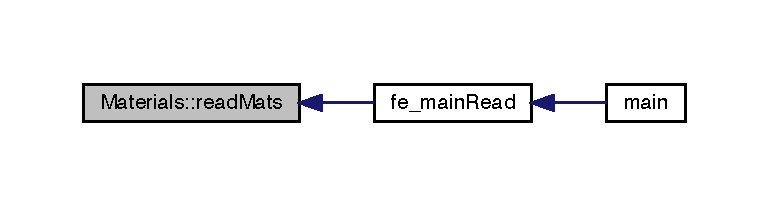
\includegraphics[width=350pt]{class_materials_a06e59a5742730b2292d39b7488523505_icgraph}
\end{center}
\end{figure}


\subsection{Friends And Related Function Documentation}
\mbox{\Hypertarget{class_materials_af7ffbad6dfcc99fc88b130c1a7b1720a}\label{class_materials_af7ffbad6dfcc99fc88b130c1a7b1720a}} 
\index{Materials@{Materials}!fe\+\_\+get\+\_\+mats@{fe\+\_\+get\+\_\+mats}}
\index{fe\+\_\+get\+\_\+mats@{fe\+\_\+get\+\_\+mats}!Materials@{Materials}}
\subsubsection{\texorpdfstring{fe\+\_\+get\+\_\+mats}{fe\_get\_mats}}
{\footnotesize\ttfamily double fe\+\_\+get\+\_\+mats (\begin{DoxyParamCaption}\item[{int}]{matl\+\_\+code,  }\item[{int}]{obj\+\_\+interest }\end{DoxyParamCaption})\hspace{0.3cm}{\ttfamily [friend]}}

Extracts the material parameter values based on the material id 

Definition at line \hyperlink{fe__get__mats_8cpp_source_l00005}{5} of file \hyperlink{fe__get__mats_8cpp_source}{fe\+\_\+get\+\_\+mats.\+cpp}.

\mbox{\Hypertarget{class_materials_a34d6fb85943d945b7e8600d2ef4220d0}\label{class_materials_a34d6fb85943d945b7e8600d2ef4220d0}} 
\index{Materials@{Materials}!fe\+\_\+get\+\_\+model@{fe\+\_\+get\+\_\+model}}
\index{fe\+\_\+get\+\_\+model@{fe\+\_\+get\+\_\+model}!Materials@{Materials}}
\subsubsection{\texorpdfstring{fe\+\_\+get\+\_\+model}{fe\_get\_model}}
{\footnotesize\ttfamily std\+::string fe\+\_\+get\+\_\+model (\begin{DoxyParamCaption}\item[{int}]{matl\+\_\+code }\end{DoxyParamCaption})\hspace{0.3cm}{\ttfamily [friend]}}

Extracts the material model name 

Definition at line \hyperlink{fe__get__model_8cpp_source_l00005}{5} of file \hyperlink{fe__get__model_8cpp_source}{fe\+\_\+get\+\_\+model.\+cpp}.



\subsection{Member Data Documentation}
\mbox{\Hypertarget{class_materials_ae1d76dc4fa0500285c6759f55038e4c6}\label{class_materials_ae1d76dc4fa0500285c6759f55038e4c6}} 
\index{Materials@{Materials}!data@{data}}
\index{data@{data}!Materials@{Materials}}
\subsubsection{\texorpdfstring{data}{data}}
{\footnotesize\ttfamily double Materials\+::data\hspace{0.3cm}{\ttfamily [private]}}



Definition at line \hyperlink{_materials_8h_source_l00029}{29} of file \hyperlink{_materials_8h_source}{Materials.\+h}.

\mbox{\Hypertarget{class_materials_a9687f294a4ae4b2603eed657ee7dbebf}\label{class_materials_a9687f294a4ae4b2603eed657ee7dbebf}} 
\index{Materials@{Materials}!mat\+\_\+id@{mat\+\_\+id}}
\index{mat\+\_\+id@{mat\+\_\+id}!Materials@{Materials}}
\subsubsection{\texorpdfstring{mat\+\_\+id}{mat\_id}}
{\footnotesize\ttfamily int Materials\+::mat\+\_\+id\hspace{0.3cm}{\ttfamily [private]}}



Definition at line \hyperlink{_materials_8h_source_l00025}{25} of file \hyperlink{_materials_8h_source}{Materials.\+h}.

\mbox{\Hypertarget{class_materials_abe8d649257d71769de7a3aa20ff8977e}\label{class_materials_abe8d649257d71769de7a3aa20ff8977e}} 
\index{Materials@{Materials}!mat\+\_\+model@{mat\+\_\+model}}
\index{mat\+\_\+model@{mat\+\_\+model}!Materials@{Materials}}
\subsubsection{\texorpdfstring{mat\+\_\+model}{mat\_model}}
{\footnotesize\ttfamily std\+::string Materials\+::mat\+\_\+model\hspace{0.3cm}{\ttfamily [private]}}



Definition at line \hyperlink{_materials_8h_source_l00026}{26} of file \hyperlink{_materials_8h_source}{Materials.\+h}.

\mbox{\Hypertarget{class_materials_af663f6cf518ba3f857bac40a1e33eac0}\label{class_materials_af663f6cf518ba3f857bac40a1e33eac0}} 
\index{Materials@{Materials}!mat\+\_\+properties@{mat\+\_\+properties}}
\index{mat\+\_\+properties@{mat\+\_\+properties}!Materials@{Materials}}
\subsubsection{\texorpdfstring{mat\+\_\+properties}{mat\_properties}}
{\footnotesize\ttfamily Vector\+Xd Materials\+::mat\+\_\+properties\hspace{0.3cm}{\ttfamily [private]}}



Definition at line \hyperlink{_materials_8h_source_l00027}{27} of file \hyperlink{_materials_8h_source}{Materials.\+h}.



The documentation for this class was generated from the following files\+:\begin{DoxyCompactItemize}
\item 
src/eema/include/\hyperlink{_materials_8h}{Materials.\+h}\item 
src/eema/src/\+Input-\/\+Output/\+Input/\hyperlink{_materials_8cpp}{Materials.\+cpp}\end{DoxyCompactItemize}

\hypertarget{class_mesh}{}\section{Mesh Class Reference}
\label{class_mesh}\index{Mesh@{Mesh}}


{\ttfamily \#include $<$src/eema/include/\+Mesh.\+h$>$}

\subsection*{Public Member Functions}
\begin{DoxyCompactItemize}
\item 
void \hyperlink{class_mesh_aba57df50d740f660cadf00aefe75e157}{read\+Mesh} (Matrix\+Xd n, Matrix\+Xi e)
\item 
void \hyperlink{class_mesh_a2193a797388525febbac794d17bea23e}{read\+Nodal\+Kinematics} (Vector\+Xd Usystem, Vector\+Xd Vsystem, Vector\+Xd Asystem)
\item 
void \hyperlink{class_mesh_a2c1456f1b3b5bda8d213624e3943dbb3}{read\+Stress\+Strain} (Matrix\+Xd stress\+\_\+tmp, Matrix\+Xd strain\+\_\+tmp)
\item 
Matrix\+Xd \hyperlink{class_mesh_a0b0f7458f07745240d9bda967cda12de}{get\+Nodes} ()
\item 
Matrix\+Xi \hyperlink{class_mesh_a4828631f942fd5a701870beea870f413}{get\+Elements} ()
\item 
Matrix\+Xd \hyperlink{class_mesh_a52ecce406bbef80cbf3610db3ea5ea40}{get\+New\+Nodes} ()
\item 
Matrix\+Xi \hyperlink{class_mesh_a6e425e9499e64ab52c4555aa3763651d}{get\+New\+Elements} ()
\item 
Vector\+Xd \hyperlink{class_mesh_a72d2a3863b85a2a2aed7deca8ce37832}{get\+Max\+Char\+Length} (std\+::string choice)
\begin{DoxyCompactList}\small\item\em Calculates the maximum charateristic length of the mesh. \end{DoxyCompactList}\item 
Vector\+Xd \hyperlink{class_mesh_a94ce58cb2598b1db2973ad357dae2710}{get\+Min\+Char\+Length} (std\+::string choice)
\begin{DoxyCompactList}\small\item\em Calculates the minimum charateristic length of the mesh. \end{DoxyCompactList}\item 
Vector\+Xd \hyperlink{class_mesh_a3fbc4b3c21f738efc6cdf3d02e31ad23}{get\+Nodal\+Disp} ()
\item 
Vector\+Xd \hyperlink{class_mesh_a052cd330cb8ccecf63e960a7afd0a6d9}{get\+Nodal\+Vel} ()
\item 
Vector\+Xd \hyperlink{class_mesh_ad41670edd4e6335071012837a58fb725}{get\+Nodal\+Acc} ()
\item 
Matrix\+Xd \hyperlink{class_mesh_a4ec62fd7219adcd406a167c1f6ee81e8}{get\+Cell\+Stress} ()
\item 
Matrix\+Xd \hyperlink{class_mesh_a1c54802401d00d14b390db2f0e615ebb}{get\+Cell\+Strain} ()
\item 
void \hyperlink{class_mesh_aa8a6f260e9589be4c0a2fcc146e696d5}{preprocess\+Mesh} ()
\item 
void \hyperlink{class_mesh_af03b49cbaf762652c9ff5ff7f4a6e668}{replace\+Nodes} (Matrix\+Xd \hyperlink{class_mesh_ae7202a4f96820433c69bc2ea4cc1b31d}{A}, std\+::string B)
\item 
void \hyperlink{class_mesh_a95ba7a96ec42ea4e0c191890f7faa2ab}{replace\+Elements} (Matrix\+Xi \hyperlink{class_mesh_ae7202a4f96820433c69bc2ea4cc1b31d}{A}, std\+::string B)
\item 
void \hyperlink{class_mesh_a894e41dd4280dfba75406eb8d0338a8e}{check\+Mesh} ()
\begin{DoxyCompactList}\small\item\em Check the mesh for zero charateristic lengths. \end{DoxyCompactList}\end{DoxyCompactItemize}
\subsection*{Private Attributes}
\begin{DoxyCompactItemize}
\item 
Matrix\+Xd \hyperlink{class_mesh_aa143447b8630a7a8bf2b045fddf372c3}{nodes}
\item 
Matrix\+Xi \hyperlink{class_mesh_a32aed9620eeb7eaf93a3f8c8f6e79bde}{elements}
\item 
Matrix\+Xd \hyperlink{class_mesh_aa9cae59f50d13339ed395ef567401cb8}{nodes\+\_\+new}
\item 
Matrix\+Xi \hyperlink{class_mesh_a8e099460dded463a5c13fb8d6066d312}{elements\+\_\+new}
\item 
Vector\+Xd \hyperlink{class_mesh_a950948f115bf07df771fa277042eedc1}{U}
\item 
Vector\+Xd \hyperlink{class_mesh_a69a99942ef6672d74a7ba569bdbd3c83}{V}
\item 
Vector\+Xd \hyperlink{class_mesh_ae7202a4f96820433c69bc2ea4cc1b31d}{A}
\item 
Matrix\+Xd \hyperlink{class_mesh_ae8f28f2627eeb9eccd9adcbdee1b2aa9}{stress}
\item 
Matrix\+Xd \hyperlink{class_mesh_a602850c13e7383308be4e65acd5b30fe}{strain}
\end{DoxyCompactItemize}


\subsection{Detailed Description}


Definition at line \hyperlink{_mesh_8h_source_l00023}{23} of file \hyperlink{_mesh_8h_source}{Mesh.\+h}.



\subsection{Member Function Documentation}
\mbox{\Hypertarget{class_mesh_a894e41dd4280dfba75406eb8d0338a8e}\label{class_mesh_a894e41dd4280dfba75406eb8d0338a8e}} 
\index{Mesh@{Mesh}!check\+Mesh@{check\+Mesh}}
\index{check\+Mesh@{check\+Mesh}!Mesh@{Mesh}}
\subsubsection{\texorpdfstring{check\+Mesh()}{checkMesh()}}
{\footnotesize\ttfamily void Mesh\+::check\+Mesh (\begin{DoxyParamCaption}{ }\end{DoxyParamCaption})}



Check the mesh for zero charateristic lengths. 



Definition at line \hyperlink{_mesh_8cpp_source_l00208}{208} of file \hyperlink{_mesh_8cpp_source}{Mesh.\+cpp}.

Here is the caller graph for this function\+:\nopagebreak
\begin{figure}[H]
\begin{center}
\leavevmode
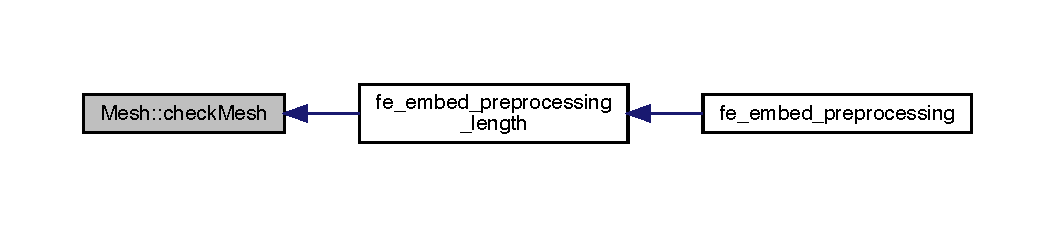
\includegraphics[width=350pt]{class_mesh_a894e41dd4280dfba75406eb8d0338a8e_icgraph}
\end{center}
\end{figure}
\mbox{\Hypertarget{class_mesh_a1c54802401d00d14b390db2f0e615ebb}\label{class_mesh_a1c54802401d00d14b390db2f0e615ebb}} 
\index{Mesh@{Mesh}!get\+Cell\+Strain@{get\+Cell\+Strain}}
\index{get\+Cell\+Strain@{get\+Cell\+Strain}!Mesh@{Mesh}}
\subsubsection{\texorpdfstring{get\+Cell\+Strain()}{getCellStrain()}}
{\footnotesize\ttfamily Matrix\+Xd Mesh\+::get\+Cell\+Strain (\begin{DoxyParamCaption}{ }\end{DoxyParamCaption})}

Ouputs element-\/wise strain of the entire mesh 

Definition at line \hyperlink{_mesh_8cpp_source_l00054}{54} of file \hyperlink{_mesh_8cpp_source}{Mesh.\+cpp}.

Here is the caller graph for this function\+:\nopagebreak
\begin{figure}[H]
\begin{center}
\leavevmode
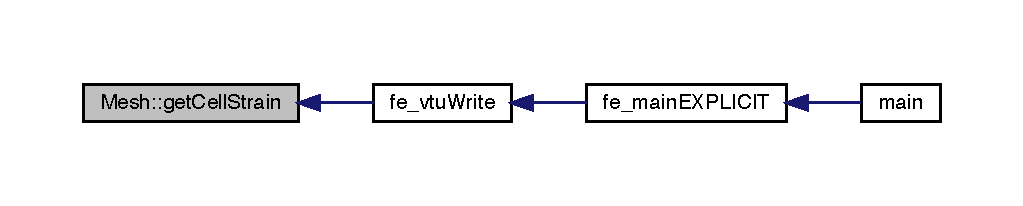
\includegraphics[width=350pt]{class_mesh_a1c54802401d00d14b390db2f0e615ebb_icgraph}
\end{center}
\end{figure}
\mbox{\Hypertarget{class_mesh_a4ec62fd7219adcd406a167c1f6ee81e8}\label{class_mesh_a4ec62fd7219adcd406a167c1f6ee81e8}} 
\index{Mesh@{Mesh}!get\+Cell\+Stress@{get\+Cell\+Stress}}
\index{get\+Cell\+Stress@{get\+Cell\+Stress}!Mesh@{Mesh}}
\subsubsection{\texorpdfstring{get\+Cell\+Stress()}{getCellStress()}}
{\footnotesize\ttfamily Matrix\+Xd Mesh\+::get\+Cell\+Stress (\begin{DoxyParamCaption}{ }\end{DoxyParamCaption})}

Outputs element-\/wise stress of the mesh 

Definition at line \hyperlink{_mesh_8cpp_source_l00050}{50} of file \hyperlink{_mesh_8cpp_source}{Mesh.\+cpp}.

Here is the caller graph for this function\+:\nopagebreak
\begin{figure}[H]
\begin{center}
\leavevmode
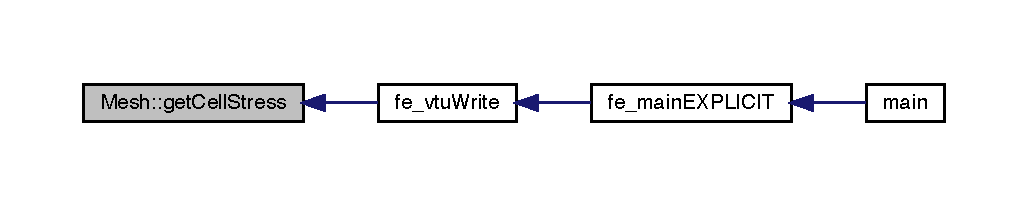
\includegraphics[width=350pt]{class_mesh_a4ec62fd7219adcd406a167c1f6ee81e8_icgraph}
\end{center}
\end{figure}
\mbox{\Hypertarget{class_mesh_a4828631f942fd5a701870beea870f413}\label{class_mesh_a4828631f942fd5a701870beea870f413}} 
\index{Mesh@{Mesh}!get\+Elements@{get\+Elements}}
\index{get\+Elements@{get\+Elements}!Mesh@{Mesh}}
\subsubsection{\texorpdfstring{get\+Elements()}{getElements()}}
{\footnotesize\ttfamily Matrix\+Xi Mesh\+::get\+Elements (\begin{DoxyParamCaption}\item[{void}]{ }\end{DoxyParamCaption})}



Definition at line \hyperlink{_mesh_8cpp_source_l00015}{15} of file \hyperlink{_mesh_8cpp_source}{Mesh.\+cpp}.

\mbox{\Hypertarget{class_mesh_a72d2a3863b85a2a2aed7deca8ce37832}\label{class_mesh_a72d2a3863b85a2a2aed7deca8ce37832}} 
\index{Mesh@{Mesh}!get\+Max\+Char\+Length@{get\+Max\+Char\+Length}}
\index{get\+Max\+Char\+Length@{get\+Max\+Char\+Length}!Mesh@{Mesh}}
\subsubsection{\texorpdfstring{get\+Max\+Char\+Length()}{getMaxCharLength()}}
{\footnotesize\ttfamily Vector\+Xd Mesh\+::get\+Max\+Char\+Length (\begin{DoxyParamCaption}\item[{std\+::string}]{choice }\end{DoxyParamCaption})}



Calculates the maximum charateristic length of the mesh. 



Definition at line \hyperlink{_mesh_8cpp_source_l00153}{153} of file \hyperlink{_mesh_8cpp_source}{Mesh.\+cpp}.

Here is the call graph for this function\+:\nopagebreak
\begin{figure}[H]
\begin{center}
\leavevmode
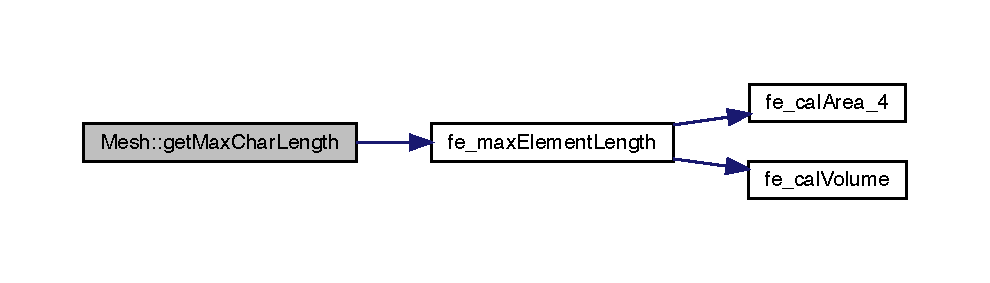
\includegraphics[width=350pt]{class_mesh_a72d2a3863b85a2a2aed7deca8ce37832_cgraph}
\end{center}
\end{figure}
Here is the caller graph for this function\+:\nopagebreak
\begin{figure}[H]
\begin{center}
\leavevmode
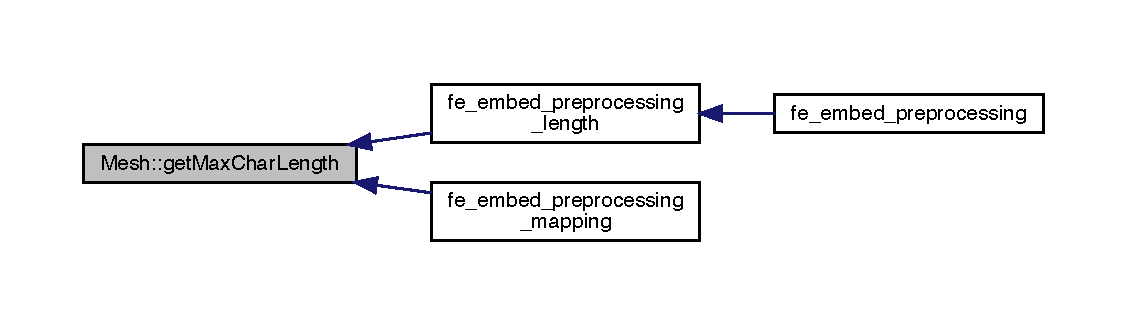
\includegraphics[width=350pt]{class_mesh_a72d2a3863b85a2a2aed7deca8ce37832_icgraph}
\end{center}
\end{figure}
\mbox{\Hypertarget{class_mesh_a94ce58cb2598b1db2973ad357dae2710}\label{class_mesh_a94ce58cb2598b1db2973ad357dae2710}} 
\index{Mesh@{Mesh}!get\+Min\+Char\+Length@{get\+Min\+Char\+Length}}
\index{get\+Min\+Char\+Length@{get\+Min\+Char\+Length}!Mesh@{Mesh}}
\subsubsection{\texorpdfstring{get\+Min\+Char\+Length()}{getMinCharLength()}}
{\footnotesize\ttfamily Vector\+Xd Mesh\+::get\+Min\+Char\+Length (\begin{DoxyParamCaption}\item[{std\+::string}]{choice }\end{DoxyParamCaption})}



Calculates the minimum charateristic length of the mesh. 



Definition at line \hyperlink{_mesh_8cpp_source_l00097}{97} of file \hyperlink{_mesh_8cpp_source}{Mesh.\+cpp}.

Here is the call graph for this function\+:\nopagebreak
\begin{figure}[H]
\begin{center}
\leavevmode
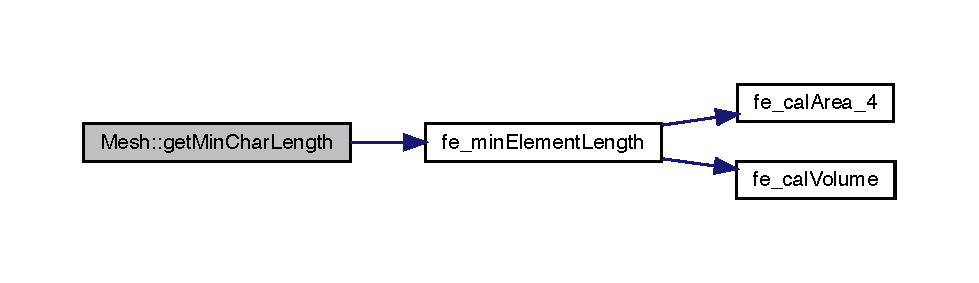
\includegraphics[width=350pt]{class_mesh_a94ce58cb2598b1db2973ad357dae2710_cgraph}
\end{center}
\end{figure}
Here is the caller graph for this function\+:\nopagebreak
\begin{figure}[H]
\begin{center}
\leavevmode
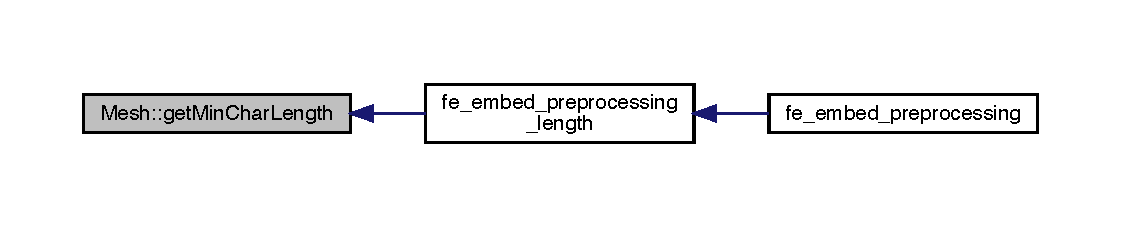
\includegraphics[width=350pt]{class_mesh_a94ce58cb2598b1db2973ad357dae2710_icgraph}
\end{center}
\end{figure}
\mbox{\Hypertarget{class_mesh_a6e425e9499e64ab52c4555aa3763651d}\label{class_mesh_a6e425e9499e64ab52c4555aa3763651d}} 
\index{Mesh@{Mesh}!get\+New\+Elements@{get\+New\+Elements}}
\index{get\+New\+Elements@{get\+New\+Elements}!Mesh@{Mesh}}
\subsubsection{\texorpdfstring{get\+New\+Elements()}{getNewElements()}}
{\footnotesize\ttfamily Matrix\+Xi Mesh\+::get\+New\+Elements (\begin{DoxyParamCaption}\item[{void}]{ }\end{DoxyParamCaption})}



Definition at line \hyperlink{_mesh_8cpp_source_l00023}{23} of file \hyperlink{_mesh_8cpp_source}{Mesh.\+cpp}.

Here is the caller graph for this function\+:\nopagebreak
\begin{figure}[H]
\begin{center}
\leavevmode
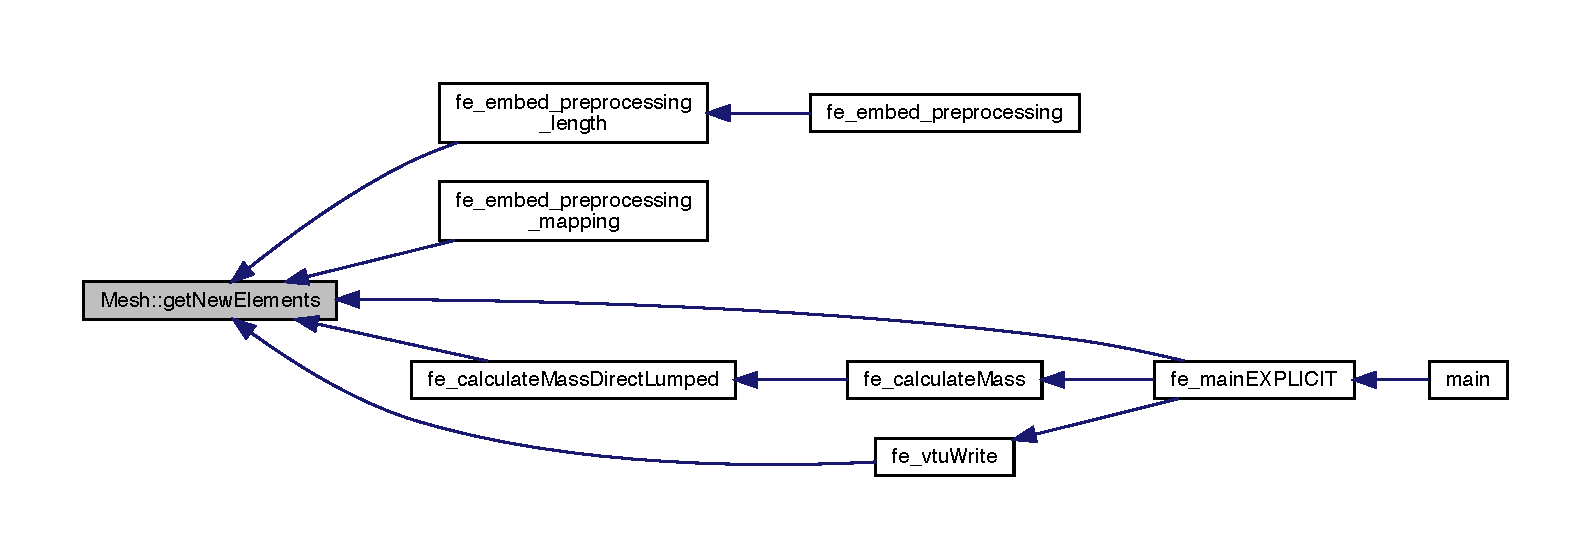
\includegraphics[width=350pt]{class_mesh_a6e425e9499e64ab52c4555aa3763651d_icgraph}
\end{center}
\end{figure}
\mbox{\Hypertarget{class_mesh_a52ecce406bbef80cbf3610db3ea5ea40}\label{class_mesh_a52ecce406bbef80cbf3610db3ea5ea40}} 
\index{Mesh@{Mesh}!get\+New\+Nodes@{get\+New\+Nodes}}
\index{get\+New\+Nodes@{get\+New\+Nodes}!Mesh@{Mesh}}
\subsubsection{\texorpdfstring{get\+New\+Nodes()}{getNewNodes()}}
{\footnotesize\ttfamily Matrix\+Xd Mesh\+::get\+New\+Nodes (\begin{DoxyParamCaption}\item[{void}]{ }\end{DoxyParamCaption})}



Definition at line \hyperlink{_mesh_8cpp_source_l00019}{19} of file \hyperlink{_mesh_8cpp_source}{Mesh.\+cpp}.

Here is the caller graph for this function\+:\nopagebreak
\begin{figure}[H]
\begin{center}
\leavevmode
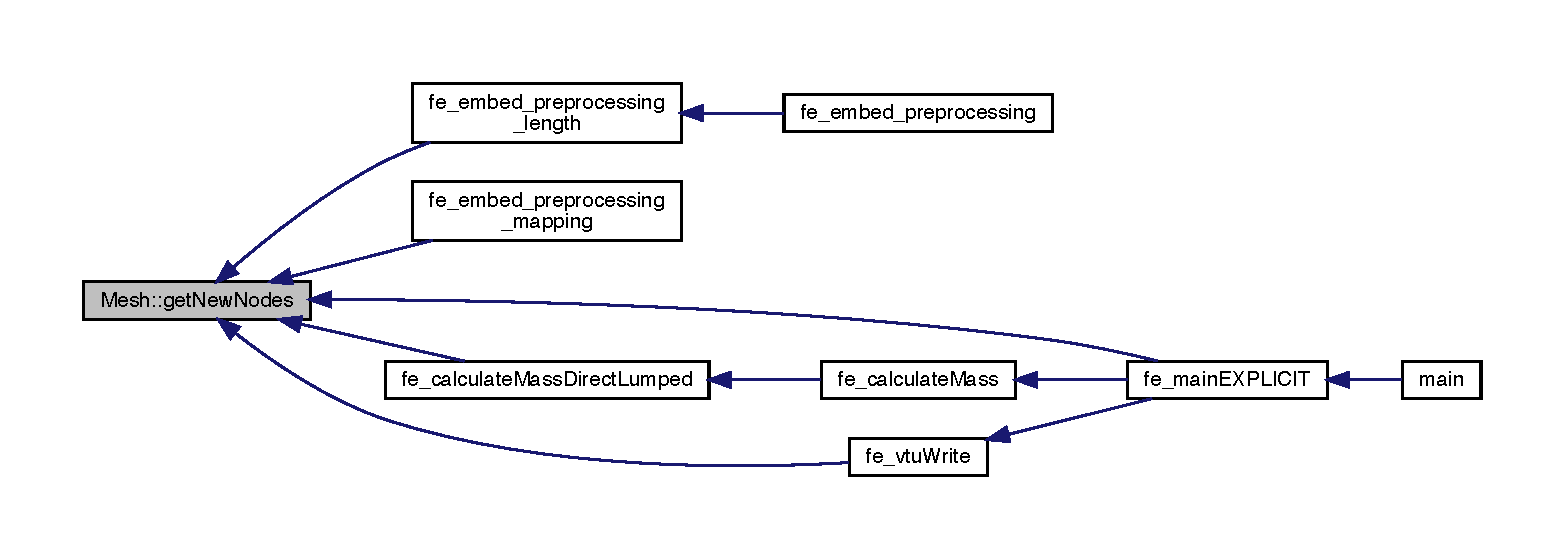
\includegraphics[width=350pt]{class_mesh_a52ecce406bbef80cbf3610db3ea5ea40_icgraph}
\end{center}
\end{figure}
\mbox{\Hypertarget{class_mesh_ad41670edd4e6335071012837a58fb725}\label{class_mesh_ad41670edd4e6335071012837a58fb725}} 
\index{Mesh@{Mesh}!get\+Nodal\+Acc@{get\+Nodal\+Acc}}
\index{get\+Nodal\+Acc@{get\+Nodal\+Acc}!Mesh@{Mesh}}
\subsubsection{\texorpdfstring{get\+Nodal\+Acc()}{getNodalAcc()}}
{\footnotesize\ttfamily Vector\+Xd Mesh\+::get\+Nodal\+Acc (\begin{DoxyParamCaption}\item[{void}]{ }\end{DoxyParamCaption})}

Outputs nodal acceleration vector 

Definition at line \hyperlink{_mesh_8cpp_source_l00041}{41} of file \hyperlink{_mesh_8cpp_source}{Mesh.\+cpp}.

Here is the caller graph for this function\+:\nopagebreak
\begin{figure}[H]
\begin{center}
\leavevmode
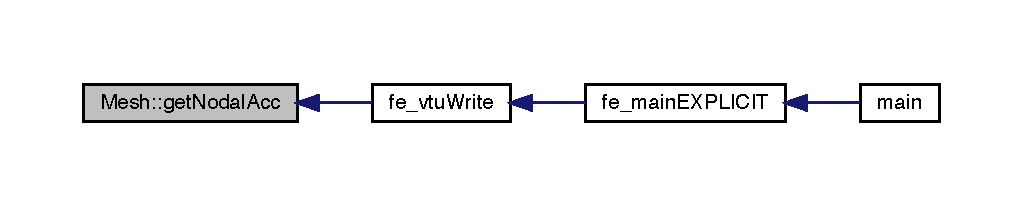
\includegraphics[width=350pt]{class_mesh_ad41670edd4e6335071012837a58fb725_icgraph}
\end{center}
\end{figure}
\mbox{\Hypertarget{class_mesh_a3fbc4b3c21f738efc6cdf3d02e31ad23}\label{class_mesh_a3fbc4b3c21f738efc6cdf3d02e31ad23}} 
\index{Mesh@{Mesh}!get\+Nodal\+Disp@{get\+Nodal\+Disp}}
\index{get\+Nodal\+Disp@{get\+Nodal\+Disp}!Mesh@{Mesh}}
\subsubsection{\texorpdfstring{get\+Nodal\+Disp()}{getNodalDisp()}}
{\footnotesize\ttfamily Vector\+Xd Mesh\+::get\+Nodal\+Disp (\begin{DoxyParamCaption}\item[{void}]{ }\end{DoxyParamCaption})}

Outputs nodal displacement vector 

Definition at line \hyperlink{_mesh_8cpp_source_l00033}{33} of file \hyperlink{_mesh_8cpp_source}{Mesh.\+cpp}.

Here is the caller graph for this function\+:\nopagebreak
\begin{figure}[H]
\begin{center}
\leavevmode
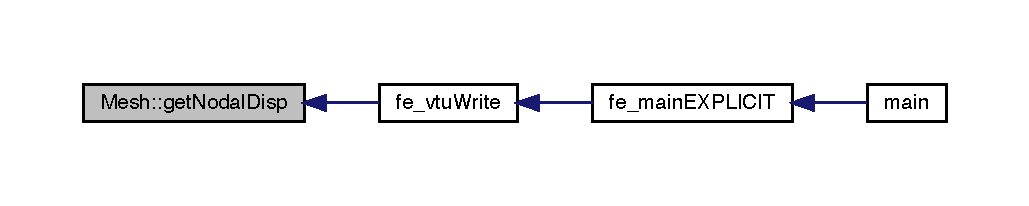
\includegraphics[width=350pt]{class_mesh_a3fbc4b3c21f738efc6cdf3d02e31ad23_icgraph}
\end{center}
\end{figure}
\mbox{\Hypertarget{class_mesh_a052cd330cb8ccecf63e960a7afd0a6d9}\label{class_mesh_a052cd330cb8ccecf63e960a7afd0a6d9}} 
\index{Mesh@{Mesh}!get\+Nodal\+Vel@{get\+Nodal\+Vel}}
\index{get\+Nodal\+Vel@{get\+Nodal\+Vel}!Mesh@{Mesh}}
\subsubsection{\texorpdfstring{get\+Nodal\+Vel()}{getNodalVel()}}
{\footnotesize\ttfamily Vector\+Xd Mesh\+::get\+Nodal\+Vel (\begin{DoxyParamCaption}\item[{void}]{ }\end{DoxyParamCaption})}

Outputs nodal velocity vector 

Definition at line \hyperlink{_mesh_8cpp_source_l00037}{37} of file \hyperlink{_mesh_8cpp_source}{Mesh.\+cpp}.

Here is the caller graph for this function\+:\nopagebreak
\begin{figure}[H]
\begin{center}
\leavevmode
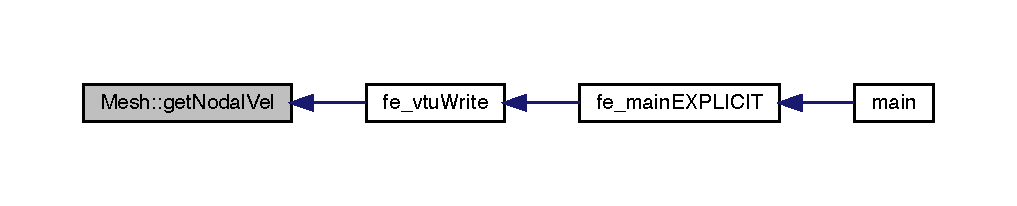
\includegraphics[width=350pt]{class_mesh_a052cd330cb8ccecf63e960a7afd0a6d9_icgraph}
\end{center}
\end{figure}
\mbox{\Hypertarget{class_mesh_a0b0f7458f07745240d9bda967cda12de}\label{class_mesh_a0b0f7458f07745240d9bda967cda12de}} 
\index{Mesh@{Mesh}!get\+Nodes@{get\+Nodes}}
\index{get\+Nodes@{get\+Nodes}!Mesh@{Mesh}}
\subsubsection{\texorpdfstring{get\+Nodes()}{getNodes()}}
{\footnotesize\ttfamily Matrix\+Xd Mesh\+::get\+Nodes (\begin{DoxyParamCaption}\item[{void}]{ }\end{DoxyParamCaption})}



Definition at line \hyperlink{_mesh_8cpp_source_l00011}{11} of file \hyperlink{_mesh_8cpp_source}{Mesh.\+cpp}.

\mbox{\Hypertarget{class_mesh_aa8a6f260e9589be4c0a2fcc146e696d5}\label{class_mesh_aa8a6f260e9589be4c0a2fcc146e696d5}} 
\index{Mesh@{Mesh}!preprocess\+Mesh@{preprocess\+Mesh}}
\index{preprocess\+Mesh@{preprocess\+Mesh}!Mesh@{Mesh}}
\subsubsection{\texorpdfstring{preprocess\+Mesh()}{preprocessMesh()}}
{\footnotesize\ttfamily void Mesh\+::preprocess\+Mesh (\begin{DoxyParamCaption}\item[{void}]{ }\end{DoxyParamCaption})}

Nodes Preprocessing -\/ Putting the numbering in order

Elements Preprocessing -\/ Correcting the element definitions 

Definition at line \hyperlink{_mesh_8cpp_source_l00058}{58} of file \hyperlink{_mesh_8cpp_source}{Mesh.\+cpp}.

Here is the caller graph for this function\+:\nopagebreak
\begin{figure}[H]
\begin{center}
\leavevmode
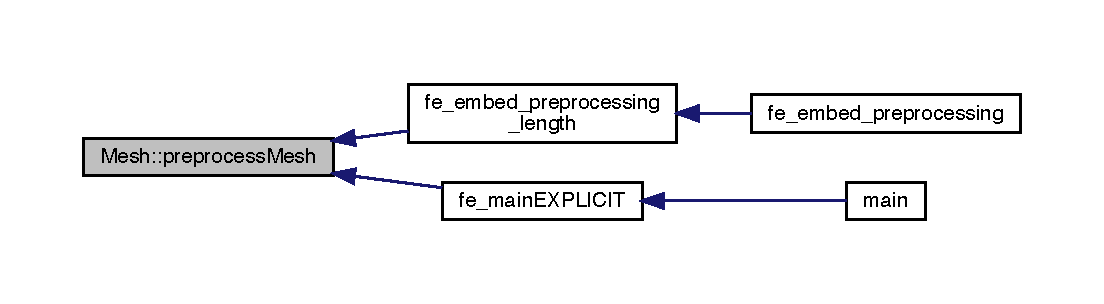
\includegraphics[width=350pt]{class_mesh_aa8a6f260e9589be4c0a2fcc146e696d5_icgraph}
\end{center}
\end{figure}
\mbox{\Hypertarget{class_mesh_aba57df50d740f660cadf00aefe75e157}\label{class_mesh_aba57df50d740f660cadf00aefe75e157}} 
\index{Mesh@{Mesh}!read\+Mesh@{read\+Mesh}}
\index{read\+Mesh@{read\+Mesh}!Mesh@{Mesh}}
\subsubsection{\texorpdfstring{read\+Mesh()}{readMesh()}}
{\footnotesize\ttfamily void Mesh\+::read\+Mesh (\begin{DoxyParamCaption}\item[{Matrix\+Xd}]{n,  }\item[{Matrix\+Xi}]{e }\end{DoxyParamCaption})}



Definition at line \hyperlink{_mesh_8cpp_source_l00006}{6} of file \hyperlink{_mesh_8cpp_source}{Mesh.\+cpp}.

Here is the caller graph for this function\+:\nopagebreak
\begin{figure}[H]
\begin{center}
\leavevmode
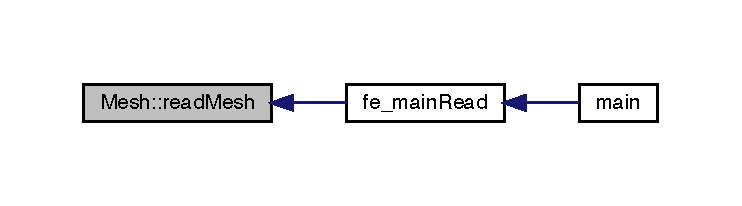
\includegraphics[width=350pt]{class_mesh_aba57df50d740f660cadf00aefe75e157_icgraph}
\end{center}
\end{figure}
\mbox{\Hypertarget{class_mesh_a2193a797388525febbac794d17bea23e}\label{class_mesh_a2193a797388525febbac794d17bea23e}} 
\index{Mesh@{Mesh}!read\+Nodal\+Kinematics@{read\+Nodal\+Kinematics}}
\index{read\+Nodal\+Kinematics@{read\+Nodal\+Kinematics}!Mesh@{Mesh}}
\subsubsection{\texorpdfstring{read\+Nodal\+Kinematics()}{readNodalKinematics()}}
{\footnotesize\ttfamily void Mesh\+::read\+Nodal\+Kinematics (\begin{DoxyParamCaption}\item[{Vector\+Xd}]{Usystem,  }\item[{Vector\+Xd}]{Vsystem,  }\item[{Vector\+Xd}]{Asystem }\end{DoxyParamCaption})}



Definition at line \hyperlink{_mesh_8cpp_source_l00027}{27} of file \hyperlink{_mesh_8cpp_source}{Mesh.\+cpp}.

Here is the caller graph for this function\+:\nopagebreak
\begin{figure}[H]
\begin{center}
\leavevmode
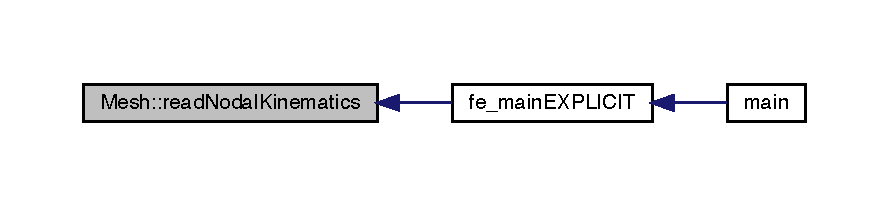
\includegraphics[width=350pt]{class_mesh_a2193a797388525febbac794d17bea23e_icgraph}
\end{center}
\end{figure}
\mbox{\Hypertarget{class_mesh_a2c1456f1b3b5bda8d213624e3943dbb3}\label{class_mesh_a2c1456f1b3b5bda8d213624e3943dbb3}} 
\index{Mesh@{Mesh}!read\+Stress\+Strain@{read\+Stress\+Strain}}
\index{read\+Stress\+Strain@{read\+Stress\+Strain}!Mesh@{Mesh}}
\subsubsection{\texorpdfstring{read\+Stress\+Strain()}{readStressStrain()}}
{\footnotesize\ttfamily void Mesh\+::read\+Stress\+Strain (\begin{DoxyParamCaption}\item[{Matrix\+Xd}]{stress\+\_\+tmp,  }\item[{Matrix\+Xd}]{strain\+\_\+tmp }\end{DoxyParamCaption})}



Definition at line \hyperlink{_mesh_8cpp_source_l00045}{45} of file \hyperlink{_mesh_8cpp_source}{Mesh.\+cpp}.

Here is the caller graph for this function\+:\nopagebreak
\begin{figure}[H]
\begin{center}
\leavevmode
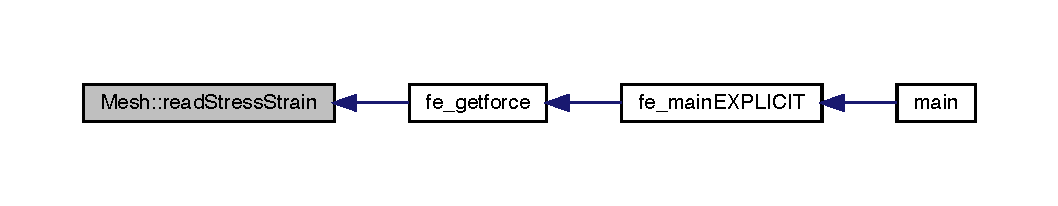
\includegraphics[width=350pt]{class_mesh_a2c1456f1b3b5bda8d213624e3943dbb3_icgraph}
\end{center}
\end{figure}
\mbox{\Hypertarget{class_mesh_a95ba7a96ec42ea4e0c191890f7faa2ab}\label{class_mesh_a95ba7a96ec42ea4e0c191890f7faa2ab}} 
\index{Mesh@{Mesh}!replace\+Elements@{replace\+Elements}}
\index{replace\+Elements@{replace\+Elements}!Mesh@{Mesh}}
\subsubsection{\texorpdfstring{replace\+Elements()}{replaceElements()}}
{\footnotesize\ttfamily void Mesh\+::replace\+Elements (\begin{DoxyParamCaption}\item[{Matrix\+Xi}]{A,  }\item[{std\+::string}]{B }\end{DoxyParamCaption})}



Definition at line \hyperlink{_mesh_8cpp_source_l00086}{86} of file \hyperlink{_mesh_8cpp_source}{Mesh.\+cpp}.

Here is the caller graph for this function\+:\nopagebreak
\begin{figure}[H]
\begin{center}
\leavevmode
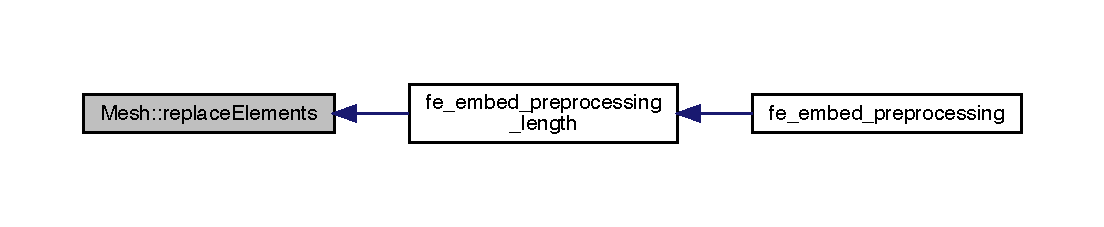
\includegraphics[width=350pt]{class_mesh_a95ba7a96ec42ea4e0c191890f7faa2ab_icgraph}
\end{center}
\end{figure}
\mbox{\Hypertarget{class_mesh_af03b49cbaf762652c9ff5ff7f4a6e668}\label{class_mesh_af03b49cbaf762652c9ff5ff7f4a6e668}} 
\index{Mesh@{Mesh}!replace\+Nodes@{replace\+Nodes}}
\index{replace\+Nodes@{replace\+Nodes}!Mesh@{Mesh}}
\subsubsection{\texorpdfstring{replace\+Nodes()}{replaceNodes()}}
{\footnotesize\ttfamily void Mesh\+::replace\+Nodes (\begin{DoxyParamCaption}\item[{Matrix\+Xd}]{A,  }\item[{std\+::string}]{B }\end{DoxyParamCaption})}



Definition at line \hyperlink{_mesh_8cpp_source_l00076}{76} of file \hyperlink{_mesh_8cpp_source}{Mesh.\+cpp}.

Here is the caller graph for this function\+:\nopagebreak
\begin{figure}[H]
\begin{center}
\leavevmode
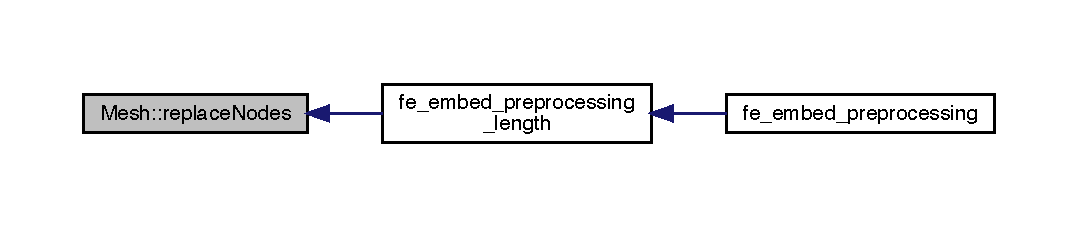
\includegraphics[width=350pt]{class_mesh_af03b49cbaf762652c9ff5ff7f4a6e668_icgraph}
\end{center}
\end{figure}


\subsection{Member Data Documentation}
\mbox{\Hypertarget{class_mesh_ae7202a4f96820433c69bc2ea4cc1b31d}\label{class_mesh_ae7202a4f96820433c69bc2ea4cc1b31d}} 
\index{Mesh@{Mesh}!A@{A}}
\index{A@{A}!Mesh@{Mesh}}
\subsubsection{\texorpdfstring{A}{A}}
{\footnotesize\ttfamily Vector\+Xd Mesh\+::A\hspace{0.3cm}{\ttfamily [private]}}

\hyperlink{class_mesh}{Mesh} -\/ Nodal Acceleration Vector. This Vector stores the nodal displacement at one time point only. 

Definition at line \hyperlink{_mesh_8h_source_l00040}{40} of file \hyperlink{_mesh_8h_source}{Mesh.\+h}.

\mbox{\Hypertarget{class_mesh_a32aed9620eeb7eaf93a3f8c8f6e79bde}\label{class_mesh_a32aed9620eeb7eaf93a3f8c8f6e79bde}} 
\index{Mesh@{Mesh}!elements@{elements}}
\index{elements@{elements}!Mesh@{Mesh}}
\subsubsection{\texorpdfstring{elements}{elements}}
{\footnotesize\ttfamily Matrix\+Xi Mesh\+::elements\hspace{0.3cm}{\ttfamily [private]}}

This contains the element data read from the mesh 

Definition at line \hyperlink{_mesh_8h_source_l00027}{27} of file \hyperlink{_mesh_8h_source}{Mesh.\+h}.

\mbox{\Hypertarget{class_mesh_a8e099460dded463a5c13fb8d6066d312}\label{class_mesh_a8e099460dded463a5c13fb8d6066d312}} 
\index{Mesh@{Mesh}!elements\+\_\+new@{elements\+\_\+new}}
\index{elements\+\_\+new@{elements\+\_\+new}!Mesh@{Mesh}}
\subsubsection{\texorpdfstring{elements\+\_\+new}{elements\_new}}
{\footnotesize\ttfamily Matrix\+Xi Mesh\+::elements\+\_\+new\hspace{0.3cm}{\ttfamily [private]}}

This contains the element data after preprocessing or any other operation 

Definition at line \hyperlink{_mesh_8h_source_l00031}{31} of file \hyperlink{_mesh_8h_source}{Mesh.\+h}.

\mbox{\Hypertarget{class_mesh_aa143447b8630a7a8bf2b045fddf372c3}\label{class_mesh_aa143447b8630a7a8bf2b045fddf372c3}} 
\index{Mesh@{Mesh}!nodes@{nodes}}
\index{nodes@{nodes}!Mesh@{Mesh}}
\subsubsection{\texorpdfstring{nodes}{nodes}}
{\footnotesize\ttfamily Matrix\+Xd Mesh\+::nodes\hspace{0.3cm}{\ttfamily [private]}}

This contains the nodal data read from the mesh 

Definition at line \hyperlink{_mesh_8h_source_l00025}{25} of file \hyperlink{_mesh_8h_source}{Mesh.\+h}.

\mbox{\Hypertarget{class_mesh_aa9cae59f50d13339ed395ef567401cb8}\label{class_mesh_aa9cae59f50d13339ed395ef567401cb8}} 
\index{Mesh@{Mesh}!nodes\+\_\+new@{nodes\+\_\+new}}
\index{nodes\+\_\+new@{nodes\+\_\+new}!Mesh@{Mesh}}
\subsubsection{\texorpdfstring{nodes\+\_\+new}{nodes\_new}}
{\footnotesize\ttfamily Matrix\+Xd Mesh\+::nodes\+\_\+new\hspace{0.3cm}{\ttfamily [private]}}

This contains the nodal data after preprocessing or any other operation 

Definition at line \hyperlink{_mesh_8h_source_l00029}{29} of file \hyperlink{_mesh_8h_source}{Mesh.\+h}.

\mbox{\Hypertarget{class_mesh_a602850c13e7383308be4e65acd5b30fe}\label{class_mesh_a602850c13e7383308be4e65acd5b30fe}} 
\index{Mesh@{Mesh}!strain@{strain}}
\index{strain@{strain}!Mesh@{Mesh}}
\subsubsection{\texorpdfstring{strain}{strain}}
{\footnotesize\ttfamily Matrix\+Xd Mesh\+::strain\hspace{0.3cm}{\ttfamily [private]}}

\hyperlink{class_mesh}{Mesh} -\/ Element-\/wise strain vector 

Definition at line \hyperlink{_mesh_8h_source_l00046}{46} of file \hyperlink{_mesh_8h_source}{Mesh.\+h}.

\mbox{\Hypertarget{class_mesh_ae8f28f2627eeb9eccd9adcbdee1b2aa9}\label{class_mesh_ae8f28f2627eeb9eccd9adcbdee1b2aa9}} 
\index{Mesh@{Mesh}!stress@{stress}}
\index{stress@{stress}!Mesh@{Mesh}}
\subsubsection{\texorpdfstring{stress}{stress}}
{\footnotesize\ttfamily Matrix\+Xd Mesh\+::stress\hspace{0.3cm}{\ttfamily [private]}}

\hyperlink{class_mesh}{Mesh} -\/ Element-\/wise stress vector 

Definition at line \hyperlink{_mesh_8h_source_l00043}{43} of file \hyperlink{_mesh_8h_source}{Mesh.\+h}.

\mbox{\Hypertarget{class_mesh_a950948f115bf07df771fa277042eedc1}\label{class_mesh_a950948f115bf07df771fa277042eedc1}} 
\index{Mesh@{Mesh}!U@{U}}
\index{U@{U}!Mesh@{Mesh}}
\subsubsection{\texorpdfstring{U}{U}}
{\footnotesize\ttfamily Vector\+Xd Mesh\+::U\hspace{0.3cm}{\ttfamily [private]}}

\hyperlink{class_mesh}{Mesh} -\/ Nodal Displacement Vector. This Vector stores the nodal displacement at one time point only. 

Definition at line \hyperlink{_mesh_8h_source_l00034}{34} of file \hyperlink{_mesh_8h_source}{Mesh.\+h}.

\mbox{\Hypertarget{class_mesh_a69a99942ef6672d74a7ba569bdbd3c83}\label{class_mesh_a69a99942ef6672d74a7ba569bdbd3c83}} 
\index{Mesh@{Mesh}!V@{V}}
\index{V@{V}!Mesh@{Mesh}}
\subsubsection{\texorpdfstring{V}{V}}
{\footnotesize\ttfamily Vector\+Xd Mesh\+::V\hspace{0.3cm}{\ttfamily [private]}}

\hyperlink{class_mesh}{Mesh} -\/ Nodal Velocity Vector. This Vector stores the nodal displacement at one time point only. 

Definition at line \hyperlink{_mesh_8h_source_l00037}{37} of file \hyperlink{_mesh_8h_source}{Mesh.\+h}.



The documentation for this class was generated from the following files\+:\begin{DoxyCompactItemize}
\item 
src/eema/include/\hyperlink{_mesh_8h}{Mesh.\+h}\item 
src/eema/src/\+Input-\/\+Output/\+Input/\hyperlink{_mesh_8cpp}{Mesh.\+cpp}\end{DoxyCompactItemize}

\chapter{File Documentation}
\hypertarget{mainpage_8dox}{}\section{src/eema/doc/resources/mainpage.dox File Reference}
\label{mainpage_8dox}\index{src/eema/doc/resources/mainpage.\+dox@{src/eema/doc/resources/mainpage.\+dox}}

\hypertarget{main_8cpp}{}\section{src/eema/examples/example-\/1/main.cpp File Reference}
\label{main_8cpp}\index{src/eema/examples/example-\/1/main.\+cpp@{src/eema/examples/example-\/1/main.\+cpp}}
{\ttfamily \#include \char`\"{}functions.\+h\char`\"{}}\newline
Include dependency graph for main.\+cpp\+:\nopagebreak
\begin{figure}[H]
\begin{center}
\leavevmode
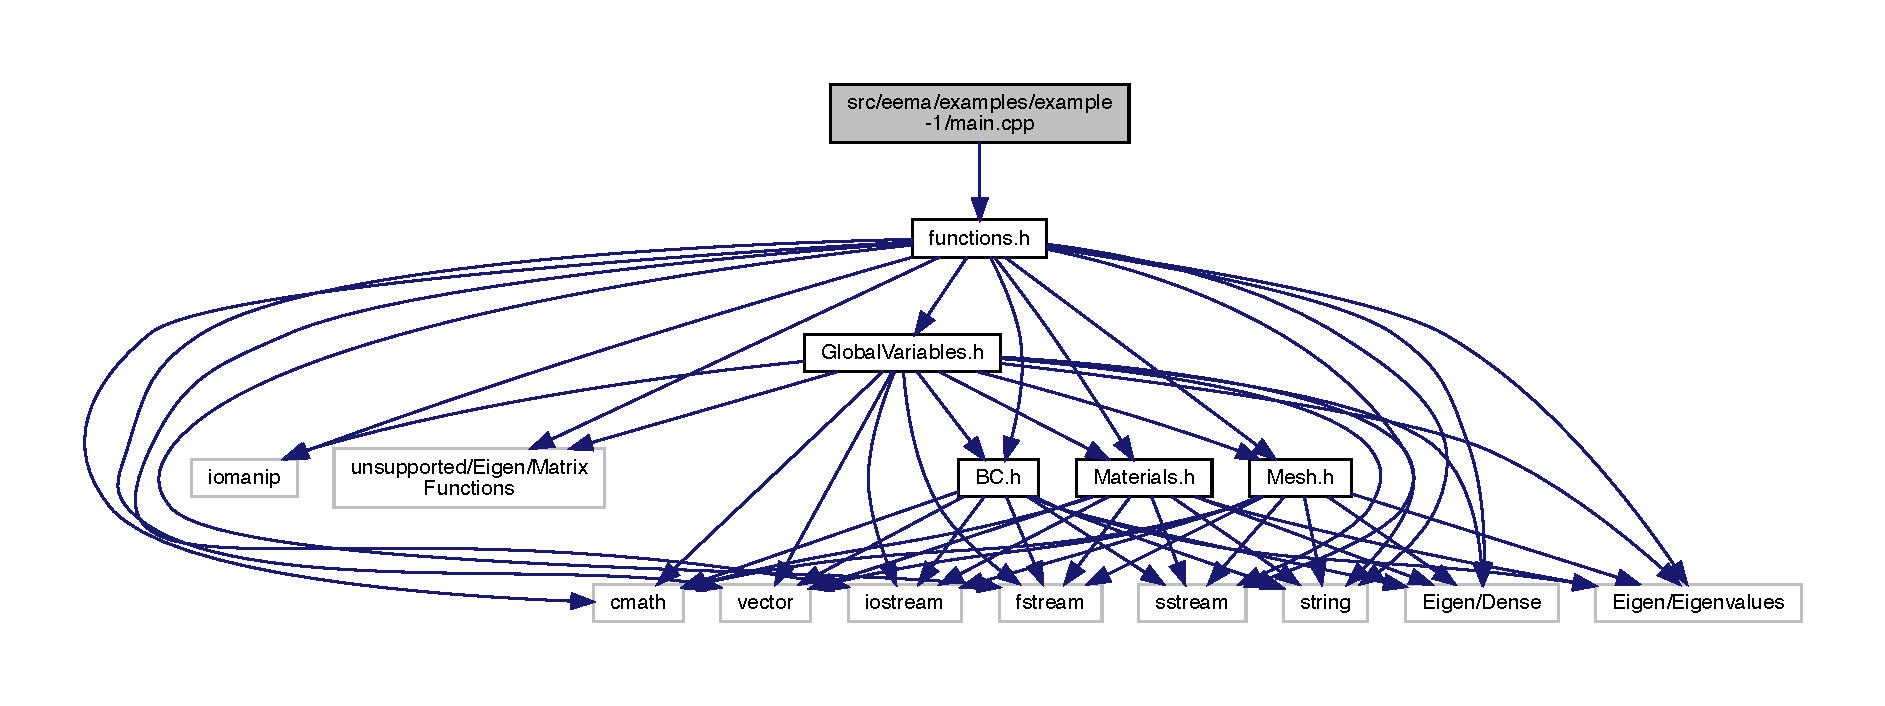
\includegraphics[width=350pt]{main_8cpp__incl}
\end{center}
\end{figure}
\subsection*{Functions}
\begin{DoxyCompactItemize}
\item 
int \hyperlink{main_8cpp_a3c04138a5bfe5d72780bb7e82a18e627}{main} (int argc, char $\ast$$\ast$argv)
\end{DoxyCompactItemize}


\subsection{Function Documentation}
\mbox{\Hypertarget{main_8cpp_a3c04138a5bfe5d72780bb7e82a18e627}\label{main_8cpp_a3c04138a5bfe5d72780bb7e82a18e627}} 
\index{main.\+cpp@{main.\+cpp}!main@{main}}
\index{main@{main}!main.\+cpp@{main.\+cpp}}
\subsubsection{\texorpdfstring{main()}{main()}}
{\footnotesize\ttfamily int main (\begin{DoxyParamCaption}\item[{int}]{argc,  }\item[{char $\ast$$\ast$}]{argv }\end{DoxyParamCaption})}

This is the main file. If you want to submit a new job -- this is where you do it Enter the path address for your job folder 

Definition at line \hyperlink{main_8cpp_source_l00006}{6} of file \hyperlink{main_8cpp_source}{main.\+cpp}.

Here is the call graph for this function\+:\nopagebreak
\begin{figure}[H]
\begin{center}
\leavevmode
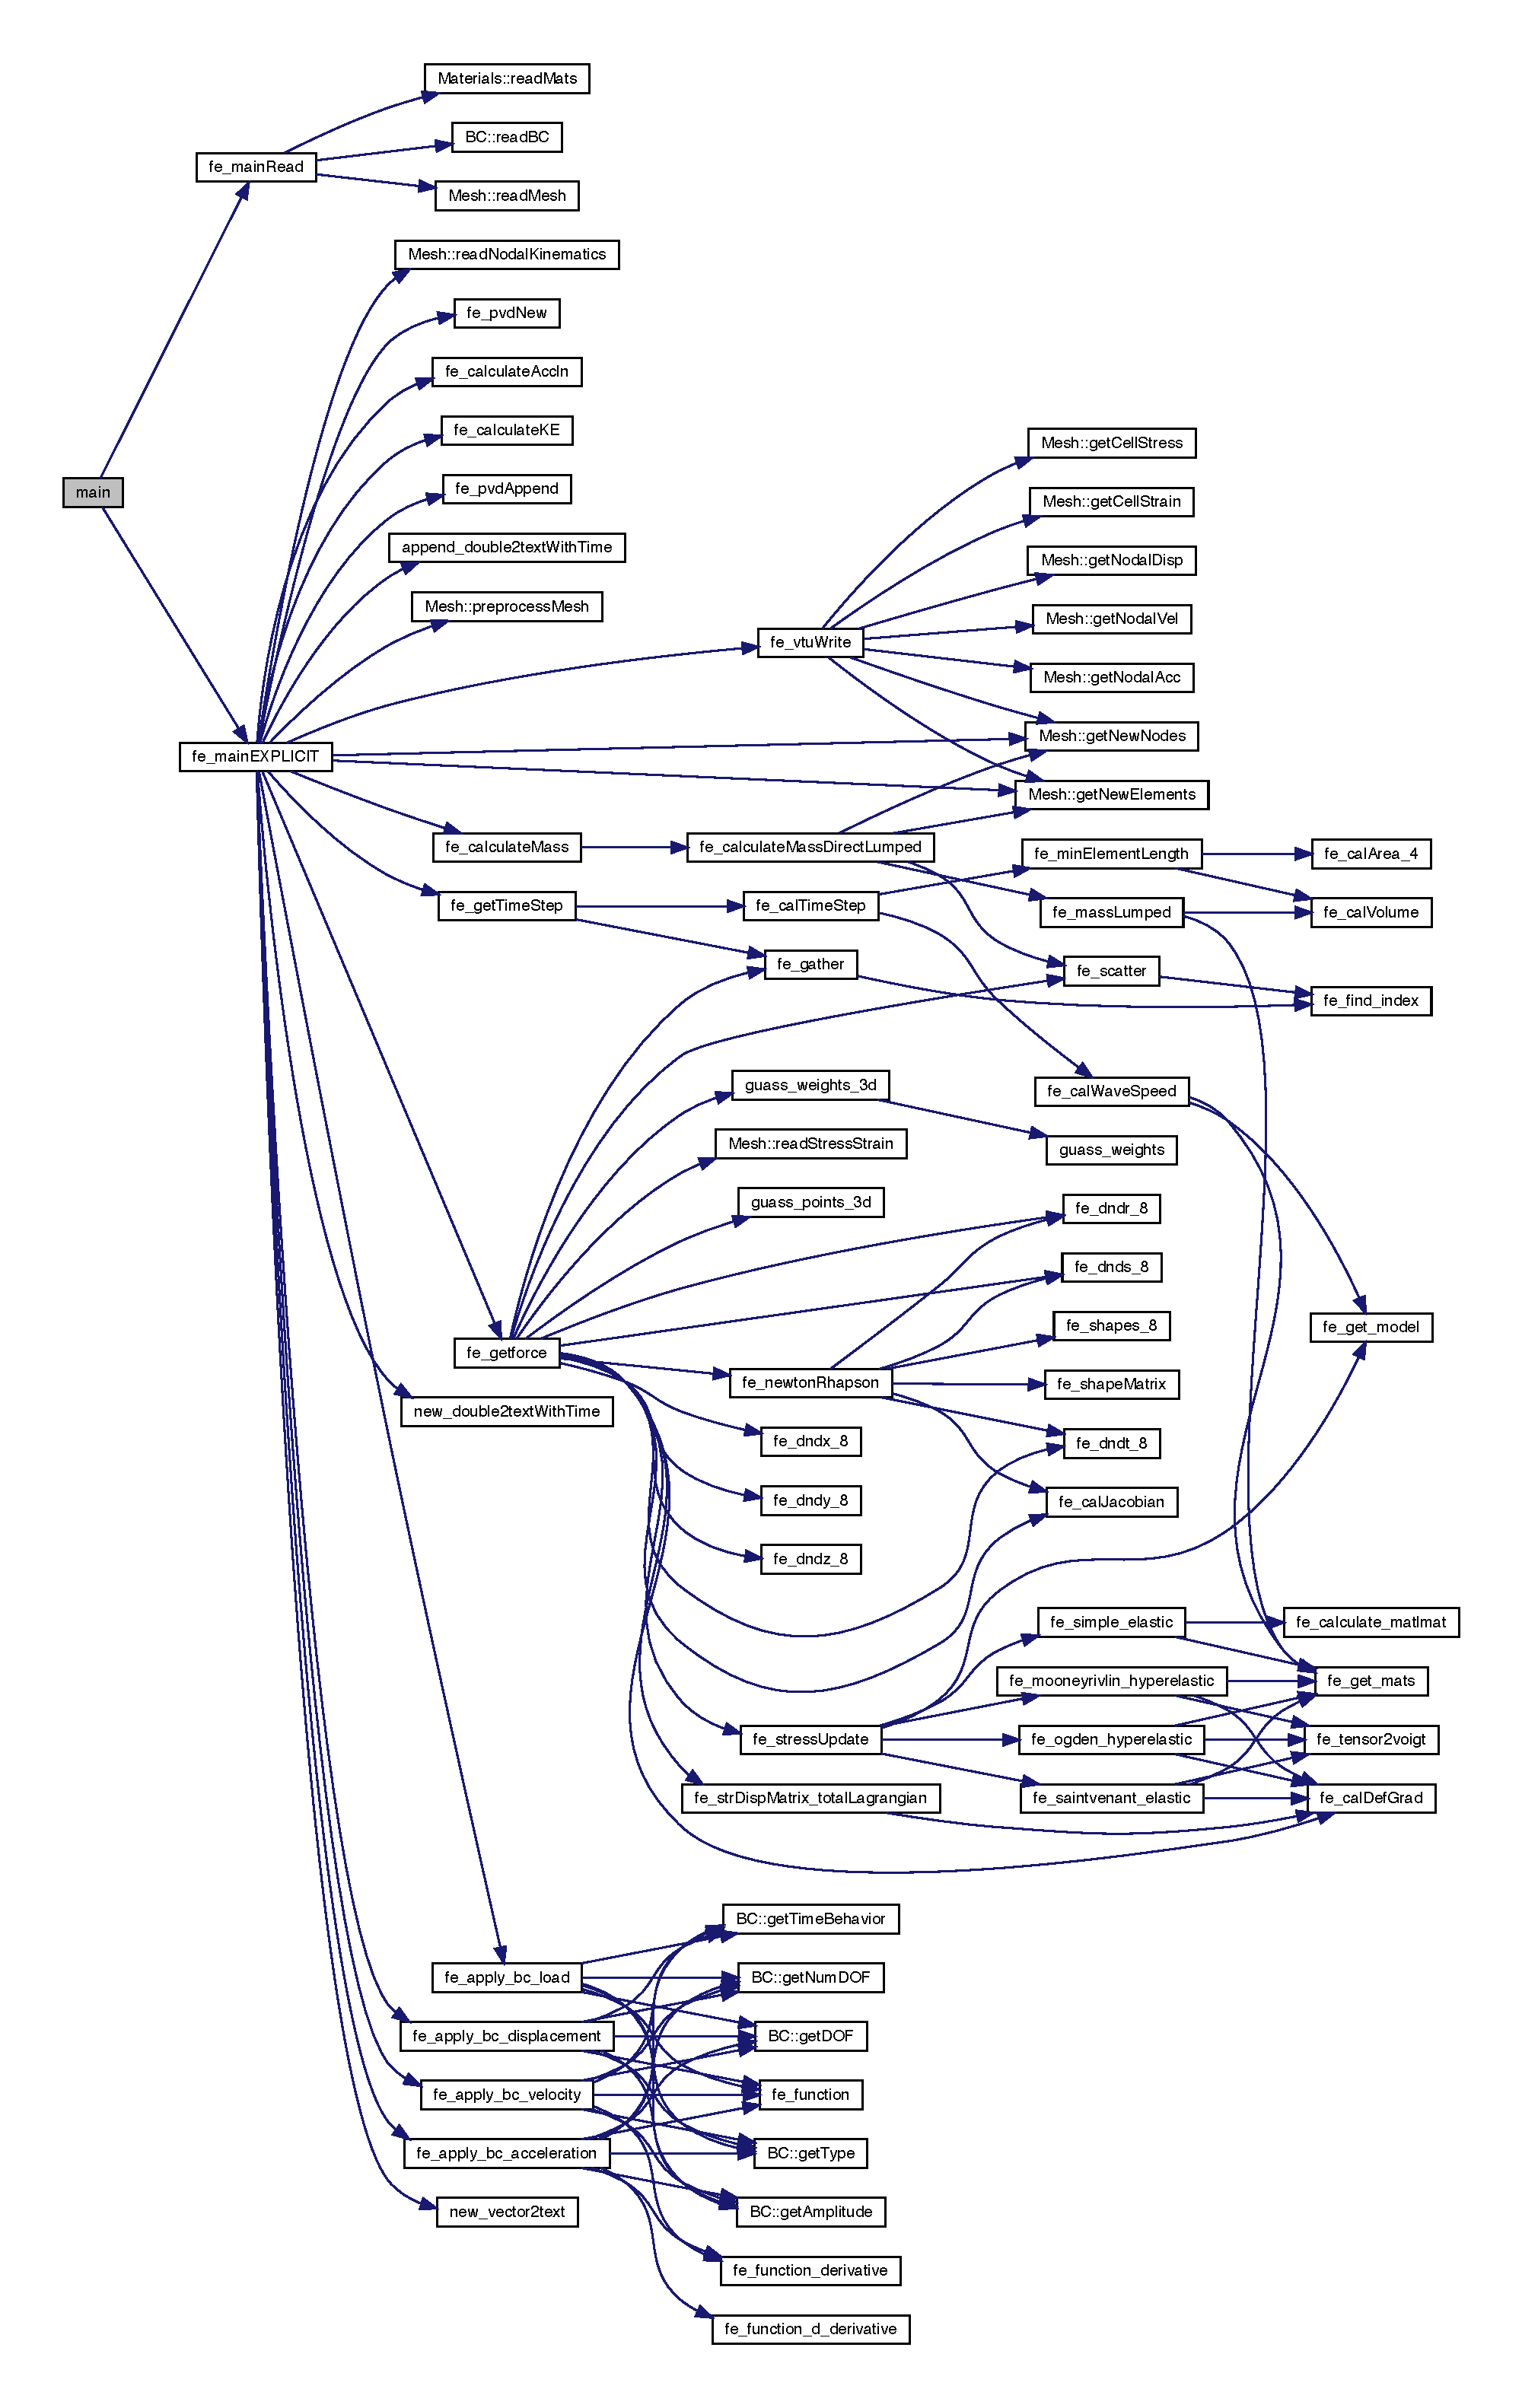
\includegraphics[height=550pt]{main_8cpp_a3c04138a5bfe5d72780bb7e82a18e627_cgraph}
\end{center}
\end{figure}

\hypertarget{main_8cpp_source}{}\section{main.\+cpp}
\label{main_8cpp_source}\index{src/eema/examples/example-\/1/main.\+cpp@{src/eema/examples/example-\/1/main.\+cpp}}

\begin{DoxyCode}
00001 \textcolor{preprocessor}{#include "\hyperlink{functions_8h}{functions.h}"}
00002 \textcolor{keyword}{using namespace }\hyperlink{namespace_eigen}{Eigen};
\Hypertarget{main_8cpp_source_l00006}\hyperlink{main_8cpp_a3c04138a5bfe5d72780bb7e82a18e627}{00006} \textcolor{keywordtype}{int} \hyperlink{main_8cpp_a3c04138a5bfe5d72780bb7e82a18e627}{main}(\textcolor{keywordtype}{int} argc, \textcolor{keywordtype}{char} **argv)\{
00007     clock\_t t;
00008     t = clock();
00009     
00011     \hyperlink{_global_variables_8h_a556ce46e457f991c51f3dac111579e2b}{home\_path} = argv[1];
00012     \hyperlink{_global_variables_8h_a5e3d7c3d50f127de0e61daaa407dc7d1}{job\_file} = argv[2];
00013 
00014     \hyperlink{functions_8h_a8a64e915e17f876fe72bedd820e87c33}{fe\_mainRead}(\hyperlink{_global_variables_8h_a556ce46e457f991c51f3dac111579e2b}{home\_path}+\textcolor{stringliteral}{"/"}+\hyperlink{_global_variables_8h_a5e3d7c3d50f127de0e61daaa407dc7d1}{job\_file});
00015     \hyperlink{functions_8h_ab2f8704631ca6c23a453d1905efbb162}{fe\_mainEXPLICIT}();
00016 
00017     t = clock()-t;
00018     std::cout<<\textcolor{stringliteral}{"--------------------------------------"}<<\textcolor{stringliteral}{"\(\backslash\)n"};
00019     std::cout<<\textcolor{stringliteral}{"Total Simulation CPU Time: "}<<(((float)t)/CLOCKS\_PER\_SEC)<<\textcolor{stringliteral}{"s \(\backslash\)n"};
00020     std::cout<<\textcolor{stringliteral}{"Simulation Completed."}<<\textcolor{stringliteral}{"\(\backslash\)n"};
00021     std::cout<<\textcolor{stringliteral}{"--------------------------------------"}<<\textcolor{stringliteral}{"\(\backslash\)n"};
00022     \textcolor{keywordflow}{return} 0;
00023 \}
\end{DoxyCode}

\hypertarget{_b_c_8h}{}\section{src/eema/include/\+BC.h File Reference}
\label{_b_c_8h}\index{src/eema/include/\+B\+C.\+h@{src/eema/include/\+B\+C.\+h}}
{\ttfamily \#include $<$iostream$>$}\newline
{\ttfamily \#include $<$cmath$>$}\newline
{\ttfamily \#include $<$vector$>$}\newline
{\ttfamily \#include $<$fstream$>$}\newline
{\ttfamily \#include $<$sstream$>$}\newline
{\ttfamily \#include $<$string$>$}\newline
{\ttfamily \#include \char`\"{}Eigen/\+Dense\char`\"{}}\newline
{\ttfamily \#include \char`\"{}Eigen/\+Eigenvalues\char`\"{}}\newline
Include dependency graph for B\+C.\+h\+:\nopagebreak
\begin{figure}[H]
\begin{center}
\leavevmode
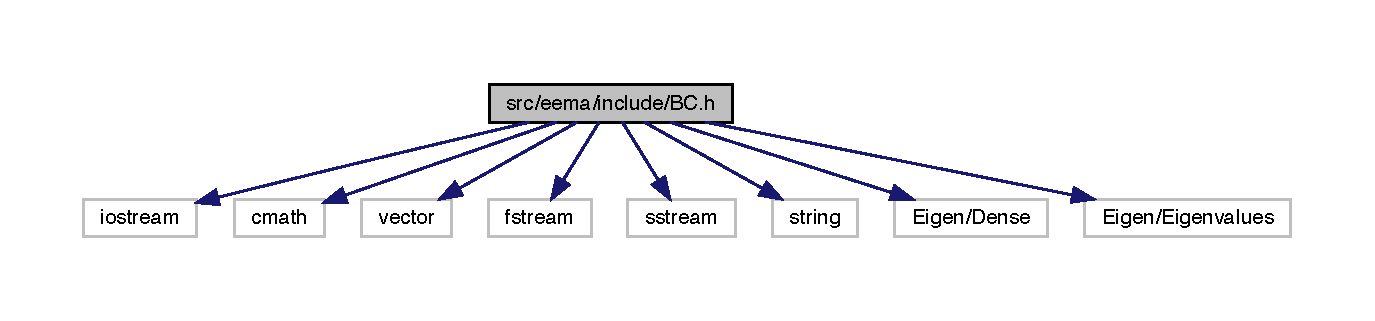
\includegraphics[width=350pt]{_b_c_8h__incl}
\end{center}
\end{figure}
This graph shows which files directly or indirectly include this file\+:\nopagebreak
\begin{figure}[H]
\begin{center}
\leavevmode

\includegraphics[width=350pt]{_b_c_8h__dep__incl}
\end{center}
\end{figure}
\subsection*{Classes}
\begin{DoxyCompactItemize}
\item 
class \hyperlink{class_b_c}{BC}
\end{DoxyCompactItemize}

\hypertarget{_b_c_8h_source}{}\section{B\+C.\+h}
\label{_b_c_8h_source}\index{src/eema/include/\+B\+C.\+h@{src/eema/include/\+B\+C.\+h}}

\begin{DoxyCode}
00001 \textcolor{preprocessor}{#ifndef HEADERS\_BC\_H\_}
00002 \textcolor{preprocessor}{#define HEADERS\_BC\_H\_}
00003 
00004 \textcolor{preprocessor}{#include<iostream>}
00005 \textcolor{preprocessor}{#include<cmath>}
00006 \textcolor{preprocessor}{#include<vector>}
00007 \textcolor{preprocessor}{#include<fstream>}
00008 \textcolor{preprocessor}{#include<sstream>}
00009 \textcolor{preprocessor}{#include<string>}
00010 
00011 \textcolor{preprocessor}{#include "Eigen/Dense"}
00012 \textcolor{preprocessor}{#include "Eigen/Eigenvalues"}
00013 
00014 \textcolor{keyword}{using namespace }\hyperlink{namespace_eigen}{Eigen};
00015 
\Hypertarget{_b_c_8h_source_l00016}\hyperlink{class_b_c}{00016} \textcolor{keyword}{class }\hyperlink{class_b_c}{BC}\{
00017 \textcolor{keyword}{private}:
\Hypertarget{_b_c_8h_source_l00018}\hyperlink{class_b_c_ab25297125dceec52f445a3a5efa77784}{00018}     std::string \hyperlink{class_b_c_ab25297125dceec52f445a3a5efa77784}{type};
\Hypertarget{_b_c_8h_source_l00019}\hyperlink{class_b_c_a25d7def8fdf5e988602759608b1507ea}{00019}     \textcolor{keywordtype}{double} \hyperlink{class_b_c_a25d7def8fdf5e988602759608b1507ea}{amplitude};
\Hypertarget{_b_c_8h_source_l00020}\hyperlink{class_b_c_a71fe2e36793286c4e683a3d8485abaf2}{00020}     \textcolor{keywordtype}{int} \hyperlink{class_b_c_a71fe2e36793286c4e683a3d8485abaf2}{num\_dof};
\Hypertarget{_b_c_8h_source_l00021}\hyperlink{class_b_c_a4e53c8862da8b017b419b201911d9e00}{00021}     VectorXi \hyperlink{class_b_c_a4e53c8862da8b017b419b201911d9e00}{dof};
\Hypertarget{_b_c_8h_source_l00022}\hyperlink{class_b_c_a84f989feaa5e81214f17b6dbdd1cf2ab}{00022}     std::string \hyperlink{class_b_c_a84f989feaa5e81214f17b6dbdd1cf2ab}{time\_curve};
00023 \textcolor{keyword}{public}:
00024     \textcolor{keywordtype}{void} readBC(std::string type\_user, \textcolor{keywordtype}{double} input\_amp\_user, \textcolor{keywordtype}{int} num\_dof\_user, VectorXi dof\_user, 
      std::string time\_curve\_user);
00025 
00026     std::string getType();
00027     \textcolor{keywordtype}{double} getAmplitude();
00028     \textcolor{keywordtype}{int} getNumDOF();
00029     VectorXi getDOF();
00030     std::string getTimeBehavior();
00031 
00032     \textcolor{keywordtype}{void} printBCInfo();
00033 \};
00034 
00035 \textcolor{preprocessor}{#endif }\textcolor{comment}{/* HEADERS\_BC\_H\_ */}\textcolor{preprocessor}{}
\end{DoxyCode}

\hypertarget{functions_8h}{}\section{src/eema/include/functions.h File Reference}
\label{functions_8h}\index{src/eema/include/functions.\+h@{src/eema/include/functions.\+h}}
{\ttfamily \#include $<$iostream$>$}\newline
{\ttfamily \#include $<$cmath$>$}\newline
{\ttfamily \#include $<$vector$>$}\newline
{\ttfamily \#include $<$fstream$>$}\newline
{\ttfamily \#include $<$sstream$>$}\newline
{\ttfamily \#include $<$string$>$}\newline
{\ttfamily \#include $<$iomanip$>$}\newline
{\ttfamily \#include \char`\"{}Eigen/\+Dense\char`\"{}}\newline
{\ttfamily \#include \char`\"{}Eigen/\+Eigenvalues\char`\"{}}\newline
{\ttfamily \#include \char`\"{}unsupported/\+Eigen/\+Matrix\+Functions\char`\"{}}\newline
{\ttfamily \#include \char`\"{}Mesh.\+h\char`\"{}}\newline
{\ttfamily \#include \char`\"{}Materials.\+h\char`\"{}}\newline
{\ttfamily \#include \char`\"{}B\+C.\+h\char`\"{}}\newline
{\ttfamily \#include \char`\"{}Global\+Variables.\+h\char`\"{}}\newline
Include dependency graph for functions.\+h\+:\nopagebreak
\begin{figure}[H]
\begin{center}
\leavevmode
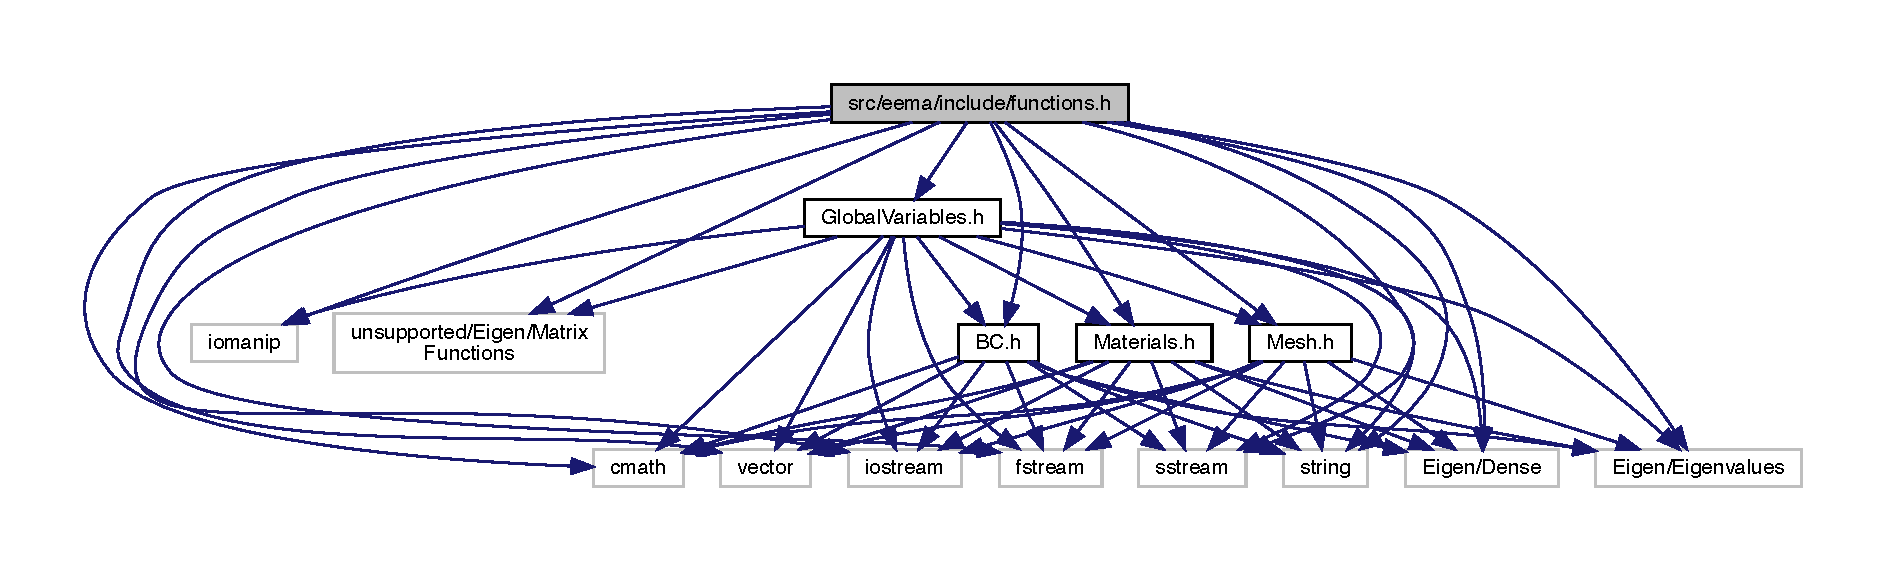
\includegraphics[width=350pt]{functions_8h__incl}
\end{center}
\end{figure}
This graph shows which files directly or indirectly include this file\+:\nopagebreak
\begin{figure}[H]
\begin{center}
\leavevmode

\includegraphics[width=350pt]{functions_8h__dep__incl}
\end{center}
\end{figure}
\subsection*{Functions}
\begin{DoxyCompactItemize}
\item 
Matrix\+Xd \hyperlink{functions_8h_add4fca63e194477644c3388febf88023}{text2matrix} (std\+::string name, int cols)
\item 
void \hyperlink{functions_8h_a346547477d2a1fbeff6b5e0b05314283}{matrix2text} (std\+::string name, Matrix\+Xd new\+\_\+slave\+\_\+master, int width)
\item 
void \hyperlink{functions_8h_a62d4a4906ace3f822fcebf7605c33c2b}{new\+\_\+vector2text} (std\+::string name, Vector\+Xd vector, int width)
\item 
void \hyperlink{functions_8h_aab8577bce9169902e0f328ddbc334cdc}{append\+\_\+double2text} (std\+::string name, double a)
\item 
void \hyperlink{functions_8h_a6908d3739a96b475c5f4c1623fad9316}{append\+\_\+double2text\+With\+Time} (std\+::string name, int frame, double time, double value)
\item 
void \hyperlink{functions_8h_ac861444df7684273e6c70504541eb892}{new\+\_\+double2text} (std\+::string name, double a)
\item 
void \hyperlink{functions_8h_ad1e19649d167234a1357071888353496}{new\+\_\+double2text\+With\+Time} (std\+::string name, int frame, double time, double value)
\item 
void \hyperlink{functions_8h_a9c39148b76d7691ea87e7f2f88b02295}{fe\+\_\+vtu\+Write} (std\+::string output, int time\+\_\+step, \hyperlink{class_mesh}{Mesh} mesh1)
\item 
void \hyperlink{functions_8h_aedbf95dc6f02a506b606328037cd58e1}{fe\+\_\+pvd\+New} (std\+::string output, int time\+\_\+step, double time)
\item 
void \hyperlink{functions_8h_ab350b9dfb65474874d79a92f712078a0}{fe\+\_\+pvd\+Append} (std\+::string output, int time\+\_\+step, double time)
\item 
void \hyperlink{functions_8h_a8a64e915e17f876fe72bedd820e87c33}{fe\+\_\+main\+Read} (std\+::string file)
\item 
Vector\+Xd \hyperlink{functions_8h_ab77a3a6d6f6b436d7e8c600bb0869927}{fe\+\_\+shapes\+\_\+8} (double rvalue, double svalue, double tvalue)
\item 
Vector\+Xd \hyperlink{functions_8h_afc547bef246c057db6cbd04bf7f866a9}{fe\+\_\+dndr\+\_\+8} (double rvalue, double svalue, double tvalue)
\item 
Vector\+Xd \hyperlink{functions_8h_ac0b5524525e1f2e89bb064c15ab8e664}{fe\+\_\+dnds\+\_\+8} (double rvalue, double svalue, double tvalue)
\item 
Vector\+Xd \hyperlink{functions_8h_a57e8e5c9f740c98e4767f29c121c2d0a}{fe\+\_\+dndt\+\_\+8} (double rvalue, double svalue, double tvalue)
\item 
Vector\+Xd \hyperlink{functions_8h_aa6ab8c3298fa10734e299fe8266aed35}{guass\+\_\+points} (int n)
\item 
Vector\+Xd \hyperlink{functions_8h_a84dcc9575e861bdb2872c10ba6238ee4}{guass\+\_\+weights} (int n)
\item 
Matrix\+Xd \hyperlink{functions_8h_a502e3469e1cc253deb142f46c0789a78}{guass\+\_\+points\+\_\+3d} (int nx, int ny, int nz)
\item 
Matrix\+Xd \hyperlink{functions_8h_ad99b08ce65ae353e91486d7685c22024}{guass\+\_\+weights\+\_\+3d} (int \hyperlink{fe__main_read_8cpp_aa789fe4d8a13fd0990b630909430d5d0}{ndof}, int nx, int ny, int nz)
\item 
Matrix\+Xd \hyperlink{functions_8h_a5ae3771e65b4a0d177097041a4349c28}{fe\+\_\+cal\+Jacobian} (int dim, int nnel, Vector\+Xd dndr, Vector\+Xd dnds, Vector\+Xd dndt, Vector\+Xd xcoord, Vector\+Xd ycoord, Vector\+Xd zcoord)
\item 
Vector\+Xd \hyperlink{functions_8h_afc6be1a5667e68156cb099e8da71170f}{fe\+\_\+dndx\+\_\+8} (int nnel, Vector\+Xd dndr, Vector\+Xd dnds, Vector\+Xd dndt, Matrix\+Xd inv\+Jacobian)
\item 
Vector\+Xd \hyperlink{functions_8h_a0572d7818e085c67f7fbb84eef8ecfb4}{fe\+\_\+dndy\+\_\+8} (int nnel, Vector\+Xd dndr, Vector\+Xd dnds, Vector\+Xd dndt, Matrix\+Xd inv\+Jacobian)
\item 
Vector\+Xd \hyperlink{functions_8h_aaf75db8433433807839c6ea17f2cf72c}{fe\+\_\+dndz\+\_\+8} (int nnel, Vector\+Xd dndr, Vector\+Xd dnds, Vector\+Xd dndt, Matrix\+Xd inv\+Jacobian)
\item 
Matrix\+Xd \hyperlink{functions_8h_a4b49d2df4f86e7d0755971ab4bfa48b2}{fe\+\_\+str\+Disp\+Matrix} (int edof, int nnel, Vector\+Xd dndx, Vector\+Xd dndy, Vector\+Xd dndz)
\item 
Matrix\+Xd \hyperlink{functions_8h_a98fae74dde5fe33a7062e7457a2d3227}{fe\+\_\+shape\+Matrix} (int edof, int nnel, Vector\+Xd shapes)
\item 
Matrix\+Xd \hyperlink{functions_8h_a0405e1196584e6fa36f29a2614a49f00}{fe\+\_\+mass\+\_\+hex} (Matrix\+Xd nodes, Vector\+Xi elements\+\_\+row)
\item 
Matrix\+Xd \hyperlink{functions_8h_a350d27ea0f1de929495d659b26f428d2}{fe\+\_\+mass\+\_\+truss} (double rho, double A\+\_\+truss, int edof, Matrix\+Xd nodes, Matrix\+Xd elements)
\item 
Matrix\+Xd \hyperlink{functions_8h_ab747d046148af042245ed13ca720c5ec}{fe\+\_\+transform\+Mass} (Matrix\+Xd m, int opt)
\item 
Matrix\+Xd \hyperlink{functions_8h_aa41c40dffea4251a07a8a3f5062f47ae}{fe\+\_\+cal\+Transformation} (Matrix\+Xd truss\+\_\+nodes, int choice)
\item 
Matrix\+Xd \hyperlink{functions_8h_ae2eeba997bf4f0bc4749b92130de7ba3}{fe\+\_\+cal\+Simp\+Transformation} (Matrix\+Xd truss\+\_\+nodes)
\item 
double \hyperlink{functions_8h_a6b04cfa4d2533eed9667ae14f361baa6}{fe\+\_\+min\+Element\+Length} (Vector\+Xd xcoord, Vector\+Xd ycoord, Vector\+Xd zcoord)
\item 
double \hyperlink{functions_8h_aa11bdbf370d88d267313624c85c28e70}{fe\+\_\+max\+Element\+Length} (Vector\+Xd xcoord, Vector\+Xd ycoord, Vector\+Xd zcoord)
\item 
Matrix\+Xd \hyperlink{functions_8h_a8c9fd519c93c847cdf52de947964eb67}{fe\+\_\+str\+Disp\+Matrix\+\_\+total\+Lagrangian} (int edof, int nnel, Vector\+Xd dndx, Vector\+Xd dndy, Vector\+Xd dndz, Vector\+Xd u)
\item 
Matrix\+Xd \hyperlink{functions_8h_ae50379f74802347e04dbc022897f9cb0}{fe\+\_\+cal\+Def\+Grad} (Vector\+Xd dndx, Vector\+Xd dndy, Vector\+Xd dndz, Vector\+Xd u)
\item 
Vector\+Xd \hyperlink{functions_8h_a73c4523ec7068af2af9e8431021f5fdf}{fe\+\_\+tensor2voigt} (Matrix\+Xd A)
\item 
Matrix\+Xd \hyperlink{functions_8h_a721a169d6a3d34b5584817ccd1c48cd7}{fe\+\_\+voigt2tensor} (Vector\+Xd B)
\item 
Matrix\+Xd \hyperlink{functions_8h_abbc5cafd6bb8048b69b3bd6f26ceb5f8}{fe\+\_\+calculate\+\_\+matlmat} (int n, double E, double nu)
\item 
Vector\+Xd \hyperlink{functions_8h_a7d0fd8cfef8b891901eb6f0f780fd9f2}{fe\+\_\+stress\+Update} (Vector\+Xd dndx, Vector\+Xd dndy, Vector\+Xd dndz, Matrix\+Xd disp\+\_\+mat, Vector\+Xd u, int opt, int return\+\_\+opt)
\begin{DoxyCompactList}\small\item\em This function calculates the updated stress for 3d elements -\/ elastic, hyperelastic material models were implemented so far. \end{DoxyCompactList}\item 
Vector\+Xd \hyperlink{functions_8h_a94c1b672863e28bc2c70d08726939929}{fe\+\_\+stress\+Update\+\_\+1d} (Vector\+Xd dndx, Vector\+Xd dndy, Vector\+Xd dndz, Vector\+Xd u\+\_\+e, int opt, Matrix\+Xd nodes)
\item 
double \hyperlink{functions_8h_af7ffbad6dfcc99fc88b130c1a7b1720a}{fe\+\_\+get\+\_\+mats} (int matl\+\_\+code, int obj\+\_\+interest)
\item 
std\+::string \hyperlink{functions_8h_a34d6fb85943d945b7e8600d2ef4220d0}{fe\+\_\+get\+\_\+model} (int matl\+\_\+code)
\item 
Vector\+Xd \hyperlink{functions_8h_a66b469439c736421744f6aef9e05a485}{fe\+\_\+mooneyrivlin\+\_\+hyperelastic} (Vector\+Xd dndx, Vector\+Xd dndy, Vector\+Xd dndz, Vector\+Xd u, int opt, int return\+\_\+opt)
\item 
Vector\+Xd \hyperlink{functions_8h_ab27ecb703db33cb21a8a6d2fbfbf125f}{fe\+\_\+ogden\+\_\+hyperelastic} (Vector\+Xd dndx, Vector\+Xd dndy, Vector\+Xd dndz, Vector\+Xd u, int opt, int return\+\_\+opt)
\item 
Vector\+Xd \hyperlink{functions_8h_ab0911abb05a0ca06eb4f330890ee0641}{fe\+\_\+simple\+\_\+elastic} (Vector\+Xd dndx, Vector\+Xd dndy, Vector\+Xd dndz, Matrix\+Xd disp\+\_\+mat, Vector\+Xd u, int opt, int return\+\_\+opt)
\item 
Vector\+Xd \hyperlink{functions_8h_af2a970e883d0c4a7ad750547c07c5f24}{fe\+\_\+saintvenant\+\_\+elastic} (Vector\+Xd dndx, Vector\+Xd dndy, Vector\+Xd dndz, Vector\+Xd u, int opt, int return\+\_\+opt)
\item 
double \hyperlink{functions_8h_ac1306a43db522f3da30471d2a6c48686}{fe\+\_\+cal\+Area\+\_\+4} (double a1, double a2, double a3, double a4, double b1, double b2, double b3, double b4, double c1, double c2, double c3, double c4)
\item 
double \hyperlink{functions_8h_a00f586c9a4bc56ec486776402fc26605}{fe\+\_\+cal\+Volume} (Vector\+Xd xcoord, Vector\+Xd ycoord, Vector\+Xd zcoord)
\item 
int \hyperlink{functions_8h_a983304137f9a961469a558437d5d2d59}{fe\+\_\+find} (Vector\+Xd A, double a)
\item 
int \hyperlink{functions_8h_a0d42c56d98efb23079057340a7133e89}{fe\+\_\+find} (Vector\+Xd A, int a)
\item 
Vector\+Xd \hyperlink{functions_8h_acdc9c3b5b3aecd9972c84d0cbb669978}{fe\+\_\+newton\+Rhapson} (Vector\+Xd nat\+\_\+coord, Vector\+Xd xcoord, Vector\+Xd ycoord, Vector\+Xd zcoord)
\begin{DoxyCompactList}\small\item\em This functions calculates the isoparametric coordinates of a set of coordinates in global system. \end{DoxyCompactList}\item 
double \hyperlink{functions_8h_a5ce8a3cf9dcc8b599ac40f7f3a48f196}{fe\+\_\+function} (double a, std\+::string b, double time)
\item 
double \hyperlink{functions_8h_aa587b020c768e2a11948bfd939829b6e}{fe\+\_\+function\+\_\+derivative} (double a, std\+::string b, double time)
\item 
double \hyperlink{functions_8h_afb02d53011656285452b16427dcd08dd}{fe\+\_\+function\+\_\+d\+\_\+derivative} (double a, std\+::string b, double time)
\item 
Matrix\+Xd \hyperlink{functions_8h_ac2d90cb6719488bc8551e6f9437f4f76}{fe\+\_\+concatenate\+\_\+vector2matrix} (Matrix\+Xd A, Vector\+Xd B, int opt)
\item 
Matrix\+Xd \hyperlink{functions_8h_a94d7770f842e44e01a47ae5624bd7749}{fe\+\_\+insert\+\_\+vector2matrix} (Matrix\+Xd A, Vector\+Xd B, int num, int opt)
\item 
Vector\+Xd \hyperlink{functions_8h_a6696827a8591495e5ea710b112fad5ef}{fe\+\_\+getforce} (Matrix\+Xd nodes, Matrix\+Xi elements, int \hyperlink{fe__main_read_8cpp_aa789fe4d8a13fd0990b630909430d5d0}{ndof}, Vector\+Xd u, Vector\+Xd v, Vector\+Xd fext, int size\+\_\+counter, Matrix\+Xd nodes\+\_\+truss, Matrix\+Xi elements\+\_\+truss)
\begin{DoxyCompactList}\small\item\em Calculates the resultant nodal force after each time step. \end{DoxyCompactList}\item 
Vector\+Xi \hyperlink{functions_8h_ae4dbe24b761cafa3577afab76726b382}{fe\+\_\+find\+\_\+index} (Vector\+Xi node\+\_\+list)
\item 
void \hyperlink{functions_8h_ab2f8704631ca6c23a453d1905efbb162}{fe\+\_\+main\+E\+X\+P\+L\+I\+C\+IT} ()
\begin{DoxyCompactList}\small\item\em This function carries out the explicit dynamic analysis of the F\+EM problem. \end{DoxyCompactList}\item 
Vector\+Xd \hyperlink{functions_8h_af42938e5b32edb33ef4a35866949eba6}{fe\+\_\+apply\+\_\+bc\+\_\+displacement} (Vector\+Xd U, double time)
\item 
Vector\+Xd \hyperlink{functions_8h_a4627586ca0e6b9e3904cdbc7bb561e9e}{fe\+\_\+apply\+\_\+bc\+\_\+velocity} (Vector\+Xd V, double time)
\item 
Vector\+Xd \hyperlink{functions_8h_ac0ffd5f19ac286c91d431a4ec72dbab4}{fe\+\_\+apply\+\_\+bc\+\_\+acceleration} (Vector\+Xd A, double time)
\item 
Vector\+Xd \hyperlink{functions_8h_aba32cc24bd74a4965c560fa62c5b213e}{fe\+\_\+apply\+\_\+bc\+\_\+load} (Vector\+Xd fe, double time)
\item 
Matrix\+Xd \hyperlink{functions_8h_a04f569c566ca4fbea3b3a2a13cdd0af5}{fe\+\_\+assemble\+\_\+mass} (Matrix\+Xd mm, Matrix\+Xd m, Vector\+Xi node\+\_\+list, int sdof)
\item 
Vector\+Xd \hyperlink{functions_8h_ab5053cb12ac67971a7836346e2839725}{fe\+\_\+gather} (Vector\+Xd global\+\_\+vec, Vector\+Xd local\+\_\+vec, Vector\+Xi node\+\_\+list, int sdof)
\item 
Vector\+Xd \hyperlink{functions_8h_a6b8344e12f9005795f93f60ddda26c5c}{fe\+\_\+scatter} (Vector\+Xd global\+\_\+vec, Vector\+Xd local\+\_\+vec, Vector\+Xi node\+\_\+list, int sdof)
\item 
Matrix\+Xd \hyperlink{functions_8h_a81ce693c4400df82b8753f25cc2dcabc}{fe\+\_\+update\+Nodes} (Matrix\+Xd nodes, Vector\+Xd displacements)
\item 
Vector\+Xd \hyperlink{functions_8h_a0600721e5cf84d84408ce9605b004610}{fe\+\_\+embed\+\_\+preprocessing\+\_\+mapping} (\hyperlink{class_mesh}{Mesh} host, \hyperlink{class_mesh}{Mesh} embed)
\item 
Vector\+Xd \hyperlink{functions_8h_a840ddc7df1916f6b5dfbb141adac32d3}{fe\+\_\+embed\+\_\+preprocessing} (\hyperlink{class_mesh}{Mesh} host, \hyperlink{class_mesh}{Mesh} embed)
\item 
void \hyperlink{functions_8h_a50e8d7839525058d40e3a53f9d5de77c}{fe\+\_\+embed\+\_\+preprocessing\+\_\+length} (\hyperlink{class_mesh}{Mesh} host, \hyperlink{class_mesh}{Mesh} embed)
\item 
int \hyperlink{functions_8h_a453ba6bc1e7d5a63db9d56beb6077a27}{fe\+\_\+compute\+\_\+host} (Vector\+Xd A, Matrix\+Xd nodes\+\_\+host, Matrix\+Xd elements\+\_\+host\+\_\+tmp)
\item 
Matrix\+Xd \hyperlink{functions_8h_a150d77644eb280d58564e3ff4885e73c}{fe\+\_\+create\+\_\+bbox} (Vector\+Xd A, Matrix\+Xd nodes\+\_\+host, Matrix\+Xd elements\+\_\+host, double length)
\item 
double \hyperlink{functions_8h_a20aed1a2d3d8b470592491a96e60be87}{fe\+\_\+cal\+Wave\+Speed} (int material\+\_\+id)
\item 
double \hyperlink{functions_8h_a537640b537f4b485607b062f2c25d974}{fe\+\_\+get\+Time\+Step} (Matrix\+Xd nodes, Matrix\+Xi elements, int \hyperlink{fe__main_read_8cpp_aa789fe4d8a13fd0990b630909430d5d0}{ndof}, Vector\+Xd u, Vector\+Xd v, Vector\+Xd fext)
\item 
double \hyperlink{functions_8h_a295b08cc71d5af080f0450614a01a4e6}{fe\+\_\+cal\+Time\+Step} (Vector\+Xd xcoord, Vector\+Xd ycoord, Vector\+Xd zcoord, int material\+\_\+id)
\item 
void \hyperlink{functions_8h_ae02497eb9e23d26212b7a1301fc5b04b}{fe\+\_\+vtk\+Write\+\_\+host} (std\+::string output, int format\+\_\+choice, int mesh\+\_\+choice, int time\+\_\+step, Matrix\+Xd nodes, Matrix\+Xi elements)
\item 
void \hyperlink{functions_8h_a35bde18dc6d9d842ff0bec995327d441}{fe\+\_\+vtk\+Write\+\_\+truss} (std\+::string output, int format\+\_\+choice, int mesh\+\_\+choice, int time\+\_\+step, Matrix\+Xd nodes, Matrix\+Xi elements)
\item 
void \hyperlink{functions_8h_ab3e39c6d01b6fd10c9e264731cef75dc}{fe\+\_\+display\+\_\+vector} (Vector\+Xd A)
\item 
void \hyperlink{functions_8h_a5110a192d089c6b26744b9e9d67a7c2d}{fe\+\_\+display\+\_\+matrix} (Matrix\+Xd A)
\item 
Matrix\+Xd \hyperlink{functions_8h_a3c73fda948017ac96aeb19889cfc1cba}{fe\+\_\+apply\+\_\+bc\+\_\+stiffness} (Matrix\+Xd kk, Vector\+Xi bcdof, Vector\+Xd bcval)
\item 
Matrix\+Xd \hyperlink{functions_8h_a9378d4fc517465015411134456235a76}{fe\+\_\+stiffness\+\_\+hex} (double E, double nu, int \hyperlink{fe__main_read_8cpp_aa789fe4d8a13fd0990b630909430d5d0}{ndof}, int nnel, int edof, double xcoord\mbox{[}$\,$\mbox{]}, double ycoord\mbox{[}$\,$\mbox{]}, double zcoord\mbox{[}$\,$\mbox{]})
\item 
Matrix\+Xd \hyperlink{functions_8h_ab3798340a27f0972299b3820aab0ccba}{fe\+\_\+stiffness\+\_\+embed\+\_\+truss} (Matrix\+Xd nodes\+\_\+truss, Matrix\+Xd elements\+\_\+truss, double E\+\_\+truss, double A\+\_\+truss, int \hyperlink{fe__main_read_8cpp_aa789fe4d8a13fd0990b630909430d5d0}{ndof}, int nnel, int edof, double xcoord\mbox{[}$\,$\mbox{]}, double ycoord\mbox{[}$\,$\mbox{]}, double zcoord\mbox{[}$\,$\mbox{]})
\item 
void \hyperlink{functions_8h_a9dec90c41460e15aa1d8dce787683406}{fe\+\_\+write\+Element\+Stress} (Matrix\+Xd sigma\+\_\+all, double time)
\item 
Vector\+Xd \hyperlink{functions_8h_abeed10bd80ae1f3c95d79c4aed512d8f}{fe\+\_\+calculate\+Mass} (Vector\+Xd mm, std\+::string type)
\item 
Vector\+Xd \hyperlink{functions_8h_aca6d101baf8887cf61064067985cbd62}{fe\+\_\+calculate\+Mass\+Direct\+Lumped} (Vector\+Xd mm)
\item 
Vector\+Xd \hyperlink{functions_8h_aa34a87447bf9fa851463ce99101a7054}{fe\+\_\+mass\+Lumped} (Matrix\+Xd nodes, Vector\+Xi elements\+\_\+row)
\item 
Vector\+Xd \hyperlink{functions_8h_a049ed85fefb5b5e80e42432fdcc640fa}{fe\+\_\+calculate\+Accln} (Vector\+Xd mm, Vector\+Xd F\+\_\+net)
\item 
double \hyperlink{functions_8h_afb8a8298008daf8f2e705a9acb72b984}{fe\+\_\+calculate\+KE} (Vector\+Xd mm, Vector\+Xd V)
\item 
double \hyperlink{functions_8h_a0bdf25bf63fdb63302feaecb1284626e}{fe\+\_\+calculate\+KE} (Matrix\+Xd mm, Vector\+Xd V)
\item 
Vector\+Xd \hyperlink{functions_8h_a708d7eae199de06b3c6627cc90bf569e}{text2vector} (std\+::string name)
\end{DoxyCompactItemize}


\subsection{Function Documentation}
\mbox{\Hypertarget{functions_8h_aab8577bce9169902e0f328ddbc334cdc}\label{functions_8h_aab8577bce9169902e0f328ddbc334cdc}} 
\index{functions.\+h@{functions.\+h}!append\+\_\+double2text@{append\+\_\+double2text}}
\index{append\+\_\+double2text@{append\+\_\+double2text}!functions.\+h@{functions.\+h}}
\subsubsection{\texorpdfstring{append\+\_\+double2text()}{append\_double2text()}}
{\footnotesize\ttfamily void append\+\_\+double2text (\begin{DoxyParamCaption}\item[{std\+::string}]{name,  }\item[{double}]{a }\end{DoxyParamCaption})}

Function appends a double value to a text file 

Definition at line \hyperlink{fe__vector2text_8cpp_source_l00017}{17} of file \hyperlink{fe__vector2text_8cpp_source}{fe\+\_\+vector2text.\+cpp}.

\mbox{\Hypertarget{functions_8h_a6908d3739a96b475c5f4c1623fad9316}\label{functions_8h_a6908d3739a96b475c5f4c1623fad9316}} 
\index{functions.\+h@{functions.\+h}!append\+\_\+double2text\+With\+Time@{append\+\_\+double2text\+With\+Time}}
\index{append\+\_\+double2text\+With\+Time@{append\+\_\+double2text\+With\+Time}!functions.\+h@{functions.\+h}}
\subsubsection{\texorpdfstring{append\+\_\+double2text\+With\+Time()}{append\_double2textWithTime()}}
{\footnotesize\ttfamily void append\+\_\+double2text\+With\+Time (\begin{DoxyParamCaption}\item[{std\+::string}]{name,  }\item[{int}]{frame,  }\item[{double}]{time,  }\item[{double}]{value }\end{DoxyParamCaption})}

Function appends a double value with solution times to a text file 

Definition at line \hyperlink{fe__vector2text_8cpp_source_l00028}{28} of file \hyperlink{fe__vector2text_8cpp_source}{fe\+\_\+vector2text.\+cpp}.

Here is the caller graph for this function\+:\nopagebreak
\begin{figure}[H]
\begin{center}
\leavevmode
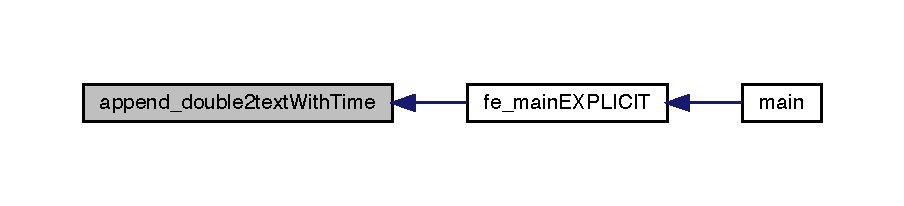
\includegraphics[width=350pt]{functions_8h_a6908d3739a96b475c5f4c1623fad9316_icgraph}
\end{center}
\end{figure}
\mbox{\Hypertarget{functions_8h_ac0ffd5f19ac286c91d431a4ec72dbab4}\label{functions_8h_ac0ffd5f19ac286c91d431a4ec72dbab4}} 
\index{functions.\+h@{functions.\+h}!fe\+\_\+apply\+\_\+bc\+\_\+acceleration@{fe\+\_\+apply\+\_\+bc\+\_\+acceleration}}
\index{fe\+\_\+apply\+\_\+bc\+\_\+acceleration@{fe\+\_\+apply\+\_\+bc\+\_\+acceleration}!functions.\+h@{functions.\+h}}
\subsubsection{\texorpdfstring{fe\+\_\+apply\+\_\+bc\+\_\+acceleration()}{fe\_apply\_bc\_acceleration()}}
{\footnotesize\ttfamily Vector\+Xd fe\+\_\+apply\+\_\+bc\+\_\+acceleration (\begin{DoxyParamCaption}\item[{Vector\+Xd}]{A,  }\item[{double}]{time }\end{DoxyParamCaption})}

Function enforces acceleration boundary condition 

Definition at line \hyperlink{fe__apply__bc_8cpp_source_l00056}{56} of file \hyperlink{fe__apply__bc_8cpp_source}{fe\+\_\+apply\+\_\+bc.\+cpp}.

Here is the call graph for this function\+:\nopagebreak
\begin{figure}[H]
\begin{center}
\leavevmode
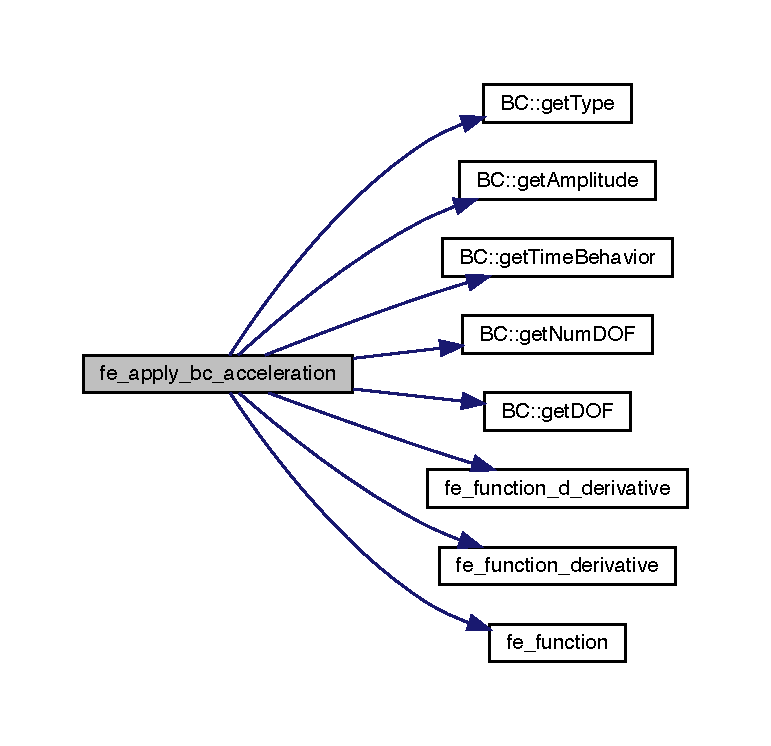
\includegraphics[width=350pt]{functions_8h_ac0ffd5f19ac286c91d431a4ec72dbab4_cgraph}
\end{center}
\end{figure}
Here is the caller graph for this function\+:\nopagebreak
\begin{figure}[H]
\begin{center}
\leavevmode
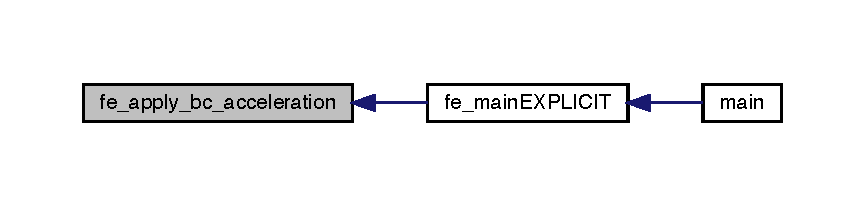
\includegraphics[width=350pt]{functions_8h_ac0ffd5f19ac286c91d431a4ec72dbab4_icgraph}
\end{center}
\end{figure}
\mbox{\Hypertarget{functions_8h_af42938e5b32edb33ef4a35866949eba6}\label{functions_8h_af42938e5b32edb33ef4a35866949eba6}} 
\index{functions.\+h@{functions.\+h}!fe\+\_\+apply\+\_\+bc\+\_\+displacement@{fe\+\_\+apply\+\_\+bc\+\_\+displacement}}
\index{fe\+\_\+apply\+\_\+bc\+\_\+displacement@{fe\+\_\+apply\+\_\+bc\+\_\+displacement}!functions.\+h@{functions.\+h}}
\subsubsection{\texorpdfstring{fe\+\_\+apply\+\_\+bc\+\_\+displacement()}{fe\_apply\_bc\_displacement()}}
{\footnotesize\ttfamily Vector\+Xd fe\+\_\+apply\+\_\+bc\+\_\+displacement (\begin{DoxyParamCaption}\item[{Vector\+Xd}]{U,  }\item[{double}]{time }\end{DoxyParamCaption})}

Function enforces displacement boundary condition 

Definition at line \hyperlink{fe__apply__bc_8cpp_source_l00005}{5} of file \hyperlink{fe__apply__bc_8cpp_source}{fe\+\_\+apply\+\_\+bc.\+cpp}.

Here is the call graph for this function\+:\nopagebreak
\begin{figure}[H]
\begin{center}
\leavevmode
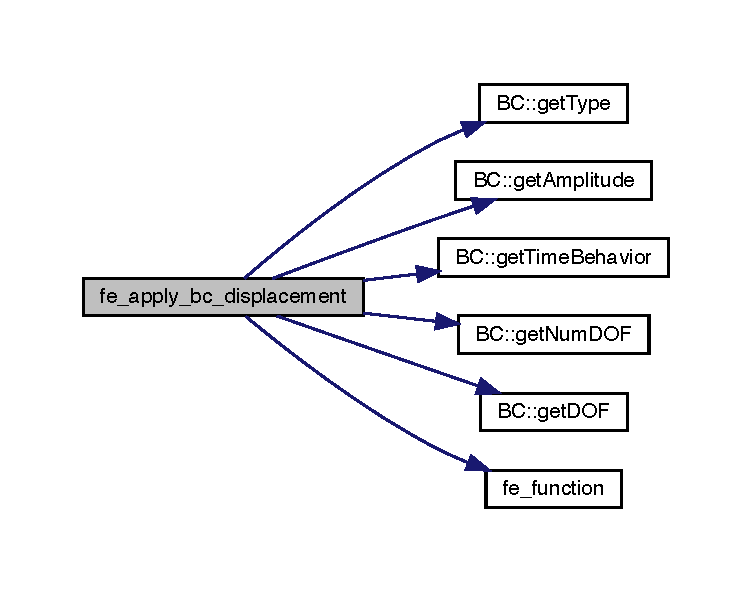
\includegraphics[width=350pt]{functions_8h_af42938e5b32edb33ef4a35866949eba6_cgraph}
\end{center}
\end{figure}
Here is the caller graph for this function\+:\nopagebreak
\begin{figure}[H]
\begin{center}
\leavevmode
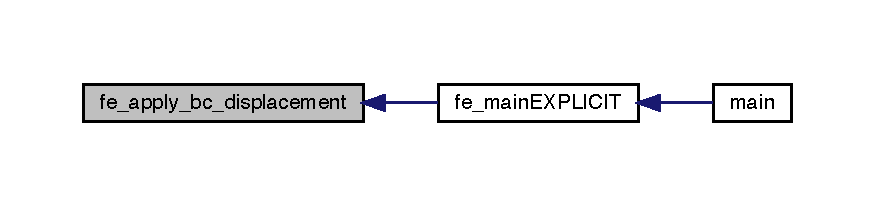
\includegraphics[width=350pt]{functions_8h_af42938e5b32edb33ef4a35866949eba6_icgraph}
\end{center}
\end{figure}
\mbox{\Hypertarget{functions_8h_aba32cc24bd74a4965c560fa62c5b213e}\label{functions_8h_aba32cc24bd74a4965c560fa62c5b213e}} 
\index{functions.\+h@{functions.\+h}!fe\+\_\+apply\+\_\+bc\+\_\+load@{fe\+\_\+apply\+\_\+bc\+\_\+load}}
\index{fe\+\_\+apply\+\_\+bc\+\_\+load@{fe\+\_\+apply\+\_\+bc\+\_\+load}!functions.\+h@{functions.\+h}}
\subsubsection{\texorpdfstring{fe\+\_\+apply\+\_\+bc\+\_\+load()}{fe\_apply\_bc\_load()}}
{\footnotesize\ttfamily Vector\+Xd fe\+\_\+apply\+\_\+bc\+\_\+load (\begin{DoxyParamCaption}\item[{Vector\+Xd}]{fe,  }\item[{double}]{time }\end{DoxyParamCaption})}

Function updates the applied load 

Definition at line \hyperlink{fe__apply__bc_8cpp_source_l00099}{99} of file \hyperlink{fe__apply__bc_8cpp_source}{fe\+\_\+apply\+\_\+bc.\+cpp}.

Here is the call graph for this function\+:\nopagebreak
\begin{figure}[H]
\begin{center}
\leavevmode
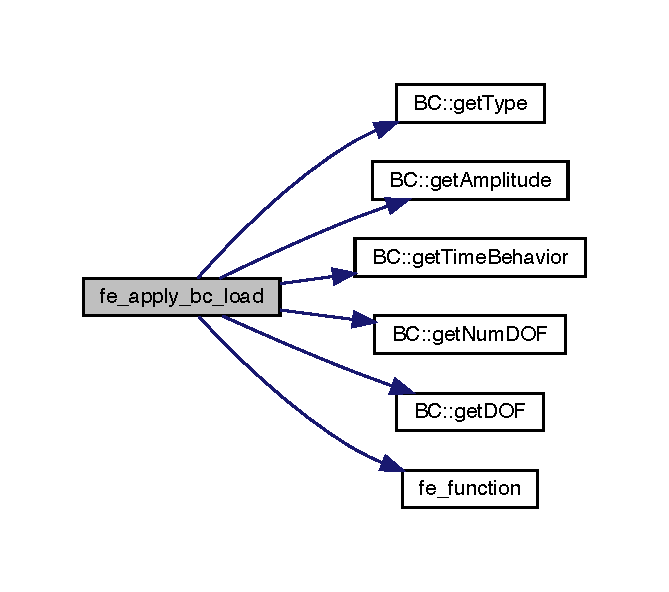
\includegraphics[width=321pt]{functions_8h_aba32cc24bd74a4965c560fa62c5b213e_cgraph}
\end{center}
\end{figure}
Here is the caller graph for this function\+:\nopagebreak
\begin{figure}[H]
\begin{center}
\leavevmode
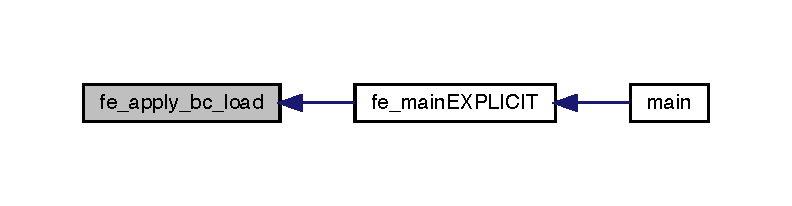
\includegraphics[width=350pt]{functions_8h_aba32cc24bd74a4965c560fa62c5b213e_icgraph}
\end{center}
\end{figure}
\mbox{\Hypertarget{functions_8h_a3c73fda948017ac96aeb19889cfc1cba}\label{functions_8h_a3c73fda948017ac96aeb19889cfc1cba}} 
\index{functions.\+h@{functions.\+h}!fe\+\_\+apply\+\_\+bc\+\_\+stiffness@{fe\+\_\+apply\+\_\+bc\+\_\+stiffness}}
\index{fe\+\_\+apply\+\_\+bc\+\_\+stiffness@{fe\+\_\+apply\+\_\+bc\+\_\+stiffness}!functions.\+h@{functions.\+h}}
\subsubsection{\texorpdfstring{fe\+\_\+apply\+\_\+bc\+\_\+stiffness()}{fe\_apply\_bc\_stiffness()}}
{\footnotesize\ttfamily Matrix\+Xd fe\+\_\+apply\+\_\+bc\+\_\+stiffness (\begin{DoxyParamCaption}\item[{Matrix\+Xd}]{kk,  }\item[{Vector\+Xi}]{bcdof,  }\item[{Vector\+Xd}]{bcval }\end{DoxyParamCaption})}



Definition at line \hyperlink{fe__apply__bc_8cpp_source_l00118}{118} of file \hyperlink{fe__apply__bc_8cpp_source}{fe\+\_\+apply\+\_\+bc.\+cpp}.

\mbox{\Hypertarget{functions_8h_a4627586ca0e6b9e3904cdbc7bb561e9e}\label{functions_8h_a4627586ca0e6b9e3904cdbc7bb561e9e}} 
\index{functions.\+h@{functions.\+h}!fe\+\_\+apply\+\_\+bc\+\_\+velocity@{fe\+\_\+apply\+\_\+bc\+\_\+velocity}}
\index{fe\+\_\+apply\+\_\+bc\+\_\+velocity@{fe\+\_\+apply\+\_\+bc\+\_\+velocity}!functions.\+h@{functions.\+h}}
\subsubsection{\texorpdfstring{fe\+\_\+apply\+\_\+bc\+\_\+velocity()}{fe\_apply\_bc\_velocity()}}
{\footnotesize\ttfamily Vector\+Xd fe\+\_\+apply\+\_\+bc\+\_\+velocity (\begin{DoxyParamCaption}\item[{Vector\+Xd}]{V,  }\item[{double}]{time }\end{DoxyParamCaption})}

Function enforces velocity boundary condition 

Definition at line \hyperlink{fe__apply__bc_8cpp_source_l00024}{24} of file \hyperlink{fe__apply__bc_8cpp_source}{fe\+\_\+apply\+\_\+bc.\+cpp}.

Here is the call graph for this function\+:\nopagebreak
\begin{figure}[H]
\begin{center}
\leavevmode
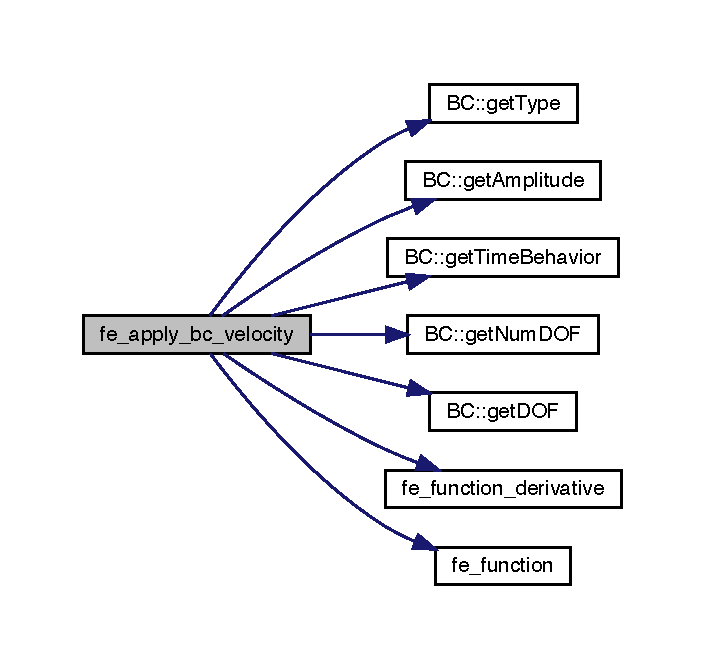
\includegraphics[width=338pt]{functions_8h_a4627586ca0e6b9e3904cdbc7bb561e9e_cgraph}
\end{center}
\end{figure}
Here is the caller graph for this function\+:\nopagebreak
\begin{figure}[H]
\begin{center}
\leavevmode
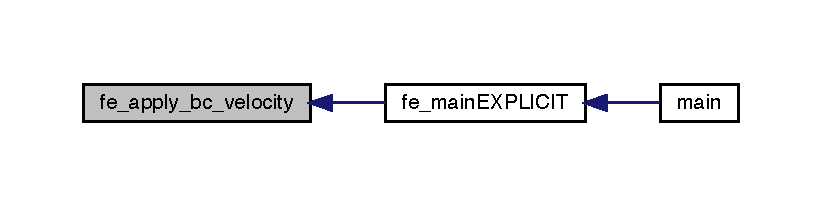
\includegraphics[width=350pt]{functions_8h_a4627586ca0e6b9e3904cdbc7bb561e9e_icgraph}
\end{center}
\end{figure}
\mbox{\Hypertarget{functions_8h_a04f569c566ca4fbea3b3a2a13cdd0af5}\label{functions_8h_a04f569c566ca4fbea3b3a2a13cdd0af5}} 
\index{functions.\+h@{functions.\+h}!fe\+\_\+assemble\+\_\+mass@{fe\+\_\+assemble\+\_\+mass}}
\index{fe\+\_\+assemble\+\_\+mass@{fe\+\_\+assemble\+\_\+mass}!functions.\+h@{functions.\+h}}
\subsubsection{\texorpdfstring{fe\+\_\+assemble\+\_\+mass()}{fe\_assemble\_mass()}}
{\footnotesize\ttfamily Matrix\+Xd fe\+\_\+assemble\+\_\+mass (\begin{DoxyParamCaption}\item[{Matrix\+Xd}]{mm,  }\item[{Matrix\+Xd}]{m,  }\item[{Vector\+Xi}]{node\+\_\+list,  }\item[{int}]{sdof }\end{DoxyParamCaption})}

Assembles the global mass matrix 

Definition at line \hyperlink{fe__assemble__mass_8cpp_source_l00024}{24} of file \hyperlink{fe__assemble__mass_8cpp_source}{fe\+\_\+assemble\+\_\+mass.\+cpp}.

Here is the call graph for this function\+:\nopagebreak
\begin{figure}[H]
\begin{center}
\leavevmode
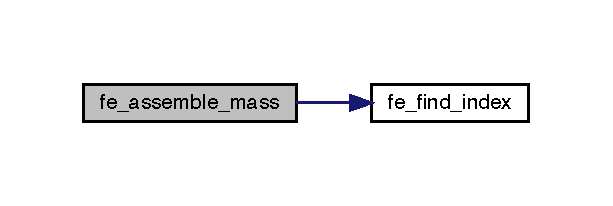
\includegraphics[width=294pt]{functions_8h_a04f569c566ca4fbea3b3a2a13cdd0af5_cgraph}
\end{center}
\end{figure}
\mbox{\Hypertarget{functions_8h_ac1306a43db522f3da30471d2a6c48686}\label{functions_8h_ac1306a43db522f3da30471d2a6c48686}} 
\index{functions.\+h@{functions.\+h}!fe\+\_\+cal\+Area\+\_\+4@{fe\+\_\+cal\+Area\+\_\+4}}
\index{fe\+\_\+cal\+Area\+\_\+4@{fe\+\_\+cal\+Area\+\_\+4}!functions.\+h@{functions.\+h}}
\subsubsection{\texorpdfstring{fe\+\_\+cal\+Area\+\_\+4()}{fe\_calArea\_4()}}
{\footnotesize\ttfamily double fe\+\_\+cal\+Area\+\_\+4 (\begin{DoxyParamCaption}\item[{double}]{a1,  }\item[{double}]{a2,  }\item[{double}]{a3,  }\item[{double}]{a4,  }\item[{double}]{b1,  }\item[{double}]{b2,  }\item[{double}]{b3,  }\item[{double}]{b4,  }\item[{double}]{c1,  }\item[{double}]{c2,  }\item[{double}]{c3,  }\item[{double}]{c4 }\end{DoxyParamCaption})}

Calculates the area of a face with 4 vertices 

Definition at line \hyperlink{fe__cal_area__4_8cpp_source_l00005}{5} of file \hyperlink{fe__cal_area__4_8cpp_source}{fe\+\_\+cal\+Area\+\_\+4.\+cpp}.

Here is the caller graph for this function\+:\nopagebreak
\begin{figure}[H]
\begin{center}
\leavevmode
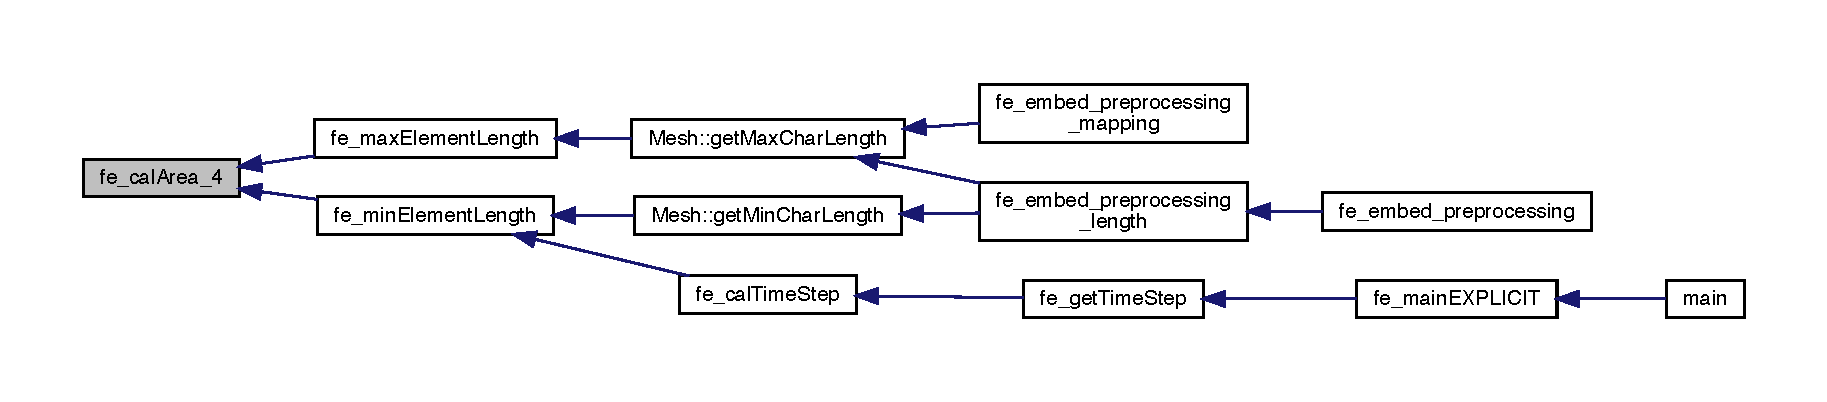
\includegraphics[width=350pt]{functions_8h_ac1306a43db522f3da30471d2a6c48686_icgraph}
\end{center}
\end{figure}
\mbox{\Hypertarget{functions_8h_abbc5cafd6bb8048b69b3bd6f26ceb5f8}\label{functions_8h_abbc5cafd6bb8048b69b3bd6f26ceb5f8}} 
\index{functions.\+h@{functions.\+h}!fe\+\_\+calculate\+\_\+matlmat@{fe\+\_\+calculate\+\_\+matlmat}}
\index{fe\+\_\+calculate\+\_\+matlmat@{fe\+\_\+calculate\+\_\+matlmat}!functions.\+h@{functions.\+h}}
\subsubsection{\texorpdfstring{fe\+\_\+calculate\+\_\+matlmat()}{fe\_calculate\_matlmat()}}
{\footnotesize\ttfamily Matrix\+Xd fe\+\_\+calculate\+\_\+matlmat (\begin{DoxyParamCaption}\item[{int}]{n,  }\item[{double}]{E,  }\item[{double}]{nu }\end{DoxyParamCaption})}

Create material matrix for isotropic elastic case 

Definition at line \hyperlink{fe__simple__elastic_8cpp_source_l00020}{20} of file \hyperlink{fe__simple__elastic_8cpp_source}{fe\+\_\+simple\+\_\+elastic.\+cpp}.

Here is the caller graph for this function\+:\nopagebreak
\begin{figure}[H]
\begin{center}
\leavevmode
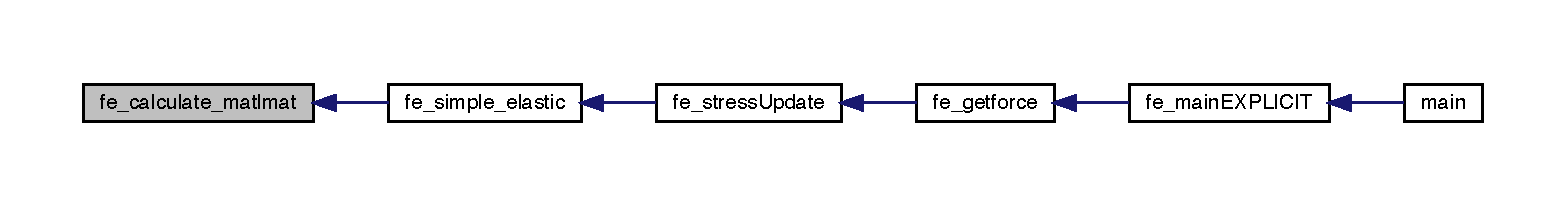
\includegraphics[width=350pt]{functions_8h_abbc5cafd6bb8048b69b3bd6f26ceb5f8_icgraph}
\end{center}
\end{figure}
\mbox{\Hypertarget{functions_8h_a049ed85fefb5b5e80e42432fdcc640fa}\label{functions_8h_a049ed85fefb5b5e80e42432fdcc640fa}} 
\index{functions.\+h@{functions.\+h}!fe\+\_\+calculate\+Accln@{fe\+\_\+calculate\+Accln}}
\index{fe\+\_\+calculate\+Accln@{fe\+\_\+calculate\+Accln}!functions.\+h@{functions.\+h}}
\subsubsection{\texorpdfstring{fe\+\_\+calculate\+Accln()}{fe\_calculateAccln()}}
{\footnotesize\ttfamily Vector\+Xd fe\+\_\+calculate\+Accln (\begin{DoxyParamCaption}\item[{Vector\+Xd}]{mm,  }\item[{Vector\+Xd}]{F\+\_\+net }\end{DoxyParamCaption})}



Definition at line \hyperlink{fe__calculate_accln_8cpp_source_l00005}{5} of file \hyperlink{fe__calculate_accln_8cpp_source}{fe\+\_\+calculate\+Accln.\+cpp}.

Here is the caller graph for this function\+:\nopagebreak
\begin{figure}[H]
\begin{center}
\leavevmode
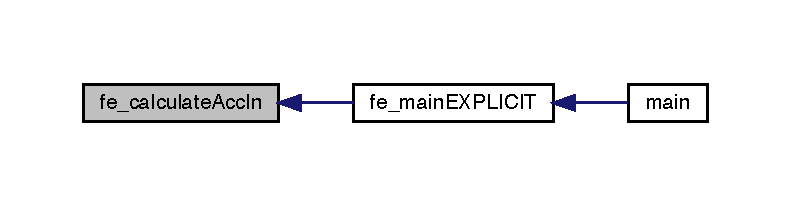
\includegraphics[width=350pt]{functions_8h_a049ed85fefb5b5e80e42432fdcc640fa_icgraph}
\end{center}
\end{figure}
\mbox{\Hypertarget{functions_8h_afb8a8298008daf8f2e705a9acb72b984}\label{functions_8h_afb8a8298008daf8f2e705a9acb72b984}} 
\index{functions.\+h@{functions.\+h}!fe\+\_\+calculate\+KE@{fe\+\_\+calculate\+KE}}
\index{fe\+\_\+calculate\+KE@{fe\+\_\+calculate\+KE}!functions.\+h@{functions.\+h}}
\subsubsection{\texorpdfstring{fe\+\_\+calculate\+K\+E()}{fe\_calculateKE()}\hspace{0.1cm}{\footnotesize\ttfamily [1/2]}}
{\footnotesize\ttfamily double fe\+\_\+calculate\+KE (\begin{DoxyParamCaption}\item[{Vector\+Xd}]{mm,  }\item[{Vector\+Xd}]{V }\end{DoxyParamCaption})}



Definition at line \hyperlink{fe__calculate_k_e_8cpp_source_l00005}{5} of file \hyperlink{fe__calculate_k_e_8cpp_source}{fe\+\_\+calculate\+K\+E.\+cpp}.

Here is the caller graph for this function\+:\nopagebreak
\begin{figure}[H]
\begin{center}
\leavevmode
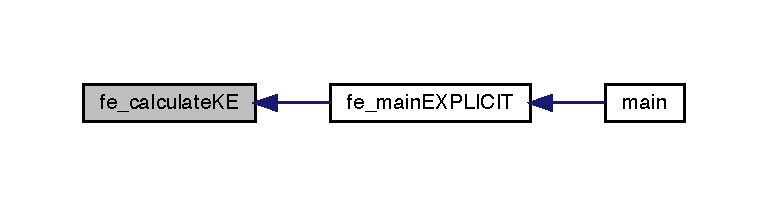
\includegraphics[width=350pt]{functions_8h_afb8a8298008daf8f2e705a9acb72b984_icgraph}
\end{center}
\end{figure}
\mbox{\Hypertarget{functions_8h_a0bdf25bf63fdb63302feaecb1284626e}\label{functions_8h_a0bdf25bf63fdb63302feaecb1284626e}} 
\index{functions.\+h@{functions.\+h}!fe\+\_\+calculate\+KE@{fe\+\_\+calculate\+KE}}
\index{fe\+\_\+calculate\+KE@{fe\+\_\+calculate\+KE}!functions.\+h@{functions.\+h}}
\subsubsection{\texorpdfstring{fe\+\_\+calculate\+K\+E()}{fe\_calculateKE()}\hspace{0.1cm}{\footnotesize\ttfamily [2/2]}}
{\footnotesize\ttfamily double fe\+\_\+calculate\+KE (\begin{DoxyParamCaption}\item[{Matrix\+Xd}]{mm,  }\item[{Vector\+Xd}]{V }\end{DoxyParamCaption})}



Definition at line \hyperlink{fe__calculate_k_e_8cpp_source_l00015}{15} of file \hyperlink{fe__calculate_k_e_8cpp_source}{fe\+\_\+calculate\+K\+E.\+cpp}.

\mbox{\Hypertarget{functions_8h_abeed10bd80ae1f3c95d79c4aed512d8f}\label{functions_8h_abeed10bd80ae1f3c95d79c4aed512d8f}} 
\index{functions.\+h@{functions.\+h}!fe\+\_\+calculate\+Mass@{fe\+\_\+calculate\+Mass}}
\index{fe\+\_\+calculate\+Mass@{fe\+\_\+calculate\+Mass}!functions.\+h@{functions.\+h}}
\subsubsection{\texorpdfstring{fe\+\_\+calculate\+Mass()}{fe\_calculateMass()}}
{\footnotesize\ttfamily Vector\+Xd fe\+\_\+calculate\+Mass (\begin{DoxyParamCaption}\item[{Vector\+Xd}]{mm,  }\item[{std\+::string}]{type }\end{DoxyParamCaption})}



Definition at line \hyperlink{fe__calculate_mass_8cpp_source_l00005}{5} of file \hyperlink{fe__calculate_mass_8cpp_source}{fe\+\_\+calculate\+Mass.\+cpp}.

Here is the call graph for this function\+:\nopagebreak
\begin{figure}[H]
\begin{center}
\leavevmode
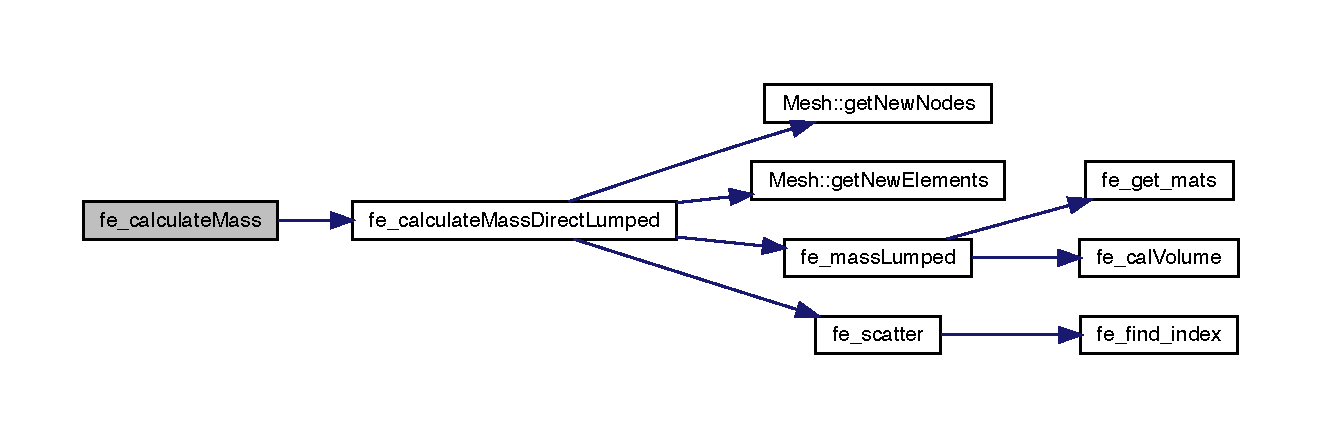
\includegraphics[width=350pt]{functions_8h_abeed10bd80ae1f3c95d79c4aed512d8f_cgraph}
\end{center}
\end{figure}
Here is the caller graph for this function\+:\nopagebreak
\begin{figure}[H]
\begin{center}
\leavevmode
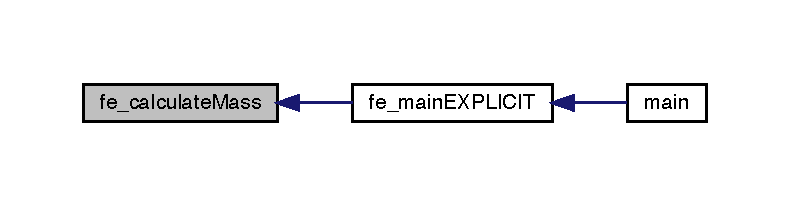
\includegraphics[width=350pt]{functions_8h_abeed10bd80ae1f3c95d79c4aed512d8f_icgraph}
\end{center}
\end{figure}
\mbox{\Hypertarget{functions_8h_aca6d101baf8887cf61064067985cbd62}\label{functions_8h_aca6d101baf8887cf61064067985cbd62}} 
\index{functions.\+h@{functions.\+h}!fe\+\_\+calculate\+Mass\+Direct\+Lumped@{fe\+\_\+calculate\+Mass\+Direct\+Lumped}}
\index{fe\+\_\+calculate\+Mass\+Direct\+Lumped@{fe\+\_\+calculate\+Mass\+Direct\+Lumped}!functions.\+h@{functions.\+h}}
\subsubsection{\texorpdfstring{fe\+\_\+calculate\+Mass\+Direct\+Lumped()}{fe\_calculateMassDirectLumped()}}
{\footnotesize\ttfamily Vector\+Xd fe\+\_\+calculate\+Mass\+Direct\+Lumped (\begin{DoxyParamCaption}\item[{Vector\+Xd}]{mm }\end{DoxyParamCaption})}

number of elements 

Definition at line \hyperlink{fe__calculate_mass_8cpp_source_l00014}{14} of file \hyperlink{fe__calculate_mass_8cpp_source}{fe\+\_\+calculate\+Mass.\+cpp}.

Here is the call graph for this function\+:\nopagebreak
\begin{figure}[H]
\begin{center}
\leavevmode
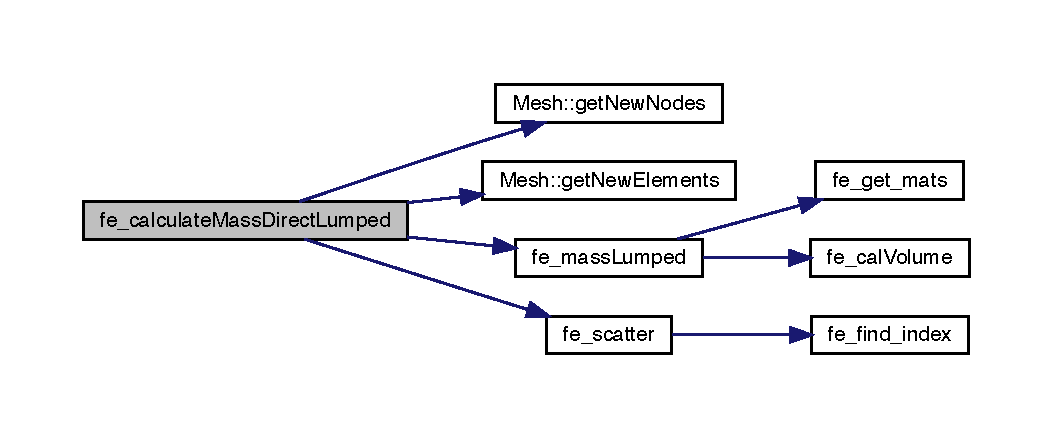
\includegraphics[width=350pt]{functions_8h_aca6d101baf8887cf61064067985cbd62_cgraph}
\end{center}
\end{figure}
Here is the caller graph for this function\+:\nopagebreak
\begin{figure}[H]
\begin{center}
\leavevmode
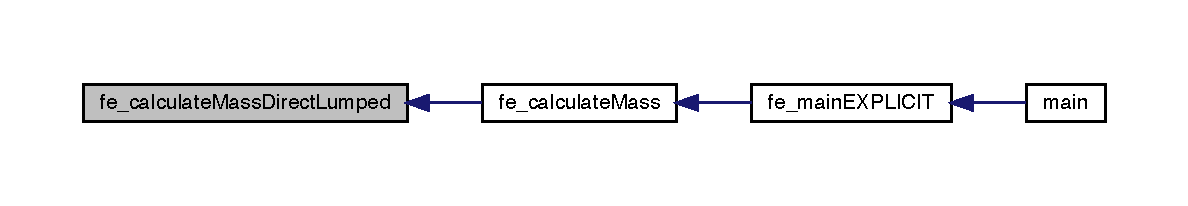
\includegraphics[width=350pt]{functions_8h_aca6d101baf8887cf61064067985cbd62_icgraph}
\end{center}
\end{figure}
\mbox{\Hypertarget{functions_8h_ae50379f74802347e04dbc022897f9cb0}\label{functions_8h_ae50379f74802347e04dbc022897f9cb0}} 
\index{functions.\+h@{functions.\+h}!fe\+\_\+cal\+Def\+Grad@{fe\+\_\+cal\+Def\+Grad}}
\index{fe\+\_\+cal\+Def\+Grad@{fe\+\_\+cal\+Def\+Grad}!functions.\+h@{functions.\+h}}
\subsubsection{\texorpdfstring{fe\+\_\+cal\+Def\+Grad()}{fe\_calDefGrad()}}
{\footnotesize\ttfamily Matrix\+Xd fe\+\_\+cal\+Def\+Grad (\begin{DoxyParamCaption}\item[{Vector\+Xd}]{dndx,  }\item[{Vector\+Xd}]{dndy,  }\item[{Vector\+Xd}]{dndz,  }\item[{Vector\+Xd}]{u }\end{DoxyParamCaption})}

Calculates the deformation gradient 

Definition at line \hyperlink{fe__cal_def_grad_8cpp_source_l00008}{8} of file \hyperlink{fe__cal_def_grad_8cpp_source}{fe\+\_\+cal\+Def\+Grad.\+cpp}.

Here is the caller graph for this function\+:\nopagebreak
\begin{figure}[H]
\begin{center}
\leavevmode
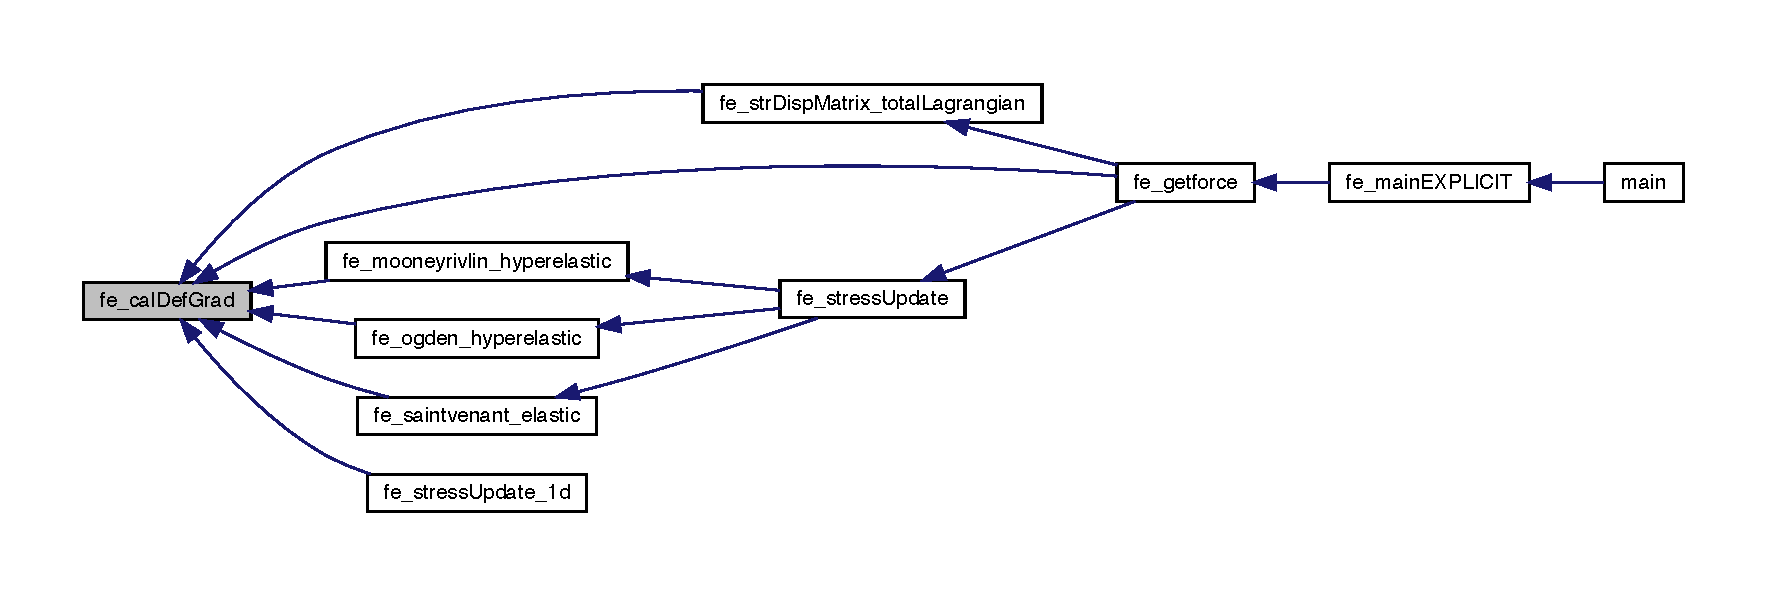
\includegraphics[width=350pt]{functions_8h_ae50379f74802347e04dbc022897f9cb0_icgraph}
\end{center}
\end{figure}
\mbox{\Hypertarget{functions_8h_a5ae3771e65b4a0d177097041a4349c28}\label{functions_8h_a5ae3771e65b4a0d177097041a4349c28}} 
\index{functions.\+h@{functions.\+h}!fe\+\_\+cal\+Jacobian@{fe\+\_\+cal\+Jacobian}}
\index{fe\+\_\+cal\+Jacobian@{fe\+\_\+cal\+Jacobian}!functions.\+h@{functions.\+h}}
\subsubsection{\texorpdfstring{fe\+\_\+cal\+Jacobian()}{fe\_calJacobian()}}
{\footnotesize\ttfamily Matrix\+Xd fe\+\_\+cal\+Jacobian (\begin{DoxyParamCaption}\item[{int}]{dim,  }\item[{int}]{nnel,  }\item[{Vector\+Xd}]{dndr,  }\item[{Vector\+Xd}]{dnds,  }\item[{Vector\+Xd}]{dndt,  }\item[{Vector\+Xd}]{xcoord,  }\item[{Vector\+Xd}]{ycoord,  }\item[{Vector\+Xd}]{zcoord }\end{DoxyParamCaption})}

Calculates the jacobian -- using the derivates of shape functions 

Definition at line \hyperlink{fe__cal_jacobian_8cpp_source_l00007}{7} of file \hyperlink{fe__cal_jacobian_8cpp_source}{fe\+\_\+cal\+Jacobian.\+cpp}.

Here is the caller graph for this function\+:\nopagebreak
\begin{figure}[H]
\begin{center}
\leavevmode
\includegraphics[width=350pt]{functions_8h_a5ae3771e65b4a0d177097041a4349c28_icgraph}
\end{center}
\end{figure}
\mbox{\Hypertarget{functions_8h_ae2eeba997bf4f0bc4749b92130de7ba3}\label{functions_8h_ae2eeba997bf4f0bc4749b92130de7ba3}} 
\index{functions.\+h@{functions.\+h}!fe\+\_\+cal\+Simp\+Transformation@{fe\+\_\+cal\+Simp\+Transformation}}
\index{fe\+\_\+cal\+Simp\+Transformation@{fe\+\_\+cal\+Simp\+Transformation}!functions.\+h@{functions.\+h}}
\subsubsection{\texorpdfstring{fe\+\_\+cal\+Simp\+Transformation()}{fe\_calSimpTransformation()}}
{\footnotesize\ttfamily Matrix\+Xd fe\+\_\+cal\+Simp\+Transformation (\begin{DoxyParamCaption}\item[{Matrix\+Xd}]{truss\+\_\+nodes }\end{DoxyParamCaption})}



Definition at line \hyperlink{fe__cal_simp_transformation_8cpp_source_l00007}{7} of file \hyperlink{fe__cal_simp_transformation_8cpp_source}{fe\+\_\+cal\+Simp\+Transformation.\+cpp}.

Here is the caller graph for this function\+:\nopagebreak
\begin{figure}[H]
\begin{center}
\leavevmode
\includegraphics[width=350pt]{functions_8h_ae2eeba997bf4f0bc4749b92130de7ba3_icgraph}
\end{center}
\end{figure}
\mbox{\Hypertarget{functions_8h_a295b08cc71d5af080f0450614a01a4e6}\label{functions_8h_a295b08cc71d5af080f0450614a01a4e6}} 
\index{functions.\+h@{functions.\+h}!fe\+\_\+cal\+Time\+Step@{fe\+\_\+cal\+Time\+Step}}
\index{fe\+\_\+cal\+Time\+Step@{fe\+\_\+cal\+Time\+Step}!functions.\+h@{functions.\+h}}
\subsubsection{\texorpdfstring{fe\+\_\+cal\+Time\+Step()}{fe\_calTimeStep()}}
{\footnotesize\ttfamily double fe\+\_\+cal\+Time\+Step (\begin{DoxyParamCaption}\item[{Vector\+Xd}]{xcoord,  }\item[{Vector\+Xd}]{ycoord,  }\item[{Vector\+Xd}]{zcoord,  }\item[{int}]{material\+\_\+id }\end{DoxyParamCaption})}

Calculates the time step for a single element based on its dimensions and material model

For a single element -\/ this function calculates the volume of the element and calculates the critical time step based on the wave speed. 

Definition at line \hyperlink{fe__cal_time_step_8cpp_source_l00005}{5} of file \hyperlink{fe__cal_time_step_8cpp_source}{fe\+\_\+cal\+Time\+Step.\+cpp}.

Here is the call graph for this function\+:\nopagebreak
\begin{figure}[H]
\begin{center}
\leavevmode
\includegraphics[width=350pt]{functions_8h_a295b08cc71d5af080f0450614a01a4e6_cgraph}
\end{center}
\end{figure}
Here is the caller graph for this function\+:\nopagebreak
\begin{figure}[H]
\begin{center}
\leavevmode
\includegraphics[width=350pt]{functions_8h_a295b08cc71d5af080f0450614a01a4e6_icgraph}
\end{center}
\end{figure}
\mbox{\Hypertarget{functions_8h_aa41c40dffea4251a07a8a3f5062f47ae}\label{functions_8h_aa41c40dffea4251a07a8a3f5062f47ae}} 
\index{functions.\+h@{functions.\+h}!fe\+\_\+cal\+Transformation@{fe\+\_\+cal\+Transformation}}
\index{fe\+\_\+cal\+Transformation@{fe\+\_\+cal\+Transformation}!functions.\+h@{functions.\+h}}
\subsubsection{\texorpdfstring{fe\+\_\+cal\+Transformation()}{fe\_calTransformation()}}
{\footnotesize\ttfamily Matrix\+Xd fe\+\_\+cal\+Transformation (\begin{DoxyParamCaption}\item[{Matrix\+Xd}]{truss\+\_\+nodes,  }\item[{int}]{choice }\end{DoxyParamCaption})}

Calculates the transformation matrix -\/ transformation from local (truss) coordinate system to global (3d hex) coordinate system 

Definition at line \hyperlink{fe__cal_transformation_8cpp_source_l00007}{7} of file \hyperlink{fe__cal_transformation_8cpp_source}{fe\+\_\+cal\+Transformation.\+cpp}.

Here is the caller graph for this function\+:\nopagebreak
\begin{figure}[H]
\begin{center}
\leavevmode
\includegraphics[width=331pt]{functions_8h_aa41c40dffea4251a07a8a3f5062f47ae_icgraph}
\end{center}
\end{figure}
\mbox{\Hypertarget{functions_8h_a00f586c9a4bc56ec486776402fc26605}\label{functions_8h_a00f586c9a4bc56ec486776402fc26605}} 
\index{functions.\+h@{functions.\+h}!fe\+\_\+cal\+Volume@{fe\+\_\+cal\+Volume}}
\index{fe\+\_\+cal\+Volume@{fe\+\_\+cal\+Volume}!functions.\+h@{functions.\+h}}
\subsubsection{\texorpdfstring{fe\+\_\+cal\+Volume()}{fe\_calVolume()}}
{\footnotesize\ttfamily double fe\+\_\+cal\+Volume (\begin{DoxyParamCaption}\item[{Vector\+Xd}]{xcoord,  }\item[{Vector\+Xd}]{ycoord,  }\item[{Vector\+Xd}]{zcoord }\end{DoxyParamCaption})}

Calculates the volume of a 3d element 

Definition at line \hyperlink{fe__cal_volume_8cpp_source_l00006}{6} of file \hyperlink{fe__cal_volume_8cpp_source}{fe\+\_\+cal\+Volume.\+cpp}.

Here is the caller graph for this function\+:\nopagebreak
\begin{figure}[H]
\begin{center}
\leavevmode
\includegraphics[width=350pt]{functions_8h_a00f586c9a4bc56ec486776402fc26605_icgraph}
\end{center}
\end{figure}
\mbox{\Hypertarget{functions_8h_a20aed1a2d3d8b470592491a96e60be87}\label{functions_8h_a20aed1a2d3d8b470592491a96e60be87}} 
\index{functions.\+h@{functions.\+h}!fe\+\_\+cal\+Wave\+Speed@{fe\+\_\+cal\+Wave\+Speed}}
\index{fe\+\_\+cal\+Wave\+Speed@{fe\+\_\+cal\+Wave\+Speed}!functions.\+h@{functions.\+h}}
\subsubsection{\texorpdfstring{fe\+\_\+cal\+Wave\+Speed()}{fe\_calWaveSpeed()}}
{\footnotesize\ttfamily double fe\+\_\+cal\+Wave\+Speed (\begin{DoxyParamCaption}\item[{int}]{material\+\_\+id }\end{DoxyParamCaption})}

Calculates the wavespeed for a particular material model

This function calculates the wave speed for an element based on its material properties 

Definition at line \hyperlink{fe__cal_wave_speed_8cpp_source_l00006}{6} of file \hyperlink{fe__cal_wave_speed_8cpp_source}{fe\+\_\+cal\+Wave\+Speed.\+cpp}.

Here is the call graph for this function\+:\nopagebreak
\begin{figure}[H]
\begin{center}
\leavevmode
\includegraphics[width=289pt]{functions_8h_a20aed1a2d3d8b470592491a96e60be87_cgraph}
\end{center}
\end{figure}
Here is the caller graph for this function\+:\nopagebreak
\begin{figure}[H]
\begin{center}
\leavevmode
\includegraphics[width=350pt]{functions_8h_a20aed1a2d3d8b470592491a96e60be87_icgraph}
\end{center}
\end{figure}
\mbox{\Hypertarget{functions_8h_a453ba6bc1e7d5a63db9d56beb6077a27}\label{functions_8h_a453ba6bc1e7d5a63db9d56beb6077a27}} 
\index{functions.\+h@{functions.\+h}!fe\+\_\+compute\+\_\+host@{fe\+\_\+compute\+\_\+host}}
\index{fe\+\_\+compute\+\_\+host@{fe\+\_\+compute\+\_\+host}!functions.\+h@{functions.\+h}}
\subsubsection{\texorpdfstring{fe\+\_\+compute\+\_\+host()}{fe\_compute\_host()}}
{\footnotesize\ttfamily int fe\+\_\+compute\+\_\+host (\begin{DoxyParamCaption}\item[{Vector\+Xd}]{A,  }\item[{Matrix\+Xd}]{nodes\+\_\+host,  }\item[{Matrix\+Xd}]{elements\+\_\+host\+\_\+tmp }\end{DoxyParamCaption})}



Definition at line \hyperlink{fe__compute__host_8cpp_source_l00004}{4} of file \hyperlink{fe__compute__host_8cpp_source}{fe\+\_\+compute\+\_\+host.\+cpp}.

Here is the call graph for this function\+:\nopagebreak
\begin{figure}[H]
\begin{center}
\leavevmode
\includegraphics[width=255pt]{functions_8h_a453ba6bc1e7d5a63db9d56beb6077a27_cgraph}
\end{center}
\end{figure}
Here is the caller graph for this function\+:\nopagebreak
\begin{figure}[H]
\begin{center}
\leavevmode
\includegraphics[width=338pt]{functions_8h_a453ba6bc1e7d5a63db9d56beb6077a27_icgraph}
\end{center}
\end{figure}
\mbox{\Hypertarget{functions_8h_ac2d90cb6719488bc8551e6f9437f4f76}\label{functions_8h_ac2d90cb6719488bc8551e6f9437f4f76}} 
\index{functions.\+h@{functions.\+h}!fe\+\_\+concatenate\+\_\+vector2matrix@{fe\+\_\+concatenate\+\_\+vector2matrix}}
\index{fe\+\_\+concatenate\+\_\+vector2matrix@{fe\+\_\+concatenate\+\_\+vector2matrix}!functions.\+h@{functions.\+h}}
\subsubsection{\texorpdfstring{fe\+\_\+concatenate\+\_\+vector2matrix()}{fe\_concatenate\_vector2matrix()}}
{\footnotesize\ttfamily Matrix\+Xd fe\+\_\+concatenate\+\_\+vector2matrix (\begin{DoxyParamCaption}\item[{Matrix\+Xd}]{A,  }\item[{Vector\+Xd}]{B,  }\item[{int}]{opt }\end{DoxyParamCaption})}

Concatenate a vector to a matrix -- rowwise or coloumn wise 

Definition at line \hyperlink{fe__concatenate__vector2matrix_8cpp_source_l00005}{5} of file \hyperlink{fe__concatenate__vector2matrix_8cpp_source}{fe\+\_\+concatenate\+\_\+vector2matrix.\+cpp}.

Here is the caller graph for this function\+:\nopagebreak
\begin{figure}[H]
\begin{center}
\leavevmode
\includegraphics[width=350pt]{functions_8h_ac2d90cb6719488bc8551e6f9437f4f76_icgraph}
\end{center}
\end{figure}
\mbox{\Hypertarget{functions_8h_a150d77644eb280d58564e3ff4885e73c}\label{functions_8h_a150d77644eb280d58564e3ff4885e73c}} 
\index{functions.\+h@{functions.\+h}!fe\+\_\+create\+\_\+bbox@{fe\+\_\+create\+\_\+bbox}}
\index{fe\+\_\+create\+\_\+bbox@{fe\+\_\+create\+\_\+bbox}!functions.\+h@{functions.\+h}}
\subsubsection{\texorpdfstring{fe\+\_\+create\+\_\+bbox()}{fe\_create\_bbox()}}
{\footnotesize\ttfamily Matrix\+Xd fe\+\_\+create\+\_\+bbox (\begin{DoxyParamCaption}\item[{Vector\+Xd}]{A,  }\item[{Matrix\+Xd}]{nodes\+\_\+host,  }\item[{Matrix\+Xd}]{elements\+\_\+host,  }\item[{double}]{length }\end{DoxyParamCaption})}



Definition at line \hyperlink{fe__create__bbox_8cpp_source_l00004}{4} of file \hyperlink{fe__create__bbox_8cpp_source}{fe\+\_\+create\+\_\+bbox.\+cpp}.

Here is the call graph for this function\+:\nopagebreak
\begin{figure}[H]
\begin{center}
\leavevmode
\includegraphics[width=350pt]{functions_8h_a150d77644eb280d58564e3ff4885e73c_cgraph}
\end{center}
\end{figure}
Here is the caller graph for this function\+:\nopagebreak
\begin{figure}[H]
\begin{center}
\leavevmode
\includegraphics[width=330pt]{functions_8h_a150d77644eb280d58564e3ff4885e73c_icgraph}
\end{center}
\end{figure}
\mbox{\Hypertarget{functions_8h_a5110a192d089c6b26744b9e9d67a7c2d}\label{functions_8h_a5110a192d089c6b26744b9e9d67a7c2d}} 
\index{functions.\+h@{functions.\+h}!fe\+\_\+display\+\_\+matrix@{fe\+\_\+display\+\_\+matrix}}
\index{fe\+\_\+display\+\_\+matrix@{fe\+\_\+display\+\_\+matrix}!functions.\+h@{functions.\+h}}
\subsubsection{\texorpdfstring{fe\+\_\+display\+\_\+matrix()}{fe\_display\_matrix()}}
{\footnotesize\ttfamily void fe\+\_\+display\+\_\+matrix (\begin{DoxyParamCaption}\item[{Matrix\+Xd}]{A }\end{DoxyParamCaption})}

Prints out a matrix 

Definition at line \hyperlink{fe__display_8cpp_source_l00005}{5} of file \hyperlink{fe__display_8cpp_source}{fe\+\_\+display.\+cpp}.

\mbox{\Hypertarget{functions_8h_ab3e39c6d01b6fd10c9e264731cef75dc}\label{functions_8h_ab3e39c6d01b6fd10c9e264731cef75dc}} 
\index{functions.\+h@{functions.\+h}!fe\+\_\+display\+\_\+vector@{fe\+\_\+display\+\_\+vector}}
\index{fe\+\_\+display\+\_\+vector@{fe\+\_\+display\+\_\+vector}!functions.\+h@{functions.\+h}}
\subsubsection{\texorpdfstring{fe\+\_\+display\+\_\+vector()}{fe\_display\_vector()}}
{\footnotesize\ttfamily void fe\+\_\+display\+\_\+vector (\begin{DoxyParamCaption}\item[{Vector\+Xd}]{A }\end{DoxyParamCaption})}

Prints out a vector 

Definition at line \hyperlink{fe__display_8cpp_source_l00041}{41} of file \hyperlink{fe__display_8cpp_source}{fe\+\_\+display.\+cpp}.

\mbox{\Hypertarget{functions_8h_afc547bef246c057db6cbd04bf7f866a9}\label{functions_8h_afc547bef246c057db6cbd04bf7f866a9}} 
\index{functions.\+h@{functions.\+h}!fe\+\_\+dndr\+\_\+8@{fe\+\_\+dndr\+\_\+8}}
\index{fe\+\_\+dndr\+\_\+8@{fe\+\_\+dndr\+\_\+8}!functions.\+h@{functions.\+h}}
\subsubsection{\texorpdfstring{fe\+\_\+dndr\+\_\+8()}{fe\_dndr\_8()}}
{\footnotesize\ttfamily Vector\+Xd fe\+\_\+dndr\+\_\+8 (\begin{DoxyParamCaption}\item[{double}]{rvalue,  }\item[{double}]{svalue,  }\item[{double}]{tvalue }\end{DoxyParamCaption})}

dndr of isoparametric element calculated for particular r, s, and t 

Definition at line \hyperlink{fe__dn__iso__8_8cpp_source_l00006}{6} of file \hyperlink{fe__dn__iso__8_8cpp_source}{fe\+\_\+dn\+\_\+iso\+\_\+8.\+cpp}.

Here is the caller graph for this function\+:\nopagebreak
\begin{figure}[H]
\begin{center}
\leavevmode
\includegraphics[width=350pt]{functions_8h_afc547bef246c057db6cbd04bf7f866a9_icgraph}
\end{center}
\end{figure}
\mbox{\Hypertarget{functions_8h_ac0b5524525e1f2e89bb064c15ab8e664}\label{functions_8h_ac0b5524525e1f2e89bb064c15ab8e664}} 
\index{functions.\+h@{functions.\+h}!fe\+\_\+dnds\+\_\+8@{fe\+\_\+dnds\+\_\+8}}
\index{fe\+\_\+dnds\+\_\+8@{fe\+\_\+dnds\+\_\+8}!functions.\+h@{functions.\+h}}
\subsubsection{\texorpdfstring{fe\+\_\+dnds\+\_\+8()}{fe\_dnds\_8()}}
{\footnotesize\ttfamily Vector\+Xd fe\+\_\+dnds\+\_\+8 (\begin{DoxyParamCaption}\item[{double}]{rvalue,  }\item[{double}]{svalue,  }\item[{double}]{tvalue }\end{DoxyParamCaption})}

dnds of isoparametric element calculated for particular r, s, and t 

Definition at line \hyperlink{fe__dn__iso__8_8cpp_source_l00044}{44} of file \hyperlink{fe__dn__iso__8_8cpp_source}{fe\+\_\+dn\+\_\+iso\+\_\+8.\+cpp}.

Here is the caller graph for this function\+:\nopagebreak
\begin{figure}[H]
\begin{center}
\leavevmode
\includegraphics[width=350pt]{functions_8h_ac0b5524525e1f2e89bb064c15ab8e664_icgraph}
\end{center}
\end{figure}
\mbox{\Hypertarget{functions_8h_a57e8e5c9f740c98e4767f29c121c2d0a}\label{functions_8h_a57e8e5c9f740c98e4767f29c121c2d0a}} 
\index{functions.\+h@{functions.\+h}!fe\+\_\+dndt\+\_\+8@{fe\+\_\+dndt\+\_\+8}}
\index{fe\+\_\+dndt\+\_\+8@{fe\+\_\+dndt\+\_\+8}!functions.\+h@{functions.\+h}}
\subsubsection{\texorpdfstring{fe\+\_\+dndt\+\_\+8()}{fe\_dndt\_8()}}
{\footnotesize\ttfamily Vector\+Xd fe\+\_\+dndt\+\_\+8 (\begin{DoxyParamCaption}\item[{double}]{rvalue,  }\item[{double}]{svalue,  }\item[{double}]{tvalue }\end{DoxyParamCaption})}

dndt of isoparametric element calculated for particular r, s, and t 

Definition at line \hyperlink{fe__dn__iso__8_8cpp_source_l00082}{82} of file \hyperlink{fe__dn__iso__8_8cpp_source}{fe\+\_\+dn\+\_\+iso\+\_\+8.\+cpp}.

Here is the caller graph for this function\+:\nopagebreak
\begin{figure}[H]
\begin{center}
\leavevmode
\includegraphics[width=350pt]{functions_8h_a57e8e5c9f740c98e4767f29c121c2d0a_icgraph}
\end{center}
\end{figure}
\mbox{\Hypertarget{functions_8h_afc6be1a5667e68156cb099e8da71170f}\label{functions_8h_afc6be1a5667e68156cb099e8da71170f}} 
\index{functions.\+h@{functions.\+h}!fe\+\_\+dndx\+\_\+8@{fe\+\_\+dndx\+\_\+8}}
\index{fe\+\_\+dndx\+\_\+8@{fe\+\_\+dndx\+\_\+8}!functions.\+h@{functions.\+h}}
\subsubsection{\texorpdfstring{fe\+\_\+dndx\+\_\+8()}{fe\_dndx\_8()}}
{\footnotesize\ttfamily Vector\+Xd fe\+\_\+dndx\+\_\+8 (\begin{DoxyParamCaption}\item[{int}]{nnel,  }\item[{Vector\+Xd}]{dndr,  }\item[{Vector\+Xd}]{dnds,  }\item[{Vector\+Xd}]{dndt,  }\item[{Matrix\+Xd}]{inv\+Jacobian }\end{DoxyParamCaption})}

dndx of actual element calculates using jacobian and shape function derivates calculated in the isoparametric element 

Definition at line \hyperlink{fe__dn__actual__8_8cpp_source_l00006}{6} of file \hyperlink{fe__dn__actual__8_8cpp_source}{fe\+\_\+dn\+\_\+actual\+\_\+8.\+cpp}.

Here is the caller graph for this function\+:\nopagebreak
\begin{figure}[H]
\begin{center}
\leavevmode
\includegraphics[width=350pt]{functions_8h_afc6be1a5667e68156cb099e8da71170f_icgraph}
\end{center}
\end{figure}
\mbox{\Hypertarget{functions_8h_a0572d7818e085c67f7fbb84eef8ecfb4}\label{functions_8h_a0572d7818e085c67f7fbb84eef8ecfb4}} 
\index{functions.\+h@{functions.\+h}!fe\+\_\+dndy\+\_\+8@{fe\+\_\+dndy\+\_\+8}}
\index{fe\+\_\+dndy\+\_\+8@{fe\+\_\+dndy\+\_\+8}!functions.\+h@{functions.\+h}}
\subsubsection{\texorpdfstring{fe\+\_\+dndy\+\_\+8()}{fe\_dndy\_8()}}
{\footnotesize\ttfamily Vector\+Xd fe\+\_\+dndy\+\_\+8 (\begin{DoxyParamCaption}\item[{int}]{nnel,  }\item[{Vector\+Xd}]{dndr,  }\item[{Vector\+Xd}]{dnds,  }\item[{Vector\+Xd}]{dndt,  }\item[{Matrix\+Xd}]{inv\+Jacobian }\end{DoxyParamCaption})}

dndy of actual element calculates using jacobian and shape function derivates calculated in the isoparametric element 

Definition at line \hyperlink{fe__dn__actual__8_8cpp_source_l00017}{17} of file \hyperlink{fe__dn__actual__8_8cpp_source}{fe\+\_\+dn\+\_\+actual\+\_\+8.\+cpp}.

Here is the caller graph for this function\+:\nopagebreak
\begin{figure}[H]
\begin{center}
\leavevmode
\includegraphics[width=350pt]{functions_8h_a0572d7818e085c67f7fbb84eef8ecfb4_icgraph}
\end{center}
\end{figure}
\mbox{\Hypertarget{functions_8h_aaf75db8433433807839c6ea17f2cf72c}\label{functions_8h_aaf75db8433433807839c6ea17f2cf72c}} 
\index{functions.\+h@{functions.\+h}!fe\+\_\+dndz\+\_\+8@{fe\+\_\+dndz\+\_\+8}}
\index{fe\+\_\+dndz\+\_\+8@{fe\+\_\+dndz\+\_\+8}!functions.\+h@{functions.\+h}}
\subsubsection{\texorpdfstring{fe\+\_\+dndz\+\_\+8()}{fe\_dndz\_8()}}
{\footnotesize\ttfamily Vector\+Xd fe\+\_\+dndz\+\_\+8 (\begin{DoxyParamCaption}\item[{int}]{nnel,  }\item[{Vector\+Xd}]{dndr,  }\item[{Vector\+Xd}]{dnds,  }\item[{Vector\+Xd}]{dndt,  }\item[{Matrix\+Xd}]{inv\+Jacobian }\end{DoxyParamCaption})}

dndz of actual element calculates using jacobian and shape function derivates calculated in the isoparametric element 

Definition at line \hyperlink{fe__dn__actual__8_8cpp_source_l00028}{28} of file \hyperlink{fe__dn__actual__8_8cpp_source}{fe\+\_\+dn\+\_\+actual\+\_\+8.\+cpp}.

Here is the caller graph for this function\+:\nopagebreak
\begin{figure}[H]
\begin{center}
\leavevmode
\includegraphics[width=350pt]{functions_8h_aaf75db8433433807839c6ea17f2cf72c_icgraph}
\end{center}
\end{figure}
\mbox{\Hypertarget{functions_8h_a840ddc7df1916f6b5dfbb141adac32d3}\label{functions_8h_a840ddc7df1916f6b5dfbb141adac32d3}} 
\index{functions.\+h@{functions.\+h}!fe\+\_\+embed\+\_\+preprocessing@{fe\+\_\+embed\+\_\+preprocessing}}
\index{fe\+\_\+embed\+\_\+preprocessing@{fe\+\_\+embed\+\_\+preprocessing}!functions.\+h@{functions.\+h}}
\subsubsection{\texorpdfstring{fe\+\_\+embed\+\_\+preprocessing()}{fe\_embed\_preprocessing()}}
{\footnotesize\ttfamily Vector\+Xd fe\+\_\+embed\+\_\+preprocessing (\begin{DoxyParamCaption}\item[{\hyperlink{class_mesh}{Mesh}}]{host,  }\item[{\hyperlink{class_mesh}{Mesh}}]{embed }\end{DoxyParamCaption})}

This function carries out all the required pre-\/processing steps for embedded element constraint 

Definition at line \hyperlink{fe__embed__preprocessing_8cpp_source_l00007}{7} of file \hyperlink{fe__embed__preprocessing_8cpp_source}{fe\+\_\+embed\+\_\+preprocessing.\+cpp}.

Here is the call graph for this function\+:\nopagebreak
\begin{figure}[H]
\begin{center}
\leavevmode
\includegraphics[width=350pt]{functions_8h_a840ddc7df1916f6b5dfbb141adac32d3_cgraph}
\end{center}
\end{figure}
\mbox{\Hypertarget{functions_8h_a50e8d7839525058d40e3a53f9d5de77c}\label{functions_8h_a50e8d7839525058d40e3a53f9d5de77c}} 
\index{functions.\+h@{functions.\+h}!fe\+\_\+embed\+\_\+preprocessing\+\_\+length@{fe\+\_\+embed\+\_\+preprocessing\+\_\+length}}
\index{fe\+\_\+embed\+\_\+preprocessing\+\_\+length@{fe\+\_\+embed\+\_\+preprocessing\+\_\+length}!functions.\+h@{functions.\+h}}
\subsubsection{\texorpdfstring{fe\+\_\+embed\+\_\+preprocessing\+\_\+length()}{fe\_embed\_preprocessing\_length()}}
{\footnotesize\ttfamily void fe\+\_\+embed\+\_\+preprocessing\+\_\+length (\begin{DoxyParamCaption}\item[{\hyperlink{class_mesh}{Mesh}}]{host,  }\item[{\hyperlink{class_mesh}{Mesh}}]{embed }\end{DoxyParamCaption})}

Checks if the host mesh has zero length edges

Checks if the embedded mesh has zero length edges 

Definition at line \hyperlink{fe__embed__preprocessing_8cpp_source_l00013}{13} of file \hyperlink{fe__embed__preprocessing_8cpp_source}{fe\+\_\+embed\+\_\+preprocessing.\+cpp}.

Here is the call graph for this function\+:\nopagebreak
\begin{figure}[H]
\begin{center}
\leavevmode
\includegraphics[width=350pt]{functions_8h_a50e8d7839525058d40e3a53f9d5de77c_cgraph}
\end{center}
\end{figure}
Here is the caller graph for this function\+:\nopagebreak
\begin{figure}[H]
\begin{center}
\leavevmode
\includegraphics[width=350pt]{functions_8h_a50e8d7839525058d40e3a53f9d5de77c_icgraph}
\end{center}
\end{figure}
\mbox{\Hypertarget{functions_8h_a0600721e5cf84d84408ce9605b004610}\label{functions_8h_a0600721e5cf84d84408ce9605b004610}} 
\index{functions.\+h@{functions.\+h}!fe\+\_\+embed\+\_\+preprocessing\+\_\+mapping@{fe\+\_\+embed\+\_\+preprocessing\+\_\+mapping}}
\index{fe\+\_\+embed\+\_\+preprocessing\+\_\+mapping@{fe\+\_\+embed\+\_\+preprocessing\+\_\+mapping}!functions.\+h@{functions.\+h}}
\subsubsection{\texorpdfstring{fe\+\_\+embed\+\_\+preprocessing\+\_\+mapping()}{fe\_embed\_preprocessing\_mapping()}}
{\footnotesize\ttfamily Vector\+Xd fe\+\_\+embed\+\_\+preprocessing\+\_\+mapping (\begin{DoxyParamCaption}\item[{\hyperlink{class_mesh}{Mesh}}]{host,  }\item[{\hyperlink{class_mesh}{Mesh}}]{embed }\end{DoxyParamCaption})}

Temporary Matrices useful in the mapping scheme

Creates a bounding box and seperates the mesh in the bouding box from the whole mesh 

Definition at line \hyperlink{fe__embed__preprocessing__mapping_8cpp_source_l00004}{4} of file \hyperlink{fe__embed__preprocessing__mapping_8cpp_source}{fe\+\_\+embed\+\_\+preprocessing\+\_\+mapping.\+cpp}.

Here is the call graph for this function\+:\nopagebreak
\begin{figure}[H]
\begin{center}
\leavevmode
\includegraphics[width=350pt]{functions_8h_a0600721e5cf84d84408ce9605b004610_cgraph}
\end{center}
\end{figure}
\mbox{\Hypertarget{functions_8h_a983304137f9a961469a558437d5d2d59}\label{functions_8h_a983304137f9a961469a558437d5d2d59}} 
\index{functions.\+h@{functions.\+h}!fe\+\_\+find@{fe\+\_\+find}}
\index{fe\+\_\+find@{fe\+\_\+find}!functions.\+h@{functions.\+h}}
\subsubsection{\texorpdfstring{fe\+\_\+find()}{fe\_find()}\hspace{0.1cm}{\footnotesize\ttfamily [1/2]}}
{\footnotesize\ttfamily int fe\+\_\+find (\begin{DoxyParamCaption}\item[{Vector\+Xd}]{A,  }\item[{double}]{a }\end{DoxyParamCaption})}

find the poistion index of a double value in a vector -- analogous to \textquotesingle{}find\textquotesingle{} function in M\+A\+T\+L\+AB 

Definition at line \hyperlink{fe__find_8cpp_source_l00004}{4} of file \hyperlink{fe__find_8cpp_source}{fe\+\_\+find.\+cpp}.

Here is the caller graph for this function\+:\nopagebreak
\begin{figure}[H]
\begin{center}
\leavevmode
\includegraphics[width=350pt]{functions_8h_a983304137f9a961469a558437d5d2d59_icgraph}
\end{center}
\end{figure}
\mbox{\Hypertarget{functions_8h_a0d42c56d98efb23079057340a7133e89}\label{functions_8h_a0d42c56d98efb23079057340a7133e89}} 
\index{functions.\+h@{functions.\+h}!fe\+\_\+find@{fe\+\_\+find}}
\index{fe\+\_\+find@{fe\+\_\+find}!functions.\+h@{functions.\+h}}
\subsubsection{\texorpdfstring{fe\+\_\+find()}{fe\_find()}\hspace{0.1cm}{\footnotesize\ttfamily [2/2]}}
{\footnotesize\ttfamily int fe\+\_\+find (\begin{DoxyParamCaption}\item[{Vector\+Xd}]{A,  }\item[{int}]{a }\end{DoxyParamCaption})}

find the poistion index of a integer value in a vector -- analogous to \textquotesingle{}find\textquotesingle{} function in M\+A\+T\+L\+AB 

Definition at line \hyperlink{fe__find_8cpp_source_l00018}{18} of file \hyperlink{fe__find_8cpp_source}{fe\+\_\+find.\+cpp}.

\mbox{\Hypertarget{functions_8h_ae4dbe24b761cafa3577afab76726b382}\label{functions_8h_ae4dbe24b761cafa3577afab76726b382}} 
\index{functions.\+h@{functions.\+h}!fe\+\_\+find\+\_\+index@{fe\+\_\+find\+\_\+index}}
\index{fe\+\_\+find\+\_\+index@{fe\+\_\+find\+\_\+index}!functions.\+h@{functions.\+h}}
\subsubsection{\texorpdfstring{fe\+\_\+find\+\_\+index()}{fe\_find\_index()}}
{\footnotesize\ttfamily Vector\+Xi fe\+\_\+find\+\_\+index (\begin{DoxyParamCaption}\item[{Vector\+Xi}]{node\+\_\+list }\end{DoxyParamCaption})}

Find the index based on the D\+OF of a particular node 

Definition at line \hyperlink{fe__find__index_8cpp_source_l00016}{16} of file \hyperlink{fe__find__index_8cpp_source}{fe\+\_\+find\+\_\+index.\+cpp}.

Here is the caller graph for this function\+:\nopagebreak
\begin{figure}[H]
\begin{center}
\leavevmode
\includegraphics[width=350pt]{functions_8h_ae4dbe24b761cafa3577afab76726b382_icgraph}
\end{center}
\end{figure}
\mbox{\Hypertarget{functions_8h_a5ce8a3cf9dcc8b599ac40f7f3a48f196}\label{functions_8h_a5ce8a3cf9dcc8b599ac40f7f3a48f196}} 
\index{functions.\+h@{functions.\+h}!fe\+\_\+function@{fe\+\_\+function}}
\index{fe\+\_\+function@{fe\+\_\+function}!functions.\+h@{functions.\+h}}
\subsubsection{\texorpdfstring{fe\+\_\+function()}{fe\_function()}}
{\footnotesize\ttfamily double fe\+\_\+function (\begin{DoxyParamCaption}\item[{double}]{a,  }\item[{std\+::string}]{b,  }\item[{double}]{time }\end{DoxyParamCaption})}

Function outputs the standard curve values 

Definition at line \hyperlink{fe__function_8cpp_source_l00005}{5} of file \hyperlink{fe__function_8cpp_source}{fe\+\_\+function.\+cpp}.

Here is the caller graph for this function\+:\nopagebreak
\begin{figure}[H]
\begin{center}
\leavevmode
\includegraphics[width=350pt]{functions_8h_a5ce8a3cf9dcc8b599ac40f7f3a48f196_icgraph}
\end{center}
\end{figure}
\mbox{\Hypertarget{functions_8h_afb02d53011656285452b16427dcd08dd}\label{functions_8h_afb02d53011656285452b16427dcd08dd}} 
\index{functions.\+h@{functions.\+h}!fe\+\_\+function\+\_\+d\+\_\+derivative@{fe\+\_\+function\+\_\+d\+\_\+derivative}}
\index{fe\+\_\+function\+\_\+d\+\_\+derivative@{fe\+\_\+function\+\_\+d\+\_\+derivative}!functions.\+h@{functions.\+h}}
\subsubsection{\texorpdfstring{fe\+\_\+function\+\_\+d\+\_\+derivative()}{fe\_function\_d\_derivative()}}
{\footnotesize\ttfamily double fe\+\_\+function\+\_\+d\+\_\+derivative (\begin{DoxyParamCaption}\item[{double}]{a,  }\item[{std\+::string}]{b,  }\item[{double}]{time }\end{DoxyParamCaption})}

Function outputs the double derivative of a time dependent variable at a time instant 

Definition at line \hyperlink{fe__function_8cpp_source_l00049}{49} of file \hyperlink{fe__function_8cpp_source}{fe\+\_\+function.\+cpp}.

Here is the caller graph for this function\+:\nopagebreak
\begin{figure}[H]
\begin{center}
\leavevmode
\includegraphics[width=350pt]{functions_8h_afb02d53011656285452b16427dcd08dd_icgraph}
\end{center}
\end{figure}
\mbox{\Hypertarget{functions_8h_aa587b020c768e2a11948bfd939829b6e}\label{functions_8h_aa587b020c768e2a11948bfd939829b6e}} 
\index{functions.\+h@{functions.\+h}!fe\+\_\+function\+\_\+derivative@{fe\+\_\+function\+\_\+derivative}}
\index{fe\+\_\+function\+\_\+derivative@{fe\+\_\+function\+\_\+derivative}!functions.\+h@{functions.\+h}}
\subsubsection{\texorpdfstring{fe\+\_\+function\+\_\+derivative()}{fe\_function\_derivative()}}
{\footnotesize\ttfamily double fe\+\_\+function\+\_\+derivative (\begin{DoxyParamCaption}\item[{double}]{a,  }\item[{std\+::string}]{b,  }\item[{double}]{time }\end{DoxyParamCaption})}

Function outputs the derivative of a time dependent variable at a time instant 

Definition at line \hyperlink{fe__function_8cpp_source_l00027}{27} of file \hyperlink{fe__function_8cpp_source}{fe\+\_\+function.\+cpp}.

Here is the caller graph for this function\+:\nopagebreak
\begin{figure}[H]
\begin{center}
\leavevmode
\includegraphics[width=350pt]{functions_8h_aa587b020c768e2a11948bfd939829b6e_icgraph}
\end{center}
\end{figure}
\mbox{\Hypertarget{functions_8h_ab5053cb12ac67971a7836346e2839725}\label{functions_8h_ab5053cb12ac67971a7836346e2839725}} 
\index{functions.\+h@{functions.\+h}!fe\+\_\+gather@{fe\+\_\+gather}}
\index{fe\+\_\+gather@{fe\+\_\+gather}!functions.\+h@{functions.\+h}}
\subsubsection{\texorpdfstring{fe\+\_\+gather()}{fe\_gather()}}
{\footnotesize\ttfamily Vector\+Xd fe\+\_\+gather (\begin{DoxyParamCaption}\item[{Vector\+Xd}]{global\+\_\+vec,  }\item[{Vector\+Xd}]{local\+\_\+vec,  }\item[{Vector\+Xi}]{node\+\_\+list,  }\item[{int}]{sdof }\end{DoxyParamCaption})}

Creates element level vector (displacement, velocity, acceleration etc.) from a system level vector 

Definition at line \hyperlink{fe__gather_8cpp_source_l00006}{6} of file \hyperlink{fe__gather_8cpp_source}{fe\+\_\+gather.\+cpp}.

Here is the call graph for this function\+:\nopagebreak
\begin{figure}[H]
\begin{center}
\leavevmode
\includegraphics[width=250pt]{functions_8h_ab5053cb12ac67971a7836346e2839725_cgraph}
\end{center}
\end{figure}
Here is the caller graph for this function\+:\nopagebreak
\begin{figure}[H]
\begin{center}
\leavevmode
\includegraphics[width=350pt]{functions_8h_ab5053cb12ac67971a7836346e2839725_icgraph}
\end{center}
\end{figure}
\mbox{\Hypertarget{functions_8h_af7ffbad6dfcc99fc88b130c1a7b1720a}\label{functions_8h_af7ffbad6dfcc99fc88b130c1a7b1720a}} 
\index{functions.\+h@{functions.\+h}!fe\+\_\+get\+\_\+mats@{fe\+\_\+get\+\_\+mats}}
\index{fe\+\_\+get\+\_\+mats@{fe\+\_\+get\+\_\+mats}!functions.\+h@{functions.\+h}}
\subsubsection{\texorpdfstring{fe\+\_\+get\+\_\+mats()}{fe\_get\_mats()}}
{\footnotesize\ttfamily double fe\+\_\+get\+\_\+mats (\begin{DoxyParamCaption}\item[{int}]{matl\+\_\+code,  }\item[{int}]{obj\+\_\+interest }\end{DoxyParamCaption})}

Extracts the material parameter values based on the material id 

Definition at line \hyperlink{fe__get__mats_8cpp_source_l00005}{5} of file \hyperlink{fe__get__mats_8cpp_source}{fe\+\_\+get\+\_\+mats.\+cpp}.

Here is the caller graph for this function\+:\nopagebreak
\begin{figure}[H]
\begin{center}
\leavevmode
\includegraphics[width=350pt]{functions_8h_af7ffbad6dfcc99fc88b130c1a7b1720a_icgraph}
\end{center}
\end{figure}
\mbox{\Hypertarget{functions_8h_a34d6fb85943d945b7e8600d2ef4220d0}\label{functions_8h_a34d6fb85943d945b7e8600d2ef4220d0}} 
\index{functions.\+h@{functions.\+h}!fe\+\_\+get\+\_\+model@{fe\+\_\+get\+\_\+model}}
\index{fe\+\_\+get\+\_\+model@{fe\+\_\+get\+\_\+model}!functions.\+h@{functions.\+h}}
\subsubsection{\texorpdfstring{fe\+\_\+get\+\_\+model()}{fe\_get\_model()}}
{\footnotesize\ttfamily std\+::string fe\+\_\+get\+\_\+model (\begin{DoxyParamCaption}\item[{int}]{matl\+\_\+code }\end{DoxyParamCaption})}

Extracts the material model name 

Definition at line \hyperlink{fe__get__model_8cpp_source_l00005}{5} of file \hyperlink{fe__get__model_8cpp_source}{fe\+\_\+get\+\_\+model.\+cpp}.

Here is the caller graph for this function\+:\nopagebreak
\begin{figure}[H]
\begin{center}
\leavevmode
\includegraphics[width=350pt]{functions_8h_a34d6fb85943d945b7e8600d2ef4220d0_icgraph}
\end{center}
\end{figure}
\mbox{\Hypertarget{functions_8h_a6696827a8591495e5ea710b112fad5ef}\label{functions_8h_a6696827a8591495e5ea710b112fad5ef}} 
\index{functions.\+h@{functions.\+h}!fe\+\_\+getforce@{fe\+\_\+getforce}}
\index{fe\+\_\+getforce@{fe\+\_\+getforce}!functions.\+h@{functions.\+h}}
\subsubsection{\texorpdfstring{fe\+\_\+getforce()}{fe\_getforce()}}
{\footnotesize\ttfamily Vector\+Xd fe\+\_\+getforce (\begin{DoxyParamCaption}\item[{Matrix\+Xd}]{nodes,  }\item[{Matrix\+Xi}]{elements,  }\item[{int}]{ndof,  }\item[{Vector\+Xd}]{u,  }\item[{Vector\+Xd}]{v,  }\item[{Vector\+Xd}]{fext,  }\item[{int}]{size\+\_\+counter,  }\item[{Matrix\+Xd}]{nodes\+\_\+truss,  }\item[{Matrix\+Xi}]{elements\+\_\+truss }\end{DoxyParamCaption})}



Calculates the resultant nodal force after each time step. 

Calculates the resultant force vector -\/ Box 6.\+1 of Belytschko

This function represents the \textquotesingle{}getforce\textquotesingle{} step in Belytschko (Box 6.\+1 -\/ Explicit F\+EM Algorithm). For each hex element, this function calculates the internal nodal force vector and the resultant nodal force vector. Once, this is calculated for each element, the resultant vectors are scattered into global vectors. 

Definition at line \hyperlink{fe__getforce_8cpp_source_l00013}{13} of file \hyperlink{fe__getforce_8cpp_source}{fe\+\_\+getforce.\+cpp}.

Here is the call graph for this function\+:\nopagebreak
\begin{figure}[H]
\begin{center}
\leavevmode
\includegraphics[width=350pt]{functions_8h_a6696827a8591495e5ea710b112fad5ef_cgraph}
\end{center}
\end{figure}
Here is the caller graph for this function\+:\nopagebreak
\begin{figure}[H]
\begin{center}
\leavevmode
\includegraphics[width=350pt]{functions_8h_a6696827a8591495e5ea710b112fad5ef_icgraph}
\end{center}
\end{figure}
\mbox{\Hypertarget{functions_8h_a537640b537f4b485607b062f2c25d974}\label{functions_8h_a537640b537f4b485607b062f2c25d974}} 
\index{functions.\+h@{functions.\+h}!fe\+\_\+get\+Time\+Step@{fe\+\_\+get\+Time\+Step}}
\index{fe\+\_\+get\+Time\+Step@{fe\+\_\+get\+Time\+Step}!functions.\+h@{functions.\+h}}
\subsubsection{\texorpdfstring{fe\+\_\+get\+Time\+Step()}{fe\_getTimeStep()}}
{\footnotesize\ttfamily double fe\+\_\+get\+Time\+Step (\begin{DoxyParamCaption}\item[{Matrix\+Xd}]{nodes,  }\item[{Matrix\+Xi}]{elements,  }\item[{int}]{ndof,  }\item[{Vector\+Xd}]{u,  }\item[{Vector\+Xd}]{v,  }\item[{Vector\+Xd}]{fext }\end{DoxyParamCaption})}

Outputs the critical time step based on all the elements in a FE analysis

For all elements -- this function calculates the minimum critical timestep 

Definition at line \hyperlink{fe__get_time_step_8cpp_source_l00006}{6} of file \hyperlink{fe__get_time_step_8cpp_source}{fe\+\_\+get\+Time\+Step.\+cpp}.

Here is the call graph for this function\+:\nopagebreak
\begin{figure}[H]
\begin{center}
\leavevmode
\includegraphics[width=350pt]{functions_8h_a537640b537f4b485607b062f2c25d974_cgraph}
\end{center}
\end{figure}
Here is the caller graph for this function\+:\nopagebreak
\begin{figure}[H]
\begin{center}
\leavevmode
\includegraphics[width=350pt]{functions_8h_a537640b537f4b485607b062f2c25d974_icgraph}
\end{center}
\end{figure}
\mbox{\Hypertarget{functions_8h_a94d7770f842e44e01a47ae5624bd7749}\label{functions_8h_a94d7770f842e44e01a47ae5624bd7749}} 
\index{functions.\+h@{functions.\+h}!fe\+\_\+insert\+\_\+vector2matrix@{fe\+\_\+insert\+\_\+vector2matrix}}
\index{fe\+\_\+insert\+\_\+vector2matrix@{fe\+\_\+insert\+\_\+vector2matrix}!functions.\+h@{functions.\+h}}
\subsubsection{\texorpdfstring{fe\+\_\+insert\+\_\+vector2matrix()}{fe\_insert\_vector2matrix()}}
{\footnotesize\ttfamily Matrix\+Xd fe\+\_\+insert\+\_\+vector2matrix (\begin{DoxyParamCaption}\item[{Matrix\+Xd}]{A,  }\item[{Vector\+Xd}]{B,  }\item[{int}]{num,  }\item[{int}]{opt }\end{DoxyParamCaption})}

Function concatenates vector to a matrix 

Definition at line \hyperlink{fe__concatenate__vector2matrix_8cpp_source_l00027}{27} of file \hyperlink{fe__concatenate__vector2matrix_8cpp_source}{fe\+\_\+concatenate\+\_\+vector2matrix.\+cpp}.

Here is the caller graph for this function\+:\nopagebreak
\begin{figure}[H]
\begin{center}
\leavevmode
\includegraphics[width=350pt]{functions_8h_a94d7770f842e44e01a47ae5624bd7749_icgraph}
\end{center}
\end{figure}
\mbox{\Hypertarget{functions_8h_ab2f8704631ca6c23a453d1905efbb162}\label{functions_8h_ab2f8704631ca6c23a453d1905efbb162}} 
\index{functions.\+h@{functions.\+h}!fe\+\_\+main\+E\+X\+P\+L\+I\+C\+IT@{fe\+\_\+main\+E\+X\+P\+L\+I\+C\+IT}}
\index{fe\+\_\+main\+E\+X\+P\+L\+I\+C\+IT@{fe\+\_\+main\+E\+X\+P\+L\+I\+C\+IT}!functions.\+h@{functions.\+h}}
\subsubsection{\texorpdfstring{fe\+\_\+main\+E\+X\+P\+L\+I\+C\+I\+T()}{fe\_mainEXPLICIT()}}
{\footnotesize\ttfamily void fe\+\_\+main\+E\+X\+P\+L\+I\+C\+IT (\begin{DoxyParamCaption}{ }\end{DoxyParamCaption})}



This function carries out the explicit dynamic analysis of the F\+EM problem. 

Run the finite element analysis using an explicit dynamic method number of elements

Apply Loading Conditions -\/ time dependent loading conditions

Calculate the time at half time step

Update the time by adding full time step

Partially Update Nodal Velocities

Enforce Velocity Boundary Conditions

Update Nodal Displacements

Calculate Accelerations

Completely Update the nodal velocities

Projection of displacements to the embedded mesh is needed 

Definition at line \hyperlink{fe__main_e_x_p_l_i_c_i_t_8cpp_source_l00010}{10} of file \hyperlink{fe__main_e_x_p_l_i_c_i_t_8cpp_source}{fe\+\_\+main\+E\+X\+P\+L\+I\+C\+I\+T.\+cpp}.

Here is the call graph for this function\+:\nopagebreak
\begin{figure}[H]
\begin{center}
\leavevmode
\includegraphics[width=350pt]{functions_8h_ab2f8704631ca6c23a453d1905efbb162_cgraph}
\end{center}
\end{figure}
Here is the caller graph for this function\+:\nopagebreak
\begin{figure}[H]
\begin{center}
\leavevmode
\includegraphics[width=250pt]{functions_8h_ab2f8704631ca6c23a453d1905efbb162_icgraph}
\end{center}
\end{figure}
\mbox{\Hypertarget{functions_8h_a8a64e915e17f876fe72bedd820e87c33}\label{functions_8h_a8a64e915e17f876fe72bedd820e87c33}} 
\index{functions.\+h@{functions.\+h}!fe\+\_\+main\+Read@{fe\+\_\+main\+Read}}
\index{fe\+\_\+main\+Read@{fe\+\_\+main\+Read}!functions.\+h@{functions.\+h}}
\subsubsection{\texorpdfstring{fe\+\_\+main\+Read()}{fe\_mainRead()}}
{\footnotesize\ttfamily void fe\+\_\+main\+Read (\begin{DoxyParamCaption}\item[{std\+::string}]{file }\end{DoxyParamCaption})}

Read the input text file -- for a particular job 

Definition at line \hyperlink{fe__main_read_8cpp_source_l00032}{32} of file \hyperlink{fe__main_read_8cpp_source}{fe\+\_\+main\+Read.\+cpp}.

Here is the call graph for this function\+:\nopagebreak
\begin{figure}[H]
\begin{center}
\leavevmode
\includegraphics[width=295pt]{functions_8h_a8a64e915e17f876fe72bedd820e87c33_cgraph}
\end{center}
\end{figure}
Here is the caller graph for this function\+:\nopagebreak
\begin{figure}[H]
\begin{center}
\leavevmode
\includegraphics[width=229pt]{functions_8h_a8a64e915e17f876fe72bedd820e87c33_icgraph}
\end{center}
\end{figure}
\mbox{\Hypertarget{functions_8h_a0405e1196584e6fa36f29a2614a49f00}\label{functions_8h_a0405e1196584e6fa36f29a2614a49f00}} 
\index{functions.\+h@{functions.\+h}!fe\+\_\+mass\+\_\+hex@{fe\+\_\+mass\+\_\+hex}}
\index{fe\+\_\+mass\+\_\+hex@{fe\+\_\+mass\+\_\+hex}!functions.\+h@{functions.\+h}}
\subsubsection{\texorpdfstring{fe\+\_\+mass\+\_\+hex()}{fe\_mass\_hex()}}
{\footnotesize\ttfamily Matrix\+Xd fe\+\_\+mass\+\_\+hex (\begin{DoxyParamCaption}\item[{Matrix\+Xd}]{nodes,  }\item[{Vector\+Xi}]{elements\+\_\+row }\end{DoxyParamCaption})}

Calculates the mass matrix for a hex element 

Definition at line \hyperlink{fe__mass__hex_8cpp_source_l00004}{4} of file \hyperlink{fe__mass__hex_8cpp_source}{fe\+\_\+mass\+\_\+hex.\+cpp}.

Here is the call graph for this function\+:\nopagebreak
\begin{figure}[H]
\begin{center}
\leavevmode
\includegraphics[width=350pt]{functions_8h_a0405e1196584e6fa36f29a2614a49f00_cgraph}
\end{center}
\end{figure}
\mbox{\Hypertarget{functions_8h_a350d27ea0f1de929495d659b26f428d2}\label{functions_8h_a350d27ea0f1de929495d659b26f428d2}} 
\index{functions.\+h@{functions.\+h}!fe\+\_\+mass\+\_\+truss@{fe\+\_\+mass\+\_\+truss}}
\index{fe\+\_\+mass\+\_\+truss@{fe\+\_\+mass\+\_\+truss}!functions.\+h@{functions.\+h}}
\subsubsection{\texorpdfstring{fe\+\_\+mass\+\_\+truss()}{fe\_mass\_truss()}}
{\footnotesize\ttfamily Matrix\+Xd fe\+\_\+mass\+\_\+truss (\begin{DoxyParamCaption}\item[{double}]{rho,  }\item[{double}]{A\+\_\+truss,  }\item[{int}]{edof,  }\item[{Matrix\+Xd}]{nodes,  }\item[{Matrix\+Xd}]{elements }\end{DoxyParamCaption})}

Calculates the mass of a truss element 

Definition at line \hyperlink{fe__mass__hex_8cpp_source_l00103}{103} of file \hyperlink{fe__mass__hex_8cpp_source}{fe\+\_\+mass\+\_\+hex.\+cpp}.

\mbox{\Hypertarget{functions_8h_aa34a87447bf9fa851463ce99101a7054}\label{functions_8h_aa34a87447bf9fa851463ce99101a7054}} 
\index{functions.\+h@{functions.\+h}!fe\+\_\+mass\+Lumped@{fe\+\_\+mass\+Lumped}}
\index{fe\+\_\+mass\+Lumped@{fe\+\_\+mass\+Lumped}!functions.\+h@{functions.\+h}}
\subsubsection{\texorpdfstring{fe\+\_\+mass\+Lumped()}{fe\_massLumped()}}
{\footnotesize\ttfamily Vector\+Xd fe\+\_\+mass\+Lumped (\begin{DoxyParamCaption}\item[{Matrix\+Xd}]{nodes,  }\item[{Vector\+Xi}]{elements\+\_\+row }\end{DoxyParamCaption})}



Definition at line \hyperlink{fe__mass_lumped_8cpp_source_l00004}{4} of file \hyperlink{fe__mass_lumped_8cpp_source}{fe\+\_\+mass\+Lumped.\+cpp}.

Here is the call graph for this function\+:\nopagebreak
\begin{figure}[H]
\begin{center}
\leavevmode
\includegraphics[width=282pt]{functions_8h_aa34a87447bf9fa851463ce99101a7054_cgraph}
\end{center}
\end{figure}
Here is the caller graph for this function\+:\nopagebreak
\begin{figure}[H]
\begin{center}
\leavevmode
\includegraphics[width=350pt]{functions_8h_aa34a87447bf9fa851463ce99101a7054_icgraph}
\end{center}
\end{figure}
\mbox{\Hypertarget{functions_8h_aa11bdbf370d88d267313624c85c28e70}\label{functions_8h_aa11bdbf370d88d267313624c85c28e70}} 
\index{functions.\+h@{functions.\+h}!fe\+\_\+max\+Element\+Length@{fe\+\_\+max\+Element\+Length}}
\index{fe\+\_\+max\+Element\+Length@{fe\+\_\+max\+Element\+Length}!functions.\+h@{functions.\+h}}
\subsubsection{\texorpdfstring{fe\+\_\+max\+Element\+Length()}{fe\_maxElementLength()}}
{\footnotesize\ttfamily double fe\+\_\+max\+Element\+Length (\begin{DoxyParamCaption}\item[{Vector\+Xd}]{xcoord,  }\item[{Vector\+Xd}]{ycoord,  }\item[{Vector\+Xd}]{zcoord }\end{DoxyParamCaption})}

Function outputs the maximum length for an element 

Definition at line \hyperlink{fe__max_element_length_8cpp_source_l00005}{5} of file \hyperlink{fe__max_element_length_8cpp_source}{fe\+\_\+max\+Element\+Length.\+cpp}.

Here is the call graph for this function\+:\nopagebreak
\begin{figure}[H]
\begin{center}
\leavevmode
\includegraphics[width=308pt]{functions_8h_aa11bdbf370d88d267313624c85c28e70_cgraph}
\end{center}
\end{figure}
Here is the caller graph for this function\+:\nopagebreak
\begin{figure}[H]
\begin{center}
\leavevmode
\includegraphics[width=350pt]{functions_8h_aa11bdbf370d88d267313624c85c28e70_icgraph}
\end{center}
\end{figure}
\mbox{\Hypertarget{functions_8h_a6b04cfa4d2533eed9667ae14f361baa6}\label{functions_8h_a6b04cfa4d2533eed9667ae14f361baa6}} 
\index{functions.\+h@{functions.\+h}!fe\+\_\+min\+Element\+Length@{fe\+\_\+min\+Element\+Length}}
\index{fe\+\_\+min\+Element\+Length@{fe\+\_\+min\+Element\+Length}!functions.\+h@{functions.\+h}}
\subsubsection{\texorpdfstring{fe\+\_\+min\+Element\+Length()}{fe\_minElementLength()}}
{\footnotesize\ttfamily double fe\+\_\+min\+Element\+Length (\begin{DoxyParamCaption}\item[{Vector\+Xd}]{xcoord,  }\item[{Vector\+Xd}]{ycoord,  }\item[{Vector\+Xd}]{zcoord }\end{DoxyParamCaption})}

Function outputs the minimum length for an element 

Definition at line \hyperlink{fe__min_element_length_8cpp_source_l00005}{5} of file \hyperlink{fe__min_element_length_8cpp_source}{fe\+\_\+min\+Element\+Length.\+cpp}.

Here is the call graph for this function\+:\nopagebreak
\begin{figure}[H]
\begin{center}
\leavevmode
\includegraphics[width=305pt]{functions_8h_a6b04cfa4d2533eed9667ae14f361baa6_cgraph}
\end{center}
\end{figure}
Here is the caller graph for this function\+:\nopagebreak
\begin{figure}[H]
\begin{center}
\leavevmode
\includegraphics[width=350pt]{functions_8h_a6b04cfa4d2533eed9667ae14f361baa6_icgraph}
\end{center}
\end{figure}
\mbox{\Hypertarget{functions_8h_a66b469439c736421744f6aef9e05a485}\label{functions_8h_a66b469439c736421744f6aef9e05a485}} 
\index{functions.\+h@{functions.\+h}!fe\+\_\+mooneyrivlin\+\_\+hyperelastic@{fe\+\_\+mooneyrivlin\+\_\+hyperelastic}}
\index{fe\+\_\+mooneyrivlin\+\_\+hyperelastic@{fe\+\_\+mooneyrivlin\+\_\+hyperelastic}!functions.\+h@{functions.\+h}}
\subsubsection{\texorpdfstring{fe\+\_\+mooneyrivlin\+\_\+hyperelastic()}{fe\_mooneyrivlin\_hyperelastic()}}
{\footnotesize\ttfamily Vector\+Xd fe\+\_\+mooneyrivlin\+\_\+hyperelastic (\begin{DoxyParamCaption}\item[{Vector\+Xd}]{dndx,  }\item[{Vector\+Xd}]{dndy,  }\item[{Vector\+Xd}]{dndz,  }\item[{Vector\+Xd}]{u,  }\item[{int}]{opt,  }\item[{int}]{return\+\_\+opt }\end{DoxyParamCaption})}

Function calculates the stress vector for a mooney-\/rivlin material outputs 2nd cauchy stress tensor in vector form

outputs cauchy stress tensor in vector form 

Definition at line \hyperlink{fe__mooneyrivlin__hyperelastic_8cpp_source_l00005}{5} of file \hyperlink{fe__mooneyrivlin__hyperelastic_8cpp_source}{fe\+\_\+mooneyrivlin\+\_\+hyperelastic.\+cpp}.

Here is the call graph for this function\+:\nopagebreak
\begin{figure}[H]
\begin{center}
\leavevmode
\includegraphics[width=345pt]{functions_8h_a66b469439c736421744f6aef9e05a485_cgraph}
\end{center}
\end{figure}
Here is the caller graph for this function\+:\nopagebreak
\begin{figure}[H]
\begin{center}
\leavevmode
\includegraphics[width=350pt]{functions_8h_a66b469439c736421744f6aef9e05a485_icgraph}
\end{center}
\end{figure}
\mbox{\Hypertarget{functions_8h_acdc9c3b5b3aecd9972c84d0cbb669978}\label{functions_8h_acdc9c3b5b3aecd9972c84d0cbb669978}} 
\index{functions.\+h@{functions.\+h}!fe\+\_\+newton\+Rhapson@{fe\+\_\+newton\+Rhapson}}
\index{fe\+\_\+newton\+Rhapson@{fe\+\_\+newton\+Rhapson}!functions.\+h@{functions.\+h}}
\subsubsection{\texorpdfstring{fe\+\_\+newton\+Rhapson()}{fe\_newtonRhapson()}}
{\footnotesize\ttfamily Vector\+Xd fe\+\_\+newton\+Rhapson (\begin{DoxyParamCaption}\item[{Vector\+Xd}]{nat\+\_\+coord,  }\item[{Vector\+Xd}]{xcoord,  }\item[{Vector\+Xd}]{ycoord,  }\item[{Vector\+Xd}]{zcoord }\end{DoxyParamCaption})}



This functions calculates the isoparametric coordinates of a set of coordinates in global system. 

Function calculates vector result using newton rhapson model

n Vector showing the coordinates in iso-\/parametric system 

Definition at line \hyperlink{fe__newton_rhapson_8cpp_source_l00010}{10} of file \hyperlink{fe__newton_rhapson_8cpp_source}{fe\+\_\+newton\+Rhapson.\+cpp}.

Here is the call graph for this function\+:\nopagebreak
\begin{figure}[H]
\begin{center}
\leavevmode
\includegraphics[width=303pt]{functions_8h_acdc9c3b5b3aecd9972c84d0cbb669978_cgraph}
\end{center}
\end{figure}
Here is the caller graph for this function\+:\nopagebreak
\begin{figure}[H]
\begin{center}
\leavevmode
\includegraphics[width=350pt]{functions_8h_acdc9c3b5b3aecd9972c84d0cbb669978_icgraph}
\end{center}
\end{figure}
\mbox{\Hypertarget{functions_8h_ab27ecb703db33cb21a8a6d2fbfbf125f}\label{functions_8h_ab27ecb703db33cb21a8a6d2fbfbf125f}} 
\index{functions.\+h@{functions.\+h}!fe\+\_\+ogden\+\_\+hyperelastic@{fe\+\_\+ogden\+\_\+hyperelastic}}
\index{fe\+\_\+ogden\+\_\+hyperelastic@{fe\+\_\+ogden\+\_\+hyperelastic}!functions.\+h@{functions.\+h}}
\subsubsection{\texorpdfstring{fe\+\_\+ogden\+\_\+hyperelastic()}{fe\_ogden\_hyperelastic()}}
{\footnotesize\ttfamily Vector\+Xd fe\+\_\+ogden\+\_\+hyperelastic (\begin{DoxyParamCaption}\item[{Vector\+Xd}]{dndx,  }\item[{Vector\+Xd}]{dndy,  }\item[{Vector\+Xd}]{dndz,  }\item[{Vector\+Xd}]{u,  }\item[{int}]{opt,  }\item[{int}]{return\+\_\+opt }\end{DoxyParamCaption})}

Function calculates the stress vector for a ogden-\/hyperelastic material 

Definition at line \hyperlink{fe__ogden__hyperelastic_8cpp_source_l00005}{5} of file \hyperlink{fe__ogden__hyperelastic_8cpp_source}{fe\+\_\+ogden\+\_\+hyperelastic.\+cpp}.

Here is the call graph for this function\+:\nopagebreak
\begin{figure}[H]
\begin{center}
\leavevmode
\includegraphics[width=317pt]{functions_8h_ab27ecb703db33cb21a8a6d2fbfbf125f_cgraph}
\end{center}
\end{figure}
Here is the caller graph for this function\+:\nopagebreak
\begin{figure}[H]
\begin{center}
\leavevmode
\includegraphics[width=350pt]{functions_8h_ab27ecb703db33cb21a8a6d2fbfbf125f_icgraph}
\end{center}
\end{figure}
\mbox{\Hypertarget{functions_8h_ab350b9dfb65474874d79a92f712078a0}\label{functions_8h_ab350b9dfb65474874d79a92f712078a0}} 
\index{functions.\+h@{functions.\+h}!fe\+\_\+pvd\+Append@{fe\+\_\+pvd\+Append}}
\index{fe\+\_\+pvd\+Append@{fe\+\_\+pvd\+Append}!functions.\+h@{functions.\+h}}
\subsubsection{\texorpdfstring{fe\+\_\+pvd\+Append()}{fe\_pvdAppend()}}
{\footnotesize\ttfamily void fe\+\_\+pvd\+Append (\begin{DoxyParamCaption}\item[{std\+::string}]{output,  }\item[{int}]{time\+\_\+step,  }\item[{double}]{time }\end{DoxyParamCaption})}

Function appends P\+VD file in the V\+TU folder Output File Name

Append New Line of Data

Write Footer 

Definition at line \hyperlink{fe__vtu_8cpp_source_l00173}{173} of file \hyperlink{fe__vtu_8cpp_source}{fe\+\_\+vtu.\+cpp}.

Here is the caller graph for this function\+:\nopagebreak
\begin{figure}[H]
\begin{center}
\leavevmode
\includegraphics[width=350pt]{functions_8h_ab350b9dfb65474874d79a92f712078a0_icgraph}
\end{center}
\end{figure}
\mbox{\Hypertarget{functions_8h_aedbf95dc6f02a506b606328037cd58e1}\label{functions_8h_aedbf95dc6f02a506b606328037cd58e1}} 
\index{functions.\+h@{functions.\+h}!fe\+\_\+pvd\+New@{fe\+\_\+pvd\+New}}
\index{fe\+\_\+pvd\+New@{fe\+\_\+pvd\+New}!functions.\+h@{functions.\+h}}
\subsubsection{\texorpdfstring{fe\+\_\+pvd\+New()}{fe\_pvdNew()}}
{\footnotesize\ttfamily void fe\+\_\+pvd\+New (\begin{DoxyParamCaption}\item[{std\+::string}]{output,  }\item[{int}]{time\+\_\+step,  }\item[{double}]{time }\end{DoxyParamCaption})}

Function creates new P\+VD file in the V\+TU folder Output File Name

Write Header

Write First Line of Data 

Definition at line \hyperlink{fe__vtu_8cpp_source_l00149}{149} of file \hyperlink{fe__vtu_8cpp_source}{fe\+\_\+vtu.\+cpp}.

Here is the caller graph for this function\+:\nopagebreak
\begin{figure}[H]
\begin{center}
\leavevmode
\includegraphics[width=350pt]{functions_8h_aedbf95dc6f02a506b606328037cd58e1_icgraph}
\end{center}
\end{figure}
\mbox{\Hypertarget{functions_8h_af2a970e883d0c4a7ad750547c07c5f24}\label{functions_8h_af2a970e883d0c4a7ad750547c07c5f24}} 
\index{functions.\+h@{functions.\+h}!fe\+\_\+saintvenant\+\_\+elastic@{fe\+\_\+saintvenant\+\_\+elastic}}
\index{fe\+\_\+saintvenant\+\_\+elastic@{fe\+\_\+saintvenant\+\_\+elastic}!functions.\+h@{functions.\+h}}
\subsubsection{\texorpdfstring{fe\+\_\+saintvenant\+\_\+elastic()}{fe\_saintvenant\_elastic()}}
{\footnotesize\ttfamily Vector\+Xd fe\+\_\+saintvenant\+\_\+elastic (\begin{DoxyParamCaption}\item[{Vector\+Xd}]{dndx,  }\item[{Vector\+Xd}]{dndy,  }\item[{Vector\+Xd}]{dndz,  }\item[{Vector\+Xd}]{u,  }\item[{int}]{opt,  }\item[{int}]{return\+\_\+opt }\end{DoxyParamCaption})}

Function calculates the stress vector for a saint venant elastic material model outputs 2nd cauchy stress tensor in vector form

outputs cauchy stress tensor in vector form 

Definition at line \hyperlink{fe__saintvenant__elastic_8cpp_source_l00005}{5} of file \hyperlink{fe__saintvenant__elastic_8cpp_source}{fe\+\_\+saintvenant\+\_\+elastic.\+cpp}.

Here is the call graph for this function\+:\nopagebreak
\begin{figure}[H]
\begin{center}
\leavevmode
\includegraphics[width=315pt]{functions_8h_af2a970e883d0c4a7ad750547c07c5f24_cgraph}
\end{center}
\end{figure}
Here is the caller graph for this function\+:\nopagebreak
\begin{figure}[H]
\begin{center}
\leavevmode
\includegraphics[width=350pt]{functions_8h_af2a970e883d0c4a7ad750547c07c5f24_icgraph}
\end{center}
\end{figure}
\mbox{\Hypertarget{functions_8h_a6b8344e12f9005795f93f60ddda26c5c}\label{functions_8h_a6b8344e12f9005795f93f60ddda26c5c}} 
\index{functions.\+h@{functions.\+h}!fe\+\_\+scatter@{fe\+\_\+scatter}}
\index{fe\+\_\+scatter@{fe\+\_\+scatter}!functions.\+h@{functions.\+h}}
\subsubsection{\texorpdfstring{fe\+\_\+scatter()}{fe\_scatter()}}
{\footnotesize\ttfamily Vector\+Xd fe\+\_\+scatter (\begin{DoxyParamCaption}\item[{Vector\+Xd}]{global\+\_\+vec,  }\item[{Vector\+Xd}]{local\+\_\+vec,  }\item[{Vector\+Xi}]{node\+\_\+list,  }\item[{int}]{sdof }\end{DoxyParamCaption})}

Updates a system level vector based on the element level vector 

Definition at line \hyperlink{fe__scatter_8cpp_source_l00006}{6} of file \hyperlink{fe__scatter_8cpp_source}{fe\+\_\+scatter.\+cpp}.

Here is the call graph for this function\+:\nopagebreak
\begin{figure}[H]
\begin{center}
\leavevmode
\includegraphics[width=251pt]{functions_8h_a6b8344e12f9005795f93f60ddda26c5c_cgraph}
\end{center}
\end{figure}
Here is the caller graph for this function\+:\nopagebreak
\begin{figure}[H]
\begin{center}
\leavevmode
\includegraphics[width=350pt]{functions_8h_a6b8344e12f9005795f93f60ddda26c5c_icgraph}
\end{center}
\end{figure}
\mbox{\Hypertarget{functions_8h_a98fae74dde5fe33a7062e7457a2d3227}\label{functions_8h_a98fae74dde5fe33a7062e7457a2d3227}} 
\index{functions.\+h@{functions.\+h}!fe\+\_\+shape\+Matrix@{fe\+\_\+shape\+Matrix}}
\index{fe\+\_\+shape\+Matrix@{fe\+\_\+shape\+Matrix}!functions.\+h@{functions.\+h}}
\subsubsection{\texorpdfstring{fe\+\_\+shape\+Matrix()}{fe\_shapeMatrix()}}
{\footnotesize\ttfamily Matrix\+Xd fe\+\_\+shape\+Matrix (\begin{DoxyParamCaption}\item[{int}]{edof,  }\item[{int}]{nnel,  }\item[{Vector\+Xd}]{shapes }\end{DoxyParamCaption})}

Outputs the shape function matrix for an element 

Definition at line \hyperlink{fe__shape_matrix_8cpp_source_l00007}{7} of file \hyperlink{fe__shape_matrix_8cpp_source}{fe\+\_\+shape\+Matrix.\+cpp}.

Here is the caller graph for this function\+:\nopagebreak
\begin{figure}[H]
\begin{center}
\leavevmode
\includegraphics[width=350pt]{functions_8h_a98fae74dde5fe33a7062e7457a2d3227_icgraph}
\end{center}
\end{figure}
\mbox{\Hypertarget{functions_8h_ab77a3a6d6f6b436d7e8c600bb0869927}\label{functions_8h_ab77a3a6d6f6b436d7e8c600bb0869927}} 
\index{functions.\+h@{functions.\+h}!fe\+\_\+shapes\+\_\+8@{fe\+\_\+shapes\+\_\+8}}
\index{fe\+\_\+shapes\+\_\+8@{fe\+\_\+shapes\+\_\+8}!functions.\+h@{functions.\+h}}
\subsubsection{\texorpdfstring{fe\+\_\+shapes\+\_\+8()}{fe\_shapes\_8()}}
{\footnotesize\ttfamily Vector\+Xd fe\+\_\+shapes\+\_\+8 (\begin{DoxyParamCaption}\item[{double}]{rvalue,  }\item[{double}]{svalue,  }\item[{double}]{tvalue }\end{DoxyParamCaption})}

Creates the shape functions for an 8 noded element 

Definition at line \hyperlink{fe__shapes_8cpp_source_l00007}{7} of file \hyperlink{fe__shapes_8cpp_source}{fe\+\_\+shapes.\+cpp}.

Here is the caller graph for this function\+:\nopagebreak
\begin{figure}[H]
\begin{center}
\leavevmode
\includegraphics[width=350pt]{functions_8h_ab77a3a6d6f6b436d7e8c600bb0869927_icgraph}
\end{center}
\end{figure}
\mbox{\Hypertarget{functions_8h_ab0911abb05a0ca06eb4f330890ee0641}\label{functions_8h_ab0911abb05a0ca06eb4f330890ee0641}} 
\index{functions.\+h@{functions.\+h}!fe\+\_\+simple\+\_\+elastic@{fe\+\_\+simple\+\_\+elastic}}
\index{fe\+\_\+simple\+\_\+elastic@{fe\+\_\+simple\+\_\+elastic}!functions.\+h@{functions.\+h}}
\subsubsection{\texorpdfstring{fe\+\_\+simple\+\_\+elastic()}{fe\_simple\_elastic()}}
{\footnotesize\ttfamily Vector\+Xd fe\+\_\+simple\+\_\+elastic (\begin{DoxyParamCaption}\item[{Vector\+Xd}]{dndx,  }\item[{Vector\+Xd}]{dndy,  }\item[{Vector\+Xd}]{dndz,  }\item[{Matrix\+Xd}]{disp\+\_\+mat,  }\item[{Vector\+Xd}]{u,  }\item[{int}]{opt,  }\item[{int}]{return\+\_\+opt }\end{DoxyParamCaption})}

Function calculates the stress vector for a simple elastic (small strain) material 

Definition at line \hyperlink{fe__simple__elastic_8cpp_source_l00007}{7} of file \hyperlink{fe__simple__elastic_8cpp_source}{fe\+\_\+simple\+\_\+elastic.\+cpp}.

Here is the call graph for this function\+:\nopagebreak
\begin{figure}[H]
\begin{center}
\leavevmode
\includegraphics[width=319pt]{functions_8h_ab0911abb05a0ca06eb4f330890ee0641_cgraph}
\end{center}
\end{figure}
Here is the caller graph for this function\+:\nopagebreak
\begin{figure}[H]
\begin{center}
\leavevmode
\includegraphics[width=350pt]{functions_8h_ab0911abb05a0ca06eb4f330890ee0641_icgraph}
\end{center}
\end{figure}
\mbox{\Hypertarget{functions_8h_ab3798340a27f0972299b3820aab0ccba}\label{functions_8h_ab3798340a27f0972299b3820aab0ccba}} 
\index{functions.\+h@{functions.\+h}!fe\+\_\+stiffness\+\_\+embed\+\_\+truss@{fe\+\_\+stiffness\+\_\+embed\+\_\+truss}}
\index{fe\+\_\+stiffness\+\_\+embed\+\_\+truss@{fe\+\_\+stiffness\+\_\+embed\+\_\+truss}!functions.\+h@{functions.\+h}}
\subsubsection{\texorpdfstring{fe\+\_\+stiffness\+\_\+embed\+\_\+truss()}{fe\_stiffness\_embed\_truss()}}
{\footnotesize\ttfamily Matrix\+Xd fe\+\_\+stiffness\+\_\+embed\+\_\+truss (\begin{DoxyParamCaption}\item[{Matrix\+Xd}]{nodes\+\_\+truss,  }\item[{Matrix\+Xd}]{elements\+\_\+truss,  }\item[{double}]{E\+\_\+truss,  }\item[{double}]{A\+\_\+truss,  }\item[{int}]{ndof,  }\item[{int}]{nnel,  }\item[{int}]{edof,  }\item[{double}]{xcoord\mbox{[}$\,$\mbox{]},  }\item[{double}]{ycoord\mbox{[}$\,$\mbox{]},  }\item[{double}]{zcoord\mbox{[}$\,$\mbox{]} }\end{DoxyParamCaption})}

Internal nodal force vector for a truss (1D) element 

Definition at line \hyperlink{fe__stiffness__embed__truss_8cpp_source_l00006}{6} of file \hyperlink{fe__stiffness__embed__truss_8cpp_source}{fe\+\_\+stiffness\+\_\+embed\+\_\+truss.\+cpp}.

Here is the call graph for this function\+:\nopagebreak
\begin{figure}[H]
\begin{center}
\leavevmode
\includegraphics[width=350pt]{functions_8h_ab3798340a27f0972299b3820aab0ccba_cgraph}
\end{center}
\end{figure}
\mbox{\Hypertarget{functions_8h_a9378d4fc517465015411134456235a76}\label{functions_8h_a9378d4fc517465015411134456235a76}} 
\index{functions.\+h@{functions.\+h}!fe\+\_\+stiffness\+\_\+hex@{fe\+\_\+stiffness\+\_\+hex}}
\index{fe\+\_\+stiffness\+\_\+hex@{fe\+\_\+stiffness\+\_\+hex}!functions.\+h@{functions.\+h}}
\subsubsection{\texorpdfstring{fe\+\_\+stiffness\+\_\+hex()}{fe\_stiffness\_hex()}}
{\footnotesize\ttfamily Matrix\+Xd fe\+\_\+stiffness\+\_\+hex (\begin{DoxyParamCaption}\item[{double}]{E,  }\item[{double}]{nu,  }\item[{int}]{ndof,  }\item[{int}]{nnel,  }\item[{int}]{edof,  }\item[{double}]{xcoord\mbox{[}$\,$\mbox{]},  }\item[{double}]{ycoord\mbox{[}$\,$\mbox{]},  }\item[{double}]{zcoord\mbox{[}$\,$\mbox{]} }\end{DoxyParamCaption})}

Internal nodal force vector for a hexahedral element 

Definition at line \hyperlink{fe__stiffness__hex_8cpp_source_l00007}{7} of file \hyperlink{fe__stiffness__hex_8cpp_source}{fe\+\_\+stiffness\+\_\+hex.\+cpp}.

Here is the call graph for this function\+:\nopagebreak
\begin{figure}[H]
\begin{center}
\leavevmode
\includegraphics[width=350pt]{functions_8h_a9378d4fc517465015411134456235a76_cgraph}
\end{center}
\end{figure}
\mbox{\Hypertarget{functions_8h_a4b49d2df4f86e7d0755971ab4bfa48b2}\label{functions_8h_a4b49d2df4f86e7d0755971ab4bfa48b2}} 
\index{functions.\+h@{functions.\+h}!fe\+\_\+str\+Disp\+Matrix@{fe\+\_\+str\+Disp\+Matrix}}
\index{fe\+\_\+str\+Disp\+Matrix@{fe\+\_\+str\+Disp\+Matrix}!functions.\+h@{functions.\+h}}
\subsubsection{\texorpdfstring{fe\+\_\+str\+Disp\+Matrix()}{fe\_strDispMatrix()}}
{\footnotesize\ttfamily Matrix\+Xd fe\+\_\+str\+Disp\+Matrix (\begin{DoxyParamCaption}\item[{int}]{edof,  }\item[{int}]{nnel,  }\item[{Vector\+Xd}]{dndx,  }\item[{Vector\+Xd}]{dndy,  }\item[{Vector\+Xd}]{dndz }\end{DoxyParamCaption})}

Strain displacement matrix B 

Definition at line \hyperlink{fe__str_disp_matrix_8cpp_source_l00005}{5} of file \hyperlink{fe__str_disp_matrix_8cpp_source}{fe\+\_\+str\+Disp\+Matrix.\+cpp}.

Here is the caller graph for this function\+:\nopagebreak
\begin{figure}[H]
\begin{center}
\leavevmode
\includegraphics[width=307pt]{functions_8h_a4b49d2df4f86e7d0755971ab4bfa48b2_icgraph}
\end{center}
\end{figure}
\mbox{\Hypertarget{functions_8h_a8c9fd519c93c847cdf52de947964eb67}\label{functions_8h_a8c9fd519c93c847cdf52de947964eb67}} 
\index{functions.\+h@{functions.\+h}!fe\+\_\+str\+Disp\+Matrix\+\_\+total\+Lagrangian@{fe\+\_\+str\+Disp\+Matrix\+\_\+total\+Lagrangian}}
\index{fe\+\_\+str\+Disp\+Matrix\+\_\+total\+Lagrangian@{fe\+\_\+str\+Disp\+Matrix\+\_\+total\+Lagrangian}!functions.\+h@{functions.\+h}}
\subsubsection{\texorpdfstring{fe\+\_\+str\+Disp\+Matrix\+\_\+total\+Lagrangian()}{fe\_strDispMatrix\_totalLagrangian()}}
{\footnotesize\ttfamily Matrix\+Xd fe\+\_\+str\+Disp\+Matrix\+\_\+total\+Lagrangian (\begin{DoxyParamCaption}\item[{int}]{edof,  }\item[{int}]{nnel,  }\item[{Vector\+Xd}]{dndx,  }\item[{Vector\+Xd}]{dndy,  }\item[{Vector\+Xd}]{dndz,  }\item[{Vector\+Xd}]{u }\end{DoxyParamCaption})}

Calculates the strain displacement matrix in total lagrangian system 

Definition at line \hyperlink{fe__str_disp_matrix_8cpp_source_l00031}{31} of file \hyperlink{fe__str_disp_matrix_8cpp_source}{fe\+\_\+str\+Disp\+Matrix.\+cpp}.

Here is the call graph for this function\+:\nopagebreak
\begin{figure}[H]
\begin{center}
\leavevmode
\includegraphics[width=350pt]{functions_8h_a8c9fd519c93c847cdf52de947964eb67_cgraph}
\end{center}
\end{figure}
Here is the caller graph for this function\+:\nopagebreak
\begin{figure}[H]
\begin{center}
\leavevmode
\includegraphics[width=350pt]{functions_8h_a8c9fd519c93c847cdf52de947964eb67_icgraph}
\end{center}
\end{figure}
\mbox{\Hypertarget{functions_8h_a7d0fd8cfef8b891901eb6f0f780fd9f2}\label{functions_8h_a7d0fd8cfef8b891901eb6f0f780fd9f2}} 
\index{functions.\+h@{functions.\+h}!fe\+\_\+stress\+Update@{fe\+\_\+stress\+Update}}
\index{fe\+\_\+stress\+Update@{fe\+\_\+stress\+Update}!functions.\+h@{functions.\+h}}
\subsubsection{\texorpdfstring{fe\+\_\+stress\+Update()}{fe\_stressUpdate()}}
{\footnotesize\ttfamily Vector\+Xd fe\+\_\+stress\+Update (\begin{DoxyParamCaption}\item[{Vector\+Xd}]{dndx,  }\item[{Vector\+Xd}]{dndy,  }\item[{Vector\+Xd}]{dndz,  }\item[{Matrix\+Xd}]{disp\+\_\+mat,  }\item[{Vector\+Xd}]{u,  }\item[{int}]{opt,  }\item[{int}]{return\+\_\+opt }\end{DoxyParamCaption})}



This function calculates the updated stress for 3d elements -\/ elastic, hyperelastic material models were implemented so far. 

Updates the stress at each time step based on the material model This function is for 2d or 3d elements. For 1d elements, different stress update function was included

This block develops outputs the updated stress for a 3d elastic material

This block outputs the updated stress for a mooney-\/rivlin hyperelastic material model

This block develops outputs the updated stress for a 3d ogden hyperelastic material 

Definition at line \hyperlink{fe__stress_update_8cpp_source_l00007}{7} of file \hyperlink{fe__stress_update_8cpp_source}{fe\+\_\+stress\+Update.\+cpp}.

Here is the call graph for this function\+:\nopagebreak
\begin{figure}[H]
\begin{center}
\leavevmode
\includegraphics[width=350pt]{functions_8h_a7d0fd8cfef8b891901eb6f0f780fd9f2_cgraph}
\end{center}
\end{figure}
Here is the caller graph for this function\+:\nopagebreak
\begin{figure}[H]
\begin{center}
\leavevmode
\includegraphics[width=350pt]{functions_8h_a7d0fd8cfef8b891901eb6f0f780fd9f2_icgraph}
\end{center}
\end{figure}
\mbox{\Hypertarget{functions_8h_a94c1b672863e28bc2c70d08726939929}\label{functions_8h_a94c1b672863e28bc2c70d08726939929}} 
\index{functions.\+h@{functions.\+h}!fe\+\_\+stress\+Update\+\_\+1d@{fe\+\_\+stress\+Update\+\_\+1d}}
\index{fe\+\_\+stress\+Update\+\_\+1d@{fe\+\_\+stress\+Update\+\_\+1d}!functions.\+h@{functions.\+h}}
\subsubsection{\texorpdfstring{fe\+\_\+stress\+Update\+\_\+1d()}{fe\_stressUpdate\_1d()}}
{\footnotesize\ttfamily Vector\+Xd fe\+\_\+stress\+Update\+\_\+1d (\begin{DoxyParamCaption}\item[{Vector\+Xd}]{dndx,  }\item[{Vector\+Xd}]{dndy,  }\item[{Vector\+Xd}]{dndz,  }\item[{Vector\+Xd}]{u\+\_\+e,  }\item[{int}]{opt,  }\item[{Matrix\+Xd}]{nodes }\end{DoxyParamCaption})}

Updates the stress at each time step based on the material model for a 1d element

This function calculates the updated stress for 1d elements -\/ hyperelastic material model was implemented so far. 

Definition at line \hyperlink{fe__stress_update__1d_8cpp_source_l00006}{6} of file \hyperlink{fe__stress_update__1d_8cpp_source}{fe\+\_\+stress\+Update\+\_\+1d.\+cpp}.

Here is the call graph for this function\+:\nopagebreak
\begin{figure}[H]
\begin{center}
\leavevmode
\includegraphics[width=331pt]{functions_8h_a94c1b672863e28bc2c70d08726939929_cgraph}
\end{center}
\end{figure}
\mbox{\Hypertarget{functions_8h_a73c4523ec7068af2af9e8431021f5fdf}\label{functions_8h_a73c4523ec7068af2af9e8431021f5fdf}} 
\index{functions.\+h@{functions.\+h}!fe\+\_\+tensor2voigt@{fe\+\_\+tensor2voigt}}
\index{fe\+\_\+tensor2voigt@{fe\+\_\+tensor2voigt}!functions.\+h@{functions.\+h}}
\subsubsection{\texorpdfstring{fe\+\_\+tensor2voigt()}{fe\_tensor2voigt()}}
{\footnotesize\ttfamily Vector\+Xd fe\+\_\+tensor2voigt (\begin{DoxyParamCaption}\item[{Matrix\+Xd}]{A }\end{DoxyParamCaption})}

Writes a symmetric tensor into a Voigt vector form

This function converts tensor into voigt\textquotesingle{}s vector notation The tensor should be either 2\+X2 or 3\+X3. The tensor should be symmetric for its transformation into Voigt Vector 

Definition at line \hyperlink{fe__tensor2voigt_8cpp_source_l00008}{8} of file \hyperlink{fe__tensor2voigt_8cpp_source}{fe\+\_\+tensor2voigt.\+cpp}.

Here is the caller graph for this function\+:\nopagebreak
\begin{figure}[H]
\begin{center}
\leavevmode
\includegraphics[width=350pt]{functions_8h_a73c4523ec7068af2af9e8431021f5fdf_icgraph}
\end{center}
\end{figure}
\mbox{\Hypertarget{functions_8h_ab747d046148af042245ed13ca720c5ec}\label{functions_8h_ab747d046148af042245ed13ca720c5ec}} 
\index{functions.\+h@{functions.\+h}!fe\+\_\+transform\+Mass@{fe\+\_\+transform\+Mass}}
\index{fe\+\_\+transform\+Mass@{fe\+\_\+transform\+Mass}!functions.\+h@{functions.\+h}}
\subsubsection{\texorpdfstring{fe\+\_\+transform\+Mass()}{fe\_transformMass()}}
{\footnotesize\ttfamily Matrix\+Xd fe\+\_\+transform\+Mass (\begin{DoxyParamCaption}\item[{Matrix\+Xd}]{m,  }\item[{int}]{opt }\end{DoxyParamCaption})}

Converts a normal mass matrix into a lumped mass matrix 

Definition at line \hyperlink{fe__transform_mass_8cpp_source_l00006}{6} of file \hyperlink{fe__transform_mass_8cpp_source}{fe\+\_\+transform\+Mass.\+cpp}.

\mbox{\Hypertarget{functions_8h_a81ce693c4400df82b8753f25cc2dcabc}\label{functions_8h_a81ce693c4400df82b8753f25cc2dcabc}} 
\index{functions.\+h@{functions.\+h}!fe\+\_\+update\+Nodes@{fe\+\_\+update\+Nodes}}
\index{fe\+\_\+update\+Nodes@{fe\+\_\+update\+Nodes}!functions.\+h@{functions.\+h}}
\subsubsection{\texorpdfstring{fe\+\_\+update\+Nodes()}{fe\_updateNodes()}}
{\footnotesize\ttfamily Matrix\+Xd fe\+\_\+update\+Nodes (\begin{DoxyParamCaption}\item[{Matrix\+Xd}]{nodes,  }\item[{Vector\+Xd}]{displacements }\end{DoxyParamCaption})}

Updates the nodal coordinates based on the displacements 

Definition at line \hyperlink{fe__update_8cpp_source_l00009}{9} of file \hyperlink{fe__update_8cpp_source}{fe\+\_\+update.\+cpp}.

\mbox{\Hypertarget{functions_8h_a721a169d6a3d34b5584817ccd1c48cd7}\label{functions_8h_a721a169d6a3d34b5584817ccd1c48cd7}} 
\index{functions.\+h@{functions.\+h}!fe\+\_\+voigt2tensor@{fe\+\_\+voigt2tensor}}
\index{fe\+\_\+voigt2tensor@{fe\+\_\+voigt2tensor}!functions.\+h@{functions.\+h}}
\subsubsection{\texorpdfstring{fe\+\_\+voigt2tensor()}{fe\_voigt2tensor()}}
{\footnotesize\ttfamily Matrix\+Xd fe\+\_\+voigt2tensor (\begin{DoxyParamCaption}\item[{Vector\+Xd}]{B }\end{DoxyParamCaption})}

Writes a Voigt vector into a symmetric tensor form

This function converts vector in voigt\textquotesingle{}s vector notation into a tensor The tensor will be either 2\+X2 or 3\+X3. 

Definition at line \hyperlink{fe__voigt2tensor_8cpp_source_l00008}{8} of file \hyperlink{fe__voigt2tensor_8cpp_source}{fe\+\_\+voigt2tensor.\+cpp}.

\mbox{\Hypertarget{functions_8h_ae02497eb9e23d26212b7a1301fc5b04b}\label{functions_8h_ae02497eb9e23d26212b7a1301fc5b04b}} 
\index{functions.\+h@{functions.\+h}!fe\+\_\+vtk\+Write\+\_\+host@{fe\+\_\+vtk\+Write\+\_\+host}}
\index{fe\+\_\+vtk\+Write\+\_\+host@{fe\+\_\+vtk\+Write\+\_\+host}!functions.\+h@{functions.\+h}}
\subsubsection{\texorpdfstring{fe\+\_\+vtk\+Write\+\_\+host()}{fe\_vtkWrite\_host()}}
{\footnotesize\ttfamily void fe\+\_\+vtk\+Write\+\_\+host (\begin{DoxyParamCaption}\item[{std\+::string}]{output,  }\item[{int}]{format\+\_\+choice,  }\item[{int}]{mesh\+\_\+choice,  }\item[{int}]{time\+\_\+step,  }\item[{Matrix\+Xd}]{nodes,  }\item[{Matrix\+Xi}]{elements }\end{DoxyParamCaption})}

Writes V\+TK files for host mesh 

Definition at line \hyperlink{fe__vtk_8cpp_source_l00006}{6} of file \hyperlink{fe__vtk_8cpp_source}{fe\+\_\+vtk.\+cpp}.

\mbox{\Hypertarget{functions_8h_a35bde18dc6d9d842ff0bec995327d441}\label{functions_8h_a35bde18dc6d9d842ff0bec995327d441}} 
\index{functions.\+h@{functions.\+h}!fe\+\_\+vtk\+Write\+\_\+truss@{fe\+\_\+vtk\+Write\+\_\+truss}}
\index{fe\+\_\+vtk\+Write\+\_\+truss@{fe\+\_\+vtk\+Write\+\_\+truss}!functions.\+h@{functions.\+h}}
\subsubsection{\texorpdfstring{fe\+\_\+vtk\+Write\+\_\+truss()}{fe\_vtkWrite\_truss()}}
{\footnotesize\ttfamily void fe\+\_\+vtk\+Write\+\_\+truss (\begin{DoxyParamCaption}\item[{std\+::string}]{output,  }\item[{int}]{format\+\_\+choice,  }\item[{int}]{mesh\+\_\+choice,  }\item[{int}]{time\+\_\+step,  }\item[{Matrix\+Xd}]{nodes,  }\item[{Matrix\+Xi}]{elements }\end{DoxyParamCaption})}

Writes V\+TK files for truss mesh 

Definition at line \hyperlink{fe__vtk_8cpp_source_l00138}{138} of file \hyperlink{fe__vtk_8cpp_source}{fe\+\_\+vtk.\+cpp}.

\mbox{\Hypertarget{functions_8h_a9c39148b76d7691ea87e7f2f88b02295}\label{functions_8h_a9c39148b76d7691ea87e7f2f88b02295}} 
\index{functions.\+h@{functions.\+h}!fe\+\_\+vtu\+Write@{fe\+\_\+vtu\+Write}}
\index{fe\+\_\+vtu\+Write@{fe\+\_\+vtu\+Write}!functions.\+h@{functions.\+h}}
\subsubsection{\texorpdfstring{fe\+\_\+vtu\+Write()}{fe\_vtuWrite()}}
{\footnotesize\ttfamily void fe\+\_\+vtu\+Write (\begin{DoxyParamCaption}\item[{std\+::string}]{output,  }\item[{int}]{time\+\_\+step,  }\item[{\hyperlink{class_mesh}{Mesh}}]{mesh1 }\end{DoxyParamCaption})}

Function writes the results into the V\+TU folder Points Info

Cells Info

Point Data -\/ Displacements

Points Data -\/ Velocities

Points Data -\/ Accelerations

\hyperlink{class_mesh}{Mesh} Data -\/ Stresses

\hyperlink{class_mesh}{Mesh} Data -\/ Strains

Output File Name

Points Data

Cell Data

Point Vector Data -\/ Displacements

Point Vector Data -\/ Velocities

Point Vector Data -\/ Accelerations

Cell Data -\/ Stresses and Strains 

Definition at line \hyperlink{fe__vtu_8cpp_source_l00005}{5} of file \hyperlink{fe__vtu_8cpp_source}{fe\+\_\+vtu.\+cpp}.

Here is the call graph for this function\+:\nopagebreak
\begin{figure}[H]
\begin{center}
\leavevmode
\includegraphics[width=304pt]{functions_8h_a9c39148b76d7691ea87e7f2f88b02295_cgraph}
\end{center}
\end{figure}
Here is the caller graph for this function\+:\nopagebreak
\begin{figure}[H]
\begin{center}
\leavevmode
\includegraphics[width=350pt]{functions_8h_a9c39148b76d7691ea87e7f2f88b02295_icgraph}
\end{center}
\end{figure}
\mbox{\Hypertarget{functions_8h_a9dec90c41460e15aa1d8dce787683406}\label{functions_8h_a9dec90c41460e15aa1d8dce787683406}} 
\index{functions.\+h@{functions.\+h}!fe\+\_\+write\+Element\+Stress@{fe\+\_\+write\+Element\+Stress}}
\index{fe\+\_\+write\+Element\+Stress@{fe\+\_\+write\+Element\+Stress}!functions.\+h@{functions.\+h}}
\subsubsection{\texorpdfstring{fe\+\_\+write\+Element\+Stress()}{fe\_writeElementStress()}}
{\footnotesize\ttfamily void fe\+\_\+write\+Element\+Stress (\begin{DoxyParamCaption}\item[{Matrix\+Xd}]{sigma\+\_\+all,  }\item[{double}]{time }\end{DoxyParamCaption})}



Definition at line \hyperlink{fe__write_8cpp_source_l00012}{12} of file \hyperlink{fe__write_8cpp_source}{fe\+\_\+write.\+cpp}.

Here is the call graph for this function\+:\nopagebreak
\begin{figure}[H]
\begin{center}
\leavevmode
\includegraphics[width=297pt]{functions_8h_a9dec90c41460e15aa1d8dce787683406_cgraph}
\end{center}
\end{figure}
\mbox{\Hypertarget{functions_8h_aa6ab8c3298fa10734e299fe8266aed35}\label{functions_8h_aa6ab8c3298fa10734e299fe8266aed35}} 
\index{functions.\+h@{functions.\+h}!guass\+\_\+points@{guass\+\_\+points}}
\index{guass\+\_\+points@{guass\+\_\+points}!functions.\+h@{functions.\+h}}
\subsubsection{\texorpdfstring{guass\+\_\+points()}{guass\_points()}}
{\footnotesize\ttfamily Vector\+Xd guass\+\_\+points (\begin{DoxyParamCaption}\item[{int}]{n }\end{DoxyParamCaption})}

Create a guass\+\_\+point vector of n values 

Definition at line \hyperlink{fe__guass__points_8cpp_source_l00005}{5} of file \hyperlink{fe__guass__points_8cpp_source}{fe\+\_\+guass\+\_\+points.\+cpp}.

Here is the caller graph for this function\+:\nopagebreak
\begin{figure}[H]
\begin{center}
\leavevmode
\includegraphics[width=293pt]{functions_8h_aa6ab8c3298fa10734e299fe8266aed35_icgraph}
\end{center}
\end{figure}
\mbox{\Hypertarget{functions_8h_a502e3469e1cc253deb142f46c0789a78}\label{functions_8h_a502e3469e1cc253deb142f46c0789a78}} 
\index{functions.\+h@{functions.\+h}!guass\+\_\+points\+\_\+3d@{guass\+\_\+points\+\_\+3d}}
\index{guass\+\_\+points\+\_\+3d@{guass\+\_\+points\+\_\+3d}!functions.\+h@{functions.\+h}}
\subsubsection{\texorpdfstring{guass\+\_\+points\+\_\+3d()}{guass\_points\_3d()}}
{\footnotesize\ttfamily Matrix\+Xd guass\+\_\+points\+\_\+3d (\begin{DoxyParamCaption}\item[{int}]{nx,  }\item[{int}]{ny,  }\item[{int}]{nz }\end{DoxyParamCaption})}

Creates a guass point matrix in 3D 

Definition at line \hyperlink{fe__guass__points__3d_8cpp_source_l00004}{4} of file \hyperlink{fe__guass__points__3d_8cpp_source}{fe\+\_\+guass\+\_\+points\+\_\+3d.\+cpp}.

Here is the caller graph for this function\+:\nopagebreak
\begin{figure}[H]
\begin{center}
\leavevmode
\includegraphics[width=350pt]{functions_8h_a502e3469e1cc253deb142f46c0789a78_icgraph}
\end{center}
\end{figure}
\mbox{\Hypertarget{functions_8h_a84dcc9575e861bdb2872c10ba6238ee4}\label{functions_8h_a84dcc9575e861bdb2872c10ba6238ee4}} 
\index{functions.\+h@{functions.\+h}!guass\+\_\+weights@{guass\+\_\+weights}}
\index{guass\+\_\+weights@{guass\+\_\+weights}!functions.\+h@{functions.\+h}}
\subsubsection{\texorpdfstring{guass\+\_\+weights()}{guass\_weights()}}
{\footnotesize\ttfamily Vector\+Xd guass\+\_\+weights (\begin{DoxyParamCaption}\item[{int}]{n }\end{DoxyParamCaption})}

Creates a guass\+\_\+weight vector of n values 

Definition at line \hyperlink{fe__guass__weights_8cpp_source_l00005}{5} of file \hyperlink{fe__guass__weights_8cpp_source}{fe\+\_\+guass\+\_\+weights.\+cpp}.

Here is the caller graph for this function\+:\nopagebreak
\begin{figure}[H]
\begin{center}
\leavevmode
\includegraphics[width=350pt]{functions_8h_a84dcc9575e861bdb2872c10ba6238ee4_icgraph}
\end{center}
\end{figure}
\mbox{\Hypertarget{functions_8h_ad99b08ce65ae353e91486d7685c22024}\label{functions_8h_ad99b08ce65ae353e91486d7685c22024}} 
\index{functions.\+h@{functions.\+h}!guass\+\_\+weights\+\_\+3d@{guass\+\_\+weights\+\_\+3d}}
\index{guass\+\_\+weights\+\_\+3d@{guass\+\_\+weights\+\_\+3d}!functions.\+h@{functions.\+h}}
\subsubsection{\texorpdfstring{guass\+\_\+weights\+\_\+3d()}{guass\_weights\_3d()}}
{\footnotesize\ttfamily Matrix\+Xd guass\+\_\+weights\+\_\+3d (\begin{DoxyParamCaption}\item[{int}]{ndof,  }\item[{int}]{nx,  }\item[{int}]{ny,  }\item[{int}]{nz }\end{DoxyParamCaption})}

Creates a guass weight matrix in 3D 

Definition at line \hyperlink{fe__guass__weights__3d_8cpp_source_l00005}{5} of file \hyperlink{fe__guass__weights__3d_8cpp_source}{fe\+\_\+guass\+\_\+weights\+\_\+3d.\+cpp}.

Here is the call graph for this function\+:\nopagebreak
\begin{figure}[H]
\begin{center}
\leavevmode
\includegraphics[width=297pt]{functions_8h_ad99b08ce65ae353e91486d7685c22024_cgraph}
\end{center}
\end{figure}
Here is the caller graph for this function\+:\nopagebreak
\begin{figure}[H]
\begin{center}
\leavevmode
\includegraphics[width=350pt]{functions_8h_ad99b08ce65ae353e91486d7685c22024_icgraph}
\end{center}
\end{figure}
\mbox{\Hypertarget{functions_8h_a346547477d2a1fbeff6b5e0b05314283}\label{functions_8h_a346547477d2a1fbeff6b5e0b05314283}} 
\index{functions.\+h@{functions.\+h}!matrix2text@{matrix2text}}
\index{matrix2text@{matrix2text}!functions.\+h@{functions.\+h}}
\subsubsection{\texorpdfstring{matrix2text()}{matrix2text()}}
{\footnotesize\ttfamily void matrix2text (\begin{DoxyParamCaption}\item[{std\+::string}]{name,  }\item[{Matrix\+Xd}]{new\+\_\+slave\+\_\+master,  }\item[{int}]{width }\end{DoxyParamCaption})}

Writes a matrix into a text file 

Definition at line \hyperlink{fe__matrix2text_8cpp_source_l00005}{5} of file \hyperlink{fe__matrix2text_8cpp_source}{fe\+\_\+matrix2text.\+cpp}.

Here is the caller graph for this function\+:\nopagebreak
\begin{figure}[H]
\begin{center}
\leavevmode
\includegraphics[width=297pt]{functions_8h_a346547477d2a1fbeff6b5e0b05314283_icgraph}
\end{center}
\end{figure}
\mbox{\Hypertarget{functions_8h_ac861444df7684273e6c70504541eb892}\label{functions_8h_ac861444df7684273e6c70504541eb892}} 
\index{functions.\+h@{functions.\+h}!new\+\_\+double2text@{new\+\_\+double2text}}
\index{new\+\_\+double2text@{new\+\_\+double2text}!functions.\+h@{functions.\+h}}
\subsubsection{\texorpdfstring{new\+\_\+double2text()}{new\_double2text()}}
{\footnotesize\ttfamily void new\+\_\+double2text (\begin{DoxyParamCaption}\item[{std\+::string}]{name,  }\item[{double}]{a }\end{DoxyParamCaption})}

Function creates a new text file and writes a double value to it 

Definition at line \hyperlink{fe__vector2text_8cpp_source_l00042}{42} of file \hyperlink{fe__vector2text_8cpp_source}{fe\+\_\+vector2text.\+cpp}.

\mbox{\Hypertarget{functions_8h_ad1e19649d167234a1357071888353496}\label{functions_8h_ad1e19649d167234a1357071888353496}} 
\index{functions.\+h@{functions.\+h}!new\+\_\+double2text\+With\+Time@{new\+\_\+double2text\+With\+Time}}
\index{new\+\_\+double2text\+With\+Time@{new\+\_\+double2text\+With\+Time}!functions.\+h@{functions.\+h}}
\subsubsection{\texorpdfstring{new\+\_\+double2text\+With\+Time()}{new\_double2textWithTime()}}
{\footnotesize\ttfamily void new\+\_\+double2text\+With\+Time (\begin{DoxyParamCaption}\item[{std\+::string}]{name,  }\item[{int}]{frame,  }\item[{double}]{time,  }\item[{double}]{value }\end{DoxyParamCaption})}

Function creates a new text file and writes a double value with solution times to it 

Definition at line \hyperlink{fe__vector2text_8cpp_source_l00053}{53} of file \hyperlink{fe__vector2text_8cpp_source}{fe\+\_\+vector2text.\+cpp}.

Here is the caller graph for this function\+:\nopagebreak
\begin{figure}[H]
\begin{center}
\leavevmode
\includegraphics[width=350pt]{functions_8h_ad1e19649d167234a1357071888353496_icgraph}
\end{center}
\end{figure}
\mbox{\Hypertarget{functions_8h_a62d4a4906ace3f822fcebf7605c33c2b}\label{functions_8h_a62d4a4906ace3f822fcebf7605c33c2b}} 
\index{functions.\+h@{functions.\+h}!new\+\_\+vector2text@{new\+\_\+vector2text}}
\index{new\+\_\+vector2text@{new\+\_\+vector2text}!functions.\+h@{functions.\+h}}
\subsubsection{\texorpdfstring{new\+\_\+vector2text()}{new\_vector2text()}}
{\footnotesize\ttfamily void new\+\_\+vector2text (\begin{DoxyParamCaption}\item[{std\+::string}]{name,  }\item[{Vector\+Xd}]{vector,  }\item[{int}]{width }\end{DoxyParamCaption})}

Writes a vector into a text file 

Definition at line \hyperlink{fe__vector2text_8cpp_source_l00005}{5} of file \hyperlink{fe__vector2text_8cpp_source}{fe\+\_\+vector2text.\+cpp}.

Here is the caller graph for this function\+:\nopagebreak
\begin{figure}[H]
\begin{center}
\leavevmode
\includegraphics[width=350pt]{functions_8h_a62d4a4906ace3f822fcebf7605c33c2b_icgraph}
\end{center}
\end{figure}
\mbox{\Hypertarget{functions_8h_add4fca63e194477644c3388febf88023}\label{functions_8h_add4fca63e194477644c3388febf88023}} 
\index{functions.\+h@{functions.\+h}!text2matrix@{text2matrix}}
\index{text2matrix@{text2matrix}!functions.\+h@{functions.\+h}}
\subsubsection{\texorpdfstring{text2matrix()}{text2matrix()}}
{\footnotesize\ttfamily Matrix\+Xd text2matrix (\begin{DoxyParamCaption}\item[{std\+::string}]{name,  }\item[{int}]{cols }\end{DoxyParamCaption})}

Reads a text file into matrix 

Definition at line \hyperlink{fe__text2matrix_8cpp_source_l00010}{10} of file \hyperlink{fe__text2matrix_8cpp_source}{fe\+\_\+text2matrix.\+cpp}.

\mbox{\Hypertarget{functions_8h_a708d7eae199de06b3c6627cc90bf569e}\label{functions_8h_a708d7eae199de06b3c6627cc90bf569e}} 
\index{functions.\+h@{functions.\+h}!text2vector@{text2vector}}
\index{text2vector@{text2vector}!functions.\+h@{functions.\+h}}
\subsubsection{\texorpdfstring{text2vector()}{text2vector()}}
{\footnotesize\ttfamily Vector\+Xd text2vector (\begin{DoxyParamCaption}\item[{std\+::string}]{name }\end{DoxyParamCaption})}



Definition at line \hyperlink{fe__text2matrix_8cpp_source_l00044}{44} of file \hyperlink{fe__text2matrix_8cpp_source}{fe\+\_\+text2matrix.\+cpp}.


\hypertarget{functions_8h_source}{}\section{functions.\+h}
\label{functions_8h_source}\index{src/eema/include/functions.\+h@{src/eema/include/functions.\+h}}

\begin{DoxyCode}
00001 \textcolor{preprocessor}{#ifndef FUNCTIONS\_H\_}
00002 \textcolor{preprocessor}{#define FUNCTIONS\_H\_}
00003 
00004 \textcolor{preprocessor}{#include<iostream>}
00005 \textcolor{preprocessor}{#include<cmath>}
00006 \textcolor{preprocessor}{#include<vector>}
00007 \textcolor{preprocessor}{#include<fstream>}
00008 \textcolor{preprocessor}{#include<sstream>}
00009 \textcolor{preprocessor}{#include<string>}
00010 \textcolor{preprocessor}{#include<iomanip>}
00011 
00012 \textcolor{preprocessor}{#include "Eigen/Dense"}
00013 \textcolor{preprocessor}{#include "Eigen/Eigenvalues"}
00014 \textcolor{preprocessor}{#include "unsupported/Eigen/MatrixFunctions"}
00015 
00016 \textcolor{preprocessor}{#include "\hyperlink{_mesh_8h}{Mesh.h}"}
00017 \textcolor{preprocessor}{#include "\hyperlink{_materials_8h}{Materials.h}"}
00018 \textcolor{preprocessor}{#include "\hyperlink{_b_c_8h}{BC.h}"}
00019 
00020 \textcolor{preprocessor}{#include "\hyperlink{_global_variables_8h}{GlobalVariables.h}"}
00021 
00022 \textcolor{keyword}{using namespace }\hyperlink{namespace_eigen}{Eigen};
00023 
00024 \textcolor{comment}{/* Input-Output */}
00025 
00027 MatrixXd \hyperlink{functions_8h_add4fca63e194477644c3388febf88023}{text2matrix}(std::string name, \textcolor{keywordtype}{int} cols);
00029 \textcolor{keywordtype}{void} \hyperlink{functions_8h_a346547477d2a1fbeff6b5e0b05314283}{matrix2text}(std::string name,MatrixXd new\_slave\_master,\textcolor{keywordtype}{int} width);
00031 \textcolor{keywordtype}{void} \hyperlink{functions_8h_a62d4a4906ace3f822fcebf7605c33c2b}{new\_vector2text}(std::string name, VectorXd vector, \textcolor{keywordtype}{int} width);
00033 \textcolor{keywordtype}{void} \hyperlink{functions_8h_aab8577bce9169902e0f328ddbc334cdc}{append\_double2text}(std::string name, \textcolor{keywordtype}{double} a);
00035 \textcolor{keywordtype}{void} \hyperlink{functions_8h_a6908d3739a96b475c5f4c1623fad9316}{append\_double2textWithTime}(std::string name, \textcolor{keywordtype}{int} frame, \textcolor{keywordtype}{double} time, \textcolor{keywordtype}{double} 
      value);
00037 \textcolor{keywordtype}{void} \hyperlink{functions_8h_ac861444df7684273e6c70504541eb892}{new\_double2text}(std::string name, \textcolor{keywordtype}{double} a);
00039 \textcolor{keywordtype}{void} \hyperlink{functions_8h_ad1e19649d167234a1357071888353496}{new\_double2textWithTime}(std::string name, \textcolor{keywordtype}{int} frame, \textcolor{keywordtype}{double} time, \textcolor{keywordtype}{double} value)
      ;
00041 \textcolor{keywordtype}{void} \hyperlink{functions_8h_a9c39148b76d7691ea87e7f2f88b02295}{fe\_vtuWrite}(std::string output, \textcolor{keywordtype}{int} time\_step, \hyperlink{class_mesh}{Mesh} mesh1);
00043 \textcolor{keywordtype}{void} \hyperlink{functions_8h_aedbf95dc6f02a506b606328037cd58e1}{fe\_pvdNew}(std::string output, \textcolor{keywordtype}{int} time\_step, \textcolor{keywordtype}{double} time);
00045 \textcolor{keywordtype}{void} \hyperlink{functions_8h_ab350b9dfb65474874d79a92f712078a0}{fe\_pvdAppend}(std::string output, \textcolor{keywordtype}{int} time\_step, \textcolor{keywordtype}{double} time);
00047 \textcolor{keywordtype}{void} \hyperlink{functions_8h_a8a64e915e17f876fe72bedd820e87c33}{fe\_mainRead}(std::string file);
00048 
00049 \textcolor{comment}{/* =================================================================== */}
00050 \textcolor{comment}{/* Elements */}
00051 \textcolor{comment}{/* =================================================================== */}
00052 
00054 VectorXd \hyperlink{functions_8h_ab77a3a6d6f6b436d7e8c600bb0869927}{fe\_shapes\_8}(\textcolor{keywordtype}{double} rvalue, \textcolor{keywordtype}{double} svalue, \textcolor{keywordtype}{double} tvalue);
00056 VectorXd \hyperlink{functions_8h_afc547bef246c057db6cbd04bf7f866a9}{fe\_dndr\_8}(\textcolor{keywordtype}{double} rvalue, \textcolor{keywordtype}{double} svalue, \textcolor{keywordtype}{double} tvalue);
00058 VectorXd \hyperlink{functions_8h_ac0b5524525e1f2e89bb064c15ab8e664}{fe\_dnds\_8}(\textcolor{keywordtype}{double} rvalue, \textcolor{keywordtype}{double} svalue, \textcolor{keywordtype}{double} tvalue);
00060 VectorXd \hyperlink{functions_8h_a57e8e5c9f740c98e4767f29c121c2d0a}{fe\_dndt\_8}(\textcolor{keywordtype}{double} rvalue, \textcolor{keywordtype}{double} svalue, \textcolor{keywordtype}{double} tvalue);
00062 VectorXd \hyperlink{functions_8h_aa6ab8c3298fa10734e299fe8266aed35}{guass\_points}(\textcolor{keywordtype}{int} n);
00064 VectorXd \hyperlink{functions_8h_a84dcc9575e861bdb2872c10ba6238ee4}{guass\_weights}(\textcolor{keywordtype}{int} n);
00066 MatrixXd \hyperlink{functions_8h_a502e3469e1cc253deb142f46c0789a78}{guass\_points\_3d}(\textcolor{keywordtype}{int} nx, \textcolor{keywordtype}{int} ny, \textcolor{keywordtype}{int} nz);
00068 MatrixXd \hyperlink{functions_8h_ad99b08ce65ae353e91486d7685c22024}{guass\_weights\_3d}(\textcolor{keywordtype}{int} \hyperlink{_global_variables_8h_aa789fe4d8a13fd0990b630909430d5d0}{ndof}, \textcolor{keywordtype}{int} nx, \textcolor{keywordtype}{int} ny, \textcolor{keywordtype}{int} nz);
00070 MatrixXd \hyperlink{functions_8h_a5ae3771e65b4a0d177097041a4349c28}{fe\_calJacobian}(\textcolor{keywordtype}{int} dim, \textcolor{keywordtype}{int} nnel, VectorXd dndr, VectorXd dnds, VectorXd dndt, 
      VectorXd xcoord, VectorXd ycoord, VectorXd zcoord);
00072 VectorXd \hyperlink{functions_8h_afc6be1a5667e68156cb099e8da71170f}{fe\_dndx\_8}(\textcolor{keywordtype}{int} nnel, VectorXd dndr, VectorXd dnds, VectorXd dndt, MatrixXd invJacobian);
00074 VectorXd \hyperlink{functions_8h_a0572d7818e085c67f7fbb84eef8ecfb4}{fe\_dndy\_8}(\textcolor{keywordtype}{int} nnel, VectorXd dndr, VectorXd dnds, VectorXd dndt, MatrixXd invJacobian);
00076 VectorXd \hyperlink{functions_8h_aaf75db8433433807839c6ea17f2cf72c}{fe\_dndz\_8}(\textcolor{keywordtype}{int} nnel, VectorXd dndr, VectorXd dnds, VectorXd dndt, MatrixXd invJacobian);
00078 MatrixXd \hyperlink{functions_8h_a4b49d2df4f86e7d0755971ab4bfa48b2}{fe\_strDispMatrix}(\textcolor{keywordtype}{int} edof, \textcolor{keywordtype}{int} nnel, VectorXd dndx, VectorXd dndy, VectorXd dndz);
00080 MatrixXd \hyperlink{functions_8h_a98fae74dde5fe33a7062e7457a2d3227}{fe\_shapeMatrix}(\textcolor{keywordtype}{int} edof, \textcolor{keywordtype}{int} nnel, VectorXd shapes);
00082 MatrixXd \hyperlink{functions_8h_a0405e1196584e6fa36f29a2614a49f00}{fe\_mass\_hex}(MatrixXd nodes, VectorXi elements\_row);
00084 MatrixXd \hyperlink{functions_8h_a350d27ea0f1de929495d659b26f428d2}{fe\_mass\_truss}(\textcolor{keywordtype}{double} rho,\textcolor{keywordtype}{double} A\_truss,\textcolor{keywordtype}{int} edof,MatrixXd nodes,MatrixXd elements);
00086 MatrixXd \hyperlink{functions_8h_ab747d046148af042245ed13ca720c5ec}{fe\_transformMass}(MatrixXd m, \textcolor{keywordtype}{int} opt);
00088 MatrixXd \hyperlink{functions_8h_aa41c40dffea4251a07a8a3f5062f47ae}{fe\_calTransformation}(MatrixXd truss\_nodes, \textcolor{keywordtype}{int} choice);
00089 MatrixXd \hyperlink{functions_8h_ae2eeba997bf4f0bc4749b92130de7ba3}{fe\_calSimpTransformation}(MatrixXd truss\_nodes);
00091 \textcolor{keywordtype}{double} \hyperlink{functions_8h_a6b04cfa4d2533eed9667ae14f361baa6}{fe\_minElementLength}(VectorXd xcoord, VectorXd ycoord, VectorXd zcoord);
00093 \textcolor{keywordtype}{double} \hyperlink{functions_8h_aa11bdbf370d88d267313624c85c28e70}{fe\_maxElementLength}(VectorXd xcoord, VectorXd ycoord, VectorXd zcoord);
00095 MatrixXd \hyperlink{functions_8h_a8c9fd519c93c847cdf52de947964eb67}{fe\_strDispMatrix\_totalLagrangian}(\textcolor{keywordtype}{int} edof, \textcolor{keywordtype}{int} nnel, VectorXd dndx
      , VectorXd dndy, VectorXd dndz, VectorXd u);
00097 MatrixXd \hyperlink{functions_8h_ae50379f74802347e04dbc022897f9cb0}{fe\_calDefGrad}(VectorXd dndx, VectorXd dndy, VectorXd dndz, VectorXd u);
00099 VectorXd \hyperlink{functions_8h_a73c4523ec7068af2af9e8431021f5fdf}{fe\_tensor2voigt}(MatrixXd A);
00101 MatrixXd \hyperlink{functions_8h_a721a169d6a3d34b5584817ccd1c48cd7}{fe\_voigt2tensor}(VectorXd B);
00102 
00103 
00104 \textcolor{comment}{/* =================================================================== */}
00105 \textcolor{comment}{/* Materials */}
00106 \textcolor{comment}{/* =================================================================== */}
00107 
00109 MatrixXd \hyperlink{functions_8h_abbc5cafd6bb8048b69b3bd6f26ceb5f8}{fe\_calculate\_matlmat}(\textcolor{keywordtype}{int} n, \textcolor{keywordtype}{double} E, \textcolor{keywordtype}{double} nu);
00111 VectorXd \hyperlink{functions_8h_a7d0fd8cfef8b891901eb6f0f780fd9f2}{fe\_stressUpdate}(VectorXd dndx, VectorXd dndy, VectorXd dndz, MatrixXd disp\_mat, 
      VectorXd u, \textcolor{keywordtype}{int} opt, \textcolor{keywordtype}{int} return\_opt);
00113 VectorXd \hyperlink{functions_8h_a94c1b672863e28bc2c70d08726939929}{fe\_stressUpdate\_1d}(VectorXd dndx, VectorXd dndy, VectorXd dndz, VectorXd u\_e, \textcolor{keywordtype}{
      int} opt, MatrixXd nodes);
00115 \textcolor{keywordtype}{double} \hyperlink{functions_8h_af7ffbad6dfcc99fc88b130c1a7b1720a}{fe\_get\_mats}(\textcolor{keywordtype}{int} matl\_code, \textcolor{keywordtype}{int} obj\_interest);
00117 std::string \hyperlink{functions_8h_a34d6fb85943d945b7e8600d2ef4220d0}{fe\_get\_model}(\textcolor{keywordtype}{int} matl\_code);
00119 VectorXd \hyperlink{functions_8h_a66b469439c736421744f6aef9e05a485}{fe\_mooneyrivlin\_hyperelastic}(VectorXd dndx, VectorXd dndy, VectorXd 
      dndz, VectorXd u, \textcolor{keywordtype}{int} opt, \textcolor{keywordtype}{int} return\_opt);
00121 VectorXd \hyperlink{functions_8h_ab27ecb703db33cb21a8a6d2fbfbf125f}{fe\_ogden\_hyperelastic}(VectorXd dndx, VectorXd dndy, VectorXd dndz, VectorXd u
      , \textcolor{keywordtype}{int} opt, \textcolor{keywordtype}{int} return\_opt);
00123 VectorXd \hyperlink{functions_8h_ab0911abb05a0ca06eb4f330890ee0641}{fe\_simple\_elastic}(VectorXd dndx, VectorXd dndy, VectorXd dndz, MatrixXd disp\_mat,
       VectorXd u, \textcolor{keywordtype}{int} opt, \textcolor{keywordtype}{int} return\_opt);
00125 VectorXd \hyperlink{functions_8h_af2a970e883d0c4a7ad750547c07c5f24}{fe\_saintvenant\_elastic}(VectorXd dndx, VectorXd dndy, VectorXd dndz, VectorXd
       u, \textcolor{keywordtype}{int} opt, \textcolor{keywordtype}{int} return\_opt);
00126 
00127 
00128 \textcolor{comment}{/* =================================================================== */}
00129 \textcolor{comment}{/* Math */}
00130 \textcolor{comment}{/* =================================================================== */}
00132 \textcolor{keywordtype}{double} \hyperlink{functions_8h_ac1306a43db522f3da30471d2a6c48686}{fe\_calArea\_4}(\textcolor{keywordtype}{double} a1, \textcolor{keywordtype}{double} a2, \textcolor{keywordtype}{double} a3, \textcolor{keywordtype}{double} a4, \textcolor{keywordtype}{double} b1, \textcolor{keywordtype}{double} b2, \textcolor{keywordtype}{double} b3
      , \textcolor{keywordtype}{double} b4, \textcolor{keywordtype}{double} c1, \textcolor{keywordtype}{double} c2, \textcolor{keywordtype}{double} c3, \textcolor{keywordtype}{double} c4);
00134 \textcolor{keywordtype}{double} \hyperlink{functions_8h_a00f586c9a4bc56ec486776402fc26605}{fe\_calVolume}(VectorXd xcoord, VectorXd ycoord, VectorXd zcoord);
00136 \textcolor{keywordtype}{int} \hyperlink{functions_8h_a983304137f9a961469a558437d5d2d59}{fe\_find}(VectorXd A, \textcolor{keywordtype}{double} a);
00138 \textcolor{keywordtype}{int} \hyperlink{functions_8h_a983304137f9a961469a558437d5d2d59}{fe\_find}(VectorXd A, \textcolor{keywordtype}{int} a);
00140 VectorXd \hyperlink{functions_8h_acdc9c3b5b3aecd9972c84d0cbb669978}{fe\_newtonRhapson}(VectorXd nat\_coord, VectorXd xcoord, VectorXd ycoord, VectorXd 
      zcoord);
00142 \textcolor{keywordtype}{double} \hyperlink{functions_8h_a5ce8a3cf9dcc8b599ac40f7f3a48f196}{fe\_function}(\textcolor{keywordtype}{double} a, std::string b, \textcolor{keywordtype}{double} time);
00144 \textcolor{keywordtype}{double} \hyperlink{functions_8h_aa587b020c768e2a11948bfd939829b6e}{fe\_function\_derivative}(\textcolor{keywordtype}{double} a, std::string b, \textcolor{keywordtype}{double} time);
00146 \textcolor{keywordtype}{double} \hyperlink{functions_8h_afb02d53011656285452b16427dcd08dd}{fe\_function\_d\_derivative}(\textcolor{keywordtype}{double} a, std::string b, \textcolor{keywordtype}{double} time);
00148 MatrixXd \hyperlink{functions_8h_ac2d90cb6719488bc8551e6f9437f4f76}{fe\_concatenate\_vector2matrix}(MatrixXd A, VectorXd B,\textcolor{keywordtype}{int} opt);
00150 MatrixXd \hyperlink{functions_8h_a94d7770f842e44e01a47ae5624bd7749}{fe\_insert\_vector2matrix}(MatrixXd A, VectorXd B, \textcolor{keywordtype}{int} num, \textcolor{keywordtype}{int} opt);
00151 
00152 \textcolor{comment}{/* =================================================================== */}
00153 \textcolor{comment}{/* FEM */}
00154 \textcolor{comment}{/* =================================================================== */}
00156 VectorXd \hyperlink{functions_8h_a6696827a8591495e5ea710b112fad5ef}{fe\_getforce}(MatrixXd nodes, MatrixXi elements, \textcolor{keywordtype}{int} \hyperlink{_global_variables_8h_aa789fe4d8a13fd0990b630909430d5d0}{ndof}, VectorXd u, VectorXd v, 
      VectorXd fext, \textcolor{keywordtype}{int} size\_counter, MatrixXd nodes\_truss, MatrixXi elements\_truss);
00158 VectorXi \hyperlink{functions_8h_ae4dbe24b761cafa3577afab76726b382}{fe\_find\_index}(VectorXi node\_list);
00160 \textcolor{keywordtype}{void} \hyperlink{functions_8h_ab2f8704631ca6c23a453d1905efbb162}{fe\_mainEXPLICIT}();
00162 VectorXd \hyperlink{functions_8h_af42938e5b32edb33ef4a35866949eba6}{fe\_apply\_bc\_displacement}(VectorXd U,\textcolor{keywordtype}{double} time);
00164 VectorXd \hyperlink{functions_8h_a4627586ca0e6b9e3904cdbc7bb561e9e}{fe\_apply\_bc\_velocity}(VectorXd V,\textcolor{keywordtype}{double} time);
00166 VectorXd \hyperlink{functions_8h_ac0ffd5f19ac286c91d431a4ec72dbab4}{fe\_apply\_bc\_acceleration}(VectorXd A,\textcolor{keywordtype}{double} time);
00168 VectorXd \hyperlink{functions_8h_aba32cc24bd74a4965c560fa62c5b213e}{fe\_apply\_bc\_load}(VectorXd fe,\textcolor{keywordtype}{double} time);
00170 MatrixXd \hyperlink{functions_8h_a04f569c566ca4fbea3b3a2a13cdd0af5}{fe\_assemble\_mass}(MatrixXd mm, MatrixXd m, VectorXi node\_list, \textcolor{keywordtype}{int} sdof);
00172 VectorXd \hyperlink{functions_8h_ab5053cb12ac67971a7836346e2839725}{fe\_gather}(VectorXd global\_vec, VectorXd local\_vec, VectorXi node\_list, \textcolor{keywordtype}{int} sdof);
00174 VectorXd \hyperlink{functions_8h_a6b8344e12f9005795f93f60ddda26c5c}{fe\_scatter}(VectorXd global\_vec, VectorXd local\_vec, VectorXi node\_list, \textcolor{keywordtype}{int} sdof);
00176 MatrixXd \hyperlink{functions_8h_a81ce693c4400df82b8753f25cc2dcabc}{fe\_updateNodes}(MatrixXd nodes,VectorXd displacements);
00177 
00178 VectorXd \hyperlink{functions_8h_a0600721e5cf84d84408ce9605b004610}{fe\_embed\_preprocessing\_mapping}(\hyperlink{class_mesh}{Mesh} host, 
      \hyperlink{class_mesh}{Mesh} embed);
00179 VectorXd \hyperlink{functions_8h_a840ddc7df1916f6b5dfbb141adac32d3}{fe\_embed\_preprocessing}(\hyperlink{class_mesh}{Mesh} host,\hyperlink{class_mesh}{Mesh} embed);
00180 \textcolor{keywordtype}{void} \hyperlink{functions_8h_a50e8d7839525058d40e3a53f9d5de77c}{fe\_embed\_preprocessing\_length}(\hyperlink{class_mesh}{Mesh} host, 
      \hyperlink{class_mesh}{Mesh} embed);
00181 \textcolor{keywordtype}{int} \hyperlink{functions_8h_a453ba6bc1e7d5a63db9d56beb6077a27}{fe\_compute\_host}(VectorXd A, MatrixXd nodes\_host, MatrixXd elements\_host\_tmp);
00182 MatrixXd \hyperlink{functions_8h_a150d77644eb280d58564e3ff4885e73c}{fe\_create\_bbox}(VectorXd A, MatrixXd nodes\_host, MatrixXd elements\_host, \textcolor{keywordtype}{double} 
      length);
00183 
00184 \textcolor{comment}{/* =================================================================== */}
00185 \textcolor{comment}{/* TimeStep */}
00186 \textcolor{comment}{/* =================================================================== */}
00188 \textcolor{keywordtype}{double} \hyperlink{functions_8h_a20aed1a2d3d8b470592491a96e60be87}{fe\_calWaveSpeed}(\textcolor{keywordtype}{int} material\_id);
00190 \textcolor{keywordtype}{double} \hyperlink{functions_8h_a537640b537f4b485607b062f2c25d974}{fe\_getTimeStep}(MatrixXd nodes, MatrixXi elements, \textcolor{keywordtype}{int} \hyperlink{_global_variables_8h_aa789fe4d8a13fd0990b630909430d5d0}{ndof}, VectorXd u, VectorXd v
      , VectorXd fext);
00192 \textcolor{keywordtype}{double} \hyperlink{functions_8h_a295b08cc71d5af080f0450614a01a4e6}{fe\_calTimeStep}(VectorXd xcoord, VectorXd ycoord, VectorXd zcoord, \textcolor{keywordtype}{int} material\_id);
00193 
00194 
00195 \textcolor{comment}{/* =================================================================== */}
00196 \textcolor{comment}{/* To be Removed */}
00197 \textcolor{comment}{/* =================================================================== */}
00198 
00200 \textcolor{keywordtype}{void} \hyperlink{functions_8h_ae02497eb9e23d26212b7a1301fc5b04b}{fe\_vtkWrite\_host}(std::string output,\textcolor{keywordtype}{int} format\_choice,\textcolor{keywordtype}{int} mesh\_choice,\textcolor{keywordtype}{int} time\_step,
      MatrixXd nodes, MatrixXi elements);
00202 \textcolor{keywordtype}{void} \hyperlink{functions_8h_a35bde18dc6d9d842ff0bec995327d441}{fe\_vtkWrite\_truss}(std::string output,\textcolor{keywordtype}{int} format\_choice,\textcolor{keywordtype}{int} mesh\_choice,\textcolor{keywordtype}{int} time\_step,
      MatrixXd nodes, MatrixXi elements);
00203 
00205 \textcolor{keywordtype}{void} \hyperlink{functions_8h_ab3e39c6d01b6fd10c9e264731cef75dc}{fe\_display\_vector}(VectorXd A);
00207 \textcolor{keywordtype}{void} \hyperlink{functions_8h_a5110a192d089c6b26744b9e9d67a7c2d}{fe\_display\_matrix}(MatrixXd A);
00208 
00209 MatrixXd \hyperlink{functions_8h_a3c73fda948017ac96aeb19889cfc1cba}{fe\_apply\_bc\_stiffness}(MatrixXd kk, VectorXi bcdof, VectorXd bcval);
00210 
00212 MatrixXd \hyperlink{functions_8h_a9378d4fc517465015411134456235a76}{fe\_stiffness\_hex}(\textcolor{keywordtype}{double} E, \textcolor{keywordtype}{double} nu, \textcolor{keywordtype}{int} \hyperlink{_global_variables_8h_aa789fe4d8a13fd0990b630909430d5d0}{ndof}, \textcolor{keywordtype}{int} nnel, \textcolor{keywordtype}{int} edof, \textcolor{keywordtype}{double} 
      xcoord[], \textcolor{keywordtype}{double} ycoord[], \textcolor{keywordtype}{double} zcoord[]);
00213 
00215 MatrixXd \hyperlink{functions_8h_ab3798340a27f0972299b3820aab0ccba}{fe\_stiffness\_embed\_truss}(MatrixXd nodes\_truss, MatrixXd elements\_truss, \textcolor{keywordtype}{
      double} E\_truss, \textcolor{keywordtype}{double} A\_truss, \textcolor{keywordtype}{int} \hyperlink{_global_variables_8h_aa789fe4d8a13fd0990b630909430d5d0}{ndof}, \textcolor{keywordtype}{int} nnel, \textcolor{keywordtype}{int} edof, \textcolor{keywordtype}{double} xcoord[], \textcolor{keywordtype}{double} ycoord[], \textcolor{keywordtype}{double} 
      zcoord[]);
00216 
00217 \textcolor{keywordtype}{void} \hyperlink{functions_8h_a9dec90c41460e15aa1d8dce787683406}{fe\_writeElementStress}(MatrixXd sigma\_all, \textcolor{keywordtype}{double} time);
00218 
00219 \textcolor{comment}{/* =================================================================== */}
00220 \textcolor{comment}{/* New Changes */}
00221 \textcolor{comment}{/* =================================================================== */}
00222 VectorXd \hyperlink{functions_8h_abeed10bd80ae1f3c95d79c4aed512d8f}{fe\_calculateMass}(VectorXd mm, std::string type);
00223 VectorXd \hyperlink{functions_8h_aca6d101baf8887cf61064067985cbd62}{fe\_calculateMassDirectLumped}(VectorXd mm);
00224 VectorXd \hyperlink{functions_8h_aa34a87447bf9fa851463ce99101a7054}{fe\_massLumped}(MatrixXd nodes, VectorXi elements\_row);
00225 
00226 VectorXd \hyperlink{functions_8h_a049ed85fefb5b5e80e42432fdcc640fa}{fe\_calculateAccln}(VectorXd mm, VectorXd F\_net);
00227 
00228 \textcolor{keywordtype}{double} \hyperlink{functions_8h_afb8a8298008daf8f2e705a9acb72b984}{fe\_calculateKE}(VectorXd mm, VectorXd V);
00229 \textcolor{keywordtype}{double} \hyperlink{functions_8h_afb8a8298008daf8f2e705a9acb72b984}{fe\_calculateKE}(MatrixXd mm, VectorXd V);
00230 
00231 VectorXd \hyperlink{functions_8h_a708d7eae199de06b3c6627cc90bf569e}{text2vector}(std::string name);
00232 
00233 \textcolor{preprocessor}{#endif}
\end{DoxyCode}

\hypertarget{_global_variables_8h}{}\section{src/eema/include/\+Global\+Variables.h File Reference}
\label{_global_variables_8h}\index{src/eema/include/\+Global\+Variables.\+h@{src/eema/include/\+Global\+Variables.\+h}}
{\ttfamily \#include $<$iostream$>$}\newline
{\ttfamily \#include $<$cmath$>$}\newline
{\ttfamily \#include $<$vector$>$}\newline
{\ttfamily \#include $<$fstream$>$}\newline
{\ttfamily \#include $<$sstream$>$}\newline
{\ttfamily \#include $<$string$>$}\newline
{\ttfamily \#include $<$iomanip$>$}\newline
{\ttfamily \#include \char`\"{}Eigen/\+Dense\char`\"{}}\newline
{\ttfamily \#include \char`\"{}Eigen/\+Eigenvalues\char`\"{}}\newline
{\ttfamily \#include \char`\"{}unsupported/\+Eigen/\+Matrix\+Functions\char`\"{}}\newline
{\ttfamily \#include \char`\"{}Mesh.\+h\char`\"{}}\newline
{\ttfamily \#include \char`\"{}Materials.\+h\char`\"{}}\newline
{\ttfamily \#include \char`\"{}B\+C.\+h\char`\"{}}\newline
Include dependency graph for Global\+Variables.\+h\+:\nopagebreak
\begin{figure}[H]
\begin{center}
\leavevmode
\includegraphics[width=350pt]{_global_variables_8h__incl}
\end{center}
\end{figure}
This graph shows which files directly or indirectly include this file\+:\nopagebreak
\begin{figure}[H]
\begin{center}
\leavevmode
\includegraphics[width=350pt]{_global_variables_8h__dep__incl}
\end{center}
\end{figure}
\subsection*{Variables}
\begin{DoxyCompactItemize}
\item 
std\+::string \hyperlink{_global_variables_8h_a556ce46e457f991c51f3dac111579e2b}{home\+\_\+path}
\item 
std\+::string \hyperlink{_global_variables_8h_a5e3d7c3d50f127de0e61daaa407dc7d1}{job\+\_\+file}
\item 
int \hyperlink{_global_variables_8h_aa789fe4d8a13fd0990b630909430d5d0}{ndof}
\item 
int \hyperlink{_global_variables_8h_a509bc84434af1eff0173e4a71bd758ac}{num\+\_\+meshes}
\item 
\hyperlink{class_mesh}{Mesh} $\ast$ \hyperlink{_global_variables_8h_a6e08f89b32254fb4b129720418e7c6ea}{mesh}
\item 
double \hyperlink{_global_variables_8h_a1b01a4354147da92a548ea1a5f96d592}{t\+\_\+start}
\item 
double \hyperlink{_global_variables_8h_a4b637c5fff609e604a3b2b2787f4a9fa}{t\+\_\+end}
\item 
int \hyperlink{_global_variables_8h_ace6ace9b2f6d8d404ca9e66564289eb1}{output\+\_\+frequency}
\item 
double \hyperlink{_global_variables_8h_a068c627ac33cf3c721d8f28eab205a83}{dt\+\_\+initial}
\item 
double \hyperlink{_global_variables_8h_a0a612324885914b6799185d54c48b310}{dt\+\_\+min}
\item 
double \hyperlink{_global_variables_8h_a7700f3aeb1ca1c9bbbf712dbfb0aa349}{reduction}
\item 
int \hyperlink{_global_variables_8h_a39328cf72d69139b3b6c5b8ef6c636fe}{material\+\_\+types}
\item 
\hyperlink{class_materials}{Materials} $\ast$ \hyperlink{_global_variables_8h_acfa6799b35f9301b5fc44e6043624797}{mat}
\item 
int \hyperlink{_global_variables_8h_aad28f3904552ac6aa1642c44f0bc04e7}{bc\+\_\+types}
\item 
\hyperlink{class_b_c}{BC} $\ast$ \hyperlink{_global_variables_8h_a20bdb84bef6e8184528b6f4394cf4f7a}{bc}
\item 
double \hyperlink{_global_variables_8h_ad3d80cd8d6370090eb6cc57a523bcd6c}{eps\+\_\+nr}
\item 
double \hyperlink{_global_variables_8h_a43f0d7a4e9f3ece65db80d07bb79192f}{iterations\+\_\+nr}
\item 
double \hyperlink{_global_variables_8h_a33157279f223d2f4775b0d78b73bc08f}{eps\+\_\+energy}
\end{DoxyCompactItemize}


\subsection{Variable Documentation}
\mbox{\Hypertarget{_global_variables_8h_a20bdb84bef6e8184528b6f4394cf4f7a}\label{_global_variables_8h_a20bdb84bef6e8184528b6f4394cf4f7a}} 
\index{Global\+Variables.\+h@{Global\+Variables.\+h}!bc@{bc}}
\index{bc@{bc}!Global\+Variables.\+h@{Global\+Variables.\+h}}
\subsubsection{\texorpdfstring{bc}{bc}}
{\footnotesize\ttfamily \hyperlink{class_b_c}{BC}$\ast$ bc}

Pointer to the Boundary Condition Data 

Definition at line \hyperlink{fe__main_read_8cpp_source_l00030}{30} of file \hyperlink{fe__main_read_8cpp_source}{fe\+\_\+main\+Read.\+cpp}.

\mbox{\Hypertarget{_global_variables_8h_aad28f3904552ac6aa1642c44f0bc04e7}\label{_global_variables_8h_aad28f3904552ac6aa1642c44f0bc04e7}} 
\index{Global\+Variables.\+h@{Global\+Variables.\+h}!bc\+\_\+types@{bc\+\_\+types}}
\index{bc\+\_\+types@{bc\+\_\+types}!Global\+Variables.\+h@{Global\+Variables.\+h}}
\subsubsection{\texorpdfstring{bc\+\_\+types}{bc\_types}}
{\footnotesize\ttfamily int bc\+\_\+types}

Types of Boundary Conditions

Reduces the timestep value by this amount 

Definition at line \hyperlink{fe__main_read_8cpp_source_l00029}{29} of file \hyperlink{fe__main_read_8cpp_source}{fe\+\_\+main\+Read.\+cpp}.

\mbox{\Hypertarget{_global_variables_8h_a068c627ac33cf3c721d8f28eab205a83}\label{_global_variables_8h_a068c627ac33cf3c721d8f28eab205a83}} 
\index{Global\+Variables.\+h@{Global\+Variables.\+h}!dt\+\_\+initial@{dt\+\_\+initial}}
\index{dt\+\_\+initial@{dt\+\_\+initial}!Global\+Variables.\+h@{Global\+Variables.\+h}}
\subsubsection{\texorpdfstring{dt\+\_\+initial}{dt\_initial}}
{\footnotesize\ttfamily double dt\+\_\+initial}

Initial Time Step 

Definition at line \hyperlink{fe__main_read_8cpp_source_l00024}{24} of file \hyperlink{fe__main_read_8cpp_source}{fe\+\_\+main\+Read.\+cpp}.

\mbox{\Hypertarget{_global_variables_8h_a0a612324885914b6799185d54c48b310}\label{_global_variables_8h_a0a612324885914b6799185d54c48b310}} 
\index{Global\+Variables.\+h@{Global\+Variables.\+h}!dt\+\_\+min@{dt\+\_\+min}}
\index{dt\+\_\+min@{dt\+\_\+min}!Global\+Variables.\+h@{Global\+Variables.\+h}}
\subsubsection{\texorpdfstring{dt\+\_\+min}{dt\_min}}
{\footnotesize\ttfamily double dt\+\_\+min}

Max Time Step

Initial time step 

Definition at line \hyperlink{fe__main_read_8cpp_source_l00025}{25} of file \hyperlink{fe__main_read_8cpp_source}{fe\+\_\+main\+Read.\+cpp}.

\mbox{\Hypertarget{_global_variables_8h_a33157279f223d2f4775b0d78b73bc08f}\label{_global_variables_8h_a33157279f223d2f4775b0d78b73bc08f}} 
\index{Global\+Variables.\+h@{Global\+Variables.\+h}!eps\+\_\+energy@{eps\+\_\+energy}}
\index{eps\+\_\+energy@{eps\+\_\+energy}!Global\+Variables.\+h@{Global\+Variables.\+h}}
\subsubsection{\texorpdfstring{eps\+\_\+energy}{eps\_energy}}
{\footnotesize\ttfamily double eps\+\_\+energy}

Energy Balance Criterion 

Definition at line \hyperlink{fe__main_e_x_p_l_i_c_i_t_8cpp_source_l00004}{4} of file \hyperlink{fe__main_e_x_p_l_i_c_i_t_8cpp_source}{fe\+\_\+main\+E\+X\+P\+L\+I\+C\+I\+T.\+cpp}.

\mbox{\Hypertarget{_global_variables_8h_ad3d80cd8d6370090eb6cc57a523bcd6c}\label{_global_variables_8h_ad3d80cd8d6370090eb6cc57a523bcd6c}} 
\index{Global\+Variables.\+h@{Global\+Variables.\+h}!eps\+\_\+nr@{eps\+\_\+nr}}
\index{eps\+\_\+nr@{eps\+\_\+nr}!Global\+Variables.\+h@{Global\+Variables.\+h}}
\subsubsection{\texorpdfstring{eps\+\_\+nr}{eps\_nr}}
{\footnotesize\ttfamily double eps\+\_\+nr}

Convergence Criteria for Newton Rhapson Method 

Definition at line \hyperlink{fe__newton_rhapson_8cpp_source_l00005}{5} of file \hyperlink{fe__newton_rhapson_8cpp_source}{fe\+\_\+newton\+Rhapson.\+cpp}.

\mbox{\Hypertarget{_global_variables_8h_a556ce46e457f991c51f3dac111579e2b}\label{_global_variables_8h_a556ce46e457f991c51f3dac111579e2b}} 
\index{Global\+Variables.\+h@{Global\+Variables.\+h}!home\+\_\+path@{home\+\_\+path}}
\index{home\+\_\+path@{home\+\_\+path}!Global\+Variables.\+h@{Global\+Variables.\+h}}
\subsubsection{\texorpdfstring{home\+\_\+path}{home\_path}}
{\footnotesize\ttfamily std\+::string home\+\_\+path}

Job Folder 

Definition at line \hyperlink{fe__main_read_8cpp_source_l00006}{6} of file \hyperlink{fe__main_read_8cpp_source}{fe\+\_\+main\+Read.\+cpp}.

\mbox{\Hypertarget{_global_variables_8h_a43f0d7a4e9f3ece65db80d07bb79192f}\label{_global_variables_8h_a43f0d7a4e9f3ece65db80d07bb79192f}} 
\index{Global\+Variables.\+h@{Global\+Variables.\+h}!iterations\+\_\+nr@{iterations\+\_\+nr}}
\index{iterations\+\_\+nr@{iterations\+\_\+nr}!Global\+Variables.\+h@{Global\+Variables.\+h}}
\subsubsection{\texorpdfstring{iterations\+\_\+nr}{iterations\_nr}}
{\footnotesize\ttfamily double iterations\+\_\+nr}

Maximum iterations for Newton Rhapson Method

Convergence criteria used in the newton rhapson method 

Definition at line \hyperlink{fe__newton_rhapson_8cpp_source_l00006}{6} of file \hyperlink{fe__newton_rhapson_8cpp_source}{fe\+\_\+newton\+Rhapson.\+cpp}.

\mbox{\Hypertarget{_global_variables_8h_a5e3d7c3d50f127de0e61daaa407dc7d1}\label{_global_variables_8h_a5e3d7c3d50f127de0e61daaa407dc7d1}} 
\index{Global\+Variables.\+h@{Global\+Variables.\+h}!job\+\_\+file@{job\+\_\+file}}
\index{job\+\_\+file@{job\+\_\+file}!Global\+Variables.\+h@{Global\+Variables.\+h}}
\subsubsection{\texorpdfstring{job\+\_\+file}{job\_file}}
{\footnotesize\ttfamily std\+::string job\+\_\+file}

Job Input File Name

Job folder name 

Definition at line \hyperlink{fe__main_read_8cpp_source_l00007}{7} of file \hyperlink{fe__main_read_8cpp_source}{fe\+\_\+main\+Read.\+cpp}.

\mbox{\Hypertarget{_global_variables_8h_acfa6799b35f9301b5fc44e6043624797}\label{_global_variables_8h_acfa6799b35f9301b5fc44e6043624797}} 
\index{Global\+Variables.\+h@{Global\+Variables.\+h}!mat@{mat}}
\index{mat@{mat}!Global\+Variables.\+h@{Global\+Variables.\+h}}
\subsubsection{\texorpdfstring{mat}{mat}}
{\footnotesize\ttfamily \hyperlink{class_materials}{Materials}$\ast$ mat}

Pointer to the Material Data 

Definition at line \hyperlink{fe__main_read_8cpp_source_l00018}{18} of file \hyperlink{fe__main_read_8cpp_source}{fe\+\_\+main\+Read.\+cpp}.

\mbox{\Hypertarget{_global_variables_8h_a39328cf72d69139b3b6c5b8ef6c636fe}\label{_global_variables_8h_a39328cf72d69139b3b6c5b8ef6c636fe}} 
\index{Global\+Variables.\+h@{Global\+Variables.\+h}!material\+\_\+types@{material\+\_\+types}}
\index{material\+\_\+types@{material\+\_\+types}!Global\+Variables.\+h@{Global\+Variables.\+h}}
\subsubsection{\texorpdfstring{material\+\_\+types}{material\_types}}
{\footnotesize\ttfamily int material\+\_\+types}

Number of different material types in the simulation 

Definition at line \hyperlink{fe__main_read_8cpp_source_l00017}{17} of file \hyperlink{fe__main_read_8cpp_source}{fe\+\_\+main\+Read.\+cpp}.

\mbox{\Hypertarget{_global_variables_8h_a6e08f89b32254fb4b129720418e7c6ea}\label{_global_variables_8h_a6e08f89b32254fb4b129720418e7c6ea}} 
\index{Global\+Variables.\+h@{Global\+Variables.\+h}!mesh@{mesh}}
\index{mesh@{mesh}!Global\+Variables.\+h@{Global\+Variables.\+h}}
\subsubsection{\texorpdfstring{mesh}{mesh}}
{\footnotesize\ttfamily \hyperlink{class_mesh}{Mesh}$\ast$ mesh}

Pointer to the \hyperlink{class_mesh}{Mesh} Data 

Definition at line \hyperlink{fe__main_read_8cpp_source_l00014}{14} of file \hyperlink{fe__main_read_8cpp_source}{fe\+\_\+main\+Read.\+cpp}.

\mbox{\Hypertarget{_global_variables_8h_aa789fe4d8a13fd0990b630909430d5d0}\label{_global_variables_8h_aa789fe4d8a13fd0990b630909430d5d0}} 
\index{Global\+Variables.\+h@{Global\+Variables.\+h}!ndof@{ndof}}
\index{ndof@{ndof}!Global\+Variables.\+h@{Global\+Variables.\+h}}
\subsubsection{\texorpdfstring{ndof}{ndof}}
{\footnotesize\ttfamily int ndof}

Dimension of the Simulation (3 for 3D, 2 for 2D and 1 for 1D)

Job input file name 

Definition at line \hyperlink{fe__main_read_8cpp_source_l00010}{10} of file \hyperlink{fe__main_read_8cpp_source}{fe\+\_\+main\+Read.\+cpp}.

\mbox{\Hypertarget{_global_variables_8h_a509bc84434af1eff0173e4a71bd758ac}\label{_global_variables_8h_a509bc84434af1eff0173e4a71bd758ac}} 
\index{Global\+Variables.\+h@{Global\+Variables.\+h}!num\+\_\+meshes@{num\+\_\+meshes}}
\index{num\+\_\+meshes@{num\+\_\+meshes}!Global\+Variables.\+h@{Global\+Variables.\+h}}
\subsubsection{\texorpdfstring{num\+\_\+meshes}{num\_meshes}}
{\footnotesize\ttfamily int num\+\_\+meshes}

Number of Meshes in the simulation 

Definition at line \hyperlink{fe__main_read_8cpp_source_l00013}{13} of file \hyperlink{fe__main_read_8cpp_source}{fe\+\_\+main\+Read.\+cpp}.

\mbox{\Hypertarget{_global_variables_8h_ace6ace9b2f6d8d404ca9e66564289eb1}\label{_global_variables_8h_ace6ace9b2f6d8d404ca9e66564289eb1}} 
\index{Global\+Variables.\+h@{Global\+Variables.\+h}!output\+\_\+frequency@{output\+\_\+frequency}}
\index{output\+\_\+frequency@{output\+\_\+frequency}!Global\+Variables.\+h@{Global\+Variables.\+h}}
\subsubsection{\texorpdfstring{output\+\_\+frequency}{output\_frequency}}
{\footnotesize\ttfamily int output\+\_\+frequency}

Output Frequency -\/ Number of output states desired

End Time 

Definition at line \hyperlink{fe__main_read_8cpp_source_l00023}{23} of file \hyperlink{fe__main_read_8cpp_source}{fe\+\_\+main\+Read.\+cpp}.

\mbox{\Hypertarget{_global_variables_8h_a7700f3aeb1ca1c9bbbf712dbfb0aa349}\label{_global_variables_8h_a7700f3aeb1ca1c9bbbf712dbfb0aa349}} 
\index{Global\+Variables.\+h@{Global\+Variables.\+h}!reduction@{reduction}}
\index{reduction@{reduction}!Global\+Variables.\+h@{Global\+Variables.\+h}}
\subsubsection{\texorpdfstring{reduction}{reduction}}
{\footnotesize\ttfamily double reduction}

Reduction Factor for the Time Step

Minimum time step 

Definition at line \hyperlink{fe__main_read_8cpp_source_l00026}{26} of file \hyperlink{fe__main_read_8cpp_source}{fe\+\_\+main\+Read.\+cpp}.

\mbox{\Hypertarget{_global_variables_8h_a4b637c5fff609e604a3b2b2787f4a9fa}\label{_global_variables_8h_a4b637c5fff609e604a3b2b2787f4a9fa}} 
\index{Global\+Variables.\+h@{Global\+Variables.\+h}!t\+\_\+end@{t\+\_\+end}}
\index{t\+\_\+end@{t\+\_\+end}!Global\+Variables.\+h@{Global\+Variables.\+h}}
\subsubsection{\texorpdfstring{t\+\_\+end}{t\_end}}
{\footnotesize\ttfamily double t\+\_\+end}

End Time of the Simulation

Start Time 

Definition at line \hyperlink{fe__main_read_8cpp_source_l00022}{22} of file \hyperlink{fe__main_read_8cpp_source}{fe\+\_\+main\+Read.\+cpp}.

\mbox{\Hypertarget{_global_variables_8h_a1b01a4354147da92a548ea1a5f96d592}\label{_global_variables_8h_a1b01a4354147da92a548ea1a5f96d592}} 
\index{Global\+Variables.\+h@{Global\+Variables.\+h}!t\+\_\+start@{t\+\_\+start}}
\index{t\+\_\+start@{t\+\_\+start}!Global\+Variables.\+h@{Global\+Variables.\+h}}
\subsubsection{\texorpdfstring{t\+\_\+start}{t\_start}}
{\footnotesize\ttfamily double t\+\_\+start}

Start Time of the Simulation 

Definition at line \hyperlink{fe__main_read_8cpp_source_l00021}{21} of file \hyperlink{fe__main_read_8cpp_source}{fe\+\_\+main\+Read.\+cpp}.


\hypertarget{_global_variables_8h_source}{}\section{Global\+Variables.\+h}
\label{_global_variables_8h_source}\index{src/eema/include/\+Global\+Variables.\+h@{src/eema/include/\+Global\+Variables.\+h}}

\begin{DoxyCode}
00001 
00034 \textcolor{preprocessor}{#ifndef GLOBALVARIABLES\_H\_}
00035 \textcolor{preprocessor}{#define GLOBALVARIABLES\_H\_}
00036 
00037 \textcolor{preprocessor}{#include<iostream>}
00038 \textcolor{preprocessor}{#include<cmath>}
00039 \textcolor{preprocessor}{#include<vector>}
00040 \textcolor{preprocessor}{#include<fstream>}
00041 \textcolor{preprocessor}{#include<sstream>}
00042 \textcolor{preprocessor}{#include<string>}
00043 \textcolor{preprocessor}{#include<iomanip>}
00044 
00045 \textcolor{preprocessor}{#include "Eigen/Dense"}
00046 \textcolor{preprocessor}{#include "Eigen/Eigenvalues"}
00047 \textcolor{preprocessor}{#include "unsupported/Eigen/MatrixFunctions"}
00048 
00049 \textcolor{preprocessor}{#include "\hyperlink{_mesh_8h}{Mesh.h}"}
00050 \textcolor{preprocessor}{#include "\hyperlink{_materials_8h}{Materials.h}"}
00051 \textcolor{preprocessor}{#include "\hyperlink{_b_c_8h}{BC.h}"}
00052 
00053 \textcolor{keyword}{using namespace }\hyperlink{namespace_eigen}{Eigen};
00054 
00055 \textcolor{comment}{/*}
00056 \textcolor{comment}{ * Global Variables}
00057 \textcolor{comment}{ */}
00058 
00060 \textcolor{keyword}{extern} std::string \hyperlink{_global_variables_8h_a556ce46e457f991c51f3dac111579e2b}{home\_path};
00061 
00063 \textcolor{keyword}{extern} std::string \hyperlink{_global_variables_8h_a5e3d7c3d50f127de0e61daaa407dc7d1}{job\_file};
00064 
00066 \textcolor{keyword}{extern} \textcolor{keywordtype}{int} \hyperlink{_global_variables_8h_aa789fe4d8a13fd0990b630909430d5d0}{ndof};
00067 
00069 \textcolor{keyword}{extern} \textcolor{keywordtype}{int} \hyperlink{_global_variables_8h_a509bc84434af1eff0173e4a71bd758ac}{num\_meshes};
00070 
00072 \textcolor{keyword}{extern} \hyperlink{class_mesh}{Mesh} *\hyperlink{_global_variables_8h_a6e08f89b32254fb4b129720418e7c6ea}{mesh};
00073 
00075 \textcolor{keyword}{extern} \textcolor{keywordtype}{double} \hyperlink{_global_variables_8h_a1b01a4354147da92a548ea1a5f96d592}{t\_start};
00076 
00078 \textcolor{keyword}{extern} \textcolor{keywordtype}{double} \hyperlink{_global_variables_8h_a4b637c5fff609e604a3b2b2787f4a9fa}{t\_end};
00079 
00081 \textcolor{keyword}{extern} \textcolor{keywordtype}{int} \hyperlink{_global_variables_8h_ace6ace9b2f6d8d404ca9e66564289eb1}{output\_frequency};
00082 
00084 \textcolor{keyword}{extern} \textcolor{keywordtype}{double} \hyperlink{_global_variables_8h_a068c627ac33cf3c721d8f28eab205a83}{dt\_initial};
00085 
00087 \textcolor{keyword}{extern} \textcolor{keywordtype}{double} \hyperlink{_global_variables_8h_a0a612324885914b6799185d54c48b310}{dt\_min};
00088 
00090 \textcolor{keyword}{extern} \textcolor{keywordtype}{double} \hyperlink{_global_variables_8h_a7700f3aeb1ca1c9bbbf712dbfb0aa349}{reduction};
00091 
00093 \textcolor{keyword}{extern} \textcolor{keywordtype}{int} \hyperlink{_global_variables_8h_a39328cf72d69139b3b6c5b8ef6c636fe}{material\_types};
00094 
00096 \textcolor{keyword}{extern} \hyperlink{class_materials}{Materials} *\hyperlink{_global_variables_8h_acfa6799b35f9301b5fc44e6043624797}{mat};
00097 
00099 \textcolor{keyword}{extern} \textcolor{keywordtype}{int} \hyperlink{_global_variables_8h_aad28f3904552ac6aa1642c44f0bc04e7}{bc\_types};
00100 
00102 \textcolor{keyword}{extern} \hyperlink{class_b_c}{BC} *\hyperlink{_global_variables_8h_a20bdb84bef6e8184528b6f4394cf4f7a}{bc};
00103 
00105 \textcolor{keyword}{extern} \textcolor{keywordtype}{double} \hyperlink{_global_variables_8h_ad3d80cd8d6370090eb6cc57a523bcd6c}{eps\_nr};
00106 
00108 \textcolor{keyword}{extern} \textcolor{keywordtype}{double} \hyperlink{_global_variables_8h_a43f0d7a4e9f3ece65db80d07bb79192f}{iterations\_nr};
00109 
00111 \textcolor{keyword}{extern} \textcolor{keywordtype}{double} \hyperlink{_global_variables_8h_a33157279f223d2f4775b0d78b73bc08f}{eps\_energy};
00112 
00113 \textcolor{preprocessor}{#endif}
\end{DoxyCode}

\hypertarget{_materials_8h}{}\section{src/eema/include/\+Materials.h File Reference}
\label{_materials_8h}\index{src/eema/include/\+Materials.\+h@{src/eema/include/\+Materials.\+h}}
{\ttfamily \#include $<$iostream$>$}\newline
{\ttfamily \#include $<$cmath$>$}\newline
{\ttfamily \#include $<$vector$>$}\newline
{\ttfamily \#include $<$fstream$>$}\newline
{\ttfamily \#include $<$sstream$>$}\newline
{\ttfamily \#include $<$string$>$}\newline
{\ttfamily \#include \char`\"{}Eigen/\+Dense\char`\"{}}\newline
{\ttfamily \#include \char`\"{}Eigen/\+Eigenvalues\char`\"{}}\newline
Include dependency graph for Materials.\+h\+:\nopagebreak
\begin{figure}[H]
\begin{center}
\leavevmode
\includegraphics[width=350pt]{_materials_8h__incl}
\end{center}
\end{figure}
This graph shows which files directly or indirectly include this file\+:\nopagebreak
\begin{figure}[H]
\begin{center}
\leavevmode
\includegraphics[width=350pt]{_materials_8h__dep__incl}
\end{center}
\end{figure}
\subsection*{Classes}
\begin{DoxyCompactItemize}
\item 
class \hyperlink{class_materials}{Materials}
\end{DoxyCompactItemize}

\hypertarget{_materials_8h_source}{}\section{Materials.\+h}
\label{_materials_8h_source}\index{src/eema/include/\+Materials.\+h@{src/eema/include/\+Materials.\+h}}

\begin{DoxyCode}
00001 \textcolor{comment}{/*}
00002 \textcolor{comment}{ * Materials.h}
00003 \textcolor{comment}{ *}
00004 \textcolor{comment}{ *  Created on: Dec 19, 2016}
00005 \textcolor{comment}{ *      Author: vsg111}
00006 \textcolor{comment}{ */}
00007 
00008 \textcolor{preprocessor}{#ifndef HEADERS\_MATERIALS\_H\_}
00009 \textcolor{preprocessor}{#define HEADERS\_MATERIALS\_H\_}
00010 
00011 \textcolor{preprocessor}{#include<iostream>}
00012 \textcolor{preprocessor}{#include<cmath>}
00013 \textcolor{preprocessor}{#include<vector>}
00014 \textcolor{preprocessor}{#include<fstream>}
00015 \textcolor{preprocessor}{#include<sstream>}
00016 \textcolor{preprocessor}{#include<string>}
00017 
00018 \textcolor{preprocessor}{#include "Eigen/Dense"}
00019 \textcolor{preprocessor}{#include "Eigen/Eigenvalues"}
00020 
00021 \textcolor{keyword}{using namespace }\hyperlink{namespace_eigen}{Eigen};
00022 
\Hypertarget{_materials_8h_source_l00023}\hyperlink{class_materials}{00023} \textcolor{keyword}{class }\hyperlink{class_materials}{Materials}\{
00024 \textcolor{keyword}{private}:
\Hypertarget{_materials_8h_source_l00025}\hyperlink{class_materials_a9687f294a4ae4b2603eed657ee7dbebf}{00025}     \textcolor{keywordtype}{int} \hyperlink{class_materials_a9687f294a4ae4b2603eed657ee7dbebf}{mat\_id};
\Hypertarget{_materials_8h_source_l00026}\hyperlink{class_materials_abe8d649257d71769de7a3aa20ff8977e}{00026}     std::string \hyperlink{class_materials_abe8d649257d71769de7a3aa20ff8977e}{mat\_model};
\Hypertarget{_materials_8h_source_l00027}\hyperlink{class_materials_af663f6cf518ba3f857bac40a1e33eac0}{00027}     VectorXd \hyperlink{class_materials_af663f6cf518ba3f857bac40a1e33eac0}{mat\_properties};
00028     \textcolor{comment}{//VectorXd mat\_properties = VectorXd::Zero(100);}
\Hypertarget{_materials_8h_source_l00029}\hyperlink{class_materials_ae1d76dc4fa0500285c6759f55038e4c6}{00029}     \textcolor{keywordtype}{double} \hyperlink{class_materials_ae1d76dc4fa0500285c6759f55038e4c6}{data};
00030     \textcolor{keyword}{friend} \textcolor{keywordtype}{double} \hyperlink{functions_8h_af7ffbad6dfcc99fc88b130c1a7b1720a}{fe\_get\_mats}(\textcolor{keywordtype}{int} matl\_code, \textcolor{keywordtype}{int} obj\_interest);
00031     \textcolor{keyword}{friend} std::string \hyperlink{functions_8h_a34d6fb85943d945b7e8600d2ef4220d0}{fe\_get\_model}(\textcolor{keywordtype}{int} matl\_code);
00032 \textcolor{keyword}{public}:
00033     \textcolor{keywordtype}{void} readMats(\textcolor{keywordtype}{int} a, std::string b, VectorXd c);
00034     \textcolor{keywordtype}{void} printMats();
00035 \};
00036 
00037 \textcolor{preprocessor}{#endif }\textcolor{comment}{/* HEADERS\_MATERIALS\_H\_ */}\textcolor{preprocessor}{}
\end{DoxyCode}

\hypertarget{_mesh_8h}{}\section{src/eema/include/\+Mesh.h File Reference}
\label{_mesh_8h}\index{src/eema/include/\+Mesh.\+h@{src/eema/include/\+Mesh.\+h}}
{\ttfamily \#include $<$iostream$>$}\newline
{\ttfamily \#include $<$cmath$>$}\newline
{\ttfamily \#include $<$vector$>$}\newline
{\ttfamily \#include $<$fstream$>$}\newline
{\ttfamily \#include $<$sstream$>$}\newline
{\ttfamily \#include $<$string$>$}\newline
{\ttfamily \#include \char`\"{}Eigen/\+Dense\char`\"{}}\newline
{\ttfamily \#include \char`\"{}Eigen/\+Eigenvalues\char`\"{}}\newline
Include dependency graph for Mesh.\+h\+:\nopagebreak
\begin{figure}[H]
\begin{center}
\leavevmode
\includegraphics[width=350pt]{_mesh_8h__incl}
\end{center}
\end{figure}
This graph shows which files directly or indirectly include this file\+:\nopagebreak
\begin{figure}[H]
\begin{center}
\leavevmode
\includegraphics[width=350pt]{_mesh_8h__dep__incl}
\end{center}
\end{figure}
\subsection*{Classes}
\begin{DoxyCompactItemize}
\item 
class \hyperlink{class_mesh}{Mesh}
\end{DoxyCompactItemize}

\hypertarget{_mesh_8h_source}{}\section{Mesh.\+h}
\label{_mesh_8h_source}\index{src/eema/include/\+Mesh.\+h@{src/eema/include/\+Mesh.\+h}}

\begin{DoxyCode}
00001 \textcolor{comment}{/*}
00002 \textcolor{comment}{ * Mesh.h}
00003 \textcolor{comment}{ *}
00004 \textcolor{comment}{ *  Created on: Dec 15, 2016}
00005 \textcolor{comment}{ *      Author: vsg111}
00006 \textcolor{comment}{ */}
00007 
00008 \textcolor{preprocessor}{#ifndef HEADERS\_MESH\_H\_}
00009 \textcolor{preprocessor}{#define HEADERS\_MESH\_H\_}
00010 
00011 \textcolor{preprocessor}{#include<iostream>}
00012 \textcolor{preprocessor}{#include<cmath>}
00013 \textcolor{preprocessor}{#include<vector>}
00014 \textcolor{preprocessor}{#include<fstream>}
00015 \textcolor{preprocessor}{#include<sstream>}
00016 \textcolor{preprocessor}{#include<string>}
00017 
00018 \textcolor{preprocessor}{#include "Eigen/Dense"}
00019 \textcolor{preprocessor}{#include "Eigen/Eigenvalues"}
00020 
00021 \textcolor{keyword}{using namespace }\hyperlink{namespace_eigen}{Eigen};
00022 
\Hypertarget{_mesh_8h_source_l00023}\hyperlink{class_mesh}{00023} \textcolor{keyword}{class }\hyperlink{class_mesh}{Mesh}\{
\Hypertarget{_mesh_8h_source_l00025}\hyperlink{class_mesh_aa143447b8630a7a8bf2b045fddf372c3}{00025}     MatrixXd \hyperlink{class_mesh_aa143447b8630a7a8bf2b045fddf372c3}{nodes};
\Hypertarget{_mesh_8h_source_l00027}\hyperlink{class_mesh_a32aed9620eeb7eaf93a3f8c8f6e79bde}{00027}     MatrixXi \hyperlink{class_mesh_a32aed9620eeb7eaf93a3f8c8f6e79bde}{elements};
\Hypertarget{_mesh_8h_source_l00029}\hyperlink{class_mesh_aa9cae59f50d13339ed395ef567401cb8}{00029}     MatrixXd \hyperlink{class_mesh_aa9cae59f50d13339ed395ef567401cb8}{nodes\_new};
\Hypertarget{_mesh_8h_source_l00031}\hyperlink{class_mesh_a8e099460dded463a5c13fb8d6066d312}{00031}     MatrixXi \hyperlink{class_mesh_a8e099460dded463a5c13fb8d6066d312}{elements\_new};
00032 
\Hypertarget{_mesh_8h_source_l00034}\hyperlink{class_mesh_a950948f115bf07df771fa277042eedc1}{00034}     VectorXd \hyperlink{class_mesh_a950948f115bf07df771fa277042eedc1}{U};
00035 
\Hypertarget{_mesh_8h_source_l00037}\hyperlink{class_mesh_a69a99942ef6672d74a7ba569bdbd3c83}{00037}     VectorXd \hyperlink{class_mesh_a69a99942ef6672d74a7ba569bdbd3c83}{V};
00038 
\Hypertarget{_mesh_8h_source_l00040}\hyperlink{class_mesh_ae7202a4f96820433c69bc2ea4cc1b31d}{00040}     VectorXd \hyperlink{class_mesh_ae7202a4f96820433c69bc2ea4cc1b31d}{A};
00041 
\Hypertarget{_mesh_8h_source_l00043}\hyperlink{class_mesh_ae8f28f2627eeb9eccd9adcbdee1b2aa9}{00043}     MatrixXd \hyperlink{class_mesh_ae8f28f2627eeb9eccd9adcbdee1b2aa9}{stress};
00044 
\Hypertarget{_mesh_8h_source_l00046}\hyperlink{class_mesh_a602850c13e7383308be4e65acd5b30fe}{00046}     MatrixXd \hyperlink{class_mesh_a602850c13e7383308be4e65acd5b30fe}{strain};
00047 
00048 \textcolor{keyword}{public}:
00049     \textcolor{keywordtype}{void} readMesh(MatrixXd n, MatrixXi e);
00050     \textcolor{keywordtype}{void} readNodalKinematics(VectorXd Usystem, VectorXd Vsystem, VectorXd Asystem);
00051     \textcolor{keywordtype}{void} readStressStrain(MatrixXd stress\_tmp,MatrixXd strain\_tmp);
00052 
00053     MatrixXd getNodes();
00054     MatrixXi getElements();
00055     MatrixXd getNewNodes();
00056     MatrixXi getNewElements();
00057     VectorXd getMaxCharLength(std::string choice);
00058     VectorXd getMinCharLength(std::string choice);
00059 
00061     VectorXd getNodalDisp();
00062 
00064     VectorXd getNodalVel();
00065 
00067     VectorXd getNodalAcc();
00068 
00070     MatrixXd getCellStress();
00071 
00073     MatrixXd getCellStrain();
00074 
00075     \textcolor{keywordtype}{void} preprocessMesh();
00076     \textcolor{keywordtype}{void} replaceNodes(MatrixXd A, std::string B);
00077     \textcolor{keywordtype}{void} replaceElements(MatrixXi A, std::string B);
00078     \textcolor{keywordtype}{void} checkMesh();
00079 \};
00080 
00081 \textcolor{preprocessor}{#endif }\textcolor{comment}{/* HEADERS\_MESH\_H\_ */}\textcolor{preprocessor}{}
\end{DoxyCode}

\hypertarget{fe__cal_def_grad_8cpp}{}\section{src/eema/src/\+Elements/\+Element\+Calculations/fe\+\_\+cal\+Def\+Grad.cpp File Reference}
\label{fe__cal_def_grad_8cpp}\index{src/eema/src/\+Elements/\+Element\+Calculations/fe\+\_\+cal\+Def\+Grad.\+cpp@{src/eema/src/\+Elements/\+Element\+Calculations/fe\+\_\+cal\+Def\+Grad.\+cpp}}
{\ttfamily \#include \char`\"{}functions.\+h\char`\"{}}\newline
Include dependency graph for fe\+\_\+cal\+Def\+Grad.\+cpp\+:\nopagebreak
\begin{figure}[H]
\begin{center}
\leavevmode
\includegraphics[width=350pt]{fe__cal_def_grad_8cpp__incl}
\end{center}
\end{figure}
\subsection*{Functions}
\begin{DoxyCompactItemize}
\item 
Matrix\+Xd \hyperlink{fe__cal_def_grad_8cpp_ae50379f74802347e04dbc022897f9cb0}{fe\+\_\+cal\+Def\+Grad} (Vector\+Xd dndx, Vector\+Xd dndy, Vector\+Xd dndz, Vector\+Xd u)
\end{DoxyCompactItemize}


\subsection{Function Documentation}
\mbox{\Hypertarget{fe__cal_def_grad_8cpp_ae50379f74802347e04dbc022897f9cb0}\label{fe__cal_def_grad_8cpp_ae50379f74802347e04dbc022897f9cb0}} 
\index{fe\+\_\+cal\+Def\+Grad.\+cpp@{fe\+\_\+cal\+Def\+Grad.\+cpp}!fe\+\_\+cal\+Def\+Grad@{fe\+\_\+cal\+Def\+Grad}}
\index{fe\+\_\+cal\+Def\+Grad@{fe\+\_\+cal\+Def\+Grad}!fe\+\_\+cal\+Def\+Grad.\+cpp@{fe\+\_\+cal\+Def\+Grad.\+cpp}}
\subsubsection{\texorpdfstring{fe\+\_\+cal\+Def\+Grad()}{fe\_calDefGrad()}}
{\footnotesize\ttfamily Matrix\+Xd fe\+\_\+cal\+Def\+Grad (\begin{DoxyParamCaption}\item[{Vector\+Xd}]{dndx,  }\item[{Vector\+Xd}]{dndy,  }\item[{Vector\+Xd}]{dndz,  }\item[{Vector\+Xd}]{u }\end{DoxyParamCaption})}

Calculates the deformation gradient 

Definition at line \hyperlink{fe__cal_def_grad_8cpp_source_l00008}{8} of file \hyperlink{fe__cal_def_grad_8cpp_source}{fe\+\_\+cal\+Def\+Grad.\+cpp}.

Here is the caller graph for this function\+:\nopagebreak
\begin{figure}[H]
\begin{center}
\leavevmode
\includegraphics[width=350pt]{fe__cal_def_grad_8cpp_ae50379f74802347e04dbc022897f9cb0_icgraph}
\end{center}
\end{figure}

\hypertarget{fe__cal_def_grad_8cpp_source}{}\section{fe\+\_\+cal\+Def\+Grad.\+cpp}
\label{fe__cal_def_grad_8cpp_source}\index{src/eema/src/\+Elements/\+Element\+Calculations/fe\+\_\+cal\+Def\+Grad.\+cpp@{src/eema/src/\+Elements/\+Element\+Calculations/fe\+\_\+cal\+Def\+Grad.\+cpp}}

\begin{DoxyCode}
00001 
00004 \textcolor{preprocessor}{#include"\hyperlink{functions_8h}{functions.h}"}
00005 
00006 \textcolor{keyword}{using namespace }\hyperlink{namespace_eigen}{Eigen};
00007 
\Hypertarget{fe__cal_def_grad_8cpp_source_l00008}\hyperlink{fe__cal_def_grad_8cpp_ae50379f74802347e04dbc022897f9cb0}{00008} MatrixXd \hyperlink{fe__cal_def_grad_8cpp_ae50379f74802347e04dbc022897f9cb0}{fe\_calDefGrad}(VectorXd dndx, VectorXd dndy, VectorXd dndz, VectorXd u)\{
00009 
00010     MatrixXd F = MatrixXd::Zero(3,3); \textcolor{comment}{// Deformation Gradient}
00011     MatrixXd H = MatrixXd::Zero(3,3); \textcolor{comment}{// F  = I+H and H = du/dX}
00012     MatrixXd I = MatrixXd::Identity(3,3); \textcolor{comment}{// Identity Matrix}
00013     \textcolor{keywordtype}{int} i1, i2, i3;
00014 
00015     \textcolor{keywordflow}{for}(\textcolor{keywordtype}{int} i=0;i<dndx.size();i++)\{
00016         i1 = i*3;
00017         i2 = i1+1;
00018         i3 = i2+1;
00019 
00020         \textcolor{comment}{// First row}
00021         H(0,0) = H(0,0) + (dndx(i)*u(i1));
00022         H(0,1) = H(0,1) + (dndy(i)*u(i1));
00023         H(0,2) = H(0,2) + (dndz(i)*u(i1));
00024 
00025         \textcolor{comment}{//Second row}
00026         H(1,0) = H(1,0) + (dndx(i)*u(i2));
00027         H(1,1) = H(1,1) + (dndy(i)*u(i2));
00028         H(1,2) = H(1,2) + (dndz(i)*u(i2));
00029 
00030         \textcolor{comment}{//Third row}
00031         H(2,0) = H(2,0) + (dndx(i)*u(i3));
00032         H(2,1) = H(2,1) + (dndy(i)*u(i3));
00033         H(2,2) = H(2,2) + (dndz(i)*u(i3));
00034     \}
00035 
00036     F = I + H;
00037 
00038     \textcolor{keywordflow}{return} F;
00039 \}
\end{DoxyCode}

\hypertarget{fe__cal_jacobian_8cpp}{}\section{src/eema/src/\+Elements/\+Element\+Calculations/fe\+\_\+cal\+Jacobian.cpp File Reference}
\label{fe__cal_jacobian_8cpp}\index{src/eema/src/\+Elements/\+Element\+Calculations/fe\+\_\+cal\+Jacobian.\+cpp@{src/eema/src/\+Elements/\+Element\+Calculations/fe\+\_\+cal\+Jacobian.\+cpp}}
{\ttfamily \#include \char`\"{}functions.\+h\char`\"{}}\newline
Include dependency graph for fe\+\_\+cal\+Jacobian.\+cpp\+:\nopagebreak
\begin{figure}[H]
\begin{center}
\leavevmode
\includegraphics[width=350pt]{fe__cal_jacobian_8cpp__incl}
\end{center}
\end{figure}
\subsection*{Functions}
\begin{DoxyCompactItemize}
\item 
Matrix\+Xd \hyperlink{fe__cal_jacobian_8cpp_a5ae3771e65b4a0d177097041a4349c28}{fe\+\_\+cal\+Jacobian} (int dim, int nnel, Vector\+Xd dndr, Vector\+Xd dnds, Vector\+Xd dndt, Vector\+Xd xcoord, Vector\+Xd ycoord, Vector\+Xd zcoord)
\end{DoxyCompactItemize}


\subsection{Function Documentation}
\mbox{\Hypertarget{fe__cal_jacobian_8cpp_a5ae3771e65b4a0d177097041a4349c28}\label{fe__cal_jacobian_8cpp_a5ae3771e65b4a0d177097041a4349c28}} 
\index{fe\+\_\+cal\+Jacobian.\+cpp@{fe\+\_\+cal\+Jacobian.\+cpp}!fe\+\_\+cal\+Jacobian@{fe\+\_\+cal\+Jacobian}}
\index{fe\+\_\+cal\+Jacobian@{fe\+\_\+cal\+Jacobian}!fe\+\_\+cal\+Jacobian.\+cpp@{fe\+\_\+cal\+Jacobian.\+cpp}}
\subsubsection{\texorpdfstring{fe\+\_\+cal\+Jacobian()}{fe\_calJacobian()}}
{\footnotesize\ttfamily Matrix\+Xd fe\+\_\+cal\+Jacobian (\begin{DoxyParamCaption}\item[{int}]{dim,  }\item[{int}]{nnel,  }\item[{Vector\+Xd}]{dndr,  }\item[{Vector\+Xd}]{dnds,  }\item[{Vector\+Xd}]{dndt,  }\item[{Vector\+Xd}]{xcoord,  }\item[{Vector\+Xd}]{ycoord,  }\item[{Vector\+Xd}]{zcoord }\end{DoxyParamCaption})}

Calculates the jacobian -- using the derivates of shape functions 

Definition at line \hyperlink{fe__cal_jacobian_8cpp_source_l00007}{7} of file \hyperlink{fe__cal_jacobian_8cpp_source}{fe\+\_\+cal\+Jacobian.\+cpp}.

Here is the caller graph for this function\+:\nopagebreak
\begin{figure}[H]
\begin{center}
\leavevmode
\includegraphics[width=350pt]{fe__cal_jacobian_8cpp_a5ae3771e65b4a0d177097041a4349c28_icgraph}
\end{center}
\end{figure}

\hypertarget{fe__cal_jacobian_8cpp_source}{}\section{fe\+\_\+cal\+Jacobian.\+cpp}
\label{fe__cal_jacobian_8cpp_source}\index{src/eema/src/\+Elements/\+Element\+Calculations/fe\+\_\+cal\+Jacobian.\+cpp@{src/eema/src/\+Elements/\+Element\+Calculations/fe\+\_\+cal\+Jacobian.\+cpp}}

\begin{DoxyCode}
00001 
00002 
00003 \textcolor{preprocessor}{#include"\hyperlink{functions_8h}{functions.h}"}
00004 
00005 \textcolor{keyword}{using namespace }\hyperlink{namespace_eigen}{Eigen};
00006 
\Hypertarget{fe__cal_jacobian_8cpp_source_l00007}\hyperlink{fe__cal_jacobian_8cpp_a5ae3771e65b4a0d177097041a4349c28}{00007} MatrixXd \hyperlink{fe__cal_jacobian_8cpp_a5ae3771e65b4a0d177097041a4349c28}{fe\_calJacobian}(\textcolor{keywordtype}{int} dim, \textcolor{keywordtype}{int} nnel, VectorXd dndr, VectorXd dnds, VectorXd dndt, 
      VectorXd xcoord, VectorXd ycoord, VectorXd zcoord)\{
00008     
00009     MatrixXd jacobian = MatrixXd::Zero(dim,dim);
00010 
00011     \textcolor{keywordflow}{if}(dim==3)\{
00012         \textcolor{keywordflow}{for}(\textcolor{keywordtype}{int} k=0;k<nnel;k++)\{
00013             jacobian(0,0) = jacobian(0,0) + dndr(k)*xcoord(k);
00014             jacobian(0,1) = jacobian(0,1) + dndr(k)*ycoord(k);
00015             jacobian(0,2) = jacobian(0,2) + dndr(k)*zcoord(k);
00016             jacobian(1,0) = jacobian(1,0) + dnds(k)*xcoord(k);
00017             jacobian(1,1) = jacobian(1,1) + dnds(k)*ycoord(k);
00018             jacobian(1,2) = jacobian(1,2) + dnds(k)*zcoord(k);
00019             jacobian(2,0) = jacobian(2,0) + dndt(k)*xcoord(k);
00020             jacobian(2,1) = jacobian(2,1) + dndt(k)*ycoord(k);
00021             jacobian(2,2) = jacobian(2,2) + dndt(k)*zcoord(k);
00022         \}           
00023     \}
00024 
00025     \textcolor{keywordflow}{return} jacobian;
00026 \}
\end{DoxyCode}

\hypertarget{fe__cal_simp_transformation_8cpp}{}\section{src/eema/src/\+Elements/\+Element\+Calculations/fe\+\_\+cal\+Simp\+Transformation.cpp File Reference}
\label{fe__cal_simp_transformation_8cpp}\index{src/eema/src/\+Elements/\+Element\+Calculations/fe\+\_\+cal\+Simp\+Transformation.\+cpp@{src/eema/src/\+Elements/\+Element\+Calculations/fe\+\_\+cal\+Simp\+Transformation.\+cpp}}
{\ttfamily \#include \char`\"{}functions.\+h\char`\"{}}\newline
Include dependency graph for fe\+\_\+cal\+Simp\+Transformation.\+cpp\+:\nopagebreak
\begin{figure}[H]
\begin{center}
\leavevmode
\includegraphics[width=350pt]{fe__cal_simp_transformation_8cpp__incl}
\end{center}
\end{figure}
\subsection*{Functions}
\begin{DoxyCompactItemize}
\item 
Matrix\+Xd \hyperlink{fe__cal_simp_transformation_8cpp_ae2eeba997bf4f0bc4749b92130de7ba3}{fe\+\_\+cal\+Simp\+Transformation} (Matrix\+Xd truss\+\_\+nodes)
\end{DoxyCompactItemize}


\subsection{Function Documentation}
\mbox{\Hypertarget{fe__cal_simp_transformation_8cpp_ae2eeba997bf4f0bc4749b92130de7ba3}\label{fe__cal_simp_transformation_8cpp_ae2eeba997bf4f0bc4749b92130de7ba3}} 
\index{fe\+\_\+cal\+Simp\+Transformation.\+cpp@{fe\+\_\+cal\+Simp\+Transformation.\+cpp}!fe\+\_\+cal\+Simp\+Transformation@{fe\+\_\+cal\+Simp\+Transformation}}
\index{fe\+\_\+cal\+Simp\+Transformation@{fe\+\_\+cal\+Simp\+Transformation}!fe\+\_\+cal\+Simp\+Transformation.\+cpp@{fe\+\_\+cal\+Simp\+Transformation.\+cpp}}
\subsubsection{\texorpdfstring{fe\+\_\+cal\+Simp\+Transformation()}{fe\_calSimpTransformation()}}
{\footnotesize\ttfamily Matrix\+Xd fe\+\_\+cal\+Simp\+Transformation (\begin{DoxyParamCaption}\item[{Matrix\+Xd}]{truss\+\_\+nodes }\end{DoxyParamCaption})}



Definition at line \hyperlink{fe__cal_simp_transformation_8cpp_source_l00007}{7} of file \hyperlink{fe__cal_simp_transformation_8cpp_source}{fe\+\_\+cal\+Simp\+Transformation.\+cpp}.

Here is the caller graph for this function\+:\nopagebreak
\begin{figure}[H]
\begin{center}
\leavevmode
\includegraphics[width=350pt]{fe__cal_simp_transformation_8cpp_ae2eeba997bf4f0bc4749b92130de7ba3_icgraph}
\end{center}
\end{figure}

\hypertarget{fe__cal_simp_transformation_8cpp_source}{}\section{fe\+\_\+cal\+Simp\+Transformation.\+cpp}
\label{fe__cal_simp_transformation_8cpp_source}\index{src/eema/src/\+Elements/\+Element\+Calculations/fe\+\_\+cal\+Simp\+Transformation.\+cpp@{src/eema/src/\+Elements/\+Element\+Calculations/fe\+\_\+cal\+Simp\+Transformation.\+cpp}}

\begin{DoxyCode}
00001 
00002 
00003 \textcolor{preprocessor}{#include"\hyperlink{functions_8h}{functions.h}"}
00004 
00005 \textcolor{keyword}{using namespace }\hyperlink{namespace_eigen}{Eigen};
00006 
\Hypertarget{fe__cal_simp_transformation_8cpp_source_l00007}\hyperlink{fe__cal_simp_transformation_8cpp_ae2eeba997bf4f0bc4749b92130de7ba3}{00007} MatrixXd \hyperlink{fe__cal_simp_transformation_8cpp_ae2eeba997bf4f0bc4749b92130de7ba3}{fe\_calSimpTransformation}(MatrixXd truss\_nodes)\{
00008 \textcolor{comment}{// choice - 1: Stress Transformation Matrix}
00009 \textcolor{comment}{// choice - 2: Strain Transformation Matrix}
00010 
00011     MatrixXd T(3,3);
00012     \textcolor{keywordtype}{double} l\_1,l\_2,l\_3,m\_1,m\_2,m\_3,n\_1,n\_2,n\_3;
00013 
00014     Vector3d dir\_truss\_x(3);
00015     dir\_truss\_x(0) = truss\_nodes(1,1) - truss\_nodes(0,1);
00016     dir\_truss\_x(1) = truss\_nodes(1,2) - truss\_nodes(0,2);
00017     dir\_truss\_x(2) = truss\_nodes(1,3) - truss\_nodes(0,3);
00018 
00019     Vector3d dir\_truss\_y(3);
00020     Vector3d dir\_truss\_z(3);
00021     
00022     \textcolor{keywordflow}{if}(dir\_truss\_x(0)!=0)\{
00023         dir\_truss\_y(1) = 1; 
00024         dir\_truss\_y(2) = 1;
00025         dir\_truss\_y(0) = -((dir\_truss\_x(1)+dir\_truss\_x(2))/dir\_truss\_x(0));
00026     \}
00027     \textcolor{keywordflow}{else}\{
00028         \textcolor{keywordflow}{if}((dir\_truss\_x(0)==0) && (dir\_truss\_x(1)!=0))\{
00029             dir\_truss\_y(0) = 1;
00030             dir\_truss\_y(2) = 1;
00031             dir\_truss\_y(1) = -((dir\_truss\_x(2)+dir\_truss\_x(0))/dir\_truss\_x(1));     
00032         \}
00033         \textcolor{keywordflow}{else} \textcolor{keywordflow}{if}((dir\_truss\_x(0)==0) && (dir\_truss\_x(2)!=0))\{
00034             dir\_truss\_y(0) = 1;
00035             dir\_truss\_y(1) = 1;
00036             dir\_truss\_y(2) = -((dir\_truss\_x(0)+dir\_truss\_x(1))/dir\_truss\_x(2)); 
00037         \}
00038         \textcolor{keywordflow}{else}\{
00039             std::cout<<\textcolor{stringliteral}{"Truss element is not practically possible"}<<\textcolor{stringliteral}{"\(\backslash\)n"};
00040         \}
00041     \}
00042     
00043     dir\_truss\_z = dir\_truss\_x.cross(dir\_truss\_y);
00044 
00045     VectorXd dir\_global\_x(3);
00046     dir\_global\_x << 1, 0, 0;
00047     
00048     VectorXd dir\_global\_y(3);
00049     dir\_global\_y << 0, 1, 0;
00050 
00051     VectorXd dir\_global\_z(3);
00052     dir\_global\_z << 0, 0, 1;
00053 
00054     l\_1 = (dir\_global\_x.dot(dir\_truss\_x))/(dir\_global\_x.norm()*dir\_truss\_x.norm());
00055     l\_2 = (dir\_global\_x.dot(dir\_truss\_y))/(dir\_global\_x.norm()*dir\_truss\_y.norm());
00056     l\_3 = (dir\_global\_x.dot(dir\_truss\_z))/(dir\_global\_x.norm()*dir\_truss\_z.norm()); 
00057     m\_1 = (dir\_global\_y.dot(dir\_truss\_x))/(dir\_global\_y.norm()*dir\_truss\_x.norm()); 
00058     m\_2 = (dir\_global\_y.dot(dir\_truss\_y))/(dir\_global\_y.norm()*dir\_truss\_y.norm());
00059     m\_3 = (dir\_global\_y.dot(dir\_truss\_z))/(dir\_global\_y.norm()*dir\_truss\_z.norm());
00060     n\_1 = (dir\_global\_z.dot(dir\_truss\_x))/(dir\_global\_z.norm()*dir\_truss\_x.norm());
00061     n\_2 = (dir\_global\_z.dot(dir\_truss\_y))/(dir\_global\_z.norm()*dir\_truss\_y.norm());
00062     n\_3 = (dir\_global\_z.dot(dir\_truss\_z))/(dir\_global\_z.norm()*dir\_truss\_z.norm());
00063 
00064     T.row(0) << l\_1, m\_1, n\_1;
00065     T.row(1) << l\_2, m\_2, n\_2;
00066     T.row(2) << l\_3, m\_3, n\_3;
00067 
00068     \textcolor{keywordflow}{return} T;
00069 \}
\end{DoxyCode}

\hypertarget{fe__cal_transformation_8cpp}{}\section{src/eema/src/\+Elements/\+Element\+Calculations/fe\+\_\+cal\+Transformation.cpp File Reference}
\label{fe__cal_transformation_8cpp}\index{src/eema/src/\+Elements/\+Element\+Calculations/fe\+\_\+cal\+Transformation.\+cpp@{src/eema/src/\+Elements/\+Element\+Calculations/fe\+\_\+cal\+Transformation.\+cpp}}
{\ttfamily \#include \char`\"{}functions.\+h\char`\"{}}\newline
Include dependency graph for fe\+\_\+cal\+Transformation.\+cpp\+:\nopagebreak
\begin{figure}[H]
\begin{center}
\leavevmode
\includegraphics[width=350pt]{fe__cal_transformation_8cpp__incl}
\end{center}
\end{figure}
\subsection*{Functions}
\begin{DoxyCompactItemize}
\item 
Matrix\+Xd \hyperlink{fe__cal_transformation_8cpp_aa41c40dffea4251a07a8a3f5062f47ae}{fe\+\_\+cal\+Transformation} (Matrix\+Xd truss\+\_\+nodes, int choice)
\end{DoxyCompactItemize}


\subsection{Function Documentation}
\mbox{\Hypertarget{fe__cal_transformation_8cpp_aa41c40dffea4251a07a8a3f5062f47ae}\label{fe__cal_transformation_8cpp_aa41c40dffea4251a07a8a3f5062f47ae}} 
\index{fe\+\_\+cal\+Transformation.\+cpp@{fe\+\_\+cal\+Transformation.\+cpp}!fe\+\_\+cal\+Transformation@{fe\+\_\+cal\+Transformation}}
\index{fe\+\_\+cal\+Transformation@{fe\+\_\+cal\+Transformation}!fe\+\_\+cal\+Transformation.\+cpp@{fe\+\_\+cal\+Transformation.\+cpp}}
\subsubsection{\texorpdfstring{fe\+\_\+cal\+Transformation()}{fe\_calTransformation()}}
{\footnotesize\ttfamily Matrix\+Xd fe\+\_\+cal\+Transformation (\begin{DoxyParamCaption}\item[{Matrix\+Xd}]{truss\+\_\+nodes,  }\item[{int}]{choice }\end{DoxyParamCaption})}

Calculates the transformation matrix -\/ transformation from local (truss) coordinate system to global (3d hex) coordinate system 

Definition at line \hyperlink{fe__cal_transformation_8cpp_source_l00007}{7} of file \hyperlink{fe__cal_transformation_8cpp_source}{fe\+\_\+cal\+Transformation.\+cpp}.

Here is the caller graph for this function\+:\nopagebreak
\begin{figure}[H]
\begin{center}
\leavevmode
\includegraphics[width=331pt]{fe__cal_transformation_8cpp_aa41c40dffea4251a07a8a3f5062f47ae_icgraph}
\end{center}
\end{figure}

\hypertarget{fe__cal_transformation_8cpp_source}{}\section{fe\+\_\+cal\+Transformation.\+cpp}
\label{fe__cal_transformation_8cpp_source}\index{src/eema/src/\+Elements/\+Element\+Calculations/fe\+\_\+cal\+Transformation.\+cpp@{src/eema/src/\+Elements/\+Element\+Calculations/fe\+\_\+cal\+Transformation.\+cpp}}

\begin{DoxyCode}
00001 
00002 
00003 \textcolor{preprocessor}{#include"\hyperlink{functions_8h}{functions.h}"}
00004 
00005 \textcolor{keyword}{using namespace }\hyperlink{namespace_eigen}{Eigen};
00006 
\Hypertarget{fe__cal_transformation_8cpp_source_l00007}\hyperlink{fe__cal_transformation_8cpp_aa41c40dffea4251a07a8a3f5062f47ae}{00007} MatrixXd \hyperlink{fe__cal_transformation_8cpp_aa41c40dffea4251a07a8a3f5062f47ae}{fe\_calTransformation}(MatrixXd truss\_nodes, \textcolor{keywordtype}{int} choice)\{
00008 \textcolor{comment}{// choice - 1: Stress Transformation Matrix}
00009 \textcolor{comment}{// choice - 2: Strain Transformation Matrix}
00010 
00011     MatrixXd T(6,6);
00012     \textcolor{keywordtype}{double} l\_1,l\_2,l\_3,m\_1,m\_2,m\_3,n\_1,n\_2,n\_3;
00013 
00014     Vector3d dir\_truss\_x(3);
00015     dir\_truss\_x(0) = truss\_nodes(1,1) - truss\_nodes(0,1);
00016     dir\_truss\_x(1) = truss\_nodes(1,2) - truss\_nodes(0,2);
00017     dir\_truss\_x(2) = truss\_nodes(1,3) - truss\_nodes(0,3);
00018 
00019     \textcolor{comment}{// std::cout<<"Direction of truss element is:
       "<<dir\_truss\_x(0)<<":"<<dir\_truss\_x(1)<<":"<<dir\_truss\_x(2)<<"\(\backslash\)n";}
00020 
00021     Vector3d dir\_truss\_y(3);
00022     Vector3d dir\_truss\_z(3);
00023     
00024     \textcolor{keywordflow}{if}(dir\_truss\_x(0)!=0)\{
00025         dir\_truss\_y(1) = 1; 
00026         dir\_truss\_y(2) = 0;
00027         dir\_truss\_y(0) = -(((dir\_truss\_y(1)*dir\_truss\_x(1))+(dir\_truss\_y(2)*dir\_truss\_x(2)))/dir\_truss\_x(0)
      );
00028     \}
00029     \textcolor{keywordflow}{else}\{
00030         \textcolor{keywordflow}{if}((dir\_truss\_x(0)==0) && (dir\_truss\_x(1)!=0))\{
00031             dir\_truss\_y(0) = 1;
00032             dir\_truss\_y(2) = 1;
00033             dir\_truss\_y(1) = -(((dir\_truss\_y(2)*dir\_truss\_x(2))+(dir\_truss\_y(0)*dir\_truss\_x(0)))/
      dir\_truss\_x(1));       
00034         \}
00035         \textcolor{keywordflow}{else} \textcolor{keywordflow}{if}((dir\_truss\_x(0)==0) && (dir\_truss\_x(2)!=0))\{
00036             dir\_truss\_y(0) = 0;
00037             dir\_truss\_y(1) = 1;
00038             dir\_truss\_y(2) = -(((dir\_truss\_y(0)*dir\_truss\_x(0))+(dir\_truss\_y(1)*dir\_truss\_x(1)))/
      dir\_truss\_x(2)); 
00039         \}
00040         \textcolor{keywordflow}{else}\{
00041             std::cout<<\textcolor{stringliteral}{"Truss element is not practically possible"}<<\textcolor{stringliteral}{"\(\backslash\)n"};
00042         \}
00043     \}
00044     
00045     dir\_truss\_z = dir\_truss\_x.cross(dir\_truss\_y);
00046 
00047     \textcolor{comment}{// Proof of Right Handed Coordinate System}
00048     \textcolor{comment}{//Vector3d tmp1 = dir\_truss\_y.cross(dir\_truss\_z);}
00049     \textcolor{comment}{//std::cout<<"Y x Z is: "<<tmp1<<"\(\backslash\)n";}
00050     \textcolor{comment}{//std::cout<<"X is: "<<dir\_truss\_x<<"\(\backslash\)n";}
00051 
00052     VectorXd dir\_global\_x(3);
00053     dir\_global\_x << 1, 0, 0;
00054     
00055     VectorXd dir\_global\_y(3);
00056     dir\_global\_y << 0, 1, 0;
00057 
00058     VectorXd dir\_global\_z(3);
00059     dir\_global\_z << 0, 0, 1;
00060 
00061     l\_1 = (dir\_global\_x.dot(dir\_truss\_x))/(dir\_global\_x.norm()*dir\_truss\_x.norm());
00062     l\_2 = (dir\_global\_x.dot(dir\_truss\_y))/(dir\_global\_x.norm()*dir\_truss\_y.norm());
00063     l\_3 = (dir\_global\_x.dot(dir\_truss\_z))/(dir\_global\_x.norm()*dir\_truss\_z.norm()); 
00064     m\_1 = (dir\_global\_y.dot(dir\_truss\_x))/(dir\_global\_y.norm()*dir\_truss\_x.norm()); 
00065     m\_2 = (dir\_global\_y.dot(dir\_truss\_y))/(dir\_global\_y.norm()*dir\_truss\_y.norm());
00066     m\_3 = (dir\_global\_y.dot(dir\_truss\_z))/(dir\_global\_y.norm()*dir\_truss\_z.norm());
00067     n\_1 = (dir\_global\_z.dot(dir\_truss\_x))/(dir\_global\_z.norm()*dir\_truss\_x.norm());
00068     n\_2 = (dir\_global\_z.dot(dir\_truss\_y))/(dir\_global\_z.norm()*dir\_truss\_y.norm());
00069     n\_3 = (dir\_global\_z.dot(dir\_truss\_z))/(dir\_global\_z.norm()*dir\_truss\_z.norm());
00070 
00071     \textcolor{keywordflow}{if}(choice==2)\{
00072     T.row(0) << (l\_1*l\_1), (m\_1*m\_1), (n\_1*n\_1), (l\_1*m\_1), (m\_1*n\_1), (n\_1*l\_1);
00073     T.row(1) << (l\_2*l\_2), (m\_2*m\_2), (n\_2*n\_2), (l\_2*m\_2), (m\_2*n\_2), (n\_2*l\_2);
00074     T.row(2) << (l\_3*l\_3), (m\_3*m\_3), (n\_3*n\_3), (l\_3*m\_3), (m\_3*n\_3), (n\_3*l\_3);
00075     T.row(3) << (2*l\_1*l\_2), (2*m\_1*m\_2), (2*n\_1*n\_2), ((l\_1*m\_2)+(l\_2*m\_1)), ((m\_1*n\_2)+(m\_2*n\_1)), ((l\_1*
      n\_2)+(l\_2*n\_1));
00076     T.row(4) << (2*l\_2*l\_3), (2*m\_2*m\_3), (2*n\_2*n\_3), ((l\_2*m\_3)+(l\_3*m\_2)), ((m\_2*n\_3)+(m\_3*n\_2)), ((l\_2*
      n\_3)+(l\_3*n\_2));
00077     T.row(5) << (2*l\_1*l\_3), (2*m\_1*m\_3), (2*n\_1*n\_3), ((l\_1*m\_3)+(l\_3*m\_1)), ((m\_1*n\_3)+(m\_3*n\_1)), ((l\_1*
      n\_3)+(l\_3*n\_1));
00078     \}
00079     \textcolor{keywordflow}{else} \textcolor{keywordflow}{if}(choice==1) \{
00080     T.row(0) << pow(l\_1,2), pow(m\_1,2), pow(n\_1,2), (2*l\_1*m\_1), (2*m\_1*n\_1), (2*n\_1*l\_1);
00081         T.row(1) << pow(l\_2,2), pow(m\_2,2), pow(n\_2,2), (2*l\_2*m\_2), (2*m\_2*n\_2), (2*n\_2*l\_2);
00082         T.row(2) << pow(l\_3,2), pow(m\_3,2), pow(n\_3,2), (2*l\_3*m\_3), (2*m\_3*n\_3), (2*n\_3*l\_3);
00083         T.row(3) << (1*l\_1*l\_2), (1*m\_1*m\_2), (1*n\_1*n\_2), ((l\_1*m\_2)+(l\_2*m\_1)), ((m\_1*n\_2)+(m\_2*n\_1)), ((
      l\_1*n\_2)+(l\_2*n\_1));
00084         T.row(4) << (1*l\_2*l\_3), (1*m\_2*m\_3), (1*n\_2*n\_3), ((l\_2*m\_3)+(l\_3*m\_2)), ((m\_2*n\_3)+(m\_3*n\_2)), ((
      l\_2*n\_3)+(l\_3*n\_2));
00085         T.row(5) << (1*l\_1*l\_3), (1*m\_1*m\_3), (1*n\_1*n\_3), ((l\_1*m\_3)+(l\_3*m\_1)), ((m\_1*n\_3)+(m\_3*n\_1)), ((
      l\_1*n\_3)+(l\_3*n\_1));
00086     \}
00087     \textcolor{keywordflow}{else}\{
00088         std::cout<<\textcolor{stringliteral}{"WRONG CHOICE OF TRANSFORMATION MATRIX\(\backslash\)n"};
00089     \}
00090     
00091     \textcolor{comment}{//std::cout<<"Transformation Matrix is: "<<T<<"\(\backslash\)n";}
00092     \textcolor{keywordflow}{return} T;
00093 \}
\end{DoxyCode}

\hypertarget{fe__max_element_length_8cpp}{}\section{src/eema/src/\+Elements/\+Element\+Calculations/fe\+\_\+max\+Element\+Length.cpp File Reference}
\label{fe__max_element_length_8cpp}\index{src/eema/src/\+Elements/\+Element\+Calculations/fe\+\_\+max\+Element\+Length.\+cpp@{src/eema/src/\+Elements/\+Element\+Calculations/fe\+\_\+max\+Element\+Length.\+cpp}}
{\ttfamily \#include \char`\"{}functions.\+h\char`\"{}}\newline
Include dependency graph for fe\+\_\+max\+Element\+Length.\+cpp\+:\nopagebreak
\begin{figure}[H]
\begin{center}
\leavevmode
\includegraphics[width=350pt]{fe__max_element_length_8cpp__incl}
\end{center}
\end{figure}
\subsection*{Functions}
\begin{DoxyCompactItemize}
\item 
double \hyperlink{fe__max_element_length_8cpp_aa11bdbf370d88d267313624c85c28e70}{fe\+\_\+max\+Element\+Length} (Vector\+Xd xcoord, Vector\+Xd ycoord, Vector\+Xd zcoord)
\end{DoxyCompactItemize}


\subsection{Function Documentation}
\mbox{\Hypertarget{fe__max_element_length_8cpp_aa11bdbf370d88d267313624c85c28e70}\label{fe__max_element_length_8cpp_aa11bdbf370d88d267313624c85c28e70}} 
\index{fe\+\_\+max\+Element\+Length.\+cpp@{fe\+\_\+max\+Element\+Length.\+cpp}!fe\+\_\+max\+Element\+Length@{fe\+\_\+max\+Element\+Length}}
\index{fe\+\_\+max\+Element\+Length@{fe\+\_\+max\+Element\+Length}!fe\+\_\+max\+Element\+Length.\+cpp@{fe\+\_\+max\+Element\+Length.\+cpp}}
\subsubsection{\texorpdfstring{fe\+\_\+max\+Element\+Length()}{fe\_maxElementLength()}}
{\footnotesize\ttfamily double fe\+\_\+max\+Element\+Length (\begin{DoxyParamCaption}\item[{Vector\+Xd}]{xcoord,  }\item[{Vector\+Xd}]{ycoord,  }\item[{Vector\+Xd}]{zcoord }\end{DoxyParamCaption})}

Function outputs the maximum length for an element 

Definition at line \hyperlink{fe__max_element_length_8cpp_source_l00005}{5} of file \hyperlink{fe__max_element_length_8cpp_source}{fe\+\_\+max\+Element\+Length.\+cpp}.

Here is the call graph for this function\+:\nopagebreak
\begin{figure}[H]
\begin{center}
\leavevmode
\includegraphics[width=308pt]{fe__max_element_length_8cpp_aa11bdbf370d88d267313624c85c28e70_cgraph}
\end{center}
\end{figure}
Here is the caller graph for this function\+:\nopagebreak
\begin{figure}[H]
\begin{center}
\leavevmode
\includegraphics[width=350pt]{fe__max_element_length_8cpp_aa11bdbf370d88d267313624c85c28e70_icgraph}
\end{center}
\end{figure}

\hypertarget{fe__max_element_length_8cpp_source}{}\section{fe\+\_\+max\+Element\+Length.\+cpp}
\label{fe__max_element_length_8cpp_source}\index{src/eema/src/\+Elements/\+Element\+Calculations/fe\+\_\+max\+Element\+Length.\+cpp@{src/eema/src/\+Elements/\+Element\+Calculations/fe\+\_\+max\+Element\+Length.\+cpp}}

\begin{DoxyCode}
00001 \textcolor{preprocessor}{#include "\hyperlink{functions_8h}{functions.h}"}
00002 
00003 \textcolor{keyword}{using namespace }\hyperlink{namespace_eigen}{Eigen};
00004 
\Hypertarget{fe__max_element_length_8cpp_source_l00005}\hyperlink{fe__max_element_length_8cpp_aa11bdbf370d88d267313624c85c28e70}{00005} \textcolor{keywordtype}{double} \hyperlink{fe__max_element_length_8cpp_aa11bdbf370d88d267313624c85c28e70}{fe\_maxElementLength}(VectorXd xcoord, VectorXd ycoord, VectorXd zcoord)\{
00006 
00007     \textcolor{keywordtype}{double} lc = 0;
00008     \textcolor{keywordtype}{int} nnel = xcoord.size();
00009 
00010     \textcolor{keywordflow}{if}(nnel==8)\{
00011         VectorXd face\_area(6);
00012         \textcolor{comment}{// Face-1 (0, 1, 2, 3)}
00013         face\_area(0) = \hyperlink{functions_8h_ac1306a43db522f3da30471d2a6c48686}{fe\_calArea\_4}(xcoord(0),xcoord(1),xcoord(2),xcoord(3),ycoord(0),ycoord(1)
      ,ycoord(2),ycoord(3),zcoord(0),zcoord(1),zcoord(2),zcoord(3)); \textcolor{comment}{//  Enter the coordinates in CCW direction}
00014         \textcolor{comment}{// Face-2 (4, 5, 6, 7)}
00015         face\_area(1) = \hyperlink{functions_8h_ac1306a43db522f3da30471d2a6c48686}{fe\_calArea\_4}(xcoord(4),xcoord(5),xcoord(6),xcoord(7),ycoord(4),ycoord(5)
      ,ycoord(6),ycoord(7),zcoord(4),zcoord(5),zcoord(6),zcoord(7));
00016         \textcolor{comment}{// Face-3 (0, 1, 5, 4)}
00017         face\_area(2) = \hyperlink{functions_8h_ac1306a43db522f3da30471d2a6c48686}{fe\_calArea\_4}(xcoord(0),xcoord(1),xcoord(5),xcoord(4),ycoord(0),ycoord(1)
      ,ycoord(5),ycoord(4),zcoord(0),zcoord(1),zcoord(5),zcoord(4));
00018         \textcolor{comment}{// Face-4 (3, 2, 6, 7)}
00019         face\_area(3) = \hyperlink{functions_8h_ac1306a43db522f3da30471d2a6c48686}{fe\_calArea\_4}(xcoord(3),xcoord(2),xcoord(6),xcoord(7),ycoord(3),ycoord(2)
      ,ycoord(6),ycoord(7),zcoord(3),zcoord(2),zcoord(6),zcoord(7));
00020         \textcolor{comment}{// Face-5 (0, 4, 7, 3)}
00021         face\_area(4) = \hyperlink{functions_8h_ac1306a43db522f3da30471d2a6c48686}{fe\_calArea\_4}(xcoord(0),xcoord(4),xcoord(7),xcoord(3),ycoord(0),ycoord(4)
      ,ycoord(7),ycoord(3),zcoord(0),zcoord(4),zcoord(7),zcoord(3));
00022         \textcolor{comment}{// Face-6 (1, 5, 6, 2)}
00023         face\_area(5) = \hyperlink{functions_8h_ac1306a43db522f3da30471d2a6c48686}{fe\_calArea\_4}(xcoord(1),xcoord(5),xcoord(6),xcoord(2),ycoord(1),ycoord(5)
      ,ycoord(6),ycoord(2),zcoord(1),zcoord(5),zcoord(6),zcoord(2));
00024 
00025         \textcolor{keywordtype}{double} volume\_element = \hyperlink{functions_8h_a00f586c9a4bc56ec486776402fc26605}{fe\_calVolume}(xcoord,ycoord,zcoord);
00026         \textcolor{keywordtype}{double} largest\_face = face\_area.minCoeff();
00027         lc = ((volume\_element)/(largest\_face));
00028     \}
00029 
00030     \textcolor{keywordflow}{if}(nnel==2)\{
00031         \textcolor{comment}{/* A 2 noded element - truss, beam etc. */}
00032         lc = sqrt( pow((xcoord(1)-xcoord(0)),2) + pow((ycoord(1)-ycoord(0)),2) + pow((zcoord(1)-zcoord(0)),
      2));
00033     \}
00034 
00035         \textcolor{keywordflow}{return} lc;
00036 \}
\end{DoxyCode}

\hypertarget{fe__min_element_length_8cpp}{}\section{src/eema/src/\+Elements/\+Element\+Calculations/fe\+\_\+min\+Element\+Length.cpp File Reference}
\label{fe__min_element_length_8cpp}\index{src/eema/src/\+Elements/\+Element\+Calculations/fe\+\_\+min\+Element\+Length.\+cpp@{src/eema/src/\+Elements/\+Element\+Calculations/fe\+\_\+min\+Element\+Length.\+cpp}}
{\ttfamily \#include \char`\"{}functions.\+h\char`\"{}}\newline
Include dependency graph for fe\+\_\+min\+Element\+Length.\+cpp\+:\nopagebreak
\begin{figure}[H]
\begin{center}
\leavevmode
\includegraphics[width=350pt]{fe__min_element_length_8cpp__incl}
\end{center}
\end{figure}
\subsection*{Functions}
\begin{DoxyCompactItemize}
\item 
double \hyperlink{fe__min_element_length_8cpp_a6b04cfa4d2533eed9667ae14f361baa6}{fe\+\_\+min\+Element\+Length} (Vector\+Xd xcoord, Vector\+Xd ycoord, Vector\+Xd zcoord)
\end{DoxyCompactItemize}


\subsection{Function Documentation}
\mbox{\Hypertarget{fe__min_element_length_8cpp_a6b04cfa4d2533eed9667ae14f361baa6}\label{fe__min_element_length_8cpp_a6b04cfa4d2533eed9667ae14f361baa6}} 
\index{fe\+\_\+min\+Element\+Length.\+cpp@{fe\+\_\+min\+Element\+Length.\+cpp}!fe\+\_\+min\+Element\+Length@{fe\+\_\+min\+Element\+Length}}
\index{fe\+\_\+min\+Element\+Length@{fe\+\_\+min\+Element\+Length}!fe\+\_\+min\+Element\+Length.\+cpp@{fe\+\_\+min\+Element\+Length.\+cpp}}
\subsubsection{\texorpdfstring{fe\+\_\+min\+Element\+Length()}{fe\_minElementLength()}}
{\footnotesize\ttfamily double fe\+\_\+min\+Element\+Length (\begin{DoxyParamCaption}\item[{Vector\+Xd}]{xcoord,  }\item[{Vector\+Xd}]{ycoord,  }\item[{Vector\+Xd}]{zcoord }\end{DoxyParamCaption})}

Function outputs the minimum length for an element 

Definition at line \hyperlink{fe__min_element_length_8cpp_source_l00005}{5} of file \hyperlink{fe__min_element_length_8cpp_source}{fe\+\_\+min\+Element\+Length.\+cpp}.

Here is the call graph for this function\+:\nopagebreak
\begin{figure}[H]
\begin{center}
\leavevmode
\includegraphics[width=305pt]{fe__min_element_length_8cpp_a6b04cfa4d2533eed9667ae14f361baa6_cgraph}
\end{center}
\end{figure}
Here is the caller graph for this function\+:\nopagebreak
\begin{figure}[H]
\begin{center}
\leavevmode
\includegraphics[width=350pt]{fe__min_element_length_8cpp_a6b04cfa4d2533eed9667ae14f361baa6_icgraph}
\end{center}
\end{figure}

\hypertarget{fe__min_element_length_8cpp_source}{}\section{fe\+\_\+min\+Element\+Length.\+cpp}
\label{fe__min_element_length_8cpp_source}\index{src/eema/src/\+Elements/\+Element\+Calculations/fe\+\_\+min\+Element\+Length.\+cpp@{src/eema/src/\+Elements/\+Element\+Calculations/fe\+\_\+min\+Element\+Length.\+cpp}}

\begin{DoxyCode}
00001 \textcolor{preprocessor}{#include "\hyperlink{functions_8h}{functions.h}"}
00002 
00003 \textcolor{keyword}{using namespace }\hyperlink{namespace_eigen}{Eigen};
00004 
\Hypertarget{fe__min_element_length_8cpp_source_l00005}\hyperlink{fe__min_element_length_8cpp_a6b04cfa4d2533eed9667ae14f361baa6}{00005} \textcolor{keywordtype}{double} \hyperlink{fe__min_element_length_8cpp_a6b04cfa4d2533eed9667ae14f361baa6}{fe\_minElementLength}(VectorXd xcoord, VectorXd ycoord, VectorXd zcoord)\{
00006 
00007     \textcolor{keywordtype}{double} lc = 0;
00008     \textcolor{keywordtype}{int} nnel = xcoord.size();
00009 
00010     \textcolor{keywordflow}{if}(nnel==8)\{
00011         VectorXd face\_area(6);
00012         \textcolor{comment}{// Face-1 (0, 1, 2, 3)}
00013         face\_area(0) = \hyperlink{functions_8h_ac1306a43db522f3da30471d2a6c48686}{fe\_calArea\_4}(xcoord(0),xcoord(1),xcoord(2),xcoord(3),ycoord(0),ycoord(1)
      ,ycoord(2),ycoord(3),zcoord(0),zcoord(1),zcoord(2),zcoord(3)); \textcolor{comment}{//  Enter the coordinates in CCW direction}
00014         \textcolor{comment}{// Face-2 (4, 5, 6, 7)}
00015         face\_area(1) = \hyperlink{functions_8h_ac1306a43db522f3da30471d2a6c48686}{fe\_calArea\_4}(xcoord(4),xcoord(5),xcoord(6),xcoord(7),ycoord(4),ycoord(5)
      ,ycoord(6),ycoord(7),zcoord(4),zcoord(5),zcoord(6),zcoord(7));
00016         \textcolor{comment}{// Face-3 (0, 1, 5, 4)}
00017         face\_area(2) = \hyperlink{functions_8h_ac1306a43db522f3da30471d2a6c48686}{fe\_calArea\_4}(xcoord(0),xcoord(1),xcoord(5),xcoord(4),ycoord(0),ycoord(1)
      ,ycoord(5),ycoord(4),zcoord(0),zcoord(1),zcoord(5),zcoord(4));
00018         \textcolor{comment}{// Face-4 (3, 2, 6, 7)}
00019         face\_area(3) = \hyperlink{functions_8h_ac1306a43db522f3da30471d2a6c48686}{fe\_calArea\_4}(xcoord(3),xcoord(2),xcoord(6),xcoord(7),ycoord(3),ycoord(2)
      ,ycoord(6),ycoord(7),zcoord(3),zcoord(2),zcoord(6),zcoord(7));
00020         \textcolor{comment}{// Face-5 (0, 4, 7, 3)}
00021         face\_area(4) = \hyperlink{functions_8h_ac1306a43db522f3da30471d2a6c48686}{fe\_calArea\_4}(xcoord(0),xcoord(4),xcoord(7),xcoord(3),ycoord(0),ycoord(4)
      ,ycoord(7),ycoord(3),zcoord(0),zcoord(4),zcoord(7),zcoord(3));
00022         \textcolor{comment}{// Face-6 (1, 5, 6, 2)}
00023         face\_area(5) = \hyperlink{functions_8h_ac1306a43db522f3da30471d2a6c48686}{fe\_calArea\_4}(xcoord(1),xcoord(5),xcoord(6),xcoord(2),ycoord(1),ycoord(5)
      ,ycoord(6),ycoord(2),zcoord(1),zcoord(5),zcoord(6),zcoord(2));
00024 
00025         \textcolor{keywordtype}{double} volume\_element = \hyperlink{functions_8h_a00f586c9a4bc56ec486776402fc26605}{fe\_calVolume}(xcoord,ycoord,zcoord);
00026         \textcolor{keywordtype}{double} largest\_face = face\_area.maxCoeff();
00027         lc = ((volume\_element)/(largest\_face));
00028     \}
00029 
00030     \textcolor{keywordflow}{if}(nnel==2)\{
00031         \textcolor{comment}{/* A 2 noded element - truss, beam etc. */}
00032         lc = sqrt( pow((xcoord(1)-xcoord(0)),2) + pow((ycoord(1)-ycoord(0)),2) + pow((zcoord(1)-zcoord(0)),
      2));
00033     \}
00034 
00035         \textcolor{keywordflow}{return} lc;
00036 \}
\end{DoxyCode}

\hypertarget{fe__str_disp_matrix_8cpp}{}\section{src/eema/src/\+Elements/\+Element\+Calculations/fe\+\_\+str\+Disp\+Matrix.cpp File Reference}
\label{fe__str_disp_matrix_8cpp}\index{src/eema/src/\+Elements/\+Element\+Calculations/fe\+\_\+str\+Disp\+Matrix.\+cpp@{src/eema/src/\+Elements/\+Element\+Calculations/fe\+\_\+str\+Disp\+Matrix.\+cpp}}
{\ttfamily \#include \char`\"{}functions.\+h\char`\"{}}\newline
Include dependency graph for fe\+\_\+str\+Disp\+Matrix.\+cpp\+:\nopagebreak
\begin{figure}[H]
\begin{center}
\leavevmode
\includegraphics[width=350pt]{fe__str_disp_matrix_8cpp__incl}
\end{center}
\end{figure}
\subsection*{Functions}
\begin{DoxyCompactItemize}
\item 
Matrix\+Xd \hyperlink{fe__str_disp_matrix_8cpp_a4b49d2df4f86e7d0755971ab4bfa48b2}{fe\+\_\+str\+Disp\+Matrix} (int edof, int nnel, Vector\+Xd dndx, Vector\+Xd dndy, Vector\+Xd dndz)
\item 
Matrix\+Xd \hyperlink{fe__str_disp_matrix_8cpp_a8c9fd519c93c847cdf52de947964eb67}{fe\+\_\+str\+Disp\+Matrix\+\_\+total\+Lagrangian} (int edof, int nnel, Vector\+Xd dndx, Vector\+Xd dndy, Vector\+Xd dndz, Vector\+Xd u)
\end{DoxyCompactItemize}


\subsection{Function Documentation}
\mbox{\Hypertarget{fe__str_disp_matrix_8cpp_a4b49d2df4f86e7d0755971ab4bfa48b2}\label{fe__str_disp_matrix_8cpp_a4b49d2df4f86e7d0755971ab4bfa48b2}} 
\index{fe\+\_\+str\+Disp\+Matrix.\+cpp@{fe\+\_\+str\+Disp\+Matrix.\+cpp}!fe\+\_\+str\+Disp\+Matrix@{fe\+\_\+str\+Disp\+Matrix}}
\index{fe\+\_\+str\+Disp\+Matrix@{fe\+\_\+str\+Disp\+Matrix}!fe\+\_\+str\+Disp\+Matrix.\+cpp@{fe\+\_\+str\+Disp\+Matrix.\+cpp}}
\subsubsection{\texorpdfstring{fe\+\_\+str\+Disp\+Matrix()}{fe\_strDispMatrix()}}
{\footnotesize\ttfamily Matrix\+Xd fe\+\_\+str\+Disp\+Matrix (\begin{DoxyParamCaption}\item[{int}]{edof,  }\item[{int}]{nnel,  }\item[{Vector\+Xd}]{dndx,  }\item[{Vector\+Xd}]{dndy,  }\item[{Vector\+Xd}]{dndz }\end{DoxyParamCaption})}

Strain displacement matrix B 

Definition at line \hyperlink{fe__str_disp_matrix_8cpp_source_l00005}{5} of file \hyperlink{fe__str_disp_matrix_8cpp_source}{fe\+\_\+str\+Disp\+Matrix.\+cpp}.

Here is the caller graph for this function\+:\nopagebreak
\begin{figure}[H]
\begin{center}
\leavevmode
\includegraphics[width=307pt]{fe__str_disp_matrix_8cpp_a4b49d2df4f86e7d0755971ab4bfa48b2_icgraph}
\end{center}
\end{figure}
\mbox{\Hypertarget{fe__str_disp_matrix_8cpp_a8c9fd519c93c847cdf52de947964eb67}\label{fe__str_disp_matrix_8cpp_a8c9fd519c93c847cdf52de947964eb67}} 
\index{fe\+\_\+str\+Disp\+Matrix.\+cpp@{fe\+\_\+str\+Disp\+Matrix.\+cpp}!fe\+\_\+str\+Disp\+Matrix\+\_\+total\+Lagrangian@{fe\+\_\+str\+Disp\+Matrix\+\_\+total\+Lagrangian}}
\index{fe\+\_\+str\+Disp\+Matrix\+\_\+total\+Lagrangian@{fe\+\_\+str\+Disp\+Matrix\+\_\+total\+Lagrangian}!fe\+\_\+str\+Disp\+Matrix.\+cpp@{fe\+\_\+str\+Disp\+Matrix.\+cpp}}
\subsubsection{\texorpdfstring{fe\+\_\+str\+Disp\+Matrix\+\_\+total\+Lagrangian()}{fe\_strDispMatrix\_totalLagrangian()}}
{\footnotesize\ttfamily Matrix\+Xd fe\+\_\+str\+Disp\+Matrix\+\_\+total\+Lagrangian (\begin{DoxyParamCaption}\item[{int}]{edof,  }\item[{int}]{nnel,  }\item[{Vector\+Xd}]{dndx,  }\item[{Vector\+Xd}]{dndy,  }\item[{Vector\+Xd}]{dndz,  }\item[{Vector\+Xd}]{u }\end{DoxyParamCaption})}

Calculates the strain displacement matrix in total lagrangian system 

Definition at line \hyperlink{fe__str_disp_matrix_8cpp_source_l00031}{31} of file \hyperlink{fe__str_disp_matrix_8cpp_source}{fe\+\_\+str\+Disp\+Matrix.\+cpp}.

Here is the call graph for this function\+:\nopagebreak
\begin{figure}[H]
\begin{center}
\leavevmode
\includegraphics[width=350pt]{fe__str_disp_matrix_8cpp_a8c9fd519c93c847cdf52de947964eb67_cgraph}
\end{center}
\end{figure}
Here is the caller graph for this function\+:\nopagebreak
\begin{figure}[H]
\begin{center}
\leavevmode
\includegraphics[width=350pt]{fe__str_disp_matrix_8cpp_a8c9fd519c93c847cdf52de947964eb67_icgraph}
\end{center}
\end{figure}

\hypertarget{fe__str_disp_matrix_8cpp_source}{}\section{fe\+\_\+str\+Disp\+Matrix.\+cpp}
\label{fe__str_disp_matrix_8cpp_source}\index{src/eema/src/\+Elements/\+Element\+Calculations/fe\+\_\+str\+Disp\+Matrix.\+cpp@{src/eema/src/\+Elements/\+Element\+Calculations/fe\+\_\+str\+Disp\+Matrix.\+cpp}}

\begin{DoxyCode}
00001 \textcolor{preprocessor}{#include"\hyperlink{functions_8h}{functions.h}"}
00002 
00003 \textcolor{keyword}{using namespace }\hyperlink{namespace_eigen}{Eigen};
00004 
\Hypertarget{fe__str_disp_matrix_8cpp_source_l00005}\hyperlink{fe__str_disp_matrix_8cpp_a4b49d2df4f86e7d0755971ab4bfa48b2}{00005} MatrixXd \hyperlink{fe__str_disp_matrix_8cpp_a4b49d2df4f86e7d0755971ab4bfa48b2}{fe\_strDispMatrix}(\textcolor{keywordtype}{int} edof, \textcolor{keywordtype}{int} nnel, VectorXd dndx, VectorXd dndy, VectorXd dndz)\{
00006     
00007     MatrixXd disp\_mat(6,edof);
00008     disp\_mat = MatrixXd::Zero(6,edof);
00009     \textcolor{keywordtype}{int} i1,i2,i3;
00010 
00011     \textcolor{keywordflow}{for}(\textcolor{keywordtype}{int} i=0;i<nnel;i++)\{
00012 
00013         i1 = 0 + i*3;
00014         i2 = i1 + 1;
00015         i3 = i2 + 1;
00016         disp\_mat(0,i1) = dndx(i);
00017         disp\_mat(1,i2) = dndy(i);
00018         disp\_mat(2,i3) = dndz(i);
00019         disp\_mat(3,i1) = dndy(i);
00020         disp\_mat(3,i2) = dndx(i);
00021         disp\_mat(4,i2) = dndz(i);
00022         disp\_mat(4,i3) = dndy(i);
00023         disp\_mat(5,i1) = dndz(i);
00024         disp\_mat(5,i3) = dndx(i);   
00025 
00026     \}
00027     \textcolor{comment}{//std::cout<<"Exiting Strain Displacement Generator Function\(\backslash\)n";}
00028     \textcolor{keywordflow}{return} disp\_mat;
00029 \}
00030 
\Hypertarget{fe__str_disp_matrix_8cpp_source_l00031}\hyperlink{fe__str_disp_matrix_8cpp_a8c9fd519c93c847cdf52de947964eb67}{00031} MatrixXd \hyperlink{fe__str_disp_matrix_8cpp_a8c9fd519c93c847cdf52de947964eb67}{fe\_strDispMatrix\_totalLagrangian}(\textcolor{keywordtype}{int} edof, \textcolor{keywordtype}{int} nnel, VectorXd dndx
      , VectorXd dndy, VectorXd dndz, VectorXd u)\{
00032 
00033     \textcolor{comment}{// Refer to Belytschko if you have questions about the formation of this matrix}
00034 
00035     MatrixXd disp\_mat\_modified = MatrixXd::Zero(6,edof);
00036 
00037     MatrixXd F = MatrixXd::Zero(3,3);
00038     F = \hyperlink{functions_8h_ae50379f74802347e04dbc022897f9cb0}{fe\_calDefGrad}(dndx,dndy,dndz,u);
00039     MatrixXd FT = MatrixXd::Zero(3,3);
00040     FT = F.transpose();
00041 
00042     \textcolor{keywordtype}{int} i1,i2,i3;
00043 
00044     \textcolor{keywordflow}{for}(\textcolor{keywordtype}{int} i=0;i<nnel;i++)\{
00045 
00046         i1 = 0 + i*3;
00047         i2 = i1 + 1;
00048         i3 = i2 + 1;
00049 
00050         disp\_mat\_modified(0,i1) = dndx(i)*FT(0,0);
00051         disp\_mat\_modified(0,i2) = dndx(i)*FT(0,1);
00052         disp\_mat\_modified(0,i3) = dndx(i)*FT(0,2);
00053 
00054         disp\_mat\_modified(1,i1) = dndy(i)*FT(1,0);
00055         disp\_mat\_modified(1,i2) = dndy(i)*FT(1,1);
00056         disp\_mat\_modified(1,i3) = dndy(i)*FT(1,2);
00057 
00058         disp\_mat\_modified(2,i1) = dndz(i)*FT(2,0);
00059         disp\_mat\_modified(2,i2) = dndz(i)*FT(2,1);
00060         disp\_mat\_modified(2,i3) = dndz(i)*FT(2,2);
00061 
00062 
00063         disp\_mat\_modified(3,i1) = (dndy(i)*FT(0,0)) + (dndx(i)*FT(1,0));
00064         disp\_mat\_modified(3,i2) = (dndy(i)*FT(0,1)) + (dndx(i)*FT(1,1));
00065         disp\_mat\_modified(3,i3) = (dndy(i)*FT(0,2)) + (dndx(i)*FT(1,2));
00066 
00067         disp\_mat\_modified(4,i1) = (dndz(i)*FT(1,0)) + (dndy(i)*FT(2,0));
00068         disp\_mat\_modified(4,i2) = (dndz(i)*FT(1,1)) + (dndy(i)*FT(2,1));
00069         disp\_mat\_modified(4,i3) = (dndz(i)*FT(1,2)) + (dndy(i)*FT(2,2));
00070 
00071         disp\_mat\_modified(5,i1) = (dndz(i)*FT(0,0)) + (dndx(i)*FT(2,0));
00072         disp\_mat\_modified(5,i2) = (dndz(i)*FT(0,1)) + (dndx(i)*FT(2,1));
00073         disp\_mat\_modified(5,i3) = (dndz(i)*FT(0,2)) + (dndx(i)*FT(2,2));
00074 
00075     \}
00076     \textcolor{comment}{//std::cout<<"Exiting Strain Displacement Generator Function\(\backslash\)n";}
00077 
00078     \textcolor{keywordflow}{return} disp\_mat\_modified;
00079 \}
\end{DoxyCode}

\hypertarget{fe__tensor2voigt_8cpp}{}\section{src/eema/src/\+Elements/\+Element\+Calculations/fe\+\_\+tensor2voigt.cpp File Reference}
\label{fe__tensor2voigt_8cpp}\index{src/eema/src/\+Elements/\+Element\+Calculations/fe\+\_\+tensor2voigt.\+cpp@{src/eema/src/\+Elements/\+Element\+Calculations/fe\+\_\+tensor2voigt.\+cpp}}
{\ttfamily \#include \char`\"{}functions.\+h\char`\"{}}\newline
Include dependency graph for fe\+\_\+tensor2voigt.\+cpp\+:\nopagebreak
\begin{figure}[H]
\begin{center}
\leavevmode
\includegraphics[width=350pt]{fe__tensor2voigt_8cpp__incl}
\end{center}
\end{figure}
\subsection*{Functions}
\begin{DoxyCompactItemize}
\item 
Vector\+Xd \hyperlink{fe__tensor2voigt_8cpp_a73c4523ec7068af2af9e8431021f5fdf}{fe\+\_\+tensor2voigt} (Matrix\+Xd A)
\end{DoxyCompactItemize}


\subsection{Function Documentation}
\mbox{\Hypertarget{fe__tensor2voigt_8cpp_a73c4523ec7068af2af9e8431021f5fdf}\label{fe__tensor2voigt_8cpp_a73c4523ec7068af2af9e8431021f5fdf}} 
\index{fe\+\_\+tensor2voigt.\+cpp@{fe\+\_\+tensor2voigt.\+cpp}!fe\+\_\+tensor2voigt@{fe\+\_\+tensor2voigt}}
\index{fe\+\_\+tensor2voigt@{fe\+\_\+tensor2voigt}!fe\+\_\+tensor2voigt.\+cpp@{fe\+\_\+tensor2voigt.\+cpp}}
\subsubsection{\texorpdfstring{fe\+\_\+tensor2voigt()}{fe\_tensor2voigt()}}
{\footnotesize\ttfamily Vector\+Xd fe\+\_\+tensor2voigt (\begin{DoxyParamCaption}\item[{Matrix\+Xd}]{A }\end{DoxyParamCaption})}

This function converts tensor into voigt\textquotesingle{}s vector notation The tensor should be either 2\+X2 or 3\+X3. The tensor should be symmetric for its transformation into Voigt Vector 

Definition at line \hyperlink{fe__tensor2voigt_8cpp_source_l00008}{8} of file \hyperlink{fe__tensor2voigt_8cpp_source}{fe\+\_\+tensor2voigt.\+cpp}.

Here is the caller graph for this function\+:\nopagebreak
\begin{figure}[H]
\begin{center}
\leavevmode
\includegraphics[width=350pt]{fe__tensor2voigt_8cpp_a73c4523ec7068af2af9e8431021f5fdf_icgraph}
\end{center}
\end{figure}

\hypertarget{fe__tensor2voigt_8cpp_source}{}\section{fe\+\_\+tensor2voigt.\+cpp}
\label{fe__tensor2voigt_8cpp_source}\index{src/eema/src/\+Elements/\+Element\+Calculations/fe\+\_\+tensor2voigt.\+cpp@{src/eema/src/\+Elements/\+Element\+Calculations/fe\+\_\+tensor2voigt.\+cpp}}

\begin{DoxyCode}
00001 \textcolor{preprocessor}{#include"\hyperlink{functions_8h}{functions.h}"}
00002 
00003 \textcolor{keyword}{using namespace }\hyperlink{namespace_eigen}{Eigen};
00004 
\Hypertarget{fe__tensor2voigt_8cpp_source_l00008}\hyperlink{fe__tensor2voigt_8cpp_a73c4523ec7068af2af9e8431021f5fdf}{00008} VectorXd \hyperlink{fe__tensor2voigt_8cpp_a73c4523ec7068af2af9e8431021f5fdf}{fe\_tensor2voigt}(MatrixXd A)\{
00009 
00010   VectorXd B; 
00012   \textcolor{keywordflow}{if}(A.rows()==2)\{
00013     B = VectorXd::Zero(3);
00014     B(0) = A(0,0);
00015     B(1) = A(1,1);
00016     B(2) = A(0,1);
00017   \}
00018 
00019   \textcolor{keywordflow}{if}(A.rows()==3)\{
00020     B = VectorXd::Zero(6);
00021     B(0) = A(0,0);
00022     B(1) = A(1,1);
00023     B(2) = A(2,2);
00024     B(3) = A(0,1);
00025     B(4) = A(1,2);
00026     B(5) = A(0,2);
00027   \}
00028 
00029   \textcolor{keywordflow}{return} B;
00030 
00031 \}
\end{DoxyCode}

\hypertarget{fe__transform_mass_8cpp}{}\section{src/eema/src/\+Elements/\+Element\+Calculations/fe\+\_\+transform\+Mass.cpp File Reference}
\label{fe__transform_mass_8cpp}\index{src/eema/src/\+Elements/\+Element\+Calculations/fe\+\_\+transform\+Mass.\+cpp@{src/eema/src/\+Elements/\+Element\+Calculations/fe\+\_\+transform\+Mass.\+cpp}}
{\ttfamily \#include $<$iostream$>$}\newline
{\ttfamily \#include \char`\"{}functions.\+h\char`\"{}}\newline
Include dependency graph for fe\+\_\+transform\+Mass.\+cpp\+:\nopagebreak
\begin{figure}[H]
\begin{center}
\leavevmode
\includegraphics[width=350pt]{fe__transform_mass_8cpp__incl}
\end{center}
\end{figure}
\subsection*{Functions}
\begin{DoxyCompactItemize}
\item 
Matrix\+Xd \hyperlink{fe__transform_mass_8cpp_ab747d046148af042245ed13ca720c5ec}{fe\+\_\+transform\+Mass} (Matrix\+Xd m, int opt)
\end{DoxyCompactItemize}


\subsection{Function Documentation}
\mbox{\Hypertarget{fe__transform_mass_8cpp_ab747d046148af042245ed13ca720c5ec}\label{fe__transform_mass_8cpp_ab747d046148af042245ed13ca720c5ec}} 
\index{fe\+\_\+transform\+Mass.\+cpp@{fe\+\_\+transform\+Mass.\+cpp}!fe\+\_\+transform\+Mass@{fe\+\_\+transform\+Mass}}
\index{fe\+\_\+transform\+Mass@{fe\+\_\+transform\+Mass}!fe\+\_\+transform\+Mass.\+cpp@{fe\+\_\+transform\+Mass.\+cpp}}
\subsubsection{\texorpdfstring{fe\+\_\+transform\+Mass()}{fe\_transformMass()}}
{\footnotesize\ttfamily Matrix\+Xd fe\+\_\+transform\+Mass (\begin{DoxyParamCaption}\item[{Matrix\+Xd}]{m,  }\item[{int}]{opt }\end{DoxyParamCaption})}

Converts a normal mass matrix into a lumped mass matrix 

Definition at line \hyperlink{fe__transform_mass_8cpp_source_l00006}{6} of file \hyperlink{fe__transform_mass_8cpp_source}{fe\+\_\+transform\+Mass.\+cpp}.


\hypertarget{fe__transform_mass_8cpp_source}{}\section{fe\+\_\+transform\+Mass.\+cpp}
\label{fe__transform_mass_8cpp_source}\index{src/eema/src/\+Elements/\+Element\+Calculations/fe\+\_\+transform\+Mass.\+cpp@{src/eema/src/\+Elements/\+Element\+Calculations/fe\+\_\+transform\+Mass.\+cpp}}

\begin{DoxyCode}
00001 \textcolor{preprocessor}{#include<iostream>}
00002 
00003 \textcolor{preprocessor}{#include "\hyperlink{functions_8h}{functions.h}"}
00004 \textcolor{keyword}{using namespace }\hyperlink{namespace_eigen}{Eigen};
00005 
\Hypertarget{fe__transform_mass_8cpp_source_l00006}\hyperlink{fe__transform_mass_8cpp_ab747d046148af042245ed13ca720c5ec}{00006} MatrixXd \hyperlink{fe__transform_mass_8cpp_ab747d046148af042245ed13ca720c5ec}{fe\_transformMass}(MatrixXd m, \textcolor{keywordtype}{int} opt)\{
00007 
00008     \textcolor{comment}{// opt = 1: No transformation}
00009     \textcolor{comment}{// opt = 2: Converted to Direct lumped mass}
00010     \textcolor{comment}{// opt = 3: Converted to Variational lumped mass}
00011 
00012     MatrixXd m\_new = MatrixXd::Zero(m.rows(),m.cols());
00013 
00014     \textcolor{keywordflow}{if}(opt==1)\{
00015         m\_new = m;
00016     \}
00017 
00018     \textcolor{keywordflow}{if} (opt==2)\{
00019     \textcolor{keywordtype}{double} sum = 0;
00020     \textcolor{keywordflow}{for}(\textcolor{keywordtype}{int} i = 0; i<m.rows() ; i++)\{
00021         \textcolor{keywordflow}{for}(\textcolor{keywordtype}{int} j = 0; j< m.cols(); j++)\{
00022             sum = sum + m(i,j);
00023         \}
00024         m\_new(i,i) = sum;
00025         sum = 0;
00026     \}
00027     \}
00028 
00029     \textcolor{keywordflow}{return} m\_new;
00030 
00031 \}
\end{DoxyCode}

\hypertarget{fe__voigt2tensor_8cpp}{}\section{src/eema/src/\+Elements/\+Element\+Calculations/fe\+\_\+voigt2tensor.cpp File Reference}
\label{fe__voigt2tensor_8cpp}\index{src/eema/src/\+Elements/\+Element\+Calculations/fe\+\_\+voigt2tensor.\+cpp@{src/eema/src/\+Elements/\+Element\+Calculations/fe\+\_\+voigt2tensor.\+cpp}}
{\ttfamily \#include \char`\"{}functions.\+h\char`\"{}}\newline
Include dependency graph for fe\+\_\+voigt2tensor.\+cpp\+:\nopagebreak
\begin{figure}[H]
\begin{center}
\leavevmode
\includegraphics[width=350pt]{fe__voigt2tensor_8cpp__incl}
\end{center}
\end{figure}
\subsection*{Functions}
\begin{DoxyCompactItemize}
\item 
Matrix\+Xd \hyperlink{fe__voigt2tensor_8cpp_a721a169d6a3d34b5584817ccd1c48cd7}{fe\+\_\+voigt2tensor} (Vector\+Xd B)
\end{DoxyCompactItemize}


\subsection{Function Documentation}
\mbox{\Hypertarget{fe__voigt2tensor_8cpp_a721a169d6a3d34b5584817ccd1c48cd7}\label{fe__voigt2tensor_8cpp_a721a169d6a3d34b5584817ccd1c48cd7}} 
\index{fe\+\_\+voigt2tensor.\+cpp@{fe\+\_\+voigt2tensor.\+cpp}!fe\+\_\+voigt2tensor@{fe\+\_\+voigt2tensor}}
\index{fe\+\_\+voigt2tensor@{fe\+\_\+voigt2tensor}!fe\+\_\+voigt2tensor.\+cpp@{fe\+\_\+voigt2tensor.\+cpp}}
\subsubsection{\texorpdfstring{fe\+\_\+voigt2tensor()}{fe\_voigt2tensor()}}
{\footnotesize\ttfamily Matrix\+Xd fe\+\_\+voigt2tensor (\begin{DoxyParamCaption}\item[{Vector\+Xd}]{B }\end{DoxyParamCaption})}

This function converts vector in voigt\textquotesingle{}s vector notation into a tensor The tensor will be either 2\+X2 or 3\+X3. 

Definition at line \hyperlink{fe__voigt2tensor_8cpp_source_l00008}{8} of file \hyperlink{fe__voigt2tensor_8cpp_source}{fe\+\_\+voigt2tensor.\+cpp}.


\hypertarget{fe__voigt2tensor_8cpp_source}{}\section{fe\+\_\+voigt2tensor.\+cpp}
\label{fe__voigt2tensor_8cpp_source}\index{src/eema/src/\+Elements/\+Element\+Calculations/fe\+\_\+voigt2tensor.\+cpp@{src/eema/src/\+Elements/\+Element\+Calculations/fe\+\_\+voigt2tensor.\+cpp}}

\begin{DoxyCode}
00001 \textcolor{preprocessor}{#include"\hyperlink{functions_8h}{functions.h}"}
00002 
00003 \textcolor{keyword}{using namespace }\hyperlink{namespace_eigen}{Eigen};
00004 
\Hypertarget{fe__voigt2tensor_8cpp_source_l00008}\hyperlink{fe__voigt2tensor_8cpp_a721a169d6a3d34b5584817ccd1c48cd7}{00008} MatrixXd \hyperlink{fe__voigt2tensor_8cpp_a721a169d6a3d34b5584817ccd1c48cd7}{fe\_voigt2tensor}(VectorXd B)\{
00009   MatrixXd A;
00010 
00011   \textcolor{keywordflow}{if}(B.size()==3)\{
00012     A = MatrixXd::Zero(2,2);
00013     A(0,0) = B(0);
00014     A(1,1) = B(1);
00015     A(0,1) = B(2);
00016     A(1,0) = B(2);
00017   \}
00018 
00019   \textcolor{keywordflow}{if}(B.size()==6)\{
00020     A = MatrixXd::Zero(3,3);
00021     A(0,0) = B(0);
00022     A(1,1) = B(1);
00023     A(2,2) = B(2);
00024     A(0,1) = B(4);
00025     A(1,0) = B(4);
00026     A(1,2) = B(5);
00027     A(2,1) = B(5);
00028     A(0,2) = B(6);
00029     A(2,0) = B(6);
00030   \}
00031 
00032   \textcolor{keywordflow}{return} A;
00033 \}
\end{DoxyCode}

\hypertarget{fe__stiffness__embed__truss_8cpp}{}\section{src/eema/src/\+Elements/\+Internal\+Nodal\+Force/fe\+\_\+stiffness\+\_\+embed\+\_\+truss.cpp File Reference}
\label{fe__stiffness__embed__truss_8cpp}\index{src/eema/src/\+Elements/\+Internal\+Nodal\+Force/fe\+\_\+stiffness\+\_\+embed\+\_\+truss.\+cpp@{src/eema/src/\+Elements/\+Internal\+Nodal\+Force/fe\+\_\+stiffness\+\_\+embed\+\_\+truss.\+cpp}}
{\ttfamily \#include \char`\"{}functions.\+h\char`\"{}}\newline
Include dependency graph for fe\+\_\+stiffness\+\_\+embed\+\_\+truss.\+cpp\+:\nopagebreak
\begin{figure}[H]
\begin{center}
\leavevmode
\includegraphics[width=350pt]{fe__stiffness__embed__truss_8cpp__incl}
\end{center}
\end{figure}
\subsection*{Functions}
\begin{DoxyCompactItemize}
\item 
Matrix\+Xd \hyperlink{fe__stiffness__embed__truss_8cpp_ab3798340a27f0972299b3820aab0ccba}{fe\+\_\+stiffness\+\_\+embed\+\_\+truss} (Matrix\+Xd nodes\+\_\+truss, Matrix\+Xd elements\+\_\+truss, double E\+\_\+truss, double A\+\_\+truss, int \hyperlink{fe__main_read_8cpp_aa789fe4d8a13fd0990b630909430d5d0}{ndof}, int nnel, int edof, double xcoord\mbox{[}$\,$\mbox{]}, double ycoord\mbox{[}$\,$\mbox{]}, double zcoord\mbox{[}$\,$\mbox{]})
\end{DoxyCompactItemize}


\subsection{Function Documentation}
\mbox{\Hypertarget{fe__stiffness__embed__truss_8cpp_ab3798340a27f0972299b3820aab0ccba}\label{fe__stiffness__embed__truss_8cpp_ab3798340a27f0972299b3820aab0ccba}} 
\index{fe\+\_\+stiffness\+\_\+embed\+\_\+truss.\+cpp@{fe\+\_\+stiffness\+\_\+embed\+\_\+truss.\+cpp}!fe\+\_\+stiffness\+\_\+embed\+\_\+truss@{fe\+\_\+stiffness\+\_\+embed\+\_\+truss}}
\index{fe\+\_\+stiffness\+\_\+embed\+\_\+truss@{fe\+\_\+stiffness\+\_\+embed\+\_\+truss}!fe\+\_\+stiffness\+\_\+embed\+\_\+truss.\+cpp@{fe\+\_\+stiffness\+\_\+embed\+\_\+truss.\+cpp}}
\subsubsection{\texorpdfstring{fe\+\_\+stiffness\+\_\+embed\+\_\+truss()}{fe\_stiffness\_embed\_truss()}}
{\footnotesize\ttfamily Matrix\+Xd fe\+\_\+stiffness\+\_\+embed\+\_\+truss (\begin{DoxyParamCaption}\item[{Matrix\+Xd}]{nodes\+\_\+truss,  }\item[{Matrix\+Xd}]{elements\+\_\+truss,  }\item[{double}]{E\+\_\+truss,  }\item[{double}]{A\+\_\+truss,  }\item[{int}]{ndof,  }\item[{int}]{nnel,  }\item[{int}]{edof,  }\item[{double}]{xcoord\mbox{[}$\,$\mbox{]},  }\item[{double}]{ycoord\mbox{[}$\,$\mbox{]},  }\item[{double}]{zcoord\mbox{[}$\,$\mbox{]} }\end{DoxyParamCaption})}

Internal nodal force vector for a truss (1D) element 

Definition at line \hyperlink{fe__stiffness__embed__truss_8cpp_source_l00006}{6} of file \hyperlink{fe__stiffness__embed__truss_8cpp_source}{fe\+\_\+stiffness\+\_\+embed\+\_\+truss.\+cpp}.

Here is the call graph for this function\+:\nopagebreak
\begin{figure}[H]
\begin{center}
\leavevmode
\includegraphics[width=350pt]{fe__stiffness__embed__truss_8cpp_ab3798340a27f0972299b3820aab0ccba_cgraph}
\end{center}
\end{figure}

\hypertarget{fe__stiffness__embed__truss_8cpp_source}{}\section{fe\+\_\+stiffness\+\_\+embed\+\_\+truss.\+cpp}
\label{fe__stiffness__embed__truss_8cpp_source}\index{src/eema/src/\+Elements/\+Internal\+Nodal\+Force/fe\+\_\+stiffness\+\_\+embed\+\_\+truss.\+cpp@{src/eema/src/\+Elements/\+Internal\+Nodal\+Force/fe\+\_\+stiffness\+\_\+embed\+\_\+truss.\+cpp}}

\begin{DoxyCode}
00001 
00002 \textcolor{preprocessor}{#include"\hyperlink{functions_8h}{functions.h}"}
00003 
00004 \textcolor{keyword}{using namespace }\hyperlink{namespace_eigen}{Eigen};
00005 
\Hypertarget{fe__stiffness__embed__truss_8cpp_source_l00006}\hyperlink{fe__stiffness__embed__truss_8cpp_ab3798340a27f0972299b3820aab0ccba}{00006} MatrixXd \hyperlink{fe__stiffness__embed__truss_8cpp_ab3798340a27f0972299b3820aab0ccba}{fe\_stiffness\_embed\_truss}(MatrixXd nodes\_truss, MatrixXd elements\_truss, \textcolor{keywordtype}{
      double} E\_truss, \textcolor{keywordtype}{double} A\_truss, \textcolor{keywordtype}{int} \hyperlink{_global_variables_8h_aa789fe4d8a13fd0990b630909430d5d0}{ndof}, \textcolor{keywordtype}{int} nnel, \textcolor{keywordtype}{int} edof, \textcolor{keywordtype}{double} xcoord[], \textcolor{keywordtype}{double} ycoord[], \textcolor{keywordtype}{double} 
      zcoord[])\{
00007 
00008     MatrixXd disp\_mat(6,edof);
00009 
00010     VectorXd shapes\_3d(edof);
00011     VectorXd dndr(edof);    
00012     VectorXd dnds(edof);
00013     VectorXd dndt(edof);
00014     VectorXd dndx(edof);    
00015     VectorXd dndy(edof);
00016     VectorXd dndz(edof);
00017     MatrixXd jacobian(edof,edof);
00018     MatrixXd invJacobian(edof,edof);
00019 
00020     MatrixXd strain\_transform\_mat = \hyperlink{functions_8h_aa41c40dffea4251a07a8a3f5062f47ae}{fe\_calTransformation}(nodes\_truss,2);
00021 
00022     MatrixXd k\_truss(edof,edof);
00023     k\_truss = MatrixXd::Zero(edof,edof);
00024 
00025     MatrixXd k\_correction(edof,edof);
00026     k\_correction = MatrixXd::Zero(edof,edof);
00027     
00028     \textcolor{keywordtype}{double} length = 1;
00029     \textcolor{keywordtype}{int} truss\_intg = 2;
00030     MatrixXd nodes\_intg\_global(2,3);
00031     VectorXd nodes\_intg\_local(3);
00032     \textcolor{comment}{//VectorXd truss\_origin(3); // for local to global transformation}
00033     \textcolor{comment}{//truss\_origin << nodes\_truss(0,1), nodes\_truss(0,2), nodes\_truss(0,3);}
00034     VectorXd truss\_intg\_points = \hyperlink{functions_8h_aa6ab8c3298fa10734e299fe8266aed35}{guass\_points}(2);
00035     VectorXd truss\_intg\_weights = \hyperlink{functions_8h_a84dcc9575e861bdb2872c10ba6238ee4}{guass\_weights}(2);
00036 
00037     \textcolor{keywordflow}{for}(\textcolor{keywordtype}{int} i=0;i<truss\_intg;i++)\{
00038         \textcolor{keywordtype}{double} t = truss\_intg\_points(i);
00039         \textcolor{comment}{//std::cout<<t<<"is t\(\backslash\)n";}
00040         \textcolor{keywordtype}{double} wtt = truss\_intg\_weights(i);
00041         \textcolor{comment}{//std::cout<<wtt<<"is the weight\(\backslash\)n";    }
00042         nodes\_intg\_local << t, 0, 0;
00043         MatrixXd tmp(3,3);
00044         tmp = \hyperlink{functions_8h_ae2eeba997bf4f0bc4749b92130de7ba3}{fe\_calSimpTransformation}(nodes\_truss);
00045         \textcolor{comment}{//nodes\_intg\_global.row(i) = truss\_origin + (tmp.transpose()*nodes\_intg\_local);}
00046         nodes\_intg\_global.row(i) = (tmp.transpose()*nodes\_intg\_local);
00047         \textcolor{comment}{//nodes\_intg\_global.row(i) = }
00048         
00049         \textcolor{comment}{// Calculating the Parent Strain Displacement Matrix at embedded node positions}
00050         \textcolor{comment}{//dndr = fe\_dndr\_8(nodes\_intg\_global(i,0),nodes\_intg\_global(i,1),nodes\_intg\_global(i,2));}
00051         \textcolor{comment}{//dnds = fe\_dnds\_8(nodes\_intg\_global(i,0),nodes\_intg\_global(i,1),nodes\_intg\_global(i,2));}
00052         \textcolor{comment}{//dndt = fe\_dndt\_8(nodes\_intg\_global(i,0),nodes\_intg\_global(i,1),nodes\_intg\_global(i,2));}
00053         dndr = \hyperlink{functions_8h_afc547bef246c057db6cbd04bf7f866a9}{fe\_dndr\_8}(0,0,t);
00054         \textcolor{comment}{//std::cout<<"DNDR is: "<<dndr<<"\(\backslash\)n";}
00055         dnds = \hyperlink{functions_8h_ac0b5524525e1f2e89bb064c15ab8e664}{fe\_dnds\_8}(0,0,t);
00056         dndt = \hyperlink{functions_8h_a57e8e5c9f740c98e4767f29c121c2d0a}{fe\_dndt\_8}(0,0,t);
00057         jacobian = \hyperlink{functions_8h_a5ae3771e65b4a0d177097041a4349c28}{fe\_calJacobian}(ndof,nnel,dndr,dnds,dndt,xcoord,ycoord,zcoord);
00058         \textcolor{comment}{//std::cout<<"JACOBIAN: "<<jacobian<<"\(\backslash\)n";}
00059                 invJacobian = jacobian.inverse();
00060         \textcolor{comment}{//std::cout<<"Inverse Jacobian: "<<invJacobian<<"\(\backslash\)n";}
00061                 dndx = \hyperlink{functions_8h_afc6be1a5667e68156cb099e8da71170f}{fe\_dndx\_8}(nnel, dndr, dnds, dndt, invJacobian);
00062         \textcolor{comment}{//std::cout<<"DNDX is: "<<dndx<<"\(\backslash\)n";}
00063                 dndy = \hyperlink{functions_8h_a0572d7818e085c67f7fbb84eef8ecfb4}{fe\_dndy\_8}(nnel, dndr, dnds, dndt, invJacobian);
00064                 dndz = \hyperlink{functions_8h_aaf75db8433433807839c6ea17f2cf72c}{fe\_dndz\_8}(nnel, dndr, dnds, dndt, invJacobian);
00065                 disp\_mat = \hyperlink{functions_8h_a4b49d2df4f86e7d0755971ab4bfa48b2}{fe\_strDispMatrix}(edof,nnel,dndx,dndy,dndz);
00066         \textcolor{comment}{//std::cout<<"Displacement Matrix is: "<<disp\_mat.transpose()<<"\(\backslash\)n";}
00067         \textcolor{comment}{//std::cout<<"Size of disp\_mat is:
       "<<disp\_mat.transpose().rows()<<"&"<<disp\_mat.transpose().cols()<<"\(\backslash\)n";}
00068         \textcolor{comment}{//std::cout<<"Size of strain\_mat is:
       "<<strain\_transform\_mat.transpose().rows()<<"&"<<strain\_transform\_mat.transpose().cols()<<"\(\backslash\)n";}
00069         \textcolor{comment}{//std::cout<<"Size of strain\_mat is:
       "<<strain\_transform\_mat.rows()<<"&"<<strain\_transform\_mat.cols()<<"\(\backslash\)n";}
00070 
00071         k\_truss = k\_truss + ((A\_truss)*(((disp\_mat.transpose()*strain\_transform\_mat.transpose())*E\_truss*
      strain\_transform\_mat)*disp\_mat)*(length/2)*(wtt));
00072         \textcolor{comment}{//k\_correction = k\_correction +
       (A\_truss*E*(((disp\_mat.transpose()*strain\_transform\_mat.transpose())*strain\_transform\_mat)*disp\_mat)*(length/2)*wtt);}
00073     \}   
00074     std::string truss\_stiffness\_file = \textcolor{stringliteral}{"result\_trussStiffness.txt"};
00075     \hyperlink{functions_8h_a346547477d2a1fbeff6b5e0b05314283}{matrix2text}(truss\_stiffness\_file.c\_str(),k\_truss,0);
00076 
00077     \textcolor{keywordflow}{return} k\_truss;
00078 \}
\end{DoxyCode}

\hypertarget{fe__stiffness__hex_8cpp}{}\section{src/eema/src/\+Elements/\+Internal\+Nodal\+Force/fe\+\_\+stiffness\+\_\+hex.cpp File Reference}
\label{fe__stiffness__hex_8cpp}\index{src/eema/src/\+Elements/\+Internal\+Nodal\+Force/fe\+\_\+stiffness\+\_\+hex.\+cpp@{src/eema/src/\+Elements/\+Internal\+Nodal\+Force/fe\+\_\+stiffness\+\_\+hex.\+cpp}}
{\ttfamily \#include \char`\"{}functions.\+h\char`\"{}}\newline
Include dependency graph for fe\+\_\+stiffness\+\_\+hex.\+cpp\+:\nopagebreak
\begin{figure}[H]
\begin{center}
\leavevmode
\includegraphics[width=350pt]{fe__stiffness__hex_8cpp__incl}
\end{center}
\end{figure}
\subsection*{Functions}
\begin{DoxyCompactItemize}
\item 
Matrix\+Xd \hyperlink{fe__stiffness__hex_8cpp_a9378d4fc517465015411134456235a76}{fe\+\_\+stiffness\+\_\+hex} (double E, double nu, int \hyperlink{fe__main_read_8cpp_aa789fe4d8a13fd0990b630909430d5d0}{ndof}, int nnel, int edof, double xcoord\mbox{[}$\,$\mbox{]}, double ycoord\mbox{[}$\,$\mbox{]}, double zcoord\mbox{[}$\,$\mbox{]})
\end{DoxyCompactItemize}


\subsection{Function Documentation}
\mbox{\Hypertarget{fe__stiffness__hex_8cpp_a9378d4fc517465015411134456235a76}\label{fe__stiffness__hex_8cpp_a9378d4fc517465015411134456235a76}} 
\index{fe\+\_\+stiffness\+\_\+hex.\+cpp@{fe\+\_\+stiffness\+\_\+hex.\+cpp}!fe\+\_\+stiffness\+\_\+hex@{fe\+\_\+stiffness\+\_\+hex}}
\index{fe\+\_\+stiffness\+\_\+hex@{fe\+\_\+stiffness\+\_\+hex}!fe\+\_\+stiffness\+\_\+hex.\+cpp@{fe\+\_\+stiffness\+\_\+hex.\+cpp}}
\subsubsection{\texorpdfstring{fe\+\_\+stiffness\+\_\+hex()}{fe\_stiffness\_hex()}}
{\footnotesize\ttfamily Matrix\+Xd fe\+\_\+stiffness\+\_\+hex (\begin{DoxyParamCaption}\item[{double}]{E,  }\item[{double}]{nu,  }\item[{int}]{ndof,  }\item[{int}]{nnel,  }\item[{int}]{edof,  }\item[{double}]{xcoord\mbox{[}$\,$\mbox{]},  }\item[{double}]{ycoord\mbox{[}$\,$\mbox{]},  }\item[{double}]{zcoord\mbox{[}$\,$\mbox{]} }\end{DoxyParamCaption})}

Internal nodal force vector for a hexahedral element 

Definition at line \hyperlink{fe__stiffness__hex_8cpp_source_l00007}{7} of file \hyperlink{fe__stiffness__hex_8cpp_source}{fe\+\_\+stiffness\+\_\+hex.\+cpp}.

Here is the call graph for this function\+:\nopagebreak
\begin{figure}[H]
\begin{center}
\leavevmode
\includegraphics[width=350pt]{fe__stiffness__hex_8cpp_a9378d4fc517465015411134456235a76_cgraph}
\end{center}
\end{figure}

\hypertarget{fe__stiffness__hex_8cpp_source}{}\section{fe\+\_\+stiffness\+\_\+hex.\+cpp}
\label{fe__stiffness__hex_8cpp_source}\index{src/eema/src/\+Elements/\+Internal\+Nodal\+Force/fe\+\_\+stiffness\+\_\+hex.\+cpp@{src/eema/src/\+Elements/\+Internal\+Nodal\+Force/fe\+\_\+stiffness\+\_\+hex.\+cpp}}

\begin{DoxyCode}
00001 
00002 
00003 \textcolor{preprocessor}{#include"\hyperlink{functions_8h}{functions.h}"}
00004 
00005 \textcolor{keyword}{using namespace }\hyperlink{namespace_eigen}{Eigen};
00006 
\Hypertarget{fe__stiffness__hex_8cpp_source_l00007}\hyperlink{fe__stiffness__hex_8cpp_a9378d4fc517465015411134456235a76}{00007} MatrixXd \hyperlink{fe__stiffness__hex_8cpp_a9378d4fc517465015411134456235a76}{fe\_stiffness\_hex}(\textcolor{keywordtype}{double} E, \textcolor{keywordtype}{double} nu, \textcolor{keywordtype}{int} \hyperlink{_global_variables_8h_aa789fe4d8a13fd0990b630909430d5d0}{ndof}, \textcolor{keywordtype}{int} nnel, \textcolor{keywordtype}{int} edof, \textcolor{keywordtype}{double} 
      xcoord[], \textcolor{keywordtype}{double} ycoord[], \textcolor{keywordtype}{double} zcoord[])\{
00008 
00009     \textcolor{keywordtype}{int} nglx = 2;
00010     \textcolor{keywordtype}{int} ngly = 2;
00011     \textcolor{keywordtype}{int} nglz = 2;
00012 
00013     MatrixXd k(edof,edof); \textcolor{comment}{// element stiffness matrix  }
00014     k = MatrixXd::Zero(edof,edof);
00015 
00016     MatrixXd disp\_mat(6,edof);
00017 
00018     MatrixXd matl\_mat(6,6);
00019     matl\_mat = fe\_isoElastic(4,E,nu);
00020 
00021     VectorXd shapes\_3d(edof);
00022     VectorXd dndr(edof);    
00023     VectorXd dnds(edof);
00024     VectorXd dndt(edof);
00025     VectorXd dndx(edof);    
00026     VectorXd dndy(edof);
00027     VectorXd dndz(edof);
00028     MatrixXd jacobian(edof,edof);
00029     MatrixXd invJacobian(edof,edof);
00030 
00031     MatrixXd points\_3d = \hyperlink{functions_8h_a502e3469e1cc253deb142f46c0789a78}{guass\_points\_3d}(nglx,ngly,nglz);
00032     MatrixXd weights\_3d = \hyperlink{functions_8h_ad99b08ce65ae353e91486d7685c22024}{guass\_weights\_3d}(ndof,nglx,ngly,nglz);
00033 
00034     \textcolor{keywordflow}{for}(\textcolor{keywordtype}{int} intx=0;intx<nglx;intx++)\{
00035         \textcolor{keywordtype}{double} x = points\_3d(0,intx);
00036         \textcolor{keywordtype}{double} wtx = weights\_3d(0,intx);
00037         \textcolor{keywordflow}{for}(\textcolor{keywordtype}{int} inty=0;inty<ngly;inty++)\{
00038             \textcolor{keywordtype}{double} y = points\_3d(1,inty);
00039             \textcolor{keywordtype}{double} wty = weights\_3d(1,inty); 
00040             \textcolor{keywordflow}{for}(\textcolor{keywordtype}{int} intz=0;intz<nglz;intz++)\{
00041                 \textcolor{keywordtype}{double} z = points\_3d(2,intz);
00042                 \textcolor{keywordtype}{double} wtz = weights\_3d(2,intz);
00043                 
00044                 std::cout<<\textcolor{stringliteral}{"I am here\(\backslash\)n"};
00045 
00046                 \textcolor{comment}{//VectorXd shapes\_3d(edof);}
00047                 shapes\_3d = \hyperlink{functions_8h_ab77a3a6d6f6b436d7e8c600bb0869927}{fe\_shapes\_8}(x,y,z);
00048                 \textcolor{comment}{//VectorXd dndr(edof);}
00049                 dndr = \hyperlink{functions_8h_afc547bef246c057db6cbd04bf7f866a9}{fe\_dndr\_8}(x,y,z);
00050                 \textcolor{comment}{//VectorXd dnds(edof);}
00051                 dnds = \hyperlink{functions_8h_ac0b5524525e1f2e89bb064c15ab8e664}{fe\_dnds\_8}(x,y,z);
00052                 \textcolor{comment}{//VectorXd dndt(edof);}
00053                 dndt = \hyperlink{functions_8h_a57e8e5c9f740c98e4767f29c121c2d0a}{fe\_dndt\_8}(x,y,z);
00054 
00055                 \textcolor{comment}{//MatrixXd jacobian(ndof,ndof);}
00056                 jacobian = \hyperlink{functions_8h_a5ae3771e65b4a0d177097041a4349c28}{fe\_calJacobian}(ndof,nnel,dndr,dnds,dndt,xcoord,ycoord,zcoord);
00057                 \textcolor{keywordtype}{double} detJacobian = jacobian.determinant();
00058                 \textcolor{comment}{//MatrixXd invJacobian(ndof,ndof);}
00059                 invJacobian = jacobian.inverse();
00060 
00061                 \textcolor{comment}{//VectorXd dndx(edof);}
00062                 dndx = \hyperlink{functions_8h_afc6be1a5667e68156cb099e8da71170f}{fe\_dndx\_8}(nnel, dndr, dnds, dndt, invJacobian);
00063                 \textcolor{comment}{//VectorXd dndy(edof);}
00064                 dndy = \hyperlink{functions_8h_a0572d7818e085c67f7fbb84eef8ecfb4}{fe\_dndy\_8}(nnel, dndr, dnds, dndt, invJacobian);
00065                 \textcolor{comment}{//VectorXd dndz(edof);}
00066                 dndz = \hyperlink{functions_8h_aaf75db8433433807839c6ea17f2cf72c}{fe\_dndz\_8}(nnel, dndr, dnds, dndt, invJacobian);
00067 
00068                 
00069                 disp\_mat = \hyperlink{functions_8h_a4b49d2df4f86e7d0755971ab4bfa48b2}{fe\_strDispMatrix}(edof,nnel,dndx,dndy,dndz);
00070                 k = k + (((disp\_mat.transpose())*matl\_mat*disp\_mat)*wtx*wty*wtz*detJacobian);
00071                 \textcolor{comment}{//std::cout<<k<<std::endl;}
00072             \}
00073         \}
00074     \}
00075     
00076     \textcolor{keywordflow}{return} k;
00077 \}   
\end{DoxyCode}

\hypertarget{fe__mass__hex_8cpp}{}\section{src/eema/src/\+Elements/\+Mass/fe\+\_\+mass\+\_\+hex.cpp File Reference}
\label{fe__mass__hex_8cpp}\index{src/eema/src/\+Elements/\+Mass/fe\+\_\+mass\+\_\+hex.\+cpp@{src/eema/src/\+Elements/\+Mass/fe\+\_\+mass\+\_\+hex.\+cpp}}
{\ttfamily \#include \char`\"{}functions.\+h\char`\"{}}\newline
Include dependency graph for fe\+\_\+mass\+\_\+hex.\+cpp\+:\nopagebreak
\begin{figure}[H]
\begin{center}
\leavevmode
\includegraphics[width=350pt]{fe__mass__hex_8cpp__incl}
\end{center}
\end{figure}
\subsection*{Functions}
\begin{DoxyCompactItemize}
\item 
Matrix\+Xd \hyperlink{fe__mass__hex_8cpp_a0405e1196584e6fa36f29a2614a49f00}{fe\+\_\+mass\+\_\+hex} (Matrix\+Xd nodes, Vector\+Xi elements\+\_\+row)
\item 
Matrix\+Xd \hyperlink{fe__mass__hex_8cpp_a350d27ea0f1de929495d659b26f428d2}{fe\+\_\+mass\+\_\+truss} (double rho, double A\+\_\+truss, int edof, Matrix\+Xd nodes, Matrix\+Xd elements)
\end{DoxyCompactItemize}


\subsection{Function Documentation}
\mbox{\Hypertarget{fe__mass__hex_8cpp_a0405e1196584e6fa36f29a2614a49f00}\label{fe__mass__hex_8cpp_a0405e1196584e6fa36f29a2614a49f00}} 
\index{fe\+\_\+mass\+\_\+hex.\+cpp@{fe\+\_\+mass\+\_\+hex.\+cpp}!fe\+\_\+mass\+\_\+hex@{fe\+\_\+mass\+\_\+hex}}
\index{fe\+\_\+mass\+\_\+hex@{fe\+\_\+mass\+\_\+hex}!fe\+\_\+mass\+\_\+hex.\+cpp@{fe\+\_\+mass\+\_\+hex.\+cpp}}
\subsubsection{\texorpdfstring{fe\+\_\+mass\+\_\+hex()}{fe\_mass\_hex()}}
{\footnotesize\ttfamily Matrix\+Xd fe\+\_\+mass\+\_\+hex (\begin{DoxyParamCaption}\item[{Matrix\+Xd}]{nodes,  }\item[{Vector\+Xi}]{elements\+\_\+row }\end{DoxyParamCaption})}

Calculates the mass matrix for a hex element 

Definition at line \hyperlink{fe__mass__hex_8cpp_source_l00004}{4} of file \hyperlink{fe__mass__hex_8cpp_source}{fe\+\_\+mass\+\_\+hex.\+cpp}.

Here is the call graph for this function\+:\nopagebreak
\begin{figure}[H]
\begin{center}
\leavevmode
\includegraphics[width=350pt]{fe__mass__hex_8cpp_a0405e1196584e6fa36f29a2614a49f00_cgraph}
\end{center}
\end{figure}
\mbox{\Hypertarget{fe__mass__hex_8cpp_a350d27ea0f1de929495d659b26f428d2}\label{fe__mass__hex_8cpp_a350d27ea0f1de929495d659b26f428d2}} 
\index{fe\+\_\+mass\+\_\+hex.\+cpp@{fe\+\_\+mass\+\_\+hex.\+cpp}!fe\+\_\+mass\+\_\+truss@{fe\+\_\+mass\+\_\+truss}}
\index{fe\+\_\+mass\+\_\+truss@{fe\+\_\+mass\+\_\+truss}!fe\+\_\+mass\+\_\+hex.\+cpp@{fe\+\_\+mass\+\_\+hex.\+cpp}}
\subsubsection{\texorpdfstring{fe\+\_\+mass\+\_\+truss()}{fe\_mass\_truss()}}
{\footnotesize\ttfamily Matrix\+Xd fe\+\_\+mass\+\_\+truss (\begin{DoxyParamCaption}\item[{double}]{rho,  }\item[{double}]{A\+\_\+truss,  }\item[{int}]{edof,  }\item[{Matrix\+Xd}]{nodes,  }\item[{Matrix\+Xd}]{elements }\end{DoxyParamCaption})}

Calculates the mass of a truss element 

Definition at line \hyperlink{fe__mass__hex_8cpp_source_l00103}{103} of file \hyperlink{fe__mass__hex_8cpp_source}{fe\+\_\+mass\+\_\+hex.\+cpp}.


\hypertarget{fe__mass__hex_8cpp_source}{}\section{fe\+\_\+mass\+\_\+hex.\+cpp}
\label{fe__mass__hex_8cpp_source}\index{src/eema/src/\+Elements/\+Mass/fe\+\_\+mass\+\_\+hex.\+cpp@{src/eema/src/\+Elements/\+Mass/fe\+\_\+mass\+\_\+hex.\+cpp}}

\begin{DoxyCode}
00001 \textcolor{preprocessor}{#include "\hyperlink{functions_8h}{functions.h}"}
00002 \textcolor{keyword}{using namespace }\hyperlink{namespace_eigen}{Eigen};
00003 
\Hypertarget{fe__mass__hex_8cpp_source_l00004}\hyperlink{fe__mass__hex_8cpp_a0405e1196584e6fa36f29a2614a49f00}{00004} MatrixXd \hyperlink{fe__mass__hex_8cpp_a0405e1196584e6fa36f29a2614a49f00}{fe\_mass\_hex}(MatrixXd nodes, VectorXi elements\_row)\{
00005 
00006     \textcolor{keywordtype}{int} nnel = elements\_row.size()-2;
00007     \textcolor{keywordtype}{int} nnode = nodes.rows();
00008     \textcolor{keywordtype}{int} edof = nnel*\hyperlink{_global_variables_8h_aa789fe4d8a13fd0990b630909430d5d0}{ndof};
00009 
00010     VectorXi nodes\_local = VectorXi::Zero(nnel);
00011     VectorXd xcoord = VectorXd::Zero(nnel);
00012     VectorXd ycoord = VectorXd::Zero(nnel);
00013     VectorXd zcoord = VectorXd::Zero(nnel);
00014 
00015     \textcolor{keywordtype}{double} rho = \hyperlink{functions_8h_af7ffbad6dfcc99fc88b130c1a7b1720a}{fe\_get\_mats}(elements\_row(1),0); \textcolor{comment}{// material density}
00016 
00017     \textcolor{keywordflow}{for}(\textcolor{keywordtype}{int} j=0;j<nnel;j++)\{
00018         \textcolor{keywordtype}{int} g = -1;
00019         \textcolor{keywordflow}{for}(\textcolor{keywordtype}{int} f=0;f<nnode;f++)\{
00020             \textcolor{keywordflow}{if}(elements\_row(j+2)==nodes(f,0))\{
00021                 g = f;
00022                 \textcolor{keywordflow}{break};
00023             \}
00024         \}
00025         nodes\_local(j) = elements\_row(j+2);
00026         xcoord(j) = nodes(g,1);
00027         ycoord(j) = nodes(g,2);
00028         zcoord(j) = nodes(g,3);
00029     \}
00030 
00031     \textcolor{keywordtype}{int} nglx = 2;
00032     \textcolor{keywordtype}{int} ngly = 2;
00033     \textcolor{keywordtype}{int} nglz = 2;
00034 
00035     MatrixXd m(edof,edof); \textcolor{comment}{// element mass matrix}
00036     m = MatrixXd::Zero(edof,edof);
00037 
00038     MatrixXd shape\_mat(3,edof);
00039 
00040     VectorXd shapes\_3d(nnel);
00041     \textcolor{comment}{// r,s,t are the isoparametric coordinates.}
00042     VectorXd dndr(nnel);
00043     VectorXd dnds(nnel);
00044     VectorXd dndt(nnel);
00045     \textcolor{comment}{// x, y, z are the actual coordinates.}
00046     VectorXd dndx(nnel);
00047     VectorXd dndy(nnel);
00048     VectorXd dndz(nnel);
00049     MatrixXd jacobian(ndof,ndof);
00050     MatrixXd invJacobian(ndof,ndof);
00051 
00052     MatrixXd points\_3d = \hyperlink{functions_8h_a502e3469e1cc253deb142f46c0789a78}{guass\_points\_3d}(nglx,ngly,nglz);
00053     MatrixXd weights\_3d = \hyperlink{functions_8h_ad99b08ce65ae353e91486d7685c22024}{guass\_weights\_3d}(ndof,nglx,ngly,nglz);
00054 
00055     \textcolor{keywordflow}{for}(\textcolor{keywordtype}{int} intx=0;intx<nglx;intx++)\{
00056         \textcolor{keywordtype}{double} x = points\_3d(0,intx);
00057         \textcolor{keywordtype}{double} wtx = weights\_3d(0,intx);
00058         \textcolor{keywordflow}{for}(\textcolor{keywordtype}{int} inty=0;inty<ngly;inty++)\{
00059             \textcolor{keywordtype}{double} y = points\_3d(1,inty);
00060             \textcolor{keywordtype}{double} wty = weights\_3d(1,inty);
00061             \textcolor{keywordflow}{for}(\textcolor{keywordtype}{int} intz=0;intz<nglz;intz++)\{
00062                 \textcolor{keywordtype}{double} z = points\_3d(2,intz);
00063                 \textcolor{keywordtype}{double} wtz = weights\_3d(2,intz);
00064 
00065                 \textcolor{comment}{// std::cout<<"I am here\(\backslash\)n";}
00066 
00067                 \textcolor{comment}{//VectorXd shapes\_3d(edof);}
00068                 shapes\_3d = \hyperlink{functions_8h_ab77a3a6d6f6b436d7e8c600bb0869927}{fe\_shapes\_8}(x,y,z);
00069                 \textcolor{comment}{//VectorXd dndr(edof);}
00070                 dndr = \hyperlink{functions_8h_afc547bef246c057db6cbd04bf7f866a9}{fe\_dndr\_8}(x,y,z);
00071                 \textcolor{comment}{//VectorXd dnds(edof);}
00072                 dnds = \hyperlink{functions_8h_ac0b5524525e1f2e89bb064c15ab8e664}{fe\_dnds\_8}(x,y,z);
00073                 \textcolor{comment}{//VectorXd dndt(edof);}
00074                 dndt = \hyperlink{functions_8h_a57e8e5c9f740c98e4767f29c121c2d0a}{fe\_dndt\_8}(x,y,z);
00075 
00076                 \textcolor{comment}{//MatrixXd jacobian(ndof,ndof);}
00077                 jacobian = \hyperlink{functions_8h_a5ae3771e65b4a0d177097041a4349c28}{fe\_calJacobian}(ndof,nnel,dndr,dnds,dndt,xcoord,ycoord,zcoord);
00078                 \textcolor{keywordtype}{double} detJacobian = jacobian.determinant();
00079                 \textcolor{comment}{//MatrixXd invJacobian(ndof,ndof);}
00080                 \textcolor{comment}{//invJacobian = jacobian.inverse();}
00081 
00082                 \textcolor{comment}{//VectorXd dndx(edof);}
00083                 \textcolor{comment}{//dndx = fe\_dndx\_8(nnel, dndr, dnds, dndt, invJacobian);}
00084                 \textcolor{comment}{//VectorXd dndy(edof);}
00085                 \textcolor{comment}{//dndy = fe\_dndy\_8(nnel, dndr, dnds, dndt, invJacobian);}
00086                 \textcolor{comment}{//VectorXd dndz(edof);}
00087                 \textcolor{comment}{//dndz = fe\_dndz\_8(nnel, dndr, dnds, dndt, invJacobian);}
00088 
00089 
00090                 \textcolor{comment}{//disp\_mat = fe\_strDispMatrix(edof,nnel,dndx,dndy,dndz);}
00091                 \textcolor{comment}{//k = k + (((disp\_mat.transpose())*matl\_mat*disp\_mat)*wtx*wty*wtz*detJacobian);}
00092                 shape\_mat = \hyperlink{functions_8h_a98fae74dde5fe33a7062e7457a2d3227}{fe\_shapeMatrix}(edof,nnel,shapes\_3d);
00093                 m = m + (rho*(shape\_mat.transpose())*shape\_mat*detJacobian*wtx*wty*wtz);
00094 
00095                 \textcolor{comment}{//std::cout<<k<<std::endl;}
00096             \}
00097         \}
00098     \}
00099 
00100     \textcolor{keywordflow}{return} m;
00101 \}
00102 
\Hypertarget{fe__mass__hex_8cpp_source_l00103}\hyperlink{fe__mass__hex_8cpp_a350d27ea0f1de929495d659b26f428d2}{00103} MatrixXd \hyperlink{fe__mass__hex_8cpp_a350d27ea0f1de929495d659b26f428d2}{fe\_mass\_truss}(\textcolor{keywordtype}{double} rho,\textcolor{keywordtype}{double} A\_truss,\textcolor{keywordtype}{int} edof,MatrixXd nodes,MatrixXd elements)\{
00104 
00105     \textcolor{comment}{/* Direct Lumped mass being used for truss elements */}
00106     MatrixXd m = MatrixXd::Zero(edof,edof);
00107     \textcolor{keywordtype}{double} mass = rho*A\_truss*1;
00108 
00109     \textcolor{keywordflow}{for}(\textcolor{keywordtype}{int} i=0;i<edof;i++)\{
00110         \textcolor{keywordflow}{for}(\textcolor{keywordtype}{int} j=0;j<edof;j++)\{
00111             m(i,i) = (mass/8);
00112         \}
00113     \}
00114 
00115     \textcolor{keywordflow}{return} m;
00116 \}
\end{DoxyCode}

\hypertarget{fe__mass_lumped_8cpp}{}\section{src/eema/src/\+Elements/\+Mass/fe\+\_\+mass\+Lumped.cpp File Reference}
\label{fe__mass_lumped_8cpp}\index{src/eema/src/\+Elements/\+Mass/fe\+\_\+mass\+Lumped.\+cpp@{src/eema/src/\+Elements/\+Mass/fe\+\_\+mass\+Lumped.\+cpp}}
{\ttfamily \#include \char`\"{}functions.\+h\char`\"{}}\newline
Include dependency graph for fe\+\_\+mass\+Lumped.\+cpp\+:\nopagebreak
\begin{figure}[H]
\begin{center}
\leavevmode
\includegraphics[width=350pt]{fe__mass_lumped_8cpp__incl}
\end{center}
\end{figure}
\subsection*{Functions}
\begin{DoxyCompactItemize}
\item 
Vector\+Xd \hyperlink{fe__mass_lumped_8cpp_aa34a87447bf9fa851463ce99101a7054}{fe\+\_\+mass\+Lumped} (Matrix\+Xd nodes, Vector\+Xi elements\+\_\+row)
\end{DoxyCompactItemize}


\subsection{Function Documentation}
\mbox{\Hypertarget{fe__mass_lumped_8cpp_aa34a87447bf9fa851463ce99101a7054}\label{fe__mass_lumped_8cpp_aa34a87447bf9fa851463ce99101a7054}} 
\index{fe\+\_\+mass\+Lumped.\+cpp@{fe\+\_\+mass\+Lumped.\+cpp}!fe\+\_\+mass\+Lumped@{fe\+\_\+mass\+Lumped}}
\index{fe\+\_\+mass\+Lumped@{fe\+\_\+mass\+Lumped}!fe\+\_\+mass\+Lumped.\+cpp@{fe\+\_\+mass\+Lumped.\+cpp}}
\subsubsection{\texorpdfstring{fe\+\_\+mass\+Lumped()}{fe\_massLumped()}}
{\footnotesize\ttfamily Vector\+Xd fe\+\_\+mass\+Lumped (\begin{DoxyParamCaption}\item[{Matrix\+Xd}]{nodes,  }\item[{Vector\+Xi}]{elements\+\_\+row }\end{DoxyParamCaption})}



Definition at line \hyperlink{fe__mass_lumped_8cpp_source_l00004}{4} of file \hyperlink{fe__mass_lumped_8cpp_source}{fe\+\_\+mass\+Lumped.\+cpp}.

Here is the call graph for this function\+:\nopagebreak
\begin{figure}[H]
\begin{center}
\leavevmode
\includegraphics[width=282pt]{fe__mass_lumped_8cpp_aa34a87447bf9fa851463ce99101a7054_cgraph}
\end{center}
\end{figure}
Here is the caller graph for this function\+:\nopagebreak
\begin{figure}[H]
\begin{center}
\leavevmode
\includegraphics[width=350pt]{fe__mass_lumped_8cpp_aa34a87447bf9fa851463ce99101a7054_icgraph}
\end{center}
\end{figure}

\hypertarget{fe__mass_lumped_8cpp_source}{}\section{fe\+\_\+mass\+Lumped.\+cpp}
\label{fe__mass_lumped_8cpp_source}\index{src/eema/src/\+Elements/\+Mass/fe\+\_\+mass\+Lumped.\+cpp@{src/eema/src/\+Elements/\+Mass/fe\+\_\+mass\+Lumped.\+cpp}}

\begin{DoxyCode}
00001 \textcolor{preprocessor}{#include "\hyperlink{functions_8h}{functions.h}"}
00002 \textcolor{keyword}{using namespace }\hyperlink{namespace_eigen}{Eigen};
00003 
\Hypertarget{fe__mass_lumped_8cpp_source_l00004}\hyperlink{fe__mass_lumped_8cpp_aa34a87447bf9fa851463ce99101a7054}{00004} VectorXd \hyperlink{fe__mass_lumped_8cpp_aa34a87447bf9fa851463ce99101a7054}{fe\_massLumped}(MatrixXd nodes, VectorXi elements\_row)\{
00005 
00006     \textcolor{keywordtype}{double} mass = 0;
00007     \textcolor{keywordtype}{int} nnel = elements\_row.size()-2;
00008     \textcolor{keywordtype}{int} nnode = nodes.rows();
00009     \textcolor{keywordtype}{int} edof = nnel*\hyperlink{_global_variables_8h_aa789fe4d8a13fd0990b630909430d5d0}{ndof};
00010     VectorXd m\_element = VectorXd::Zero(edof);
00011 
00012     VectorXi nodes\_local = VectorXi::Zero(nnel);
00013     VectorXd xcoord = VectorXd::Zero(nnel);
00014     VectorXd ycoord = VectorXd::Zero(nnel);
00015     VectorXd zcoord = VectorXd::Zero(nnel);
00016 
00017     \textcolor{keywordflow}{for}(\textcolor{keywordtype}{int} j=0;j<nnel;j++)\{
00018       \textcolor{keywordtype}{int} g = -1;
00019       \textcolor{comment}{/*for(int f=0;f<nnode;f++)\{}
00020 \textcolor{comment}{        if(elements\_row(j+2)==nodes(f,0))\{}
00021 \textcolor{comment}{          g = f;}
00022 \textcolor{comment}{          break;}
00023 \textcolor{comment}{        \}}
00024 \textcolor{comment}{      \}*/}
00025       nodes\_local(j) = elements\_row(j+2);
00026       g = nodes\_local(j);
00027       xcoord(j) = nodes(g,1);
00028       ycoord(j) = nodes(g,2);
00029       zcoord(j) = nodes(g,3);
00030     \}
00031 
00032     \textcolor{keywordtype}{double} rho = \hyperlink{functions_8h_af7ffbad6dfcc99fc88b130c1a7b1720a}{fe\_get\_mats}(elements\_row(1),0); \textcolor{comment}{// material density}
00033     \textcolor{keywordtype}{double} volume\_element = \hyperlink{functions_8h_a00f586c9a4bc56ec486776402fc26605}{fe\_calVolume}(xcoord,ycoord,zcoord);
00034     \textcolor{comment}{// The above function fe\_calVolume gives volume for a 3d element, area for a 2d element and length for
       a 1d element.}
00035 
00036     \textcolor{keywordflow}{if}(xcoord.size()==2)\{
00037       volume\_element = volume\_element * 0.5;
00038       \textcolor{comment}{// 0.5 is area of the single 1D element cross-section}
00039     \}
00040 
00041     \textcolor{keywordflow}{if}(xcoord.size()==4)\{
00042       volume\_element = volume\_element * 1;
00043       \textcolor{comment}{// volume\_element = volume\_element * thickness;}
00044     \}
00045 
00046     mass = rho * volume\_element;
00047 
00048     \textcolor{keywordflow}{for}(\textcolor{keywordtype}{int} i\_1 = 0; i\_1 < m\_element.size(); i\_1++)\{
00049       m\_element(i\_1) = (mass/(nnel));
00050     \}
00051 
00052   \textcolor{keywordflow}{return} m\_element;
00053 \}
\end{DoxyCode}

\hypertarget{fe__guass__points_8cpp}{}\section{src/eema/src/\+Elements/\+Quadrature/fe\+\_\+guass\+\_\+points.cpp File Reference}
\label{fe__guass__points_8cpp}\index{src/eema/src/\+Elements/\+Quadrature/fe\+\_\+guass\+\_\+points.\+cpp@{src/eema/src/\+Elements/\+Quadrature/fe\+\_\+guass\+\_\+points.\+cpp}}
{\ttfamily \#include \char`\"{}functions.\+h\char`\"{}}\newline
Include dependency graph for fe\+\_\+guass\+\_\+points.\+cpp\+:\nopagebreak
\begin{figure}[H]
\begin{center}
\leavevmode
\includegraphics[width=350pt]{fe__guass__points_8cpp__incl}
\end{center}
\end{figure}
\subsection*{Functions}
\begin{DoxyCompactItemize}
\item 
Vector\+Xd \hyperlink{fe__guass__points_8cpp_aa6ab8c3298fa10734e299fe8266aed35}{guass\+\_\+points} (int n)
\end{DoxyCompactItemize}


\subsection{Function Documentation}
\mbox{\Hypertarget{fe__guass__points_8cpp_aa6ab8c3298fa10734e299fe8266aed35}\label{fe__guass__points_8cpp_aa6ab8c3298fa10734e299fe8266aed35}} 
\index{fe\+\_\+guass\+\_\+points.\+cpp@{fe\+\_\+guass\+\_\+points.\+cpp}!guass\+\_\+points@{guass\+\_\+points}}
\index{guass\+\_\+points@{guass\+\_\+points}!fe\+\_\+guass\+\_\+points.\+cpp@{fe\+\_\+guass\+\_\+points.\+cpp}}
\subsubsection{\texorpdfstring{guass\+\_\+points()}{guass\_points()}}
{\footnotesize\ttfamily Vector\+Xd guass\+\_\+points (\begin{DoxyParamCaption}\item[{int}]{n }\end{DoxyParamCaption})}

Create a guass\+\_\+point vector of n values 

Definition at line \hyperlink{fe__guass__points_8cpp_source_l00005}{5} of file \hyperlink{fe__guass__points_8cpp_source}{fe\+\_\+guass\+\_\+points.\+cpp}.

Here is the caller graph for this function\+:\nopagebreak
\begin{figure}[H]
\begin{center}
\leavevmode
\includegraphics[width=293pt]{fe__guass__points_8cpp_aa6ab8c3298fa10734e299fe8266aed35_icgraph}
\end{center}
\end{figure}

\hypertarget{fe__guass__points_8cpp_source}{}\section{fe\+\_\+guass\+\_\+points.\+cpp}
\label{fe__guass__points_8cpp_source}\index{src/eema/src/\+Elements/\+Quadrature/fe\+\_\+guass\+\_\+points.\+cpp@{src/eema/src/\+Elements/\+Quadrature/fe\+\_\+guass\+\_\+points.\+cpp}}

\begin{DoxyCode}
00001 \textcolor{preprocessor}{#include"\hyperlink{functions_8h}{functions.h}"}
00002 
00003 \textcolor{keyword}{using namespace }\hyperlink{namespace_eigen}{Eigen};
00004 
\Hypertarget{fe__guass__points_8cpp_source_l00005}\hyperlink{fe__guass__points_8cpp_aa6ab8c3298fa10734e299fe8266aed35}{00005} VectorXd \hyperlink{fe__guass__points_8cpp_aa6ab8c3298fa10734e299fe8266aed35}{guass\_points}(\textcolor{keywordtype}{int} n)\{
00006 
00007     VectorXd points(n);
00008     \textcolor{keywordtype}{double} tmp;
00009     \textcolor{keywordflow}{if} (n==2)\{
00010         tmp = -1/sqrt(3);
00011         points(0) = tmp;
00012         tmp = -tmp;
00013         points(1) = tmp;
00014     \}
00015 
00016     \textcolor{keywordflow}{return} points;
00017 \}
\end{DoxyCode}

\hypertarget{fe__guass__points__3d_8cpp}{}\section{src/eema/src/\+Elements/\+Quadrature/fe\+\_\+guass\+\_\+points\+\_\+3d.cpp File Reference}
\label{fe__guass__points__3d_8cpp}\index{src/eema/src/\+Elements/\+Quadrature/fe\+\_\+guass\+\_\+points\+\_\+3d.\+cpp@{src/eema/src/\+Elements/\+Quadrature/fe\+\_\+guass\+\_\+points\+\_\+3d.\+cpp}}
{\ttfamily \#include \char`\"{}functions.\+h\char`\"{}}\newline
Include dependency graph for fe\+\_\+guass\+\_\+points\+\_\+3d.\+cpp\+:\nopagebreak
\begin{figure}[H]
\begin{center}
\leavevmode
\includegraphics[width=350pt]{fe__guass__points__3d_8cpp__incl}
\end{center}
\end{figure}
\subsection*{Functions}
\begin{DoxyCompactItemize}
\item 
Matrix\+Xd \hyperlink{fe__guass__points__3d_8cpp_a502e3469e1cc253deb142f46c0789a78}{guass\+\_\+points\+\_\+3d} (int nx, int ny, int nz)
\end{DoxyCompactItemize}


\subsection{Function Documentation}
\mbox{\Hypertarget{fe__guass__points__3d_8cpp_a502e3469e1cc253deb142f46c0789a78}\label{fe__guass__points__3d_8cpp_a502e3469e1cc253deb142f46c0789a78}} 
\index{fe\+\_\+guass\+\_\+points\+\_\+3d.\+cpp@{fe\+\_\+guass\+\_\+points\+\_\+3d.\+cpp}!guass\+\_\+points\+\_\+3d@{guass\+\_\+points\+\_\+3d}}
\index{guass\+\_\+points\+\_\+3d@{guass\+\_\+points\+\_\+3d}!fe\+\_\+guass\+\_\+points\+\_\+3d.\+cpp@{fe\+\_\+guass\+\_\+points\+\_\+3d.\+cpp}}
\subsubsection{\texorpdfstring{guass\+\_\+points\+\_\+3d()}{guass\_points\_3d()}}
{\footnotesize\ttfamily Matrix\+Xd guass\+\_\+points\+\_\+3d (\begin{DoxyParamCaption}\item[{int}]{nx,  }\item[{int}]{ny,  }\item[{int}]{nz }\end{DoxyParamCaption})}

Creates a guass point matrix in 3D 

Definition at line \hyperlink{fe__guass__points__3d_8cpp_source_l00004}{4} of file \hyperlink{fe__guass__points__3d_8cpp_source}{fe\+\_\+guass\+\_\+points\+\_\+3d.\+cpp}.

Here is the caller graph for this function\+:\nopagebreak
\begin{figure}[H]
\begin{center}
\leavevmode
\includegraphics[width=350pt]{fe__guass__points__3d_8cpp_a502e3469e1cc253deb142f46c0789a78_icgraph}
\end{center}
\end{figure}

\hypertarget{fe__guass__points__3d_8cpp_source}{}\section{fe\+\_\+guass\+\_\+points\+\_\+3d.\+cpp}
\label{fe__guass__points__3d_8cpp_source}\index{src/eema/src/\+Elements/\+Quadrature/fe\+\_\+guass\+\_\+points\+\_\+3d.\+cpp@{src/eema/src/\+Elements/\+Quadrature/fe\+\_\+guass\+\_\+points\+\_\+3d.\+cpp}}

\begin{DoxyCode}
00001 \textcolor{preprocessor}{#include"\hyperlink{functions_8h}{functions.h}"}
00002 \textcolor{keyword}{using namespace }\hyperlink{namespace_eigen}{Eigen};
00003 
\Hypertarget{fe__guass__points__3d_8cpp_source_l00004}\hyperlink{fe__guass__points__3d_8cpp_a502e3469e1cc253deb142f46c0789a78}{00004} MatrixXd \hyperlink{fe__guass__points__3d_8cpp_a502e3469e1cc253deb142f46c0789a78}{guass\_points\_3d}(\textcolor{keywordtype}{int} nx,\textcolor{keywordtype}{int} ny,\textcolor{keywordtype}{int} nz)\{
00005     \textcolor{keywordtype}{int} n; \textcolor{comment}{// n is the highest value of nx,ny and nz.}
00006     \textcolor{keywordflow}{if}(nx>=ny)\{
00007         \textcolor{keywordflow}{if}(nx>=nz)\{
00008             n = nx;
00009         \}
00010         \textcolor{keywordflow}{else}\{
00011             n = nz;
00012         \}
00013     \}
00014     \textcolor{keywordflow}{else}\{
00015         \textcolor{keywordflow}{if}(ny>=nz)\{
00016             n = ny;
00017         \}
00018         \textcolor{keywordflow}{else}\{
00019         n = nz;
00020         \}
00021     \}
00022     MatrixXd points\_3d(3,2);
00023     \textcolor{keywordtype}{double} tmp;
00024     \textcolor{keywordflow}{if}(n==2)\{
00025         \textcolor{keywordflow}{for}(\textcolor{keywordtype}{int} i=0;i<3;i++)\{
00026             tmp = -1/sqrt(3);
00027             points\_3d(i,0) = tmp;
00028             tmp = -tmp;
00029             points\_3d(i,1) = tmp;
00030         \}
00031     \}
00032     \textcolor{keywordflow}{return} points\_3d;
00033 \}
\end{DoxyCode}

\hypertarget{fe__guass__weights_8cpp}{}\section{src/eema/src/\+Elements/\+Quadrature/fe\+\_\+guass\+\_\+weights.cpp File Reference}
\label{fe__guass__weights_8cpp}\index{src/eema/src/\+Elements/\+Quadrature/fe\+\_\+guass\+\_\+weights.\+cpp@{src/eema/src/\+Elements/\+Quadrature/fe\+\_\+guass\+\_\+weights.\+cpp}}
{\ttfamily \#include \char`\"{}functions.\+h\char`\"{}}\newline
Include dependency graph for fe\+\_\+guass\+\_\+weights.\+cpp\+:\nopagebreak
\begin{figure}[H]
\begin{center}
\leavevmode
\includegraphics[width=350pt]{fe__guass__weights_8cpp__incl}
\end{center}
\end{figure}
\subsection*{Functions}
\begin{DoxyCompactItemize}
\item 
Vector\+Xd \hyperlink{fe__guass__weights_8cpp_a84dcc9575e861bdb2872c10ba6238ee4}{guass\+\_\+weights} (int n)
\end{DoxyCompactItemize}


\subsection{Function Documentation}
\mbox{\Hypertarget{fe__guass__weights_8cpp_a84dcc9575e861bdb2872c10ba6238ee4}\label{fe__guass__weights_8cpp_a84dcc9575e861bdb2872c10ba6238ee4}} 
\index{fe\+\_\+guass\+\_\+weights.\+cpp@{fe\+\_\+guass\+\_\+weights.\+cpp}!guass\+\_\+weights@{guass\+\_\+weights}}
\index{guass\+\_\+weights@{guass\+\_\+weights}!fe\+\_\+guass\+\_\+weights.\+cpp@{fe\+\_\+guass\+\_\+weights.\+cpp}}
\subsubsection{\texorpdfstring{guass\+\_\+weights()}{guass\_weights()}}
{\footnotesize\ttfamily Vector\+Xd guass\+\_\+weights (\begin{DoxyParamCaption}\item[{int}]{n }\end{DoxyParamCaption})}

Creates a guass\+\_\+weight vector of n values 

Definition at line \hyperlink{fe__guass__weights_8cpp_source_l00005}{5} of file \hyperlink{fe__guass__weights_8cpp_source}{fe\+\_\+guass\+\_\+weights.\+cpp}.

Here is the caller graph for this function\+:\nopagebreak
\begin{figure}[H]
\begin{center}
\leavevmode
\includegraphics[width=350pt]{fe__guass__weights_8cpp_a84dcc9575e861bdb2872c10ba6238ee4_icgraph}
\end{center}
\end{figure}

\hypertarget{fe__guass__weights_8cpp_source}{}\section{fe\+\_\+guass\+\_\+weights.\+cpp}
\label{fe__guass__weights_8cpp_source}\index{src/eema/src/\+Elements/\+Quadrature/fe\+\_\+guass\+\_\+weights.\+cpp@{src/eema/src/\+Elements/\+Quadrature/fe\+\_\+guass\+\_\+weights.\+cpp}}

\begin{DoxyCode}
00001 \textcolor{preprocessor}{#include"\hyperlink{functions_8h}{functions.h}"}
00002 
00003 \textcolor{keyword}{using namespace }\hyperlink{namespace_eigen}{Eigen};
00004 
\Hypertarget{fe__guass__weights_8cpp_source_l00005}\hyperlink{fe__guass__weights_8cpp_a84dcc9575e861bdb2872c10ba6238ee4}{00005} VectorXd \hyperlink{fe__guass__weights_8cpp_a84dcc9575e861bdb2872c10ba6238ee4}{guass\_weights}(\textcolor{keywordtype}{int} n)\{
00006 
00007     VectorXd weights(n);
00008     \textcolor{keywordtype}{double} tmp;
00009 
00010     \textcolor{keywordflow}{if}(n==2)\{
00011         tmp = 1.0;
00012         weights(0) = tmp;
00013         tmp = 1.0;
00014         weights(1) = tmp;
00015     \}
00016     \textcolor{keywordflow}{return} weights;
00017 \}
\end{DoxyCode}

\hypertarget{fe__guass__weights__3d_8cpp}{}\section{src/eema/src/\+Elements/\+Quadrature/fe\+\_\+guass\+\_\+weights\+\_\+3d.cpp File Reference}
\label{fe__guass__weights__3d_8cpp}\index{src/eema/src/\+Elements/\+Quadrature/fe\+\_\+guass\+\_\+weights\+\_\+3d.\+cpp@{src/eema/src/\+Elements/\+Quadrature/fe\+\_\+guass\+\_\+weights\+\_\+3d.\+cpp}}
{\ttfamily \#include \char`\"{}functions.\+h\char`\"{}}\newline
Include dependency graph for fe\+\_\+guass\+\_\+weights\+\_\+3d.\+cpp\+:\nopagebreak
\begin{figure}[H]
\begin{center}
\leavevmode
\includegraphics[width=350pt]{fe__guass__weights__3d_8cpp__incl}
\end{center}
\end{figure}
\subsection*{Functions}
\begin{DoxyCompactItemize}
\item 
Matrix\+Xd \hyperlink{fe__guass__weights__3d_8cpp_ad99b08ce65ae353e91486d7685c22024}{guass\+\_\+weights\+\_\+3d} (int \hyperlink{fe__main_read_8cpp_aa789fe4d8a13fd0990b630909430d5d0}{ndof}, int nx, int ny, int nz)
\end{DoxyCompactItemize}


\subsection{Function Documentation}
\mbox{\Hypertarget{fe__guass__weights__3d_8cpp_ad99b08ce65ae353e91486d7685c22024}\label{fe__guass__weights__3d_8cpp_ad99b08ce65ae353e91486d7685c22024}} 
\index{fe\+\_\+guass\+\_\+weights\+\_\+3d.\+cpp@{fe\+\_\+guass\+\_\+weights\+\_\+3d.\+cpp}!guass\+\_\+weights\+\_\+3d@{guass\+\_\+weights\+\_\+3d}}
\index{guass\+\_\+weights\+\_\+3d@{guass\+\_\+weights\+\_\+3d}!fe\+\_\+guass\+\_\+weights\+\_\+3d.\+cpp@{fe\+\_\+guass\+\_\+weights\+\_\+3d.\+cpp}}
\subsubsection{\texorpdfstring{guass\+\_\+weights\+\_\+3d()}{guass\_weights\_3d()}}
{\footnotesize\ttfamily Matrix\+Xd guass\+\_\+weights\+\_\+3d (\begin{DoxyParamCaption}\item[{int}]{ndof,  }\item[{int}]{nx,  }\item[{int}]{ny,  }\item[{int}]{nz }\end{DoxyParamCaption})}

Creates a guass weight matrix in 3D 

Definition at line \hyperlink{fe__guass__weights__3d_8cpp_source_l00005}{5} of file \hyperlink{fe__guass__weights__3d_8cpp_source}{fe\+\_\+guass\+\_\+weights\+\_\+3d.\+cpp}.

Here is the call graph for this function\+:\nopagebreak
\begin{figure}[H]
\begin{center}
\leavevmode
\includegraphics[width=297pt]{fe__guass__weights__3d_8cpp_ad99b08ce65ae353e91486d7685c22024_cgraph}
\end{center}
\end{figure}
Here is the caller graph for this function\+:\nopagebreak
\begin{figure}[H]
\begin{center}
\leavevmode
\includegraphics[width=350pt]{fe__guass__weights__3d_8cpp_ad99b08ce65ae353e91486d7685c22024_icgraph}
\end{center}
\end{figure}

\hypertarget{fe__guass__weights__3d_8cpp_source}{}\section{fe\+\_\+guass\+\_\+weights\+\_\+3d.\+cpp}
\label{fe__guass__weights__3d_8cpp_source}\index{src/eema/src/\+Elements/\+Quadrature/fe\+\_\+guass\+\_\+weights\+\_\+3d.\+cpp@{src/eema/src/\+Elements/\+Quadrature/fe\+\_\+guass\+\_\+weights\+\_\+3d.\+cpp}}

\begin{DoxyCode}
00001 \textcolor{preprocessor}{#include"\hyperlink{functions_8h}{functions.h}"}
00002 
00003 \textcolor{keyword}{using namespace }\hyperlink{namespace_eigen}{Eigen};
00004 
\Hypertarget{fe__guass__weights__3d_8cpp_source_l00005}\hyperlink{fe__guass__weights__3d_8cpp_ad99b08ce65ae353e91486d7685c22024}{00005} MatrixXd \hyperlink{fe__guass__weights__3d_8cpp_ad99b08ce65ae353e91486d7685c22024}{guass\_weights\_3d}(\textcolor{keywordtype}{int} \hyperlink{_global_variables_8h_aa789fe4d8a13fd0990b630909430d5d0}{ndof}, \textcolor{keywordtype}{int} nx,\textcolor{keywordtype}{int} ny,\textcolor{keywordtype}{int} nz)\{
00006     \textcolor{keywordtype}{int} n; \textcolor{comment}{// n should be the highest value of nx,ny and nz.}
00007     \textcolor{keywordflow}{if}(nx>=ny)\{
00008         \textcolor{keywordflow}{if}(nx>=nz)\{
00009             n = nx;
00010         \}
00011         \textcolor{keywordflow}{else}\{
00012             n = nz;
00013         \}
00014     \}
00015     \textcolor{keywordflow}{else}\{
00016         \textcolor{keywordflow}{if}(ny>=nz)\{
00017             n = ny;
00018         \}
00019         \textcolor{keywordflow}{else}\{
00020         n = nz;
00021         \}
00022     \}
00023 
00024     MatrixXd weights\_3d(ndof,n);
00025     VectorXd tmp(n);
00026 
00027     \textcolor{keywordflow}{if}(n==2)\{
00028         \textcolor{keywordflow}{for}(\textcolor{keywordtype}{int} i=0;i<\hyperlink{_global_variables_8h_aa789fe4d8a13fd0990b630909430d5d0}{ndof};i++)\{
00029             weights\_3d(i,0) = \hyperlink{functions_8h_a84dcc9575e861bdb2872c10ba6238ee4}{guass\_weights}(2)(0);
00030             weights\_3d(i,1) = \hyperlink{functions_8h_a84dcc9575e861bdb2872c10ba6238ee4}{guass\_weights}(2)(1);
00031         \}
00032     \}
00033     \textcolor{keywordflow}{return} weights\_3d;
00034 \}
\end{DoxyCode}

\hypertarget{fe__dn__actual__8_8cpp}{}\section{src/eema/src/\+Elements/\+Shape\+Functions/fe\+\_\+dn\+\_\+actual\+\_\+8.cpp File Reference}
\label{fe__dn__actual__8_8cpp}\index{src/eema/src/\+Elements/\+Shape\+Functions/fe\+\_\+dn\+\_\+actual\+\_\+8.\+cpp@{src/eema/src/\+Elements/\+Shape\+Functions/fe\+\_\+dn\+\_\+actual\+\_\+8.\+cpp}}
{\ttfamily \#include \char`\"{}functions.\+h\char`\"{}}\newline
Include dependency graph for fe\+\_\+dn\+\_\+actual\+\_\+8.\+cpp\+:\nopagebreak
\begin{figure}[H]
\begin{center}
\leavevmode
\includegraphics[width=350pt]{fe__dn__actual__8_8cpp__incl}
\end{center}
\end{figure}
\subsection*{Functions}
\begin{DoxyCompactItemize}
\item 
Vector\+Xd \hyperlink{fe__dn__actual__8_8cpp_afc6be1a5667e68156cb099e8da71170f}{fe\+\_\+dndx\+\_\+8} (int nnel, Vector\+Xd dndr, Vector\+Xd dnds, Vector\+Xd dndt, Matrix\+Xd inv\+Jacobian)
\item 
Vector\+Xd \hyperlink{fe__dn__actual__8_8cpp_a0572d7818e085c67f7fbb84eef8ecfb4}{fe\+\_\+dndy\+\_\+8} (int nnel, Vector\+Xd dndr, Vector\+Xd dnds, Vector\+Xd dndt, Matrix\+Xd inv\+Jacobian)
\item 
Vector\+Xd \hyperlink{fe__dn__actual__8_8cpp_aaf75db8433433807839c6ea17f2cf72c}{fe\+\_\+dndz\+\_\+8} (int nnel, Vector\+Xd dndr, Vector\+Xd dnds, Vector\+Xd dndt, Matrix\+Xd inv\+Jacobian)
\end{DoxyCompactItemize}


\subsection{Function Documentation}
\mbox{\Hypertarget{fe__dn__actual__8_8cpp_afc6be1a5667e68156cb099e8da71170f}\label{fe__dn__actual__8_8cpp_afc6be1a5667e68156cb099e8da71170f}} 
\index{fe\+\_\+dn\+\_\+actual\+\_\+8.\+cpp@{fe\+\_\+dn\+\_\+actual\+\_\+8.\+cpp}!fe\+\_\+dndx\+\_\+8@{fe\+\_\+dndx\+\_\+8}}
\index{fe\+\_\+dndx\+\_\+8@{fe\+\_\+dndx\+\_\+8}!fe\+\_\+dn\+\_\+actual\+\_\+8.\+cpp@{fe\+\_\+dn\+\_\+actual\+\_\+8.\+cpp}}
\subsubsection{\texorpdfstring{fe\+\_\+dndx\+\_\+8()}{fe\_dndx\_8()}}
{\footnotesize\ttfamily Vector\+Xd fe\+\_\+dndx\+\_\+8 (\begin{DoxyParamCaption}\item[{int}]{nnel,  }\item[{Vector\+Xd}]{dndr,  }\item[{Vector\+Xd}]{dnds,  }\item[{Vector\+Xd}]{dndt,  }\item[{Matrix\+Xd}]{inv\+Jacobian }\end{DoxyParamCaption})}

dndx of actual element calculates using jacobian and shape function derivates calculated in the isoparametric element 

Definition at line \hyperlink{fe__dn__actual__8_8cpp_source_l00006}{6} of file \hyperlink{fe__dn__actual__8_8cpp_source}{fe\+\_\+dn\+\_\+actual\+\_\+8.\+cpp}.

Here is the caller graph for this function\+:\nopagebreak
\begin{figure}[H]
\begin{center}
\leavevmode
\includegraphics[width=350pt]{fe__dn__actual__8_8cpp_afc6be1a5667e68156cb099e8da71170f_icgraph}
\end{center}
\end{figure}
\mbox{\Hypertarget{fe__dn__actual__8_8cpp_a0572d7818e085c67f7fbb84eef8ecfb4}\label{fe__dn__actual__8_8cpp_a0572d7818e085c67f7fbb84eef8ecfb4}} 
\index{fe\+\_\+dn\+\_\+actual\+\_\+8.\+cpp@{fe\+\_\+dn\+\_\+actual\+\_\+8.\+cpp}!fe\+\_\+dndy\+\_\+8@{fe\+\_\+dndy\+\_\+8}}
\index{fe\+\_\+dndy\+\_\+8@{fe\+\_\+dndy\+\_\+8}!fe\+\_\+dn\+\_\+actual\+\_\+8.\+cpp@{fe\+\_\+dn\+\_\+actual\+\_\+8.\+cpp}}
\subsubsection{\texorpdfstring{fe\+\_\+dndy\+\_\+8()}{fe\_dndy\_8()}}
{\footnotesize\ttfamily Vector\+Xd fe\+\_\+dndy\+\_\+8 (\begin{DoxyParamCaption}\item[{int}]{nnel,  }\item[{Vector\+Xd}]{dndr,  }\item[{Vector\+Xd}]{dnds,  }\item[{Vector\+Xd}]{dndt,  }\item[{Matrix\+Xd}]{inv\+Jacobian }\end{DoxyParamCaption})}

dndy of actual element calculates using jacobian and shape function derivates calculated in the isoparametric element 

Definition at line \hyperlink{fe__dn__actual__8_8cpp_source_l00017}{17} of file \hyperlink{fe__dn__actual__8_8cpp_source}{fe\+\_\+dn\+\_\+actual\+\_\+8.\+cpp}.

Here is the caller graph for this function\+:\nopagebreak
\begin{figure}[H]
\begin{center}
\leavevmode
\includegraphics[width=350pt]{fe__dn__actual__8_8cpp_a0572d7818e085c67f7fbb84eef8ecfb4_icgraph}
\end{center}
\end{figure}
\mbox{\Hypertarget{fe__dn__actual__8_8cpp_aaf75db8433433807839c6ea17f2cf72c}\label{fe__dn__actual__8_8cpp_aaf75db8433433807839c6ea17f2cf72c}} 
\index{fe\+\_\+dn\+\_\+actual\+\_\+8.\+cpp@{fe\+\_\+dn\+\_\+actual\+\_\+8.\+cpp}!fe\+\_\+dndz\+\_\+8@{fe\+\_\+dndz\+\_\+8}}
\index{fe\+\_\+dndz\+\_\+8@{fe\+\_\+dndz\+\_\+8}!fe\+\_\+dn\+\_\+actual\+\_\+8.\+cpp@{fe\+\_\+dn\+\_\+actual\+\_\+8.\+cpp}}
\subsubsection{\texorpdfstring{fe\+\_\+dndz\+\_\+8()}{fe\_dndz\_8()}}
{\footnotesize\ttfamily Vector\+Xd fe\+\_\+dndz\+\_\+8 (\begin{DoxyParamCaption}\item[{int}]{nnel,  }\item[{Vector\+Xd}]{dndr,  }\item[{Vector\+Xd}]{dnds,  }\item[{Vector\+Xd}]{dndt,  }\item[{Matrix\+Xd}]{inv\+Jacobian }\end{DoxyParamCaption})}

dndz of actual element calculates using jacobian and shape function derivates calculated in the isoparametric element 

Definition at line \hyperlink{fe__dn__actual__8_8cpp_source_l00028}{28} of file \hyperlink{fe__dn__actual__8_8cpp_source}{fe\+\_\+dn\+\_\+actual\+\_\+8.\+cpp}.

Here is the caller graph for this function\+:\nopagebreak
\begin{figure}[H]
\begin{center}
\leavevmode
\includegraphics[width=350pt]{fe__dn__actual__8_8cpp_aaf75db8433433807839c6ea17f2cf72c_icgraph}
\end{center}
\end{figure}

\hypertarget{fe__dn__actual__8_8cpp_source}{}\section{fe\+\_\+dn\+\_\+actual\+\_\+8.\+cpp}
\label{fe__dn__actual__8_8cpp_source}\index{src/eema/src/\+Elements/\+Shape\+Functions/fe\+\_\+dn\+\_\+actual\+\_\+8.\+cpp@{src/eema/src/\+Elements/\+Shape\+Functions/fe\+\_\+dn\+\_\+actual\+\_\+8.\+cpp}}

\begin{DoxyCode}
00001 
00002 \textcolor{preprocessor}{#include"\hyperlink{functions_8h}{functions.h}"}
00003 
00004 \textcolor{keyword}{using namespace }\hyperlink{namespace_eigen}{Eigen};
00005 
\Hypertarget{fe__dn__actual__8_8cpp_source_l00006}\hyperlink{fe__dn__actual__8_8cpp_afc6be1a5667e68156cb099e8da71170f}{00006} VectorXd \hyperlink{fe__dn__actual__8_8cpp_afc6be1a5667e68156cb099e8da71170f}{fe\_dndx\_8}(\textcolor{keywordtype}{int} nnel, VectorXd dndr, VectorXd dnds, VectorXd dndt, MatrixXd invJacobian)\{
00007 
00008     VectorXd dndx(nnel);
00009     \textcolor{keywordflow}{for}(\textcolor{keywordtype}{int} i=0;i<nnel;i++)\{
00010         dndx(i) = (invJacobian(0,0)*dndr(i)) + (invJacobian(0,1)*dnds(i)) + (invJacobian(0,2)*dndt(i));
00011         \textcolor{comment}{//dndy(i) = (invJacobian(1,0)*dndr(i)) + (invJacobian(1,1)*dnds(i)) + (invJacobian(1,2)*dndt(i));}
00012         \textcolor{comment}{//dndz(i) = (invJacobian(2,0)*dndr(i)) + (invJacobian(2,1)*dnds(i)) + (invJacobian(2,2)*dndt(i));}
00013     \}
00014     \textcolor{keywordflow}{return} dndx;
00015 \}
00016 
\Hypertarget{fe__dn__actual__8_8cpp_source_l00017}\hyperlink{fe__dn__actual__8_8cpp_a0572d7818e085c67f7fbb84eef8ecfb4}{00017} VectorXd \hyperlink{fe__dn__actual__8_8cpp_a0572d7818e085c67f7fbb84eef8ecfb4}{fe\_dndy\_8}(\textcolor{keywordtype}{int} nnel, VectorXd dndr, VectorXd dnds, VectorXd dndt, MatrixXd invJacobian)\{
00018 
00019     VectorXd dndy(nnel);
00020     \textcolor{keywordflow}{for}(\textcolor{keywordtype}{int} i=0;i<nnel;i++)\{
00021         \textcolor{comment}{//dndx(i) = (invJacobian(0,0)*dndr(i)) + (invJacobian(0,1)*dnds(i)) + (invJacobian(0,2)*dndt(i));}
00022         dndy(i) = (invJacobian(1,0)*dndr(i)) + (invJacobian(1,1)*dnds(i)) + (invJacobian(1,2)*dndt(i));
00023         \textcolor{comment}{//dndz(i) = (invJacobian(2,0)*dndr(i)) + (invJacobian(2,1)*dnds(i)) + (invJacobian(2,2)*dndt(i));}
00024     \}
00025     \textcolor{keywordflow}{return} dndy;
00026 \}
00027 
\Hypertarget{fe__dn__actual__8_8cpp_source_l00028}\hyperlink{fe__dn__actual__8_8cpp_aaf75db8433433807839c6ea17f2cf72c}{00028} VectorXd \hyperlink{fe__dn__actual__8_8cpp_aaf75db8433433807839c6ea17f2cf72c}{fe\_dndz\_8}(\textcolor{keywordtype}{int} nnel, VectorXd dndr, VectorXd dnds, VectorXd dndt, MatrixXd invJacobian)\{
00029 
00030     VectorXd dndz(nnel);
00031     \textcolor{keywordflow}{for}(\textcolor{keywordtype}{int} i=0;i<nnel;i++)\{
00032         \textcolor{comment}{//dndx(i) = (invJacobian(0,0)*dndr(i)) + (invJacobian(0,1)*dnds(i)) + (invJacobian(0,2)*dndt(i));}
00033         \textcolor{comment}{//dndy(i) = (invJacobian(1,0)*dndr(i)) + (invJacobian(1,1)*dnds(i)) + (invJacobian(1,2)*dndt(i));}
00034         dndz(i) = (invJacobian(2,0)*dndr(i)) + (invJacobian(2,1)*dnds(i)) + (invJacobian(2,2)*dndt(i));
00035     \}
00036     \textcolor{keywordflow}{return} dndz;
00037 \}
\end{DoxyCode}

\hypertarget{fe__dn__iso__8_8cpp}{}\section{src/eema/src/\+Elements/\+Shape\+Functions/fe\+\_\+dn\+\_\+iso\+\_\+8.cpp File Reference}
\label{fe__dn__iso__8_8cpp}\index{src/eema/src/\+Elements/\+Shape\+Functions/fe\+\_\+dn\+\_\+iso\+\_\+8.\+cpp@{src/eema/src/\+Elements/\+Shape\+Functions/fe\+\_\+dn\+\_\+iso\+\_\+8.\+cpp}}
{\ttfamily \#include \char`\"{}functions.\+h\char`\"{}}\newline
Include dependency graph for fe\+\_\+dn\+\_\+iso\+\_\+8.\+cpp\+:\nopagebreak
\begin{figure}[H]
\begin{center}
\leavevmode
\includegraphics[width=350pt]{fe__dn__iso__8_8cpp__incl}
\end{center}
\end{figure}
\subsection*{Functions}
\begin{DoxyCompactItemize}
\item 
Vector\+Xd \hyperlink{fe__dn__iso__8_8cpp_afc547bef246c057db6cbd04bf7f866a9}{fe\+\_\+dndr\+\_\+8} (double rvalue, double svalue, double tvalue)
\item 
Vector\+Xd \hyperlink{fe__dn__iso__8_8cpp_ac0b5524525e1f2e89bb064c15ab8e664}{fe\+\_\+dnds\+\_\+8} (double rvalue, double svalue, double tvalue)
\item 
Vector\+Xd \hyperlink{fe__dn__iso__8_8cpp_a57e8e5c9f740c98e4767f29c121c2d0a}{fe\+\_\+dndt\+\_\+8} (double rvalue, double svalue, double tvalue)
\end{DoxyCompactItemize}


\subsection{Function Documentation}
\mbox{\Hypertarget{fe__dn__iso__8_8cpp_afc547bef246c057db6cbd04bf7f866a9}\label{fe__dn__iso__8_8cpp_afc547bef246c057db6cbd04bf7f866a9}} 
\index{fe\+\_\+dn\+\_\+iso\+\_\+8.\+cpp@{fe\+\_\+dn\+\_\+iso\+\_\+8.\+cpp}!fe\+\_\+dndr\+\_\+8@{fe\+\_\+dndr\+\_\+8}}
\index{fe\+\_\+dndr\+\_\+8@{fe\+\_\+dndr\+\_\+8}!fe\+\_\+dn\+\_\+iso\+\_\+8.\+cpp@{fe\+\_\+dn\+\_\+iso\+\_\+8.\+cpp}}
\subsubsection{\texorpdfstring{fe\+\_\+dndr\+\_\+8()}{fe\_dndr\_8()}}
{\footnotesize\ttfamily Vector\+Xd fe\+\_\+dndr\+\_\+8 (\begin{DoxyParamCaption}\item[{double}]{rvalue,  }\item[{double}]{svalue,  }\item[{double}]{tvalue }\end{DoxyParamCaption})}

dndr of isoparametric element calculated for particular r, s, and t 

Definition at line \hyperlink{fe__dn__iso__8_8cpp_source_l00006}{6} of file \hyperlink{fe__dn__iso__8_8cpp_source}{fe\+\_\+dn\+\_\+iso\+\_\+8.\+cpp}.

Here is the caller graph for this function\+:\nopagebreak
\begin{figure}[H]
\begin{center}
\leavevmode
\includegraphics[width=350pt]{fe__dn__iso__8_8cpp_afc547bef246c057db6cbd04bf7f866a9_icgraph}
\end{center}
\end{figure}
\mbox{\Hypertarget{fe__dn__iso__8_8cpp_ac0b5524525e1f2e89bb064c15ab8e664}\label{fe__dn__iso__8_8cpp_ac0b5524525e1f2e89bb064c15ab8e664}} 
\index{fe\+\_\+dn\+\_\+iso\+\_\+8.\+cpp@{fe\+\_\+dn\+\_\+iso\+\_\+8.\+cpp}!fe\+\_\+dnds\+\_\+8@{fe\+\_\+dnds\+\_\+8}}
\index{fe\+\_\+dnds\+\_\+8@{fe\+\_\+dnds\+\_\+8}!fe\+\_\+dn\+\_\+iso\+\_\+8.\+cpp@{fe\+\_\+dn\+\_\+iso\+\_\+8.\+cpp}}
\subsubsection{\texorpdfstring{fe\+\_\+dnds\+\_\+8()}{fe\_dnds\_8()}}
{\footnotesize\ttfamily Vector\+Xd fe\+\_\+dnds\+\_\+8 (\begin{DoxyParamCaption}\item[{double}]{rvalue,  }\item[{double}]{svalue,  }\item[{double}]{tvalue }\end{DoxyParamCaption})}

dnds of isoparametric element calculated for particular r, s, and t 

Definition at line \hyperlink{fe__dn__iso__8_8cpp_source_l00044}{44} of file \hyperlink{fe__dn__iso__8_8cpp_source}{fe\+\_\+dn\+\_\+iso\+\_\+8.\+cpp}.

Here is the caller graph for this function\+:\nopagebreak
\begin{figure}[H]
\begin{center}
\leavevmode
\includegraphics[width=350pt]{fe__dn__iso__8_8cpp_ac0b5524525e1f2e89bb064c15ab8e664_icgraph}
\end{center}
\end{figure}
\mbox{\Hypertarget{fe__dn__iso__8_8cpp_a57e8e5c9f740c98e4767f29c121c2d0a}\label{fe__dn__iso__8_8cpp_a57e8e5c9f740c98e4767f29c121c2d0a}} 
\index{fe\+\_\+dn\+\_\+iso\+\_\+8.\+cpp@{fe\+\_\+dn\+\_\+iso\+\_\+8.\+cpp}!fe\+\_\+dndt\+\_\+8@{fe\+\_\+dndt\+\_\+8}}
\index{fe\+\_\+dndt\+\_\+8@{fe\+\_\+dndt\+\_\+8}!fe\+\_\+dn\+\_\+iso\+\_\+8.\+cpp@{fe\+\_\+dn\+\_\+iso\+\_\+8.\+cpp}}
\subsubsection{\texorpdfstring{fe\+\_\+dndt\+\_\+8()}{fe\_dndt\_8()}}
{\footnotesize\ttfamily Vector\+Xd fe\+\_\+dndt\+\_\+8 (\begin{DoxyParamCaption}\item[{double}]{rvalue,  }\item[{double}]{svalue,  }\item[{double}]{tvalue }\end{DoxyParamCaption})}

dndt of isoparametric element calculated for particular r, s, and t 

Definition at line \hyperlink{fe__dn__iso__8_8cpp_source_l00082}{82} of file \hyperlink{fe__dn__iso__8_8cpp_source}{fe\+\_\+dn\+\_\+iso\+\_\+8.\+cpp}.

Here is the caller graph for this function\+:\nopagebreak
\begin{figure}[H]
\begin{center}
\leavevmode
\includegraphics[width=350pt]{fe__dn__iso__8_8cpp_a57e8e5c9f740c98e4767f29c121c2d0a_icgraph}
\end{center}
\end{figure}

\hypertarget{fe__dn__iso__8_8cpp_source}{}\section{fe\+\_\+dn\+\_\+iso\+\_\+8.\+cpp}
\label{fe__dn__iso__8_8cpp_source}\index{src/eema/src/\+Elements/\+Shape\+Functions/fe\+\_\+dn\+\_\+iso\+\_\+8.\+cpp@{src/eema/src/\+Elements/\+Shape\+Functions/fe\+\_\+dn\+\_\+iso\+\_\+8.\+cpp}}

\begin{DoxyCode}
00001 
00002 \textcolor{preprocessor}{#include"\hyperlink{functions_8h}{functions.h}"}
00003 
00004 \textcolor{keyword}{using namespace }\hyperlink{namespace_eigen}{Eigen};
00005 
\Hypertarget{fe__dn__iso__8_8cpp_source_l00006}\hyperlink{fe__dn__iso__8_8cpp_afc547bef246c057db6cbd04bf7f866a9}{00006} VectorXd \hyperlink{fe__dn__iso__8_8cpp_afc547bef246c057db6cbd04bf7f866a9}{fe\_dndr\_8}(\textcolor{keywordtype}{double} rvalue,\textcolor{keywordtype}{double} svalue,\textcolor{keywordtype}{double} tvalue)\{
00007 
00008     VectorXd dndr(8);
00009     \textcolor{keywordtype}{int} i = 0;
00010     \textcolor{keywordtype}{double} tmp = 0.125*(-1)*(1-svalue)*(1-tvalue);
00011     dndr(i)=tmp;
00012 
00013     i = i+1;
00014     tmp = 0.125*(1)*(1-svalue)*(1-tvalue);
00015     dndr(i)=tmp;
00016 
00017     i = i+1;
00018         tmp = 0.125*(1)*(1+svalue)*(1-tvalue);
00019     dndr(i)=tmp;
00020 
00021     i = i+1;
00022         tmp = 0.125*(-1)*(1+svalue)*(1-tvalue);
00023     dndr(i)=tmp;
00024 
00025     i = i+1;
00026         tmp = 0.125*(-1)*(1-svalue)*(1+tvalue);
00027     dndr(i)=tmp;
00028 
00029     i = i+1;
00030         tmp = 0.125*(+1)*(1-svalue)*(1+tvalue);
00031     dndr(i)=tmp;
00032 
00033     i = i+1;
00034         tmp = 0.125*(+1)*(1+svalue)*(1+tvalue);
00035     dndr(i)=tmp;
00036 
00037     i = i+1;
00038         tmp = 0.125*(-1)*(1+svalue)*(1+tvalue);
00039     dndr(i)=tmp;
00040 
00041     \textcolor{keywordflow}{return} dndr;
00042 \}
00043 
\Hypertarget{fe__dn__iso__8_8cpp_source_l00044}\hyperlink{fe__dn__iso__8_8cpp_ac0b5524525e1f2e89bb064c15ab8e664}{00044} VectorXd \hyperlink{fe__dn__iso__8_8cpp_ac0b5524525e1f2e89bb064c15ab8e664}{fe\_dnds\_8}(\textcolor{keywordtype}{double} rvalue,\textcolor{keywordtype}{double} svalue,\textcolor{keywordtype}{double} tvalue)\{
00045 
00046     VectorXd dnds(8);
00047     \textcolor{keywordtype}{int} i = 0;
00048     \textcolor{keywordtype}{double} tmp = 0.125*(1-rvalue)*(-1)*(1-tvalue);
00049     dnds(i)=tmp;
00050 
00051     i = i+1;
00052      tmp = 0.125*(1+rvalue)*(-1)*(1-tvalue);
00053         dnds(i)=tmp;
00054 
00055     i = i+1;
00056          tmp = 0.125*(1+rvalue)*(+1)*(1-tvalue);
00057         dnds(i)=tmp;
00058 
00059     i = i+1;
00060          tmp = 0.125*(1-rvalue)*(+1)*(1-tvalue);
00061     dnds(i)=tmp;
00062 
00063     i = i+1;
00064          tmp = 0.125*(1-rvalue)*(-1)*(1+tvalue);
00065         dnds(i)=tmp;
00066 
00067     i = i+1;
00068          tmp = 0.125*(1+rvalue)*(-1)*(1+tvalue);
00069         dnds(i)=tmp;
00070 
00071     i = i+1;
00072          tmp = 0.125*(1+rvalue)*(+1)*(1+tvalue);
00073         dnds(i)=tmp;
00074 
00075     i = i+1;
00076          tmp = 0.125*(1-rvalue)*(+1)*(1+tvalue);
00077         dnds(i)=tmp;
00078 
00079     \textcolor{keywordflow}{return} dnds;
00080 \}
00081 
\Hypertarget{fe__dn__iso__8_8cpp_source_l00082}\hyperlink{fe__dn__iso__8_8cpp_a57e8e5c9f740c98e4767f29c121c2d0a}{00082} VectorXd \hyperlink{fe__dn__iso__8_8cpp_a57e8e5c9f740c98e4767f29c121c2d0a}{fe\_dndt\_8}(\textcolor{keywordtype}{double} rvalue,\textcolor{keywordtype}{double} svalue,\textcolor{keywordtype}{double} tvalue)\{
00083 
00084     VectorXd dndt(8);
00085     \textcolor{keywordtype}{int} i = 0;
00086     \textcolor{keywordtype}{double} tmp = 0.125*(1-rvalue)*(1-svalue)*(-1);
00087     dndt(i) = tmp;
00088 
00089     i = i+1;
00090      tmp = 0.125*(1+rvalue)*(1-svalue)*(-1);
00091         dndt(i) = tmp;
00092 
00093     i = i+1;
00094          tmp = 0.125*(1+rvalue)*(1+svalue)*(-1);
00095         dndt(i) = tmp;
00096 
00097     i = i+1;
00098          tmp = 0.125*(1-rvalue)*(1+svalue)*(-1);
00099         dndt(i) = tmp;
00100 
00101     i = i+1;
00102          tmp = 0.125*(1-rvalue)*(1-svalue)*(+1);
00103         dndt(i) = tmp;
00104 
00105     i = i+1;
00106          tmp = 0.125*(1+rvalue)*(1-svalue)*(+1);
00107         dndt(i) = tmp;
00108 
00109     i = i+1;
00110          tmp = 0.125*(1+rvalue)*(1+svalue)*(+1);
00111         dndt(i) = tmp;
00112 
00113     i = i+1;
00114          tmp = 0.125*(1-rvalue)*(1+svalue)*(+1);
00115         dndt(i) = tmp;
00116 
00117     \textcolor{keywordflow}{return} dndt;
00118 \}
00119 
\end{DoxyCode}

\hypertarget{fe__shape_matrix_8cpp}{}\section{src/eema/src/\+Elements/\+Shape\+Functions/fe\+\_\+shape\+Matrix.cpp File Reference}
\label{fe__shape_matrix_8cpp}\index{src/eema/src/\+Elements/\+Shape\+Functions/fe\+\_\+shape\+Matrix.\+cpp@{src/eema/src/\+Elements/\+Shape\+Functions/fe\+\_\+shape\+Matrix.\+cpp}}
{\ttfamily \#include \char`\"{}functions.\+h\char`\"{}}\newline
Include dependency graph for fe\+\_\+shape\+Matrix.\+cpp\+:\nopagebreak
\begin{figure}[H]
\begin{center}
\leavevmode
\includegraphics[width=350pt]{fe__shape_matrix_8cpp__incl}
\end{center}
\end{figure}
\subsection*{Functions}
\begin{DoxyCompactItemize}
\item 
Matrix\+Xd \hyperlink{fe__shape_matrix_8cpp_a98fae74dde5fe33a7062e7457a2d3227}{fe\+\_\+shape\+Matrix} (int edof, int nnel, Vector\+Xd shapes)
\end{DoxyCompactItemize}


\subsection{Function Documentation}
\mbox{\Hypertarget{fe__shape_matrix_8cpp_a98fae74dde5fe33a7062e7457a2d3227}\label{fe__shape_matrix_8cpp_a98fae74dde5fe33a7062e7457a2d3227}} 
\index{fe\+\_\+shape\+Matrix.\+cpp@{fe\+\_\+shape\+Matrix.\+cpp}!fe\+\_\+shape\+Matrix@{fe\+\_\+shape\+Matrix}}
\index{fe\+\_\+shape\+Matrix@{fe\+\_\+shape\+Matrix}!fe\+\_\+shape\+Matrix.\+cpp@{fe\+\_\+shape\+Matrix.\+cpp}}
\subsubsection{\texorpdfstring{fe\+\_\+shape\+Matrix()}{fe\_shapeMatrix()}}
{\footnotesize\ttfamily Matrix\+Xd fe\+\_\+shape\+Matrix (\begin{DoxyParamCaption}\item[{int}]{edof,  }\item[{int}]{nnel,  }\item[{Vector\+Xd}]{shapes }\end{DoxyParamCaption})}

Outputs the shape function matrix for an element 

Definition at line \hyperlink{fe__shape_matrix_8cpp_source_l00007}{7} of file \hyperlink{fe__shape_matrix_8cpp_source}{fe\+\_\+shape\+Matrix.\+cpp}.

Here is the caller graph for this function\+:\nopagebreak
\begin{figure}[H]
\begin{center}
\leavevmode
\includegraphics[width=350pt]{fe__shape_matrix_8cpp_a98fae74dde5fe33a7062e7457a2d3227_icgraph}
\end{center}
\end{figure}

\hypertarget{fe__shape_matrix_8cpp_source}{}\section{fe\+\_\+shape\+Matrix.\+cpp}
\label{fe__shape_matrix_8cpp_source}\index{src/eema/src/\+Elements/\+Shape\+Functions/fe\+\_\+shape\+Matrix.\+cpp@{src/eema/src/\+Elements/\+Shape\+Functions/fe\+\_\+shape\+Matrix.\+cpp}}

\begin{DoxyCode}
00001 
00002 
00003 \textcolor{preprocessor}{#include"\hyperlink{functions_8h}{functions.h}"}
00004 
00005 \textcolor{keyword}{using namespace }\hyperlink{namespace_eigen}{Eigen};
00006 
\Hypertarget{fe__shape_matrix_8cpp_source_l00007}\hyperlink{fe__shape_matrix_8cpp_a98fae74dde5fe33a7062e7457a2d3227}{00007} MatrixXd \hyperlink{fe__shape_matrix_8cpp_a98fae74dde5fe33a7062e7457a2d3227}{fe\_shapeMatrix}(\textcolor{keywordtype}{int} edof, \textcolor{keywordtype}{int} nnel, VectorXd shapes)\{
00008     
00009     MatrixXd shape\_mat(3,edof);
00010     shape\_mat = MatrixXd::Zero(3,edof);
00011     \textcolor{keywordtype}{int} i1,i2,i3;
00012 
00013     \textcolor{keywordflow}{for}(\textcolor{keywordtype}{int} i=0;i<nnel;i++)\{
00014         
00015         i1 = 0 + i*3;
00016         i2 = i1 + 1;
00017         i3 = i2 + 1;
00018         
00019         \textcolor{comment}{// Shape Matrix for Constructing Mass Matrix}
00020         shape\_mat(0,i1) = shapes(i);
00021         shape\_mat(1,i2) = shapes(i);
00022         shape\_mat(2,i3) = shapes(i);
00023 
00024     \}
00025     \textcolor{comment}{//std::cout<<"Exiting Shape Function Matrix Generator\(\backslash\)n";}
00026     \textcolor{keywordflow}{return} shape\_mat;
00027 \}
\end{DoxyCode}

\hypertarget{fe__shapes_8cpp}{}\section{src/eema/src/\+Elements/\+Shape\+Functions/fe\+\_\+shapes.cpp File Reference}
\label{fe__shapes_8cpp}\index{src/eema/src/\+Elements/\+Shape\+Functions/fe\+\_\+shapes.\+cpp@{src/eema/src/\+Elements/\+Shape\+Functions/fe\+\_\+shapes.\+cpp}}
{\ttfamily \#include \char`\"{}functions.\+h\char`\"{}}\newline
Include dependency graph for fe\+\_\+shapes.\+cpp\+:\nopagebreak
\begin{figure}[H]
\begin{center}
\leavevmode
\includegraphics[width=350pt]{fe__shapes_8cpp__incl}
\end{center}
\end{figure}
\subsection*{Functions}
\begin{DoxyCompactItemize}
\item 
Vector\+Xd \hyperlink{fe__shapes_8cpp_ab77a3a6d6f6b436d7e8c600bb0869927}{fe\+\_\+shapes\+\_\+8} (double rvalue, double svalue, double tvalue)
\end{DoxyCompactItemize}


\subsection{Function Documentation}
\mbox{\Hypertarget{fe__shapes_8cpp_ab77a3a6d6f6b436d7e8c600bb0869927}\label{fe__shapes_8cpp_ab77a3a6d6f6b436d7e8c600bb0869927}} 
\index{fe\+\_\+shapes.\+cpp@{fe\+\_\+shapes.\+cpp}!fe\+\_\+shapes\+\_\+8@{fe\+\_\+shapes\+\_\+8}}
\index{fe\+\_\+shapes\+\_\+8@{fe\+\_\+shapes\+\_\+8}!fe\+\_\+shapes.\+cpp@{fe\+\_\+shapes.\+cpp}}
\subsubsection{\texorpdfstring{fe\+\_\+shapes\+\_\+8()}{fe\_shapes\_8()}}
{\footnotesize\ttfamily Vector\+Xd fe\+\_\+shapes\+\_\+8 (\begin{DoxyParamCaption}\item[{double}]{rvalue,  }\item[{double}]{svalue,  }\item[{double}]{tvalue }\end{DoxyParamCaption})}

Creates the shape functions for an 8 noded element 

Definition at line \hyperlink{fe__shapes_8cpp_source_l00007}{7} of file \hyperlink{fe__shapes_8cpp_source}{fe\+\_\+shapes.\+cpp}.

Here is the caller graph for this function\+:\nopagebreak
\begin{figure}[H]
\begin{center}
\leavevmode
\includegraphics[width=350pt]{fe__shapes_8cpp_ab77a3a6d6f6b436d7e8c600bb0869927_icgraph}
\end{center}
\end{figure}

\hypertarget{fe__shapes_8cpp_source}{}\section{fe\+\_\+shapes.\+cpp}
\label{fe__shapes_8cpp_source}\index{src/eema/src/\+Elements/\+Shape\+Functions/fe\+\_\+shapes.\+cpp@{src/eema/src/\+Elements/\+Shape\+Functions/fe\+\_\+shapes.\+cpp}}

\begin{DoxyCode}
00001 
00002 
00003 \textcolor{preprocessor}{#include"\hyperlink{functions_8h}{functions.h}"}
00004 
00005 \textcolor{keyword}{using namespace }\hyperlink{namespace_eigen}{Eigen};
00006 
\Hypertarget{fe__shapes_8cpp_source_l00007}\hyperlink{fe__shapes_8cpp_ab77a3a6d6f6b436d7e8c600bb0869927}{00007} VectorXd \hyperlink{fe__shapes_8cpp_ab77a3a6d6f6b436d7e8c600bb0869927}{fe\_shapes\_8}(\textcolor{keywordtype}{double} rvalue,\textcolor{keywordtype}{double} svalue,\textcolor{keywordtype}{double} tvalue)\{
00008 
00009     VectorXd shapes(8);
00010 
00011     \textcolor{keywordtype}{int} i = 0;
00012     \textcolor{keywordtype}{double} tmp = 0.125*(1-rvalue)*(1-svalue)*(1-tvalue);
00013     shapes(i) = tmp;
00014 
00015     i = i+1;
00016     tmp = 0.125*(1+rvalue)*(1-svalue)*(1-tvalue);
00017         shapes(i) = tmp;
00018 
00019     i = i+1;
00020         tmp = 0.125*(1+rvalue)*(1+svalue)*(1-tvalue);
00021         shapes(i) = tmp;
00022 
00023     i = i+1;
00024         tmp = 0.125*(1-rvalue)*(1+svalue)*(1-tvalue);
00025         shapes(i) = tmp;
00026 
00027     i = i+1;
00028         tmp = 0.125*(1-rvalue)*(1-svalue)*(1+tvalue);
00029         shapes(i) = tmp;
00030 
00031     i = i+1;
00032         tmp = 0.125*(1+rvalue)*(1-svalue)*(1+tvalue);
00033         shapes(i) = tmp;
00034 
00035     i = i+1;
00036         tmp = 0.125*(1+rvalue)*(1+svalue)*(1+tvalue);
00037         shapes(i) = tmp;
00038 
00039     i = i+1;
00040         tmp = 0.125*(1-rvalue)*(1+svalue)*(1+tvalue);
00041         shapes(i) = tmp;
00042 
00043     \textcolor{keywordflow}{return} shapes;
00044 \}
\end{DoxyCode}

\hypertarget{fe__assemble__mass_8cpp}{}\section{src/eema/src/\+F\+E\+M/\+Assembly-\/\+Global-\/\+Local/fe\+\_\+assemble\+\_\+mass.cpp File Reference}
\label{fe__assemble__mass_8cpp}\index{src/eema/src/\+F\+E\+M/\+Assembly-\/\+Global-\/\+Local/fe\+\_\+assemble\+\_\+mass.\+cpp@{src/eema/src/\+F\+E\+M/\+Assembly-\/\+Global-\/\+Local/fe\+\_\+assemble\+\_\+mass.\+cpp}}
{\ttfamily \#include $<$iostream$>$}\newline
{\ttfamily \#include \char`\"{}functions.\+h\char`\"{}}\newline
Include dependency graph for fe\+\_\+assemble\+\_\+mass.\+cpp\+:\nopagebreak
\begin{figure}[H]
\begin{center}
\leavevmode
\includegraphics[width=350pt]{fe__assemble__mass_8cpp__incl}
\end{center}
\end{figure}
\subsection*{Functions}
\begin{DoxyCompactItemize}
\item 
Matrix\+Xd \hyperlink{fe__assemble__mass_8cpp_a04f569c566ca4fbea3b3a2a13cdd0af5}{fe\+\_\+assemble\+\_\+mass} (Matrix\+Xd mm, Matrix\+Xd m, Vector\+Xi node\+\_\+list, int sdof)
\end{DoxyCompactItemize}


\subsection{Function Documentation}
\mbox{\Hypertarget{fe__assemble__mass_8cpp_a04f569c566ca4fbea3b3a2a13cdd0af5}\label{fe__assemble__mass_8cpp_a04f569c566ca4fbea3b3a2a13cdd0af5}} 
\index{fe\+\_\+assemble\+\_\+mass.\+cpp@{fe\+\_\+assemble\+\_\+mass.\+cpp}!fe\+\_\+assemble\+\_\+mass@{fe\+\_\+assemble\+\_\+mass}}
\index{fe\+\_\+assemble\+\_\+mass@{fe\+\_\+assemble\+\_\+mass}!fe\+\_\+assemble\+\_\+mass.\+cpp@{fe\+\_\+assemble\+\_\+mass.\+cpp}}
\subsubsection{\texorpdfstring{fe\+\_\+assemble\+\_\+mass()}{fe\_assemble\_mass()}}
{\footnotesize\ttfamily Matrix\+Xd fe\+\_\+assemble\+\_\+mass (\begin{DoxyParamCaption}\item[{Matrix\+Xd}]{mm,  }\item[{Matrix\+Xd}]{m,  }\item[{Vector\+Xi}]{node\+\_\+list,  }\item[{int}]{sdof }\end{DoxyParamCaption})}

Assembles the global mass matrix 

Definition at line \hyperlink{fe__assemble__mass_8cpp_source_l00024}{24} of file \hyperlink{fe__assemble__mass_8cpp_source}{fe\+\_\+assemble\+\_\+mass.\+cpp}.

Here is the call graph for this function\+:\nopagebreak
\begin{figure}[H]
\begin{center}
\leavevmode
\includegraphics[width=294pt]{fe__assemble__mass_8cpp_a04f569c566ca4fbea3b3a2a13cdd0af5_cgraph}
\end{center}
\end{figure}

\hypertarget{fe__assemble__mass_8cpp_source}{}\section{fe\+\_\+assemble\+\_\+mass.\+cpp}
\label{fe__assemble__mass_8cpp_source}\index{src/eema/src/\+F\+E\+M/\+Assembly-\/\+Global-\/\+Local/fe\+\_\+assemble\+\_\+mass.\+cpp@{src/eema/src/\+F\+E\+M/\+Assembly-\/\+Global-\/\+Local/fe\+\_\+assemble\+\_\+mass.\+cpp}}

\begin{DoxyCode}
00001 \textcolor{comment}{/*}
00002 \textcolor{comment}{ * fe\_assemble\_mass.cpp}
00003 \textcolor{comment}{ *}
00004 \textcolor{comment}{ * Description: This function takes an element level mass matrix and assembles it into a}
00005 \textcolor{comment}{ * global mass matrix.}
00006 \textcolor{comment}{ *}
00007 \textcolor{comment}{ *  Created on: Mar 15, 2017}
00008 \textcolor{comment}{ *  Author: Harsha T. Garimella}
00009 \textcolor{comment}{ *}
00010 \textcolor{comment}{ *  Algorithm:}
00011 \textcolor{comment}{ *  1. For the particular element, get the node list.}
00012 \textcolor{comment}{ *  2. Find the indices corresponding to each node. (finding using fe\_find\_index.cpp)}
00013 \textcolor{comment}{ *      - Each index represents the DOF of each node.}
00014 \textcolor{comment}{ *  3. Based on the index value, add the local mass matrix to global mass matrix.}
00015 \textcolor{comment}{ *}
00016 \textcolor{comment}{ *}
00017 \textcolor{comment}{ */}
00018 
00019 \textcolor{preprocessor}{#include<iostream>}
00020 
00021 \textcolor{preprocessor}{#include "\hyperlink{functions_8h}{functions.h}"}
00022 \textcolor{keyword}{using namespace }\hyperlink{namespace_eigen}{Eigen};
00023 
\Hypertarget{fe__assemble__mass_8cpp_source_l00024}\hyperlink{fe__assemble__mass_8cpp_a04f569c566ca4fbea3b3a2a13cdd0af5}{00024} MatrixXd \hyperlink{fe__assemble__mass_8cpp_a04f569c566ca4fbea3b3a2a13cdd0af5}{fe\_assemble\_mass}(MatrixXd mm, MatrixXd m, VectorXi node\_list, \textcolor{keywordtype}{int} sdof)\{
00025 
00026     \textcolor{keywordtype}{int} edof = (node\_list.size())*\hyperlink{_global_variables_8h_aa789fe4d8a13fd0990b630909430d5d0}{ndof};
00027     VectorXi index = \hyperlink{functions_8h_ae4dbe24b761cafa3577afab76726b382}{fe\_find\_index}(node\_list);
00028 
00029     \textcolor{keywordtype}{int} ii = 0;
00030     \textcolor{keywordtype}{int} jj = 0;
00031 
00032     \textcolor{keywordflow}{for} (\textcolor{keywordtype}{int} i=0; i<edof; i++)\{
00033         ii = index(i);
00034         \textcolor{keywordflow}{for} (\textcolor{keywordtype}{int} j=0; j<edof; j++)\{
00035             jj = index(j);
00036             mm(ii,jj) = mm(ii,jj) + m(i,j) ;
00037         \}
00038     \}
00039 
00040     \textcolor{keywordflow}{return} mm;
00041 
00042 \}
\end{DoxyCode}

\hypertarget{fe__find__index_8cpp}{}\section{src/eema/src/\+F\+E\+M/\+Assembly-\/\+Global-\/\+Local/fe\+\_\+find\+\_\+index.cpp File Reference}
\label{fe__find__index_8cpp}\index{src/eema/src/\+F\+E\+M/\+Assembly-\/\+Global-\/\+Local/fe\+\_\+find\+\_\+index.\+cpp@{src/eema/src/\+F\+E\+M/\+Assembly-\/\+Global-\/\+Local/fe\+\_\+find\+\_\+index.\+cpp}}
{\ttfamily \#include $<$iostream$>$}\newline
{\ttfamily \#include \char`\"{}functions.\+h\char`\"{}}\newline
Include dependency graph for fe\+\_\+find\+\_\+index.\+cpp\+:\nopagebreak
\begin{figure}[H]
\begin{center}
\leavevmode
\includegraphics[width=350pt]{fe__find__index_8cpp__incl}
\end{center}
\end{figure}
\subsection*{Functions}
\begin{DoxyCompactItemize}
\item 
Vector\+Xi \hyperlink{fe__find__index_8cpp_ae4dbe24b761cafa3577afab76726b382}{fe\+\_\+find\+\_\+index} (Vector\+Xi node\+\_\+list)
\end{DoxyCompactItemize}


\subsection{Function Documentation}
\mbox{\Hypertarget{fe__find__index_8cpp_ae4dbe24b761cafa3577afab76726b382}\label{fe__find__index_8cpp_ae4dbe24b761cafa3577afab76726b382}} 
\index{fe\+\_\+find\+\_\+index.\+cpp@{fe\+\_\+find\+\_\+index.\+cpp}!fe\+\_\+find\+\_\+index@{fe\+\_\+find\+\_\+index}}
\index{fe\+\_\+find\+\_\+index@{fe\+\_\+find\+\_\+index}!fe\+\_\+find\+\_\+index.\+cpp@{fe\+\_\+find\+\_\+index.\+cpp}}
\subsubsection{\texorpdfstring{fe\+\_\+find\+\_\+index()}{fe\_find\_index()}}
{\footnotesize\ttfamily Vector\+Xi fe\+\_\+find\+\_\+index (\begin{DoxyParamCaption}\item[{Vector\+Xi}]{node\+\_\+list }\end{DoxyParamCaption})}

Find the index based on the D\+OF of a particular node 

Definition at line \hyperlink{fe__find__index_8cpp_source_l00016}{16} of file \hyperlink{fe__find__index_8cpp_source}{fe\+\_\+find\+\_\+index.\+cpp}.

Here is the caller graph for this function\+:\nopagebreak
\begin{figure}[H]
\begin{center}
\leavevmode
\includegraphics[width=350pt]{fe__find__index_8cpp_ae4dbe24b761cafa3577afab76726b382_icgraph}
\end{center}
\end{figure}

\hypertarget{fe__find__index_8cpp_source}{}\section{fe\+\_\+find\+\_\+index.\+cpp}
\label{fe__find__index_8cpp_source}\index{src/eema/src/\+F\+E\+M/\+Assembly-\/\+Global-\/\+Local/fe\+\_\+find\+\_\+index.\+cpp@{src/eema/src/\+F\+E\+M/\+Assembly-\/\+Global-\/\+Local/fe\+\_\+find\+\_\+index.\+cpp}}

\begin{DoxyCode}
00001 \textcolor{comment}{/*}
00002 \textcolor{comment}{ * fe\_find\_index.cpp}
00003 \textcolor{comment}{ *}
00004 \textcolor{comment}{ * Description: This function calculates the index vector for each element.}
00005 \textcolor{comment}{ * Index vector is a vector consisting of system DOF number for each node of the element.}
00006 \textcolor{comment}{ *}
00007 \textcolor{comment}{ *  Created on: Mar 15, 2017}
00008 \textcolor{comment}{ *  Author: Harsha T. Garimella}
00009 \textcolor{comment}{ */}
00010 
00011 \textcolor{preprocessor}{#include<iostream>}
00012 
00013 \textcolor{preprocessor}{#include "\hyperlink{functions_8h}{functions.h}"}
00014 \textcolor{keyword}{using namespace }\hyperlink{namespace_eigen}{Eigen};
00015 
\Hypertarget{fe__find__index_8cpp_source_l00016}\hyperlink{fe__find__index_8cpp_ae4dbe24b761cafa3577afab76726b382}{00016} VectorXi \hyperlink{fe__find__index_8cpp_ae4dbe24b761cafa3577afab76726b382}{fe\_find\_index}(VectorXi node\_list)\{
00017 
00018     VectorXi index;
00019     \textcolor{keywordtype}{int} edof = (node\_list.size()) * \hyperlink{_global_variables_8h_aa789fe4d8a13fd0990b630909430d5d0}{ndof};
00020     \textcolor{keywordtype}{int} start = 0;
00021     \textcolor{keywordtype}{int} k = 0;
00022 
00023     index = VectorXi::Zero(edof);
00024 
00025     \textcolor{keywordflow}{for}(\textcolor{keywordtype}{int} i=0; i<node\_list.size(); i++)\{
00026         start = (node\_list(i))*(\hyperlink{_global_variables_8h_aa789fe4d8a13fd0990b630909430d5d0}{ndof});
00027         \textcolor{keywordflow}{for} (\textcolor{keywordtype}{int} j=0; j<\hyperlink{_global_variables_8h_aa789fe4d8a13fd0990b630909430d5d0}{ndof} ; j++)\{
00028             index(k) = start + j;
00029             k = k+1;
00030         \}
00031     \}
00032 
00033     \textcolor{keywordflow}{return} index;
00034 \}
00035 
00036 
00037 
\end{DoxyCode}

\hypertarget{fe__gather_8cpp}{}\section{src/eema/src/\+F\+E\+M/\+Assembly-\/\+Global-\/\+Local/fe\+\_\+gather.cpp File Reference}
\label{fe__gather_8cpp}\index{src/eema/src/\+F\+E\+M/\+Assembly-\/\+Global-\/\+Local/fe\+\_\+gather.\+cpp@{src/eema/src/\+F\+E\+M/\+Assembly-\/\+Global-\/\+Local/fe\+\_\+gather.\+cpp}}
{\ttfamily \#include $<$iostream$>$}\newline
{\ttfamily \#include \char`\"{}functions.\+h\char`\"{}}\newline
Include dependency graph for fe\+\_\+gather.\+cpp\+:\nopagebreak
\begin{figure}[H]
\begin{center}
\leavevmode
\includegraphics[width=350pt]{fe__gather_8cpp__incl}
\end{center}
\end{figure}
\subsection*{Functions}
\begin{DoxyCompactItemize}
\item 
Vector\+Xd \hyperlink{fe__gather_8cpp_ab5053cb12ac67971a7836346e2839725}{fe\+\_\+gather} (Vector\+Xd global\+\_\+vec, Vector\+Xd local\+\_\+vec, Vector\+Xi node\+\_\+list, int sdof)
\end{DoxyCompactItemize}


\subsection{Function Documentation}
\mbox{\Hypertarget{fe__gather_8cpp_ab5053cb12ac67971a7836346e2839725}\label{fe__gather_8cpp_ab5053cb12ac67971a7836346e2839725}} 
\index{fe\+\_\+gather.\+cpp@{fe\+\_\+gather.\+cpp}!fe\+\_\+gather@{fe\+\_\+gather}}
\index{fe\+\_\+gather@{fe\+\_\+gather}!fe\+\_\+gather.\+cpp@{fe\+\_\+gather.\+cpp}}
\subsubsection{\texorpdfstring{fe\+\_\+gather()}{fe\_gather()}}
{\footnotesize\ttfamily Vector\+Xd fe\+\_\+gather (\begin{DoxyParamCaption}\item[{Vector\+Xd}]{global\+\_\+vec,  }\item[{Vector\+Xd}]{local\+\_\+vec,  }\item[{Vector\+Xi}]{node\+\_\+list,  }\item[{int}]{sdof }\end{DoxyParamCaption})}

Creates element level vector (displacement, velocity, acceleration etc.) from a system level vector 

Definition at line \hyperlink{fe__gather_8cpp_source_l00006}{6} of file \hyperlink{fe__gather_8cpp_source}{fe\+\_\+gather.\+cpp}.

Here is the call graph for this function\+:\nopagebreak
\begin{figure}[H]
\begin{center}
\leavevmode
\includegraphics[width=250pt]{fe__gather_8cpp_ab5053cb12ac67971a7836346e2839725_cgraph}
\end{center}
\end{figure}
Here is the caller graph for this function\+:\nopagebreak
\begin{figure}[H]
\begin{center}
\leavevmode
\includegraphics[width=350pt]{fe__gather_8cpp_ab5053cb12ac67971a7836346e2839725_icgraph}
\end{center}
\end{figure}

\hypertarget{fe__gather_8cpp_source}{}\section{fe\+\_\+gather.\+cpp}
\label{fe__gather_8cpp_source}\index{src/eema/src/\+F\+E\+M/\+Assembly-\/\+Global-\/\+Local/fe\+\_\+gather.\+cpp@{src/eema/src/\+F\+E\+M/\+Assembly-\/\+Global-\/\+Local/fe\+\_\+gather.\+cpp}}

\begin{DoxyCode}
00001 \textcolor{preprocessor}{#include<iostream>}
00002 
00003 \textcolor{preprocessor}{#include "\hyperlink{functions_8h}{functions.h}"}
00004 \textcolor{keyword}{using namespace }\hyperlink{namespace_eigen}{Eigen};
00005 
\Hypertarget{fe__gather_8cpp_source_l00006}\hyperlink{fe__gather_8cpp_ab5053cb12ac67971a7836346e2839725}{00006} VectorXd \hyperlink{fe__gather_8cpp_ab5053cb12ac67971a7836346e2839725}{fe\_gather}(VectorXd global\_vec, VectorXd local\_vec, VectorXi node\_list, \textcolor{keywordtype}{int} sdof)\{
00007 
00008     \textcolor{keywordtype}{int} edof = (node\_list.size())*\hyperlink{_global_variables_8h_aa789fe4d8a13fd0990b630909430d5d0}{ndof};
00009     VectorXi index = \hyperlink{functions_8h_ae4dbe24b761cafa3577afab76726b382}{fe\_find\_index}(node\_list);
00010 
00011     \textcolor{keywordtype}{int} ii = 0;
00012 
00013     \textcolor{keywordflow}{for} (\textcolor{keywordtype}{int} i=0; i<edof; i++)\{
00014         ii = index(i);
00015         local\_vec(i) = global\_vec(ii);
00016     \}
00017 
00018     \textcolor{keywordflow}{return} local\_vec;
00019 
00020 \}
\end{DoxyCode}

\hypertarget{fe__scatter_8cpp}{}\section{src/eema/src/\+F\+E\+M/\+Assembly-\/\+Global-\/\+Local/fe\+\_\+scatter.cpp File Reference}
\label{fe__scatter_8cpp}\index{src/eema/src/\+F\+E\+M/\+Assembly-\/\+Global-\/\+Local/fe\+\_\+scatter.\+cpp@{src/eema/src/\+F\+E\+M/\+Assembly-\/\+Global-\/\+Local/fe\+\_\+scatter.\+cpp}}
{\ttfamily \#include $<$iostream$>$}\newline
{\ttfamily \#include \char`\"{}functions.\+h\char`\"{}}\newline
Include dependency graph for fe\+\_\+scatter.\+cpp\+:\nopagebreak
\begin{figure}[H]
\begin{center}
\leavevmode
\includegraphics[width=350pt]{fe__scatter_8cpp__incl}
\end{center}
\end{figure}
\subsection*{Functions}
\begin{DoxyCompactItemize}
\item 
Vector\+Xd \hyperlink{fe__scatter_8cpp_a6b8344e12f9005795f93f60ddda26c5c}{fe\+\_\+scatter} (Vector\+Xd global\+\_\+vec, Vector\+Xd local\+\_\+vec, Vector\+Xi node\+\_\+list, int sdof)
\end{DoxyCompactItemize}


\subsection{Function Documentation}
\mbox{\Hypertarget{fe__scatter_8cpp_a6b8344e12f9005795f93f60ddda26c5c}\label{fe__scatter_8cpp_a6b8344e12f9005795f93f60ddda26c5c}} 
\index{fe\+\_\+scatter.\+cpp@{fe\+\_\+scatter.\+cpp}!fe\+\_\+scatter@{fe\+\_\+scatter}}
\index{fe\+\_\+scatter@{fe\+\_\+scatter}!fe\+\_\+scatter.\+cpp@{fe\+\_\+scatter.\+cpp}}
\subsubsection{\texorpdfstring{fe\+\_\+scatter()}{fe\_scatter()}}
{\footnotesize\ttfamily Vector\+Xd fe\+\_\+scatter (\begin{DoxyParamCaption}\item[{Vector\+Xd}]{global\+\_\+vec,  }\item[{Vector\+Xd}]{local\+\_\+vec,  }\item[{Vector\+Xi}]{node\+\_\+list,  }\item[{int}]{sdof }\end{DoxyParamCaption})}

Updates a system level vector based on the element level vector 

Definition at line \hyperlink{fe__scatter_8cpp_source_l00006}{6} of file \hyperlink{fe__scatter_8cpp_source}{fe\+\_\+scatter.\+cpp}.

Here is the call graph for this function\+:\nopagebreak
\begin{figure}[H]
\begin{center}
\leavevmode
\includegraphics[width=251pt]{fe__scatter_8cpp_a6b8344e12f9005795f93f60ddda26c5c_cgraph}
\end{center}
\end{figure}
Here is the caller graph for this function\+:\nopagebreak
\begin{figure}[H]
\begin{center}
\leavevmode
\includegraphics[width=350pt]{fe__scatter_8cpp_a6b8344e12f9005795f93f60ddda26c5c_icgraph}
\end{center}
\end{figure}

\hypertarget{fe__scatter_8cpp_source}{}\section{fe\+\_\+scatter.\+cpp}
\label{fe__scatter_8cpp_source}\index{src/eema/src/\+F\+E\+M/\+Assembly-\/\+Global-\/\+Local/fe\+\_\+scatter.\+cpp@{src/eema/src/\+F\+E\+M/\+Assembly-\/\+Global-\/\+Local/fe\+\_\+scatter.\+cpp}}

\begin{DoxyCode}
00001 \textcolor{preprocessor}{#include<iostream>}
00002 
00003 \textcolor{preprocessor}{#include "\hyperlink{functions_8h}{functions.h}"}
00004 \textcolor{keyword}{using namespace }\hyperlink{namespace_eigen}{Eigen};
00005 
\Hypertarget{fe__scatter_8cpp_source_l00006}\hyperlink{fe__scatter_8cpp_a6b8344e12f9005795f93f60ddda26c5c}{00006} VectorXd \hyperlink{fe__scatter_8cpp_a6b8344e12f9005795f93f60ddda26c5c}{fe\_scatter}(VectorXd global\_vec, VectorXd local\_vec, VectorXi node\_list, \textcolor{keywordtype}{int} sdof)\{
00007 
00008     \textcolor{keywordtype}{int} edof = (node\_list.size())*\hyperlink{_global_variables_8h_aa789fe4d8a13fd0990b630909430d5d0}{ndof};
00009     VectorXi index = \hyperlink{functions_8h_ae4dbe24b761cafa3577afab76726b382}{fe\_find\_index}(node\_list);
00010 
00011     \textcolor{keywordtype}{int} ii = 0;
00012 
00013     \textcolor{keywordflow}{for} (\textcolor{keywordtype}{int} i=0; i<edof; i++)\{
00014         ii = index(i);
00015         global\_vec(ii) = global\_vec(ii) + local\_vec(i);
00016     \}
00017 
00018     \textcolor{keywordflow}{return} global\_vec;
00019 
00020 \}
\end{DoxyCode}

\hypertarget{fe__apply__bc_8cpp}{}\section{src/eema/src/\+F\+E\+M/\+Boundary\+Conditions/fe\+\_\+apply\+\_\+bc.cpp File Reference}
\label{fe__apply__bc_8cpp}\index{src/eema/src/\+F\+E\+M/\+Boundary\+Conditions/fe\+\_\+apply\+\_\+bc.\+cpp@{src/eema/src/\+F\+E\+M/\+Boundary\+Conditions/fe\+\_\+apply\+\_\+bc.\+cpp}}
{\ttfamily \#include \char`\"{}functions.\+h\char`\"{}}\newline
Include dependency graph for fe\+\_\+apply\+\_\+bc.\+cpp\+:\nopagebreak
\begin{figure}[H]
\begin{center}
\leavevmode
\includegraphics[width=350pt]{fe__apply__bc_8cpp__incl}
\end{center}
\end{figure}
\subsection*{Functions}
\begin{DoxyCompactItemize}
\item 
Vector\+Xd \hyperlink{fe__apply__bc_8cpp_af42938e5b32edb33ef4a35866949eba6}{fe\+\_\+apply\+\_\+bc\+\_\+displacement} (Vector\+Xd U, double time)
\item 
Vector\+Xd \hyperlink{fe__apply__bc_8cpp_a4627586ca0e6b9e3904cdbc7bb561e9e}{fe\+\_\+apply\+\_\+bc\+\_\+velocity} (Vector\+Xd V, double time)
\item 
Vector\+Xd \hyperlink{fe__apply__bc_8cpp_ac0ffd5f19ac286c91d431a4ec72dbab4}{fe\+\_\+apply\+\_\+bc\+\_\+acceleration} (Vector\+Xd A, double time)
\item 
Vector\+Xd \hyperlink{fe__apply__bc_8cpp_aba32cc24bd74a4965c560fa62c5b213e}{fe\+\_\+apply\+\_\+bc\+\_\+load} (Vector\+Xd fe, double time)
\item 
Matrix\+Xd \hyperlink{fe__apply__bc_8cpp_a3c73fda948017ac96aeb19889cfc1cba}{fe\+\_\+apply\+\_\+bc\+\_\+stiffness} (Matrix\+Xd kk, Vector\+Xi bcdof, Vector\+Xd bcval)
\end{DoxyCompactItemize}


\subsection{Function Documentation}
\mbox{\Hypertarget{fe__apply__bc_8cpp_ac0ffd5f19ac286c91d431a4ec72dbab4}\label{fe__apply__bc_8cpp_ac0ffd5f19ac286c91d431a4ec72dbab4}} 
\index{fe\+\_\+apply\+\_\+bc.\+cpp@{fe\+\_\+apply\+\_\+bc.\+cpp}!fe\+\_\+apply\+\_\+bc\+\_\+acceleration@{fe\+\_\+apply\+\_\+bc\+\_\+acceleration}}
\index{fe\+\_\+apply\+\_\+bc\+\_\+acceleration@{fe\+\_\+apply\+\_\+bc\+\_\+acceleration}!fe\+\_\+apply\+\_\+bc.\+cpp@{fe\+\_\+apply\+\_\+bc.\+cpp}}
\subsubsection{\texorpdfstring{fe\+\_\+apply\+\_\+bc\+\_\+acceleration()}{fe\_apply\_bc\_acceleration()}}
{\footnotesize\ttfamily Vector\+Xd fe\+\_\+apply\+\_\+bc\+\_\+acceleration (\begin{DoxyParamCaption}\item[{Vector\+Xd}]{A,  }\item[{double}]{time }\end{DoxyParamCaption})}

Function enforces acceleration boundary condition 

Definition at line \hyperlink{fe__apply__bc_8cpp_source_l00056}{56} of file \hyperlink{fe__apply__bc_8cpp_source}{fe\+\_\+apply\+\_\+bc.\+cpp}.

Here is the call graph for this function\+:\nopagebreak
\begin{figure}[H]
\begin{center}
\leavevmode
\includegraphics[width=350pt]{fe__apply__bc_8cpp_ac0ffd5f19ac286c91d431a4ec72dbab4_cgraph}
\end{center}
\end{figure}
Here is the caller graph for this function\+:\nopagebreak
\begin{figure}[H]
\begin{center}
\leavevmode
\includegraphics[width=350pt]{fe__apply__bc_8cpp_ac0ffd5f19ac286c91d431a4ec72dbab4_icgraph}
\end{center}
\end{figure}
\mbox{\Hypertarget{fe__apply__bc_8cpp_af42938e5b32edb33ef4a35866949eba6}\label{fe__apply__bc_8cpp_af42938e5b32edb33ef4a35866949eba6}} 
\index{fe\+\_\+apply\+\_\+bc.\+cpp@{fe\+\_\+apply\+\_\+bc.\+cpp}!fe\+\_\+apply\+\_\+bc\+\_\+displacement@{fe\+\_\+apply\+\_\+bc\+\_\+displacement}}
\index{fe\+\_\+apply\+\_\+bc\+\_\+displacement@{fe\+\_\+apply\+\_\+bc\+\_\+displacement}!fe\+\_\+apply\+\_\+bc.\+cpp@{fe\+\_\+apply\+\_\+bc.\+cpp}}
\subsubsection{\texorpdfstring{fe\+\_\+apply\+\_\+bc\+\_\+displacement()}{fe\_apply\_bc\_displacement()}}
{\footnotesize\ttfamily Vector\+Xd fe\+\_\+apply\+\_\+bc\+\_\+displacement (\begin{DoxyParamCaption}\item[{Vector\+Xd}]{U,  }\item[{double}]{time }\end{DoxyParamCaption})}

Function enforces displacement boundary condition 

Definition at line \hyperlink{fe__apply__bc_8cpp_source_l00005}{5} of file \hyperlink{fe__apply__bc_8cpp_source}{fe\+\_\+apply\+\_\+bc.\+cpp}.

Here is the call graph for this function\+:\nopagebreak
\begin{figure}[H]
\begin{center}
\leavevmode
\includegraphics[width=350pt]{fe__apply__bc_8cpp_af42938e5b32edb33ef4a35866949eba6_cgraph}
\end{center}
\end{figure}
Here is the caller graph for this function\+:\nopagebreak
\begin{figure}[H]
\begin{center}
\leavevmode
\includegraphics[width=350pt]{fe__apply__bc_8cpp_af42938e5b32edb33ef4a35866949eba6_icgraph}
\end{center}
\end{figure}
\mbox{\Hypertarget{fe__apply__bc_8cpp_aba32cc24bd74a4965c560fa62c5b213e}\label{fe__apply__bc_8cpp_aba32cc24bd74a4965c560fa62c5b213e}} 
\index{fe\+\_\+apply\+\_\+bc.\+cpp@{fe\+\_\+apply\+\_\+bc.\+cpp}!fe\+\_\+apply\+\_\+bc\+\_\+load@{fe\+\_\+apply\+\_\+bc\+\_\+load}}
\index{fe\+\_\+apply\+\_\+bc\+\_\+load@{fe\+\_\+apply\+\_\+bc\+\_\+load}!fe\+\_\+apply\+\_\+bc.\+cpp@{fe\+\_\+apply\+\_\+bc.\+cpp}}
\subsubsection{\texorpdfstring{fe\+\_\+apply\+\_\+bc\+\_\+load()}{fe\_apply\_bc\_load()}}
{\footnotesize\ttfamily Vector\+Xd fe\+\_\+apply\+\_\+bc\+\_\+load (\begin{DoxyParamCaption}\item[{Vector\+Xd}]{fe,  }\item[{double}]{time }\end{DoxyParamCaption})}

Function updates the applied load 

Definition at line \hyperlink{fe__apply__bc_8cpp_source_l00099}{99} of file \hyperlink{fe__apply__bc_8cpp_source}{fe\+\_\+apply\+\_\+bc.\+cpp}.

Here is the call graph for this function\+:\nopagebreak
\begin{figure}[H]
\begin{center}
\leavevmode
\includegraphics[width=321pt]{fe__apply__bc_8cpp_aba32cc24bd74a4965c560fa62c5b213e_cgraph}
\end{center}
\end{figure}
Here is the caller graph for this function\+:\nopagebreak
\begin{figure}[H]
\begin{center}
\leavevmode
\includegraphics[width=350pt]{fe__apply__bc_8cpp_aba32cc24bd74a4965c560fa62c5b213e_icgraph}
\end{center}
\end{figure}
\mbox{\Hypertarget{fe__apply__bc_8cpp_a3c73fda948017ac96aeb19889cfc1cba}\label{fe__apply__bc_8cpp_a3c73fda948017ac96aeb19889cfc1cba}} 
\index{fe\+\_\+apply\+\_\+bc.\+cpp@{fe\+\_\+apply\+\_\+bc.\+cpp}!fe\+\_\+apply\+\_\+bc\+\_\+stiffness@{fe\+\_\+apply\+\_\+bc\+\_\+stiffness}}
\index{fe\+\_\+apply\+\_\+bc\+\_\+stiffness@{fe\+\_\+apply\+\_\+bc\+\_\+stiffness}!fe\+\_\+apply\+\_\+bc.\+cpp@{fe\+\_\+apply\+\_\+bc.\+cpp}}
\subsubsection{\texorpdfstring{fe\+\_\+apply\+\_\+bc\+\_\+stiffness()}{fe\_apply\_bc\_stiffness()}}
{\footnotesize\ttfamily Matrix\+Xd fe\+\_\+apply\+\_\+bc\+\_\+stiffness (\begin{DoxyParamCaption}\item[{Matrix\+Xd}]{kk,  }\item[{Vector\+Xi}]{bcdof,  }\item[{Vector\+Xd}]{bcval }\end{DoxyParamCaption})}



Definition at line \hyperlink{fe__apply__bc_8cpp_source_l00118}{118} of file \hyperlink{fe__apply__bc_8cpp_source}{fe\+\_\+apply\+\_\+bc.\+cpp}.

\mbox{\Hypertarget{fe__apply__bc_8cpp_a4627586ca0e6b9e3904cdbc7bb561e9e}\label{fe__apply__bc_8cpp_a4627586ca0e6b9e3904cdbc7bb561e9e}} 
\index{fe\+\_\+apply\+\_\+bc.\+cpp@{fe\+\_\+apply\+\_\+bc.\+cpp}!fe\+\_\+apply\+\_\+bc\+\_\+velocity@{fe\+\_\+apply\+\_\+bc\+\_\+velocity}}
\index{fe\+\_\+apply\+\_\+bc\+\_\+velocity@{fe\+\_\+apply\+\_\+bc\+\_\+velocity}!fe\+\_\+apply\+\_\+bc.\+cpp@{fe\+\_\+apply\+\_\+bc.\+cpp}}
\subsubsection{\texorpdfstring{fe\+\_\+apply\+\_\+bc\+\_\+velocity()}{fe\_apply\_bc\_velocity()}}
{\footnotesize\ttfamily Vector\+Xd fe\+\_\+apply\+\_\+bc\+\_\+velocity (\begin{DoxyParamCaption}\item[{Vector\+Xd}]{V,  }\item[{double}]{time }\end{DoxyParamCaption})}

Function enforces velocity boundary condition 

Definition at line \hyperlink{fe__apply__bc_8cpp_source_l00024}{24} of file \hyperlink{fe__apply__bc_8cpp_source}{fe\+\_\+apply\+\_\+bc.\+cpp}.

Here is the call graph for this function\+:\nopagebreak
\begin{figure}[H]
\begin{center}
\leavevmode
\includegraphics[width=338pt]{fe__apply__bc_8cpp_a4627586ca0e6b9e3904cdbc7bb561e9e_cgraph}
\end{center}
\end{figure}
Here is the caller graph for this function\+:\nopagebreak
\begin{figure}[H]
\begin{center}
\leavevmode
\includegraphics[width=350pt]{fe__apply__bc_8cpp_a4627586ca0e6b9e3904cdbc7bb561e9e_icgraph}
\end{center}
\end{figure}

\hypertarget{fe__apply__bc_8cpp_source}{}\section{fe\+\_\+apply\+\_\+bc.\+cpp}
\label{fe__apply__bc_8cpp_source}\index{src/eema/src/\+F\+E\+M/\+Boundary\+Conditions/fe\+\_\+apply\+\_\+bc.\+cpp@{src/eema/src/\+F\+E\+M/\+Boundary\+Conditions/fe\+\_\+apply\+\_\+bc.\+cpp}}

\begin{DoxyCode}
00001 \textcolor{preprocessor}{#include"\hyperlink{functions_8h}{functions.h}"}
00002 
00003 \textcolor{keyword}{using namespace }\hyperlink{namespace_eigen}{Eigen};
00004 
\Hypertarget{fe__apply__bc_8cpp_source_l00005}\hyperlink{fe__apply__bc_8cpp_af42938e5b32edb33ef4a35866949eba6}{00005} VectorXd \hyperlink{fe__apply__bc_8cpp_af42938e5b32edb33ef4a35866949eba6}{fe\_apply\_bc\_displacement}(VectorXd U,\textcolor{keywordtype}{double} time)\{
00006 
00007  \textcolor{keywordflow}{for}(\textcolor{keywordtype}{int} i=0;i<\hyperlink{_global_variables_8h_aad28f3904552ac6aa1642c44f0bc04e7}{bc\_types};i++)\{
00008         std::string type = \hyperlink{_global_variables_8h_a20bdb84bef6e8184528b6f4394cf4f7a}{bc}[i].\hyperlink{class_b_c_aa6afb3d4586f395578bef89c77e60449}{getType}();
00009         \textcolor{keywordflow}{if}(type==\textcolor{stringliteral}{"displacement"})\{
00010             \textcolor{keywordtype}{double} input\_disp\_amp = \hyperlink{_global_variables_8h_a20bdb84bef6e8184528b6f4394cf4f7a}{bc}[i].\hyperlink{class_b_c_ad648545e6ee046075350cd9b3c88e610}{getAmplitude}();
00011             std::string disp\_curve = \hyperlink{_global_variables_8h_a20bdb84bef6e8184528b6f4394cf4f7a}{bc}[i].\hyperlink{class_b_c_a3590d0a29a9261d99f21ee75340e5722}{getTimeBehavior}();
00012             \textcolor{keywordtype}{int} number\_of\_dof = \hyperlink{_global_variables_8h_a20bdb84bef6e8184528b6f4394cf4f7a}{bc}[i].\hyperlink{class_b_c_a6e42c3db5c67435bf2616768959866e9}{getNumDOF}();
00013             VectorXi local\_dof = \hyperlink{_global_variables_8h_a20bdb84bef6e8184528b6f4394cf4f7a}{bc}[i].\hyperlink{class_b_c_a0bc8eb90956a082ada5e4daa5e32c9fc}{getDOF}();
00014             \textcolor{keywordflow}{for}(\textcolor{keywordtype}{int} j=0;j<number\_of\_dof;j++)\{
00015                 \textcolor{keywordtype}{int} c = local\_dof(j);
00016                 U(c) = \hyperlink{functions_8h_a5ce8a3cf9dcc8b599ac40f7f3a48f196}{fe\_function}(input\_disp\_amp,disp\_curve,time);
00017             \}
00018         \}
00019     \}
00020 
00021     \textcolor{keywordflow}{return} U;
00022 \}
00023 
\Hypertarget{fe__apply__bc_8cpp_source_l00024}\hyperlink{fe__apply__bc_8cpp_a4627586ca0e6b9e3904cdbc7bb561e9e}{00024} VectorXd \hyperlink{fe__apply__bc_8cpp_a4627586ca0e6b9e3904cdbc7bb561e9e}{fe\_apply\_bc\_velocity}(VectorXd V,\textcolor{keywordtype}{double} time)\{
00025 
00026  \textcolor{keywordflow}{for}(\textcolor{keywordtype}{int} i=0;i<\hyperlink{_global_variables_8h_aad28f3904552ac6aa1642c44f0bc04e7}{bc\_types};i++)\{
00027         std::string type = \hyperlink{_global_variables_8h_a20bdb84bef6e8184528b6f4394cf4f7a}{bc}[i].\hyperlink{class_b_c_aa6afb3d4586f395578bef89c77e60449}{getType}();
00028 
00029         \textcolor{keywordflow}{if}(type==\textcolor{stringliteral}{"displacement"})\{
00030             \textcolor{keywordtype}{double} input\_disp\_amp = \hyperlink{_global_variables_8h_a20bdb84bef6e8184528b6f4394cf4f7a}{bc}[i].\hyperlink{class_b_c_ad648545e6ee046075350cd9b3c88e610}{getAmplitude}();
00031             std::string disp\_curve = \hyperlink{_global_variables_8h_a20bdb84bef6e8184528b6f4394cf4f7a}{bc}[i].\hyperlink{class_b_c_a3590d0a29a9261d99f21ee75340e5722}{getTimeBehavior}();
00032             \textcolor{keywordtype}{int} number\_of\_dof = \hyperlink{_global_variables_8h_a20bdb84bef6e8184528b6f4394cf4f7a}{bc}[i].\hyperlink{class_b_c_a6e42c3db5c67435bf2616768959866e9}{getNumDOF}();
00033             VectorXi local\_dof = \hyperlink{_global_variables_8h_a20bdb84bef6e8184528b6f4394cf4f7a}{bc}[i].\hyperlink{class_b_c_a0bc8eb90956a082ada5e4daa5e32c9fc}{getDOF}();
00034             \textcolor{keywordflow}{for}(\textcolor{keywordtype}{int} j=0;j<number\_of\_dof;j++)\{
00035                 \textcolor{keywordtype}{int} c = local\_dof(j);
00036                 V(c) = \hyperlink{functions_8h_aa587b020c768e2a11948bfd939829b6e}{fe\_function\_derivative}(input\_disp\_amp,disp\_curve,time);
00037             \}
00038         \}
00039 
00040         \textcolor{keywordflow}{if}(type==\textcolor{stringliteral}{"velocity"})\{
00041             \textcolor{keywordtype}{double} input\_vel\_amp = \hyperlink{_global_variables_8h_a20bdb84bef6e8184528b6f4394cf4f7a}{bc}[i].\hyperlink{class_b_c_ad648545e6ee046075350cd9b3c88e610}{getAmplitude}();
00042             std::string vel\_curve = \hyperlink{_global_variables_8h_a20bdb84bef6e8184528b6f4394cf4f7a}{bc}[i].\hyperlink{class_b_c_a3590d0a29a9261d99f21ee75340e5722}{getTimeBehavior}();
00043             \textcolor{keywordtype}{int} number\_of\_dof = \hyperlink{_global_variables_8h_a20bdb84bef6e8184528b6f4394cf4f7a}{bc}[i].\hyperlink{class_b_c_a6e42c3db5c67435bf2616768959866e9}{getNumDOF}();
00044             VectorXi local\_dof = \hyperlink{_global_variables_8h_a20bdb84bef6e8184528b6f4394cf4f7a}{bc}[i].\hyperlink{class_b_c_a0bc8eb90956a082ada5e4daa5e32c9fc}{getDOF}();
00045             \textcolor{keywordflow}{for}(\textcolor{keywordtype}{int} j=0;j<number\_of\_dof;j++)\{
00046                 \textcolor{keywordtype}{int} c = local\_dof(j);
00047                 V(c) = \hyperlink{functions_8h_a5ce8a3cf9dcc8b599ac40f7f3a48f196}{fe\_function}(input\_vel\_amp,vel\_curve,time);
00048             \}
00049         \}
00050 
00051     \}
00052 
00053     \textcolor{keywordflow}{return} V;
00054 \}
00055 
\Hypertarget{fe__apply__bc_8cpp_source_l00056}\hyperlink{fe__apply__bc_8cpp_ac0ffd5f19ac286c91d431a4ec72dbab4}{00056} VectorXd \hyperlink{fe__apply__bc_8cpp_ac0ffd5f19ac286c91d431a4ec72dbab4}{fe\_apply\_bc\_acceleration}(VectorXd A,\textcolor{keywordtype}{double} time)\{
00057 
00058  \textcolor{keywordflow}{for}(\textcolor{keywordtype}{int} i=0;i<\hyperlink{_global_variables_8h_aad28f3904552ac6aa1642c44f0bc04e7}{bc\_types};i++)\{
00059         std::string type = \hyperlink{_global_variables_8h_a20bdb84bef6e8184528b6f4394cf4f7a}{bc}[i].\hyperlink{class_b_c_aa6afb3d4586f395578bef89c77e60449}{getType}();
00060 
00061         \textcolor{keywordflow}{if}(type==\textcolor{stringliteral}{"displacement"})\{
00062             \textcolor{keywordtype}{double} input\_disp\_amp = \hyperlink{_global_variables_8h_a20bdb84bef6e8184528b6f4394cf4f7a}{bc}[i].\hyperlink{class_b_c_ad648545e6ee046075350cd9b3c88e610}{getAmplitude}();
00063             std::string disp\_curve = \hyperlink{_global_variables_8h_a20bdb84bef6e8184528b6f4394cf4f7a}{bc}[i].\hyperlink{class_b_c_a3590d0a29a9261d99f21ee75340e5722}{getTimeBehavior}();
00064             \textcolor{keywordtype}{int} number\_of\_dof = \hyperlink{_global_variables_8h_a20bdb84bef6e8184528b6f4394cf4f7a}{bc}[i].\hyperlink{class_b_c_a6e42c3db5c67435bf2616768959866e9}{getNumDOF}();
00065             VectorXi local\_dof = \hyperlink{_global_variables_8h_a20bdb84bef6e8184528b6f4394cf4f7a}{bc}[i].\hyperlink{class_b_c_a0bc8eb90956a082ada5e4daa5e32c9fc}{getDOF}();
00066             \textcolor{keywordflow}{for}(\textcolor{keywordtype}{int} j=0;j<number\_of\_dof;j++)\{
00067                 \textcolor{keywordtype}{int} c = local\_dof(j);
00068                 A(c) = \hyperlink{functions_8h_afb02d53011656285452b16427dcd08dd}{fe\_function\_d\_derivative}(input\_disp\_amp,disp\_curve,time);
00069             \}
00070         \}
00071 
00072         \textcolor{keywordflow}{if}(type==\textcolor{stringliteral}{"velocity"})\{
00073             \textcolor{keywordtype}{double} input\_vel\_amp = \hyperlink{_global_variables_8h_a20bdb84bef6e8184528b6f4394cf4f7a}{bc}[i].\hyperlink{class_b_c_ad648545e6ee046075350cd9b3c88e610}{getAmplitude}();
00074             std::string vel\_curve = \hyperlink{_global_variables_8h_a20bdb84bef6e8184528b6f4394cf4f7a}{bc}[i].\hyperlink{class_b_c_a3590d0a29a9261d99f21ee75340e5722}{getTimeBehavior}();
00075             \textcolor{keywordtype}{int} number\_of\_dof = \hyperlink{_global_variables_8h_a20bdb84bef6e8184528b6f4394cf4f7a}{bc}[i].\hyperlink{class_b_c_a6e42c3db5c67435bf2616768959866e9}{getNumDOF}();
00076             VectorXi local\_dof = \hyperlink{_global_variables_8h_a20bdb84bef6e8184528b6f4394cf4f7a}{bc}[i].\hyperlink{class_b_c_a0bc8eb90956a082ada5e4daa5e32c9fc}{getDOF}();
00077             \textcolor{keywordflow}{for}(\textcolor{keywordtype}{int} j=0;j<number\_of\_dof;j++)\{
00078                 \textcolor{keywordtype}{int} c = local\_dof(j);
00079                 A(c) = \hyperlink{functions_8h_aa587b020c768e2a11948bfd939829b6e}{fe\_function\_derivative}(input\_vel\_amp,vel\_curve,time);
00080             \}
00081         \}
00082 
00083         \textcolor{keywordflow}{if}(type==\textcolor{stringliteral}{"acceleration"})\{
00084             \textcolor{keywordtype}{double} input\_acc\_amp = \hyperlink{_global_variables_8h_a20bdb84bef6e8184528b6f4394cf4f7a}{bc}[i].\hyperlink{class_b_c_ad648545e6ee046075350cd9b3c88e610}{getAmplitude}();
00085             std::string acc\_curve = \hyperlink{_global_variables_8h_a20bdb84bef6e8184528b6f4394cf4f7a}{bc}[i].\hyperlink{class_b_c_a3590d0a29a9261d99f21ee75340e5722}{getTimeBehavior}();
00086             \textcolor{keywordtype}{int} number\_of\_dof = \hyperlink{_global_variables_8h_a20bdb84bef6e8184528b6f4394cf4f7a}{bc}[i].\hyperlink{class_b_c_a6e42c3db5c67435bf2616768959866e9}{getNumDOF}();
00087             VectorXi local\_dof = \hyperlink{_global_variables_8h_a20bdb84bef6e8184528b6f4394cf4f7a}{bc}[i].\hyperlink{class_b_c_a0bc8eb90956a082ada5e4daa5e32c9fc}{getDOF}();
00088             \textcolor{keywordflow}{for}(\textcolor{keywordtype}{int} j=0;j<number\_of\_dof;j++)\{
00089                 \textcolor{keywordtype}{int} c = local\_dof(j);
00090                 A(c) = \hyperlink{functions_8h_a5ce8a3cf9dcc8b599ac40f7f3a48f196}{fe\_function}(input\_acc\_amp,acc\_curve,time);
00091             \}
00092         \}
00093 
00094     \}
00095 
00096     \textcolor{keywordflow}{return} A;
00097 \}
00098 
\Hypertarget{fe__apply__bc_8cpp_source_l00099}\hyperlink{fe__apply__bc_8cpp_aba32cc24bd74a4965c560fa62c5b213e}{00099} VectorXd \hyperlink{fe__apply__bc_8cpp_aba32cc24bd74a4965c560fa62c5b213e}{fe\_apply\_bc\_load}(VectorXd fe,\textcolor{keywordtype}{double} time)\{
00100 
00101     \textcolor{keywordflow}{for}(\textcolor{keywordtype}{int} i=0;i<\hyperlink{_global_variables_8h_aad28f3904552ac6aa1642c44f0bc04e7}{bc\_types};i++)\{
00102         std::string type = \hyperlink{_global_variables_8h_a20bdb84bef6e8184528b6f4394cf4f7a}{bc}[i].\hyperlink{class_b_c_aa6afb3d4586f395578bef89c77e60449}{getType}();
00103         \textcolor{keywordflow}{if}(type==\textcolor{stringliteral}{"load"})\{
00104             \textcolor{keywordtype}{double} input\_load\_amp = \hyperlink{_global_variables_8h_a20bdb84bef6e8184528b6f4394cf4f7a}{bc}[i].\hyperlink{class_b_c_ad648545e6ee046075350cd9b3c88e610}{getAmplitude}();
00105             std::string load\_curve = \hyperlink{_global_variables_8h_a20bdb84bef6e8184528b6f4394cf4f7a}{bc}[i].\hyperlink{class_b_c_a3590d0a29a9261d99f21ee75340e5722}{getTimeBehavior}();
00106             \textcolor{keywordtype}{int} number\_of\_dof = \hyperlink{_global_variables_8h_a20bdb84bef6e8184528b6f4394cf4f7a}{bc}[i].\hyperlink{class_b_c_a6e42c3db5c67435bf2616768959866e9}{getNumDOF}();
00107             VectorXi local\_dof = \hyperlink{_global_variables_8h_a20bdb84bef6e8184528b6f4394cf4f7a}{bc}[i].\hyperlink{class_b_c_a0bc8eb90956a082ada5e4daa5e32c9fc}{getDOF}();
00108             \textcolor{keywordflow}{for}(\textcolor{keywordtype}{int} j=0;j<number\_of\_dof;j++)\{
00109                 \textcolor{keywordtype}{int} c = local\_dof(j);
00110                 fe(c) = \hyperlink{functions_8h_a5ce8a3cf9dcc8b599ac40f7f3a48f196}{fe\_function}(input\_load\_amp,load\_curve,time);
00111             \}
00112         \}
00113     \}
00114 
00115     \textcolor{keywordflow}{return} fe;
00116 \}
00117 
\Hypertarget{fe__apply__bc_8cpp_source_l00118}\hyperlink{fe__apply__bc_8cpp_a3c73fda948017ac96aeb19889cfc1cba}{00118} MatrixXd \hyperlink{fe__apply__bc_8cpp_a3c73fda948017ac96aeb19889cfc1cba}{fe\_apply\_bc\_stiffness}(MatrixXd kk,VectorXi bcdof,VectorXd bcval)\{
00119 
00120     \textcolor{keywordtype}{int} n = bcdof.size();
00121     \textcolor{keywordtype}{int} sdof = kk.rows();
00122 
00123     \textcolor{keywordflow}{for}(\textcolor{keywordtype}{int} i=0;i<n;i++)\{
00124         \textcolor{keywordtype}{int} c = bcdof(i);
00125         \textcolor{keywordflow}{for}(\textcolor{keywordtype}{int} j=0;j<sdof;j++)\{
00126             kk(c,j) = 0;
00127         \}
00128         kk(c,c) = 1;
00129     \}
00130     \textcolor{keywordflow}{return} kk;
00131 \}
\end{DoxyCode}

\hypertarget{fe__compute__host_8cpp}{}\section{src/eema/src/\+F\+E\+M/\+Constraints/\+Embedded\+Element/fe\+\_\+compute\+\_\+host.cpp File Reference}
\label{fe__compute__host_8cpp}\index{src/eema/src/\+F\+E\+M/\+Constraints/\+Embedded\+Element/fe\+\_\+compute\+\_\+host.\+cpp@{src/eema/src/\+F\+E\+M/\+Constraints/\+Embedded\+Element/fe\+\_\+compute\+\_\+host.\+cpp}}
{\ttfamily \#include \char`\"{}functions.\+h\char`\"{}}\newline
Include dependency graph for fe\+\_\+compute\+\_\+host.\+cpp\+:\nopagebreak
\begin{figure}[H]
\begin{center}
\leavevmode
\includegraphics[width=350pt]{fe__compute__host_8cpp__incl}
\end{center}
\end{figure}
\subsection*{Functions}
\begin{DoxyCompactItemize}
\item 
int \hyperlink{fe__compute__host_8cpp_a453ba6bc1e7d5a63db9d56beb6077a27}{fe\+\_\+compute\+\_\+host} (Vector\+Xd A, Matrix\+Xd nodes\+\_\+host, Matrix\+Xd elements\+\_\+host\+\_\+tmp)
\end{DoxyCompactItemize}


\subsection{Function Documentation}
\mbox{\Hypertarget{fe__compute__host_8cpp_a453ba6bc1e7d5a63db9d56beb6077a27}\label{fe__compute__host_8cpp_a453ba6bc1e7d5a63db9d56beb6077a27}} 
\index{fe\+\_\+compute\+\_\+host.\+cpp@{fe\+\_\+compute\+\_\+host.\+cpp}!fe\+\_\+compute\+\_\+host@{fe\+\_\+compute\+\_\+host}}
\index{fe\+\_\+compute\+\_\+host@{fe\+\_\+compute\+\_\+host}!fe\+\_\+compute\+\_\+host.\+cpp@{fe\+\_\+compute\+\_\+host.\+cpp}}
\subsubsection{\texorpdfstring{fe\+\_\+compute\+\_\+host()}{fe\_compute\_host()}}
{\footnotesize\ttfamily int fe\+\_\+compute\+\_\+host (\begin{DoxyParamCaption}\item[{Vector\+Xd}]{A,  }\item[{Matrix\+Xd}]{nodes\+\_\+host,  }\item[{Matrix\+Xd}]{elements\+\_\+host\+\_\+tmp }\end{DoxyParamCaption})}



Definition at line \hyperlink{fe__compute__host_8cpp_source_l00004}{4} of file \hyperlink{fe__compute__host_8cpp_source}{fe\+\_\+compute\+\_\+host.\+cpp}.

Here is the call graph for this function\+:\nopagebreak
\begin{figure}[H]
\begin{center}
\leavevmode
\includegraphics[width=255pt]{fe__compute__host_8cpp_a453ba6bc1e7d5a63db9d56beb6077a27_cgraph}
\end{center}
\end{figure}
Here is the caller graph for this function\+:\nopagebreak
\begin{figure}[H]
\begin{center}
\leavevmode
\includegraphics[width=338pt]{fe__compute__host_8cpp_a453ba6bc1e7d5a63db9d56beb6077a27_icgraph}
\end{center}
\end{figure}

\hypertarget{fe__compute__host_8cpp_source}{}\section{fe\+\_\+compute\+\_\+host.\+cpp}
\label{fe__compute__host_8cpp_source}\index{src/eema/src/\+F\+E\+M/\+Constraints/\+Embedded\+Element/fe\+\_\+compute\+\_\+host.\+cpp@{src/eema/src/\+F\+E\+M/\+Constraints/\+Embedded\+Element/fe\+\_\+compute\+\_\+host.\+cpp}}

\begin{DoxyCode}
00001 \textcolor{preprocessor}{#include "\hyperlink{functions_8h}{functions.h}"}
00002 \textcolor{keyword}{using namespace }\hyperlink{namespace_eigen}{Eigen};
00003 
\Hypertarget{fe__compute__host_8cpp_source_l00004}\hyperlink{fe__compute__host_8cpp_a453ba6bc1e7d5a63db9d56beb6077a27}{00004} \textcolor{keywordtype}{int} \hyperlink{fe__compute__host_8cpp_a453ba6bc1e7d5a63db9d56beb6077a27}{fe\_compute\_host}(VectorXd A, MatrixXd nodes\_host, MatrixXd elements\_host\_tmp)\{
00005 
00006     \textcolor{keywordtype}{int} host\_id;
00007 
00008     MatrixXi faces = MatrixXi::Zero(12,3);
00009     faces << 0, 1, 2,
00010             2, 3, 0,
00011             4, 5, 6,
00012             6, 7, 4,
00013             4, 5, 1,
00014             1, 0, 4,
00015             2, 6, 7,
00016             7, 3, 2,
00017             1, 5, 6,
00018             6, 2, 1,
00019             4, 0, 3,
00020             3, 7, 4;
00021 
00022     \textcolor{keywordflow}{for}(\textcolor{keywordtype}{int} i=0;i<elements\_host\_tmp.rows();i++)\{
00023         \textcolor{keywordtype}{int} counter = 0;
00024         \textcolor{keywordflow}{for}(\textcolor{keywordtype}{int} j=0;j<faces.rows();j++)\{
00025             \textcolor{keywordtype}{int} i\_1, i\_2, i\_3;
00026             i\_1 = \hyperlink{functions_8h_a983304137f9a961469a558437d5d2d59}{fe\_find}(nodes\_host,element\_host\_tmp.rows((faces(j,0))+2));
00027             i\_2 = \hyperlink{functions_8h_a983304137f9a961469a558437d5d2d59}{fe\_find}(nodes\_host,element\_host\_tmp.rows((faces(j,1))+2));
00028             i\_3 = \hyperlink{functions_8h_a983304137f9a961469a558437d5d2d59}{fe\_find}(nodes\_host,element\_host\_tmp.rows((faces(j,2))+2));
00029 
00030             VectorXd center;
00031             center << ((nodes\_host(i\_1,1)+nodes\_host(i\_2,1)+nodes\_host(i\_3,1))/3), ((nodes\_host(i\_1,2)+
      nodes\_host(i\_2,2)+nodes\_host(i\_3,2))/3), ((nodes\_host(i\_1,3)+nodes\_host(i\_2,3)+nodes\_host(i\_3,3))/3) ;
00032 
00033             VectorXd edge\_1;
00034             VectorXd edge\_2;
00035             edge\_1 << (nodes\_host(i\_1,1)-nodes\_host(i\_2,1)), (nodes\_host(i\_1,2)-nodes\_host(i\_2,2)), (
      nodes\_host(i\_1,3)-nodes\_host(i\_2,3));
00036             edge\_2 << (nodes\_host(i\_3,1)-nodes\_host(i\_2,1)), (nodes\_host(i\_3,2)-nodes\_host(i\_2,2)), (
      nodes\_host(i\_3,3)-nodes\_host(i\_2,3)); 
00037 
00038             VectorXd normal;
00039             normal = edge\_1.cross(edge\_2);
00040 
00041             VectorXd center\_normal = (center(0) - A(1)), (center(1) - A(2)), (center(2) - A(3));
00042 
00043             \textcolor{keywordtype}{double} angle = center\_normal.dot(normal);
00044 
00045             \textcolor{keywordflow}{if}(angle < 0) \textcolor{keywordflow}{break};
00046 
00047             counter = counter + 1;
00048         \}
00049 
00050         \textcolor{keywordflow}{if}(counter==12)\{
00051             host\_id = elements\_host\_tmp(i,0);
00052             \textcolor{keywordflow}{break};
00053         \}
00054     \}
00055 
00056     \textcolor{keywordflow}{return} host\_id;
00057 
00058 \}
\end{DoxyCode}

\hypertarget{fe__create__bbox_8cpp}{}\section{src/eema/src/\+F\+E\+M/\+Constraints/\+Embedded\+Element/fe\+\_\+create\+\_\+bbox.cpp File Reference}
\label{fe__create__bbox_8cpp}\index{src/eema/src/\+F\+E\+M/\+Constraints/\+Embedded\+Element/fe\+\_\+create\+\_\+bbox.\+cpp@{src/eema/src/\+F\+E\+M/\+Constraints/\+Embedded\+Element/fe\+\_\+create\+\_\+bbox.\+cpp}}
{\ttfamily \#include \char`\"{}functions.\+h\char`\"{}}\newline
Include dependency graph for fe\+\_\+create\+\_\+bbox.\+cpp\+:\nopagebreak
\begin{figure}[H]
\begin{center}
\leavevmode
\includegraphics[width=350pt]{fe__create__bbox_8cpp__incl}
\end{center}
\end{figure}
\subsection*{Functions}
\begin{DoxyCompactItemize}
\item 
Matrix\+Xd \hyperlink{fe__create__bbox_8cpp_a150d77644eb280d58564e3ff4885e73c}{fe\+\_\+create\+\_\+bbox} (Vector\+Xd A, Matrix\+Xd nodes\+\_\+host, Matrix\+Xd elements\+\_\+host, double length)
\end{DoxyCompactItemize}


\subsection{Function Documentation}
\mbox{\Hypertarget{fe__create__bbox_8cpp_a150d77644eb280d58564e3ff4885e73c}\label{fe__create__bbox_8cpp_a150d77644eb280d58564e3ff4885e73c}} 
\index{fe\+\_\+create\+\_\+bbox.\+cpp@{fe\+\_\+create\+\_\+bbox.\+cpp}!fe\+\_\+create\+\_\+bbox@{fe\+\_\+create\+\_\+bbox}}
\index{fe\+\_\+create\+\_\+bbox@{fe\+\_\+create\+\_\+bbox}!fe\+\_\+create\+\_\+bbox.\+cpp@{fe\+\_\+create\+\_\+bbox.\+cpp}}
\subsubsection{\texorpdfstring{fe\+\_\+create\+\_\+bbox()}{fe\_create\_bbox()}}
{\footnotesize\ttfamily Matrix\+Xd fe\+\_\+create\+\_\+bbox (\begin{DoxyParamCaption}\item[{Vector\+Xd}]{A,  }\item[{Matrix\+Xd}]{nodes\+\_\+host,  }\item[{Matrix\+Xd}]{elements\+\_\+host,  }\item[{double}]{length }\end{DoxyParamCaption})}



Definition at line \hyperlink{fe__create__bbox_8cpp_source_l00004}{4} of file \hyperlink{fe__create__bbox_8cpp_source}{fe\+\_\+create\+\_\+bbox.\+cpp}.

Here is the call graph for this function\+:\nopagebreak
\begin{figure}[H]
\begin{center}
\leavevmode
\includegraphics[width=350pt]{fe__create__bbox_8cpp_a150d77644eb280d58564e3ff4885e73c_cgraph}
\end{center}
\end{figure}
Here is the caller graph for this function\+:\nopagebreak
\begin{figure}[H]
\begin{center}
\leavevmode
\includegraphics[width=330pt]{fe__create__bbox_8cpp_a150d77644eb280d58564e3ff4885e73c_icgraph}
\end{center}
\end{figure}

\hypertarget{fe__create__bbox_8cpp_source}{}\section{fe\+\_\+create\+\_\+bbox.\+cpp}
\label{fe__create__bbox_8cpp_source}\index{src/eema/src/\+F\+E\+M/\+Constraints/\+Embedded\+Element/fe\+\_\+create\+\_\+bbox.\+cpp@{src/eema/src/\+F\+E\+M/\+Constraints/\+Embedded\+Element/fe\+\_\+create\+\_\+bbox.\+cpp}}

\begin{DoxyCode}
00001 \textcolor{preprocessor}{#include "\hyperlink{functions_8h}{functions.h}"}
00002 \textcolor{keyword}{using namespace }\hyperlink{namespace_eigen}{Eigen};
00003 
\Hypertarget{fe__create__bbox_8cpp_source_l00004}\hyperlink{fe__create__bbox_8cpp_a150d77644eb280d58564e3ff4885e73c}{00004} MatrixXd \hyperlink{fe__create__bbox_8cpp_a150d77644eb280d58564e3ff4885e73c}{fe\_create\_bbox}(VectorXd A, MatrixXd nodes\_host, MatrixXd elements\_host, \textcolor{keywordtype}{double} 
      length)\{
00005 
00006     MatrixXi elements\_host\_tmp;
00007     
00008     \textcolor{keywordtype}{double} tol = (3.0)*length;
00009 
00010     \textcolor{keywordtype}{double} xmin = A(1) - tol;
00011     \textcolor{keywordtype}{double} xmax = A(1) + tol;
00012     \textcolor{keywordtype}{double} ymin = A(2) - tol;
00013     \textcolor{keywordtype}{double} ymax = A(2) + tol;
00014     \textcolor{keywordtype}{double} zmin = A(3) - tol;
00015     \textcolor{keywordtype}{double} zmax = A(3) + tol;
00016 
00017     \textcolor{keywordtype}{double} confirm;
00018     \textcolor{keywordtype}{int} index;
00019 
00020     \textcolor{keywordflow}{for}(\textcolor{keywordtype}{int} i=0;i<elements\_host.rows();i++)\{
00021         \textcolor{keywordflow}{for}(\textcolor{keywordtype}{int} j=0;j<elements\_host.cols()-2;j++)\{
00022             confirm = 0;
00023 
00024             index = \hyperlink{functions_8h_a983304137f9a961469a558437d5d2d59}{fe\_find}(nodes\_host.col(1),elements\_host(i,j+2));
00025             x = nodes\_host(x\_i,1);
00026             y = nodes\_host(x\_i,2);
00027             z = nodes\_host(x\_i,3);
00028 
00029             \textcolor{keywordflow}{if}((x > xmin) && (x < xmax))\{
00030                 \textcolor{keywordflow}{if}((y > ymin) && (y < ymax))\{
00031                     \textcolor{keywordflow}{if}((z > zmin) && (z<zmax))\{
00032                         confirm = 1;
00033                     \}
00034                 \}
00035             \}
00036 
00037             \textcolor{keywordflow}{if} (confirm==1) \textcolor{keywordflow}{break};
00038 
00039         \}
00040 
00041         \textcolor{keywordflow}{if}(confirm==1)\{
00042             elements\_host\_tmp = \hyperlink{functions_8h_ac2d90cb6719488bc8551e6f9437f4f76}{fe\_concatenate\_vector2matrix}(elements\_host\_tmp,
      elements\_host.row(i),1);
00043         \}
00044 
00045     \}
00046 
00047     \textcolor{keywordflow}{return} elements\_host\_tmp;
00048 
00049 \}
\end{DoxyCode}

\hypertarget{fe__embed__preprocessing_8cpp}{}\section{src/eema/src/\+F\+E\+M/\+Constraints/\+Embedded\+Element/fe\+\_\+embed\+\_\+preprocessing.cpp File Reference}
\label{fe__embed__preprocessing_8cpp}\index{src/eema/src/\+F\+E\+M/\+Constraints/\+Embedded\+Element/fe\+\_\+embed\+\_\+preprocessing.\+cpp@{src/eema/src/\+F\+E\+M/\+Constraints/\+Embedded\+Element/fe\+\_\+embed\+\_\+preprocessing.\+cpp}}
{\ttfamily \#include \char`\"{}functions.\+h\char`\"{}}\newline
Include dependency graph for fe\+\_\+embed\+\_\+preprocessing.\+cpp\+:\nopagebreak
\begin{figure}[H]
\begin{center}
\leavevmode
\includegraphics[width=350pt]{fe__embed__preprocessing_8cpp__incl}
\end{center}
\end{figure}
\subsection*{Functions}
\begin{DoxyCompactItemize}
\item 
Vector\+Xd \hyperlink{fe__embed__preprocessing_8cpp_a840ddc7df1916f6b5dfbb141adac32d3}{fe\+\_\+embed\+\_\+preprocessing} (\hyperlink{class_mesh}{Mesh} host, \hyperlink{class_mesh}{Mesh} embed)
\item 
void \hyperlink{fe__embed__preprocessing_8cpp_a50e8d7839525058d40e3a53f9d5de77c}{fe\+\_\+embed\+\_\+preprocessing\+\_\+length} (\hyperlink{class_mesh}{Mesh} host, \hyperlink{class_mesh}{Mesh} embed)
\end{DoxyCompactItemize}


\subsection{Function Documentation}
\mbox{\Hypertarget{fe__embed__preprocessing_8cpp_a840ddc7df1916f6b5dfbb141adac32d3}\label{fe__embed__preprocessing_8cpp_a840ddc7df1916f6b5dfbb141adac32d3}} 
\index{fe\+\_\+embed\+\_\+preprocessing.\+cpp@{fe\+\_\+embed\+\_\+preprocessing.\+cpp}!fe\+\_\+embed\+\_\+preprocessing@{fe\+\_\+embed\+\_\+preprocessing}}
\index{fe\+\_\+embed\+\_\+preprocessing@{fe\+\_\+embed\+\_\+preprocessing}!fe\+\_\+embed\+\_\+preprocessing.\+cpp@{fe\+\_\+embed\+\_\+preprocessing.\+cpp}}
\subsubsection{\texorpdfstring{fe\+\_\+embed\+\_\+preprocessing()}{fe\_embed\_preprocessing()}}
{\footnotesize\ttfamily Vector\+Xd fe\+\_\+embed\+\_\+preprocessing (\begin{DoxyParamCaption}\item[{\hyperlink{class_mesh}{Mesh}}]{host,  }\item[{\hyperlink{class_mesh}{Mesh}}]{embed }\end{DoxyParamCaption})}

This function carries out all the required pre-\/processing steps for embedded element constraint 

Definition at line \hyperlink{fe__embed__preprocessing_8cpp_source_l00007}{7} of file \hyperlink{fe__embed__preprocessing_8cpp_source}{fe\+\_\+embed\+\_\+preprocessing.\+cpp}.

Here is the call graph for this function\+:\nopagebreak
\begin{figure}[H]
\begin{center}
\leavevmode
\includegraphics[width=350pt]{fe__embed__preprocessing_8cpp_a840ddc7df1916f6b5dfbb141adac32d3_cgraph}
\end{center}
\end{figure}
\mbox{\Hypertarget{fe__embed__preprocessing_8cpp_a50e8d7839525058d40e3a53f9d5de77c}\label{fe__embed__preprocessing_8cpp_a50e8d7839525058d40e3a53f9d5de77c}} 
\index{fe\+\_\+embed\+\_\+preprocessing.\+cpp@{fe\+\_\+embed\+\_\+preprocessing.\+cpp}!fe\+\_\+embed\+\_\+preprocessing\+\_\+length@{fe\+\_\+embed\+\_\+preprocessing\+\_\+length}}
\index{fe\+\_\+embed\+\_\+preprocessing\+\_\+length@{fe\+\_\+embed\+\_\+preprocessing\+\_\+length}!fe\+\_\+embed\+\_\+preprocessing.\+cpp@{fe\+\_\+embed\+\_\+preprocessing.\+cpp}}
\subsubsection{\texorpdfstring{fe\+\_\+embed\+\_\+preprocessing\+\_\+length()}{fe\_embed\_preprocessing\_length()}}
{\footnotesize\ttfamily void fe\+\_\+embed\+\_\+preprocessing\+\_\+length (\begin{DoxyParamCaption}\item[{\hyperlink{class_mesh}{Mesh}}]{host,  }\item[{\hyperlink{class_mesh}{Mesh}}]{embed }\end{DoxyParamCaption})}

Checks if the host mesh has zero length edges

Checks if the embedded mesh has zero length edges 

Definition at line \hyperlink{fe__embed__preprocessing_8cpp_source_l00013}{13} of file \hyperlink{fe__embed__preprocessing_8cpp_source}{fe\+\_\+embed\+\_\+preprocessing.\+cpp}.

Here is the call graph for this function\+:\nopagebreak
\begin{figure}[H]
\begin{center}
\leavevmode
\includegraphics[width=350pt]{fe__embed__preprocessing_8cpp_a50e8d7839525058d40e3a53f9d5de77c_cgraph}
\end{center}
\end{figure}
Here is the caller graph for this function\+:\nopagebreak
\begin{figure}[H]
\begin{center}
\leavevmode
\includegraphics[width=350pt]{fe__embed__preprocessing_8cpp_a50e8d7839525058d40e3a53f9d5de77c_icgraph}
\end{center}
\end{figure}

\hypertarget{fe__embed__preprocessing_8cpp_source}{}\section{fe\+\_\+embed\+\_\+preprocessing.\+cpp}
\label{fe__embed__preprocessing_8cpp_source}\index{src/eema/src/\+F\+E\+M/\+Constraints/\+Embedded\+Element/fe\+\_\+embed\+\_\+preprocessing.\+cpp@{src/eema/src/\+F\+E\+M/\+Constraints/\+Embedded\+Element/fe\+\_\+embed\+\_\+preprocessing.\+cpp}}

\begin{DoxyCode}
00001 \textcolor{preprocessor}{#include "\hyperlink{functions_8h}{functions.h}"}
00002 
00003 \textcolor{keyword}{using namespace }\hyperlink{namespace_eigen}{Eigen};
00004 
\Hypertarget{fe__embed__preprocessing_8cpp_source_l00007}\hyperlink{fe__embed__preprocessing_8cpp_a840ddc7df1916f6b5dfbb141adac32d3}{00007} VectorXd \hyperlink{fe__embed__preprocessing_8cpp_a840ddc7df1916f6b5dfbb141adac32d3}{fe\_embed\_preprocessing}(\hyperlink{class_mesh}{Mesh} host,\hyperlink{class_mesh}{Mesh} embed)\{
00008 
00009     \hyperlink{fe__embed__preprocessing_8cpp_a50e8d7839525058d40e3a53f9d5de77c}{fe\_embed\_preprocessing\_length}(host,embed);
00010 
00011 \}
00012 
\Hypertarget{fe__embed__preprocessing_8cpp_source_l00013}\hyperlink{fe__embed__preprocessing_8cpp_a50e8d7839525058d40e3a53f9d5de77c}{00013} \textcolor{keywordtype}{void} \hyperlink{fe__embed__preprocessing_8cpp_a50e8d7839525058d40e3a53f9d5de77c}{fe\_embed\_preprocessing\_length}(\hyperlink{class_mesh}{Mesh} host, 
      \hyperlink{class_mesh}{Mesh} embed)\{
00014 
00016     host.\hyperlink{class_mesh_a894e41dd4280dfba75406eb8d0338a8e}{checkMesh}();
00018     embed.\hyperlink{class_mesh_a894e41dd4280dfba75406eb8d0338a8e}{checkMesh}();
00019 
00020     VectorXd lc\_host = host.\hyperlink{class_mesh_a94ce58cb2598b1db2973ad357dae2710}{getMinCharLength}(\textcolor{stringliteral}{"new"});
00021     VectorXd lc\_embed = embed.\hyperlink{class_mesh_a72d2a3863b85a2a2aed7deca8ce37832}{getMaxCharLength}(\textcolor{stringliteral}{"new"});
00022 
00023     MatrixXd nodes\_local;
00024     MatrixXi elements\_local;
00025 
00026     \textcolor{keywordflow}{while} (lc\_embed(0) > lc\_host(0))\{
00027 
00028         nodes\_local = embed.\hyperlink{class_mesh_a52ecce406bbef80cbf3610db3ea5ea40}{getNewNodes}();
00029         elements\_local = embed.\hyperlink{class_mesh_a6e425e9499e64ab52c4555aa3763651d}{getNewElements}();
00030 
00031         \textcolor{keywordflow}{for} (\textcolor{keywordtype}{int} i=0;i<elements\_local.rows();i++)\{
00032 
00033             \textcolor{keywordflow}{if}(i==(\textcolor{keywordtype}{int})lc\_embed(1))\{
00034                  \textcolor{keywordtype}{int} i\_1 = \hyperlink{functions_8h_a983304137f9a961469a558437d5d2d59}{fe\_find}(nodes\_local.col(0),elements\_local(i,2));
00035                  \textcolor{keywordtype}{int} i\_2 = \hyperlink{functions_8h_a983304137f9a961469a558437d5d2d59}{fe\_find}(nodes\_local.col(0),elements\_local(i,3));
00036                  
00037                  VectorXd mid\_point;
00038                  mid\_point << ((nodes\_local(i\_1,1)+nodes\_local(i\_2,1))/2) , ((nodes\_local(i\_1,2)+
      nodes\_local(i\_2,2))/2), ((nodes\_local(i\_1,3)+nodes\_local(i\_2,3))/2);
00039                 
00040                 \textcolor{keywordtype}{int} new\_node\_num = nodes\_local((nodes\_local.rows()-1),0) + 1 ;
00041                 VectorXd new\_node;
00042                 new\_node << new\_node\_num, mid\_point(0), mid\_point(1), mid\_point(2);
00043                 nodes\_local = \hyperlink{functions_8h_ac2d90cb6719488bc8551e6f9437f4f76}{fe\_concatenate\_vector2matrix}(nodes\_local,new\_node
      ,1);
00044                 elements\_local(i,3) = new\_node\_num;
00045                 
00046                 VectorXd new\_element;
00047                 new\_element << 0, new\_node\_num, i\_2;
00048                 elements\_local = \hyperlink{functions_8h_a94d7770f842e44e01a47ae5624bd7749}{fe\_insert\_vector2matrix}(elements\_local,new\_element,
      i,1);
00049 
00050                 embed.\hyperlink{class_mesh_a95ba7a96ec42ea4e0c191890f7faa2ab}{replaceElements}(elements\_local,\textcolor{stringliteral}{"old"});
00051                 embed.\hyperlink{class_mesh_af03b49cbaf762652c9ff5ff7f4a6e668}{replaceNodes}(nodes\_local,\textcolor{stringliteral}{"old"});
00052                 embed.\hyperlink{class_mesh_aa8a6f260e9589be4c0a2fcc146e696d5}{preprocessMesh}();
00053 
00054                 lc\_embed = embed.\hyperlink{class_mesh_a72d2a3863b85a2a2aed7deca8ce37832}{getMaxCharLength}(\textcolor{stringliteral}{"new"});
00055 
00056             \}
00057 
00058         \}
00059 
00060     \}
00061 
00062 \}
00063 
\end{DoxyCode}

\hypertarget{fe__embed__preprocessing__mapping_8cpp}{}\section{src/eema/src/\+F\+E\+M/\+Constraints/\+Embedded\+Element/fe\+\_\+embed\+\_\+preprocessing\+\_\+mapping.cpp File Reference}
\label{fe__embed__preprocessing__mapping_8cpp}\index{src/eema/src/\+F\+E\+M/\+Constraints/\+Embedded\+Element/fe\+\_\+embed\+\_\+preprocessing\+\_\+mapping.\+cpp@{src/eema/src/\+F\+E\+M/\+Constraints/\+Embedded\+Element/fe\+\_\+embed\+\_\+preprocessing\+\_\+mapping.\+cpp}}
{\ttfamily \#include \char`\"{}functions.\+h\char`\"{}}\newline
Include dependency graph for fe\+\_\+embed\+\_\+preprocessing\+\_\+mapping.\+cpp\+:\nopagebreak
\begin{figure}[H]
\begin{center}
\leavevmode
\includegraphics[width=350pt]{fe__embed__preprocessing__mapping_8cpp__incl}
\end{center}
\end{figure}
\subsection*{Functions}
\begin{DoxyCompactItemize}
\item 
Vector\+Xd \hyperlink{fe__embed__preprocessing__mapping_8cpp_a0600721e5cf84d84408ce9605b004610}{fe\+\_\+embed\+\_\+preprocessing\+\_\+mapping} (\hyperlink{class_mesh}{Mesh} host, \hyperlink{class_mesh}{Mesh} embed)
\end{DoxyCompactItemize}


\subsection{Function Documentation}
\mbox{\Hypertarget{fe__embed__preprocessing__mapping_8cpp_a0600721e5cf84d84408ce9605b004610}\label{fe__embed__preprocessing__mapping_8cpp_a0600721e5cf84d84408ce9605b004610}} 
\index{fe\+\_\+embed\+\_\+preprocessing\+\_\+mapping.\+cpp@{fe\+\_\+embed\+\_\+preprocessing\+\_\+mapping.\+cpp}!fe\+\_\+embed\+\_\+preprocessing\+\_\+mapping@{fe\+\_\+embed\+\_\+preprocessing\+\_\+mapping}}
\index{fe\+\_\+embed\+\_\+preprocessing\+\_\+mapping@{fe\+\_\+embed\+\_\+preprocessing\+\_\+mapping}!fe\+\_\+embed\+\_\+preprocessing\+\_\+mapping.\+cpp@{fe\+\_\+embed\+\_\+preprocessing\+\_\+mapping.\+cpp}}
\subsubsection{\texorpdfstring{fe\+\_\+embed\+\_\+preprocessing\+\_\+mapping()}{fe\_embed\_preprocessing\_mapping()}}
{\footnotesize\ttfamily Vector\+Xd fe\+\_\+embed\+\_\+preprocessing\+\_\+mapping (\begin{DoxyParamCaption}\item[{\hyperlink{class_mesh}{Mesh}}]{host,  }\item[{\hyperlink{class_mesh}{Mesh}}]{embed }\end{DoxyParamCaption})}

Temporary Matrices useful in the mapping scheme

Creates a bounding box and seperates the mesh in the bouding box from the whole mesh 

Definition at line \hyperlink{fe__embed__preprocessing__mapping_8cpp_source_l00004}{4} of file \hyperlink{fe__embed__preprocessing__mapping_8cpp_source}{fe\+\_\+embed\+\_\+preprocessing\+\_\+mapping.\+cpp}.

Here is the call graph for this function\+:\nopagebreak
\begin{figure}[H]
\begin{center}
\leavevmode
\includegraphics[width=350pt]{fe__embed__preprocessing__mapping_8cpp_a0600721e5cf84d84408ce9605b004610_cgraph}
\end{center}
\end{figure}

\hypertarget{fe__embed__preprocessing__mapping_8cpp_source}{}\section{fe\+\_\+embed\+\_\+preprocessing\+\_\+mapping.\+cpp}
\label{fe__embed__preprocessing__mapping_8cpp_source}\index{src/eema/src/\+F\+E\+M/\+Constraints/\+Embedded\+Element/fe\+\_\+embed\+\_\+preprocessing\+\_\+mapping.\+cpp@{src/eema/src/\+F\+E\+M/\+Constraints/\+Embedded\+Element/fe\+\_\+embed\+\_\+preprocessing\+\_\+mapping.\+cpp}}

\begin{DoxyCode}
00001 \textcolor{preprocessor}{#include "\hyperlink{functions_8h}{functions.h}"}
00002 \textcolor{keyword}{using namespace }\hyperlink{namespace_eigen}{Eigen};
00003 
\Hypertarget{fe__embed__preprocessing__mapping_8cpp_source_l00004}\hyperlink{fe__embed__preprocessing__mapping_8cpp_a0600721e5cf84d84408ce9605b004610}{00004} VectorXd \hyperlink{fe__embed__preprocessing__mapping_8cpp_a0600721e5cf84d84408ce9605b004610}{fe\_embed\_preprocessing\_mapping}(\hyperlink{class_mesh}{Mesh} host, 
      \hyperlink{class_mesh}{Mesh} embed)\{
00005 
00006     MatrixXd nodes\_host = host.\hyperlink{class_mesh_a52ecce406bbef80cbf3610db3ea5ea40}{getNewNodes}();
00007     MatrixXi elements\_host = host.\hyperlink{class_mesh_a6e425e9499e64ab52c4555aa3763651d}{getNewElements}();
00008     VectorXd lc\_host = host.\hyperlink{class_mesh_a72d2a3863b85a2a2aed7deca8ce37832}{getMaxCharLength}(\textcolor{stringliteral}{"new"});
00009     MatrixXd nodes\_embed = embed.\hyperlink{class_mesh_a52ecce406bbef80cbf3610db3ea5ea40}{getNewNodes}();
00010     MatrixXi elements\_embed = embed.\hyperlink{class_mesh_a6e425e9499e64ab52c4555aa3763651d}{getNewElements}();
00011 
00012     VectorXi embedded\_nodes(nodes\_embed.rows());
00013     VectorXi embedded\_elements;
00014 
00016     MatrixXi elements\_host\_tmp1;
00017     \textcolor{keywordtype}{int} host\_id;
00018 
00019     \textcolor{keywordflow}{for}(\textcolor{keywordtype}{int} i=0;i<nodes\_embed.rows();i++)\{
00020 
00022         elements\_host\_tmp1 = \hyperlink{functions_8h_a150d77644eb280d58564e3ff4885e73c}{fe\_create\_bbox}(nodes\_embed.row(i),nodes\_host,elements\_host,
      lc\_host(0));
00023         host\_id = \hyperlink{functions_8h_a453ba6bc1e7d5a63db9d56beb6077a27}{fe\_compute\_host}(nodes\_embed.row(i),nodes\_host,elements\_host\_tmp1);
00024 
00025         embedded\_nodes(i) << host\_id; 
00026 
00027     \}
00028 
00029     \textcolor{keywordflow}{return} embedded\_elements;
00030 
00031 \}
\end{DoxyCode}

\hypertarget{fe__electromechanics_8cpp}{}\section{src/eema/src/\+F\+E\+M/\+Electromechanics/fe\+\_\+electromechanics.cpp File Reference}
\label{fe__electromechanics_8cpp}\index{src/eema/src/\+F\+E\+M/\+Electromechanics/fe\+\_\+electromechanics.\+cpp@{src/eema/src/\+F\+E\+M/\+Electromechanics/fe\+\_\+electromechanics.\+cpp}}
{\ttfamily \#include \char`\"{}functions.\+h\char`\"{}}\newline
Include dependency graph for fe\+\_\+electromechanics.\+cpp\+:\nopagebreak
\begin{figure}[H]
\begin{center}
\leavevmode
\includegraphics[width=350pt]{fe__electromechanics_8cpp__incl}
\end{center}
\end{figure}
\subsection*{Functions}
\begin{DoxyCompactItemize}
\item 
void \hyperlink{fe__electromechanics_8cpp_abf35ff8e8153f462c2d0ab9e73de7651}{fe\+\_\+electromechanics} ()
\end{DoxyCompactItemize}


\subsection{Function Documentation}
\mbox{\Hypertarget{fe__electromechanics_8cpp_abf35ff8e8153f462c2d0ab9e73de7651}\label{fe__electromechanics_8cpp_abf35ff8e8153f462c2d0ab9e73de7651}} 
\index{fe\+\_\+electromechanics.\+cpp@{fe\+\_\+electromechanics.\+cpp}!fe\+\_\+electromechanics@{fe\+\_\+electromechanics}}
\index{fe\+\_\+electromechanics@{fe\+\_\+electromechanics}!fe\+\_\+electromechanics.\+cpp@{fe\+\_\+electromechanics.\+cpp}}
\subsubsection{\texorpdfstring{fe\+\_\+electromechanics()}{fe\_electromechanics()}}
{\footnotesize\ttfamily void fe\+\_\+electromechanics (\begin{DoxyParamCaption}{ }\end{DoxyParamCaption})}



Definition at line \hyperlink{fe__electromechanics_8cpp_source_l00005}{5} of file \hyperlink{fe__electromechanics_8cpp_source}{fe\+\_\+electromechanics.\+cpp}.


\hypertarget{fe__electromechanics_8cpp_source}{}\section{fe\+\_\+electromechanics.\+cpp}
\label{fe__electromechanics_8cpp_source}\index{src/eema/src/\+F\+E\+M/\+Electromechanics/fe\+\_\+electromechanics.\+cpp@{src/eema/src/\+F\+E\+M/\+Electromechanics/fe\+\_\+electromechanics.\+cpp}}

\begin{DoxyCode}
00001 \textcolor{preprocessor}{#include "\hyperlink{functions_8h}{functions.h}"}
00002 
00003 \textcolor{keyword}{using namespace }\hyperlink{namespace_eigen}{Eigen};
00004 
\Hypertarget{fe__electromechanics_8cpp_source_l00005}\hyperlink{fe__electromechanics_8cpp_abf35ff8e8153f462c2d0ab9e73de7651}{00005} \textcolor{keywordtype}{void} \hyperlink{fe__electromechanics_8cpp_abf35ff8e8153f462c2d0ab9e73de7651}{fe\_electromechanics}()\{
00006     
00007 \}
\end{DoxyCode}

\hypertarget{fe__main_e_x_p_l_i_c_i_t_8cpp}{}\section{src/eema/src/\+F\+E\+M/\+Explicit/fe\+\_\+main\+E\+X\+P\+L\+I\+C\+IT.cpp File Reference}
\label{fe__main_e_x_p_l_i_c_i_t_8cpp}\index{src/eema/src/\+F\+E\+M/\+Explicit/fe\+\_\+main\+E\+X\+P\+L\+I\+C\+I\+T.\+cpp@{src/eema/src/\+F\+E\+M/\+Explicit/fe\+\_\+main\+E\+X\+P\+L\+I\+C\+I\+T.\+cpp}}
{\ttfamily \#include \char`\"{}functions.\+h\char`\"{}}\newline
Include dependency graph for fe\+\_\+main\+E\+X\+P\+L\+I\+C\+I\+T.\+cpp\+:\nopagebreak
\begin{figure}[H]
\begin{center}
\leavevmode
\includegraphics[width=350pt]{fe__main_e_x_p_l_i_c_i_t_8cpp__incl}
\end{center}
\end{figure}
\subsection*{Functions}
\begin{DoxyCompactItemize}
\item 
void \hyperlink{fe__main_e_x_p_l_i_c_i_t_8cpp_ab2f8704631ca6c23a453d1905efbb162}{fe\+\_\+main\+E\+X\+P\+L\+I\+C\+IT} ()
\begin{DoxyCompactList}\small\item\em This function carries out the explicit dynamic analysis of the F\+EM problem. \end{DoxyCompactList}\end{DoxyCompactItemize}
\subsection*{Variables}
\begin{DoxyCompactItemize}
\item 
double \hyperlink{fe__main_e_x_p_l_i_c_i_t_8cpp_a33157279f223d2f4775b0d78b73bc08f}{eps\+\_\+energy} = 0.\+01
\end{DoxyCompactItemize}


\subsection{Function Documentation}
\mbox{\Hypertarget{fe__main_e_x_p_l_i_c_i_t_8cpp_ab2f8704631ca6c23a453d1905efbb162}\label{fe__main_e_x_p_l_i_c_i_t_8cpp_ab2f8704631ca6c23a453d1905efbb162}} 
\index{fe\+\_\+main\+E\+X\+P\+L\+I\+C\+I\+T.\+cpp@{fe\+\_\+main\+E\+X\+P\+L\+I\+C\+I\+T.\+cpp}!fe\+\_\+main\+E\+X\+P\+L\+I\+C\+IT@{fe\+\_\+main\+E\+X\+P\+L\+I\+C\+IT}}
\index{fe\+\_\+main\+E\+X\+P\+L\+I\+C\+IT@{fe\+\_\+main\+E\+X\+P\+L\+I\+C\+IT}!fe\+\_\+main\+E\+X\+P\+L\+I\+C\+I\+T.\+cpp@{fe\+\_\+main\+E\+X\+P\+L\+I\+C\+I\+T.\+cpp}}
\subsubsection{\texorpdfstring{fe\+\_\+main\+E\+X\+P\+L\+I\+C\+I\+T()}{fe\_mainEXPLICIT()}}
{\footnotesize\ttfamily void fe\+\_\+main\+E\+X\+P\+L\+I\+C\+IT (\begin{DoxyParamCaption}{ }\end{DoxyParamCaption})}



This function carries out the explicit dynamic analysis of the F\+EM problem. 

Run the finite element analysis using an explicit dynamic method number of elements

Apply Loading Conditions -\/ time dependent loading conditions

Calculate the time at half time step

Update the time by adding full time step

Partially Update Nodal Velocities

Enforce Velocity Boundary Conditions

Update Nodal Displacements

Calculate Accelerations

Completely Update the nodal velocities

Projection of displacements to the embedded mesh is needed 

Definition at line \hyperlink{fe__main_e_x_p_l_i_c_i_t_8cpp_source_l00010}{10} of file \hyperlink{fe__main_e_x_p_l_i_c_i_t_8cpp_source}{fe\+\_\+main\+E\+X\+P\+L\+I\+C\+I\+T.\+cpp}.

Here is the call graph for this function\+:\nopagebreak
\begin{figure}[H]
\begin{center}
\leavevmode
\includegraphics[width=350pt]{fe__main_e_x_p_l_i_c_i_t_8cpp_ab2f8704631ca6c23a453d1905efbb162_cgraph}
\end{center}
\end{figure}
Here is the caller graph for this function\+:\nopagebreak
\begin{figure}[H]
\begin{center}
\leavevmode
\includegraphics[width=250pt]{fe__main_e_x_p_l_i_c_i_t_8cpp_ab2f8704631ca6c23a453d1905efbb162_icgraph}
\end{center}
\end{figure}


\subsection{Variable Documentation}
\mbox{\Hypertarget{fe__main_e_x_p_l_i_c_i_t_8cpp_a33157279f223d2f4775b0d78b73bc08f}\label{fe__main_e_x_p_l_i_c_i_t_8cpp_a33157279f223d2f4775b0d78b73bc08f}} 
\index{fe\+\_\+main\+E\+X\+P\+L\+I\+C\+I\+T.\+cpp@{fe\+\_\+main\+E\+X\+P\+L\+I\+C\+I\+T.\+cpp}!eps\+\_\+energy@{eps\+\_\+energy}}
\index{eps\+\_\+energy@{eps\+\_\+energy}!fe\+\_\+main\+E\+X\+P\+L\+I\+C\+I\+T.\+cpp@{fe\+\_\+main\+E\+X\+P\+L\+I\+C\+I\+T.\+cpp}}
\subsubsection{\texorpdfstring{eps\+\_\+energy}{eps\_energy}}
{\footnotesize\ttfamily double eps\+\_\+energy = 0.\+01}

Energy Balance Criterion 

Definition at line \hyperlink{fe__main_e_x_p_l_i_c_i_t_8cpp_source_l00004}{4} of file \hyperlink{fe__main_e_x_p_l_i_c_i_t_8cpp_source}{fe\+\_\+main\+E\+X\+P\+L\+I\+C\+I\+T.\+cpp}.


\hypertarget{fe__main_e_x_p_l_i_c_i_t_8cpp_source}{}\section{fe\+\_\+main\+E\+X\+P\+L\+I\+C\+I\+T.\+cpp}
\label{fe__main_e_x_p_l_i_c_i_t_8cpp_source}\index{src/eema/src/\+F\+E\+M/\+Explicit/fe\+\_\+main\+E\+X\+P\+L\+I\+C\+I\+T.\+cpp@{src/eema/src/\+F\+E\+M/\+Explicit/fe\+\_\+main\+E\+X\+P\+L\+I\+C\+I\+T.\+cpp}}

\begin{DoxyCode}
00001 \textcolor{preprocessor}{#include "\hyperlink{functions_8h}{functions.h}"}
00002 \textcolor{keyword}{using namespace }\hyperlink{namespace_eigen}{Eigen};
00003 
\Hypertarget{fe__main_e_x_p_l_i_c_i_t_8cpp_source_l00004}\hyperlink{fe__main_e_x_p_l_i_c_i_t_8cpp_a33157279f223d2f4775b0d78b73bc08f}{00004} \textcolor{keywordtype}{double} \hyperlink{fe__main_e_x_p_l_i_c_i_t_8cpp_a33157279f223d2f4775b0d78b73bc08f}{eps\_energy} = 0.01;
00005 
\Hypertarget{fe__main_e_x_p_l_i_c_i_t_8cpp_source_l00010}\hyperlink{fe__main_e_x_p_l_i_c_i_t_8cpp_ab2f8704631ca6c23a453d1905efbb162}{00010} \textcolor{keywordtype}{void} \hyperlink{fe__main_e_x_p_l_i_c_i_t_8cpp_ab2f8704631ca6c23a453d1905efbb162}{fe\_mainEXPLICIT}()\{
00011 
00012     \textcolor{keywordflow}{for}(\textcolor{keywordtype}{int} i=0;i<\hyperlink{_global_variables_8h_a509bc84434af1eff0173e4a71bd758ac}{num\_meshes};i++)\{
00013         \hyperlink{_global_variables_8h_a6e08f89b32254fb4b129720418e7c6ea}{mesh}[i].\hyperlink{class_mesh_aa8a6f260e9589be4c0a2fcc146e696d5}{preprocessMesh}();
00014     \}
00015 
00016     MatrixXd nodes = \hyperlink{_global_variables_8h_a6e08f89b32254fb4b129720418e7c6ea}{mesh}[0].\hyperlink{class_mesh_a52ecce406bbef80cbf3610db3ea5ea40}{getNewNodes}();
00017     MatrixXi elements = \hyperlink{_global_variables_8h_a6e08f89b32254fb4b129720418e7c6ea}{mesh}[0].\hyperlink{class_mesh_a6e425e9499e64ab52c4555aa3763651d}{getNewElements}();
00018     MatrixXd nodes\_truss = \hyperlink{_global_variables_8h_a6e08f89b32254fb4b129720418e7c6ea}{mesh}[1].\hyperlink{class_mesh_a52ecce406bbef80cbf3610db3ea5ea40}{getNewNodes}();
00019     MatrixXi elements\_truss = \hyperlink{_global_variables_8h_a6e08f89b32254fb4b129720418e7c6ea}{mesh}[1].\hyperlink{class_mesh_a6e425e9499e64ab52c4555aa3763651d}{getNewElements}();
00020 
00021     \textcolor{comment}{// Following variables - Only for Hex Element}
00022     \textcolor{keywordtype}{int} nel = elements.rows(); 
00023     \textcolor{keywordtype}{int} nnel = (elements.cols()-2); \textcolor{comment}{// number of nodes per element}
00024     \textcolor{keywordtype}{int} nnode = nodes.rows(); \textcolor{comment}{// number of nodes}
00025     \textcolor{keywordtype}{int} sdof = nnode * \hyperlink{_global_variables_8h_aa789fe4d8a13fd0990b630909430d5d0}{ndof}; \textcolor{comment}{// system degrees of freedom}
00026     \textcolor{keywordtype}{int} edof = nnel * \hyperlink{_global_variables_8h_aa789fe4d8a13fd0990b630909430d5d0}{ndof}; \textcolor{comment}{// element degrees of freedom}
00027 
00028     \textcolor{comment}{// Updated Nodes and Elements}
00029     MatrixXd updated\_nodes = nodes;
00030 
00031     \textcolor{comment}{// Writing the Read Mesh}
00032     \textcolor{comment}{//fe\_vtkWrite\_host("eem\_matrix",1,5,0,updated\_nodes,elements);}
00033     \textcolor{comment}{//return;}
00034 
00035     \textcolor{comment}{// Initialization}
00036     \textcolor{keywordtype}{double} dT = \hyperlink{_global_variables_8h_a068c627ac33cf3c721d8f28eab205a83}{dt\_initial};
00037     \textcolor{keywordtype}{double} t\_half = 0; \textcolor{comment}{// t(n + 1/2)}
00038     \textcolor{keywordtype}{double} t=\hyperlink{_global_variables_8h_a1b01a4354147da92a548ea1a5f96d592}{t\_start};
00039     \textcolor{keywordtype}{int} size\_counter = 0; \textcolor{comment}{// time step count}
00040     \textcolor{keywordtype}{int} time\_temp\_1 = 1;
00041     \textcolor{keywordtype}{double} output\_temp\_1 = ((double)(\hyperlink{_global_variables_8h_a4b637c5fff609e604a3b2b2787f4a9fa}{t\_end}/\hyperlink{_global_variables_8h_ace6ace9b2f6d8d404ca9e66564289eb1}{output\_frequency}));
00042     VectorXd A = VectorXd::Zero(sdof); \textcolor{comment}{// Acceleration Vector}
00043     VectorXd V = VectorXd::Zero(sdof); \textcolor{comment}{// Velocity Vector}
00044     VectorXd V\_half = VectorXd::Zero(sdof); \textcolor{comment}{// Velocity Vector at n+1/2}
00045     VectorXd U = VectorXd::Zero(sdof); \textcolor{comment}{// Displacement Vector}
00046     VectorXd F\_net = VectorXd::Zero(sdof); \textcolor{comment}{// Total Nodal force vector}
00047     VectorXd fe = VectorXd::Zero(sdof); \textcolor{comment}{// External Nodal force vector}
00048     VectorXd fe\_prev = VectorXd::Zero(sdof);
00049     VectorXd fe\_curr = VectorXd::Zero(sdof);
00050     VectorXd fi\_prev = VectorXd::Zero(sdof); \textcolor{comment}{// Internal nodal force vector at previous timestep}
00051     VectorXd fi\_curr = VectorXd::Zero(sdof); \textcolor{comment}{// Internal Nodal force vector at current timestep}
00052     VectorXd U\_prev = VectorXd::Zero(sdof); \textcolor{comment}{// Nodal displacements at previous time}
00053     VectorXd U\_curr = VectorXd::Zero(sdof); \textcolor{comment}{// Nodal displacements at current time}
00054     \textcolor{keywordtype}{double} energy\_int\_old = 0;
00055     \textcolor{keywordtype}{double} energy\_int\_new = 0;
00056     \textcolor{keywordtype}{double} energy\_ext\_old = 0;
00057     \textcolor{keywordtype}{double} energy\_ext\_new = 0;
00058     \textcolor{keywordtype}{double} energy\_kin = 0;
00059     \textcolor{keywordtype}{double} energy\_total = 0;
00060     \textcolor{keywordtype}{double} energy\_max = 0;
00061 
00062     std::string internal\_energy = \hyperlink{_global_variables_8h_a556ce46e457f991c51f3dac111579e2b}{home\_path} + \textcolor{stringliteral}{"/"} + \textcolor{stringliteral}{"results/internal\_energy\_system.txt"};
00063     \hyperlink{functions_8h_ad1e19649d167234a1357071888353496}{new\_double2textWithTime}(internal\_energy,time\_temp\_1 - 1,t,energy\_int\_new);
00064     std::string external\_energy = \hyperlink{_global_variables_8h_a556ce46e457f991c51f3dac111579e2b}{home\_path} + \textcolor{stringliteral}{"/"} +\textcolor{stringliteral}{"results/external\_energy\_system.txt"};
00065     \hyperlink{functions_8h_ad1e19649d167234a1357071888353496}{new\_double2textWithTime}(external\_energy,time\_temp\_1 - 1,t,energy\_ext\_new);
00066     std::string kinetic\_energy = \hyperlink{_global_variables_8h_a556ce46e457f991c51f3dac111579e2b}{home\_path} + \textcolor{stringliteral}{"/"} + \textcolor{stringliteral}{"results/kinetic\_energy\_system.txt"};
00067     \hyperlink{functions_8h_ad1e19649d167234a1357071888353496}{new\_double2textWithTime}(kinetic\_energy,time\_temp\_1 - 1,t,energy\_kin);
00068     std::string total\_energy = \hyperlink{_global_variables_8h_a556ce46e457f991c51f3dac111579e2b}{home\_path} + \textcolor{stringliteral}{"/"} +\textcolor{stringliteral}{"results/total\_energy\_system.txt"};
00069     \hyperlink{functions_8h_ad1e19649d167234a1357071888353496}{new\_double2textWithTime}(total\_energy,time\_temp\_1 - 1,t,energy\_total);
00070 
00071 
00072     \textcolor{comment}{// Loading Conditions}
00073     fe = \hyperlink{functions_8h_aba32cc24bd74a4965c560fa62c5b213e}{fe\_apply\_bc\_load}(fe,0);
00074 
00075     \textcolor{comment}{// ----------------------------------------------------------------------------}
00076     \textcolor{comment}{//Step-1: Calculate the mass matrix similar to that of belytschko.}
00077 
00078     VectorXd mm = VectorXd::Zero(sdof);
00079     mm = \hyperlink{functions_8h_abeed10bd80ae1f3c95d79c4aed512d8f}{fe\_calculateMass}(mm,\textcolor{stringliteral}{"direct\_lumped"});
00080 
00081     std::string mass = \hyperlink{_global_variables_8h_a556ce46e457f991c51f3dac111579e2b}{home\_path}+\textcolor{stringliteral}{"/"}+\textcolor{stringliteral}{"results/system\_mass.txt"};
00082     \hyperlink{functions_8h_a62d4a4906ace3f822fcebf7605c33c2b}{new\_vector2text}(mass.c\_str(),mm,mm.cols());
00083 
00084     \textcolor{comment}{// ----------------------------------------------------------------------------}
00085  \textcolor{comment}{//Step-2: getforce step from Belytschko}
00086     F\_net = \hyperlink{functions_8h_a6696827a8591495e5ea710b112fad5ef}{fe\_getforce}(nodes,elements,ndof,U,V,fe,size\_counter,nodes\_truss,elements\_truss);
00087 
00088     \hyperlink{_global_variables_8h_a6e08f89b32254fb4b129720418e7c6ea}{mesh}[0].\hyperlink{class_mesh_a2193a797388525febbac794d17bea23e}{readNodalKinematics}(U,V,A);
00089     \hyperlink{functions_8h_a9c39148b76d7691ea87e7f2f88b02295}{fe\_vtuWrite}(\textcolor{stringliteral}{"eem\_matrix"},size\_counter,\hyperlink{_global_variables_8h_a6e08f89b32254fb4b129720418e7c6ea}{mesh}[0]);
00090     \hyperlink{functions_8h_aedbf95dc6f02a506b606328037cd58e1}{fe\_pvdNew}(\textcolor{stringliteral}{"eem\_matrix"},size\_counter,t);
00091 
00092     dT = \hyperlink{_global_variables_8h_a7700f3aeb1ca1c9bbbf712dbfb0aa349}{reduction} * \hyperlink{functions_8h_a537640b537f4b485607b062f2c25d974}{fe\_getTimeStep}(nodes,elements,ndof,U,V,fe);
00093     \textcolor{keywordflow}{if}(dT>\hyperlink{_global_variables_8h_a0a612324885914b6799185d54c48b310}{dt\_min})\{
00094         dT = \hyperlink{_global_variables_8h_a0a612324885914b6799185d54c48b310}{dt\_min};
00095     \}
00096 
00097     \textcolor{comment}{// ----------------------------------------------------------------------------}
00098 
00099     \textcolor{comment}{//Step-3: Calculate accelerations}
00100     A  = \hyperlink{functions_8h_a049ed85fefb5b5e80e42432fdcc640fa}{fe\_calculateAccln}(mm,F\_net);
00101     U\_prev = U;
00102 
00103     \textcolor{comment}{// ----------------------------------------------------------------------------}
00104 
00105     \textcolor{comment}{//Step-4: Time loop starts....}
00106     size\_counter = size\_counter+1;
00107     clock\_t s,s\_prev,ds;
00108     s = clock();
00109 
00110        \textcolor{keywordflow}{while}(t<=\hyperlink{_global_variables_8h_a4b637c5fff609e604a3b2b2787f4a9fa}{t\_end})\{
00111 
00113                 fe = \hyperlink{functions_8h_aba32cc24bd74a4965c560fa62c5b213e}{fe\_apply\_bc\_load}(fe,t);
00114 
00116                 t\_half = 0.5*(t+t+dT);
00117 
00119                 t = t+dT;
00120 
00122                 V\_half = V + (t\_half - (t-dT))*A;
00123 
00125                 \textcolor{comment}{//V\_half = fe\_apply\_bc\_velocity(V\_half,t\_half);}
00126                 \textcolor{comment}{//std::cout << "V\_half: \(\backslash\)n" << V\_half << '\(\backslash\)n';}
00127 
00129                 U = U + dT*(V\_half);
00130                 U = \hyperlink{functions_8h_af42938e5b32edb33ef4a35866949eba6}{fe\_apply\_bc\_displacement}(U,t);
00131 
00132                 F\_net = \hyperlink{functions_8h_a6696827a8591495e5ea710b112fad5ef}{fe\_getforce}(nodes,elements,ndof,U,V,fe,size\_counter,nodes\_truss,
      elements\_truss); \textcolor{comment}{// Calculating the force term.}
00133 
00134                 dT = \hyperlink{_global_variables_8h_a7700f3aeb1ca1c9bbbf712dbfb0aa349}{reduction} * \hyperlink{functions_8h_a537640b537f4b485607b062f2c25d974}{fe\_getTimeStep}(nodes, elements, ndof, U, V, fe);
00135                 \textcolor{keywordflow}{if}(dT>\hyperlink{_global_variables_8h_a0a612324885914b6799185d54c48b310}{dt\_min})\{
00136                     dT = \hyperlink{_global_variables_8h_a0a612324885914b6799185d54c48b310}{dt\_min};
00137                 \}
00138                 \textcolor{keywordflow}{if}( ((t+dT) > \hyperlink{_global_variables_8h_a4b637c5fff609e604a3b2b2787f4a9fa}{t\_end}) && (t!=\hyperlink{_global_variables_8h_a4b637c5fff609e604a3b2b2787f4a9fa}{t\_end}))\{
00139                     dT = \hyperlink{_global_variables_8h_a4b637c5fff609e604a3b2b2787f4a9fa}{t\_end}-t;
00140                 \}
00141 
00143                 A = \hyperlink{functions_8h_a049ed85fefb5b5e80e42432fdcc640fa}{fe\_calculateAccln}(mm,F\_net); \textcolor{comment}{// Calculating the new accelerations from
       total nodal forces.}
00144                 A = \hyperlink{functions_8h_ac0ffd5f19ac286c91d431a4ec72dbab4}{fe\_apply\_bc\_acceleration}(A,t);
00145 
00147                 V = V\_half + (t - t\_half)*A; \textcolor{comment}{// Calculating the new velocities.}
00148                 V = \hyperlink{functions_8h_a4627586ca0e6b9e3904cdbc7bb561e9e}{fe\_apply\_bc\_velocity}(V,t);
00149 
00150                 \textcolor{comment}{/* Calculating the internal energy terms */}
00151                 U\_curr = U;
00152                 VectorXd del\_U = U\_curr - U\_prev;
00153                 fi\_curr = fe - F\_net;
00154                 energy\_int\_new = energy\_int\_old + 0.5*(del\_U.dot(fi\_prev + fi\_curr));
00155                 fi\_prev = fi\_curr;
00156                 fi\_curr = VectorXd::Zero(sdof);
00157                 U\_prev = U\_curr;
00158                 energy\_int\_old = energy\_int\_new;
00159 
00160 
00161                 \textcolor{comment}{/* Calculating the external energy terms */}
00162                 fe\_curr = fe ;
00163                 energy\_ext\_new = energy\_ext\_old + 0.5*(del\_U.dot(fe\_prev + fe\_curr));
00164                 fe\_prev = fe\_curr;
00165                 energy\_ext\_old = energy\_ext\_new;
00166 
00167                 \textcolor{comment}{/* Calculating the kinetic energy */}
00168                 energy\_kin = \hyperlink{functions_8h_afb8a8298008daf8f2e705a9acb72b984}{fe\_calculateKE}(mm,V);
00169 
00170                 \textcolor{comment}{/* Calculating the total energy of the system */}
00171                 energy\_total = std::abs(energy\_kin + energy\_int\_new - energy\_ext\_new);
00172                 energy\_max = std::max(std::max(energy\_kin,energy\_int\_new),energy\_ext\_new);
00173 
00174                 \textcolor{keywordflow}{if}(energy\_total > (\hyperlink{fe__main_e_x_p_l_i_c_i_t_8cpp_a33157279f223d2f4775b0d78b73bc08f}{eps\_energy}*(energy\_max)))\{
00175                     std::cout << \textcolor{stringliteral}{"**********************************************"} << std::endl;
00176                     std::cout << \textcolor{stringliteral}{"ALERT: INSTABILITIES IN THE SYSTEM DETECTED \(\backslash\)n BASED ON THE ENERGY
       BALANCE CHECK \(\backslash\)n"};
00177                     std::cout << \textcolor{stringliteral}{"**********************************************"} << std::endl;
00178                 \}
00179 
00181                 \textcolor{comment}{/* */}
00182                 \textcolor{comment}{/* */}
00183 
00184                 \textcolor{keywordflow}{if}(t >= (time\_temp\_1 * (output\_temp\_1)))\{
00185 
00186                     \hyperlink{_global_variables_8h_a6e08f89b32254fb4b129720418e7c6ea}{mesh}[0].\hyperlink{class_mesh_a2193a797388525febbac794d17bea23e}{readNodalKinematics}(U,V,A);
00187 
00188                     \hyperlink{functions_8h_a9c39148b76d7691ea87e7f2f88b02295}{fe\_vtuWrite}(\textcolor{stringliteral}{"eem\_matrix"},size\_counter,\hyperlink{_global_variables_8h_a6e08f89b32254fb4b129720418e7c6ea}{mesh}[0]);
00189                     \hyperlink{functions_8h_ab350b9dfb65474874d79a92f712078a0}{fe\_pvdAppend}(\textcolor{stringliteral}{"eem\_matrix"},size\_counter,t);
00190 
00191                     time\_temp\_1 = time\_temp\_1 + 1;
00192                     \textcolor{comment}{//fe\_vtkWrite\_host("eem\_matrix",1,5,size\_counter,nodes,elements);}
00193                     \textcolor{comment}{//fe\_vtkWrite\_truss("eem\_truss",1,5,size\_counter,nodes\_truss,elements\_truss);}
00194             std::cout <<\textcolor{stringliteral}{"Timestep Value = "}<<std::setw(5)<<std::scientific<<std::setprecision(1)<<dT
00195                                                     <<\textcolor{stringliteral}{"  Current Time = "}<<std::setw(5)<<std::setprecision(
      1)<< t
00196                                                     <<\textcolor{stringliteral}{"  Timestep Number = "}<<(size\_counter)
00197                                                     <<\textcolor{stringliteral}{"  CPU Time = "} <<std::setw(5)<<std::setprecision(1)
00198                                                         << ((float)ds/CLOCKS\_PER\_SEC) << \textcolor{stringliteral}{"s \(\backslash\)n"};
00199                     \textcolor{comment}{//std::cout << std::setw(5)<<std::scientific<<std::setprecision(5) <<"Current Precise
       Time: " << t << "\(\backslash\)n";}
00200                     \textcolor{comment}{//std::cout << std::setw(5)<<std::scientific<<std::setprecision(5) <<"Z Displacement: "
       << U(20) << "\(\backslash\)n";}
00201                     \textcolor{comment}{//std::cout << std::setw(5)<<std::scientific<<std::setprecision(5) <<"Internal Energy:
       " << energy\_int\_new << "\(\backslash\)n";}
00202                     \textcolor{comment}{//std::cout << std::setw(5)<<std::scientific<<std::setprecision(5) <<"External Work: "
       << energy\_ext\_new << "\(\backslash\)n";}
00203                     \textcolor{comment}{//std::cout << std::setw(5)<<std::scientific<<std::setprecision(5) <<"Kinetic Energy: "
       << energy\_kin << "\(\backslash\)n";}
00204 
00205                     \textcolor{comment}{/*print current frame, current time, and energy to individual .txt files*/}
00206                     \hyperlink{functions_8h_a6908d3739a96b475c5f4c1623fad9316}{append\_double2textWithTime}(internal\_energy,time\_temp\_1 -1,t,
      energy\_int\_new);
00207                     \hyperlink{functions_8h_a6908d3739a96b475c5f4c1623fad9316}{append\_double2textWithTime}(external\_energy,time\_temp\_1 - 1,t,
      energy\_ext\_new);
00208                     \hyperlink{functions_8h_a6908d3739a96b475c5f4c1623fad9316}{append\_double2textWithTime}(kinetic\_energy,time\_temp\_1 - 1,t,
      energy\_kin);
00209                     \hyperlink{functions_8h_a6908d3739a96b475c5f4c1623fad9316}{append\_double2textWithTime}(total\_energy,time\_temp\_1 - 1,t,
      energy\_total);
00210             \}
00211 
00212             s\_prev = s;
00213             s = clock();
00214             ds = s - s\_prev;
00215             size\_counter = size\_counter+1;
00216         \}
00217 
00218 \}
\end{DoxyCode}

\hypertarget{fe__calculate_accln_8cpp}{}\section{src/eema/src/\+F\+E\+M/\+Solid\+Mechanics/fe\+\_\+calculate\+Accln.cpp File Reference}
\label{fe__calculate_accln_8cpp}\index{src/eema/src/\+F\+E\+M/\+Solid\+Mechanics/fe\+\_\+calculate\+Accln.\+cpp@{src/eema/src/\+F\+E\+M/\+Solid\+Mechanics/fe\+\_\+calculate\+Accln.\+cpp}}
{\ttfamily \#include \char`\"{}functions.\+h\char`\"{}}\newline
Include dependency graph for fe\+\_\+calculate\+Accln.\+cpp\+:\nopagebreak
\begin{figure}[H]
\begin{center}
\leavevmode
\includegraphics[width=350pt]{fe__calculate_accln_8cpp__incl}
\end{center}
\end{figure}
\subsection*{Functions}
\begin{DoxyCompactItemize}
\item 
Vector\+Xd \hyperlink{fe__calculate_accln_8cpp_a049ed85fefb5b5e80e42432fdcc640fa}{fe\+\_\+calculate\+Accln} (Vector\+Xd mm, Vector\+Xd F\+\_\+net)
\end{DoxyCompactItemize}


\subsection{Function Documentation}
\mbox{\Hypertarget{fe__calculate_accln_8cpp_a049ed85fefb5b5e80e42432fdcc640fa}\label{fe__calculate_accln_8cpp_a049ed85fefb5b5e80e42432fdcc640fa}} 
\index{fe\+\_\+calculate\+Accln.\+cpp@{fe\+\_\+calculate\+Accln.\+cpp}!fe\+\_\+calculate\+Accln@{fe\+\_\+calculate\+Accln}}
\index{fe\+\_\+calculate\+Accln@{fe\+\_\+calculate\+Accln}!fe\+\_\+calculate\+Accln.\+cpp@{fe\+\_\+calculate\+Accln.\+cpp}}
\subsubsection{\texorpdfstring{fe\+\_\+calculate\+Accln()}{fe\_calculateAccln()}}
{\footnotesize\ttfamily Vector\+Xd fe\+\_\+calculate\+Accln (\begin{DoxyParamCaption}\item[{Vector\+Xd}]{mm,  }\item[{Vector\+Xd}]{F\+\_\+net }\end{DoxyParamCaption})}



Definition at line \hyperlink{fe__calculate_accln_8cpp_source_l00005}{5} of file \hyperlink{fe__calculate_accln_8cpp_source}{fe\+\_\+calculate\+Accln.\+cpp}.

Here is the caller graph for this function\+:\nopagebreak
\begin{figure}[H]
\begin{center}
\leavevmode
\includegraphics[width=350pt]{fe__calculate_accln_8cpp_a049ed85fefb5b5e80e42432fdcc640fa_icgraph}
\end{center}
\end{figure}

\hypertarget{fe__calculate_accln_8cpp_source}{}\section{fe\+\_\+calculate\+Accln.\+cpp}
\label{fe__calculate_accln_8cpp_source}\index{src/eema/src/\+F\+E\+M/\+Solid\+Mechanics/fe\+\_\+calculate\+Accln.\+cpp@{src/eema/src/\+F\+E\+M/\+Solid\+Mechanics/fe\+\_\+calculate\+Accln.\+cpp}}

\begin{DoxyCode}
00001 \textcolor{preprocessor}{#include "\hyperlink{functions_8h}{functions.h}"}
00002 
00003 \textcolor{keyword}{using namespace }\hyperlink{namespace_eigen}{Eigen};
00004 
\Hypertarget{fe__calculate_accln_8cpp_source_l00005}\hyperlink{fe__calculate_accln_8cpp_a049ed85fefb5b5e80e42432fdcc640fa}{00005} VectorXd \hyperlink{fe__calculate_accln_8cpp_a049ed85fefb5b5e80e42432fdcc640fa}{fe\_calculateAccln}(VectorXd mm, VectorXd F\_net)\{
00006 
00007   VectorXd A = VectorXd::Zero(F\_net.size());
00008 
00009   \textcolor{keywordflow}{for}(\textcolor{keywordtype}{int} i=0;i<F\_net.size();i++)\{
00010 
00011     A(i) = (F\_net(i)/mm(i));
00012 
00013   \}
00014 
00015   \textcolor{keywordflow}{return} A;
00016 \}
\end{DoxyCode}

\hypertarget{fe__calculate_k_e_8cpp}{}\section{src/eema/src/\+F\+E\+M/\+Solid\+Mechanics/fe\+\_\+calculate\+KE.cpp File Reference}
\label{fe__calculate_k_e_8cpp}\index{src/eema/src/\+F\+E\+M/\+Solid\+Mechanics/fe\+\_\+calculate\+K\+E.\+cpp@{src/eema/src/\+F\+E\+M/\+Solid\+Mechanics/fe\+\_\+calculate\+K\+E.\+cpp}}
{\ttfamily \#include \char`\"{}functions.\+h\char`\"{}}\newline
Include dependency graph for fe\+\_\+calculate\+K\+E.\+cpp\+:\nopagebreak
\begin{figure}[H]
\begin{center}
\leavevmode
\includegraphics[width=350pt]{fe__calculate_k_e_8cpp__incl}
\end{center}
\end{figure}
\subsection*{Functions}
\begin{DoxyCompactItemize}
\item 
double \hyperlink{fe__calculate_k_e_8cpp_afb8a8298008daf8f2e705a9acb72b984}{fe\+\_\+calculate\+KE} (Vector\+Xd mm, Vector\+Xd V)
\item 
double \hyperlink{fe__calculate_k_e_8cpp_a0bdf25bf63fdb63302feaecb1284626e}{fe\+\_\+calculate\+KE} (Matrix\+Xd mm, Vector\+Xd V)
\end{DoxyCompactItemize}


\subsection{Function Documentation}
\mbox{\Hypertarget{fe__calculate_k_e_8cpp_afb8a8298008daf8f2e705a9acb72b984}\label{fe__calculate_k_e_8cpp_afb8a8298008daf8f2e705a9acb72b984}} 
\index{fe\+\_\+calculate\+K\+E.\+cpp@{fe\+\_\+calculate\+K\+E.\+cpp}!fe\+\_\+calculate\+KE@{fe\+\_\+calculate\+KE}}
\index{fe\+\_\+calculate\+KE@{fe\+\_\+calculate\+KE}!fe\+\_\+calculate\+K\+E.\+cpp@{fe\+\_\+calculate\+K\+E.\+cpp}}
\subsubsection{\texorpdfstring{fe\+\_\+calculate\+K\+E()}{fe\_calculateKE()}\hspace{0.1cm}{\footnotesize\ttfamily [1/2]}}
{\footnotesize\ttfamily double fe\+\_\+calculate\+KE (\begin{DoxyParamCaption}\item[{Vector\+Xd}]{mm,  }\item[{Vector\+Xd}]{V }\end{DoxyParamCaption})}



Definition at line \hyperlink{fe__calculate_k_e_8cpp_source_l00005}{5} of file \hyperlink{fe__calculate_k_e_8cpp_source}{fe\+\_\+calculate\+K\+E.\+cpp}.

Here is the caller graph for this function\+:\nopagebreak
\begin{figure}[H]
\begin{center}
\leavevmode
\includegraphics[width=350pt]{fe__calculate_k_e_8cpp_afb8a8298008daf8f2e705a9acb72b984_icgraph}
\end{center}
\end{figure}
\mbox{\Hypertarget{fe__calculate_k_e_8cpp_a0bdf25bf63fdb63302feaecb1284626e}\label{fe__calculate_k_e_8cpp_a0bdf25bf63fdb63302feaecb1284626e}} 
\index{fe\+\_\+calculate\+K\+E.\+cpp@{fe\+\_\+calculate\+K\+E.\+cpp}!fe\+\_\+calculate\+KE@{fe\+\_\+calculate\+KE}}
\index{fe\+\_\+calculate\+KE@{fe\+\_\+calculate\+KE}!fe\+\_\+calculate\+K\+E.\+cpp@{fe\+\_\+calculate\+K\+E.\+cpp}}
\subsubsection{\texorpdfstring{fe\+\_\+calculate\+K\+E()}{fe\_calculateKE()}\hspace{0.1cm}{\footnotesize\ttfamily [2/2]}}
{\footnotesize\ttfamily double fe\+\_\+calculate\+KE (\begin{DoxyParamCaption}\item[{Matrix\+Xd}]{mm,  }\item[{Vector\+Xd}]{V }\end{DoxyParamCaption})}



Definition at line \hyperlink{fe__calculate_k_e_8cpp_source_l00015}{15} of file \hyperlink{fe__calculate_k_e_8cpp_source}{fe\+\_\+calculate\+K\+E.\+cpp}.


\hypertarget{fe__calculate_k_e_8cpp_source}{}\section{fe\+\_\+calculate\+K\+E.\+cpp}
\label{fe__calculate_k_e_8cpp_source}\index{src/eema/src/\+F\+E\+M/\+Solid\+Mechanics/fe\+\_\+calculate\+K\+E.\+cpp@{src/eema/src/\+F\+E\+M/\+Solid\+Mechanics/fe\+\_\+calculate\+K\+E.\+cpp}}

\begin{DoxyCode}
00001 \textcolor{preprocessor}{#include "\hyperlink{functions_8h}{functions.h}"}
00002 
00003 \textcolor{keyword}{using namespace }\hyperlink{namespace_eigen}{Eigen};
00004 
\Hypertarget{fe__calculate_k_e_8cpp_source_l00005}\hyperlink{fe__calculate_k_e_8cpp_afb8a8298008daf8f2e705a9acb72b984}{00005} \textcolor{keywordtype}{double} \hyperlink{fe__calculate_k_e_8cpp_afb8a8298008daf8f2e705a9acb72b984}{fe\_calculateKE}(VectorXd mm, VectorXd V)\{
00006   \textcolor{keywordtype}{double} KE;
00007   VectorXd momentum = VectorXd::Zero(V.size());
00008   \textcolor{keywordflow}{for}(\textcolor{keywordtype}{int} i=0;i<V.size();i++)\{
00009     momentum(i) = mm(i)*V(i);
00010   \}
00011   KE = ( 0.5 * V.transpose() * momentum );
00012   \textcolor{keywordflow}{return} KE;
00013 \}
00014 
\Hypertarget{fe__calculate_k_e_8cpp_source_l00015}\hyperlink{fe__calculate_k_e_8cpp_a0bdf25bf63fdb63302feaecb1284626e}{00015} \textcolor{keywordtype}{double} \hyperlink{fe__calculate_k_e_8cpp_afb8a8298008daf8f2e705a9acb72b984}{fe\_calculateKE}(MatrixXd mm, VectorXd V)\{
00016   \textcolor{keywordtype}{double} KE;
00017   KE = ( 0.5 * V.transpose() * mm * V );
00018   \textcolor{keywordflow}{return} KE;
00019 \}
\end{DoxyCode}

\hypertarget{fe__calculate_mass_8cpp}{}\section{src/eema/src/\+F\+E\+M/\+Solid\+Mechanics/fe\+\_\+calculate\+Mass.cpp File Reference}
\label{fe__calculate_mass_8cpp}\index{src/eema/src/\+F\+E\+M/\+Solid\+Mechanics/fe\+\_\+calculate\+Mass.\+cpp@{src/eema/src/\+F\+E\+M/\+Solid\+Mechanics/fe\+\_\+calculate\+Mass.\+cpp}}
{\ttfamily \#include \char`\"{}functions.\+h\char`\"{}}\newline
Include dependency graph for fe\+\_\+calculate\+Mass.\+cpp\+:\nopagebreak
\begin{figure}[H]
\begin{center}
\leavevmode
\includegraphics[width=350pt]{fe__calculate_mass_8cpp__incl}
\end{center}
\end{figure}
\subsection*{Functions}
\begin{DoxyCompactItemize}
\item 
Vector\+Xd \hyperlink{fe__calculate_mass_8cpp_abeed10bd80ae1f3c95d79c4aed512d8f}{fe\+\_\+calculate\+Mass} (Vector\+Xd mm, std\+::string type)
\item 
Vector\+Xd \hyperlink{fe__calculate_mass_8cpp_aca6d101baf8887cf61064067985cbd62}{fe\+\_\+calculate\+Mass\+Direct\+Lumped} (Vector\+Xd mm)
\end{DoxyCompactItemize}


\subsection{Function Documentation}
\mbox{\Hypertarget{fe__calculate_mass_8cpp_abeed10bd80ae1f3c95d79c4aed512d8f}\label{fe__calculate_mass_8cpp_abeed10bd80ae1f3c95d79c4aed512d8f}} 
\index{fe\+\_\+calculate\+Mass.\+cpp@{fe\+\_\+calculate\+Mass.\+cpp}!fe\+\_\+calculate\+Mass@{fe\+\_\+calculate\+Mass}}
\index{fe\+\_\+calculate\+Mass@{fe\+\_\+calculate\+Mass}!fe\+\_\+calculate\+Mass.\+cpp@{fe\+\_\+calculate\+Mass.\+cpp}}
\subsubsection{\texorpdfstring{fe\+\_\+calculate\+Mass()}{fe\_calculateMass()}}
{\footnotesize\ttfamily Vector\+Xd fe\+\_\+calculate\+Mass (\begin{DoxyParamCaption}\item[{Vector\+Xd}]{mm,  }\item[{std\+::string}]{type }\end{DoxyParamCaption})}



Definition at line \hyperlink{fe__calculate_mass_8cpp_source_l00005}{5} of file \hyperlink{fe__calculate_mass_8cpp_source}{fe\+\_\+calculate\+Mass.\+cpp}.

Here is the call graph for this function\+:\nopagebreak
\begin{figure}[H]
\begin{center}
\leavevmode
\includegraphics[width=350pt]{fe__calculate_mass_8cpp_abeed10bd80ae1f3c95d79c4aed512d8f_cgraph}
\end{center}
\end{figure}
Here is the caller graph for this function\+:\nopagebreak
\begin{figure}[H]
\begin{center}
\leavevmode
\includegraphics[width=350pt]{fe__calculate_mass_8cpp_abeed10bd80ae1f3c95d79c4aed512d8f_icgraph}
\end{center}
\end{figure}
\mbox{\Hypertarget{fe__calculate_mass_8cpp_aca6d101baf8887cf61064067985cbd62}\label{fe__calculate_mass_8cpp_aca6d101baf8887cf61064067985cbd62}} 
\index{fe\+\_\+calculate\+Mass.\+cpp@{fe\+\_\+calculate\+Mass.\+cpp}!fe\+\_\+calculate\+Mass\+Direct\+Lumped@{fe\+\_\+calculate\+Mass\+Direct\+Lumped}}
\index{fe\+\_\+calculate\+Mass\+Direct\+Lumped@{fe\+\_\+calculate\+Mass\+Direct\+Lumped}!fe\+\_\+calculate\+Mass.\+cpp@{fe\+\_\+calculate\+Mass.\+cpp}}
\subsubsection{\texorpdfstring{fe\+\_\+calculate\+Mass\+Direct\+Lumped()}{fe\_calculateMassDirectLumped()}}
{\footnotesize\ttfamily Vector\+Xd fe\+\_\+calculate\+Mass\+Direct\+Lumped (\begin{DoxyParamCaption}\item[{Vector\+Xd}]{mm }\end{DoxyParamCaption})}

number of elements 

Definition at line \hyperlink{fe__calculate_mass_8cpp_source_l00014}{14} of file \hyperlink{fe__calculate_mass_8cpp_source}{fe\+\_\+calculate\+Mass.\+cpp}.

Here is the call graph for this function\+:\nopagebreak
\begin{figure}[H]
\begin{center}
\leavevmode
\includegraphics[width=350pt]{fe__calculate_mass_8cpp_aca6d101baf8887cf61064067985cbd62_cgraph}
\end{center}
\end{figure}
Here is the caller graph for this function\+:\nopagebreak
\begin{figure}[H]
\begin{center}
\leavevmode
\includegraphics[width=350pt]{fe__calculate_mass_8cpp_aca6d101baf8887cf61064067985cbd62_icgraph}
\end{center}
\end{figure}

\hypertarget{fe__calculate_mass_8cpp_source}{}\section{fe\+\_\+calculate\+Mass.\+cpp}
\label{fe__calculate_mass_8cpp_source}\index{src/eema/src/\+F\+E\+M/\+Solid\+Mechanics/fe\+\_\+calculate\+Mass.\+cpp@{src/eema/src/\+F\+E\+M/\+Solid\+Mechanics/fe\+\_\+calculate\+Mass.\+cpp}}

\begin{DoxyCode}
00001 \textcolor{preprocessor}{#include "\hyperlink{functions_8h}{functions.h}"}
00002 
00003 \textcolor{keyword}{using namespace }\hyperlink{namespace_eigen}{Eigen};
00004 
\Hypertarget{fe__calculate_mass_8cpp_source_l00005}\hyperlink{fe__calculate_mass_8cpp_abeed10bd80ae1f3c95d79c4aed512d8f}{00005} VectorXd \hyperlink{fe__calculate_mass_8cpp_abeed10bd80ae1f3c95d79c4aed512d8f}{fe\_calculateMass}(VectorXd mm, std::string type)\{
00006 
00007     \textcolor{keywordflow}{if}(type==\textcolor{stringliteral}{"direct\_lumped"})\{ \textcolor{comment}{// Embedded Mass}
00008       mm = \hyperlink{fe__calculate_mass_8cpp_aca6d101baf8887cf61064067985cbd62}{fe\_calculateMassDirectLumped}(mm);
00009     \}
00010 
00011   \textcolor{keywordflow}{return} mm;
00012 \}
00013 
\Hypertarget{fe__calculate_mass_8cpp_source_l00014}\hyperlink{fe__calculate_mass_8cpp_aca6d101baf8887cf61064067985cbd62}{00014} VectorXd \hyperlink{fe__calculate_mass_8cpp_aca6d101baf8887cf61064067985cbd62}{fe\_calculateMassDirectLumped}(VectorXd mm)\{
00015 
00016   MatrixXd nodes = \hyperlink{_global_variables_8h_a6e08f89b32254fb4b129720418e7c6ea}{mesh}[0].\hyperlink{class_mesh_a52ecce406bbef80cbf3610db3ea5ea40}{getNewNodes}();
00017   MatrixXi elements = \hyperlink{_global_variables_8h_a6e08f89b32254fb4b129720418e7c6ea}{mesh}[0].\hyperlink{class_mesh_a6e425e9499e64ab52c4555aa3763651d}{getNewElements}();
00018 
00019   \textcolor{keywordtype}{int} nel = elements.rows(); 
00020   \textcolor{keywordtype}{int} nnel = (elements.cols()-2); \textcolor{comment}{// number of nodes per element}
00021   \textcolor{keywordtype}{int} nnode = nodes.rows(); \textcolor{comment}{// number of nodes}
00022   \textcolor{keywordtype}{int} sdof = nnode * \hyperlink{_global_variables_8h_aa789fe4d8a13fd0990b630909430d5d0}{ndof}; \textcolor{comment}{// system degrees of freedom}
00023   \textcolor{keywordtype}{int} edof = nnel * \hyperlink{_global_variables_8h_aa789fe4d8a13fd0990b630909430d5d0}{ndof}; \textcolor{comment}{// element degrees of freedom}
00024 
00025   \textcolor{keywordflow}{for}(\textcolor{keywordtype}{int} i=0;i<nel;i++)\{
00026 
00027     VectorXi nodes\_local = VectorXi::Zero(elements.cols()-2);
00028 
00029         \textcolor{keywordflow}{for}(\textcolor{keywordtype}{int} j=0;j<(elements.cols()-2);j++)\{
00030             nodes\_local(j) = elements(i,j+2);
00031         \}
00032 
00033         VectorXd m\_element = VectorXd::Zero(edof); \textcolor{comment}{// mass of hex elements}
00034         m\_element = \hyperlink{functions_8h_aa34a87447bf9fa851463ce99101a7054}{fe\_massLumped}(nodes,elements.row(i));
00035 
00036         \textcolor{comment}{/* TRUSS ANALYSIS - WORKS FOR ONLY SINGLE ELEMENT}
00037 \textcolor{comment}{        // Truss elements}
00038 \textcolor{comment}{        // by default, mass of the truss is added to the hex element in a lumped form}
00039 \textcolor{comment}{        double rho\_truss = fe\_get\_mats(elements\_truss(i,1),0);}
00040 \textcolor{comment}{        double A\_truss = 0.5;}
00041 \textcolor{comment}{        MatrixXd m\_truss = MatrixXd::Zero(edof,edof);}
00042 \textcolor{comment}{        m\_truss = fe\_mass\_truss(rho\_truss,A\_truss,edof,nodes\_truss,elements\_truss);}
00043 \textcolor{comment}{}
00044 \textcolor{comment}{        MatrixXd m\_correction = MatrixXd::Zero(edof,edof);}
00045 \textcolor{comment}{        m\_correction = fe\_mass\_truss(rho,A\_truss,edof,nodes\_truss,elements\_truss); // This is the redundant
       volume}
00046 \textcolor{comment}{}
00047 \textcolor{comment}{        // mm = fe\_assemble\_mass(m\_hex+m\_truss); // This is where the mass magic happens (m\_hex + m\_truss -
       m\_correction)*/}
00048 
00049     mm = \hyperlink{functions_8h_a6b8344e12f9005795f93f60ddda26c5c}{fe\_scatter}(mm,m\_element,nodes\_local,sdof);
00050   \}
00051 
00052   \textcolor{keywordflow}{return} mm;
00053 
00054 \}
\end{DoxyCode}

\hypertarget{fe__getforce_8cpp}{}\section{src/eema/src/\+F\+E\+M/\+Solid\+Mechanics/fe\+\_\+getforce.cpp File Reference}
\label{fe__getforce_8cpp}\index{src/eema/src/\+F\+E\+M/\+Solid\+Mechanics/fe\+\_\+getforce.\+cpp@{src/eema/src/\+F\+E\+M/\+Solid\+Mechanics/fe\+\_\+getforce.\+cpp}}
{\ttfamily \#include \char`\"{}functions.\+h\char`\"{}}\newline
Include dependency graph for fe\+\_\+getforce.\+cpp\+:\nopagebreak
\begin{figure}[H]
\begin{center}
\leavevmode
\includegraphics[width=350pt]{fe__getforce_8cpp__incl}
\end{center}
\end{figure}
\subsection*{Functions}
\begin{DoxyCompactItemize}
\item 
Vector\+Xd \hyperlink{fe__getforce_8cpp_a6696827a8591495e5ea710b112fad5ef}{fe\+\_\+getforce} (Matrix\+Xd nodes, Matrix\+Xi elements, int \hyperlink{fe__main_read_8cpp_aa789fe4d8a13fd0990b630909430d5d0}{ndof}, Vector\+Xd u, Vector\+Xd v, Vector\+Xd fext, int size\+\_\+counter, Matrix\+Xd nodes\+\_\+truss, Matrix\+Xi elements\+\_\+truss)
\begin{DoxyCompactList}\small\item\em Calculates the resultant nodal force after each time step. \end{DoxyCompactList}\end{DoxyCompactItemize}


\subsection{Function Documentation}
\mbox{\Hypertarget{fe__getforce_8cpp_a6696827a8591495e5ea710b112fad5ef}\label{fe__getforce_8cpp_a6696827a8591495e5ea710b112fad5ef}} 
\index{fe\+\_\+getforce.\+cpp@{fe\+\_\+getforce.\+cpp}!fe\+\_\+getforce@{fe\+\_\+getforce}}
\index{fe\+\_\+getforce@{fe\+\_\+getforce}!fe\+\_\+getforce.\+cpp@{fe\+\_\+getforce.\+cpp}}
\subsubsection{\texorpdfstring{fe\+\_\+getforce()}{fe\_getforce()}}
{\footnotesize\ttfamily Vector\+Xd fe\+\_\+getforce (\begin{DoxyParamCaption}\item[{Matrix\+Xd}]{nodes,  }\item[{Matrix\+Xi}]{elements,  }\item[{int}]{ndof,  }\item[{Vector\+Xd}]{u,  }\item[{Vector\+Xd}]{v,  }\item[{Vector\+Xd}]{fext,  }\item[{int}]{size\+\_\+counter,  }\item[{Matrix\+Xd}]{nodes\+\_\+truss,  }\item[{Matrix\+Xi}]{elements\+\_\+truss }\end{DoxyParamCaption})}



Calculates the resultant nodal force after each time step. 

This function represents the \textquotesingle{}getforce\textquotesingle{} step in Belytschko (Box 6.\+1 -\/ Explicit F\+EM Algorithm). For each hex element, this function calculates the internal nodal force vector and the resultant nodal force vector. Once, this is calculated for each element, the resultant vectors are scattered into global vectors. 

Definition at line \hyperlink{fe__getforce_8cpp_source_l00013}{13} of file \hyperlink{fe__getforce_8cpp_source}{fe\+\_\+getforce.\+cpp}.

Here is the call graph for this function\+:\nopagebreak
\begin{figure}[H]
\begin{center}
\leavevmode
\includegraphics[width=350pt]{fe__getforce_8cpp_a6696827a8591495e5ea710b112fad5ef_cgraph}
\end{center}
\end{figure}
Here is the caller graph for this function\+:\nopagebreak
\begin{figure}[H]
\begin{center}
\leavevmode
\includegraphics[width=350pt]{fe__getforce_8cpp_a6696827a8591495e5ea710b112fad5ef_icgraph}
\end{center}
\end{figure}

\hypertarget{fe__getforce_8cpp_source}{}\section{fe\+\_\+getforce.\+cpp}
\label{fe__getforce_8cpp_source}\index{src/eema/src/\+F\+E\+M/\+Solid\+Mechanics/fe\+\_\+getforce.\+cpp@{src/eema/src/\+F\+E\+M/\+Solid\+Mechanics/fe\+\_\+getforce.\+cpp}}

\begin{DoxyCode}
00001 \textcolor{preprocessor}{#include "\hyperlink{functions_8h}{functions.h}"}
00002 
00003 \textcolor{keyword}{using namespace }\hyperlink{namespace_eigen}{Eigen};
00004 
\Hypertarget{fe__getforce_8cpp_source_l00013}\hyperlink{fe__getforce_8cpp_a6696827a8591495e5ea710b112fad5ef}{00013} VectorXd \hyperlink{fe__getforce_8cpp_a6696827a8591495e5ea710b112fad5ef}{fe\_getforce}(MatrixXd nodes, MatrixXi elements, \textcolor{keywordtype}{int} \hyperlink{_global_variables_8h_aa789fe4d8a13fd0990b630909430d5d0}{ndof}, VectorXd u, VectorXd v, 
      VectorXd fext, \textcolor{keywordtype}{int} size\_counter, MatrixXd nodes\_truss, MatrixXi elements\_truss)\{
00014 
00015     \textcolor{keywordtype}{int} nel = elements.rows();
00016     \textcolor{keywordtype}{int} nnel = (elements.cols()-2);
00017     \textcolor{keywordtype}{int} nnode = nodes.rows();
00018     \textcolor{keywordtype}{int} sdof = nnode * \hyperlink{_global_variables_8h_aa789fe4d8a13fd0990b630909430d5d0}{ndof};
00019     \textcolor{keywordtype}{int} edof = nnel * \hyperlink{_global_variables_8h_aa789fe4d8a13fd0990b630909430d5d0}{ndof};
00020 
00021     MatrixXd element\_stress\_host = MatrixXd::Zero(nel,9);
00022     MatrixXd element\_strain\_host = MatrixXd::Zero(nel,9);
00023 
00024     \textcolor{comment}{// node\_IntForce\_system[size\_counter] = MatrixXd::Zero(nel,nnel);}
00025 
00026     VectorXi nodes\_local = VectorXi::Zero(nnel);
00027 
00028     VectorXd xcoord = VectorXd::Zero(nnel);
00029     VectorXd ycoord = VectorXd::Zero(nnel);
00030     VectorXd zcoord = VectorXd::Zero(nnel);
00031 
00032     VectorXd f\_tot(sdof);
00033     f\_tot = VectorXd::Zero(sdof);
00034 
00035     MatrixXd sigma\_all = MatrixXd::Zero(nel,8); \textcolor{comment}{// Six Stress Values and 1 element number and 1 time}
00036 
00037     \textcolor{keywordflow}{for}(\textcolor{keywordtype}{int} i=0;i<nel;i++)\{
00038 
00039         \textcolor{keywordflow}{for}(\textcolor{keywordtype}{int} j=0;j<nnel;j++)\{
00040             \textcolor{keywordtype}{int} g = -1;
00041             \textcolor{keywordflow}{for}(\textcolor{keywordtype}{int} f=0;f<nnode;f++)\{
00042                 \textcolor{keywordflow}{if}(elements(i,j+2)==nodes(f,0))\{
00043                     g = f;
00044                     \textcolor{keywordflow}{break};
00045                 \}
00046             \}
00047             nodes\_local(j) = elements(i,j+2);
00048             xcoord(j) = nodes(g,1);
00049             ycoord(j) = nodes(g,2);
00050             zcoord(j) = nodes(g,3);
00051         \}
00052 
00053 
00054     \textcolor{comment}{//std::cout << "Nodes Local: " << nodes\_local << "\(\backslash\)n";}
00055 
00056     VectorXd u\_e = VectorXd::Zero(edof); \textcolor{comment}{// element displacements}
00057     u\_e = \hyperlink{functions_8h_ab5053cb12ac67971a7836346e2839725}{fe\_gather}(u,u\_e,nodes\_local,sdof);
00058 
00059     \textcolor{comment}{/*int disp\_counter = 0;}
00060 \textcolor{comment}{    for(int j=0;j<xcoord.size();j++)\{}
00061 \textcolor{comment}{        xcoord(j) = xcoord(j) + u\_e(disp\_counter);}
00062 \textcolor{comment}{        ycoord(j) = ycoord(j) + u\_e(disp\_counter+1);}
00063 \textcolor{comment}{        zcoord(j) = zcoord(j) + u\_e(disp\_counter+2);}
00064 \textcolor{comment}{        disp\_counter = j*3;}
00065 \textcolor{comment}{    \}*/}
00066 
00067     VectorXd f\_ext\_e = VectorXd::Zero(edof);
00068     f\_ext\_e = \hyperlink{functions_8h_ab5053cb12ac67971a7836346e2839725}{fe\_gather}(fext,f\_ext\_e,nodes\_local,sdof); \textcolor{comment}{// element external nodal forces}
00069 
00070     VectorXd f\_int\_e = VectorXd::Zero(edof);
00071     f\_int\_e = VectorXd::Zero(edof); \textcolor{comment}{// element internal nodal force}
00072 
00073     VectorXd f\_tot\_e = VectorXd::Zero(edof);
00074     f\_tot\_e = VectorXd::Zero(edof); \textcolor{comment}{// element total nodal force}
00075 
00076     \textcolor{keywordtype}{int} nglx = 2;
00077     \textcolor{keywordtype}{int} ngly = 2;
00078     \textcolor{keywordtype}{int} nglz = 2;
00079 
00080     MatrixXd disp\_mat(6,edof);
00081 
00082     VectorXd dndr(nnel);
00083     VectorXd dnds(nnel);
00084     VectorXd dndt(nnel);
00085     VectorXd dndx(nnel);
00086     VectorXd dndy(nnel);
00087     VectorXd dndz(nnel);
00088     MatrixXd jacobian(ndof,ndof);
00089     MatrixXd invJacobian(ndof,ndof);
00090 
00091     MatrixXd points\_3d = \hyperlink{functions_8h_a502e3469e1cc253deb142f46c0789a78}{guass\_points\_3d}(nglx,ngly,nglz);
00092     MatrixXd weights\_3d = \hyperlink{functions_8h_ad99b08ce65ae353e91486d7685c22024}{guass\_weights\_3d}(ndof,nglx,ngly,nglz);
00093 
00094     \textcolor{keywordflow}{if}(size\_counter!=0)\{ \textcolor{comment}{// if this is not the first time step the go into the loop}
00095 
00096     \textcolor{keywordflow}{for}(\textcolor{keywordtype}{int} intx=0;intx<nglx;intx++)\{
00097         \textcolor{keywordtype}{double} x = points\_3d(0,intx);
00098         \textcolor{keywordtype}{double} wtx = weights\_3d(0,intx);
00099         \textcolor{keywordflow}{for}(\textcolor{keywordtype}{int} inty=0;inty<ngly;inty++)\{
00100             \textcolor{keywordtype}{double} y = points\_3d(1,inty);
00101             \textcolor{keywordtype}{double} wty = weights\_3d(1,inty);
00102             \textcolor{keywordflow}{for}(\textcolor{keywordtype}{int} intz=0;intz<nglz;intz++)\{
00103                 \textcolor{keywordtype}{double} z = points\_3d(2,intz);
00104                 \textcolor{keywordtype}{double} wtz = weights\_3d(2,intz);
00105 
00106                 \textcolor{comment}{//VectorXd dndr(edof);}
00107                 dndr = \hyperlink{functions_8h_afc547bef246c057db6cbd04bf7f866a9}{fe\_dndr\_8}(x,y,z);
00108                 \textcolor{comment}{//VectorXd dnds(edof);}
00109                 dnds = \hyperlink{functions_8h_ac0b5524525e1f2e89bb064c15ab8e664}{fe\_dnds\_8}(x,y,z);
00110                 \textcolor{comment}{//VectorXd dndt(edof);}
00111                 dndt = \hyperlink{functions_8h_a57e8e5c9f740c98e4767f29c121c2d0a}{fe\_dndt\_8}(x,y,z);
00112 
00113                 jacobian = \hyperlink{functions_8h_a5ae3771e65b4a0d177097041a4349c28}{fe\_calJacobian}(ndof,nnel,dndr,dnds,dndt,xcoord,ycoord,zcoord);
00114                 \textcolor{keywordtype}{double} detJacobian = jacobian.determinant();
00115                 invJacobian = jacobian.inverse();
00116 
00117                 dndx = \hyperlink{functions_8h_afc6be1a5667e68156cb099e8da71170f}{fe\_dndx\_8}(nnel, dndr, dnds, dndt, invJacobian);
00118                 dndy = \hyperlink{functions_8h_a0572d7818e085c67f7fbb84eef8ecfb4}{fe\_dndy\_8}(nnel, dndr, dnds, dndt, invJacobian);
00119                 dndz = \hyperlink{functions_8h_aaf75db8433433807839c6ea17f2cf72c}{fe\_dndz\_8}(nnel, dndr, dnds, dndt, invJacobian);
00120 
00121                 disp\_mat = \hyperlink{functions_8h_a8c9fd519c93c847cdf52de947964eb67}{fe\_strDispMatrix\_totalLagrangian}(edof,nnel,dndx,
      dndy,dndz,u\_e);
00122                 \textcolor{comment}{// disp\_mat = fe\_strDispMatrix(edof,nnel,dndx,dndy,dndz);}
00123 
00124                 VectorXd sigma\_e = VectorXd::Zero(6);
00125                 sigma\_e = \hyperlink{functions_8h_a7d0fd8cfef8b891901eb6f0f780fd9f2}{fe\_stressUpdate}(dndx,dndy,dndz,disp\_mat,u\_e,elements(i,1),0);
00126 
00127                 \textcolor{comment}{// f\_int\_e = f\_int\_e + ((disp\_mat.transpose())*sigma\_e*wtx*wty*wtz*detJacobian); (previous
       correct)}
00128                 \textcolor{comment}{//std::cout<<k<<std::endl;}
00129 
00130                 f\_int\_e = f\_int\_e + ((disp\_mat.transpose())*sigma\_e*wtx*wty*wtz*detJacobian);
00131             \}
00132         \}
00133     \}
00134 
00135     \textcolor{comment}{/* Calculating Host Element Stresses and Strains at Centroids */}
00136         dndr = \hyperlink{functions_8h_afc547bef246c057db6cbd04bf7f866a9}{fe\_dndr\_8}(0,0,0);
00137         dnds = \hyperlink{functions_8h_ac0b5524525e1f2e89bb064c15ab8e664}{fe\_dnds\_8}(0,0,0);
00138         dndt = \hyperlink{functions_8h_a57e8e5c9f740c98e4767f29c121c2d0a}{fe\_dndt\_8}(0,0,0);
00139         jacobian = \hyperlink{functions_8h_a5ae3771e65b4a0d177097041a4349c28}{fe\_calJacobian}(ndof,nnel,dndr,dnds,dndt,xcoord,ycoord,zcoord);
00140         invJacobian = jacobian.inverse();
00141         dndx = \hyperlink{functions_8h_afc6be1a5667e68156cb099e8da71170f}{fe\_dndx\_8}(nnel, dndr, dnds, dndt, invJacobian);
00142         dndy = \hyperlink{functions_8h_a0572d7818e085c67f7fbb84eef8ecfb4}{fe\_dndy\_8}(nnel, dndr, dnds, dndt, invJacobian);
00143         dndz = \hyperlink{functions_8h_aaf75db8433433807839c6ea17f2cf72c}{fe\_dndz\_8}(nnel, dndr, dnds, dndt, invJacobian);
00144         disp\_mat = \hyperlink{functions_8h_a8c9fd519c93c847cdf52de947964eb67}{fe\_strDispMatrix\_totalLagrangian}(edof,nnel,dndx,dndy,
      dndz,u\_e);
00145 
00146         \textcolor{comment}{// Stress- Calculation}
00147         VectorXd sigma\_centroid = VectorXd::Zero(6);
00148         sigma\_centroid = \hyperlink{functions_8h_a7d0fd8cfef8b891901eb6f0f780fd9f2}{fe\_stressUpdate}(dndx,dndy,dndz,disp\_mat,u\_e,elements(i,1),1);
00149         element\_stress\_host(i,0) = sigma\_centroid(0);
00150         element\_stress\_host(i,1) = sigma\_centroid(3);
00151         element\_stress\_host(i,2) = sigma\_centroid(5);
00152         element\_stress\_host(i,3) = sigma\_centroid(3);
00153         element\_stress\_host(i,4) = sigma\_centroid(1);
00154         element\_stress\_host(i,5) = sigma\_centroid(4);
00155         element\_stress\_host(i,6) = sigma\_centroid(5);
00156         element\_stress\_host(i,7) = sigma\_centroid(4);
00157         element\_stress\_host(i,8) = sigma\_centroid(2);
00158 
00159         \textcolor{comment}{// Strain - Calculation}
00160         MatrixXd E = MatrixXd::Zero(3,3);
00161         MatrixXd I = MatrixXd::Ones(3,3);
00162         MatrixXd F = \hyperlink{functions_8h_ae50379f74802347e04dbc022897f9cb0}{fe\_calDefGrad}(dndx,dndy,dndz,u\_e);
00163         \textcolor{comment}{/* Polar Deomposition of F */}
00164         JacobiSVD<MatrixXd> svd(F, ComputeThinU | ComputeThinV); \textcolor{comment}{// F = USV}
00165         MatrixXd Usvd = svd.matrixU();
00166         MatrixXd Vsvd = svd.matrixV();
00167         VectorXd Ssvd = svd.singularValues();
00168         MatrixXd Ssvdmat = MatrixXd::Zero(3,3);
00169         Ssvdmat(0,0) = Ssvd(0);
00170         Ssvdmat(1,1) = Ssvd(1);
00171         Ssvdmat(2,2) = Ssvd(2);
00172         MatrixXd Rpd = Usvd*Vsvd.adjoint();
00173         MatrixXd Upd = Vsvd*Ssvdmat*Vsvd.adjoint();
00174         \textcolor{comment}{// E = 0.5*(F.transpose()*F-I);}
00175         E = Upd.log();
00176         element\_strain\_host(i,0) = E(0,0);
00177         element\_strain\_host(i,1) = E(0,1);
00178         element\_strain\_host(i,2) = E(0,2);
00179         element\_strain\_host(i,3) = E(1,0);
00180         element\_strain\_host(i,4) = E(1,1);
00181         element\_strain\_host(i,5) = E(1,2);
00182         element\_strain\_host(i,6) = E(2,0);
00183         element\_strain\_host(i,7) = E(2,1);
00184         element\_strain\_host(i,8) = E(2,2);
00185 
00186         \textcolor{comment}{// Host element internal nodal forces}
00187 
00188         VectorXd nat\_coord = VectorXd::Zero(3);
00189         nat\_coord(0) = 0.005;
00190         nat\_coord(1) = 0.005;
00191         nat\_coord(2) = 0.005;
00192 
00193         VectorXd iso\_coord = \hyperlink{functions_8h_acdc9c3b5b3aecd9972c84d0cbb669978}{fe\_newtonRhapson}(nat\_coord,xcoord,ycoord,zcoord);
00194 
00195     \textcolor{comment}{/* TRUSS ANALYSIS - WORKS FOR ONLY SINGLE ELEMENT PROBLEMS}
00196 \textcolor{comment}{    // truss element nodal force}
00197 \textcolor{comment}{}
00198 \textcolor{comment}{    int truss\_intg = 2;}
00199 \textcolor{comment}{    VectorXd truss\_intg\_points = guass\_points(2);}
00200 \textcolor{comment}{    VectorXd truss\_intg\_weights = guass\_weights(2);}
00201 \textcolor{comment}{}
00202 \textcolor{comment}{    for(int q=0;q<truss\_intg;q++)\{}
00203 \textcolor{comment}{        double t = truss\_intg\_points(q);}
00204 \textcolor{comment}{        double wtt = truss\_intg\_weights(q);}
00205 \textcolor{comment}{        dndr = fe\_dndr\_8(0,0,t);}
00206 \textcolor{comment}{        dnds = fe\_dnds\_8(0,0,t);}
00207 \textcolor{comment}{        dndt = fe\_dndt\_8(0,0,t);}
00208 \textcolor{comment}{        jacobian = fe\_calJacobian(ndof,nnel,dndr,dnds,dndt,xcoord,ycoord,zcoord);}
00209 \textcolor{comment}{        invJacobian = jacobian.inverse();}
00210 \textcolor{comment}{        dndx = fe\_dndx\_8(nnel, dndr, dnds, dndt, invJacobian);}
00211 \textcolor{comment}{        dndy = fe\_dndy\_8(nnel, dndr, dnds, dndt, invJacobian);}
00212 \textcolor{comment}{        dndz = fe\_dndz\_8(nnel, dndr, dnds, dndt, invJacobian);}
00213 \textcolor{comment}{        disp\_mat = fe\_strDispMatrix\_totalLagrangian(edof,nnel,dndx,dndy,dndz,u\_e);}
00214 \textcolor{comment}{        VectorXd sigma\_truss = VectorXd::Zero(6);}
00215 \textcolor{comment}{        sigma\_truss = fe\_stressUpdate\_1d(dndx,dndy,dndz,u\_e,elements\_truss(0,1),nodes\_truss);}
00216 \textcolor{comment}{        VectorXd f\_int\_truss = (disp\_mat.transpose()*sigma\_truss*wtt*0.5*0.5);}
00217 \textcolor{comment}{}
00218 \textcolor{comment}{        VectorXd sigma\_correction = fe\_stressUpdate\_1d(dndx,dndy,dndz,u\_e,elements(i,1),nodes\_truss);}
00219 \textcolor{comment}{        VectorXd f\_int\_correction = (disp\_mat.transpose()*sigma\_correction*wtt*0.5*0.5);}
00220 \textcolor{comment}{}
00221 \textcolor{comment}{        f\_int\_e = f\_int\_e + f\_int\_truss - f\_int\_correction; // no Volume Redundancy}
00222 \textcolor{comment}{        // f\_int\_e = (0.5*f\_int\_e) + f\_int\_truss; // no Volume Redundancy using volume fractions}
00223 \textcolor{comment}{}
00224 \textcolor{comment}{        // f\_int\_e = f\_int\_e + f\_int\_truss ; // With Volume Redundancy}
00225 \textcolor{comment}{    \}}
00226 \textcolor{comment}{}
00227 \textcolor{comment}{    // Calculating Truss Element Stress and Strains}
00228 \textcolor{comment}{}
00229 \textcolor{comment}{    dndr = fe\_dndr\_8(0,0,0);}
00230 \textcolor{comment}{    dnds = fe\_dnds\_8(0,0,0);}
00231 \textcolor{comment}{    dndt = fe\_dndt\_8(0,0,0);}
00232 \textcolor{comment}{    jacobian = fe\_calJacobian(ndof,nnel,dndr,dnds,dndt,xcoord,ycoord,zcoord);}
00233 \textcolor{comment}{    invJacobian = jacobian.inverse();}
00234 \textcolor{comment}{    dndx = fe\_dndx\_8(nnel, dndr, dnds, dndt, invJacobian);}
00235 \textcolor{comment}{    dndy = fe\_dndy\_8(nnel, dndr, dnds, dndt, invJacobian);}
00236 \textcolor{comment}{    dndz = fe\_dndz\_8(nnel, dndr, dnds, dndt, invJacobian);}
00237 \textcolor{comment}{    disp\_mat = fe\_strDispMatrix\_totalLagrangian(edof,nnel,dndx,dndy,dndz,u\_e);}
00238 \textcolor{comment}{}
00239 \textcolor{comment}{    // Strain - Calculation}
00240 \textcolor{comment}{        F = fe\_calDefGrad(dndx,dndy,dndz,u\_e);}
00241 \textcolor{comment}{        MatrixXd C = F.transpose()*F;}
00242 \textcolor{comment}{        VectorXd dir\_truss = VectorXd::Zero(3);}
00243 \textcolor{comment}{        dir\_truss << (nodes\_truss(1,1)-nodes\_truss(0,1)) , (nodes\_truss(1,2)-nodes\_truss(0,2)),
       (nodes\_truss(1,3)-nodes\_truss(0,3));}
00244 \textcolor{comment}{        VectorXd deformed\_truss = C*dir\_truss;}
00245 \textcolor{comment}{        double lambda\_tmp = dir\_truss.dot(deformed\_truss);}
00246 \textcolor{comment}{        double lambda = sqrt(lambda\_tmp);}
00247 \textcolor{comment}{        element\_strain\_truss(i,0) = lambda-1;}
00248 \textcolor{comment}{        element\_strain\_truss(i,1) = 0;}
00249 \textcolor{comment}{        element\_strain\_truss(i,2) = 0;}
00250 \textcolor{comment}{        element\_strain\_truss(i,3) = 0;}
00251 \textcolor{comment}{        element\_strain\_truss(i,4) = 0;}
00252 \textcolor{comment}{        element\_strain\_truss(i,5) = 0;}
00253 \textcolor{comment}{        element\_strain\_truss(i,6) = 0;}
00254 \textcolor{comment}{        element\_strain\_truss(i,7) = 0;}
00255 \textcolor{comment}{        element\_strain\_truss(i,8) = 0;}
00256 \textcolor{comment}{}
00257 \textcolor{comment}{    // Stress- Calculation}
00258 \textcolor{comment}{        std::string model;}
00259 \textcolor{comment}{        model = fe\_get\_model(elements\_truss(0,1));}
00260 \textcolor{comment}{        double sigma = 0;}
00261 \textcolor{comment}{        if(model=="simple\_elastic")\{}
00262 \textcolor{comment}{            double E = fe\_get\_mats(elements\_truss(0,1),1);}
00263 \textcolor{comment}{            sigma = E*log(lambda);}
00264 \textcolor{comment}{        \}}
00265 \textcolor{comment}{        element\_stress\_truss(i,0) = sigma;}
00266 \textcolor{comment}{        element\_stress\_truss(i,1) = 0;}
00267 \textcolor{comment}{        element\_stress\_truss(i,2) = 0;}
00268 \textcolor{comment}{        element\_stress\_truss(i,3) = 0;}
00269 \textcolor{comment}{        element\_stress\_truss(i,4) = 0;}
00270 \textcolor{comment}{        element\_stress\_truss(i,5) = 0;}
00271 \textcolor{comment}{        element\_stress\_truss(i,6) = 0;}
00272 \textcolor{comment}{        element\_stress\_truss(i,7) = 0;}
00273 \textcolor{comment}{        element\_stress\_truss(i,8) = 0;}
00274 \textcolor{comment}{    */}
00275 
00276     \}
00277 
00278     f\_tot\_e = f\_ext\_e - f\_int\_e;
00279     f\_tot = \hyperlink{functions_8h_a6b8344e12f9005795f93f60ddda26c5c}{fe\_scatter}(f\_tot,f\_tot\_e,nodes\_local,sdof);
00280     \}
00281 
00282     \hyperlink{_global_variables_8h_a6e08f89b32254fb4b129720418e7c6ea}{mesh}[0].\hyperlink{class_mesh_a2c1456f1b3b5bda8d213624e3943dbb3}{readStressStrain}(element\_stress\_host,element\_strain\_host);
00283 
00284     \textcolor{keywordflow}{return} f\_tot;
00285 \}
\end{DoxyCode}

\hypertarget{fe__update_8cpp}{}\section{src/eema/src/\+F\+E\+M/\+Solid\+Mechanics/fe\+\_\+update.cpp File Reference}
\label{fe__update_8cpp}\index{src/eema/src/\+F\+E\+M/\+Solid\+Mechanics/fe\+\_\+update.\+cpp@{src/eema/src/\+F\+E\+M/\+Solid\+Mechanics/fe\+\_\+update.\+cpp}}
{\ttfamily \#include \char`\"{}functions.\+h\char`\"{}}\newline
Include dependency graph for fe\+\_\+update.\+cpp\+:\nopagebreak
\begin{figure}[H]
\begin{center}
\leavevmode
\includegraphics[width=350pt]{fe__update_8cpp__incl}
\end{center}
\end{figure}
\subsection*{Functions}
\begin{DoxyCompactItemize}
\item 
Matrix\+Xd \hyperlink{fe__update_8cpp_a81ce693c4400df82b8753f25cc2dcabc}{fe\+\_\+update\+Nodes} (Matrix\+Xd nodes, Vector\+Xd displacements)
\end{DoxyCompactItemize}


\subsection{Function Documentation}
\mbox{\Hypertarget{fe__update_8cpp_a81ce693c4400df82b8753f25cc2dcabc}\label{fe__update_8cpp_a81ce693c4400df82b8753f25cc2dcabc}} 
\index{fe\+\_\+update.\+cpp@{fe\+\_\+update.\+cpp}!fe\+\_\+update\+Nodes@{fe\+\_\+update\+Nodes}}
\index{fe\+\_\+update\+Nodes@{fe\+\_\+update\+Nodes}!fe\+\_\+update.\+cpp@{fe\+\_\+update.\+cpp}}
\subsubsection{\texorpdfstring{fe\+\_\+update\+Nodes()}{fe\_updateNodes()}}
{\footnotesize\ttfamily Matrix\+Xd fe\+\_\+update\+Nodes (\begin{DoxyParamCaption}\item[{Matrix\+Xd}]{nodes,  }\item[{Vector\+Xd}]{displacements }\end{DoxyParamCaption})}

Updates the nodal coordinates based on the displacements 

Definition at line \hyperlink{fe__update_8cpp_source_l00009}{9} of file \hyperlink{fe__update_8cpp_source}{fe\+\_\+update.\+cpp}.


\hypertarget{fe__update_8cpp_source}{}\section{fe\+\_\+update.\+cpp}
\label{fe__update_8cpp_source}\index{src/eema/src/\+F\+E\+M/\+Solid\+Mechanics/fe\+\_\+update.\+cpp@{src/eema/src/\+F\+E\+M/\+Solid\+Mechanics/fe\+\_\+update.\+cpp}}

\begin{DoxyCode}
00001 \textcolor{preprocessor}{#include "\hyperlink{functions_8h}{functions.h}"}
00002 
00003 \textcolor{keyword}{using namespace }\hyperlink{namespace_eigen}{Eigen};
00004 
00005 \textcolor{comment}{/*}
00006 \textcolor{comment}{ * This function update the nodal coordinates based on the displacements.}
00007 \textcolor{comment}{ */}
00008 
\Hypertarget{fe__update_8cpp_source_l00009}\hyperlink{fe__update_8cpp_a81ce693c4400df82b8753f25cc2dcabc}{00009} MatrixXd \hyperlink{fe__update_8cpp_a81ce693c4400df82b8753f25cc2dcabc}{fe\_updateNodes}(MatrixXd nodes,VectorXd displacements)\{
00010     MatrixXd updated\_nodes = MatrixXd::Zero(nodes.rows(),nodes.cols());
00011     \textcolor{keywordtype}{int} size\_counter = 0;
00012 
00013     \textcolor{keywordflow}{for}(\textcolor{keywordtype}{int} i=0;i<nodes.rows();i++)\{
00014             updated\_nodes(i,0) = nodes(i,0);
00015             updated\_nodes(i,1) = nodes(i,1) + displacements(size\_counter);
00016             updated\_nodes(i,2) = nodes(i,2) + displacements(size\_counter+1);
00017             updated\_nodes(i,3) = nodes(i,3) + displacements(size\_counter+2);
00018             size\_counter = size\_counter+3;
00019     \}
00020 
00021     \textcolor{keywordflow}{return} updated\_nodes;
00022 \}
00023 
00024 
00025 
\end{DoxyCode}

\hypertarget{_b_c_8cpp}{}\section{src/eema/src/\+Input-\/\+Output/\+Input/\+BC.cpp File Reference}
\label{_b_c_8cpp}\index{src/eema/src/\+Input-\/\+Output/\+Input/\+B\+C.\+cpp@{src/eema/src/\+Input-\/\+Output/\+Input/\+B\+C.\+cpp}}
{\ttfamily \#include \char`\"{}functions.\+h\char`\"{}}\newline
{\ttfamily \#include \char`\"{}B\+C.\+h\char`\"{}}\newline
Include dependency graph for B\+C.\+cpp\+:\nopagebreak
\begin{figure}[H]
\begin{center}
\leavevmode
\includegraphics[width=350pt]{_b_c_8cpp__incl}
\end{center}
\end{figure}

\hypertarget{_b_c_8cpp_source}{}\section{B\+C.\+cpp}
\label{_b_c_8cpp_source}\index{src/eema/src/\+Input-\/\+Output/\+Input/\+B\+C.\+cpp@{src/eema/src/\+Input-\/\+Output/\+Input/\+B\+C.\+cpp}}

\begin{DoxyCode}
00001 \textcolor{preprocessor}{#include "\hyperlink{functions_8h}{functions.h}"}
00002 \textcolor{preprocessor}{#include "\hyperlink{_b_c_8h}{BC.h}"}
00003 
00004 \textcolor{keyword}{using namespace }\hyperlink{namespace_eigen}{Eigen};
00005 
\Hypertarget{_b_c_8cpp_source_l00006}\hyperlink{class_b_c_a8ceaa781f98b4128fa50611ff9481e1a}{00006} \textcolor{keywordtype}{void} \hyperlink{class_b_c_a8ceaa781f98b4128fa50611ff9481e1a}{BC::readBC}(std::string type\_user, \textcolor{keywordtype}{double} input\_amp\_user, \textcolor{keywordtype}{int} num\_dof\_user, VectorXi dof\_user
      , std::string time\_curve\_user)\{
00007   type = type\_user;
00008   amplitude = input\_amp\_user;
00009   num\_dof = num\_dof\_user;
00010   dof = dof\_user;
00011   time\_curve = time\_curve\_user;
00012 \}
00013 
\Hypertarget{_b_c_8cpp_source_l00014}\hyperlink{class_b_c_aa6afb3d4586f395578bef89c77e60449}{00014} std::string \hyperlink{class_b_c_aa6afb3d4586f395578bef89c77e60449}{BC::getType}()\{
00015   \textcolor{keywordflow}{return} type;
00016 \}
00017 
\Hypertarget{_b_c_8cpp_source_l00018}\hyperlink{class_b_c_ad648545e6ee046075350cd9b3c88e610}{00018} \textcolor{keywordtype}{double} \hyperlink{class_b_c_ad648545e6ee046075350cd9b3c88e610}{BC::getAmplitude}()\{
00019   \textcolor{keywordflow}{return} amplitude;
00020 \}
00021 
\Hypertarget{_b_c_8cpp_source_l00022}\hyperlink{class_b_c_a6e42c3db5c67435bf2616768959866e9}{00022} \textcolor{keywordtype}{int} \hyperlink{class_b_c_a6e42c3db5c67435bf2616768959866e9}{BC::getNumDOF}()\{
00023   \textcolor{keywordflow}{return} num\_dof;
00024 \}
00025 
\Hypertarget{_b_c_8cpp_source_l00026}\hyperlink{class_b_c_a0bc8eb90956a082ada5e4daa5e32c9fc}{00026} VectorXi \hyperlink{class_b_c_a0bc8eb90956a082ada5e4daa5e32c9fc}{BC::getDOF}()\{
00027   \textcolor{keywordflow}{return} dof;
00028 \}
00029 
\Hypertarget{_b_c_8cpp_source_l00030}\hyperlink{class_b_c_a3590d0a29a9261d99f21ee75340e5722}{00030} std::string \hyperlink{class_b_c_a3590d0a29a9261d99f21ee75340e5722}{BC::getTimeBehavior}()\{
00031   \textcolor{keywordflow}{return} time\_curve;
00032 \}
00033 
\Hypertarget{_b_c_8cpp_source_l00034}\hyperlink{class_b_c_a7f2fb6f9d3848e8f0617902b3fb804af}{00034} \textcolor{keywordtype}{void} \hyperlink{class_b_c_a7f2fb6f9d3848e8f0617902b3fb804af}{BC::printBCInfo}()\{
00035   std::cout << \textcolor{stringliteral}{"Type of Boundary Condition: "} << type << \textcolor{stringliteral}{"\(\backslash\)n"};
00036   std::cout << \textcolor{stringliteral}{"Amplitude: "} << amplitude << \textcolor{stringliteral}{"\(\backslash\)n"};
00037   std::cout << \textcolor{stringliteral}{"Number of DOF's of interest: "} << num\_dof << \textcolor{charliteral}{'\(\backslash\)n'};
00038   std::cout << \textcolor{stringliteral}{"DOF details: \(\backslash\)n"} << dof << \textcolor{charliteral}{'\(\backslash\)n'};
00039   std::cout << \textcolor{stringliteral}{"Time dependent behavior: "} << time\_curve << \textcolor{charliteral}{'\(\backslash\)n'};
00040 \}
\end{DoxyCode}

\hypertarget{fe__main_read_8cpp}{}\section{src/eema/src/\+Input-\/\+Output/\+Input/fe\+\_\+main\+Read.cpp File Reference}
\label{fe__main_read_8cpp}\index{src/eema/src/\+Input-\/\+Output/\+Input/fe\+\_\+main\+Read.\+cpp@{src/eema/src/\+Input-\/\+Output/\+Input/fe\+\_\+main\+Read.\+cpp}}
{\ttfamily \#include $<$iomanip$>$}\newline
{\ttfamily \#include \char`\"{}functions.\+h\char`\"{}}\newline
Include dependency graph for fe\+\_\+main\+Read.\+cpp\+:\nopagebreak
\begin{figure}[H]
\begin{center}
\leavevmode
\includegraphics[width=350pt]{fe__main_read_8cpp__incl}
\end{center}
\end{figure}
\subsection*{Functions}
\begin{DoxyCompactItemize}
\item 
void \hyperlink{fe__main_read_8cpp_a8a64e915e17f876fe72bedd820e87c33}{fe\+\_\+main\+Read} (std\+::string file)
\end{DoxyCompactItemize}
\subsection*{Variables}
\begin{DoxyCompactItemize}
\item 
std\+::string \hyperlink{fe__main_read_8cpp_a556ce46e457f991c51f3dac111579e2b}{home\+\_\+path}
\item 
std\+::string \hyperlink{fe__main_read_8cpp_a5e3d7c3d50f127de0e61daaa407dc7d1}{job\+\_\+file}
\item 
int \hyperlink{fe__main_read_8cpp_aa789fe4d8a13fd0990b630909430d5d0}{ndof}
\item 
int \hyperlink{fe__main_read_8cpp_a509bc84434af1eff0173e4a71bd758ac}{num\+\_\+meshes}
\item 
\hyperlink{class_mesh}{Mesh} $\ast$ \hyperlink{fe__main_read_8cpp_a6e08f89b32254fb4b129720418e7c6ea}{mesh}
\item 
int \hyperlink{fe__main_read_8cpp_a39328cf72d69139b3b6c5b8ef6c636fe}{material\+\_\+types}
\item 
\hyperlink{class_materials}{Materials} $\ast$ \hyperlink{fe__main_read_8cpp_acfa6799b35f9301b5fc44e6043624797}{mat}
\item 
double \hyperlink{fe__main_read_8cpp_a1b01a4354147da92a548ea1a5f96d592}{t\+\_\+start}
\item 
double \hyperlink{fe__main_read_8cpp_a4b637c5fff609e604a3b2b2787f4a9fa}{t\+\_\+end}
\item 
int \hyperlink{fe__main_read_8cpp_ace6ace9b2f6d8d404ca9e66564289eb1}{output\+\_\+frequency}
\item 
double \hyperlink{fe__main_read_8cpp_a068c627ac33cf3c721d8f28eab205a83}{dt\+\_\+initial}
\item 
double \hyperlink{fe__main_read_8cpp_a0a612324885914b6799185d54c48b310}{dt\+\_\+min}
\item 
double \hyperlink{fe__main_read_8cpp_a7700f3aeb1ca1c9bbbf712dbfb0aa349}{reduction}
\item 
int \hyperlink{fe__main_read_8cpp_aad28f3904552ac6aa1642c44f0bc04e7}{bc\+\_\+types}
\item 
\hyperlink{class_b_c}{BC} $\ast$ \hyperlink{fe__main_read_8cpp_a20bdb84bef6e8184528b6f4394cf4f7a}{bc}
\end{DoxyCompactItemize}


\subsection{Function Documentation}
\mbox{\Hypertarget{fe__main_read_8cpp_a8a64e915e17f876fe72bedd820e87c33}\label{fe__main_read_8cpp_a8a64e915e17f876fe72bedd820e87c33}} 
\index{fe\+\_\+main\+Read.\+cpp@{fe\+\_\+main\+Read.\+cpp}!fe\+\_\+main\+Read@{fe\+\_\+main\+Read}}
\index{fe\+\_\+main\+Read@{fe\+\_\+main\+Read}!fe\+\_\+main\+Read.\+cpp@{fe\+\_\+main\+Read.\+cpp}}
\subsubsection{\texorpdfstring{fe\+\_\+main\+Read()}{fe\_mainRead()}}
{\footnotesize\ttfamily void fe\+\_\+main\+Read (\begin{DoxyParamCaption}\item[{std\+::string}]{file }\end{DoxyParamCaption})}

Read the input text file -- for a particular job 

Definition at line \hyperlink{fe__main_read_8cpp_source_l00032}{32} of file \hyperlink{fe__main_read_8cpp_source}{fe\+\_\+main\+Read.\+cpp}.

Here is the call graph for this function\+:\nopagebreak
\begin{figure}[H]
\begin{center}
\leavevmode
\includegraphics[width=295pt]{fe__main_read_8cpp_a8a64e915e17f876fe72bedd820e87c33_cgraph}
\end{center}
\end{figure}
Here is the caller graph for this function\+:\nopagebreak
\begin{figure}[H]
\begin{center}
\leavevmode
\includegraphics[width=229pt]{fe__main_read_8cpp_a8a64e915e17f876fe72bedd820e87c33_icgraph}
\end{center}
\end{figure}


\subsection{Variable Documentation}
\mbox{\Hypertarget{fe__main_read_8cpp_a20bdb84bef6e8184528b6f4394cf4f7a}\label{fe__main_read_8cpp_a20bdb84bef6e8184528b6f4394cf4f7a}} 
\index{fe\+\_\+main\+Read.\+cpp@{fe\+\_\+main\+Read.\+cpp}!bc@{bc}}
\index{bc@{bc}!fe\+\_\+main\+Read.\+cpp@{fe\+\_\+main\+Read.\+cpp}}
\subsubsection{\texorpdfstring{bc}{bc}}
{\footnotesize\ttfamily \hyperlink{class_b_c}{BC}$\ast$ bc}

Pointer to the Boundary Condition Data 

Definition at line \hyperlink{fe__main_read_8cpp_source_l00030}{30} of file \hyperlink{fe__main_read_8cpp_source}{fe\+\_\+main\+Read.\+cpp}.

\mbox{\Hypertarget{fe__main_read_8cpp_aad28f3904552ac6aa1642c44f0bc04e7}\label{fe__main_read_8cpp_aad28f3904552ac6aa1642c44f0bc04e7}} 
\index{fe\+\_\+main\+Read.\+cpp@{fe\+\_\+main\+Read.\+cpp}!bc\+\_\+types@{bc\+\_\+types}}
\index{bc\+\_\+types@{bc\+\_\+types}!fe\+\_\+main\+Read.\+cpp@{fe\+\_\+main\+Read.\+cpp}}
\subsubsection{\texorpdfstring{bc\+\_\+types}{bc\_types}}
{\footnotesize\ttfamily int bc\+\_\+types}

Reduces the timestep value by this amount 

Definition at line \hyperlink{fe__main_read_8cpp_source_l00029}{29} of file \hyperlink{fe__main_read_8cpp_source}{fe\+\_\+main\+Read.\+cpp}.

\mbox{\Hypertarget{fe__main_read_8cpp_a068c627ac33cf3c721d8f28eab205a83}\label{fe__main_read_8cpp_a068c627ac33cf3c721d8f28eab205a83}} 
\index{fe\+\_\+main\+Read.\+cpp@{fe\+\_\+main\+Read.\+cpp}!dt\+\_\+initial@{dt\+\_\+initial}}
\index{dt\+\_\+initial@{dt\+\_\+initial}!fe\+\_\+main\+Read.\+cpp@{fe\+\_\+main\+Read.\+cpp}}
\subsubsection{\texorpdfstring{dt\+\_\+initial}{dt\_initial}}
{\footnotesize\ttfamily double dt\+\_\+initial}

Initial Time Step 

Definition at line \hyperlink{fe__main_read_8cpp_source_l00024}{24} of file \hyperlink{fe__main_read_8cpp_source}{fe\+\_\+main\+Read.\+cpp}.

\mbox{\Hypertarget{fe__main_read_8cpp_a0a612324885914b6799185d54c48b310}\label{fe__main_read_8cpp_a0a612324885914b6799185d54c48b310}} 
\index{fe\+\_\+main\+Read.\+cpp@{fe\+\_\+main\+Read.\+cpp}!dt\+\_\+min@{dt\+\_\+min}}
\index{dt\+\_\+min@{dt\+\_\+min}!fe\+\_\+main\+Read.\+cpp@{fe\+\_\+main\+Read.\+cpp}}
\subsubsection{\texorpdfstring{dt\+\_\+min}{dt\_min}}
{\footnotesize\ttfamily double dt\+\_\+min}

Initial time step 

Definition at line \hyperlink{fe__main_read_8cpp_source_l00025}{25} of file \hyperlink{fe__main_read_8cpp_source}{fe\+\_\+main\+Read.\+cpp}.

\mbox{\Hypertarget{fe__main_read_8cpp_a556ce46e457f991c51f3dac111579e2b}\label{fe__main_read_8cpp_a556ce46e457f991c51f3dac111579e2b}} 
\index{fe\+\_\+main\+Read.\+cpp@{fe\+\_\+main\+Read.\+cpp}!home\+\_\+path@{home\+\_\+path}}
\index{home\+\_\+path@{home\+\_\+path}!fe\+\_\+main\+Read.\+cpp@{fe\+\_\+main\+Read.\+cpp}}
\subsubsection{\texorpdfstring{home\+\_\+path}{home\_path}}
{\footnotesize\ttfamily std\+::string home\+\_\+path}

Job Folder 

Definition at line \hyperlink{fe__main_read_8cpp_source_l00006}{6} of file \hyperlink{fe__main_read_8cpp_source}{fe\+\_\+main\+Read.\+cpp}.

\mbox{\Hypertarget{fe__main_read_8cpp_a5e3d7c3d50f127de0e61daaa407dc7d1}\label{fe__main_read_8cpp_a5e3d7c3d50f127de0e61daaa407dc7d1}} 
\index{fe\+\_\+main\+Read.\+cpp@{fe\+\_\+main\+Read.\+cpp}!job\+\_\+file@{job\+\_\+file}}
\index{job\+\_\+file@{job\+\_\+file}!fe\+\_\+main\+Read.\+cpp@{fe\+\_\+main\+Read.\+cpp}}
\subsubsection{\texorpdfstring{job\+\_\+file}{job\_file}}
{\footnotesize\ttfamily std\+::string job\+\_\+file}

Job folder name 

Definition at line \hyperlink{fe__main_read_8cpp_source_l00007}{7} of file \hyperlink{fe__main_read_8cpp_source}{fe\+\_\+main\+Read.\+cpp}.

\mbox{\Hypertarget{fe__main_read_8cpp_acfa6799b35f9301b5fc44e6043624797}\label{fe__main_read_8cpp_acfa6799b35f9301b5fc44e6043624797}} 
\index{fe\+\_\+main\+Read.\+cpp@{fe\+\_\+main\+Read.\+cpp}!mat@{mat}}
\index{mat@{mat}!fe\+\_\+main\+Read.\+cpp@{fe\+\_\+main\+Read.\+cpp}}
\subsubsection{\texorpdfstring{mat}{mat}}
{\footnotesize\ttfamily \hyperlink{class_materials}{Materials}$\ast$ mat}

Pointer to the Material Data 

Definition at line \hyperlink{fe__main_read_8cpp_source_l00018}{18} of file \hyperlink{fe__main_read_8cpp_source}{fe\+\_\+main\+Read.\+cpp}.

\mbox{\Hypertarget{fe__main_read_8cpp_a39328cf72d69139b3b6c5b8ef6c636fe}\label{fe__main_read_8cpp_a39328cf72d69139b3b6c5b8ef6c636fe}} 
\index{fe\+\_\+main\+Read.\+cpp@{fe\+\_\+main\+Read.\+cpp}!material\+\_\+types@{material\+\_\+types}}
\index{material\+\_\+types@{material\+\_\+types}!fe\+\_\+main\+Read.\+cpp@{fe\+\_\+main\+Read.\+cpp}}
\subsubsection{\texorpdfstring{material\+\_\+types}{material\_types}}
{\footnotesize\ttfamily int material\+\_\+types}

Number of different material types in the simulation 

Definition at line \hyperlink{fe__main_read_8cpp_source_l00017}{17} of file \hyperlink{fe__main_read_8cpp_source}{fe\+\_\+main\+Read.\+cpp}.

\mbox{\Hypertarget{fe__main_read_8cpp_a6e08f89b32254fb4b129720418e7c6ea}\label{fe__main_read_8cpp_a6e08f89b32254fb4b129720418e7c6ea}} 
\index{fe\+\_\+main\+Read.\+cpp@{fe\+\_\+main\+Read.\+cpp}!mesh@{mesh}}
\index{mesh@{mesh}!fe\+\_\+main\+Read.\+cpp@{fe\+\_\+main\+Read.\+cpp}}
\subsubsection{\texorpdfstring{mesh}{mesh}}
{\footnotesize\ttfamily \hyperlink{class_mesh}{Mesh}$\ast$ mesh}

Pointer to the \hyperlink{class_mesh}{Mesh} Data 

Definition at line \hyperlink{fe__main_read_8cpp_source_l00014}{14} of file \hyperlink{fe__main_read_8cpp_source}{fe\+\_\+main\+Read.\+cpp}.

\mbox{\Hypertarget{fe__main_read_8cpp_aa789fe4d8a13fd0990b630909430d5d0}\label{fe__main_read_8cpp_aa789fe4d8a13fd0990b630909430d5d0}} 
\index{fe\+\_\+main\+Read.\+cpp@{fe\+\_\+main\+Read.\+cpp}!ndof@{ndof}}
\index{ndof@{ndof}!fe\+\_\+main\+Read.\+cpp@{fe\+\_\+main\+Read.\+cpp}}
\subsubsection{\texorpdfstring{ndof}{ndof}}
{\footnotesize\ttfamily int ndof}

Job input file name 

Definition at line \hyperlink{fe__main_read_8cpp_source_l00010}{10} of file \hyperlink{fe__main_read_8cpp_source}{fe\+\_\+main\+Read.\+cpp}.

\mbox{\Hypertarget{fe__main_read_8cpp_a509bc84434af1eff0173e4a71bd758ac}\label{fe__main_read_8cpp_a509bc84434af1eff0173e4a71bd758ac}} 
\index{fe\+\_\+main\+Read.\+cpp@{fe\+\_\+main\+Read.\+cpp}!num\+\_\+meshes@{num\+\_\+meshes}}
\index{num\+\_\+meshes@{num\+\_\+meshes}!fe\+\_\+main\+Read.\+cpp@{fe\+\_\+main\+Read.\+cpp}}
\subsubsection{\texorpdfstring{num\+\_\+meshes}{num\_meshes}}
{\footnotesize\ttfamily int num\+\_\+meshes}

Number of Meshes in the simulation 

Definition at line \hyperlink{fe__main_read_8cpp_source_l00013}{13} of file \hyperlink{fe__main_read_8cpp_source}{fe\+\_\+main\+Read.\+cpp}.

\mbox{\Hypertarget{fe__main_read_8cpp_ace6ace9b2f6d8d404ca9e66564289eb1}\label{fe__main_read_8cpp_ace6ace9b2f6d8d404ca9e66564289eb1}} 
\index{fe\+\_\+main\+Read.\+cpp@{fe\+\_\+main\+Read.\+cpp}!output\+\_\+frequency@{output\+\_\+frequency}}
\index{output\+\_\+frequency@{output\+\_\+frequency}!fe\+\_\+main\+Read.\+cpp@{fe\+\_\+main\+Read.\+cpp}}
\subsubsection{\texorpdfstring{output\+\_\+frequency}{output\_frequency}}
{\footnotesize\ttfamily int output\+\_\+frequency}

End Time 

Definition at line \hyperlink{fe__main_read_8cpp_source_l00023}{23} of file \hyperlink{fe__main_read_8cpp_source}{fe\+\_\+main\+Read.\+cpp}.

\mbox{\Hypertarget{fe__main_read_8cpp_a7700f3aeb1ca1c9bbbf712dbfb0aa349}\label{fe__main_read_8cpp_a7700f3aeb1ca1c9bbbf712dbfb0aa349}} 
\index{fe\+\_\+main\+Read.\+cpp@{fe\+\_\+main\+Read.\+cpp}!reduction@{reduction}}
\index{reduction@{reduction}!fe\+\_\+main\+Read.\+cpp@{fe\+\_\+main\+Read.\+cpp}}
\subsubsection{\texorpdfstring{reduction}{reduction}}
{\footnotesize\ttfamily double reduction}

Minimum time step 

Definition at line \hyperlink{fe__main_read_8cpp_source_l00026}{26} of file \hyperlink{fe__main_read_8cpp_source}{fe\+\_\+main\+Read.\+cpp}.

\mbox{\Hypertarget{fe__main_read_8cpp_a4b637c5fff609e604a3b2b2787f4a9fa}\label{fe__main_read_8cpp_a4b637c5fff609e604a3b2b2787f4a9fa}} 
\index{fe\+\_\+main\+Read.\+cpp@{fe\+\_\+main\+Read.\+cpp}!t\+\_\+end@{t\+\_\+end}}
\index{t\+\_\+end@{t\+\_\+end}!fe\+\_\+main\+Read.\+cpp@{fe\+\_\+main\+Read.\+cpp}}
\subsubsection{\texorpdfstring{t\+\_\+end}{t\_end}}
{\footnotesize\ttfamily double t\+\_\+end}

Start Time 

Definition at line \hyperlink{fe__main_read_8cpp_source_l00022}{22} of file \hyperlink{fe__main_read_8cpp_source}{fe\+\_\+main\+Read.\+cpp}.

\mbox{\Hypertarget{fe__main_read_8cpp_a1b01a4354147da92a548ea1a5f96d592}\label{fe__main_read_8cpp_a1b01a4354147da92a548ea1a5f96d592}} 
\index{fe\+\_\+main\+Read.\+cpp@{fe\+\_\+main\+Read.\+cpp}!t\+\_\+start@{t\+\_\+start}}
\index{t\+\_\+start@{t\+\_\+start}!fe\+\_\+main\+Read.\+cpp@{fe\+\_\+main\+Read.\+cpp}}
\subsubsection{\texorpdfstring{t\+\_\+start}{t\_start}}
{\footnotesize\ttfamily double t\+\_\+start}

Start Time of the Simulation 

Definition at line \hyperlink{fe__main_read_8cpp_source_l00021}{21} of file \hyperlink{fe__main_read_8cpp_source}{fe\+\_\+main\+Read.\+cpp}.


\hypertarget{fe__main_read_8cpp_source}{}\section{fe\+\_\+main\+Read.\+cpp}
\label{fe__main_read_8cpp_source}\index{src/eema/src/\+Input-\/\+Output/\+Input/fe\+\_\+main\+Read.\+cpp@{src/eema/src/\+Input-\/\+Output/\+Input/fe\+\_\+main\+Read.\+cpp}}

\begin{DoxyCode}
00001 \textcolor{preprocessor}{#include<iomanip>}
00002 \textcolor{preprocessor}{#include "\hyperlink{functions_8h}{functions.h}"}
00003 \textcolor{keyword}{using namespace }\hyperlink{namespace_eigen}{Eigen};
00004 
00005 \textcolor{comment}{/* Home Folder and Job File */}
\Hypertarget{fe__main_read_8cpp_source_l00006}\hyperlink{fe__main_read_8cpp_a556ce46e457f991c51f3dac111579e2b}{00006} std::string \hyperlink{fe__main_read_8cpp_a556ce46e457f991c51f3dac111579e2b}{home\_path}; 
\Hypertarget{fe__main_read_8cpp_source_l00007}\hyperlink{fe__main_read_8cpp_a5e3d7c3d50f127de0e61daaa407dc7d1}{00007} std::string \hyperlink{fe__main_read_8cpp_a5e3d7c3d50f127de0e61daaa407dc7d1}{job\_file}; 
00009 \textcolor{comment}{/* Dimension of the Problem */}
\Hypertarget{fe__main_read_8cpp_source_l00010}\hyperlink{fe__main_read_8cpp_aa789fe4d8a13fd0990b630909430d5d0}{00010} \textcolor{keywordtype}{int} \hyperlink{fe__main_read_8cpp_aa789fe4d8a13fd0990b630909430d5d0}{ndof};
00011 
00012 \textcolor{comment}{/* Input meshes - number of meshes and type of meshes */}
\Hypertarget{fe__main_read_8cpp_source_l00013}\hyperlink{fe__main_read_8cpp_a509bc84434af1eff0173e4a71bd758ac}{00013} \textcolor{keywordtype}{int} \hyperlink{fe__main_read_8cpp_a509bc84434af1eff0173e4a71bd758ac}{num\_meshes};
\Hypertarget{fe__main_read_8cpp_source_l00014}\hyperlink{fe__main_read_8cpp_a6e08f89b32254fb4b129720418e7c6ea}{00014} \hyperlink{class_mesh}{Mesh} *\hyperlink{fe__main_read_8cpp_a6e08f89b32254fb4b129720418e7c6ea}{mesh};
00015 
00016 \textcolor{comment}{/* Material Properties are stored in here */}
\Hypertarget{fe__main_read_8cpp_source_l00017}\hyperlink{fe__main_read_8cpp_a39328cf72d69139b3b6c5b8ef6c636fe}{00017} \textcolor{keywordtype}{int} \hyperlink{fe__main_read_8cpp_a39328cf72d69139b3b6c5b8ef6c636fe}{material\_types};
\Hypertarget{fe__main_read_8cpp_source_l00018}\hyperlink{fe__main_read_8cpp_acfa6799b35f9301b5fc44e6043624797}{00018} \hyperlink{class_materials}{Materials} *\hyperlink{fe__main_read_8cpp_acfa6799b35f9301b5fc44e6043624797}{mat};
00019 
00020 \textcolor{comment}{/* Time Related Initialized Variables Stored Here */}
\Hypertarget{fe__main_read_8cpp_source_l00021}\hyperlink{fe__main_read_8cpp_a1b01a4354147da92a548ea1a5f96d592}{00021} \textcolor{keywordtype}{double} \hyperlink{fe__main_read_8cpp_a1b01a4354147da92a548ea1a5f96d592}{t\_start}; 
\Hypertarget{fe__main_read_8cpp_source_l00022}\hyperlink{fe__main_read_8cpp_a4b637c5fff609e604a3b2b2787f4a9fa}{00022} \textcolor{keywordtype}{double} \hyperlink{fe__main_read_8cpp_a4b637c5fff609e604a3b2b2787f4a9fa}{t\_end}; 
\Hypertarget{fe__main_read_8cpp_source_l00023}\hyperlink{fe__main_read_8cpp_ace6ace9b2f6d8d404ca9e66564289eb1}{00023} \textcolor{keywordtype}{int} \hyperlink{fe__main_read_8cpp_ace6ace9b2f6d8d404ca9e66564289eb1}{output\_frequency};
\Hypertarget{fe__main_read_8cpp_source_l00024}\hyperlink{fe__main_read_8cpp_a068c627ac33cf3c721d8f28eab205a83}{00024} \textcolor{keywordtype}{double} \hyperlink{fe__main_read_8cpp_a068c627ac33cf3c721d8f28eab205a83}{dt\_initial}; 
\Hypertarget{fe__main_read_8cpp_source_l00025}\hyperlink{fe__main_read_8cpp_a0a612324885914b6799185d54c48b310}{00025} \textcolor{keywordtype}{double} \hyperlink{fe__main_read_8cpp_a0a612324885914b6799185d54c48b310}{dt\_min}; 
\Hypertarget{fe__main_read_8cpp_source_l00026}\hyperlink{fe__main_read_8cpp_a7700f3aeb1ca1c9bbbf712dbfb0aa349}{00026} \textcolor{keywordtype}{double} \hyperlink{fe__main_read_8cpp_a7700f3aeb1ca1c9bbbf712dbfb0aa349}{reduction}; 
00028 \textcolor{comment}{/* Boundary Conditions Stored Here */}
\Hypertarget{fe__main_read_8cpp_source_l00029}\hyperlink{fe__main_read_8cpp_aad28f3904552ac6aa1642c44f0bc04e7}{00029} \textcolor{keywordtype}{int} \hyperlink{fe__main_read_8cpp_aad28f3904552ac6aa1642c44f0bc04e7}{bc\_types};
\Hypertarget{fe__main_read_8cpp_source_l00030}\hyperlink{fe__main_read_8cpp_a20bdb84bef6e8184528b6f4394cf4f7a}{00030} \hyperlink{class_b_c}{BC} *\hyperlink{fe__main_read_8cpp_a20bdb84bef6e8184528b6f4394cf4f7a}{bc};
00031 
\Hypertarget{fe__main_read_8cpp_source_l00032}\hyperlink{fe__main_read_8cpp_a8a64e915e17f876fe72bedd820e87c33}{00032} \textcolor{keywordtype}{void} \hyperlink{fe__main_read_8cpp_a8a64e915e17f876fe72bedd820e87c33}{fe\_mainRead}(std::string file)\{
00033 
00034   \hyperlink{fe__main_read_8cpp_a509bc84434af1eff0173e4a71bd758ac}{num\_meshes} = 0;
00035   \textcolor{keywordtype}{int} num\_meshes\_counter = 0;
00036   \hyperlink{fe__main_read_8cpp_a39328cf72d69139b3b6c5b8ef6c636fe}{material\_types} = 0;
00037   \textcolor{keywordtype}{int} material\_types\_counter = 0;
00038   \hyperlink{fe__main_read_8cpp_aad28f3904552ac6aa1642c44f0bc04e7}{bc\_types} = 0;
00039   \textcolor{keywordtype}{int} bc\_types\_counter = 0;
00040 
00041   std::ifstream myfile(file.c\_str());
00042   std::string line;
00043   std::getline(myfile,line);
00044 
00045   \textcolor{keywordflow}{while}(line!=\textcolor{stringliteral}{"*END"})\{
00046     \textcolor{keywordflow}{if}(line[0]==\textcolor{charliteral}{'*'})\{
00047         \textcolor{keywordflow}{if}(line==\textcolor{stringliteral}{"*MESH"})\{
00048           \hyperlink{fe__main_read_8cpp_a509bc84434af1eff0173e4a71bd758ac}{num\_meshes} = \hyperlink{fe__main_read_8cpp_a509bc84434af1eff0173e4a71bd758ac}{num\_meshes}+1;
00049         \}
00050         \textcolor{keywordflow}{if}(line==\textcolor{stringliteral}{"*MATERIAL"})\{
00051           \hyperlink{fe__main_read_8cpp_a39328cf72d69139b3b6c5b8ef6c636fe}{material\_types} = \hyperlink{fe__main_read_8cpp_a39328cf72d69139b3b6c5b8ef6c636fe}{material\_types}+1;
00052         \}
00053         \textcolor{keywordflow}{if}(line==\textcolor{stringliteral}{"*BC"})\{
00054           \hyperlink{fe__main_read_8cpp_aad28f3904552ac6aa1642c44f0bc04e7}{bc\_types} = \hyperlink{fe__main_read_8cpp_aad28f3904552ac6aa1642c44f0bc04e7}{bc\_types}+1;
00055         \}
00056     \}
00057     std::getline(myfile,line);
00058   \}
00059 
00060   mesh = \textcolor{keyword}{new} \hyperlink{class_mesh}{Mesh}[\hyperlink{fe__main_read_8cpp_a509bc84434af1eff0173e4a71bd758ac}{num\_meshes}];
00061   mat = \textcolor{keyword}{new} \hyperlink{class_materials}{Materials}[\hyperlink{fe__main_read_8cpp_a39328cf72d69139b3b6c5b8ef6c636fe}{material\_types}];
00062   bc = \textcolor{keyword}{new} \hyperlink{class_b_c}{BC}[\hyperlink{fe__main_read_8cpp_aad28f3904552ac6aa1642c44f0bc04e7}{bc\_types}];
00063 
00064   std::ifstream myfile1(file.c\_str());
00065   std::getline(myfile1,line);
00066 
00067 
00068 
00069   \textcolor{keywordflow}{while}(line!=\textcolor{stringliteral}{"*END"})\{
00070 
00071     \textcolor{keywordflow}{if}(line[0]==\textcolor{charliteral}{'*'})\{
00072 
00073         \textcolor{keywordflow}{if}(line==\textcolor{stringliteral}{"*DIMENSION"})\{
00074           \textcolor{keywordflow}{while} (line!=\textcolor{stringliteral}{"*END\_DIMENSION"}) \{
00075             myfile1 >> \hyperlink{fe__main_read_8cpp_aa789fe4d8a13fd0990b630909430d5d0}{ndof};
00076             myfile1 >> line;
00077           \}
00078           myfile1 >> line;
00079         \}
00080 
00081         \textcolor{keywordflow}{if}(line==\textcolor{stringliteral}{"*MESH"})\{
00082           std::getline(myfile1,line);
00083 
00084           \textcolor{keywordflow}{while}(line!=\textcolor{stringliteral}{"*END\_MESH"})\{
00085             MatrixXd nodes;
00086             MatrixXi elements;
00087 
00088             \textcolor{keywordflow}{if}(line==\textcolor{stringliteral}{"*NODES"})\{
00089               \textcolor{keywordtype}{int} rows = 0;
00090               \textcolor{keywordtype}{int} cols = 0;
00091               myfile1 >> rows;
00092               myfile1 >> cols;
00093               nodes = MatrixXd::Zero(rows,cols+1);
00094               \textcolor{keywordflow}{for}(\textcolor{keywordtype}{int} i=0;i<rows;i++)\{
00095                 \textcolor{keywordflow}{for}(\textcolor{keywordtype}{int} j=0;j<(cols+1);j++)\{
00096                   myfile1 >> nodes(i,j);
00097                 \}
00098               \}
00099               myfile1 >> line;
00100             \}
00101 
00102             \textcolor{keywordflow}{if}(line==\textcolor{stringliteral}{"*ELEMENTS"})\{
00103               \textcolor{keywordtype}{int} rows = 0;
00104               \textcolor{keywordtype}{int} cols = 0;
00105               myfile1 >> rows;
00106               myfile1 >> cols;
00107               elements = MatrixXi::Zero(rows,cols+2);
00108               \textcolor{keywordflow}{for}(\textcolor{keywordtype}{int} i=0;i<rows;i++)\{
00109                 \textcolor{keywordflow}{for}(\textcolor{keywordtype}{int} j=0;j<(cols+2);j++)\{
00110                   myfile1 >> elements(i,j);
00111                 \}
00112               \}
00113               myfile1 >> line;
00114             \}
00115 
00116             \textcolor{keywordflow}{if}(nodes.rows()!=0 && elements.rows()!=0)\{
00117               mesh[num\_meshes\_counter].\hyperlink{class_mesh_aba57df50d740f660cadf00aefe75e157}{readMesh}(nodes,elements);
00118               num\_meshes\_counter = num\_meshes\_counter + 1;
00119             \}
00120           \}
00121         \}
00122 
00123         \textcolor{keywordflow}{if}(line==\textcolor{stringliteral}{"*MATERIAL"})\{
00124             \textcolor{keywordtype}{int} mat\_id;
00125             std::string mat\_model;
00126             VectorXd mat\_properties = VectorXd::Zero(100);
00127             myfile1 >> mat\_id;
00128             myfile1 >> mat\_model;
00129             \textcolor{keywordtype}{int} i = 0;
00130             std::getline(myfile1,line);
00131               \textcolor{keywordflow}{while}(line!=\textcolor{stringliteral}{"*END\_MATERIAL"})\{
00132                 myfile1.seekg(-(line.length()),std::ios::cur);
00133                 myfile1 >> mat\_properties(i);
00134                 myfile1 >> line;
00135                 i = i+1;
00136               \}
00137             mat[material\_types\_counter].\hyperlink{class_materials_a06e59a5742730b2292d39b7488523505}{readMats}(mat\_id,mat\_model,mat\_properties);
00138             material\_types\_counter = material\_types\_counter + 1;
00139             myfile1 >> line;
00140         \}
00141 
00142         \textcolor{keywordflow}{if}(line==\textcolor{stringliteral}{"*TIME"})\{
00143           \textcolor{keywordflow}{while}(line!=\textcolor{stringliteral}{"*END\_TIME"})\{
00144             myfile1 >> \hyperlink{fe__main_read_8cpp_a1b01a4354147da92a548ea1a5f96d592}{t\_start};
00145             myfile1 >> \hyperlink{fe__main_read_8cpp_a4b637c5fff609e604a3b2b2787f4a9fa}{t\_end};
00146             myfile1 >> \hyperlink{fe__main_read_8cpp_ace6ace9b2f6d8d404ca9e66564289eb1}{output\_frequency};
00147             myfile1 >> \hyperlink{fe__main_read_8cpp_a0a612324885914b6799185d54c48b310}{dt\_min};
00148             \hyperlink{fe__main_read_8cpp_a068c627ac33cf3c721d8f28eab205a83}{dt\_initial} = \hyperlink{fe__main_read_8cpp_a0a612324885914b6799185d54c48b310}{dt\_min};
00149             myfile1 >> \hyperlink{fe__main_read_8cpp_a7700f3aeb1ca1c9bbbf712dbfb0aa349}{reduction};
00150             myfile1 >> line;
00151           \}
00152           myfile1>>line;
00153         \}
00154 
00155         \textcolor{keywordflow}{if}(line==\textcolor{stringliteral}{"*BC"})\{
00156           std::string type;
00157           \textcolor{keywordtype}{double} amplitude;
00158           \textcolor{keywordtype}{int} num\_dof;
00159           VectorXi dof;
00160           std::string time\_curve;
00161           \textcolor{keywordflow}{while}(line!=\textcolor{stringliteral}{"*END\_BC"})\{
00162             myfile1 >> type;
00163             myfile1 >> amplitude;
00164             myfile1 >> num\_dof;
00165             dof = VectorXi::Zero(num\_dof);
00166             \textcolor{keywordflow}{for}(\textcolor{keywordtype}{int} i=0;i<num\_dof;i++)\{
00167               \textcolor{keywordtype}{int} tmp;
00168               myfile1 >> tmp;
00169               dof(i) = tmp;
00170             \}
00171             myfile1 >> time\_curve;
00172             myfile1 >> line;
00173           \}
00174           bc[bc\_types\_counter].\hyperlink{class_b_c_a8ceaa781f98b4128fa50611ff9481e1a}{readBC}(type,amplitude,num\_dof,dof,time\_curve);
00175           bc\_types\_counter = bc\_types\_counter + 1;
00176           myfile1 >> line;
00177         \}
00178 
00179     \}
00180     std::getline(myfile1,line);
00181   \}
00182 
00183 \}
\end{DoxyCode}

\hypertarget{fe__text2matrix_8cpp}{}\section{src/eema/src/\+Input-\/\+Output/\+Input/fe\+\_\+text2matrix.cpp File Reference}
\label{fe__text2matrix_8cpp}\index{src/eema/src/\+Input-\/\+Output/\+Input/fe\+\_\+text2matrix.\+cpp@{src/eema/src/\+Input-\/\+Output/\+Input/fe\+\_\+text2matrix.\+cpp}}
{\ttfamily \#include $<$iomanip$>$}\newline
{\ttfamily \#include \char`\"{}functions.\+h\char`\"{}}\newline
Include dependency graph for fe\+\_\+text2matrix.\+cpp\+:\nopagebreak
\begin{figure}[H]
\begin{center}
\leavevmode
\includegraphics[width=350pt]{fe__text2matrix_8cpp__incl}
\end{center}
\end{figure}
\subsection*{Functions}
\begin{DoxyCompactItemize}
\item 
Matrix\+Xd \hyperlink{fe__text2matrix_8cpp_add4fca63e194477644c3388febf88023}{text2matrix} (std\+::string name, int cols)
\item 
Vector\+Xd \hyperlink{fe__text2matrix_8cpp_a708d7eae199de06b3c6627cc90bf569e}{text2vector} (std\+::string name)
\end{DoxyCompactItemize}


\subsection{Function Documentation}
\mbox{\Hypertarget{fe__text2matrix_8cpp_add4fca63e194477644c3388febf88023}\label{fe__text2matrix_8cpp_add4fca63e194477644c3388febf88023}} 
\index{fe\+\_\+text2matrix.\+cpp@{fe\+\_\+text2matrix.\+cpp}!text2matrix@{text2matrix}}
\index{text2matrix@{text2matrix}!fe\+\_\+text2matrix.\+cpp@{fe\+\_\+text2matrix.\+cpp}}
\subsubsection{\texorpdfstring{text2matrix()}{text2matrix()}}
{\footnotesize\ttfamily Matrix\+Xd text2matrix (\begin{DoxyParamCaption}\item[{std\+::string}]{name,  }\item[{int}]{cols }\end{DoxyParamCaption})}

Reads a text file into matrix 

Definition at line \hyperlink{fe__text2matrix_8cpp_source_l00010}{10} of file \hyperlink{fe__text2matrix_8cpp_source}{fe\+\_\+text2matrix.\+cpp}.

\mbox{\Hypertarget{fe__text2matrix_8cpp_a708d7eae199de06b3c6627cc90bf569e}\label{fe__text2matrix_8cpp_a708d7eae199de06b3c6627cc90bf569e}} 
\index{fe\+\_\+text2matrix.\+cpp@{fe\+\_\+text2matrix.\+cpp}!text2vector@{text2vector}}
\index{text2vector@{text2vector}!fe\+\_\+text2matrix.\+cpp@{fe\+\_\+text2matrix.\+cpp}}
\subsubsection{\texorpdfstring{text2vector()}{text2vector()}}
{\footnotesize\ttfamily Vector\+Xd text2vector (\begin{DoxyParamCaption}\item[{std\+::string}]{name }\end{DoxyParamCaption})}



Definition at line \hyperlink{fe__text2matrix_8cpp_source_l00044}{44} of file \hyperlink{fe__text2matrix_8cpp_source}{fe\+\_\+text2matrix.\+cpp}.


\hypertarget{fe__text2matrix_8cpp_source}{}\section{fe\+\_\+text2matrix.\+cpp}
\label{fe__text2matrix_8cpp_source}\index{src/eema/src/\+Input-\/\+Output/\+Input/fe\+\_\+text2matrix.\+cpp@{src/eema/src/\+Input-\/\+Output/\+Input/fe\+\_\+text2matrix.\+cpp}}

\begin{DoxyCode}
00001 \textcolor{preprocessor}{#include<iomanip>}
00002 \textcolor{preprocessor}{#include"\hyperlink{functions_8h}{functions.h}"}
00003 
00004 
00005 \textcolor{keyword}{using namespace }\hyperlink{namespace_eigen}{Eigen};
00006 
00007 \textcolor{comment}{//typedef vector<float> Vec;}
00008 \textcolor{comment}{//typedef vector<Vec> Mat;}
00009 
\Hypertarget{fe__text2matrix_8cpp_source_l00010}\hyperlink{fe__text2matrix_8cpp_add4fca63e194477644c3388febf88023}{00010} MatrixXd \hyperlink{fe__text2matrix_8cpp_add4fca63e194477644c3388febf88023}{text2matrix}(std::string name, \textcolor{keywordtype}{int} cols)\{
00011 
00012     \textcolor{comment}{// std::cout<<"**Entering the text2matrix function**"<<std::endl;}
00013         std::ifstream myfile(name.c\_str());
00014         \textcolor{keywordtype}{int} tmp=0;
00015         \textcolor{keywordtype}{int} rows=0;
00016         \textcolor{comment}{// float **A;}
00017         \textcolor{keywordtype}{float} data;
00018 
00019         \textcolor{keywordflow}{while}(myfile>>data)\{
00020                 tmp = tmp+1;
00021         \}
00022         myfile.close();
00023 
00024         rows = tmp/cols;
00025 
00026         \textcolor{comment}{// std::cout<<"The size of the matrix is: "<<rows<<" rows & "<<cols<<" columns. \(\backslash\)n";}
00027 
00028         \textcolor{comment}{// A = new float*[rows];}
00029         MatrixXd A(rows,cols);
00030 
00031         std::ifstream myfile1(name.c\_str());
00032 
00033         \textcolor{keywordflow}{for}(\textcolor{keywordtype}{int} i=0;i<rows;i++)\{
00034                 \textcolor{keywordflow}{for}(\textcolor{keywordtype}{int} j=0;j<cols;j++)\{
00035                         myfile1>>A(i,j);
00036                 \}
00037         \}
00038 
00039         myfile1.close();
00040     \textcolor{comment}{// std::cout<<"Exiting the text2matrix function. \(\backslash\)n";}
00041         \textcolor{keywordflow}{return} A;
00042 \}
00043 
\Hypertarget{fe__text2matrix_8cpp_source_l00044}\hyperlink{fe__text2matrix_8cpp_a708d7eae199de06b3c6627cc90bf569e}{00044} VectorXd \hyperlink{fe__text2matrix_8cpp_a708d7eae199de06b3c6627cc90bf569e}{text2vector}(std::string name)\{
00045         std::ifstream myfile(name.c\_str());
00046 
00047         \textcolor{keywordtype}{int} tmp = 0;
00048         \textcolor{keywordtype}{double} data;
00049         
00050         \textcolor{keywordflow}{while}(myfile>>data)\{
00051           tmp = tmp + 1;
00052         \}
00053 
00054         VectorXd A(tmp);
00055 
00056         std::ifstream myfile1(name.c\_str());
00057         \textcolor{keywordflow}{for}(\textcolor{keywordtype}{int} i=0;i<tmp;i++)\{
00058           myfile1 >> A(i);
00059         \}
00060 
00061         \textcolor{keywordflow}{return} A;
00062 \}
\end{DoxyCode}

\hypertarget{_materials_8cpp}{}\section{src/eema/src/\+Input-\/\+Output/\+Input/\+Materials.cpp File Reference}
\label{_materials_8cpp}\index{src/eema/src/\+Input-\/\+Output/\+Input/\+Materials.\+cpp@{src/eema/src/\+Input-\/\+Output/\+Input/\+Materials.\+cpp}}
{\ttfamily \#include \char`\"{}functions.\+h\char`\"{}}\newline
{\ttfamily \#include \char`\"{}Materials.\+h\char`\"{}}\newline
Include dependency graph for Materials.\+cpp\+:\nopagebreak
\begin{figure}[H]
\begin{center}
\leavevmode
\includegraphics[width=350pt]{_materials_8cpp__incl}
\end{center}
\end{figure}

\hypertarget{_materials_8cpp_source}{}\section{Materials.\+cpp}
\label{_materials_8cpp_source}\index{src/eema/src/\+Input-\/\+Output/\+Input/\+Materials.\+cpp@{src/eema/src/\+Input-\/\+Output/\+Input/\+Materials.\+cpp}}

\begin{DoxyCode}
00001 \textcolor{preprocessor}{#include "\hyperlink{functions_8h}{functions.h}"}
00002 \textcolor{preprocessor}{#include "\hyperlink{_materials_8h}{Materials.h}"}
00003 
00004 \textcolor{keyword}{using namespace }\hyperlink{namespace_eigen}{Eigen};
00005 
\Hypertarget{_materials_8cpp_source_l00006}\hyperlink{class_materials_a06e59a5742730b2292d39b7488523505}{00006} \textcolor{keywordtype}{void} \hyperlink{class_materials_a06e59a5742730b2292d39b7488523505}{Materials::readMats}(\textcolor{keywordtype}{int} a, std::string b, VectorXd c)\{
00007 
00008     mat\_id = a;
00009     mat\_model = b;
00010 
00011     mat\_properties = VectorXd::Zero(100);
00012     mat\_properties = c;
00013 \}
00014 
\Hypertarget{_materials_8cpp_source_l00015}\hyperlink{class_materials_acce0e8fc2993ca136273747fd75b8fc1}{00015} \textcolor{keywordtype}{void} \hyperlink{class_materials_acce0e8fc2993ca136273747fd75b8fc1}{Materials::printMats}()\{
00016     std::cout<<\textcolor{stringliteral}{"Material ID is: "}<<mat\_id<<\textcolor{stringliteral}{"\(\backslash\)n"};
00017     std::cout<<\textcolor{stringliteral}{"Material model is: "}<<mat\_model<<\textcolor{stringliteral}{"\(\backslash\)n"};
00018     std::cout<<\textcolor{stringliteral}{"Material Properties are: "}<<mat\_properties<<std::endl;
00019 \}
\end{DoxyCode}

\hypertarget{_mesh_8cpp}{}\section{src/eema/src/\+Input-\/\+Output/\+Input/\+Mesh.cpp File Reference}
\label{_mesh_8cpp}\index{src/eema/src/\+Input-\/\+Output/\+Input/\+Mesh.\+cpp@{src/eema/src/\+Input-\/\+Output/\+Input/\+Mesh.\+cpp}}
{\ttfamily \#include \char`\"{}functions.\+h\char`\"{}}\newline
{\ttfamily \#include \char`\"{}Mesh.\+h\char`\"{}}\newline
Include dependency graph for Mesh.\+cpp\+:\nopagebreak
\begin{figure}[H]
\begin{center}
\leavevmode
\includegraphics[width=350pt]{_mesh_8cpp__incl}
\end{center}
\end{figure}

\hypertarget{_mesh_8cpp_source}{}\section{Mesh.\+cpp}
\label{_mesh_8cpp_source}\index{src/eema/src/\+Input-\/\+Output/\+Input/\+Mesh.\+cpp@{src/eema/src/\+Input-\/\+Output/\+Input/\+Mesh.\+cpp}}

\begin{DoxyCode}
00001 \textcolor{preprocessor}{#include "\hyperlink{functions_8h}{functions.h}"}
00002 \textcolor{preprocessor}{#include "\hyperlink{_mesh_8h}{Mesh.h}"}
00003 
00004 \textcolor{keyword}{using namespace }\hyperlink{namespace_eigen}{Eigen};
00005 
\Hypertarget{_mesh_8cpp_source_l00006}\hyperlink{class_mesh_aba57df50d740f660cadf00aefe75e157}{00006} \textcolor{keywordtype}{void} \hyperlink{class_mesh_aba57df50d740f660cadf00aefe75e157}{Mesh::readMesh}(MatrixXd n, MatrixXi e)\{
00007     nodes = n;
00008     elements = e;
00009 \}
00010 
\Hypertarget{_mesh_8cpp_source_l00011}\hyperlink{class_mesh_a0b0f7458f07745240d9bda967cda12de}{00011} MatrixXd \hyperlink{class_mesh_a0b0f7458f07745240d9bda967cda12de}{Mesh::getNodes}(\textcolor{keywordtype}{void})\{
00012     \textcolor{keywordflow}{return} nodes;
00013 \}
00014 
\Hypertarget{_mesh_8cpp_source_l00015}\hyperlink{class_mesh_a4828631f942fd5a701870beea870f413}{00015} MatrixXi \hyperlink{class_mesh_a4828631f942fd5a701870beea870f413}{Mesh::getElements}(\textcolor{keywordtype}{void})\{
00016     \textcolor{keywordflow}{return} elements;
00017 \}
00018 
\Hypertarget{_mesh_8cpp_source_l00019}\hyperlink{class_mesh_a52ecce406bbef80cbf3610db3ea5ea40}{00019} MatrixXd \hyperlink{class_mesh_a52ecce406bbef80cbf3610db3ea5ea40}{Mesh::getNewNodes}(\textcolor{keywordtype}{void})\{
00020     \textcolor{keywordflow}{return} nodes\_new;
00021 \}
00022 
\Hypertarget{_mesh_8cpp_source_l00023}\hyperlink{class_mesh_a6e425e9499e64ab52c4555aa3763651d}{00023} MatrixXi \hyperlink{class_mesh_a6e425e9499e64ab52c4555aa3763651d}{Mesh::getNewElements}(\textcolor{keywordtype}{void})\{
00024     \textcolor{keywordflow}{return} elements\_new;
00025 \}
00026 
\Hypertarget{_mesh_8cpp_source_l00027}\hyperlink{class_mesh_a2193a797388525febbac794d17bea23e}{00027} \textcolor{keywordtype}{void} \hyperlink{class_mesh_a2193a797388525febbac794d17bea23e}{Mesh::readNodalKinematics}(VectorXd Usystem, VectorXd Vsystem, VectorXd 
      Asystem)\{
00028     U = Usystem;
00029     V = Vsystem;
00030     A = Asystem;
00031 \}
00032 
\Hypertarget{_mesh_8cpp_source_l00033}\hyperlink{class_mesh_a3fbc4b3c21f738efc6cdf3d02e31ad23}{00033} VectorXd \hyperlink{class_mesh_a3fbc4b3c21f738efc6cdf3d02e31ad23}{Mesh::getNodalDisp}(\textcolor{keywordtype}{void})\{
00034     \textcolor{keywordflow}{return} U;
00035 \}
00036 
\Hypertarget{_mesh_8cpp_source_l00037}\hyperlink{class_mesh_a052cd330cb8ccecf63e960a7afd0a6d9}{00037} VectorXd \hyperlink{class_mesh_a052cd330cb8ccecf63e960a7afd0a6d9}{Mesh::getNodalVel}(\textcolor{keywordtype}{void})\{
00038     \textcolor{keywordflow}{return} V;
00039 \}
00040 
\Hypertarget{_mesh_8cpp_source_l00041}\hyperlink{class_mesh_ad41670edd4e6335071012837a58fb725}{00041} VectorXd \hyperlink{class_mesh_ad41670edd4e6335071012837a58fb725}{Mesh::getNodalAcc}(\textcolor{keywordtype}{void})\{
00042     \textcolor{keywordflow}{return} A;
00043 \}
00044 
\Hypertarget{_mesh_8cpp_source_l00045}\hyperlink{class_mesh_a2c1456f1b3b5bda8d213624e3943dbb3}{00045} \textcolor{keywordtype}{void} \hyperlink{class_mesh_a2c1456f1b3b5bda8d213624e3943dbb3}{Mesh::readStressStrain}(MatrixXd stress\_tmp, MatrixXd strain\_tmp)\{
00046     stress = stress\_tmp;
00047     strain = strain\_tmp;
00048 \}
00049 
\Hypertarget{_mesh_8cpp_source_l00050}\hyperlink{class_mesh_a4ec62fd7219adcd406a167c1f6ee81e8}{00050} MatrixXd \hyperlink{class_mesh_a4ec62fd7219adcd406a167c1f6ee81e8}{Mesh::getCellStress}()\{
00051     \textcolor{keywordflow}{return} stress;
00052 \}
00053 
\Hypertarget{_mesh_8cpp_source_l00054}\hyperlink{class_mesh_a1c54802401d00d14b390db2f0e615ebb}{00054} MatrixXd \hyperlink{class_mesh_a1c54802401d00d14b390db2f0e615ebb}{Mesh::getCellStrain}()\{
00055     \textcolor{keywordflow}{return} strain;
00056 \}
00057 
\Hypertarget{_mesh_8cpp_source_l00058}\hyperlink{class_mesh_aa8a6f260e9589be4c0a2fcc146e696d5}{00058} \textcolor{keywordtype}{void} \hyperlink{class_mesh_aa8a6f260e9589be4c0a2fcc146e696d5}{Mesh::preprocessMesh}(\textcolor{keywordtype}{void})\{
00059 
00060     nodes\_new = nodes;
00061     elements\_new = elements;
00063     \textcolor{comment}{/* for(int i=0;i<nodes.rows();i++)\{}
00064 \textcolor{comment}{        nodes\_new(i,0) = i;}
00065 \textcolor{comment}{    \} */}
00067     \textcolor{comment}{/* for(int i=0;i<elements.rows();i++)\{}
00068 \textcolor{comment}{        elements\_new(i,0) = i;}
00069 \textcolor{comment}{        elements\_new(i,1) = elements(i,1);}
00070 \textcolor{comment}{        for(int j=2;j<elements.cols();j++)\{}
00071 \textcolor{comment}{            elements\_new(i,j) = fe\_find(nodes.col(0),elements(i,j));}
00072 \textcolor{comment}{        \}}
00073 \textcolor{comment}{    \}*/}
00074 \}
00075 
\Hypertarget{_mesh_8cpp_source_l00076}\hyperlink{class_mesh_af03b49cbaf762652c9ff5ff7f4a6e668}{00076} \textcolor{keywordtype}{void} \hyperlink{class_mesh_af03b49cbaf762652c9ff5ff7f4a6e668}{Mesh::replaceNodes}(MatrixXd new\_nodes, std::string choice)\{
00077     \textcolor{keywordflow}{if}(choice==\textcolor{stringliteral}{"old"})\{
00078         nodes = new\_nodes;
00079     \}
00080     \textcolor{keywordflow}{else}
00081     \{
00082         nodes\_new = new\_nodes;
00083     \}
00084 \}
00085 
\Hypertarget{_mesh_8cpp_source_l00086}\hyperlink{class_mesh_a95ba7a96ec42ea4e0c191890f7faa2ab}{00086} \textcolor{keywordtype}{void} \hyperlink{class_mesh_a95ba7a96ec42ea4e0c191890f7faa2ab}{Mesh::replaceElements}(MatrixXi new\_elements, std::string choice)\{
00087     \textcolor{keywordflow}{if}(choice==\textcolor{stringliteral}{"old"})\{
00088         elements = new\_elements;
00089     \}
00090     \textcolor{keywordflow}{else}
00091     \{
00092         elements\_new = new\_elements;
00093     \}
00094 \}
00095 
\Hypertarget{_mesh_8cpp_source_l00097}\hyperlink{class_mesh_a94ce58cb2598b1db2973ad357dae2710}{00097} VectorXd \hyperlink{class_mesh_a94ce58cb2598b1db2973ad357dae2710}{Mesh::getMinCharLength}(std::string choice)\{
00098 
00099     VectorXd min\_details;
00100 
00101     MatrixXd nodes\_local;
00102     MatrixXi elements\_local;
00103 
00104     \textcolor{keywordflow}{if}(choice==\textcolor{stringliteral}{"old"})\{
00105         nodes\_local = nodes;
00106         elements\_local = elements;
00107     \}
00108     \textcolor{keywordflow}{else}
00109     \{
00110         nodes\_local = nodes\_new;
00111         elements\_local = elements\_new;
00112     \}
00113 
00114     VectorXd xcoord;
00115     VectorXd ycoord;
00116     VectorXd zcoord;
00117     \textcolor{keywordtype}{double} min\_length = 10000000;
00118     \textcolor{keywordtype}{double} \textcolor{keywordtype}{id} = 0;
00119     \textcolor{keywordtype}{double} lc;
00120 
00121     xcoord = VectorXd::Zero(elements\_local.cols()-2);
00122     ycoord = VectorXd::Zero(elements\_local.cols()-2);
00123     zcoord = VectorXd::Zero(elements\_local.cols()-2);
00124     \textcolor{keywordflow}{for}(\textcolor{keywordtype}{int} i=0;i<elements\_local.rows();i++)\{
00125         \textcolor{keywordflow}{for}(\textcolor{keywordtype}{int} j=0;j<(elements\_local.cols()-2);j++)\{
00126             \textcolor{keywordtype}{int} g = -1;
00127             \textcolor{keywordflow}{for}(\textcolor{keywordtype}{int} f=0;f<nodes\_local.rows();f++)\{
00128                 \textcolor{keywordflow}{if}(elements\_local(i,j+2)==nodes\_local(f,0))\{
00129                     g = f;
00130                     \textcolor{keywordflow}{break};
00131                 \}
00132             \}
00133             xcoord[j] = nodes\_local(g,1);
00134             ycoord[j] = nodes\_local(g,2);
00135             zcoord[j] = nodes\_local(g,3);
00136         \}
00137 
00138         lc = \hyperlink{functions_8h_a6b04cfa4d2533eed9667ae14f361baa6}{fe\_minElementLength}(xcoord,ycoord,zcoord);
00139 
00140         \textcolor{keywordflow}{if}(lc<min\_length)\{
00141             min\_length = lc;
00142             \textcolor{keywordtype}{id} = i;
00143         \}
00144 
00145     \}
00146 
00147     min\_details << min\_length,id;
00148 
00149     \textcolor{keywordflow}{return} min\_details;
00150 \}
00151 
\Hypertarget{_mesh_8cpp_source_l00153}\hyperlink{class_mesh_a72d2a3863b85a2a2aed7deca8ce37832}{00153} VectorXd \hyperlink{class_mesh_a72d2a3863b85a2a2aed7deca8ce37832}{Mesh::getMaxCharLength}(std::string choice)\{
00154 
00155     VectorXd max\_details;
00156     \textcolor{keywordtype}{double} id;
00157 
00158     MatrixXd nodes\_local;
00159     MatrixXi elements\_local;
00160 
00161     \textcolor{keywordflow}{if}(choice==\textcolor{stringliteral}{"old"})\{
00162         nodes\_local = nodes;
00163         elements\_local = elements;
00164     \}
00165     \textcolor{keywordflow}{else}
00166     \{
00167         nodes\_local = nodes\_new;
00168         elements\_local = elements\_new;
00169     \}
00170 
00171     VectorXd xcoord;
00172     VectorXd ycoord;
00173     VectorXd zcoord;
00174     \textcolor{keywordtype}{double} max\_length = 0.0;
00175     \textcolor{keywordtype}{double} lc;
00176 
00177     xcoord = VectorXd::Zero(elements\_local.cols()-2);
00178     ycoord = VectorXd::Zero(elements\_local.cols()-2);
00179     zcoord = VectorXd::Zero(elements\_local.cols()-2);
00180     \textcolor{keywordflow}{for}(\textcolor{keywordtype}{int} i=0;i<elements\_local.rows();i++)\{
00181         \textcolor{keywordflow}{for}(\textcolor{keywordtype}{int} j=0;j<(elements\_local.cols()-2);j++)\{
00182             \textcolor{keywordtype}{int} g = -1;
00183             \textcolor{keywordflow}{for}(\textcolor{keywordtype}{int} f=0;f<nodes\_local.rows();f++)\{
00184                 \textcolor{keywordflow}{if}(elements\_local(i,j+2)==nodes\_local(f,0))\{
00185                     g = f;
00186                     \textcolor{keywordflow}{break};
00187                 \}
00188             \}
00189             xcoord[j] = nodes\_local(g,1);
00190             ycoord[j] = nodes\_local(g,2);
00191             zcoord[j] = nodes\_local(g,3);
00192         \}
00193 
00194         lc = \hyperlink{functions_8h_aa11bdbf370d88d267313624c85c28e70}{fe\_maxElementLength}(xcoord,ycoord,zcoord);
00195 
00196         \textcolor{keywordflow}{if}(lc>max\_length)\{
00197             max\_length = lc;
00198             \textcolor{keywordtype}{id} = i;
00199         \}
00200 
00201     \}
00202 
00203     max\_details << max\_length, id;
00204     \textcolor{keywordflow}{return} max\_details;
00205 \}
00206 
\Hypertarget{_mesh_8cpp_source_l00208}\hyperlink{class_mesh_a894e41dd4280dfba75406eb8d0338a8e}{00208} \textcolor{keywordtype}{void} \hyperlink{class_mesh_a894e41dd4280dfba75406eb8d0338a8e}{Mesh::checkMesh}()\{
00209     VectorXd lc;
00210 
00211     lc = getMinCharLength(\textcolor{stringliteral}{"new"});
00212 
00213     \textcolor{keywordflow}{if}(lc(0) == 0)\{
00214         std::cout << \textcolor{stringliteral}{"**********************************************"} << std::endl;
00215         std::cout << \textcolor{stringliteral}{"ZERO LENGTH ELEMENT IN THE SYSTEM \(\backslash\)n FIBER LENGTH PREPROCESSING NOT POSSIBLE"} << 
      std::endl;
00216         std::cout << \textcolor{stringliteral}{"**********************************************"} << std::endl;
00217         std::exit(-1);
00218     \}
00219 
00220 \}
\end{DoxyCode}

\hypertarget{fe__display_8cpp}{}\section{src/eema/src/\+Input-\/\+Output/\+Output/fe\+\_\+display.cpp File Reference}
\label{fe__display_8cpp}\index{src/eema/src/\+Input-\/\+Output/\+Output/fe\+\_\+display.\+cpp@{src/eema/src/\+Input-\/\+Output/\+Output/fe\+\_\+display.\+cpp}}
{\ttfamily \#include \char`\"{}functions.\+h\char`\"{}}\newline
Include dependency graph for fe\+\_\+display.\+cpp\+:\nopagebreak
\begin{figure}[H]
\begin{center}
\leavevmode
\includegraphics[width=350pt]{fe__display_8cpp__incl}
\end{center}
\end{figure}
\subsection*{Functions}
\begin{DoxyCompactItemize}
\item 
void \hyperlink{fe__display_8cpp_a5110a192d089c6b26744b9e9d67a7c2d}{fe\+\_\+display\+\_\+matrix} (Matrix\+Xd A)
\item 
void \hyperlink{fe__display_8cpp_a2e0512443d9c47ab1f88736c8fd00c8c}{fe\+\_\+display\+\_\+matrix} (Matrix\+Xi A)
\item 
void \hyperlink{fe__display_8cpp_ab3e39c6d01b6fd10c9e264731cef75dc}{fe\+\_\+display\+\_\+vector} (Vector\+Xd A)
\item 
void \hyperlink{fe__display_8cpp_ae8f2fe8ea3b7564cbf37116edf47b103}{fe\+\_\+display\+\_\+vector} (Vector\+Xi A)
\end{DoxyCompactItemize}


\subsection{Function Documentation}
\mbox{\Hypertarget{fe__display_8cpp_a5110a192d089c6b26744b9e9d67a7c2d}\label{fe__display_8cpp_a5110a192d089c6b26744b9e9d67a7c2d}} 
\index{fe\+\_\+display.\+cpp@{fe\+\_\+display.\+cpp}!fe\+\_\+display\+\_\+matrix@{fe\+\_\+display\+\_\+matrix}}
\index{fe\+\_\+display\+\_\+matrix@{fe\+\_\+display\+\_\+matrix}!fe\+\_\+display.\+cpp@{fe\+\_\+display.\+cpp}}
\subsubsection{\texorpdfstring{fe\+\_\+display\+\_\+matrix()}{fe\_display\_matrix()}\hspace{0.1cm}{\footnotesize\ttfamily [1/2]}}
{\footnotesize\ttfamily void fe\+\_\+display\+\_\+matrix (\begin{DoxyParamCaption}\item[{Matrix\+Xd}]{A }\end{DoxyParamCaption})}

Prints out a matrix 

Definition at line \hyperlink{fe__display_8cpp_source_l00005}{5} of file \hyperlink{fe__display_8cpp_source}{fe\+\_\+display.\+cpp}.

\mbox{\Hypertarget{fe__display_8cpp_a2e0512443d9c47ab1f88736c8fd00c8c}\label{fe__display_8cpp_a2e0512443d9c47ab1f88736c8fd00c8c}} 
\index{fe\+\_\+display.\+cpp@{fe\+\_\+display.\+cpp}!fe\+\_\+display\+\_\+matrix@{fe\+\_\+display\+\_\+matrix}}
\index{fe\+\_\+display\+\_\+matrix@{fe\+\_\+display\+\_\+matrix}!fe\+\_\+display.\+cpp@{fe\+\_\+display.\+cpp}}
\subsubsection{\texorpdfstring{fe\+\_\+display\+\_\+matrix()}{fe\_display\_matrix()}\hspace{0.1cm}{\footnotesize\ttfamily [2/2]}}
{\footnotesize\ttfamily void fe\+\_\+display\+\_\+matrix (\begin{DoxyParamCaption}\item[{Matrix\+Xi}]{A }\end{DoxyParamCaption})}



Definition at line \hyperlink{fe__display_8cpp_source_l00023}{23} of file \hyperlink{fe__display_8cpp_source}{fe\+\_\+display.\+cpp}.

\mbox{\Hypertarget{fe__display_8cpp_ab3e39c6d01b6fd10c9e264731cef75dc}\label{fe__display_8cpp_ab3e39c6d01b6fd10c9e264731cef75dc}} 
\index{fe\+\_\+display.\+cpp@{fe\+\_\+display.\+cpp}!fe\+\_\+display\+\_\+vector@{fe\+\_\+display\+\_\+vector}}
\index{fe\+\_\+display\+\_\+vector@{fe\+\_\+display\+\_\+vector}!fe\+\_\+display.\+cpp@{fe\+\_\+display.\+cpp}}
\subsubsection{\texorpdfstring{fe\+\_\+display\+\_\+vector()}{fe\_display\_vector()}\hspace{0.1cm}{\footnotesize\ttfamily [1/2]}}
{\footnotesize\ttfamily void fe\+\_\+display\+\_\+vector (\begin{DoxyParamCaption}\item[{Vector\+Xd}]{A }\end{DoxyParamCaption})}

Prints out a vector 

Definition at line \hyperlink{fe__display_8cpp_source_l00041}{41} of file \hyperlink{fe__display_8cpp_source}{fe\+\_\+display.\+cpp}.

\mbox{\Hypertarget{fe__display_8cpp_ae8f2fe8ea3b7564cbf37116edf47b103}\label{fe__display_8cpp_ae8f2fe8ea3b7564cbf37116edf47b103}} 
\index{fe\+\_\+display.\+cpp@{fe\+\_\+display.\+cpp}!fe\+\_\+display\+\_\+vector@{fe\+\_\+display\+\_\+vector}}
\index{fe\+\_\+display\+\_\+vector@{fe\+\_\+display\+\_\+vector}!fe\+\_\+display.\+cpp@{fe\+\_\+display.\+cpp}}
\subsubsection{\texorpdfstring{fe\+\_\+display\+\_\+vector()}{fe\_display\_vector()}\hspace{0.1cm}{\footnotesize\ttfamily [2/2]}}
{\footnotesize\ttfamily void fe\+\_\+display\+\_\+vector (\begin{DoxyParamCaption}\item[{Vector\+Xi}]{A }\end{DoxyParamCaption})}



Definition at line \hyperlink{fe__display_8cpp_source_l00055}{55} of file \hyperlink{fe__display_8cpp_source}{fe\+\_\+display.\+cpp}.


\hypertarget{fe__display_8cpp_source}{}\section{fe\+\_\+display.\+cpp}
\label{fe__display_8cpp_source}\index{src/eema/src/\+Input-\/\+Output/\+Output/fe\+\_\+display.\+cpp@{src/eema/src/\+Input-\/\+Output/\+Output/fe\+\_\+display.\+cpp}}

\begin{DoxyCode}
00001 \textcolor{preprocessor}{#include "\hyperlink{functions_8h}{functions.h}"}
00002 
00003 \textcolor{keyword}{using namespace }\hyperlink{namespace_eigen}{Eigen};
00004 
\Hypertarget{fe__display_8cpp_source_l00005}\hyperlink{fe__display_8cpp_a5110a192d089c6b26744b9e9d67a7c2d}{00005} \textcolor{keywordtype}{void} \hyperlink{fe__display_8cpp_a5110a192d089c6b26744b9e9d67a7c2d}{fe\_display\_matrix}(MatrixXd A)\{
00006 
00007     \textcolor{keywordflow}{if}(A.rows()==0)\{
00008         std::cout<<\textcolor{stringliteral}{"The matrix is empty"}<<\textcolor{stringliteral}{"\(\backslash\)n"};
00009     \}
00010     \textcolor{keywordflow}{else}\{
00011 
00012         \textcolor{keywordflow}{for}(\textcolor{keywordtype}{int} i=0;i<A.rows();i++)\{
00013             \textcolor{keywordflow}{for}(\textcolor{keywordtype}{int} j=0;j<A.cols();j++)\{
00014                 std::cout<<A(i,j)<<\textcolor{stringliteral}{"\(\backslash\)t"};
00015             \}
00016             std::cout<<\textcolor{stringliteral}{"\(\backslash\)n"};
00017         \}
00018 
00019     \}
00020 
00021 \}
00022 
\Hypertarget{fe__display_8cpp_source_l00023}\hyperlink{fe__display_8cpp_a2e0512443d9c47ab1f88736c8fd00c8c}{00023} \textcolor{keywordtype}{void} \hyperlink{fe__display_8cpp_a5110a192d089c6b26744b9e9d67a7c2d}{fe\_display\_matrix}(MatrixXi A)\{
00024 
00025     \textcolor{keywordflow}{if}(A.rows()==0)\{
00026         std::cout<<\textcolor{stringliteral}{"The matrix is empty"}<<\textcolor{stringliteral}{"\(\backslash\)n"};
00027     \}
00028     \textcolor{keywordflow}{else}\{
00029 
00030         \textcolor{keywordflow}{for}(\textcolor{keywordtype}{int} i=0;i<A.rows();i++)\{
00031             \textcolor{keywordflow}{for}(\textcolor{keywordtype}{int} j=0;j<A.cols();j++)\{
00032                 std::cout<<A(i,j)<<\textcolor{stringliteral}{"\(\backslash\)t"};
00033             \}
00034             std::cout<<\textcolor{stringliteral}{"\(\backslash\)n"};
00035         \}
00036 
00037     \}
00038 
00039 \}
00040 
\Hypertarget{fe__display_8cpp_source_l00041}\hyperlink{fe__display_8cpp_ab3e39c6d01b6fd10c9e264731cef75dc}{00041} \textcolor{keywordtype}{void} \hyperlink{fe__display_8cpp_ab3e39c6d01b6fd10c9e264731cef75dc}{fe\_display\_vector}(VectorXd A)\{
00042 
00043     \textcolor{keywordflow}{if}(A.size()==0)\{
00044         std::cout<<\textcolor{stringliteral}{"Vector is empty"}<<\textcolor{stringliteral}{"\(\backslash\)n"};
00045     \}
00046     \textcolor{keywordflow}{else}\{
00047         \textcolor{keywordflow}{for}(\textcolor{keywordtype}{int} i=0;i<A.size();i++)\{
00048             std::cout<<A(i)<<\textcolor{stringliteral}{"\(\backslash\)t"};
00049         \}
00050         std::cout<<\textcolor{stringliteral}{"\(\backslash\)n"};
00051     \}
00052 
00053 \}
00054 
\Hypertarget{fe__display_8cpp_source_l00055}\hyperlink{fe__display_8cpp_ae8f2fe8ea3b7564cbf37116edf47b103}{00055} \textcolor{keywordtype}{void} \hyperlink{fe__display_8cpp_ab3e39c6d01b6fd10c9e264731cef75dc}{fe\_display\_vector}(VectorXi A)\{
00056 
00057     \textcolor{keywordflow}{if}(A.size()==0)\{
00058         std::cout<<\textcolor{stringliteral}{"Vector is empty"}<<\textcolor{stringliteral}{"\(\backslash\)n"};
00059     \}
00060     \textcolor{keywordflow}{else}\{
00061         \textcolor{keywordflow}{for}(\textcolor{keywordtype}{int} i=0;i<A.size();i++)\{
00062             std::cout<<A(i)<<\textcolor{stringliteral}{"\(\backslash\)t"};
00063         \}
00064         std::cout<<\textcolor{stringliteral}{"\(\backslash\)n"};
00065     \}
00066 
00067 \}
\end{DoxyCode}

\hypertarget{fe__matrix2text_8cpp}{}\section{src/eema/src/\+Input-\/\+Output/\+Output/fe\+\_\+matrix2text.cpp File Reference}
\label{fe__matrix2text_8cpp}\index{src/eema/src/\+Input-\/\+Output/\+Output/fe\+\_\+matrix2text.\+cpp@{src/eema/src/\+Input-\/\+Output/\+Output/fe\+\_\+matrix2text.\+cpp}}
{\ttfamily \#include $<$iomanip$>$}\newline
{\ttfamily \#include \char`\"{}functions.\+h\char`\"{}}\newline
Include dependency graph for fe\+\_\+matrix2text.\+cpp\+:\nopagebreak
\begin{figure}[H]
\begin{center}
\leavevmode
\includegraphics[width=350pt]{fe__matrix2text_8cpp__incl}
\end{center}
\end{figure}
\subsection*{Functions}
\begin{DoxyCompactItemize}
\item 
void \hyperlink{fe__matrix2text_8cpp_a346547477d2a1fbeff6b5e0b05314283}{matrix2text} (std\+::string name, Matrix\+Xd new\+\_\+slave\+\_\+master, int width)
\end{DoxyCompactItemize}


\subsection{Function Documentation}
\mbox{\Hypertarget{fe__matrix2text_8cpp_a346547477d2a1fbeff6b5e0b05314283}\label{fe__matrix2text_8cpp_a346547477d2a1fbeff6b5e0b05314283}} 
\index{fe\+\_\+matrix2text.\+cpp@{fe\+\_\+matrix2text.\+cpp}!matrix2text@{matrix2text}}
\index{matrix2text@{matrix2text}!fe\+\_\+matrix2text.\+cpp@{fe\+\_\+matrix2text.\+cpp}}
\subsubsection{\texorpdfstring{matrix2text()}{matrix2text()}}
{\footnotesize\ttfamily void matrix2text (\begin{DoxyParamCaption}\item[{std\+::string}]{name,  }\item[{Matrix\+Xd}]{new\+\_\+slave\+\_\+master,  }\item[{int}]{width }\end{DoxyParamCaption})}

Writes a matrix into a text file 

Definition at line \hyperlink{fe__matrix2text_8cpp_source_l00005}{5} of file \hyperlink{fe__matrix2text_8cpp_source}{fe\+\_\+matrix2text.\+cpp}.

Here is the caller graph for this function\+:\nopagebreak
\begin{figure}[H]
\begin{center}
\leavevmode
\includegraphics[width=297pt]{fe__matrix2text_8cpp_a346547477d2a1fbeff6b5e0b05314283_icgraph}
\end{center}
\end{figure}

\hypertarget{fe__matrix2text_8cpp_source}{}\section{fe\+\_\+matrix2text.\+cpp}
\label{fe__matrix2text_8cpp_source}\index{src/eema/src/\+Input-\/\+Output/\+Output/fe\+\_\+matrix2text.\+cpp@{src/eema/src/\+Input-\/\+Output/\+Output/fe\+\_\+matrix2text.\+cpp}}

\begin{DoxyCode}
00001 \textcolor{preprocessor}{#include<iomanip>}
00002 \textcolor{preprocessor}{#include"\hyperlink{functions_8h}{functions.h}"}
00003 \textcolor{keyword}{using namespace }\hyperlink{namespace_eigen}{Eigen};
00004 
\Hypertarget{fe__matrix2text_8cpp_source_l00005}\hyperlink{fe__matrix2text_8cpp_a346547477d2a1fbeff6b5e0b05314283}{00005} \textcolor{keywordtype}{void} \hyperlink{fe__matrix2text_8cpp_a346547477d2a1fbeff6b5e0b05314283}{matrix2text}(std::string name, MatrixXd new\_slave\_master,\textcolor{keywordtype}{int} width)\{
00006 
00007     \textcolor{comment}{//std::cout<<"**Entering the matrix2text function**\(\backslash\)n";}
00008 
00009     \textcolor{keywordflow}{if}(width==0)\{
00010         width=3;
00011     \}
00012 
00013     std::ofstream myfile(name.c\_str());
00014 
00015         \textcolor{keywordflow}{for}(\textcolor{keywordtype}{int} i=0;i<new\_slave\_master.rows();i++)\{
00016             \textcolor{keywordflow}{for}(\textcolor{keywordtype}{int} j=0;j<new\_slave\_master.cols();j++)\{
00017                 \textcolor{comment}{//if(j==0)\{}
00018             \textcolor{comment}{//  int tmp;}
00019             \textcolor{comment}{//  tmp = int(new\_slave\_master(i,j));}
00020             \textcolor{comment}{//  myfile<<tmp;}
00021             \textcolor{comment}{//\}}
00022             \textcolor{comment}{//else\{}
00023                 myfile<<std::setw(width)<<new\_slave\_master(i,j)<<\textcolor{stringliteral}{"\(\backslash\)t"};
00024             \textcolor{comment}{//\}}
00025             \}
00026             myfile<<\textcolor{stringliteral}{"\(\backslash\)n"};
00027         \}
00028     \textcolor{comment}{//std::cout<<"**Exiting the matrix2text function**\(\backslash\)n";}
00029 
00030         myfile.close();
00031 \}
\end{DoxyCode}

\hypertarget{fe__simulation_time_8cpp}{}\section{src/eema/src/\+Input-\/\+Output/\+Output/fe\+\_\+simulation\+Time.cpp File Reference}
\label{fe__simulation_time_8cpp}\index{src/eema/src/\+Input-\/\+Output/\+Output/fe\+\_\+simulation\+Time.\+cpp@{src/eema/src/\+Input-\/\+Output/\+Output/fe\+\_\+simulation\+Time.\+cpp}}
{\ttfamily \#include \char`\"{}time.\+h\char`\"{}}\newline
{\ttfamily \#include \char`\"{}sys/time.\+h\char`\"{}}\newline
{\ttfamily \#include \char`\"{}functions.\+h\char`\"{}}\newline
Include dependency graph for fe\+\_\+simulation\+Time.\+cpp\+:\nopagebreak
\begin{figure}[H]
\begin{center}
\leavevmode
\includegraphics[width=350pt]{fe__simulation_time_8cpp__incl}
\end{center}
\end{figure}
\subsection*{Functions}
\begin{DoxyCompactItemize}
\item 
double \hyperlink{fe__simulation_time_8cpp_ae9530b09b27f0c6e5c8836ecbfad493f}{get\+\_\+wall\+\_\+time} ()
\item 
double \hyperlink{fe__simulation_time_8cpp_acdbcf9be8c879dddacc5aed7d31d7c84}{get\+\_\+cpu\+\_\+time} ()
\end{DoxyCompactItemize}


\subsection{Function Documentation}
\mbox{\Hypertarget{fe__simulation_time_8cpp_acdbcf9be8c879dddacc5aed7d31d7c84}\label{fe__simulation_time_8cpp_acdbcf9be8c879dddacc5aed7d31d7c84}} 
\index{fe\+\_\+simulation\+Time.\+cpp@{fe\+\_\+simulation\+Time.\+cpp}!get\+\_\+cpu\+\_\+time@{get\+\_\+cpu\+\_\+time}}
\index{get\+\_\+cpu\+\_\+time@{get\+\_\+cpu\+\_\+time}!fe\+\_\+simulation\+Time.\+cpp@{fe\+\_\+simulation\+Time.\+cpp}}
\subsubsection{\texorpdfstring{get\+\_\+cpu\+\_\+time()}{get\_cpu\_time()}}
{\footnotesize\ttfamily double get\+\_\+cpu\+\_\+time (\begin{DoxyParamCaption}{ }\end{DoxyParamCaption})}



Definition at line \hyperlink{fe__simulation_time_8cpp_source_l00013}{13} of file \hyperlink{fe__simulation_time_8cpp_source}{fe\+\_\+simulation\+Time.\+cpp}.

\mbox{\Hypertarget{fe__simulation_time_8cpp_ae9530b09b27f0c6e5c8836ecbfad493f}\label{fe__simulation_time_8cpp_ae9530b09b27f0c6e5c8836ecbfad493f}} 
\index{fe\+\_\+simulation\+Time.\+cpp@{fe\+\_\+simulation\+Time.\+cpp}!get\+\_\+wall\+\_\+time@{get\+\_\+wall\+\_\+time}}
\index{get\+\_\+wall\+\_\+time@{get\+\_\+wall\+\_\+time}!fe\+\_\+simulation\+Time.\+cpp@{fe\+\_\+simulation\+Time.\+cpp}}
\subsubsection{\texorpdfstring{get\+\_\+wall\+\_\+time()}{get\_wall\_time()}}
{\footnotesize\ttfamily double get\+\_\+wall\+\_\+time (\begin{DoxyParamCaption}{ }\end{DoxyParamCaption})}



Definition at line \hyperlink{fe__simulation_time_8cpp_source_l00005}{5} of file \hyperlink{fe__simulation_time_8cpp_source}{fe\+\_\+simulation\+Time.\+cpp}.


\hypertarget{fe__simulation_time_8cpp_source}{}\section{fe\+\_\+simulation\+Time.\+cpp}
\label{fe__simulation_time_8cpp_source}\index{src/eema/src/\+Input-\/\+Output/\+Output/fe\+\_\+simulation\+Time.\+cpp@{src/eema/src/\+Input-\/\+Output/\+Output/fe\+\_\+simulation\+Time.\+cpp}}

\begin{DoxyCode}
00001 \textcolor{preprocessor}{#include "time.h"}
00002 \textcolor{preprocessor}{#include "sys/time.h"}
00003 \textcolor{preprocessor}{#include "\hyperlink{functions_8h}{functions.h}"}
00004 
\Hypertarget{fe__simulation_time_8cpp_source_l00005}\hyperlink{fe__simulation_time_8cpp_ae9530b09b27f0c6e5c8836ecbfad493f}{00005} \textcolor{keywordtype}{double} \hyperlink{fe__simulation_time_8cpp_ae9530b09b27f0c6e5c8836ecbfad493f}{get\_wall\_time}()\{
00006     \textcolor{keyword}{struct }timeval time;
00007     \textcolor{keywordflow}{if} (gettimeofday(&time,NULL))\{
00008         \textcolor{comment}{//  Handle error}
00009         \textcolor{keywordflow}{return} 0;
00010     \}
00011     \textcolor{keywordflow}{return} (\textcolor{keywordtype}{double})time.tv\_sec + (double)time.tv\_usec * .000001;
00012 \}
\Hypertarget{fe__simulation_time_8cpp_source_l00013}\hyperlink{fe__simulation_time_8cpp_acdbcf9be8c879dddacc5aed7d31d7c84}{00013} \textcolor{keywordtype}{double} \hyperlink{fe__simulation_time_8cpp_acdbcf9be8c879dddacc5aed7d31d7c84}{get\_cpu\_time}()\{
00014     \textcolor{keywordflow}{return} (\textcolor{keywordtype}{double})clock() / CLOCKS\_PER\_SEC;
00015 \}
\end{DoxyCode}

\hypertarget{fe__vector2text_8cpp}{}\section{src/eema/src/\+Input-\/\+Output/\+Output/fe\+\_\+vector2text.cpp File Reference}
\label{fe__vector2text_8cpp}\index{src/eema/src/\+Input-\/\+Output/\+Output/fe\+\_\+vector2text.\+cpp@{src/eema/src/\+Input-\/\+Output/\+Output/fe\+\_\+vector2text.\+cpp}}
{\ttfamily \#include $<$iomanip$>$}\newline
{\ttfamily \#include \char`\"{}functions.\+h\char`\"{}}\newline
Include dependency graph for fe\+\_\+vector2text.\+cpp\+:\nopagebreak
\begin{figure}[H]
\begin{center}
\leavevmode
\includegraphics[width=350pt]{fe__vector2text_8cpp__incl}
\end{center}
\end{figure}
\subsection*{Functions}
\begin{DoxyCompactItemize}
\item 
void \hyperlink{fe__vector2text_8cpp_a62d4a4906ace3f822fcebf7605c33c2b}{new\+\_\+vector2text} (std\+::string name, Vector\+Xd vector, int width)
\item 
void \hyperlink{fe__vector2text_8cpp_aab8577bce9169902e0f328ddbc334cdc}{append\+\_\+double2text} (std\+::string name, double a)
\item 
void \hyperlink{fe__vector2text_8cpp_a6908d3739a96b475c5f4c1623fad9316}{append\+\_\+double2text\+With\+Time} (std\+::string name, int frame, double time, double value)
\item 
void \hyperlink{fe__vector2text_8cpp_ac861444df7684273e6c70504541eb892}{new\+\_\+double2text} (std\+::string name, double a)
\item 
void \hyperlink{fe__vector2text_8cpp_ad1e19649d167234a1357071888353496}{new\+\_\+double2text\+With\+Time} (std\+::string name, int frame, double time, double value)
\end{DoxyCompactItemize}


\subsection{Function Documentation}
\mbox{\Hypertarget{fe__vector2text_8cpp_aab8577bce9169902e0f328ddbc334cdc}\label{fe__vector2text_8cpp_aab8577bce9169902e0f328ddbc334cdc}} 
\index{fe\+\_\+vector2text.\+cpp@{fe\+\_\+vector2text.\+cpp}!append\+\_\+double2text@{append\+\_\+double2text}}
\index{append\+\_\+double2text@{append\+\_\+double2text}!fe\+\_\+vector2text.\+cpp@{fe\+\_\+vector2text.\+cpp}}
\subsubsection{\texorpdfstring{append\+\_\+double2text()}{append\_double2text()}}
{\footnotesize\ttfamily void append\+\_\+double2text (\begin{DoxyParamCaption}\item[{std\+::string}]{name,  }\item[{double}]{a }\end{DoxyParamCaption})}

Function appends a double value to a text file 

Definition at line \hyperlink{fe__vector2text_8cpp_source_l00017}{17} of file \hyperlink{fe__vector2text_8cpp_source}{fe\+\_\+vector2text.\+cpp}.

\mbox{\Hypertarget{fe__vector2text_8cpp_a6908d3739a96b475c5f4c1623fad9316}\label{fe__vector2text_8cpp_a6908d3739a96b475c5f4c1623fad9316}} 
\index{fe\+\_\+vector2text.\+cpp@{fe\+\_\+vector2text.\+cpp}!append\+\_\+double2text\+With\+Time@{append\+\_\+double2text\+With\+Time}}
\index{append\+\_\+double2text\+With\+Time@{append\+\_\+double2text\+With\+Time}!fe\+\_\+vector2text.\+cpp@{fe\+\_\+vector2text.\+cpp}}
\subsubsection{\texorpdfstring{append\+\_\+double2text\+With\+Time()}{append\_double2textWithTime()}}
{\footnotesize\ttfamily void append\+\_\+double2text\+With\+Time (\begin{DoxyParamCaption}\item[{std\+::string}]{name,  }\item[{int}]{frame,  }\item[{double}]{time,  }\item[{double}]{value }\end{DoxyParamCaption})}

Function appends a double value with solution times to a text file 

Definition at line \hyperlink{fe__vector2text_8cpp_source_l00028}{28} of file \hyperlink{fe__vector2text_8cpp_source}{fe\+\_\+vector2text.\+cpp}.

Here is the caller graph for this function\+:\nopagebreak
\begin{figure}[H]
\begin{center}
\leavevmode
\includegraphics[width=350pt]{fe__vector2text_8cpp_a6908d3739a96b475c5f4c1623fad9316_icgraph}
\end{center}
\end{figure}
\mbox{\Hypertarget{fe__vector2text_8cpp_ac861444df7684273e6c70504541eb892}\label{fe__vector2text_8cpp_ac861444df7684273e6c70504541eb892}} 
\index{fe\+\_\+vector2text.\+cpp@{fe\+\_\+vector2text.\+cpp}!new\+\_\+double2text@{new\+\_\+double2text}}
\index{new\+\_\+double2text@{new\+\_\+double2text}!fe\+\_\+vector2text.\+cpp@{fe\+\_\+vector2text.\+cpp}}
\subsubsection{\texorpdfstring{new\+\_\+double2text()}{new\_double2text()}}
{\footnotesize\ttfamily void new\+\_\+double2text (\begin{DoxyParamCaption}\item[{std\+::string}]{name,  }\item[{double}]{a }\end{DoxyParamCaption})}

Function creates a new text file and writes a double value to it 

Definition at line \hyperlink{fe__vector2text_8cpp_source_l00042}{42} of file \hyperlink{fe__vector2text_8cpp_source}{fe\+\_\+vector2text.\+cpp}.

\mbox{\Hypertarget{fe__vector2text_8cpp_ad1e19649d167234a1357071888353496}\label{fe__vector2text_8cpp_ad1e19649d167234a1357071888353496}} 
\index{fe\+\_\+vector2text.\+cpp@{fe\+\_\+vector2text.\+cpp}!new\+\_\+double2text\+With\+Time@{new\+\_\+double2text\+With\+Time}}
\index{new\+\_\+double2text\+With\+Time@{new\+\_\+double2text\+With\+Time}!fe\+\_\+vector2text.\+cpp@{fe\+\_\+vector2text.\+cpp}}
\subsubsection{\texorpdfstring{new\+\_\+double2text\+With\+Time()}{new\_double2textWithTime()}}
{\footnotesize\ttfamily void new\+\_\+double2text\+With\+Time (\begin{DoxyParamCaption}\item[{std\+::string}]{name,  }\item[{int}]{frame,  }\item[{double}]{time,  }\item[{double}]{value }\end{DoxyParamCaption})}

Function creates a new text file and writes a double value with solution times to it 

Definition at line \hyperlink{fe__vector2text_8cpp_source_l00053}{53} of file \hyperlink{fe__vector2text_8cpp_source}{fe\+\_\+vector2text.\+cpp}.

Here is the caller graph for this function\+:\nopagebreak
\begin{figure}[H]
\begin{center}
\leavevmode
\includegraphics[width=350pt]{fe__vector2text_8cpp_ad1e19649d167234a1357071888353496_icgraph}
\end{center}
\end{figure}
\mbox{\Hypertarget{fe__vector2text_8cpp_a62d4a4906ace3f822fcebf7605c33c2b}\label{fe__vector2text_8cpp_a62d4a4906ace3f822fcebf7605c33c2b}} 
\index{fe\+\_\+vector2text.\+cpp@{fe\+\_\+vector2text.\+cpp}!new\+\_\+vector2text@{new\+\_\+vector2text}}
\index{new\+\_\+vector2text@{new\+\_\+vector2text}!fe\+\_\+vector2text.\+cpp@{fe\+\_\+vector2text.\+cpp}}
\subsubsection{\texorpdfstring{new\+\_\+vector2text()}{new\_vector2text()}}
{\footnotesize\ttfamily void new\+\_\+vector2text (\begin{DoxyParamCaption}\item[{std\+::string}]{name,  }\item[{Vector\+Xd}]{vector,  }\item[{int}]{width }\end{DoxyParamCaption})}

Writes a vector into a text file 

Definition at line \hyperlink{fe__vector2text_8cpp_source_l00005}{5} of file \hyperlink{fe__vector2text_8cpp_source}{fe\+\_\+vector2text.\+cpp}.

Here is the caller graph for this function\+:\nopagebreak
\begin{figure}[H]
\begin{center}
\leavevmode
\includegraphics[width=350pt]{fe__vector2text_8cpp_a62d4a4906ace3f822fcebf7605c33c2b_icgraph}
\end{center}
\end{figure}

\hypertarget{fe__vector2text_8cpp_source}{}\section{fe\+\_\+vector2text.\+cpp}
\label{fe__vector2text_8cpp_source}\index{src/eema/src/\+Input-\/\+Output/\+Output/fe\+\_\+vector2text.\+cpp@{src/eema/src/\+Input-\/\+Output/\+Output/fe\+\_\+vector2text.\+cpp}}

\begin{DoxyCode}
00001 \textcolor{preprocessor}{#include<iomanip>}
00002 \textcolor{preprocessor}{#include"\hyperlink{functions_8h}{functions.h}"}
00003 \textcolor{keyword}{using namespace }\hyperlink{namespace_eigen}{Eigen};
00004 
\Hypertarget{fe__vector2text_8cpp_source_l00005}\hyperlink{fe__vector2text_8cpp_a62d4a4906ace3f822fcebf7605c33c2b}{00005} \textcolor{keywordtype}{void} \hyperlink{fe__vector2text_8cpp_a62d4a4906ace3f822fcebf7605c33c2b}{new\_vector2text}(std::string name, VectorXd vector, \textcolor{keywordtype}{int} width)\{
00006     \textcolor{keywordflow}{if}(width==0)\{
00007             width=3;
00008         \}
00009     std::ofstream myfile(name.c\_str());
00010 
00011     \textcolor{keywordflow}{for}(\textcolor{keywordtype}{int} i=0;i<vector.size();i++)\{
00012         myfile << std::setw(width) << vector(i) << \textcolor{stringliteral}{"\(\backslash\)n"};
00013     \}
00014     myfile.close();
00015 \}
00016 
\Hypertarget{fe__vector2text_8cpp_source_l00017}\hyperlink{fe__vector2text_8cpp_aab8577bce9169902e0f328ddbc334cdc}{00017} \textcolor{keywordtype}{void} \hyperlink{fe__vector2text_8cpp_aab8577bce9169902e0f328ddbc334cdc}{append\_double2text}(std::string name, \textcolor{keywordtype}{double} a)\{
00018     std::ofstream myfile(name.c\_str(),std::ios\_base::app);
00019     \textcolor{keywordflow}{if}(myfile.is\_open())\{
00020         myfile << std::setw(5)<<std::scientific<<std::setprecision(5) << a << \textcolor{stringliteral}{"\(\backslash\)n"};
00021     \}
00022     \textcolor{keywordflow}{else}\{
00023         std::cout << \textcolor{stringliteral}{"No Such Text File With This Name Exists - "} << name << \textcolor{stringliteral}{"\(\backslash\)n"};
00024         std::exit(-1);
00025     \}
00026 \}
00027 
\Hypertarget{fe__vector2text_8cpp_source_l00028}\hyperlink{fe__vector2text_8cpp_a6908d3739a96b475c5f4c1623fad9316}{00028} \textcolor{keywordtype}{void} \hyperlink{fe__vector2text_8cpp_a6908d3739a96b475c5f4c1623fad9316}{append\_double2textWithTime}(std::string name, \textcolor{keywordtype}{int} frame, \textcolor{keywordtype}{double} time, \textcolor{keywordtype}{double} 
      value)\{
00029     std::ofstream myfile(name.c\_str(),std::ios\_base::app);
00030     \textcolor{keywordflow}{if}(myfile.is\_open())\{
00031         
00032         myfile << std::setw(5) << frame << \textcolor{stringliteral}{"\(\backslash\)t"};
00033         myfile << std::setw(5) << std::scientific << std::setprecision(5) << time << \textcolor{stringliteral}{"\(\backslash\)t"};
00034         myfile << value << std::endl;
00035     \}
00036     \textcolor{keywordflow}{else}\{
00037         std::cout << \textcolor{stringliteral}{"No Such Text File With This Name Exists - "} << name << \textcolor{stringliteral}{"\(\backslash\)n"};
00038         std::exit(-1);
00039     \}
00040 \}
00041 
\Hypertarget{fe__vector2text_8cpp_source_l00042}\hyperlink{fe__vector2text_8cpp_ac861444df7684273e6c70504541eb892}{00042} \textcolor{keywordtype}{void} \hyperlink{fe__vector2text_8cpp_ac861444df7684273e6c70504541eb892}{new\_double2text}(std::string name, \textcolor{keywordtype}{double} a)\{
00043     std::ofstream myfile(name.c\_str());
00044     \textcolor{keywordflow}{if}(myfile.is\_open())\{
00045         myfile << std::setw(5)<<std::scientific<<std::setprecision(5) << a << \textcolor{stringliteral}{"\(\backslash\)n"};
00046     \}
00047     \textcolor{keywordflow}{else}\{
00048         std::cout << \textcolor{stringliteral}{"No Such Text File Is Created - "} << name << \textcolor{stringliteral}{"\(\backslash\)n"};
00049         std::exit(-1);
00050     \}
00051 \}
00052 
\Hypertarget{fe__vector2text_8cpp_source_l00053}\hyperlink{fe__vector2text_8cpp_ad1e19649d167234a1357071888353496}{00053} \textcolor{keywordtype}{void} \hyperlink{fe__vector2text_8cpp_ad1e19649d167234a1357071888353496}{new\_double2textWithTime}(std::string name, \textcolor{keywordtype}{int} frame, \textcolor{keywordtype}{double} time, \textcolor{keywordtype}{double} value)
      \{
00054     std::ofstream myfile(name.c\_str());
00055     \textcolor{keywordflow}{if}(myfile.is\_open())\{
00056         myfile << std::setw(5) << frame << \textcolor{stringliteral}{"\(\backslash\)t"};
00057         myfile << std::setw(5) << std::scientific << std::setprecision(5) << time << \textcolor{stringliteral}{"\(\backslash\)t"};
00058         myfile << value << std::endl;
00059     \}
00060     \textcolor{keywordflow}{else}\{
00061         std::cout << \textcolor{stringliteral}{"No Such Text File Is Created - "} << name << \textcolor{stringliteral}{"\(\backslash\)n"};
00062         std::exit(-1);
00063     \}
00064 \}
\end{DoxyCode}

\hypertarget{fe__vtk_8cpp}{}\section{src/eema/src/\+Input-\/\+Output/\+Output/fe\+\_\+vtk.cpp File Reference}
\label{fe__vtk_8cpp}\index{src/eema/src/\+Input-\/\+Output/\+Output/fe\+\_\+vtk.\+cpp@{src/eema/src/\+Input-\/\+Output/\+Output/fe\+\_\+vtk.\+cpp}}
{\ttfamily \#include \char`\"{}functions.\+h\char`\"{}}\newline
Include dependency graph for fe\+\_\+vtk.\+cpp\+:\nopagebreak
\begin{figure}[H]
\begin{center}
\leavevmode
\includegraphics[width=350pt]{fe__vtk_8cpp__incl}
\end{center}
\end{figure}
\subsection*{Functions}
\begin{DoxyCompactItemize}
\item 
void \hyperlink{fe__vtk_8cpp_ae02497eb9e23d26212b7a1301fc5b04b}{fe\+\_\+vtk\+Write\+\_\+host} (std\+::string output, int format\+\_\+choice, int mesh\+\_\+choice, int time\+\_\+step, Matrix\+Xd nodes, Matrix\+Xi elements)
\item 
void \hyperlink{fe__vtk_8cpp_a35bde18dc6d9d842ff0bec995327d441}{fe\+\_\+vtk\+Write\+\_\+truss} (std\+::string output, int format\+\_\+choice, int mesh\+\_\+choice, int time\+\_\+step, Matrix\+Xd nodes, Matrix\+Xi elements)
\end{DoxyCompactItemize}


\subsection{Function Documentation}
\mbox{\Hypertarget{fe__vtk_8cpp_ae02497eb9e23d26212b7a1301fc5b04b}\label{fe__vtk_8cpp_ae02497eb9e23d26212b7a1301fc5b04b}} 
\index{fe\+\_\+vtk.\+cpp@{fe\+\_\+vtk.\+cpp}!fe\+\_\+vtk\+Write\+\_\+host@{fe\+\_\+vtk\+Write\+\_\+host}}
\index{fe\+\_\+vtk\+Write\+\_\+host@{fe\+\_\+vtk\+Write\+\_\+host}!fe\+\_\+vtk.\+cpp@{fe\+\_\+vtk.\+cpp}}
\subsubsection{\texorpdfstring{fe\+\_\+vtk\+Write\+\_\+host()}{fe\_vtkWrite\_host()}}
{\footnotesize\ttfamily void fe\+\_\+vtk\+Write\+\_\+host (\begin{DoxyParamCaption}\item[{std\+::string}]{output,  }\item[{int}]{format\+\_\+choice,  }\item[{int}]{mesh\+\_\+choice,  }\item[{int}]{time\+\_\+step,  }\item[{Matrix\+Xd}]{nodes,  }\item[{Matrix\+Xi}]{elements }\end{DoxyParamCaption})}

Writes V\+TK files for host mesh 

Definition at line \hyperlink{fe__vtk_8cpp_source_l00006}{6} of file \hyperlink{fe__vtk_8cpp_source}{fe\+\_\+vtk.\+cpp}.

\mbox{\Hypertarget{fe__vtk_8cpp_a35bde18dc6d9d842ff0bec995327d441}\label{fe__vtk_8cpp_a35bde18dc6d9d842ff0bec995327d441}} 
\index{fe\+\_\+vtk.\+cpp@{fe\+\_\+vtk.\+cpp}!fe\+\_\+vtk\+Write\+\_\+truss@{fe\+\_\+vtk\+Write\+\_\+truss}}
\index{fe\+\_\+vtk\+Write\+\_\+truss@{fe\+\_\+vtk\+Write\+\_\+truss}!fe\+\_\+vtk.\+cpp@{fe\+\_\+vtk.\+cpp}}
\subsubsection{\texorpdfstring{fe\+\_\+vtk\+Write\+\_\+truss()}{fe\_vtkWrite\_truss()}}
{\footnotesize\ttfamily void fe\+\_\+vtk\+Write\+\_\+truss (\begin{DoxyParamCaption}\item[{std\+::string}]{output,  }\item[{int}]{format\+\_\+choice,  }\item[{int}]{mesh\+\_\+choice,  }\item[{int}]{time\+\_\+step,  }\item[{Matrix\+Xd}]{nodes,  }\item[{Matrix\+Xi}]{elements }\end{DoxyParamCaption})}

Writes V\+TK files for truss mesh 

Definition at line \hyperlink{fe__vtk_8cpp_source_l00138}{138} of file \hyperlink{fe__vtk_8cpp_source}{fe\+\_\+vtk.\+cpp}.


\hypertarget{fe__vtk_8cpp_source}{}\section{fe\+\_\+vtk.\+cpp}
\label{fe__vtk_8cpp_source}\index{src/eema/src/\+Input-\/\+Output/\+Output/fe\+\_\+vtk.\+cpp@{src/eema/src/\+Input-\/\+Output/\+Output/fe\+\_\+vtk.\+cpp}}

\begin{DoxyCode}
00001 \textcolor{preprocessor}{#include"\hyperlink{functions_8h}{functions.h}"}
00002 
00003 
00004 \textcolor{keyword}{using namespace }\hyperlink{namespace_eigen}{Eigen};
00005 
\Hypertarget{fe__vtk_8cpp_source_l00006}\hyperlink{fe__vtk_8cpp_ae02497eb9e23d26212b7a1301fc5b04b}{00006} \textcolor{keywordtype}{void} \hyperlink{fe__vtk_8cpp_ae02497eb9e23d26212b7a1301fc5b04b}{fe\_vtkWrite\_host}(std::string output,\textcolor{keywordtype}{int} format\_choice,\textcolor{keywordtype}{int} mesh\_choice,\textcolor{keywordtype}{int} time\_step,
      MatrixXd nodes, MatrixXi elements)\{
00007 
00008     std::string name;
00009 
00010     std::ostringstream ss;
00011     ss << time\_step;
00012 
00013     \textcolor{keywordflow}{switch}(mesh\_choice)\{
00014     \textcolor{keywordflow}{case} 1:
00015         name = \hyperlink{_global_variables_8h_a556ce46e457f991c51f3dac111579e2b}{home\_path} + \textcolor{stringliteral}{"results/vtk/"} + output + \textcolor{stringliteral}{"\_"} + ss.str() + \textcolor{stringliteral}{".vtk"};
00016         \textcolor{keywordflow}{break};
00017     \textcolor{keywordflow}{case} 2:
00018         name = \hyperlink{_global_variables_8h_a556ce46e457f991c51f3dac111579e2b}{home\_path} + \textcolor{stringliteral}{"results/vtk/"} + output + \textcolor{stringliteral}{"\_"} + ss.str() + \textcolor{stringliteral}{".vtk"};
00019         \textcolor{keywordflow}{break};
00020     \textcolor{keywordflow}{case} 3:
00021         name = \hyperlink{_global_variables_8h_a556ce46e457f991c51f3dac111579e2b}{home\_path} + \textcolor{stringliteral}{"results/vtk/"} + output + \textcolor{stringliteral}{"\_"} + ss.str() + \textcolor{stringliteral}{".vtk"};
00022         \textcolor{keywordflow}{break};
00023     \textcolor{keywordflow}{case} 4:
00024         name = \hyperlink{_global_variables_8h_a556ce46e457f991c51f3dac111579e2b}{home\_path} + \textcolor{stringliteral}{"results/vtk/"} + output + \textcolor{stringliteral}{"\_"} + ss.str() + \textcolor{stringliteral}{".vtk"};
00025         \textcolor{keywordflow}{break};
00026     \textcolor{keywordflow}{case} 5:
00027         name = \hyperlink{_global_variables_8h_a556ce46e457f991c51f3dac111579e2b}{home\_path} + \textcolor{stringliteral}{"results/vtk/"} + output + \textcolor{stringliteral}{"\_"} + ss.str() + \textcolor{stringliteral}{".vtk"};
00028         \textcolor{keywordflow}{break};
00029     \textcolor{keywordflow}{default}:
00030         name = \hyperlink{_global_variables_8h_a556ce46e457f991c51f3dac111579e2b}{home\_path} + \textcolor{stringliteral}{"results/vtk/"} + output + \textcolor{stringliteral}{"\_"} + ss.str() + \textcolor{stringliteral}{".vtk"};
00031         \textcolor{keywordflow}{break};
00032     \}
00033 
00034     std::ofstream myfile(name.c\_str());
00035 
00036     myfile << \textcolor{stringliteral}{"# vtk DataFile Version 3. 0.\(\backslash\)n"}; \textcolor{comment}{// 1st line - VTK file version}
00037     myfile << output << \textcolor{stringliteral}{"\(\backslash\)n"}; \textcolor{comment}{// Title of the result}
00038 
00039     \textcolor{comment}{/* File Format */}
00040     \textcolor{keywordflow}{switch}(format\_choice)\{
00041     \textcolor{keywordflow}{case} 1:
00042         myfile << \textcolor{stringliteral}{"ASCII"} << \textcolor{stringliteral}{"\(\backslash\)n"};
00043         \textcolor{keywordflow}{break};
00044     \textcolor{keywordflow}{case} 2:
00045         myfile << \textcolor{stringliteral}{"BINARY"} << \textcolor{stringliteral}{"\(\backslash\)n"};
00046         \textcolor{keywordflow}{break};
00047     \textcolor{keywordflow}{default}:
00048         myfile << \textcolor{stringliteral}{"ASCII"} << \textcolor{stringliteral}{"\(\backslash\)n"};
00049         \textcolor{keywordflow}{break};
00050     \}
00051 
00052     \textcolor{comment}{/* Mesh Type */}
00053     \textcolor{keywordflow}{switch}(mesh\_choice)\{
00054     \textcolor{keywordflow}{case} 1:
00055         myfile << \textcolor{stringliteral}{"DATASET STRUCTURED\_POINTS \(\backslash\)n"};
00056         \textcolor{keywordflow}{break};
00057     \textcolor{keywordflow}{case} 2:
00058         myfile << \textcolor{stringliteral}{"DATASET STRUCTURED\_GRID \(\backslash\)n"};
00059         \textcolor{keywordflow}{break};
00060     \textcolor{keywordflow}{case} 3:
00061         myfile << \textcolor{stringliteral}{"DATASET RECTILLINEAR\_GRID \(\backslash\)n"};
00062         \textcolor{keywordflow}{break};
00063     \textcolor{keywordflow}{case} 4:
00064         myfile << \textcolor{stringliteral}{"DATASET POLYDATA \(\backslash\)n"};
00065         \textcolor{keywordflow}{break};
00066     \textcolor{keywordflow}{case} 5:
00067         myfile << \textcolor{stringliteral}{"DATASET UNSTRUCTURED\_GRID \(\backslash\)n"};
00068         \textcolor{keywordflow}{break};
00069     \textcolor{keywordflow}{default}:
00070         myfile << \textcolor{stringliteral}{"DATASET UNSTRUCTURED\_GRID \(\backslash\)n"};
00071         \textcolor{keywordflow}{break};
00072     \}
00073 
00074     \textcolor{comment}{/* Unstructured Grid */}
00075     \textcolor{keywordflow}{if}(mesh\_choice==5)\{
00076         \textcolor{comment}{/* POINTS */}
00077         myfile << \textcolor{stringliteral}{"POINTS"} << \textcolor{stringliteral}{" "} << nodes.rows() << \textcolor{stringliteral}{" "} << \textcolor{stringliteral}{"double"} << \textcolor{stringliteral}{"\(\backslash\)n"};
00078         \textcolor{keywordflow}{for}(\textcolor{keywordtype}{int} i=0;i<nodes.rows();i++)\{
00079             \textcolor{keywordflow}{for}(\textcolor{keywordtype}{int} j=1;j<nodes.cols();j++)\{
00080                 myfile<<std::setw(3)<<nodes(i,j)<<\textcolor{stringliteral}{" "};
00081             \}
00082             myfile<<\textcolor{stringliteral}{"\(\backslash\)n"};
00083         \}
00084 
00085         \textcolor{comment}{/* CELLS */}
00086         \textcolor{keywordtype}{int} size = 0;
00087         \textcolor{keywordflow}{for}(\textcolor{keywordtype}{int} k=0;k<elements.rows();k++)\{
00088                 size = size + 1 + (elements.row(k).cols()-2);
00089         \}
00090         myfile << \textcolor{stringliteral}{"CELLS"} << \textcolor{stringliteral}{" "} << elements.rows() << \textcolor{stringliteral}{" "} << size << \textcolor{stringliteral}{" "} << \textcolor{stringliteral}{"\(\backslash\)n"};
00091         \textcolor{keywordflow}{for}(\textcolor{keywordtype}{int} i=0;i<elements.rows();i++)\{
00092             myfile<<elements.row(i).cols()-2<<\textcolor{stringliteral}{" "};
00093             \textcolor{keywordflow}{for}(\textcolor{keywordtype}{int} j=2;j<elements.cols();j++)\{
00094                 myfile<<std::setw(3)<<elements(i,j)<<\textcolor{stringliteral}{" "};
00095             \}
00096             myfile<<\textcolor{stringliteral}{"\(\backslash\)n"};
00097         \}
00098 
00099         \textcolor{comment}{/* CELL TYPES */}
00100         myfile << \textcolor{stringliteral}{"CELL\_TYPES"} << \textcolor{stringliteral}{" "} << elements.rows() << \textcolor{stringliteral}{"\(\backslash\)n"};
00101         \textcolor{keywordflow}{for}(\textcolor{keywordtype}{int} i=0;i<elements.rows();i++)\{
00102                     myfile << \textcolor{stringliteral}{"12"} << \textcolor{stringliteral}{"\(\backslash\)n"};
00103         \}
00104         myfile << \textcolor{stringliteral}{"\(\backslash\)n"} ;
00105 
00106         \textcolor{comment}{/* NODAL DISPLACEMENTS */}
00107         myfile << \textcolor{stringliteral}{"POINT\_DATA "} << nodes.rows() << \textcolor{stringliteral}{"\(\backslash\)n"};
00108         myfile << \textcolor{stringliteral}{"VECTORS "} << \textcolor{stringliteral}{"displacement "} << \textcolor{stringliteral}{"double\(\backslash\)n"};
00109         \textcolor{keywordtype}{int} num = 0;
00110         \textcolor{keywordflow}{for}(\textcolor{keywordtype}{int} i=0;i<nodes.rows();i++)\{
00111                 myfile << U\_host(num) << \textcolor{stringliteral}{" "} << U\_host(num+1) << \textcolor{stringliteral}{" "} << U\_host(num+2) << \textcolor{stringliteral}{" \(\backslash\)n"};
00112                 num = num+3;
00113         \}
00114 
00115         \textcolor{comment}{/* CELL DATA - STRESSES */}
00116         myfile << \textcolor{stringliteral}{"CELL\_DATA "} << elements.rows() << \textcolor{stringliteral}{"\(\backslash\)n"};
00117             myfile << \textcolor{stringliteral}{"TENSORS "} << \textcolor{stringliteral}{"Stress "} << \textcolor{stringliteral}{"double\(\backslash\)n"};
00118         \textcolor{keywordflow}{for}(\textcolor{keywordtype}{int} i=0;i<element\_stress\_host.rows();i++)\{
00119                 myfile << element\_stress\_host(i,0) << \textcolor{stringliteral}{" "} << element\_stress\_host(i,1) << \textcolor{stringliteral}{" "} << 
      element\_stress\_host(i,2) << \textcolor{stringliteral}{"\(\backslash\)n"};
00120                 myfile << element\_stress\_host(i,3) << \textcolor{stringliteral}{" "} << element\_stress\_host(i,4) << \textcolor{stringliteral}{" "} << 
      element\_stress\_host(i,5) << \textcolor{stringliteral}{"\(\backslash\)n"};
00121                 myfile << element\_stress\_host(i,6) << \textcolor{stringliteral}{" "} << element\_stress\_host(i,7) << \textcolor{stringliteral}{" "} << 
      element\_stress\_host(i,8) << \textcolor{stringliteral}{"\(\backslash\)n"};
00122                 myfile << \textcolor{stringliteral}{"\(\backslash\)n"};
00123         \}
00124 
00125         \textcolor{comment}{/* CELL DATA - STRAINS */}
00126         \textcolor{comment}{//myfile << "CELL\_DATA " << elements.rows() << "\(\backslash\)n";}
00127             myfile << \textcolor{stringliteral}{"TENSORS "} << \textcolor{stringliteral}{"Strain "} << \textcolor{stringliteral}{"double\(\backslash\)n"};
00128         \textcolor{keywordflow}{for}(\textcolor{keywordtype}{int} i=0;i<element\_strain\_host.rows();i++)\{
00129                 myfile << element\_strain\_host(i,0) << \textcolor{stringliteral}{" "} << element\_strain\_host(i,1) << \textcolor{stringliteral}{" "} << 
      element\_strain\_host(i,2) << \textcolor{stringliteral}{"\(\backslash\)n"};
00130                 myfile << element\_strain\_host(i,3) << \textcolor{stringliteral}{" "} << element\_strain\_host(i,4) << \textcolor{stringliteral}{" "} << 
      element\_strain\_host(i,5) << \textcolor{stringliteral}{"\(\backslash\)n"};
00131                 myfile << element\_strain\_host(i,6) << \textcolor{stringliteral}{" "} << element\_strain\_host(i,7) << \textcolor{stringliteral}{" "} << 
      element\_strain\_host(i,8) << \textcolor{stringliteral}{"\(\backslash\)n"};
00132                 myfile << \textcolor{stringliteral}{"\(\backslash\)n"};
00133         \}
00134 
00135     \}
00136 \}
00137 
\Hypertarget{fe__vtk_8cpp_source_l00138}\hyperlink{fe__vtk_8cpp_a35bde18dc6d9d842ff0bec995327d441}{00138} \textcolor{keywordtype}{void} \hyperlink{fe__vtk_8cpp_a35bde18dc6d9d842ff0bec995327d441}{fe\_vtkWrite\_truss}(std::string output,\textcolor{keywordtype}{int} format\_choice,\textcolor{keywordtype}{int} mesh\_choice,\textcolor{keywordtype}{int} time\_step,
      MatrixXd nodes, MatrixXi elements)\{
00139 
00140     std::string name;
00141 
00142     std::ostringstream ss;
00143     ss << time\_step;
00144 
00145     \textcolor{keywordflow}{switch}(mesh\_choice)\{
00146     \textcolor{keywordflow}{case} 1:
00147         name = \hyperlink{_global_variables_8h_a556ce46e457f991c51f3dac111579e2b}{home\_path} + \textcolor{stringliteral}{"results/vtk/"} + output + \textcolor{stringliteral}{"\_"} + ss.str() + \textcolor{stringliteral}{".vtk"};
00148         \textcolor{keywordflow}{break};
00149     \textcolor{keywordflow}{case} 2:
00150         name = \hyperlink{_global_variables_8h_a556ce46e457f991c51f3dac111579e2b}{home\_path} + \textcolor{stringliteral}{"results/vtk/"} + output + \textcolor{stringliteral}{"\_"} + ss.str() + \textcolor{stringliteral}{".vtk"};
00151         \textcolor{keywordflow}{break};
00152     \textcolor{keywordflow}{case} 3:
00153         name = \hyperlink{_global_variables_8h_a556ce46e457f991c51f3dac111579e2b}{home\_path} + \textcolor{stringliteral}{"results/vtk/"} + output + \textcolor{stringliteral}{"\_"} + ss.str() + \textcolor{stringliteral}{".vtk"};
00154         \textcolor{keywordflow}{break};
00155     \textcolor{keywordflow}{case} 4:
00156         name = \hyperlink{_global_variables_8h_a556ce46e457f991c51f3dac111579e2b}{home\_path} + \textcolor{stringliteral}{"results/vtk/"} + output + \textcolor{stringliteral}{"\_"} + ss.str() + \textcolor{stringliteral}{".vtk"};
00157         \textcolor{keywordflow}{break};
00158     \textcolor{keywordflow}{case} 5:
00159         name = \hyperlink{_global_variables_8h_a556ce46e457f991c51f3dac111579e2b}{home\_path} + \textcolor{stringliteral}{"results/vtk/"} + output + \textcolor{stringliteral}{"\_"} + ss.str() + \textcolor{stringliteral}{".vtk"};
00160         \textcolor{keywordflow}{break};
00161     \textcolor{keywordflow}{default}:
00162         name = \hyperlink{_global_variables_8h_a556ce46e457f991c51f3dac111579e2b}{home\_path} + \textcolor{stringliteral}{"results/vtk/"} + output + \textcolor{stringliteral}{"\_"} + ss.str() + \textcolor{stringliteral}{".vtk"};
00163         \textcolor{keywordflow}{break};
00164     \}
00165 
00166     std::ofstream myfile(name.c\_str());
00167 
00168     myfile << \textcolor{stringliteral}{"# vtk DataFile Version 3. 0.\(\backslash\)n"}; \textcolor{comment}{// 1st line - VTK file version}
00169     myfile << output << \textcolor{stringliteral}{"\(\backslash\)n"}; \textcolor{comment}{// Title of the result}
00170 
00171     \textcolor{comment}{/* File Format */}
00172     \textcolor{keywordflow}{switch}(format\_choice)\{
00173     \textcolor{keywordflow}{case} 1:
00174         myfile << \textcolor{stringliteral}{"ASCII"} << \textcolor{stringliteral}{"\(\backslash\)n"};
00175         \textcolor{keywordflow}{break};
00176     \textcolor{keywordflow}{case} 2:
00177         myfile << \textcolor{stringliteral}{"BINARY"} << \textcolor{stringliteral}{"\(\backslash\)n"};
00178         \textcolor{keywordflow}{break};
00179     \textcolor{keywordflow}{default}:
00180         myfile << \textcolor{stringliteral}{"ASCII"} << \textcolor{stringliteral}{"\(\backslash\)n"};
00181         \textcolor{keywordflow}{break};
00182     \}
00183 
00184     \textcolor{comment}{/* Mesh Type */}
00185     \textcolor{keywordflow}{switch}(mesh\_choice)\{
00186     \textcolor{keywordflow}{case} 1:
00187         myfile << \textcolor{stringliteral}{"DATASET STRUCTURED\_POINTS \(\backslash\)n"};
00188         \textcolor{keywordflow}{break};
00189     \textcolor{keywordflow}{case} 2:
00190         myfile << \textcolor{stringliteral}{"DATASET STRUCTURED\_GRID \(\backslash\)n"};
00191         \textcolor{keywordflow}{break};
00192     \textcolor{keywordflow}{case} 3:
00193         myfile << \textcolor{stringliteral}{"DATASET RECTILLINEAR\_GRID \(\backslash\)n"};
00194         \textcolor{keywordflow}{break};
00195     \textcolor{keywordflow}{case} 4:
00196         myfile << \textcolor{stringliteral}{"DATASET POLYDATA \(\backslash\)n"};
00197         \textcolor{keywordflow}{break};
00198     \textcolor{keywordflow}{case} 5:
00199         myfile << \textcolor{stringliteral}{"DATASET UNSTRUCTURED\_GRID \(\backslash\)n"};
00200         \textcolor{keywordflow}{break};
00201     \textcolor{keywordflow}{default}:
00202         myfile << \textcolor{stringliteral}{"DATASET UNSTRUCTURED\_GRID \(\backslash\)n"};
00203         \textcolor{keywordflow}{break};
00204     \}
00205 
00206     \textcolor{comment}{/* Unstructured Grid */}
00207     \textcolor{keywordflow}{if}(mesh\_choice==5)\{
00208         \textcolor{comment}{/* POINTS */}
00209         myfile << \textcolor{stringliteral}{"POINTS"} << \textcolor{stringliteral}{" "} << nodes.rows() << \textcolor{stringliteral}{" "} << \textcolor{stringliteral}{"double"} << \textcolor{stringliteral}{"\(\backslash\)n"};
00210         \textcolor{keywordflow}{for}(\textcolor{keywordtype}{int} i=0;i<nodes.rows();i++)\{
00211             \textcolor{keywordflow}{for}(\textcolor{keywordtype}{int} j=1;j<nodes.cols();j++)\{
00212                 myfile<<std::setw(3)<<nodes(i,j)<<\textcolor{stringliteral}{" "};
00213             \}
00214             myfile<<\textcolor{stringliteral}{"\(\backslash\)n"};
00215         \}
00216 
00217         \textcolor{comment}{/* CELLS */}
00218         \textcolor{keywordtype}{int} size = 0;
00219         \textcolor{keywordflow}{for}(\textcolor{keywordtype}{int} k=0;k<elements.rows();k++)\{
00220                 size = size + 1 + (elements.row(k).cols()-2);
00221         \}
00222         myfile << \textcolor{stringliteral}{"CELLS"} << \textcolor{stringliteral}{" "} << elements.rows() << \textcolor{stringliteral}{" "} << size << \textcolor{stringliteral}{" "} << \textcolor{stringliteral}{"\(\backslash\)n"};
00223         \textcolor{keywordflow}{for}(\textcolor{keywordtype}{int} i=0;i<elements.rows();i++)\{
00224             myfile<<elements.row(i).cols()-2<<\textcolor{stringliteral}{" "};
00225             \textcolor{keywordflow}{for}(\textcolor{keywordtype}{int} j=2;j<elements.cols();j++)\{
00226                 myfile<<std::setw(3)<<elements(i,j)<<\textcolor{stringliteral}{" "};
00227             \}
00228             myfile<<\textcolor{stringliteral}{"\(\backslash\)n"};
00229         \}
00230 
00231         \textcolor{comment}{/* CELL TYPES */}
00232         myfile << \textcolor{stringliteral}{"CELL\_TYPES"} << \textcolor{stringliteral}{" "} << elements.rows() << \textcolor{stringliteral}{"\(\backslash\)n"};
00233         \textcolor{keywordflow}{for}(\textcolor{keywordtype}{int} i=0;i<elements.rows();i++)\{
00234                     myfile << \textcolor{stringliteral}{"3"} << \textcolor{stringliteral}{"\(\backslash\)n"};
00235         \}
00236         myfile << \textcolor{stringliteral}{"\(\backslash\)n"} ;
00237 
00238         \textcolor{comment}{/* CELL DATA - STRESSES */}
00239         myfile << \textcolor{stringliteral}{"CELL\_DATA "} << elements.rows() << \textcolor{stringliteral}{"\(\backslash\)n"};
00240             myfile << \textcolor{stringliteral}{"TENSORS "} << \textcolor{stringliteral}{"Stress "} << \textcolor{stringliteral}{"double\(\backslash\)n"};
00241         \textcolor{keywordflow}{for}(\textcolor{keywordtype}{int} i=0;i<element\_stress\_truss.rows();i++)\{
00242                 myfile << element\_stress\_truss(i,0) << \textcolor{stringliteral}{" "} << element\_stress\_truss(i,1) << \textcolor{stringliteral}{" "} << 
      element\_stress\_truss(i,2) << \textcolor{stringliteral}{"\(\backslash\)n"};
00243                 myfile << element\_stress\_truss(i,3) << \textcolor{stringliteral}{" "} << element\_stress\_truss(i,4) << \textcolor{stringliteral}{" "} << 
      element\_stress\_truss(i,5) << \textcolor{stringliteral}{"\(\backslash\)n"};
00244                 myfile << element\_stress\_truss(i,6) << \textcolor{stringliteral}{" "} << element\_stress\_truss(i,7) << \textcolor{stringliteral}{" "} << 
      element\_stress\_truss(i,8) << \textcolor{stringliteral}{"\(\backslash\)n"};
00245                 myfile << \textcolor{stringliteral}{"\(\backslash\)n"};
00246         \}
00247 
00248         \textcolor{comment}{/* CELL DATA - STRAINS */}
00249         \textcolor{comment}{//myfile << "CELL\_DATA " << elements.rows() << "\(\backslash\)n";}
00250             myfile << \textcolor{stringliteral}{"TENSORS "} << \textcolor{stringliteral}{"Strain "} << \textcolor{stringliteral}{"double\(\backslash\)n"};
00251         \textcolor{keywordflow}{for}(\textcolor{keywordtype}{int} i=0;i<element\_strain\_truss.rows();i++)\{
00252                 myfile << element\_strain\_truss(i,0) << \textcolor{stringliteral}{" "} << element\_strain\_truss(i,1) << \textcolor{stringliteral}{" "} << 
      element\_strain\_truss(i,2) << \textcolor{stringliteral}{"\(\backslash\)n"};
00253                 myfile << element\_strain\_truss(i,3) << \textcolor{stringliteral}{" "} << element\_strain\_truss(i,4) << \textcolor{stringliteral}{" "} << 
      element\_strain\_truss(i,5) << \textcolor{stringliteral}{"\(\backslash\)n"};
00254                 myfile << element\_strain\_truss(i,6) << \textcolor{stringliteral}{" "} << element\_strain\_truss(i,7) << \textcolor{stringliteral}{" "} << 
      element\_strain\_truss(i,8) << \textcolor{stringliteral}{"\(\backslash\)n"};
00255                 myfile << \textcolor{stringliteral}{"\(\backslash\)n"};
00256         \}
00257 
00258     \}
00259 \}
00260 
00261 
\end{DoxyCode}

\hypertarget{fe__vtu_8cpp}{}\section{src/eema/src/\+Input-\/\+Output/\+Output/fe\+\_\+vtu.cpp File Reference}
\label{fe__vtu_8cpp}\index{src/eema/src/\+Input-\/\+Output/\+Output/fe\+\_\+vtu.\+cpp@{src/eema/src/\+Input-\/\+Output/\+Output/fe\+\_\+vtu.\+cpp}}
{\ttfamily \#include \char`\"{}functions.\+h\char`\"{}}\newline
Include dependency graph for fe\+\_\+vtu.\+cpp\+:\nopagebreak
\begin{figure}[H]
\begin{center}
\leavevmode
\includegraphics[width=350pt]{fe__vtu_8cpp__incl}
\end{center}
\end{figure}
\subsection*{Functions}
\begin{DoxyCompactItemize}
\item 
void \hyperlink{fe__vtu_8cpp_a9c39148b76d7691ea87e7f2f88b02295}{fe\+\_\+vtu\+Write} (std\+::string output, int time\+\_\+step, \hyperlink{class_mesh}{Mesh} mesh1)
\item 
void \hyperlink{fe__vtu_8cpp_aedbf95dc6f02a506b606328037cd58e1}{fe\+\_\+pvd\+New} (std\+::string output, int time\+\_\+step, double time)
\item 
void \hyperlink{fe__vtu_8cpp_ab350b9dfb65474874d79a92f712078a0}{fe\+\_\+pvd\+Append} (std\+::string output, int time\+\_\+step, double time)
\end{DoxyCompactItemize}


\subsection{Function Documentation}
\mbox{\Hypertarget{fe__vtu_8cpp_ab350b9dfb65474874d79a92f712078a0}\label{fe__vtu_8cpp_ab350b9dfb65474874d79a92f712078a0}} 
\index{fe\+\_\+vtu.\+cpp@{fe\+\_\+vtu.\+cpp}!fe\+\_\+pvd\+Append@{fe\+\_\+pvd\+Append}}
\index{fe\+\_\+pvd\+Append@{fe\+\_\+pvd\+Append}!fe\+\_\+vtu.\+cpp@{fe\+\_\+vtu.\+cpp}}
\subsubsection{\texorpdfstring{fe\+\_\+pvd\+Append()}{fe\_pvdAppend()}}
{\footnotesize\ttfamily void fe\+\_\+pvd\+Append (\begin{DoxyParamCaption}\item[{std\+::string}]{output,  }\item[{int}]{time\+\_\+step,  }\item[{double}]{time }\end{DoxyParamCaption})}

Function appends P\+VD file in the V\+TU folder Output File Name

Append New Line of Data

Write Footer 

Definition at line \hyperlink{fe__vtu_8cpp_source_l00173}{173} of file \hyperlink{fe__vtu_8cpp_source}{fe\+\_\+vtu.\+cpp}.

Here is the caller graph for this function\+:\nopagebreak
\begin{figure}[H]
\begin{center}
\leavevmode
\includegraphics[width=350pt]{fe__vtu_8cpp_ab350b9dfb65474874d79a92f712078a0_icgraph}
\end{center}
\end{figure}
\mbox{\Hypertarget{fe__vtu_8cpp_aedbf95dc6f02a506b606328037cd58e1}\label{fe__vtu_8cpp_aedbf95dc6f02a506b606328037cd58e1}} 
\index{fe\+\_\+vtu.\+cpp@{fe\+\_\+vtu.\+cpp}!fe\+\_\+pvd\+New@{fe\+\_\+pvd\+New}}
\index{fe\+\_\+pvd\+New@{fe\+\_\+pvd\+New}!fe\+\_\+vtu.\+cpp@{fe\+\_\+vtu.\+cpp}}
\subsubsection{\texorpdfstring{fe\+\_\+pvd\+New()}{fe\_pvdNew()}}
{\footnotesize\ttfamily void fe\+\_\+pvd\+New (\begin{DoxyParamCaption}\item[{std\+::string}]{output,  }\item[{int}]{time\+\_\+step,  }\item[{double}]{time }\end{DoxyParamCaption})}

Function creates new P\+VD file in the V\+TU folder Output File Name

Write Header

Write First Line of Data 

Definition at line \hyperlink{fe__vtu_8cpp_source_l00149}{149} of file \hyperlink{fe__vtu_8cpp_source}{fe\+\_\+vtu.\+cpp}.

Here is the caller graph for this function\+:\nopagebreak
\begin{figure}[H]
\begin{center}
\leavevmode
\includegraphics[width=350pt]{fe__vtu_8cpp_aedbf95dc6f02a506b606328037cd58e1_icgraph}
\end{center}
\end{figure}
\mbox{\Hypertarget{fe__vtu_8cpp_a9c39148b76d7691ea87e7f2f88b02295}\label{fe__vtu_8cpp_a9c39148b76d7691ea87e7f2f88b02295}} 
\index{fe\+\_\+vtu.\+cpp@{fe\+\_\+vtu.\+cpp}!fe\+\_\+vtu\+Write@{fe\+\_\+vtu\+Write}}
\index{fe\+\_\+vtu\+Write@{fe\+\_\+vtu\+Write}!fe\+\_\+vtu.\+cpp@{fe\+\_\+vtu.\+cpp}}
\subsubsection{\texorpdfstring{fe\+\_\+vtu\+Write()}{fe\_vtuWrite()}}
{\footnotesize\ttfamily void fe\+\_\+vtu\+Write (\begin{DoxyParamCaption}\item[{std\+::string}]{output,  }\item[{int}]{time\+\_\+step,  }\item[{\hyperlink{class_mesh}{Mesh}}]{mesh1 }\end{DoxyParamCaption})}

Function writes the results into the V\+TU folder Points Info

Cells Info

Point Data -\/ Displacements

Points Data -\/ Velocities

Points Data -\/ Accelerations

\hyperlink{class_mesh}{Mesh} Data -\/ Stresses

\hyperlink{class_mesh}{Mesh} Data -\/ Strains

Output File Name

Points Data

Cell Data

Point Vector Data -\/ Displacements

Point Vector Data -\/ Velocities

Point Vector Data -\/ Accelerations

Cell Data -\/ Stresses and Strains 

Definition at line \hyperlink{fe__vtu_8cpp_source_l00005}{5} of file \hyperlink{fe__vtu_8cpp_source}{fe\+\_\+vtu.\+cpp}.

Here is the call graph for this function\+:\nopagebreak
\begin{figure}[H]
\begin{center}
\leavevmode
\includegraphics[width=304pt]{fe__vtu_8cpp_a9c39148b76d7691ea87e7f2f88b02295_cgraph}
\end{center}
\end{figure}
Here is the caller graph for this function\+:\nopagebreak
\begin{figure}[H]
\begin{center}
\leavevmode
\includegraphics[width=350pt]{fe__vtu_8cpp_a9c39148b76d7691ea87e7f2f88b02295_icgraph}
\end{center}
\end{figure}

\hypertarget{fe__vtu_8cpp_source}{}\section{fe\+\_\+vtu.\+cpp}
\label{fe__vtu_8cpp_source}\index{src/eema/src/\+Input-\/\+Output/\+Output/fe\+\_\+vtu.\+cpp@{src/eema/src/\+Input-\/\+Output/\+Output/fe\+\_\+vtu.\+cpp}}

\begin{DoxyCode}
00001 \textcolor{preprocessor}{#include "\hyperlink{functions_8h}{functions.h}"}
00002 
00003 \textcolor{keyword}{using namespace }\hyperlink{namespace_eigen}{Eigen};
00004 
\Hypertarget{fe__vtu_8cpp_source_l00005}\hyperlink{fe__vtu_8cpp_a9c39148b76d7691ea87e7f2f88b02295}{00005} \textcolor{keywordtype}{void} \hyperlink{fe__vtu_8cpp_a9c39148b76d7691ea87e7f2f88b02295}{fe\_vtuWrite}(std::string output, \textcolor{keywordtype}{int} time\_step, \hyperlink{class_mesh}{Mesh} mesh1)\{
00006 
00008     MatrixXd nodes = mesh1.\hyperlink{class_mesh_a52ecce406bbef80cbf3610db3ea5ea40}{getNewNodes}();
00009 
00011     MatrixXi elements = mesh1.\hyperlink{class_mesh_a6e425e9499e64ab52c4555aa3763651d}{getNewElements}();
00012 
00014     VectorXd U\_mesh = mesh1.\hyperlink{class_mesh_a3fbc4b3c21f738efc6cdf3d02e31ad23}{getNodalDisp}();
00015 
00017     VectorXd V\_mesh = mesh1.\hyperlink{class_mesh_a052cd330cb8ccecf63e960a7afd0a6d9}{getNodalVel}();
00018 
00020     VectorXd A\_mesh = mesh1.\hyperlink{class_mesh_ad41670edd4e6335071012837a58fb725}{getNodalAcc}();
00021 
00023     MatrixXd element\_stress = mesh1.\hyperlink{class_mesh_a4ec62fd7219adcd406a167c1f6ee81e8}{getCellStress}();
00024 
00026     MatrixXd element\_strain = mesh1.\hyperlink{class_mesh_a1c54802401d00d14b390db2f0e615ebb}{getCellStrain}();
00027 
00029     std::string name;
00030     std::ostringstream ss;
00031     ss << time\_step;
00032     name = \hyperlink{_global_variables_8h_a556ce46e457f991c51f3dac111579e2b}{home\_path} + \textcolor{stringliteral}{"/"} + \textcolor{stringliteral}{"results/vtu/"} + output + \textcolor{stringliteral}{"\_"} + ss.str() + \textcolor{stringliteral}{".vtu"};
00033     std::ofstream myfile(name.c\_str());
00034 
00035     myfile << \textcolor{stringliteral}{"<?xml version=\(\backslash\)"1.0\(\backslash\)"?>\(\backslash\)n"};
00036     myfile << \textcolor{stringliteral}{"<VTKFile type=\(\backslash\)"UnstructuredGrid\(\backslash\)" version=\(\backslash\)"0.1\(\backslash\)" byte\_order=\(\backslash\)"LittleEndian\(\backslash\)">\(\backslash\)n"};
00037     myfile << \textcolor{stringliteral}{"\(\backslash\)t<UnstructuredGrid>\(\backslash\)n"};
00038     myfile << \textcolor{stringliteral}{"\(\backslash\)t\(\backslash\)t<Piece NumberOfPoints=\(\backslash\)""} << nodes.rows() << \textcolor{stringliteral}{"\(\backslash\)" NumberOfCells=\(\backslash\)""} << elements.rows() <<
       \textcolor{stringliteral}{"\(\backslash\)">\(\backslash\)n"};
00039 
00041     myfile << \textcolor{stringliteral}{"\(\backslash\)t\(\backslash\)t\(\backslash\)t<Points>\(\backslash\)n"};
00042     myfile << \textcolor{stringliteral}{"\(\backslash\)t\(\backslash\)t\(\backslash\)t\(\backslash\)t<DataArray type=\(\backslash\)"Float32\(\backslash\)" NumberOfComponents=\(\backslash\)"3\(\backslash\)" format=\(\backslash\)"ascii\(\backslash\)">\(\backslash\)n"};
00043     \textcolor{keywordflow}{for}(\textcolor{keywordtype}{int} i=0;i<nodes.rows();i++)\{
00044     myfile<<\textcolor{stringliteral}{"\(\backslash\)t\(\backslash\)t\(\backslash\)t\(\backslash\)t\(\backslash\)t"}<<std::setw(10)<<std::scientific<<std::setprecision(8)
00045         <<nodes(i,1)<<\textcolor{stringliteral}{" "}
00046         <<nodes(i,2)<<\textcolor{stringliteral}{" "}
00047         <<nodes(i,3)<<\textcolor{stringliteral}{"\(\backslash\)n"};
00048     \}
00049     myfile << \textcolor{stringliteral}{"\(\backslash\)t\(\backslash\)t\(\backslash\)t\(\backslash\)t</DataArray>\(\backslash\)n"};
00050     myfile << \textcolor{stringliteral}{"\(\backslash\)t\(\backslash\)t\(\backslash\)t</Points>\(\backslash\)n"};
00051 
00053     myfile << \textcolor{stringliteral}{"\(\backslash\)t\(\backslash\)t\(\backslash\)t<Cells>\(\backslash\)n"};
00054     myfile << \textcolor{stringliteral}{"\(\backslash\)t\(\backslash\)t\(\backslash\)t\(\backslash\)t<DataArray type=\(\backslash\)"Int32\(\backslash\)" Name=\(\backslash\)"connectivity\(\backslash\)" format=\(\backslash\)"ascii\(\backslash\)">\(\backslash\)n"};
00055     \textcolor{keywordflow}{for}(\textcolor{keywordtype}{int} i=0;i<elements.rows();i++)\{
00056                 myfile << \textcolor{stringliteral}{"\(\backslash\)t\(\backslash\)t\(\backslash\)t\(\backslash\)t\(\backslash\)t"} ;
00057                 \textcolor{keywordflow}{for}(\textcolor{keywordtype}{int} j=2;j<elements.cols();j++)\{
00058                           myfile<<elements(i,j)<<\textcolor{stringliteral}{"\(\backslash\)t"};
00059                 \}
00060     myfile << \textcolor{stringliteral}{"\(\backslash\)n"};
00061     \}
00062     myfile<<\textcolor{stringliteral}{"\(\backslash\)n"};
00063     myfile << \textcolor{stringliteral}{"\(\backslash\)t\(\backslash\)t\(\backslash\)t\(\backslash\)t</DataArray>\(\backslash\)n"};
00064     myfile << \textcolor{stringliteral}{"\(\backslash\)t\(\backslash\)t\(\backslash\)t\(\backslash\)t<DataArray type=\(\backslash\)"Int32\(\backslash\)" Name=\(\backslash\)"offsets\(\backslash\)" format=\(\backslash\)"ascii\(\backslash\)">\(\backslash\)n"};
00065     \textcolor{keywordtype}{int} tmp = elements.row(0).cols()-2;
00066     \textcolor{keywordflow}{for}(\textcolor{keywordtype}{int} i=0;i<elements.rows();i++)\{
00067             myfile << \textcolor{stringliteral}{"\(\backslash\)t\(\backslash\)t\(\backslash\)t\(\backslash\)t\(\backslash\)t"} << tmp << \textcolor{stringliteral}{"\(\backslash\)n"};
00068             tmp = tmp + (elements.row(i).cols()-2);
00069     \}
00070     myfile << \textcolor{stringliteral}{"\(\backslash\)t\(\backslash\)t\(\backslash\)t\(\backslash\)t</DataArray>\(\backslash\)n"};
00071 
00072     myfile << \textcolor{stringliteral}{"\(\backslash\)t\(\backslash\)t\(\backslash\)t\(\backslash\)t<DataArray type=\(\backslash\)"UInt8\(\backslash\)" Name=\(\backslash\)"types\(\backslash\)" format=\(\backslash\)"ascii\(\backslash\)">\(\backslash\)n"};
00073     \textcolor{keywordflow}{for}(\textcolor{keywordtype}{int} i=0;i<elements.rows();i++)\{
00074         \textcolor{keywordflow}{if}((elements.row(i).cols()-2)==8) myfile << \textcolor{stringliteral}{"\(\backslash\)t\(\backslash\)t\(\backslash\)t\(\backslash\)t\(\backslash\)t"} << \textcolor{stringliteral}{"12"} << \textcolor{stringliteral}{"\(\backslash\)n"};
00075         \textcolor{keywordflow}{if}((elements.row(i).cols()-2)==2) myfile << \textcolor{stringliteral}{"\(\backslash\)t\(\backslash\)t\(\backslash\)t\(\backslash\)t\(\backslash\)t"} << \textcolor{stringliteral}{"3"} << \textcolor{stringliteral}{"\(\backslash\)n"};
00076     \}
00077     myfile << \textcolor{stringliteral}{"\(\backslash\)t\(\backslash\)t\(\backslash\)t\(\backslash\)t</DataArray>\(\backslash\)n"};
00078 
00079     myfile << \textcolor{stringliteral}{"\(\backslash\)t\(\backslash\)t\(\backslash\)t</Cells>\(\backslash\)n"};
00080 
00082     myfile << \textcolor{stringliteral}{"\(\backslash\)t\(\backslash\)t\(\backslash\)t<PointData>\(\backslash\)n"};
00083     myfile << \textcolor{stringliteral}{"\(\backslash\)t\(\backslash\)t\(\backslash\)t\(\backslash\)t<DataArray type=\(\backslash\)"Float32\(\backslash\)" Name=\(\backslash\)"Displacement\(\backslash\)" "}
00084         <<\textcolor{stringliteral}{"NumberOfComponents=\(\backslash\)"3\(\backslash\)" ComponentName0=\(\backslash\)"X\(\backslash\)" "}
00085         <<\textcolor{stringliteral}{"ComponentName1=\(\backslash\)"Y\(\backslash\)" ComponentName2=\(\backslash\)"Z\(\backslash\)" format=\(\backslash\)"ascii\(\backslash\)">\(\backslash\)n"} ;
00086     \textcolor{keywordtype}{int} num = 0;
00087     \textcolor{keywordflow}{for}(\textcolor{keywordtype}{int} i=0;i<nodes.rows();i++)\{
00088         myfile << \textcolor{stringliteral}{"\(\backslash\)t\(\backslash\)t\(\backslash\)t\(\backslash\)t\(\backslash\)t"} << std::setw(10)<<std::scientific << std::setprecision(10)
00089         << U\_mesh(num) << \textcolor{stringliteral}{" "}
00090         << U\_mesh(num+1) << \textcolor{stringliteral}{" "}
00091         << U\_mesh(num+2) << \textcolor{stringliteral}{" \(\backslash\)n"};
00092             num = num+3;
00093     \}
00094     myfile << \textcolor{stringliteral}{"\(\backslash\)t\(\backslash\)t\(\backslash\)t\(\backslash\)t</DataArray>\(\backslash\)n"};
00095 
00097     myfile << \textcolor{stringliteral}{"\(\backslash\)t\(\backslash\)t\(\backslash\)t\(\backslash\)t<DataArray type=\(\backslash\)"Float32\(\backslash\)" Name=\(\backslash\)"Velocity\(\backslash\)" "}
00098         <<\textcolor{stringliteral}{"NumberOfComponents=\(\backslash\)"3\(\backslash\)" ComponentName0=\(\backslash\)"X\(\backslash\)" "}
00099         <<\textcolor{stringliteral}{"ComponentName1=\(\backslash\)"Y\(\backslash\)" ComponentName2=\(\backslash\)"Z\(\backslash\)" format=\(\backslash\)"ascii\(\backslash\)">\(\backslash\)n"} ;
00100     num = 0;
00101     \textcolor{keywordflow}{for}(\textcolor{keywordtype}{int} i=0;i<nodes.rows();i++)\{
00102         myfile << \textcolor{stringliteral}{"\(\backslash\)t\(\backslash\)t\(\backslash\)t\(\backslash\)t\(\backslash\)t"} << std::setw(10)<<std::scientific << std::setprecision(10)
00103         << V\_mesh(num) << \textcolor{stringliteral}{" "}
00104         << V\_mesh(num+1) << \textcolor{stringliteral}{" "}
00105         << V\_mesh(num+2) << \textcolor{stringliteral}{" \(\backslash\)n"};
00106             num = num+3;
00107     \}
00108     myfile << \textcolor{stringliteral}{"\(\backslash\)t\(\backslash\)t\(\backslash\)t\(\backslash\)t</DataArray>\(\backslash\)n"};
00109 
00111     myfile << \textcolor{stringliteral}{"\(\backslash\)t\(\backslash\)t\(\backslash\)t\(\backslash\)t<DataArray type=\(\backslash\)"Float32\(\backslash\)" Name=\(\backslash\)"Acceleration\(\backslash\)" "}
00112         <<\textcolor{stringliteral}{"NumberOfComponents=\(\backslash\)"3\(\backslash\)" ComponentName0=\(\backslash\)"X\(\backslash\)" "}
00113         <<\textcolor{stringliteral}{"ComponentName1=\(\backslash\)"Y\(\backslash\)" ComponentName2=\(\backslash\)"Z\(\backslash\)" format=\(\backslash\)"ascii\(\backslash\)">\(\backslash\)n"} ;
00114     num = 0;
00115     \textcolor{keywordflow}{for}(\textcolor{keywordtype}{int} i=0;i<nodes.rows();i++)\{
00116         myfile << \textcolor{stringliteral}{"\(\backslash\)t\(\backslash\)t\(\backslash\)t\(\backslash\)t\(\backslash\)t"} << std::setw(10)<<std::scientific << std::setprecision(10)
00117         << A\_mesh(num) << \textcolor{stringliteral}{" "}
00118         << A\_mesh(num+1) << \textcolor{stringliteral}{" "}
00119         << A\_mesh(num+2) << \textcolor{stringliteral}{" \(\backslash\)n"};
00120             num = num+3;
00121     \}
00122     myfile << \textcolor{stringliteral}{"\(\backslash\)t\(\backslash\)t\(\backslash\)t\(\backslash\)t</DataArray>\(\backslash\)n"};
00123     myfile << \textcolor{stringliteral}{"\(\backslash\)t\(\backslash\)t\(\backslash\)t</PointData>\(\backslash\)n"};
00124 
00126     myfile << \textcolor{stringliteral}{"\(\backslash\)t\(\backslash\)t\(\backslash\)t<CellData>\(\backslash\)n"};
00127     myfile << \textcolor{stringliteral}{"\(\backslash\)t\(\backslash\)t\(\backslash\)t\(\backslash\)t<DataArray type=\(\backslash\)"Float32\(\backslash\)" Name=\(\backslash\)"Stress (Cauchy)\(\backslash\)" NumberOfComponents=\(\backslash\)"9\(\backslash\)"
       ComponentName0=\(\backslash\)"XX\(\backslash\)" ComponentName1=\(\backslash\)"XY\(\backslash\)" ComponentName2=\(\backslash\)"XZ\(\backslash\)" ComponentName3=\(\backslash\)"YX\(\backslash\)" ComponentName4=\(\backslash\)"YY\(\backslash\)"
       ComponentName5=\(\backslash\)"YZ\(\backslash\)" ComponentName6=\(\backslash\)"ZX\(\backslash\)" ComponentName7=\(\backslash\)"ZY\(\backslash\)" ComponentName8=\(\backslash\)"ZZ\(\backslash\)" format=\(\backslash\)"ascii\(\backslash\)">\(\backslash\)n"};
00128     \textcolor{keywordflow}{for}(\textcolor{keywordtype}{int} i=0;i<element\_stress.rows();i++)\{
00129             myfile << \textcolor{stringliteral}{"\(\backslash\)t\(\backslash\)t\(\backslash\)t\(\backslash\)t\(\backslash\)t"} << std::scientific << std::setprecision(10) << element\_stress(i,0) << \textcolor{stringliteral}{" 
      "} << element\_stress(i,1) << \textcolor{stringliteral}{" "} << element\_stress(i,2) << \textcolor{stringliteral}{"\(\backslash\)n"};
00130             myfile << \textcolor{stringliteral}{"\(\backslash\)t\(\backslash\)t\(\backslash\)t\(\backslash\)t\(\backslash\)t"} << std::scientific << std::setprecision(10) << element\_stress(i,3) << \textcolor{stringliteral}{" 
      "} << element\_stress(i,4) << \textcolor{stringliteral}{" "} << element\_stress(i,5) << \textcolor{stringliteral}{"\(\backslash\)n"};
00131             myfile << \textcolor{stringliteral}{"\(\backslash\)t\(\backslash\)t\(\backslash\)t\(\backslash\)t\(\backslash\)t"} << std::scientific << std::setprecision(10) << element\_stress(i,6) << \textcolor{stringliteral}{" 
      "} << element\_stress(i,7) << \textcolor{stringliteral}{" "} << element\_stress(i,8) << \textcolor{stringliteral}{"\(\backslash\)n"};
00132     \}
00133     myfile << \textcolor{stringliteral}{"\(\backslash\)t\(\backslash\)t\(\backslash\)t\(\backslash\)t</DataArray>\(\backslash\)n"};
00134 
00135     myfile << \textcolor{stringliteral}{"\(\backslash\)t\(\backslash\)t\(\backslash\)t\(\backslash\)t<DataArray type=\(\backslash\)"Float32\(\backslash\)" Name=\(\backslash\)"Strain (Logarithmic)\(\backslash\)" NumberOfComponents=\(\backslash\)"9\(\backslash\)"
       ComponentName0=\(\backslash\)"XX\(\backslash\)" ComponentName1=\(\backslash\)"XY\(\backslash\)" ComponentName2=\(\backslash\)"XZ\(\backslash\)" ComponentName3=\(\backslash\)"YX\(\backslash\)" ComponentName4=\(\backslash\)"YY\(\backslash\)"
       ComponentName5=\(\backslash\)"YZ\(\backslash\)" ComponentName6=\(\backslash\)"ZX\(\backslash\)" ComponentName7=\(\backslash\)"ZY\(\backslash\)" ComponentName8=\(\backslash\)"ZZ\(\backslash\)" format=\(\backslash\)"ascii\(\backslash\)">\(\backslash\)n
      "};
00136     \textcolor{keywordflow}{for}(\textcolor{keywordtype}{int} i=0;i<element\_strain.rows();i++)\{
00137             myfile << \textcolor{stringliteral}{"\(\backslash\)t\(\backslash\)t\(\backslash\)t\(\backslash\)t\(\backslash\)t"} << std::scientific << std::setprecision(10) << element\_strain(i,0) << \textcolor{stringliteral}{" 
      "} << element\_strain(i,1) << \textcolor{stringliteral}{" "} << element\_strain(i,2) << \textcolor{stringliteral}{"\(\backslash\)n"};
00138             myfile << \textcolor{stringliteral}{"\(\backslash\)t\(\backslash\)t\(\backslash\)t\(\backslash\)t\(\backslash\)t"} << std::scientific << std::setprecision(10) << element\_strain(i,3) << \textcolor{stringliteral}{" 
      "} << element\_strain(i,4) << \textcolor{stringliteral}{" "} << element\_strain(i,5) << \textcolor{stringliteral}{"\(\backslash\)n"};
00139             myfile << \textcolor{stringliteral}{"\(\backslash\)t\(\backslash\)t\(\backslash\)t\(\backslash\)t\(\backslash\)t"} << std::scientific << std::setprecision(10) << element\_strain(i,6) << \textcolor{stringliteral}{" 
      "} << element\_strain(i,7) << \textcolor{stringliteral}{" "} << element\_strain(i,8) << \textcolor{stringliteral}{"\(\backslash\)n"};
00140     \}
00141     myfile << \textcolor{stringliteral}{"\(\backslash\)t\(\backslash\)t\(\backslash\)t\(\backslash\)t</DataArray>\(\backslash\)n"};
00142     myfile << \textcolor{stringliteral}{"\(\backslash\)t\(\backslash\)t\(\backslash\)t</CellData>\(\backslash\)n"};
00143 
00144     myfile << \textcolor{stringliteral}{"\(\backslash\)t\(\backslash\)t</Piece>\(\backslash\)n"};
00145     myfile << \textcolor{stringliteral}{"\(\backslash\)t</UnstructuredGrid>\(\backslash\)n"};
00146     myfile << \textcolor{stringliteral}{"</VTKFile>\(\backslash\)n"};
00147 \}
00148 
\Hypertarget{fe__vtu_8cpp_source_l00149}\hyperlink{fe__vtu_8cpp_aedbf95dc6f02a506b606328037cd58e1}{00149} \textcolor{keywordtype}{void} \hyperlink{fe__vtu_8cpp_aedbf95dc6f02a506b606328037cd58e1}{fe\_pvdNew}(std::string output, \textcolor{keywordtype}{int} time\_step, \textcolor{keywordtype}{double} time)\{
00150 
00152     std::string name;
00153     name = \hyperlink{_global_variables_8h_a556ce46e457f991c51f3dac111579e2b}{home\_path} + \textcolor{stringliteral}{"/"} + \textcolor{stringliteral}{"results/vtu/"} + output + \textcolor{stringliteral}{".pvd"};
00154     std::ofstream myfile(name.c\_str());
00155 
00157     myfile << \textcolor{stringliteral}{"<?xml version=\(\backslash\)"1.0\(\backslash\)"?>\(\backslash\)n"};
00158     myfile << \textcolor{stringliteral}{"<VTKFile type=\(\backslash\)"Collection\(\backslash\)" version=\(\backslash\)"0.1\(\backslash\)"\(\backslash\)n"};
00159     myfile << \textcolor{stringliteral}{"\(\backslash\)t byte\_order=\(\backslash\)"LittleEndian\(\backslash\)"\(\backslash\)n"};
00160     myfile << \textcolor{stringliteral}{"\(\backslash\)t compressor=\(\backslash\)"vtkZLibDataCompressor\(\backslash\)">\(\backslash\)n"};
00161     myfile << \textcolor{stringliteral}{"   <Collection>\(\backslash\)n"};
00162 
00164     myfile << \textcolor{stringliteral}{"     <DataSet timestep= \(\backslash\)""} << std::scientific << std::setprecision(5) << time << \textcolor{stringliteral}{"\(\backslash\)" group=
      \(\backslash\)"\(\backslash\)" part=\(\backslash\)"0\(\backslash\)"\(\backslash\)n"};
00165     std::ostringstream ss;
00166     ss << time\_step;
00167     std::string vtuFileName;
00168     \textcolor{comment}{//vtuFileName = home\_path + "/" + "results/vtu/" + output + "\_" + ss.str() + ".vtu";}
00169     vtuFileName = output + \textcolor{stringliteral}{"\_"} + ss.str() + \textcolor{stringliteral}{".vtu"};
00170     myfile << \textcolor{stringliteral}{"\(\backslash\)t      file=\(\backslash\)""} << vtuFileName << \textcolor{stringliteral}{"\(\backslash\)"/>\(\backslash\)n"};
00171 \}
00172 
\Hypertarget{fe__vtu_8cpp_source_l00173}\hyperlink{fe__vtu_8cpp_ab350b9dfb65474874d79a92f712078a0}{00173} \textcolor{keywordtype}{void} \hyperlink{fe__vtu_8cpp_ab350b9dfb65474874d79a92f712078a0}{fe\_pvdAppend}(std::string output, \textcolor{keywordtype}{int} time\_step, \textcolor{keywordtype}{double} time)\{
00174 
00176     std::string name;
00177     name = \hyperlink{_global_variables_8h_a556ce46e457f991c51f3dac111579e2b}{home\_path} + \textcolor{stringliteral}{"/"} + \textcolor{stringliteral}{"results/vtu/"} + output + \textcolor{stringliteral}{".pvd"};
00178     std::ofstream myfile(name.c\_str(), std::ios\_base::app);
00179 
00181     \textcolor{keywordflow}{if}(myfile.is\_open())\{
00182         myfile << \textcolor{stringliteral}{"     <DataSet timestep= \(\backslash\)""} << std::scientific << std::setprecision(5) << time << \textcolor{stringliteral}{"\(\backslash\)"
       group=\(\backslash\)"\(\backslash\)" part=\(\backslash\)"0\(\backslash\)"\(\backslash\)n"};
00183         std::ostringstream ss;
00184         ss << time\_step;
00185         std::string vtuFileName;
00186         \textcolor{comment}{//vtuFileName = home\_path + "/" + "results/vtu/" + output + "\_" + ss.str() + ".vtu";}
00187     vtuFileName = output + \textcolor{stringliteral}{"\_"} + ss.str() + \textcolor{stringliteral}{".vtu"};
00188         myfile << \textcolor{stringliteral}{"\(\backslash\)t      file=\(\backslash\)""} << vtuFileName << \textcolor{stringliteral}{"\(\backslash\)"/>\(\backslash\)n"};
00189 
00191         \textcolor{keywordflow}{if}(time == \hyperlink{_global_variables_8h_a4b637c5fff609e604a3b2b2787f4a9fa}{t\_end})\{
00192         myfile << \textcolor{stringliteral}{"   </Collection>\(\backslash\)n"};
00193         myfile << \textcolor{stringliteral}{"</VTKFile>\(\backslash\)n"};
00194         \}
00195     \}
00196 
00197     \textcolor{keywordflow}{else}\{
00198         std::cout << \textcolor{stringliteral}{"No Such Text File With This Name Exists - "} << name << \textcolor{stringliteral}{"\(\backslash\)n"};
00199         std::exit(-1);
00200     \}
00201 \}
\end{DoxyCode}

\hypertarget{fe__write_8cpp}{}\section{src/eema/src/\+Input-\/\+Output/\+Output/fe\+\_\+write.cpp File Reference}
\label{fe__write_8cpp}\index{src/eema/src/\+Input-\/\+Output/\+Output/fe\+\_\+write.\+cpp@{src/eema/src/\+Input-\/\+Output/\+Output/fe\+\_\+write.\+cpp}}
{\ttfamily \#include \char`\"{}functions.\+h\char`\"{}}\newline
Include dependency graph for fe\+\_\+write.\+cpp\+:\nopagebreak
\begin{figure}[H]
\begin{center}
\leavevmode
\includegraphics[width=350pt]{fe__write_8cpp__incl}
\end{center}
\end{figure}
\subsection*{Functions}
\begin{DoxyCompactItemize}
\item 
void \hyperlink{fe__write_8cpp_a9dec90c41460e15aa1d8dce787683406}{fe\+\_\+write\+Element\+Stress} (Matrix\+Xd sigma\+\_\+all, double time)
\end{DoxyCompactItemize}


\subsection{Function Documentation}
\mbox{\Hypertarget{fe__write_8cpp_a9dec90c41460e15aa1d8dce787683406}\label{fe__write_8cpp_a9dec90c41460e15aa1d8dce787683406}} 
\index{fe\+\_\+write.\+cpp@{fe\+\_\+write.\+cpp}!fe\+\_\+write\+Element\+Stress@{fe\+\_\+write\+Element\+Stress}}
\index{fe\+\_\+write\+Element\+Stress@{fe\+\_\+write\+Element\+Stress}!fe\+\_\+write.\+cpp@{fe\+\_\+write.\+cpp}}
\subsubsection{\texorpdfstring{fe\+\_\+write\+Element\+Stress()}{fe\_writeElementStress()}}
{\footnotesize\ttfamily void fe\+\_\+write\+Element\+Stress (\begin{DoxyParamCaption}\item[{Matrix\+Xd}]{sigma\+\_\+all,  }\item[{double}]{time }\end{DoxyParamCaption})}



Definition at line \hyperlink{fe__write_8cpp_source_l00012}{12} of file \hyperlink{fe__write_8cpp_source}{fe\+\_\+write.\+cpp}.

Here is the call graph for this function\+:\nopagebreak
\begin{figure}[H]
\begin{center}
\leavevmode
\includegraphics[width=297pt]{fe__write_8cpp_a9dec90c41460e15aa1d8dce787683406_cgraph}
\end{center}
\end{figure}

\hypertarget{fe__write_8cpp_source}{}\section{fe\+\_\+write.\+cpp}
\label{fe__write_8cpp_source}\index{src/eema/src/\+Input-\/\+Output/\+Output/fe\+\_\+write.\+cpp@{src/eema/src/\+Input-\/\+Output/\+Output/fe\+\_\+write.\+cpp}}

\begin{DoxyCode}
00001 \textcolor{comment}{/*}
00002 \textcolor{comment}{ * fe\_write.cpp}
00003 \textcolor{comment}{ *}
00004 \textcolor{comment}{ *  Created on: Dec 12, 2016}
00005 \textcolor{comment}{ *      Author: vsg111}
00006 \textcolor{comment}{ */}
00007 
00008 \textcolor{preprocessor}{#include "\hyperlink{functions_8h}{functions.h}"}
00009 
00010 \textcolor{keyword}{using namespace }\hyperlink{namespace_eigen}{Eigen};
00011 
\Hypertarget{fe__write_8cpp_source_l00012}\hyperlink{fe__write_8cpp_a9dec90c41460e15aa1d8dce787683406}{00012} \textcolor{keywordtype}{void} \hyperlink{fe__write_8cpp_a9dec90c41460e15aa1d8dce787683406}{fe\_writeElementStress}(MatrixXd sigma\_all, \textcolor{keywordtype}{double} time)\{
00013     std::ostringstream ss;
00014     ss << time;
00015     std::string name = \textcolor{stringliteral}{"./results/elements/stress/time\_"}+ss.str()+\textcolor{stringliteral}{".txt"};
00016     \hyperlink{functions_8h_a346547477d2a1fbeff6b5e0b05314283}{matrix2text}(name,sigma\_all,0);
00017 \}
00018 
00019 
00020 
00021 
\end{DoxyCode}

\hypertarget{fe__simple__elastic_8cpp}{}\section{src/eema/src/\+Materials/\+Elastic/fe\+\_\+simple\+\_\+elastic.cpp File Reference}
\label{fe__simple__elastic_8cpp}\index{src/eema/src/\+Materials/\+Elastic/fe\+\_\+simple\+\_\+elastic.\+cpp@{src/eema/src/\+Materials/\+Elastic/fe\+\_\+simple\+\_\+elastic.\+cpp}}
{\ttfamily \#include \char`\"{}functions.\+h\char`\"{}}\newline
Include dependency graph for fe\+\_\+simple\+\_\+elastic.\+cpp\+:\nopagebreak
\begin{figure}[H]
\begin{center}
\leavevmode
\includegraphics[width=350pt]{fe__simple__elastic_8cpp__incl}
\end{center}
\end{figure}
\subsection*{Functions}
\begin{DoxyCompactItemize}
\item 
Vector\+Xd \hyperlink{fe__simple__elastic_8cpp_ab0911abb05a0ca06eb4f330890ee0641}{fe\+\_\+simple\+\_\+elastic} (Vector\+Xd dndx, Vector\+Xd dndy, Vector\+Xd dndz, Matrix\+Xd disp\+\_\+mat, Vector\+Xd u, int opt, int return\+\_\+opt)
\item 
Matrix\+Xd \hyperlink{fe__simple__elastic_8cpp_abbc5cafd6bb8048b69b3bd6f26ceb5f8}{fe\+\_\+calculate\+\_\+matlmat} (int n, double E, double nu)
\end{DoxyCompactItemize}


\subsection{Function Documentation}
\mbox{\Hypertarget{fe__simple__elastic_8cpp_abbc5cafd6bb8048b69b3bd6f26ceb5f8}\label{fe__simple__elastic_8cpp_abbc5cafd6bb8048b69b3bd6f26ceb5f8}} 
\index{fe\+\_\+simple\+\_\+elastic.\+cpp@{fe\+\_\+simple\+\_\+elastic.\+cpp}!fe\+\_\+calculate\+\_\+matlmat@{fe\+\_\+calculate\+\_\+matlmat}}
\index{fe\+\_\+calculate\+\_\+matlmat@{fe\+\_\+calculate\+\_\+matlmat}!fe\+\_\+simple\+\_\+elastic.\+cpp@{fe\+\_\+simple\+\_\+elastic.\+cpp}}
\subsubsection{\texorpdfstring{fe\+\_\+calculate\+\_\+matlmat()}{fe\_calculate\_matlmat()}}
{\footnotesize\ttfamily Matrix\+Xd fe\+\_\+calculate\+\_\+matlmat (\begin{DoxyParamCaption}\item[{int}]{n,  }\item[{double}]{E,  }\item[{double}]{nu }\end{DoxyParamCaption})}

Create material matrix for isotropic elastic case 

Definition at line \hyperlink{fe__simple__elastic_8cpp_source_l00020}{20} of file \hyperlink{fe__simple__elastic_8cpp_source}{fe\+\_\+simple\+\_\+elastic.\+cpp}.

Here is the caller graph for this function\+:\nopagebreak
\begin{figure}[H]
\begin{center}
\leavevmode
\includegraphics[width=350pt]{fe__simple__elastic_8cpp_abbc5cafd6bb8048b69b3bd6f26ceb5f8_icgraph}
\end{center}
\end{figure}
\mbox{\Hypertarget{fe__simple__elastic_8cpp_ab0911abb05a0ca06eb4f330890ee0641}\label{fe__simple__elastic_8cpp_ab0911abb05a0ca06eb4f330890ee0641}} 
\index{fe\+\_\+simple\+\_\+elastic.\+cpp@{fe\+\_\+simple\+\_\+elastic.\+cpp}!fe\+\_\+simple\+\_\+elastic@{fe\+\_\+simple\+\_\+elastic}}
\index{fe\+\_\+simple\+\_\+elastic@{fe\+\_\+simple\+\_\+elastic}!fe\+\_\+simple\+\_\+elastic.\+cpp@{fe\+\_\+simple\+\_\+elastic.\+cpp}}
\subsubsection{\texorpdfstring{fe\+\_\+simple\+\_\+elastic()}{fe\_simple\_elastic()}}
{\footnotesize\ttfamily Vector\+Xd fe\+\_\+simple\+\_\+elastic (\begin{DoxyParamCaption}\item[{Vector\+Xd}]{dndx,  }\item[{Vector\+Xd}]{dndy,  }\item[{Vector\+Xd}]{dndz,  }\item[{Matrix\+Xd}]{disp\+\_\+mat,  }\item[{Vector\+Xd}]{u,  }\item[{int}]{opt,  }\item[{int}]{return\+\_\+opt }\end{DoxyParamCaption})}

Function calculates the stress vector for a simple elastic (small strain) material 

Definition at line \hyperlink{fe__simple__elastic_8cpp_source_l00007}{7} of file \hyperlink{fe__simple__elastic_8cpp_source}{fe\+\_\+simple\+\_\+elastic.\+cpp}.

Here is the call graph for this function\+:\nopagebreak
\begin{figure}[H]
\begin{center}
\leavevmode
\includegraphics[width=319pt]{fe__simple__elastic_8cpp_ab0911abb05a0ca06eb4f330890ee0641_cgraph}
\end{center}
\end{figure}
Here is the caller graph for this function\+:\nopagebreak
\begin{figure}[H]
\begin{center}
\leavevmode
\includegraphics[width=350pt]{fe__simple__elastic_8cpp_ab0911abb05a0ca06eb4f330890ee0641_icgraph}
\end{center}
\end{figure}

\hypertarget{fe__simple__elastic_8cpp_source}{}\section{fe\+\_\+simple\+\_\+elastic.\+cpp}
\label{fe__simple__elastic_8cpp_source}\index{src/eema/src/\+Materials/\+Elastic/fe\+\_\+simple\+\_\+elastic.\+cpp@{src/eema/src/\+Materials/\+Elastic/fe\+\_\+simple\+\_\+elastic.\+cpp}}

\begin{DoxyCode}
00001 
00002 
00003 \textcolor{preprocessor}{#include "\hyperlink{functions_8h}{functions.h}"}
00004 
00005 \textcolor{keyword}{using namespace }\hyperlink{namespace_eigen}{Eigen};
00006 
\Hypertarget{fe__simple__elastic_8cpp_source_l00007}\hyperlink{fe__simple__elastic_8cpp_ab0911abb05a0ca06eb4f330890ee0641}{00007} VectorXd \hyperlink{fe__simple__elastic_8cpp_ab0911abb05a0ca06eb4f330890ee0641}{fe\_simple\_elastic}(VectorXd dndx, VectorXd dndy, VectorXd dndz, MatrixXd disp\_mat,
       VectorXd u, \textcolor{keywordtype}{int} opt, \textcolor{keywordtype}{int} return\_opt)\{
00008     
00009     VectorXd sigma\_local = VectorXd::Zero(6);
00010 
00011     MatrixXd matl\_mat = MatrixXd::Zero(6,6);
00012     \textcolor{keywordtype}{double} E = \hyperlink{functions_8h_af7ffbad6dfcc99fc88b130c1a7b1720a}{fe\_get\_mats}(opt,1);
00013     \textcolor{keywordtype}{double} nu = \hyperlink{functions_8h_af7ffbad6dfcc99fc88b130c1a7b1720a}{fe\_get\_mats}(opt,2);
00014     matl\_mat = \hyperlink{fe__simple__elastic_8cpp_abbc5cafd6bb8048b69b3bd6f26ceb5f8}{fe\_calculate\_matlmat}(4,E,nu);
00015     sigma\_local = matl\_mat*disp\_mat*u;
00016 
00017     \textcolor{keywordflow}{return} sigma\_local;
00018 \}
00019 
\Hypertarget{fe__simple__elastic_8cpp_source_l00020}\hyperlink{fe__simple__elastic_8cpp_abbc5cafd6bb8048b69b3bd6f26ceb5f8}{00020} MatrixXd \hyperlink{fe__simple__elastic_8cpp_abbc5cafd6bb8048b69b3bd6f26ceb5f8}{fe\_calculate\_matlmat}(\textcolor{keywordtype}{int} n, \textcolor{keywordtype}{double} E, \textcolor{keywordtype}{double} nu)\{
00021 
00022     MatrixXd matl\_mat(6,6);
00023     \textcolor{keywordtype}{double} cons = (E/((1+nu)*(1-(2*nu))));
00024 
00025     \textcolor{keywordflow}{if} (n==4)\{ \textcolor{comment}{// n==4 3 dimensional analysis}
00026         \textcolor{comment}{// int dim = (n*(n+1)/2);}
00027 
00028         \textcolor{comment}{// 1st Row}
00029         matl\_mat(0,0) = (1-nu);
00030         matl\_mat(0,1) = nu;
00031         matl\_mat(0,2) = nu;
00032         matl\_mat(0,3) = 0;
00033         matl\_mat(0,4) = 0;
00034         matl\_mat(0,5) = 0;
00035 
00036         \textcolor{comment}{//2nd Row}
00037         matl\_mat(1,0) = (nu);
00038                 matl\_mat(1,1) = (1-nu);
00039                 matl\_mat(1,2) = nu;
00040                 matl\_mat(1,3) = 0;
00041                 matl\_mat(1,4) = 0;
00042                 matl\_mat(1,5) = 0;
00043 
00044         \textcolor{comment}{//3rd Row}
00045         matl\_mat(2,0) = (nu);
00046                 matl\_mat(2,1) = nu;
00047                 matl\_mat(2,2) = (1-nu);
00048                 matl\_mat(2,3) = 0;
00049                 matl\_mat(2,4) = 0;
00050                 matl\_mat(2,5) = 0;
00051 
00052         \textcolor{comment}{//4th Row}
00053         matl\_mat(3,0) = 0;
00054                 matl\_mat(3,1) = 0;
00055                 matl\_mat(3,2) = 0;
00056                 matl\_mat(3,3) = ((1-(2*nu))/2);
00057                 matl\_mat(3,4) = 0;
00058                 matl\_mat(3,5) = 0;
00059 
00060         \textcolor{comment}{//5th Row}
00061         matl\_mat(4,0) = 0;
00062                 matl\_mat(4,1) = 0;
00063                 matl\_mat(4,2) = 0;
00064                 matl\_mat(4,3) = 0;
00065                 matl\_mat(4,4) = ((1-(2*nu))/2);
00066                 matl\_mat(4,5) = 0;
00067 
00068         \textcolor{comment}{//6th Row}
00069         matl\_mat(5,0) = 0;
00070                 matl\_mat(5,1) = 0;
00071                 matl\_mat(5,2) = 0;
00072                 matl\_mat(5,3) = 0;
00073                 matl\_mat(5,4) = 0;
00074                 matl\_mat(5,5) = ((1-(2*nu))/2);
00075     \}
00076 
00077     matl\_mat = matl\_mat*cons;
00078 
00079     \textcolor{keywordflow}{return} matl\_mat;
00080 
00081 \}
\end{DoxyCode}

\hypertarget{fe__get__mats_8cpp}{}\section{src/eema/src/\+Materials/fe\+\_\+get\+\_\+mats.cpp File Reference}
\label{fe__get__mats_8cpp}\index{src/eema/src/\+Materials/fe\+\_\+get\+\_\+mats.\+cpp@{src/eema/src/\+Materials/fe\+\_\+get\+\_\+mats.\+cpp}}
{\ttfamily \#include \char`\"{}functions.\+h\char`\"{}}\newline
Include dependency graph for fe\+\_\+get\+\_\+mats.\+cpp\+:\nopagebreak
\begin{figure}[H]
\begin{center}
\leavevmode
\includegraphics[width=350pt]{fe__get__mats_8cpp__incl}
\end{center}
\end{figure}
\subsection*{Functions}
\begin{DoxyCompactItemize}
\item 
double \hyperlink{fe__get__mats_8cpp_af7ffbad6dfcc99fc88b130c1a7b1720a}{fe\+\_\+get\+\_\+mats} (int matl\+\_\+code, int obj\+\_\+interest)
\end{DoxyCompactItemize}


\subsection{Function Documentation}
\mbox{\Hypertarget{fe__get__mats_8cpp_af7ffbad6dfcc99fc88b130c1a7b1720a}\label{fe__get__mats_8cpp_af7ffbad6dfcc99fc88b130c1a7b1720a}} 
\index{fe\+\_\+get\+\_\+mats.\+cpp@{fe\+\_\+get\+\_\+mats.\+cpp}!fe\+\_\+get\+\_\+mats@{fe\+\_\+get\+\_\+mats}}
\index{fe\+\_\+get\+\_\+mats@{fe\+\_\+get\+\_\+mats}!fe\+\_\+get\+\_\+mats.\+cpp@{fe\+\_\+get\+\_\+mats.\+cpp}}
\subsubsection{\texorpdfstring{fe\+\_\+get\+\_\+mats()}{fe\_get\_mats()}}
{\footnotesize\ttfamily double fe\+\_\+get\+\_\+mats (\begin{DoxyParamCaption}\item[{int}]{matl\+\_\+code,  }\item[{int}]{obj\+\_\+interest }\end{DoxyParamCaption})}

Extracts the material parameter values based on the material id 

Definition at line \hyperlink{fe__get__mats_8cpp_source_l00005}{5} of file \hyperlink{fe__get__mats_8cpp_source}{fe\+\_\+get\+\_\+mats.\+cpp}.

Here is the caller graph for this function\+:\nopagebreak
\begin{figure}[H]
\begin{center}
\leavevmode
\includegraphics[width=350pt]{fe__get__mats_8cpp_af7ffbad6dfcc99fc88b130c1a7b1720a_icgraph}
\end{center}
\end{figure}

\hypertarget{fe__get__mats_8cpp_source}{}\section{fe\+\_\+get\+\_\+mats.\+cpp}
\label{fe__get__mats_8cpp_source}\index{src/eema/src/\+Materials/fe\+\_\+get\+\_\+mats.\+cpp@{src/eema/src/\+Materials/fe\+\_\+get\+\_\+mats.\+cpp}}

\begin{DoxyCode}
00001 \textcolor{preprocessor}{#include"\hyperlink{functions_8h}{functions.h}"}
00002 
00003 \textcolor{keyword}{using namespace }\hyperlink{namespace_eigen}{Eigen};
00004 
\Hypertarget{fe__get__mats_8cpp_source_l00005}\hyperlink{fe__get__mats_8cpp_af7ffbad6dfcc99fc88b130c1a7b1720a}{00005} \textcolor{keywordtype}{double} \hyperlink{fe__get__mats_8cpp_af7ffbad6dfcc99fc88b130c1a7b1720a}{fe\_get\_mats}(\textcolor{keywordtype}{int} matl\_code, \textcolor{keywordtype}{int} obj\_interest)\{
00006     \textcolor{keywordtype}{double} mat\_param = 0;
00007     \textcolor{keywordtype}{int} num\_pointer=0;
00008 
00009     \textcolor{keywordflow}{for}(\textcolor{keywordtype}{int} i=0;i<\hyperlink{_global_variables_8h_a39328cf72d69139b3b6c5b8ef6c636fe}{material\_types};i++)\{
00010             \textcolor{keywordflow}{if}(matl\_code == \hyperlink{_global_variables_8h_acfa6799b35f9301b5fc44e6043624797}{mat}[i].mat\_id)\{
00011                 num\_pointer = i;
00012                 \textcolor{keywordflow}{break};
00013             \}
00014     \}
00015 
00016     VectorXd m\_1 = \hyperlink{_global_variables_8h_acfa6799b35f9301b5fc44e6043624797}{mat}[num\_pointer].\hyperlink{class_materials_af663f6cf518ba3f857bac40a1e33eac0}{mat\_properties};
00017     mat\_param = m\_1(obj\_interest);
00018 
00019     \textcolor{keywordflow}{return} mat\_param;
00020 \}
00021 
00022 \textcolor{comment}{// obj\_interest table:}
00023 \textcolor{comment}{// 0 - density}
00024 \textcolor{comment}{// 1 - young's or bulk modulus}
00025 \textcolor{comment}{// 2 - poisson ratio}
00026 \textcolor{comment}{// 3 - Mooney Rivlin (C01), Ogden(),}
00027 \textcolor{comment}{// 4 - Mooney Rivlin (C02), Ogden(),}
\end{DoxyCode}

\hypertarget{fe__get__model_8cpp}{}\section{src/eema/src/\+Materials/fe\+\_\+get\+\_\+model.cpp File Reference}
\label{fe__get__model_8cpp}\index{src/eema/src/\+Materials/fe\+\_\+get\+\_\+model.\+cpp@{src/eema/src/\+Materials/fe\+\_\+get\+\_\+model.\+cpp}}
{\ttfamily \#include \char`\"{}functions.\+h\char`\"{}}\newline
Include dependency graph for fe\+\_\+get\+\_\+model.\+cpp\+:\nopagebreak
\begin{figure}[H]
\begin{center}
\leavevmode
\includegraphics[width=350pt]{fe__get__model_8cpp__incl}
\end{center}
\end{figure}
\subsection*{Functions}
\begin{DoxyCompactItemize}
\item 
std\+::string \hyperlink{fe__get__model_8cpp_a34d6fb85943d945b7e8600d2ef4220d0}{fe\+\_\+get\+\_\+model} (int matl\+\_\+code)
\end{DoxyCompactItemize}


\subsection{Function Documentation}
\mbox{\Hypertarget{fe__get__model_8cpp_a34d6fb85943d945b7e8600d2ef4220d0}\label{fe__get__model_8cpp_a34d6fb85943d945b7e8600d2ef4220d0}} 
\index{fe\+\_\+get\+\_\+model.\+cpp@{fe\+\_\+get\+\_\+model.\+cpp}!fe\+\_\+get\+\_\+model@{fe\+\_\+get\+\_\+model}}
\index{fe\+\_\+get\+\_\+model@{fe\+\_\+get\+\_\+model}!fe\+\_\+get\+\_\+model.\+cpp@{fe\+\_\+get\+\_\+model.\+cpp}}
\subsubsection{\texorpdfstring{fe\+\_\+get\+\_\+model()}{fe\_get\_model()}}
{\footnotesize\ttfamily std\+::string fe\+\_\+get\+\_\+model (\begin{DoxyParamCaption}\item[{int}]{matl\+\_\+code }\end{DoxyParamCaption})}

Extracts the material model name 

Definition at line \hyperlink{fe__get__model_8cpp_source_l00005}{5} of file \hyperlink{fe__get__model_8cpp_source}{fe\+\_\+get\+\_\+model.\+cpp}.

Here is the caller graph for this function\+:\nopagebreak
\begin{figure}[H]
\begin{center}
\leavevmode
\includegraphics[width=350pt]{fe__get__model_8cpp_a34d6fb85943d945b7e8600d2ef4220d0_icgraph}
\end{center}
\end{figure}

\hypertarget{fe__get__model_8cpp_source}{}\section{fe\+\_\+get\+\_\+model.\+cpp}
\label{fe__get__model_8cpp_source}\index{src/eema/src/\+Materials/fe\+\_\+get\+\_\+model.\+cpp@{src/eema/src/\+Materials/fe\+\_\+get\+\_\+model.\+cpp}}

\begin{DoxyCode}
00001 \textcolor{preprocessor}{#include "\hyperlink{functions_8h}{functions.h}"}
00002 
00003 \textcolor{keyword}{using namespace }\hyperlink{namespace_eigen}{Eigen};
00004 
\Hypertarget{fe__get__model_8cpp_source_l00005}\hyperlink{fe__get__model_8cpp_a34d6fb85943d945b7e8600d2ef4220d0}{00005} std::string \hyperlink{fe__get__model_8cpp_a34d6fb85943d945b7e8600d2ef4220d0}{fe\_get\_model}(\textcolor{keywordtype}{int} matl\_code)\{
00006     std::string model;
00007     \textcolor{keywordtype}{int} num\_pointer=0;
00008 
00009     \textcolor{keywordflow}{for}(\textcolor{keywordtype}{int} i=0;i<\hyperlink{_global_variables_8h_a39328cf72d69139b3b6c5b8ef6c636fe}{material\_types};i++)\{
00010         \textcolor{keywordflow}{if}(matl\_code == \hyperlink{_global_variables_8h_acfa6799b35f9301b5fc44e6043624797}{mat}[i].mat\_id)\{
00011             num\_pointer = i;
00012             \textcolor{keywordflow}{break};
00013         \}
00014     \}
00015 
00016     model = \hyperlink{_global_variables_8h_acfa6799b35f9301b5fc44e6043624797}{mat}[num\_pointer].\hyperlink{class_materials_abe8d649257d71769de7a3aa20ff8977e}{mat\_model};
00017     \textcolor{keywordflow}{return} model;
00018 \}
\end{DoxyCode}

\hypertarget{fe__mooneyrivlin__hyperelastic_8cpp}{}\section{src/eema/src/\+Materials/\+Mooney-\/\+Rivlin-\/\+Hyperelastic/fe\+\_\+mooneyrivlin\+\_\+hyperelastic.cpp File Reference}
\label{fe__mooneyrivlin__hyperelastic_8cpp}\index{src/eema/src/\+Materials/\+Mooney-\/\+Rivlin-\/\+Hyperelastic/fe\+\_\+mooneyrivlin\+\_\+hyperelastic.\+cpp@{src/eema/src/\+Materials/\+Mooney-\/\+Rivlin-\/\+Hyperelastic/fe\+\_\+mooneyrivlin\+\_\+hyperelastic.\+cpp}}
{\ttfamily \#include \char`\"{}functions.\+h\char`\"{}}\newline
Include dependency graph for fe\+\_\+mooneyrivlin\+\_\+hyperelastic.\+cpp\+:\nopagebreak
\begin{figure}[H]
\begin{center}
\leavevmode
\includegraphics[width=350pt]{fe__mooneyrivlin__hyperelastic_8cpp__incl}
\end{center}
\end{figure}
\subsection*{Functions}
\begin{DoxyCompactItemize}
\item 
Vector\+Xd \hyperlink{fe__mooneyrivlin__hyperelastic_8cpp_a66b469439c736421744f6aef9e05a485}{fe\+\_\+mooneyrivlin\+\_\+hyperelastic} (Vector\+Xd dndx, Vector\+Xd dndy, Vector\+Xd dndz, Vector\+Xd u, int opt, int return\+\_\+opt)
\end{DoxyCompactItemize}


\subsection{Function Documentation}
\mbox{\Hypertarget{fe__mooneyrivlin__hyperelastic_8cpp_a66b469439c736421744f6aef9e05a485}\label{fe__mooneyrivlin__hyperelastic_8cpp_a66b469439c736421744f6aef9e05a485}} 
\index{fe\+\_\+mooneyrivlin\+\_\+hyperelastic.\+cpp@{fe\+\_\+mooneyrivlin\+\_\+hyperelastic.\+cpp}!fe\+\_\+mooneyrivlin\+\_\+hyperelastic@{fe\+\_\+mooneyrivlin\+\_\+hyperelastic}}
\index{fe\+\_\+mooneyrivlin\+\_\+hyperelastic@{fe\+\_\+mooneyrivlin\+\_\+hyperelastic}!fe\+\_\+mooneyrivlin\+\_\+hyperelastic.\+cpp@{fe\+\_\+mooneyrivlin\+\_\+hyperelastic.\+cpp}}
\subsubsection{\texorpdfstring{fe\+\_\+mooneyrivlin\+\_\+hyperelastic()}{fe\_mooneyrivlin\_hyperelastic()}}
{\footnotesize\ttfamily Vector\+Xd fe\+\_\+mooneyrivlin\+\_\+hyperelastic (\begin{DoxyParamCaption}\item[{Vector\+Xd}]{dndx,  }\item[{Vector\+Xd}]{dndy,  }\item[{Vector\+Xd}]{dndz,  }\item[{Vector\+Xd}]{u,  }\item[{int}]{opt,  }\item[{int}]{return\+\_\+opt }\end{DoxyParamCaption})}

Function calculates the stress vector for a mooney-\/rivlin material outputs 2nd cauchy stress tensor in vector form

outputs cauchy stress tensor in vector form 

Definition at line \hyperlink{fe__mooneyrivlin__hyperelastic_8cpp_source_l00005}{5} of file \hyperlink{fe__mooneyrivlin__hyperelastic_8cpp_source}{fe\+\_\+mooneyrivlin\+\_\+hyperelastic.\+cpp}.

Here is the call graph for this function\+:\nopagebreak
\begin{figure}[H]
\begin{center}
\leavevmode
\includegraphics[width=345pt]{fe__mooneyrivlin__hyperelastic_8cpp_a66b469439c736421744f6aef9e05a485_cgraph}
\end{center}
\end{figure}
Here is the caller graph for this function\+:\nopagebreak
\begin{figure}[H]
\begin{center}
\leavevmode
\includegraphics[width=350pt]{fe__mooneyrivlin__hyperelastic_8cpp_a66b469439c736421744f6aef9e05a485_icgraph}
\end{center}
\end{figure}

\hypertarget{fe__mooneyrivlin__hyperelastic_8cpp_source}{}\section{fe\+\_\+mooneyrivlin\+\_\+hyperelastic.\+cpp}
\label{fe__mooneyrivlin__hyperelastic_8cpp_source}\index{src/eema/src/\+Materials/\+Mooney-\/\+Rivlin-\/\+Hyperelastic/fe\+\_\+mooneyrivlin\+\_\+hyperelastic.\+cpp@{src/eema/src/\+Materials/\+Mooney-\/\+Rivlin-\/\+Hyperelastic/fe\+\_\+mooneyrivlin\+\_\+hyperelastic.\+cpp}}

\begin{DoxyCode}
00001 \textcolor{preprocessor}{#include "\hyperlink{functions_8h}{functions.h}"}
00002 
00003 \textcolor{keyword}{using namespace }\hyperlink{namespace_eigen}{Eigen};
00004 
\Hypertarget{fe__mooneyrivlin__hyperelastic_8cpp_source_l00005}\hyperlink{fe__mooneyrivlin__hyperelastic_8cpp_a66b469439c736421744f6aef9e05a485}{00005} VectorXd \hyperlink{fe__mooneyrivlin__hyperelastic_8cpp_a66b469439c736421744f6aef9e05a485}{fe\_mooneyrivlin\_hyperelastic}(VectorXd dndx, VectorXd dndy, VectorXd 
      dndz, VectorXd u, \textcolor{keywordtype}{int} opt, \textcolor{keywordtype}{int} return\_opt)\{
00006 
00007     VectorXd sigma\_local = VectorXd::Zero(\hyperlink{_global_variables_8h_aa789fe4d8a13fd0990b630909430d5d0}{ndof}*2);
00008 
00009     \textcolor{keywordtype}{double} one\_third = 1.0/3.0;
00010         \textcolor{keywordtype}{double} two\_third = 2.0/3.0;
00011         \textcolor{keywordtype}{double} four\_third = 4.0/3.0;
00012         \textcolor{keywordtype}{double} one\_half = 1.0/2.0;
00013 
00014         MatrixXd F = MatrixXd::Zero(\hyperlink{_global_variables_8h_aa789fe4d8a13fd0990b630909430d5d0}{ndof},\hyperlink{_global_variables_8h_aa789fe4d8a13fd0990b630909430d5d0}{ndof}); \textcolor{comment}{// deformation gradient}
00015         F = \hyperlink{functions_8h_ae50379f74802347e04dbc022897f9cb0}{fe\_calDefGrad}(dndx,dndy,dndz,u);
00016 
00017         MatrixXd I = MatrixXd::Identity(\hyperlink{_global_variables_8h_aa789fe4d8a13fd0990b630909430d5d0}{ndof},\hyperlink{_global_variables_8h_aa789fe4d8a13fd0990b630909430d5d0}{ndof});
00018 
00019         MatrixXd B = MatrixXd::Zero(\hyperlink{_global_variables_8h_aa789fe4d8a13fd0990b630909430d5d0}{ndof},\hyperlink{_global_variables_8h_aa789fe4d8a13fd0990b630909430d5d0}{ndof}); \textcolor{comment}{// Left Cauchy-Green Deformation Tensor}
00020         B = F*F.transpose();
00021 
00022         \textcolor{keywordtype}{double} I1 =  B.trace();\textcolor{comment}{// First Invariant}
00023         MatrixXd B\_square = B*B; \textcolor{comment}{// Second Invariant}
00024         \textcolor{keywordtype}{double} tmp1 = B\_square.trace();
00025         \textcolor{keywordtype}{double} I2 =  (((pow(I1,2) - (tmp1))*(one\_half)));
00026         \textcolor{comment}{// double I3 = B.determinant(); // Third Invariant}
00027 
00028         \textcolor{keywordtype}{double} defJacobian = F.determinant(); \textcolor{comment}{// Jacobian - determinant of deformation gradient}
00029         \textcolor{keywordtype}{double} defJacobian\_frac = (2/defJacobian);
00030 
00031         \textcolor{keywordtype}{double} I1\_bar = I1*(pow(defJacobian,(-1*two\_third)));
00032         \textcolor{keywordtype}{double} I2\_bar = I2*(pow(defJacobian,(-1*four\_third)));
00033         MatrixXd B\_bar = B*(pow(defJacobian,(-1*two\_third)));
00034 
00035         MatrixXd cauchy\_sigma = MatrixXd::Zero(\hyperlink{_global_variables_8h_aa789fe4d8a13fd0990b630909430d5d0}{ndof},\hyperlink{_global_variables_8h_aa789fe4d8a13fd0990b630909430d5d0}{ndof});
00036         \textcolor{keywordtype}{double} c1 = \hyperlink{functions_8h_af7ffbad6dfcc99fc88b130c1a7b1720a}{fe\_get\_mats}(opt,3);
00037         \textcolor{keywordtype}{double} c2 = \hyperlink{functions_8h_af7ffbad6dfcc99fc88b130c1a7b1720a}{fe\_get\_mats}(opt,4);
00038         \textcolor{keywordtype}{double} D = \hyperlink{functions_8h_af7ffbad6dfcc99fc88b130c1a7b1720a}{fe\_get\_mats}(opt,1)/2;
00039 
00040         \textcolor{keywordtype}{double} p = -2*D*(defJacobian-1);
00041 
00042         cauchy\_sigma = ((-p)*I) + ((defJacobian\_frac)*(c1 + (I1\_bar*c2))*B\_bar) - ((defJacobian\_frac)*c2*
      B\_bar*B\_bar) - ((defJacobian\_frac)*(one\_third)*((c1*I1\_bar)+(2*c2*I2\_bar))*I);
00043 
00044         MatrixXd pk\_S = MatrixXd::Zero(\hyperlink{_global_variables_8h_aa789fe4d8a13fd0990b630909430d5d0}{ndof},\hyperlink{_global_variables_8h_aa789fe4d8a13fd0990b630909430d5d0}{ndof});
00045         MatrixXd F\_inv = F.inverse();
00046         pk\_S = defJacobian*F\_inv*cauchy\_sigma*F\_inv.transpose();
00047 
00048         sigma\_local = \hyperlink{functions_8h_a73c4523ec7068af2af9e8431021f5fdf}{fe\_tensor2voigt}(pk\_S); 
00050         \textcolor{keywordflow}{if}(return\_opt==1)\{
00051             sigma\_local = \hyperlink{functions_8h_a73c4523ec7068af2af9e8431021f5fdf}{fe\_tensor2voigt}(cauchy\_sigma); 
00052         \}
00053 
00054     \textcolor{keywordflow}{return} sigma\_local;
00055 \}
\end{DoxyCode}

\hypertarget{fe__ogden__hyperelastic_8cpp}{}\section{src/eema/src/\+Materials/\+Ogden-\/\+Hyperelastic/fe\+\_\+ogden\+\_\+hyperelastic.cpp File Reference}
\label{fe__ogden__hyperelastic_8cpp}\index{src/eema/src/\+Materials/\+Ogden-\/\+Hyperelastic/fe\+\_\+ogden\+\_\+hyperelastic.\+cpp@{src/eema/src/\+Materials/\+Ogden-\/\+Hyperelastic/fe\+\_\+ogden\+\_\+hyperelastic.\+cpp}}
{\ttfamily \#include \char`\"{}functions.\+h\char`\"{}}\newline
Include dependency graph for fe\+\_\+ogden\+\_\+hyperelastic.\+cpp\+:\nopagebreak
\begin{figure}[H]
\begin{center}
\leavevmode
\includegraphics[width=350pt]{fe__ogden__hyperelastic_8cpp__incl}
\end{center}
\end{figure}
\subsection*{Functions}
\begin{DoxyCompactItemize}
\item 
Vector\+Xd \hyperlink{fe__ogden__hyperelastic_8cpp_ab27ecb703db33cb21a8a6d2fbfbf125f}{fe\+\_\+ogden\+\_\+hyperelastic} (Vector\+Xd dndx, Vector\+Xd dndy, Vector\+Xd dndz, Vector\+Xd u, int opt, int return\+\_\+opt)
\end{DoxyCompactItemize}


\subsection{Function Documentation}
\mbox{\Hypertarget{fe__ogden__hyperelastic_8cpp_ab27ecb703db33cb21a8a6d2fbfbf125f}\label{fe__ogden__hyperelastic_8cpp_ab27ecb703db33cb21a8a6d2fbfbf125f}} 
\index{fe\+\_\+ogden\+\_\+hyperelastic.\+cpp@{fe\+\_\+ogden\+\_\+hyperelastic.\+cpp}!fe\+\_\+ogden\+\_\+hyperelastic@{fe\+\_\+ogden\+\_\+hyperelastic}}
\index{fe\+\_\+ogden\+\_\+hyperelastic@{fe\+\_\+ogden\+\_\+hyperelastic}!fe\+\_\+ogden\+\_\+hyperelastic.\+cpp@{fe\+\_\+ogden\+\_\+hyperelastic.\+cpp}}
\subsubsection{\texorpdfstring{fe\+\_\+ogden\+\_\+hyperelastic()}{fe\_ogden\_hyperelastic()}}
{\footnotesize\ttfamily Vector\+Xd fe\+\_\+ogden\+\_\+hyperelastic (\begin{DoxyParamCaption}\item[{Vector\+Xd}]{dndx,  }\item[{Vector\+Xd}]{dndy,  }\item[{Vector\+Xd}]{dndz,  }\item[{Vector\+Xd}]{u,  }\item[{int}]{opt,  }\item[{int}]{return\+\_\+opt }\end{DoxyParamCaption})}

Function calculates the stress vector for a ogden-\/hyperelastic material 

Definition at line \hyperlink{fe__ogden__hyperelastic_8cpp_source_l00005}{5} of file \hyperlink{fe__ogden__hyperelastic_8cpp_source}{fe\+\_\+ogden\+\_\+hyperelastic.\+cpp}.

Here is the call graph for this function\+:\nopagebreak
\begin{figure}[H]
\begin{center}
\leavevmode
\includegraphics[width=317pt]{fe__ogden__hyperelastic_8cpp_ab27ecb703db33cb21a8a6d2fbfbf125f_cgraph}
\end{center}
\end{figure}
Here is the caller graph for this function\+:\nopagebreak
\begin{figure}[H]
\begin{center}
\leavevmode
\includegraphics[width=350pt]{fe__ogden__hyperelastic_8cpp_ab27ecb703db33cb21a8a6d2fbfbf125f_icgraph}
\end{center}
\end{figure}

\hypertarget{fe__ogden__hyperelastic_8cpp_source}{}\section{fe\+\_\+ogden\+\_\+hyperelastic.\+cpp}
\label{fe__ogden__hyperelastic_8cpp_source}\index{src/eema/src/\+Materials/\+Ogden-\/\+Hyperelastic/fe\+\_\+ogden\+\_\+hyperelastic.\+cpp@{src/eema/src/\+Materials/\+Ogden-\/\+Hyperelastic/fe\+\_\+ogden\+\_\+hyperelastic.\+cpp}}

\begin{DoxyCode}
00001 \textcolor{preprocessor}{#include "\hyperlink{functions_8h}{functions.h}"}
00002 
00003 \textcolor{keyword}{using namespace }\hyperlink{namespace_eigen}{Eigen};
00004 
\Hypertarget{fe__ogden__hyperelastic_8cpp_source_l00005}\hyperlink{fe__ogden__hyperelastic_8cpp_ab27ecb703db33cb21a8a6d2fbfbf125f}{00005} VectorXd \hyperlink{fe__ogden__hyperelastic_8cpp_ab27ecb703db33cb21a8a6d2fbfbf125f}{fe\_ogden\_hyperelastic}(VectorXd dndx, VectorXd dndy, VectorXd dndz, VectorXd u
      , \textcolor{keywordtype}{int} opt, \textcolor{keywordtype}{int} return\_opt)\{
00006 
00007     VectorXd sigma\_local = VectorXd::Zero(\hyperlink{_global_variables_8h_aa789fe4d8a13fd0990b630909430d5d0}{ndof}*2);
00008 
00009         MatrixXd F = MatrixXd::Zero(\hyperlink{_global_variables_8h_aa789fe4d8a13fd0990b630909430d5d0}{ndof},\hyperlink{_global_variables_8h_aa789fe4d8a13fd0990b630909430d5d0}{ndof}); \textcolor{comment}{// deformation gradient}
00010         F = \hyperlink{functions_8h_ae50379f74802347e04dbc022897f9cb0}{fe\_calDefGrad}(dndx,dndy,dndz,u);
00011         \textcolor{keywordtype}{double} defJacobian = F.determinant();
00012 
00013         \textcolor{comment}{// fe\_display\_matrix(F);}
00014 
00015         MatrixXd I = MatrixXd::Identity(\hyperlink{_global_variables_8h_aa789fe4d8a13fd0990b630909430d5d0}{ndof},\hyperlink{_global_variables_8h_aa789fe4d8a13fd0990b630909430d5d0}{ndof});
00016 
00017         MatrixXd B = MatrixXd::Zero(\hyperlink{_global_variables_8h_aa789fe4d8a13fd0990b630909430d5d0}{ndof},\hyperlink{_global_variables_8h_aa789fe4d8a13fd0990b630909430d5d0}{ndof}); \textcolor{comment}{// Left Cauchy-Green Deformation Tensor}
00018         B = F*F.transpose();
00019         EigenSolver<MatrixXd> es(B);
00020 
00021         MatrixXd D = es.pseudoEigenvalueMatrix();
00022         MatrixXd V = es.pseudoEigenvectors();
00023 
00024         \textcolor{keywordtype}{double} l\_1 = D(0,0);
00025         \textcolor{keywordtype}{double} l\_2 = D(1,1);
00026         \textcolor{keywordtype}{double} l\_3 = D(2,2);
00027 
00028         VectorXd n\_1 = VectorXd::Zero(3);
00029         n\_1 << V(0,0), V(1,0), V(2,0);
00030         VectorXd n\_2 = VectorXd::Zero(3);
00031         n\_2 << V(0,1), V(1,1), V(2,1);
00032         VectorXd n\_3 = VectorXd::Zero(3);
00033         n\_3 << V(0,2), V(1,2), V(2,2);
00034 
00035 
00036         \textcolor{keywordtype}{double} D\_1 = \hyperlink{functions_8h_af7ffbad6dfcc99fc88b130c1a7b1720a}{fe\_get\_mats}(3,1)/2;
00037         \textcolor{keywordtype}{double} p = -2*D\_1*(defJacobian-1);
00038 
00039         \textcolor{keywordtype}{double} n = \hyperlink{functions_8h_af7ffbad6dfcc99fc88b130c1a7b1720a}{fe\_get\_mats}(opt,3);
00040         \textcolor{keywordtype}{int} counter = 4;
00041         \textcolor{keywordtype}{double} W\_1 = 0;
00042         \textcolor{keywordtype}{double} W\_2 = 0;
00043         \textcolor{keywordtype}{double} W\_3 = 0;
00044         \textcolor{keywordflow}{for}(\textcolor{keywordtype}{double} i=0.0;i<n;)\{
00045             \textcolor{keywordtype}{double} mu = \hyperlink{functions_8h_af7ffbad6dfcc99fc88b130c1a7b1720a}{fe\_get\_mats}(opt,counter);
00046             \textcolor{keywordtype}{double} alpha = \hyperlink{functions_8h_af7ffbad6dfcc99fc88b130c1a7b1720a}{fe\_get\_mats}(3,counter+1);
00047             W\_1 = W\_1 + (mu*pow(l\_1,(alpha-1)));
00048             W\_2 = W\_2 + (mu*pow(l\_2,(alpha-1)));
00049             W\_3 = W\_3 + (mu*pow(l\_3,(alpha-1)));
00050             i = i+1.0;
00051             counter = counter+2;
00052         \}
00053         MatrixXd cauchy\_sigma = MatrixXd::Zero(\hyperlink{_global_variables_8h_aa789fe4d8a13fd0990b630909430d5d0}{ndof},\hyperlink{_global_variables_8h_aa789fe4d8a13fd0990b630909430d5d0}{ndof});
00054 
00055         cauchy\_sigma = -p*I + (l\_1/(l\_1*l\_2*l\_3))*W\_1*(n\_1*(n\_1.transpose())) + (l\_2/(l\_1*l\_2*l\_3))*W\_2*(
      n\_2*(n\_2.transpose())) + (l\_3/(l\_1*l\_2*l\_3))*W\_3*(n\_3*(n\_3.transpose()));
00056 
00057         MatrixXd pk\_S = MatrixXd::Zero(3,3);
00058         MatrixXd F\_inv = F.inverse();
00059         pk\_S = defJacobian*F\_inv*cauchy\_sigma*F\_inv.transpose();
00060 
00061         sigma\_local = \hyperlink{functions_8h_a73c4523ec7068af2af9e8431021f5fdf}{fe\_tensor2voigt}(pk\_S);
00062 
00063         \textcolor{keywordflow}{if}(return\_opt==1)\{
00064             sigma\_local = \hyperlink{functions_8h_a73c4523ec7068af2af9e8431021f5fdf}{fe\_tensor2voigt}(cauchy\_sigma);
00065         \}
00066 
00067     \textcolor{keywordflow}{return} sigma\_local;
00068 \}
00069 
\end{DoxyCode}

\hypertarget{fe__saintvenant__elastic_8cpp}{}\section{src/eema/src/\+Materials/\+Saint-\/\+Venant/fe\+\_\+saintvenant\+\_\+elastic.cpp File Reference}
\label{fe__saintvenant__elastic_8cpp}\index{src/eema/src/\+Materials/\+Saint-\/\+Venant/fe\+\_\+saintvenant\+\_\+elastic.\+cpp@{src/eema/src/\+Materials/\+Saint-\/\+Venant/fe\+\_\+saintvenant\+\_\+elastic.\+cpp}}
{\ttfamily \#include \char`\"{}functions.\+h\char`\"{}}\newline
Include dependency graph for fe\+\_\+saintvenant\+\_\+elastic.\+cpp\+:\nopagebreak
\begin{figure}[H]
\begin{center}
\leavevmode
\includegraphics[width=350pt]{fe__saintvenant__elastic_8cpp__incl}
\end{center}
\end{figure}
\subsection*{Functions}
\begin{DoxyCompactItemize}
\item 
Vector\+Xd \hyperlink{fe__saintvenant__elastic_8cpp_af2a970e883d0c4a7ad750547c07c5f24}{fe\+\_\+saintvenant\+\_\+elastic} (Vector\+Xd dndx, Vector\+Xd dndy, Vector\+Xd dndz, Vector\+Xd u, int opt, int return\+\_\+opt)
\end{DoxyCompactItemize}


\subsection{Function Documentation}
\mbox{\Hypertarget{fe__saintvenant__elastic_8cpp_af2a970e883d0c4a7ad750547c07c5f24}\label{fe__saintvenant__elastic_8cpp_af2a970e883d0c4a7ad750547c07c5f24}} 
\index{fe\+\_\+saintvenant\+\_\+elastic.\+cpp@{fe\+\_\+saintvenant\+\_\+elastic.\+cpp}!fe\+\_\+saintvenant\+\_\+elastic@{fe\+\_\+saintvenant\+\_\+elastic}}
\index{fe\+\_\+saintvenant\+\_\+elastic@{fe\+\_\+saintvenant\+\_\+elastic}!fe\+\_\+saintvenant\+\_\+elastic.\+cpp@{fe\+\_\+saintvenant\+\_\+elastic.\+cpp}}
\subsubsection{\texorpdfstring{fe\+\_\+saintvenant\+\_\+elastic()}{fe\_saintvenant\_elastic()}}
{\footnotesize\ttfamily Vector\+Xd fe\+\_\+saintvenant\+\_\+elastic (\begin{DoxyParamCaption}\item[{Vector\+Xd}]{dndx,  }\item[{Vector\+Xd}]{dndy,  }\item[{Vector\+Xd}]{dndz,  }\item[{Vector\+Xd}]{u,  }\item[{int}]{opt,  }\item[{int}]{return\+\_\+opt }\end{DoxyParamCaption})}

Function calculates the stress vector for a saint venant elastic material model outputs 2nd cauchy stress tensor in vector form

outputs cauchy stress tensor in vector form 

Definition at line \hyperlink{fe__saintvenant__elastic_8cpp_source_l00005}{5} of file \hyperlink{fe__saintvenant__elastic_8cpp_source}{fe\+\_\+saintvenant\+\_\+elastic.\+cpp}.

Here is the call graph for this function\+:\nopagebreak
\begin{figure}[H]
\begin{center}
\leavevmode
\includegraphics[width=315pt]{fe__saintvenant__elastic_8cpp_af2a970e883d0c4a7ad750547c07c5f24_cgraph}
\end{center}
\end{figure}
Here is the caller graph for this function\+:\nopagebreak
\begin{figure}[H]
\begin{center}
\leavevmode
\includegraphics[width=350pt]{fe__saintvenant__elastic_8cpp_af2a970e883d0c4a7ad750547c07c5f24_icgraph}
\end{center}
\end{figure}

\hypertarget{fe__saintvenant__elastic_8cpp_source}{}\section{fe\+\_\+saintvenant\+\_\+elastic.\+cpp}
\label{fe__saintvenant__elastic_8cpp_source}\index{src/eema/src/\+Materials/\+Saint-\/\+Venant/fe\+\_\+saintvenant\+\_\+elastic.\+cpp@{src/eema/src/\+Materials/\+Saint-\/\+Venant/fe\+\_\+saintvenant\+\_\+elastic.\+cpp}}

\begin{DoxyCode}
00001 \textcolor{preprocessor}{#include "\hyperlink{functions_8h}{functions.h}"}
00002 
00003 \textcolor{keyword}{using namespace }\hyperlink{namespace_eigen}{Eigen};
00004 
\Hypertarget{fe__saintvenant__elastic_8cpp_source_l00005}\hyperlink{fe__saintvenant__elastic_8cpp_af2a970e883d0c4a7ad750547c07c5f24}{00005} VectorXd \hyperlink{fe__saintvenant__elastic_8cpp_af2a970e883d0c4a7ad750547c07c5f24}{fe\_saintvenant\_elastic}(VectorXd dndx, VectorXd dndy, VectorXd dndz, VectorXd
       u, \textcolor{keywordtype}{int} opt, \textcolor{keywordtype}{int} return\_opt)\{
00006     
00007     VectorXd sigma\_local = VectorXd::Zero(6);
00008 
00009     \textcolor{keywordtype}{double} E = \hyperlink{functions_8h_af7ffbad6dfcc99fc88b130c1a7b1720a}{fe\_get\_mats}(opt,1);
00010     \textcolor{keywordtype}{double} nu = \hyperlink{functions_8h_af7ffbad6dfcc99fc88b130c1a7b1720a}{fe\_get\_mats}(opt,2);
00011     \textcolor{keywordtype}{double} mu = \hyperlink{functions_8h_af7ffbad6dfcc99fc88b130c1a7b1720a}{fe\_get\_mats}(opt,3);
00012     \textcolor{keywordtype}{double} lambda = ((E*nu)/((1+nu)*(1-(2*nu))));
00013 
00014     MatrixXd F = MatrixXd::Zero(3,3); \textcolor{comment}{// deformation gradient}
00015     F = \hyperlink{functions_8h_ae50379f74802347e04dbc022897f9cb0}{fe\_calDefGrad}(dndx,dndy,dndz,u);
00016     \textcolor{keywordtype}{double} defJacobian = F.determinant();
00017     MatrixXd I = MatrixXd::Identity(3,3);
00018 
00019     MatrixXd GE = ((F.transpose()*F)-I)*(0.5);
00020     MatrixXd cauchy\_sigma = MatrixXd::Zero(3,3);
00021     cauchy\_sigma = ((2*mu*(GE)) + (lambda*(GE.trace())*I));
00022 
00023     MatrixXd pk\_S = MatrixXd::Zero(3,3);
00024     MatrixXd F\_inv = F.inverse();
00025     pk\_S = defJacobian*F\_inv*cauchy\_sigma*F\_inv.transpose();
00026 
00027     sigma\_local = \hyperlink{functions_8h_a73c4523ec7068af2af9e8431021f5fdf}{fe\_tensor2voigt}(pk\_S); 
00029     \textcolor{keywordflow}{if}(return\_opt==1)\{
00030         sigma\_local = \hyperlink{functions_8h_a73c4523ec7068af2af9e8431021f5fdf}{fe\_tensor2voigt}(cauchy\_sigma); 
00031     \}
00032 
00033     \textcolor{keywordflow}{return} sigma\_local;
00034 \}
\end{DoxyCode}

\hypertarget{fe__stress_update_8cpp}{}\section{src/eema/src/\+Materials/\+Stress\+Update/fe\+\_\+stress\+Update.cpp File Reference}
\label{fe__stress_update_8cpp}\index{src/eema/src/\+Materials/\+Stress\+Update/fe\+\_\+stress\+Update.\+cpp@{src/eema/src/\+Materials/\+Stress\+Update/fe\+\_\+stress\+Update.\+cpp}}
{\ttfamily \#include \char`\"{}functions.\+h\char`\"{}}\newline
Include dependency graph for fe\+\_\+stress\+Update.\+cpp\+:\nopagebreak
\begin{figure}[H]
\begin{center}
\leavevmode
\includegraphics[width=350pt]{fe__stress_update_8cpp__incl}
\end{center}
\end{figure}
\subsection*{Functions}
\begin{DoxyCompactItemize}
\item 
Vector\+Xd \hyperlink{fe__stress_update_8cpp_a7d0fd8cfef8b891901eb6f0f780fd9f2}{fe\+\_\+stress\+Update} (Vector\+Xd dndx, Vector\+Xd dndy, Vector\+Xd dndz, Matrix\+Xd disp\+\_\+mat, Vector\+Xd u, int opt, int return\+\_\+opt)
\begin{DoxyCompactList}\small\item\em This function calculates the updated stress for 3d elements -\/ elastic, hyperelastic material models were implemented so far. \end{DoxyCompactList}\end{DoxyCompactItemize}


\subsection{Function Documentation}
\mbox{\Hypertarget{fe__stress_update_8cpp_a7d0fd8cfef8b891901eb6f0f780fd9f2}\label{fe__stress_update_8cpp_a7d0fd8cfef8b891901eb6f0f780fd9f2}} 
\index{fe\+\_\+stress\+Update.\+cpp@{fe\+\_\+stress\+Update.\+cpp}!fe\+\_\+stress\+Update@{fe\+\_\+stress\+Update}}
\index{fe\+\_\+stress\+Update@{fe\+\_\+stress\+Update}!fe\+\_\+stress\+Update.\+cpp@{fe\+\_\+stress\+Update.\+cpp}}
\subsubsection{\texorpdfstring{fe\+\_\+stress\+Update()}{fe\_stressUpdate()}}
{\footnotesize\ttfamily Vector\+Xd fe\+\_\+stress\+Update (\begin{DoxyParamCaption}\item[{Vector\+Xd}]{dndx,  }\item[{Vector\+Xd}]{dndy,  }\item[{Vector\+Xd}]{dndz,  }\item[{Matrix\+Xd}]{disp\+\_\+mat,  }\item[{Vector\+Xd}]{u,  }\item[{int}]{opt,  }\item[{int}]{return\+\_\+opt }\end{DoxyParamCaption})}



This function calculates the updated stress for 3d elements -\/ elastic, hyperelastic material models were implemented so far. 

Updates the stress at each time step based on the material model This function is for 2d or 3d elements. For 1d elements, different stress update function was included

This block develops outputs the updated stress for a 3d elastic material

This block outputs the updated stress for a mooney-\/rivlin hyperelastic material model

This block develops outputs the updated stress for a 3d ogden hyperelastic material 

Definition at line \hyperlink{fe__stress_update_8cpp_source_l00007}{7} of file \hyperlink{fe__stress_update_8cpp_source}{fe\+\_\+stress\+Update.\+cpp}.

Here is the call graph for this function\+:\nopagebreak
\begin{figure}[H]
\begin{center}
\leavevmode
\includegraphics[width=350pt]{fe__stress_update_8cpp_a7d0fd8cfef8b891901eb6f0f780fd9f2_cgraph}
\end{center}
\end{figure}
Here is the caller graph for this function\+:\nopagebreak
\begin{figure}[H]
\begin{center}
\leavevmode
\includegraphics[width=350pt]{fe__stress_update_8cpp_a7d0fd8cfef8b891901eb6f0f780fd9f2_icgraph}
\end{center}
\end{figure}

\hypertarget{fe__stress_update_8cpp_source}{}\section{fe\+\_\+stress\+Update.\+cpp}
\label{fe__stress_update_8cpp_source}\index{src/eema/src/\+Materials/\+Stress\+Update/fe\+\_\+stress\+Update.\+cpp@{src/eema/src/\+Materials/\+Stress\+Update/fe\+\_\+stress\+Update.\+cpp}}

\begin{DoxyCode}
00001 \textcolor{comment}{/* Developed by Harsha Teja Garimella */}
00002 \textcolor{preprocessor}{#include "\hyperlink{functions_8h}{functions.h}"}
00003 
00004 \textcolor{keyword}{using namespace }\hyperlink{namespace_eigen}{Eigen};
00005 
\Hypertarget{fe__stress_update_8cpp_source_l00007}\hyperlink{fe__stress_update_8cpp_a7d0fd8cfef8b891901eb6f0f780fd9f2}{00007} VectorXd \hyperlink{fe__stress_update_8cpp_a7d0fd8cfef8b891901eb6f0f780fd9f2}{fe\_stressUpdate}(VectorXd dndx, VectorXd dndy, VectorXd dndz, MatrixXd disp\_mat, 
      VectorXd u, \textcolor{keywordtype}{int} opt, \textcolor{keywordtype}{int} return\_opt)\{
00008 
00011     std::string model;
00012     model = \hyperlink{functions_8h_a34d6fb85943d945b7e8600d2ef4220d0}{fe\_get\_model}(opt);
00013 
00014     VectorXd sigma = VectorXd::Zero(\hyperlink{_global_variables_8h_aa789fe4d8a13fd0990b630909430d5d0}{ndof}*2); \textcolor{comment}{//stress-vector}
00015 
00017     \textcolor{keywordflow}{if}(model==\textcolor{stringliteral}{"simple\_elastic"})\{
00018         sigma = \hyperlink{functions_8h_ab0911abb05a0ca06eb4f330890ee0641}{fe\_simple\_elastic}(dndx,dndy,dndz,disp\_mat,u,opt,return\_opt);
00019     \}
00020 
00021     \textcolor{keywordflow}{if}(model==\textcolor{stringliteral}{"saint\_venant"})\{
00022         sigma = \hyperlink{functions_8h_af2a970e883d0c4a7ad750547c07c5f24}{fe\_saintvenant\_elastic}(dndx,dndy,dndz,u,opt,return\_opt);
00023     \}
00024 
00026     \textcolor{keywordflow}{if}(model==\textcolor{stringliteral}{"mooney-rivlin\_hyperelastic"})\{
00027         sigma = \hyperlink{functions_8h_a66b469439c736421744f6aef9e05a485}{fe\_mooneyrivlin\_hyperelastic}(dndx,dndy,dndz,u,opt,return\_opt);
00028     \}
00029 
00031     \textcolor{keywordflow}{if}(model==\textcolor{stringliteral}{"ogden\_hyperelastic"})\{
00032         \textcolor{comment}{/* TODO: Ogden - this material model needs work */}
00033         \textcolor{comment}{// n = number of coefficients - used a double type for consistency}
00034         sigma = \hyperlink{functions_8h_ab27ecb703db33cb21a8a6d2fbfbf125f}{fe\_ogden\_hyperelastic}(dndx,dndy,dndz,u,opt,return\_opt);
00035     \}
00036         
00037     \textcolor{keywordflow}{return} sigma;
00038 \}
\end{DoxyCode}

\hypertarget{fe__stress_update__1d_8cpp}{}\section{src/eema/src/\+Materials/\+Stress\+Update/fe\+\_\+stress\+Update\+\_\+1d.cpp File Reference}
\label{fe__stress_update__1d_8cpp}\index{src/eema/src/\+Materials/\+Stress\+Update/fe\+\_\+stress\+Update\+\_\+1d.\+cpp@{src/eema/src/\+Materials/\+Stress\+Update/fe\+\_\+stress\+Update\+\_\+1d.\+cpp}}
{\ttfamily \#include \char`\"{}functions.\+h\char`\"{}}\newline
Include dependency graph for fe\+\_\+stress\+Update\+\_\+1d.\+cpp\+:\nopagebreak
\begin{figure}[H]
\begin{center}
\leavevmode
\includegraphics[width=350pt]{fe__stress_update__1d_8cpp__incl}
\end{center}
\end{figure}
\subsection*{Functions}
\begin{DoxyCompactItemize}
\item 
Vector\+Xd \hyperlink{fe__stress_update__1d_8cpp_a94c1b672863e28bc2c70d08726939929}{fe\+\_\+stress\+Update\+\_\+1d} (Vector\+Xd dndx, Vector\+Xd dndy, Vector\+Xd dndz, Vector\+Xd u\+\_\+e, int opt, Matrix\+Xd nodes)
\end{DoxyCompactItemize}


\subsection{Function Documentation}
\mbox{\Hypertarget{fe__stress_update__1d_8cpp_a94c1b672863e28bc2c70d08726939929}\label{fe__stress_update__1d_8cpp_a94c1b672863e28bc2c70d08726939929}} 
\index{fe\+\_\+stress\+Update\+\_\+1d.\+cpp@{fe\+\_\+stress\+Update\+\_\+1d.\+cpp}!fe\+\_\+stress\+Update\+\_\+1d@{fe\+\_\+stress\+Update\+\_\+1d}}
\index{fe\+\_\+stress\+Update\+\_\+1d@{fe\+\_\+stress\+Update\+\_\+1d}!fe\+\_\+stress\+Update\+\_\+1d.\+cpp@{fe\+\_\+stress\+Update\+\_\+1d.\+cpp}}
\subsubsection{\texorpdfstring{fe\+\_\+stress\+Update\+\_\+1d()}{fe\_stressUpdate\_1d()}}
{\footnotesize\ttfamily Vector\+Xd fe\+\_\+stress\+Update\+\_\+1d (\begin{DoxyParamCaption}\item[{Vector\+Xd}]{dndx,  }\item[{Vector\+Xd}]{dndy,  }\item[{Vector\+Xd}]{dndz,  }\item[{Vector\+Xd}]{u\+\_\+e,  }\item[{int}]{opt,  }\item[{Matrix\+Xd}]{nodes }\end{DoxyParamCaption})}

This function calculates the updated stress for 1d elements -\/ hyperelastic material model was implemented so far. 

Definition at line \hyperlink{fe__stress_update__1d_8cpp_source_l00006}{6} of file \hyperlink{fe__stress_update__1d_8cpp_source}{fe\+\_\+stress\+Update\+\_\+1d.\+cpp}.

Here is the call graph for this function\+:\nopagebreak
\begin{figure}[H]
\begin{center}
\leavevmode
\includegraphics[width=331pt]{fe__stress_update__1d_8cpp_a94c1b672863e28bc2c70d08726939929_cgraph}
\end{center}
\end{figure}

\hypertarget{fe__stress_update__1d_8cpp_source}{}\section{fe\+\_\+stress\+Update\+\_\+1d.\+cpp}
\label{fe__stress_update__1d_8cpp_source}\index{src/eema/src/\+Materials/\+Stress\+Update/fe\+\_\+stress\+Update\+\_\+1d.\+cpp@{src/eema/src/\+Materials/\+Stress\+Update/fe\+\_\+stress\+Update\+\_\+1d.\+cpp}}

\begin{DoxyCode}
00001 \textcolor{preprocessor}{#include"\hyperlink{functions_8h}{functions.h}"}
00002 
00003 \textcolor{keyword}{using namespace }\hyperlink{namespace_eigen}{Eigen};
00004 
\Hypertarget{fe__stress_update__1d_8cpp_source_l00006}\hyperlink{fe__stress_update__1d_8cpp_a94c1b672863e28bc2c70d08726939929}{00006} VectorXd \hyperlink{fe__stress_update__1d_8cpp_a94c1b672863e28bc2c70d08726939929}{fe\_stressUpdate\_1d}(VectorXd dndx, VectorXd dndy, VectorXd dndz, VectorXd u\_e, \textcolor{keywordtype}{
      int} opt, MatrixXd nodes)\{
00007 
00008     MatrixXd F = MatrixXd::Zero(3,3); \textcolor{comment}{// deformation gradient}
00009     F = \hyperlink{functions_8h_ae50379f74802347e04dbc022897f9cb0}{fe\_calDefGrad}(dndx,dndy,dndz,u\_e);
00010     \textcolor{keywordtype}{double} defJacobian = F.determinant();
00011 
00012     MatrixXd C = F.transpose()*F;
00013 
00014     VectorXd dir\_truss = VectorXd::Zero(3);
00015     dir\_truss << (nodes(1,1)-nodes(0,1)) , (nodes(1,2)-nodes(0,2)), (nodes(1,3)-nodes(0,3));
00016     VectorXd deformed\_truss = C*dir\_truss;
00017 
00018     \textcolor{keywordtype}{double} lambda\_tmp = dir\_truss.dot(deformed\_truss);
00019     \textcolor{keywordtype}{double} lambda = sqrt(lambda\_tmp);
00020     \textcolor{comment}{// Until this point, deformation along the truss direction was calculated. now its time to calculate
       the stress in this dirn.}
00021 
00022     VectorXd sigma = VectorXd::Zero(6); \textcolor{comment}{//piola-kirchhoff stress-vector}
00023     VectorXd cauchy\_sigma = VectorXd::Zero(6);
00024 
00025     std::string model;
00026     model = \hyperlink{functions_8h_a34d6fb85943d945b7e8600d2ef4220d0}{fe\_get\_model}(opt);
00027 
00028     \textcolor{keywordflow}{if}(model==\textcolor{stringliteral}{"simple\_elastic"})\{ \textcolor{comment}{// Isotropic truss element}
00029         \textcolor{keywordtype}{double} E = \hyperlink{functions_8h_af7ffbad6dfcc99fc88b130c1a7b1720a}{fe\_get\_mats}(opt,1);
00030         cauchy\_sigma(0) = E*log(lambda);
00031         \textcolor{comment}{// std::cout<<"Stretch is: "<<lambda<<"\(\backslash\)n";}
00032     \}
00033 
00034     \textcolor{keywordflow}{if}(model==\textcolor{stringliteral}{"mooney-rivlin\_hyperelastic"})\{
00035         \textcolor{keywordtype}{double} c\_1 = \hyperlink{functions_8h_af7ffbad6dfcc99fc88b130c1a7b1720a}{fe\_get\_mats}(opt,3);
00036         \textcolor{keywordtype}{double} c\_2 = \hyperlink{functions_8h_af7ffbad6dfcc99fc88b130c1a7b1720a}{fe\_get\_mats}(opt,4);
00037         cauchy\_sigma(0) = ((2*c\_1) + ((2*c\_2)/(lambda)))*((pow(lambda,2))-(1/lambda));
00038     \}
00039 
00040     MatrixXd stress\_transform\_mat = \hyperlink{functions_8h_aa41c40dffea4251a07a8a3f5062f47ae}{fe\_calTransformation}(nodes,1); \textcolor{comment}{// Stress
       transformation from truss CSYS to element CSYS.}
00041 
00042 
00043     VectorXd tmp\_cauchy\_sigma = stress\_transform\_mat.transpose()*cauchy\_sigma; \textcolor{comment}{// Cauchy stress vector in
       element CSYS.}
00044 
00045     MatrixXd element\_cauchy\_sigma = MatrixXd::Zero(3,3);
00046     element\_cauchy\_sigma(0,0) = tmp\_cauchy\_sigma(0);
00047     element\_cauchy\_sigma(1,1) = tmp\_cauchy\_sigma(1);
00048     element\_cauchy\_sigma(2,2) = tmp\_cauchy\_sigma(2);
00049     element\_cauchy\_sigma(0,1) = tmp\_cauchy\_sigma(3);
00050     element\_cauchy\_sigma(1,0) = tmp\_cauchy\_sigma(3);
00051     element\_cauchy\_sigma(1,2) = tmp\_cauchy\_sigma(4);
00052     element\_cauchy\_sigma(2,1) = tmp\_cauchy\_sigma(4);
00053     element\_cauchy\_sigma(0,2) = tmp\_cauchy\_sigma(5);
00054     element\_cauchy\_sigma(2,0) = tmp\_cauchy\_sigma(5);
00055 
00056     \textcolor{comment}{// fe\_display\_matrix(element\_cauchy\_sigma);}
00057 
00058 
00059     MatrixXd F\_inv = F.inverse();
00060     MatrixXd pk\_S = MatrixXd::Zero(3,3);
00061     pk\_S = defJacobian*F\_inv*element\_cauchy\_sigma*F\_inv.transpose();
00062 
00063     sigma(0) = pk\_S(0,0);
00064     sigma(1) = pk\_S(1,1);
00065     sigma(2) = pk\_S(2,2);
00066     sigma(3) = pk\_S(0,1);
00067     sigma(4) = pk\_S(1,2);
00068     sigma(5) = pk\_S(0,2);
00069 
00070     \textcolor{comment}{/*sigma(0) = element\_cauchy\_sigma(0,0);}
00071 \textcolor{comment}{    sigma(1) = element\_cauchy\_sigma(1,1);}
00072 \textcolor{comment}{    sigma(2) = element\_cauchy\_sigma(2,2);}
00073 \textcolor{comment}{    sigma(3) = element\_cauchy\_sigma(0,1);}
00074 \textcolor{comment}{    sigma(4) = element\_cauchy\_sigma(1,2);}
00075 \textcolor{comment}{    sigma(5) = element\_cauchy\_sigma(0,2);*/}
00076 
00077     \textcolor{keywordflow}{return} sigma;
00078 \}
\end{DoxyCode}

\hypertarget{fe__cal_area__4_8cpp}{}\section{src/eema/src/\+Math/\+General\+Math/fe\+\_\+cal\+Area\+\_\+4.cpp File Reference}
\label{fe__cal_area__4_8cpp}\index{src/eema/src/\+Math/\+General\+Math/fe\+\_\+cal\+Area\+\_\+4.\+cpp@{src/eema/src/\+Math/\+General\+Math/fe\+\_\+cal\+Area\+\_\+4.\+cpp}}
{\ttfamily \#include \char`\"{}functions.\+h\char`\"{}}\newline
Include dependency graph for fe\+\_\+cal\+Area\+\_\+4.\+cpp\+:\nopagebreak
\begin{figure}[H]
\begin{center}
\leavevmode
\includegraphics[width=350pt]{fe__cal_area__4_8cpp__incl}
\end{center}
\end{figure}
\subsection*{Functions}
\begin{DoxyCompactItemize}
\item 
double \hyperlink{fe__cal_area__4_8cpp_ac1306a43db522f3da30471d2a6c48686}{fe\+\_\+cal\+Area\+\_\+4} (double a1, double a2, double a3, double a4, double b1, double b2, double b3, double b4, double c1, double c2, double c3, double c4)
\end{DoxyCompactItemize}


\subsection{Function Documentation}
\mbox{\Hypertarget{fe__cal_area__4_8cpp_ac1306a43db522f3da30471d2a6c48686}\label{fe__cal_area__4_8cpp_ac1306a43db522f3da30471d2a6c48686}} 
\index{fe\+\_\+cal\+Area\+\_\+4.\+cpp@{fe\+\_\+cal\+Area\+\_\+4.\+cpp}!fe\+\_\+cal\+Area\+\_\+4@{fe\+\_\+cal\+Area\+\_\+4}}
\index{fe\+\_\+cal\+Area\+\_\+4@{fe\+\_\+cal\+Area\+\_\+4}!fe\+\_\+cal\+Area\+\_\+4.\+cpp@{fe\+\_\+cal\+Area\+\_\+4.\+cpp}}
\subsubsection{\texorpdfstring{fe\+\_\+cal\+Area\+\_\+4()}{fe\_calArea\_4()}}
{\footnotesize\ttfamily double fe\+\_\+cal\+Area\+\_\+4 (\begin{DoxyParamCaption}\item[{double}]{a1,  }\item[{double}]{a2,  }\item[{double}]{a3,  }\item[{double}]{a4,  }\item[{double}]{b1,  }\item[{double}]{b2,  }\item[{double}]{b3,  }\item[{double}]{b4,  }\item[{double}]{c1,  }\item[{double}]{c2,  }\item[{double}]{c3,  }\item[{double}]{c4 }\end{DoxyParamCaption})}

Calculates the area of a face with 4 vertices 

Definition at line \hyperlink{fe__cal_area__4_8cpp_source_l00005}{5} of file \hyperlink{fe__cal_area__4_8cpp_source}{fe\+\_\+cal\+Area\+\_\+4.\+cpp}.

Here is the caller graph for this function\+:\nopagebreak
\begin{figure}[H]
\begin{center}
\leavevmode
\includegraphics[width=350pt]{fe__cal_area__4_8cpp_ac1306a43db522f3da30471d2a6c48686_icgraph}
\end{center}
\end{figure}

\hypertarget{fe__cal_area__4_8cpp_source}{}\section{fe\+\_\+cal\+Area\+\_\+4.\+cpp}
\label{fe__cal_area__4_8cpp_source}\index{src/eema/src/\+Math/\+General\+Math/fe\+\_\+cal\+Area\+\_\+4.\+cpp@{src/eema/src/\+Math/\+General\+Math/fe\+\_\+cal\+Area\+\_\+4.\+cpp}}

\begin{DoxyCode}
00001 \textcolor{preprocessor}{#include"\hyperlink{functions_8h}{functions.h}"}
00002 
00003 \textcolor{keyword}{using namespace }\hyperlink{namespace_eigen}{Eigen};
00004 
\Hypertarget{fe__cal_area__4_8cpp_source_l00005}\hyperlink{fe__cal_area__4_8cpp_ac1306a43db522f3da30471d2a6c48686}{00005} \textcolor{keywordtype}{double} \hyperlink{fe__cal_area__4_8cpp_ac1306a43db522f3da30471d2a6c48686}{fe\_calArea\_4}(\textcolor{keywordtype}{double} a1, \textcolor{keywordtype}{double} a2, \textcolor{keywordtype}{double} a3, \textcolor{keywordtype}{double} a4, \textcolor{keywordtype}{double} b1, \textcolor{keywordtype}{double} b2, \textcolor{keywordtype}{double} b3
      , \textcolor{keywordtype}{double} b4, \textcolor{keywordtype}{double} c1, \textcolor{keywordtype}{double} c2, \textcolor{keywordtype}{double} c3, \textcolor{keywordtype}{double} c4)\{
00006 
00007     
00008     \textcolor{comment}{//Area of a side is the sum of area of triangles}
00009     \textcolor{comment}{// area of triangle is half the cross-product of two edges}
00010 
00011     Vector3d tr1\_side1(3);
00012     tr1\_side1(0) = a1-a2;
00013     tr1\_side1(1) = b1-b2;
00014     tr1\_side1(2) = c1-c2;
00015 
00016     Vector3d tr1\_side2(3);
00017     tr1\_side2(0) = a1-a3;
00018     tr1\_side2(1) = b1-b3;
00019     tr1\_side2(2) = c1-c3;
00020 
00021         Vector3d tr2\_side1(3);
00022         tr1\_side1(0) = a1-a3;
00023         tr1\_side1(1) = b1-b3;
00024         tr1\_side1(2) = c1-c3;
00025 
00026         Vector3d tr2\_side2(3);
00027         tr1\_side2(0) = a1-a4;
00028         tr1\_side2(1) = b1-b4;
00029         tr1\_side2(2) = c1-c4;
00030 
00031     Vector3d area\_tr1(3);
00032     area\_tr1 = tr1\_side1.cross(tr1\_side2);
00033     Vector3d area\_tr2(3);
00034     area\_tr2 = tr2\_side1.cross(tr2\_side2);
00035 
00036     \textcolor{keywordtype}{double} area = (area\_tr1.norm() + area\_tr2.norm());
00037     
00038     \textcolor{keywordflow}{return} area;
00039 \}
\end{DoxyCode}

\hypertarget{fe__cal_volume_8cpp}{}\section{src/eema/src/\+Math/\+General\+Math/fe\+\_\+cal\+Volume.cpp File Reference}
\label{fe__cal_volume_8cpp}\index{src/eema/src/\+Math/\+General\+Math/fe\+\_\+cal\+Volume.\+cpp@{src/eema/src/\+Math/\+General\+Math/fe\+\_\+cal\+Volume.\+cpp}}
{\ttfamily \#include \char`\"{}functions.\+h\char`\"{}}\newline
Include dependency graph for fe\+\_\+cal\+Volume.\+cpp\+:\nopagebreak
\begin{figure}[H]
\begin{center}
\leavevmode
\includegraphics[width=350pt]{fe__cal_volume_8cpp__incl}
\end{center}
\end{figure}
\subsection*{Functions}
\begin{DoxyCompactItemize}
\item 
double \hyperlink{fe__cal_volume_8cpp_a00f586c9a4bc56ec486776402fc26605}{fe\+\_\+cal\+Volume} (Vector\+Xd xcoord, Vector\+Xd ycoord, Vector\+Xd zcoord)
\end{DoxyCompactItemize}


\subsection{Function Documentation}
\mbox{\Hypertarget{fe__cal_volume_8cpp_a00f586c9a4bc56ec486776402fc26605}\label{fe__cal_volume_8cpp_a00f586c9a4bc56ec486776402fc26605}} 
\index{fe\+\_\+cal\+Volume.\+cpp@{fe\+\_\+cal\+Volume.\+cpp}!fe\+\_\+cal\+Volume@{fe\+\_\+cal\+Volume}}
\index{fe\+\_\+cal\+Volume@{fe\+\_\+cal\+Volume}!fe\+\_\+cal\+Volume.\+cpp@{fe\+\_\+cal\+Volume.\+cpp}}
\subsubsection{\texorpdfstring{fe\+\_\+cal\+Volume()}{fe\_calVolume()}}
{\footnotesize\ttfamily double fe\+\_\+cal\+Volume (\begin{DoxyParamCaption}\item[{Vector\+Xd}]{xcoord,  }\item[{Vector\+Xd}]{ycoord,  }\item[{Vector\+Xd}]{zcoord }\end{DoxyParamCaption})}

Calculates the volume of a 3d element 

Definition at line \hyperlink{fe__cal_volume_8cpp_source_l00006}{6} of file \hyperlink{fe__cal_volume_8cpp_source}{fe\+\_\+cal\+Volume.\+cpp}.

Here is the caller graph for this function\+:\nopagebreak
\begin{figure}[H]
\begin{center}
\leavevmode
\includegraphics[width=350pt]{fe__cal_volume_8cpp_a00f586c9a4bc56ec486776402fc26605_icgraph}
\end{center}
\end{figure}

\hypertarget{fe__cal_volume_8cpp_source}{}\section{fe\+\_\+cal\+Volume.\+cpp}
\label{fe__cal_volume_8cpp_source}\index{src/eema/src/\+Math/\+General\+Math/fe\+\_\+cal\+Volume.\+cpp@{src/eema/src/\+Math/\+General\+Math/fe\+\_\+cal\+Volume.\+cpp}}

\begin{DoxyCode}
00001 
00002 \textcolor{preprocessor}{#include"\hyperlink{functions_8h}{functions.h}"}
00003 
00004 \textcolor{keyword}{using namespace }\hyperlink{namespace_eigen}{Eigen};
00005 
\Hypertarget{fe__cal_volume_8cpp_source_l00006}\hyperlink{fe__cal_volume_8cpp_a00f586c9a4bc56ec486776402fc26605}{00006} \textcolor{keywordtype}{double} \hyperlink{fe__cal_volume_8cpp_a00f586c9a4bc56ec486776402fc26605}{fe\_calVolume}(VectorXd xcoord, VectorXd ycoord, VectorXd zcoord)\{
00007 
00008 \textcolor{keywordtype}{double} volume = 0;
00009 
00010 \textcolor{keywordflow}{if}(xcoord.size()==8)\{
00011     \textcolor{comment}{//Area of a side is the sum of area of triangles}
00012     \textcolor{comment}{// area of triangle is half the cross-product of two edges}
00013 
00014     \textcolor{comment}{// TET-1}
00015     Vector3d a1, a2, a3;
00016     a1 << (xcoord(0)-xcoord(7)), (ycoord(0)-ycoord(7)), (zcoord(0)-zcoord(7));
00017     a2 << (xcoord(2)-xcoord(7)), (ycoord(2)-ycoord(7)), (zcoord(2)-zcoord(7));
00018     a3 << (xcoord(3)-xcoord(7)), (ycoord(3)-ycoord(7)), (zcoord(3)-zcoord(7));
00019     \textcolor{keywordtype}{double} tet1\_vol = a1.dot(a2.cross(a3));
00020 
00021     \textcolor{comment}{//TET-2}
00022     Vector3d b1, b2, b3;
00023     b1 << (xcoord(0)-xcoord(4)), (ycoord(0)-ycoord(4)), (zcoord(0)-zcoord(4));
00024     b2 << (xcoord(5)-xcoord(4)), (ycoord(5)-ycoord(4)), (zcoord(5)-zcoord(4));
00025     b3 << (xcoord(7)-xcoord(4)), (ycoord(7)-ycoord(4)), (zcoord(7)-zcoord(4));
00026     \textcolor{keywordtype}{double} tet2\_vol = b1.dot(b2.cross(b3));
00027 
00028     \textcolor{comment}{//TET-3}
00029     Vector3d c1, c2, c3;
00030     c1 << (xcoord(0)-xcoord(5)), (ycoord(0)-ycoord(5)), (zcoord(0)-zcoord(5));
00031     c2 << (xcoord(2)-xcoord(5)), (ycoord(2)-ycoord(5)), (zcoord(2)-zcoord(5));
00032     c3 << (xcoord(1)-xcoord(5)), (ycoord(1)-ycoord(5)), (zcoord(1)-zcoord(5));
00033     \textcolor{keywordtype}{double} tet3\_vol = c1.dot(c2.cross(c3));
00034 
00035     \textcolor{comment}{//TET-4}
00036     Vector3d d1, d2, d3;
00037     d1 << (xcoord(7)-xcoord(5)), (ycoord(7)-ycoord(5)), (zcoord(7)-zcoord(5));
00038     d2 << (xcoord(2)-xcoord(5)), (ycoord(2)-ycoord(5)), (zcoord(2)-zcoord(5));
00039     d3 << (xcoord(6)-xcoord(5)), (ycoord(6)-ycoord(5)), (zcoord(6)-zcoord(5));
00040     \textcolor{keywordtype}{double} tet4\_vol = d1.dot(d2.cross(d3));
00041 
00042     \textcolor{comment}{//TET-5}
00043     Vector3d e1, e2, e3;
00044     e1 << (xcoord(7)-xcoord(5)), (ycoord(7)-ycoord(5)), (zcoord(7)-zcoord(5));
00045     e2 << (xcoord(2)-xcoord(5)), (ycoord(2)-ycoord(5)), (zcoord(2)-zcoord(5));
00046     e3 << (xcoord(0)-xcoord(5)), (ycoord(0)-ycoord(5)), (zcoord(0)-zcoord(5));
00047     \textcolor{keywordtype}{double} tet5\_vol = e1.dot(e2.cross(e3));
00048 
00049     volume = (std::abs(tet1\_vol) + std::abs(tet2\_vol) + std::abs(tet3\_vol) + std::abs(tet4\_vol) + std::abs(
      tet5\_vol))/6;
00050 
00051 \}
00052 
00053 \textcolor{keywordflow}{if}(xcoord.size()==2)\{ \textcolor{comment}{// Return length for a 1D element}
00054     VectorXd vec;
00055     vec << (xcoord(1)-xcoord(0)),(ycoord(1)-ycoord(0)),(zcoord(1)-zcoord(0));
00056     volume = vec.norm();
00057 \}
00058 
00059     \textcolor{keywordflow}{return} volume;
00060 \}
\end{DoxyCode}

\hypertarget{fe__concatenate__vector2matrix_8cpp}{}\section{src/eema/src/\+Math/\+General\+Math/fe\+\_\+concatenate\+\_\+vector2matrix.cpp File Reference}
\label{fe__concatenate__vector2matrix_8cpp}\index{src/eema/src/\+Math/\+General\+Math/fe\+\_\+concatenate\+\_\+vector2matrix.\+cpp@{src/eema/src/\+Math/\+General\+Math/fe\+\_\+concatenate\+\_\+vector2matrix.\+cpp}}
{\ttfamily \#include \char`\"{}functions.\+h\char`\"{}}\newline
Include dependency graph for fe\+\_\+concatenate\+\_\+vector2matrix.\+cpp\+:\nopagebreak
\begin{figure}[H]
\begin{center}
\leavevmode
\includegraphics[width=350pt]{fe__concatenate__vector2matrix_8cpp__incl}
\end{center}
\end{figure}
\subsection*{Functions}
\begin{DoxyCompactItemize}
\item 
Matrix\+Xd \hyperlink{fe__concatenate__vector2matrix_8cpp_ac2d90cb6719488bc8551e6f9437f4f76}{fe\+\_\+concatenate\+\_\+vector2matrix} (Matrix\+Xd A, Vector\+Xd B, int opt)
\item 
Matrix\+Xd \hyperlink{fe__concatenate__vector2matrix_8cpp_a94d7770f842e44e01a47ae5624bd7749}{fe\+\_\+insert\+\_\+vector2matrix} (Matrix\+Xd A, Vector\+Xd B, int num, int opt)
\end{DoxyCompactItemize}


\subsection{Function Documentation}
\mbox{\Hypertarget{fe__concatenate__vector2matrix_8cpp_ac2d90cb6719488bc8551e6f9437f4f76}\label{fe__concatenate__vector2matrix_8cpp_ac2d90cb6719488bc8551e6f9437f4f76}} 
\index{fe\+\_\+concatenate\+\_\+vector2matrix.\+cpp@{fe\+\_\+concatenate\+\_\+vector2matrix.\+cpp}!fe\+\_\+concatenate\+\_\+vector2matrix@{fe\+\_\+concatenate\+\_\+vector2matrix}}
\index{fe\+\_\+concatenate\+\_\+vector2matrix@{fe\+\_\+concatenate\+\_\+vector2matrix}!fe\+\_\+concatenate\+\_\+vector2matrix.\+cpp@{fe\+\_\+concatenate\+\_\+vector2matrix.\+cpp}}
\subsubsection{\texorpdfstring{fe\+\_\+concatenate\+\_\+vector2matrix()}{fe\_concatenate\_vector2matrix()}}
{\footnotesize\ttfamily Matrix\+Xd fe\+\_\+concatenate\+\_\+vector2matrix (\begin{DoxyParamCaption}\item[{Matrix\+Xd}]{A,  }\item[{Vector\+Xd}]{B,  }\item[{int}]{opt }\end{DoxyParamCaption})}

Concatenate a vector to a matrix -- rowwise or coloumn wise 

Definition at line \hyperlink{fe__concatenate__vector2matrix_8cpp_source_l00005}{5} of file \hyperlink{fe__concatenate__vector2matrix_8cpp_source}{fe\+\_\+concatenate\+\_\+vector2matrix.\+cpp}.

Here is the caller graph for this function\+:\nopagebreak
\begin{figure}[H]
\begin{center}
\leavevmode
\includegraphics[width=350pt]{fe__concatenate__vector2matrix_8cpp_ac2d90cb6719488bc8551e6f9437f4f76_icgraph}
\end{center}
\end{figure}
\mbox{\Hypertarget{fe__concatenate__vector2matrix_8cpp_a94d7770f842e44e01a47ae5624bd7749}\label{fe__concatenate__vector2matrix_8cpp_a94d7770f842e44e01a47ae5624bd7749}} 
\index{fe\+\_\+concatenate\+\_\+vector2matrix.\+cpp@{fe\+\_\+concatenate\+\_\+vector2matrix.\+cpp}!fe\+\_\+insert\+\_\+vector2matrix@{fe\+\_\+insert\+\_\+vector2matrix}}
\index{fe\+\_\+insert\+\_\+vector2matrix@{fe\+\_\+insert\+\_\+vector2matrix}!fe\+\_\+concatenate\+\_\+vector2matrix.\+cpp@{fe\+\_\+concatenate\+\_\+vector2matrix.\+cpp}}
\subsubsection{\texorpdfstring{fe\+\_\+insert\+\_\+vector2matrix()}{fe\_insert\_vector2matrix()}}
{\footnotesize\ttfamily Matrix\+Xd fe\+\_\+insert\+\_\+vector2matrix (\begin{DoxyParamCaption}\item[{Matrix\+Xd}]{A,  }\item[{Vector\+Xd}]{B,  }\item[{int}]{num,  }\item[{int}]{opt }\end{DoxyParamCaption})}

Function concatenates vector to a matrix 

Definition at line \hyperlink{fe__concatenate__vector2matrix_8cpp_source_l00027}{27} of file \hyperlink{fe__concatenate__vector2matrix_8cpp_source}{fe\+\_\+concatenate\+\_\+vector2matrix.\+cpp}.

Here is the caller graph for this function\+:\nopagebreak
\begin{figure}[H]
\begin{center}
\leavevmode
\includegraphics[width=350pt]{fe__concatenate__vector2matrix_8cpp_a94d7770f842e44e01a47ae5624bd7749_icgraph}
\end{center}
\end{figure}

\hypertarget{fe__concatenate__vector2matrix_8cpp_source}{}\section{fe\+\_\+concatenate\+\_\+vector2matrix.\+cpp}
\label{fe__concatenate__vector2matrix_8cpp_source}\index{src/eema/src/\+Math/\+General\+Math/fe\+\_\+concatenate\+\_\+vector2matrix.\+cpp@{src/eema/src/\+Math/\+General\+Math/fe\+\_\+concatenate\+\_\+vector2matrix.\+cpp}}

\begin{DoxyCode}
00001 \textcolor{preprocessor}{#include "\hyperlink{functions_8h}{functions.h}"}
00002 
00003 \textcolor{keyword}{using namespace }\hyperlink{namespace_eigen}{Eigen};
00004 
\Hypertarget{fe__concatenate__vector2matrix_8cpp_source_l00005}\hyperlink{fe__concatenate__vector2matrix_8cpp_ac2d90cb6719488bc8551e6f9437f4f76}{00005} MatrixXd \hyperlink{fe__concatenate__vector2matrix_8cpp_ac2d90cb6719488bc8551e6f9437f4f76}{fe\_concatenate\_vector2matrix}(MatrixXd A, VectorXd B,\textcolor{keywordtype}{int} opt)\{
00006 
00007     \textcolor{comment}{//opt=1: row-wise}
00008     \textcolor{comment}{//opt=2: col-wise}
00009 
00010     \textcolor{keywordflow}{if}(opt==1)\{
00011         MatrixXd tmp = MatrixXd::Zero(A.rows(),A.cols());
00012         tmp = A;
00013         A = MatrixXd::Zero((tmp.rows()+1), tmp.cols());
00014         A << tmp, B;
00015     \}
00016 
00017     \textcolor{keywordflow}{if}(opt==2)\{
00018         MatrixXd tmp = MatrixXd::Zero(A.rows(),A.cols());
00019         tmp = A;
00020         A = MatrixXd::Zero(tmp.rows(), (tmp.cols()+1));
00021         A << tmp, B;
00022     \}
00023 
00024     \textcolor{keywordflow}{return} A;
00025 \}
00026 
\Hypertarget{fe__concatenate__vector2matrix_8cpp_source_l00027}\hyperlink{fe__concatenate__vector2matrix_8cpp_a94d7770f842e44e01a47ae5624bd7749}{00027} MatrixXd \hyperlink{fe__concatenate__vector2matrix_8cpp_a94d7770f842e44e01a47ae5624bd7749}{fe\_insert\_vector2matrix}(MatrixXd A, VectorXd B, \textcolor{keywordtype}{int} num, \textcolor{keywordtype}{int} opt)\{
00028 
00029     \textcolor{comment}{//opt-1: row wise}
00030     \textcolor{comment}{//opt-2: col wise}
00031 
00032     \textcolor{keywordflow}{if}(opt==1)\{
00033         MatrixXd tmp = MatrixXd::Zero(A.rows(),A.cols());
00034         tmp = A;
00035         A = MatrixXd::Zero((tmp.rows()+1), tmp.cols());
00036         \textcolor{keywordtype}{int} counter = 0;
00037         \textcolor{keywordflow}{for}(\textcolor{keywordtype}{int} i=0;i<A.rows();i++)\{
00038             \textcolor{keywordflow}{if}(i==num)\{
00039                 A.row(i) = B;
00040             \}
00041             \textcolor{keywordflow}{else}\{
00042                 A.row(i) = tmp.row(counter);
00043                 counter = counter + 1;
00044             \}
00045         \} 
00046     \}
00047 
00048     \textcolor{keywordflow}{return} A;
00049 
00050 \}
\end{DoxyCode}

\hypertarget{fe__det_matrix_8cpp}{}\section{src/eema/src/\+Math/\+General\+Math/fe\+\_\+det\+Matrix.cpp File Reference}
\label{fe__det_matrix_8cpp}\index{src/eema/src/\+Math/\+General\+Math/fe\+\_\+det\+Matrix.\+cpp@{src/eema/src/\+Math/\+General\+Math/fe\+\_\+det\+Matrix.\+cpp}}
{\ttfamily \#include \char`\"{}functions.\+h\char`\"{}}\newline
Include dependency graph for fe\+\_\+det\+Matrix.\+cpp\+:\nopagebreak
\begin{figure}[H]
\begin{center}
\leavevmode
\includegraphics[width=350pt]{fe__det_matrix_8cpp__incl}
\end{center}
\end{figure}
\subsection*{Typedefs}
\begin{DoxyCompactItemize}
\item 
typedef vector$<$ double $>$ \hyperlink{fe__det_matrix_8cpp_ad4d11f46a1909b55cc804ca942ce6ea4}{Vec}
\item 
typedef vector$<$ \hyperlink{fe__det_matrix_8cpp_ad4d11f46a1909b55cc804ca942ce6ea4}{Vec} $>$ \hyperlink{fe__det_matrix_8cpp_a1356201aa606214a43dbef76118a8c20}{Mat}
\end{DoxyCompactItemize}
\subsection*{Functions}
\begin{DoxyCompactItemize}
\item 
double \hyperlink{fe__det_matrix_8cpp_a715b940baf396c94255779d0573d9957}{fe\+\_\+det\+Matrix} (\hyperlink{fe__det_matrix_8cpp_a1356201aa606214a43dbef76118a8c20}{Mat} matrix)
\end{DoxyCompactItemize}
\subsection*{Variables}
\begin{DoxyCompactItemize}
\item 
double \hyperlink{fe__det_matrix_8cpp_a873684cefeb665f3d5e6b495de57fc0d}{d} = 0
\end{DoxyCompactItemize}


\subsection{Typedef Documentation}
\mbox{\Hypertarget{fe__det_matrix_8cpp_a1356201aa606214a43dbef76118a8c20}\label{fe__det_matrix_8cpp_a1356201aa606214a43dbef76118a8c20}} 
\index{fe\+\_\+det\+Matrix.\+cpp@{fe\+\_\+det\+Matrix.\+cpp}!Mat@{Mat}}
\index{Mat@{Mat}!fe\+\_\+det\+Matrix.\+cpp@{fe\+\_\+det\+Matrix.\+cpp}}
\subsubsection{\texorpdfstring{Mat}{Mat}}
{\footnotesize\ttfamily typedef vector$<$\hyperlink{fe__det_matrix_8cpp_ad4d11f46a1909b55cc804ca942ce6ea4}{Vec}$>$ \hyperlink{fe__det_matrix_8cpp_a1356201aa606214a43dbef76118a8c20}{Mat}}



Definition at line \hyperlink{fe__det_matrix_8cpp_source_l00008}{8} of file \hyperlink{fe__det_matrix_8cpp_source}{fe\+\_\+det\+Matrix.\+cpp}.

\mbox{\Hypertarget{fe__det_matrix_8cpp_ad4d11f46a1909b55cc804ca942ce6ea4}\label{fe__det_matrix_8cpp_ad4d11f46a1909b55cc804ca942ce6ea4}} 
\index{fe\+\_\+det\+Matrix.\+cpp@{fe\+\_\+det\+Matrix.\+cpp}!Vec@{Vec}}
\index{Vec@{Vec}!fe\+\_\+det\+Matrix.\+cpp@{fe\+\_\+det\+Matrix.\+cpp}}
\subsubsection{\texorpdfstring{Vec}{Vec}}
{\footnotesize\ttfamily typedef vector$<$double$>$ \hyperlink{fe__det_matrix_8cpp_ad4d11f46a1909b55cc804ca942ce6ea4}{Vec}}



Definition at line \hyperlink{fe__det_matrix_8cpp_source_l00007}{7} of file \hyperlink{fe__det_matrix_8cpp_source}{fe\+\_\+det\+Matrix.\+cpp}.



\subsection{Function Documentation}
\mbox{\Hypertarget{fe__det_matrix_8cpp_a715b940baf396c94255779d0573d9957}\label{fe__det_matrix_8cpp_a715b940baf396c94255779d0573d9957}} 
\index{fe\+\_\+det\+Matrix.\+cpp@{fe\+\_\+det\+Matrix.\+cpp}!fe\+\_\+det\+Matrix@{fe\+\_\+det\+Matrix}}
\index{fe\+\_\+det\+Matrix@{fe\+\_\+det\+Matrix}!fe\+\_\+det\+Matrix.\+cpp@{fe\+\_\+det\+Matrix.\+cpp}}
\subsubsection{\texorpdfstring{fe\+\_\+det\+Matrix()}{fe\_detMatrix()}}
{\footnotesize\ttfamily double fe\+\_\+det\+Matrix (\begin{DoxyParamCaption}\item[{\hyperlink{fe__det_matrix_8cpp_a1356201aa606214a43dbef76118a8c20}{Mat}}]{matrix }\end{DoxyParamCaption})}



Definition at line \hyperlink{fe__det_matrix_8cpp_source_l00012}{12} of file \hyperlink{fe__det_matrix_8cpp_source}{fe\+\_\+det\+Matrix.\+cpp}.



\subsection{Variable Documentation}
\mbox{\Hypertarget{fe__det_matrix_8cpp_a873684cefeb665f3d5e6b495de57fc0d}\label{fe__det_matrix_8cpp_a873684cefeb665f3d5e6b495de57fc0d}} 
\index{fe\+\_\+det\+Matrix.\+cpp@{fe\+\_\+det\+Matrix.\+cpp}!d@{d}}
\index{d@{d}!fe\+\_\+det\+Matrix.\+cpp@{fe\+\_\+det\+Matrix.\+cpp}}
\subsubsection{\texorpdfstring{d}{d}}
{\footnotesize\ttfamily double d = 0}



Definition at line \hyperlink{fe__det_matrix_8cpp_source_l00010}{10} of file \hyperlink{fe__det_matrix_8cpp_source}{fe\+\_\+det\+Matrix.\+cpp}.


\hypertarget{fe__det_matrix_8cpp_source}{}\section{fe\+\_\+det\+Matrix.\+cpp}
\label{fe__det_matrix_8cpp_source}\index{src/eema/src/\+Math/\+General\+Math/fe\+\_\+det\+Matrix.\+cpp@{src/eema/src/\+Math/\+General\+Math/fe\+\_\+det\+Matrix.\+cpp}}

\begin{DoxyCode}
00001 
00002 
00003 \textcolor{preprocessor}{#include"\hyperlink{functions_8h}{functions.h}"}
00004 
00005 \textcolor{keyword}{using namespace }\hyperlink{namespacestd}{std};
00006 
\Hypertarget{fe__det_matrix_8cpp_source_l00007}\hyperlink{fe__det_matrix_8cpp_ad4d11f46a1909b55cc804ca942ce6ea4}{00007} \textcolor{keyword}{typedef} vector<double> \hyperlink{fe__det_matrix_8cpp_ad4d11f46a1909b55cc804ca942ce6ea4}{Vec};
\Hypertarget{fe__det_matrix_8cpp_source_l00008}\hyperlink{fe__det_matrix_8cpp_a1356201aa606214a43dbef76118a8c20}{00008} \textcolor{keyword}{typedef} vector<Vec> \hyperlink{fe__det_matrix_8cpp_a1356201aa606214a43dbef76118a8c20}{Mat};
00009 
\Hypertarget{fe__det_matrix_8cpp_source_l00010}\hyperlink{fe__det_matrix_8cpp_a873684cefeb665f3d5e6b495de57fc0d}{00010} \textcolor{keywordtype}{double} \hyperlink{fe__det_matrix_8cpp_a873684cefeb665f3d5e6b495de57fc0d}{d} = 0;
00011 
\Hypertarget{fe__det_matrix_8cpp_source_l00012}\hyperlink{fe__det_matrix_8cpp_a715b940baf396c94255779d0573d9957}{00012} \textcolor{keywordtype}{double} \hyperlink{fe__det_matrix_8cpp_a715b940baf396c94255779d0573d9957}{fe\_detMatrix}(\hyperlink{fe__det_matrix_8cpp_a1356201aa606214a43dbef76118a8c20}{Mat} matrix)\{
00013 
00014     \textcolor{keywordtype}{int} rows = matrix.size();
00015 
00016     \textcolor{keywordflow}{if}(rows==2)\{
00017         \textcolor{keywordflow}{return} ((matrix[0][0]*matrix[1][1])-(matrix[0][1]*matrix[1][0]));
00018     \}
00019     \textcolor{keywordflow}{else}
00020     \{
00021         \hyperlink{fe__det_matrix_8cpp_a1356201aa606214a43dbef76118a8c20}{Mat} submat;
00022         \hyperlink{fe__det_matrix_8cpp_ad4d11f46a1909b55cc804ca942ce6ea4}{Vec} Row(rows-1);
00023         \textcolor{keywordflow}{for}(\textcolor{keywordtype}{int} i=0;i<rows;i++)\{
00024             \textcolor{keywordtype}{int} subi = 0;
00025             \textcolor{keywordflow}{for}(\textcolor{keywordtype}{int} j=1;j<rows;j++)\{
00026                 \textcolor{keywordtype}{int} subj = 0;
00027                 \textcolor{keywordflow}{for} (\textcolor{keywordtype}{int} k=0;k<rows;k++)\{
00028                     \textcolor{keywordflow}{if}(k==i)\{\textcolor{keywordflow}{continue};\}
00029                     Row[subj] = matrix[j][k];
00030                     subj++;
00031                 \}
00032             submat.push\_back(Row);
00033             subi++;
00034             \}
00035         \hyperlink{fe__det_matrix_8cpp_a873684cefeb665f3d5e6b495de57fc0d}{d} = \hyperlink{fe__det_matrix_8cpp_a873684cefeb665f3d5e6b495de57fc0d}{d} + (pow(-1,i)*matrix[0][i]*\hyperlink{fe__det_matrix_8cpp_a715b940baf396c94255779d0573d9957}{fe\_detMatrix}(submat));
00036         \textcolor{comment}{//cout<<"submat size and d are: "<<submat.size()<<"\(\backslash\)t"<<d<<endl;}
00037         \hyperlink{fe__det_matrix_8cpp_a1356201aa606214a43dbef76118a8c20}{Mat} empty;
00038         submat.swap(empty);
00039         \textcolor{comment}{//cout<<"i is: "<<i<<endl;}
00040         \textcolor{comment}{//cout<<"submat size is: "<<submat.size()<<endl;}
00041         \}
00042     \}
00043     
00044     \textcolor{keywordflow}{return} \hyperlink{fe__det_matrix_8cpp_a873684cefeb665f3d5e6b495de57fc0d}{d};
00045 
00046 \}
\end{DoxyCode}

\hypertarget{fe__find_8cpp}{}\section{src/eema/src/\+Math/\+General\+Math/fe\+\_\+find.cpp File Reference}
\label{fe__find_8cpp}\index{src/eema/src/\+Math/\+General\+Math/fe\+\_\+find.\+cpp@{src/eema/src/\+Math/\+General\+Math/fe\+\_\+find.\+cpp}}
{\ttfamily \#include \char`\"{}functions.\+h\char`\"{}}\newline
Include dependency graph for fe\+\_\+find.\+cpp\+:\nopagebreak
\begin{figure}[H]
\begin{center}
\leavevmode
\includegraphics[width=350pt]{fe__find_8cpp__incl}
\end{center}
\end{figure}
\subsection*{Functions}
\begin{DoxyCompactItemize}
\item 
int \hyperlink{fe__find_8cpp_a983304137f9a961469a558437d5d2d59}{fe\+\_\+find} (Vector\+Xd A, double a)
\item 
int \hyperlink{fe__find_8cpp_a0d42c56d98efb23079057340a7133e89}{fe\+\_\+find} (Vector\+Xd A, int a)
\end{DoxyCompactItemize}


\subsection{Function Documentation}
\mbox{\Hypertarget{fe__find_8cpp_a983304137f9a961469a558437d5d2d59}\label{fe__find_8cpp_a983304137f9a961469a558437d5d2d59}} 
\index{fe\+\_\+find.\+cpp@{fe\+\_\+find.\+cpp}!fe\+\_\+find@{fe\+\_\+find}}
\index{fe\+\_\+find@{fe\+\_\+find}!fe\+\_\+find.\+cpp@{fe\+\_\+find.\+cpp}}
\subsubsection{\texorpdfstring{fe\+\_\+find()}{fe\_find()}\hspace{0.1cm}{\footnotesize\ttfamily [1/2]}}
{\footnotesize\ttfamily int fe\+\_\+find (\begin{DoxyParamCaption}\item[{Vector\+Xd}]{A,  }\item[{double}]{a }\end{DoxyParamCaption})}

find the poistion index of a double value in a vector -- analogous to \textquotesingle{}find\textquotesingle{} function in M\+A\+T\+L\+AB 

Definition at line \hyperlink{fe__find_8cpp_source_l00004}{4} of file \hyperlink{fe__find_8cpp_source}{fe\+\_\+find.\+cpp}.

Here is the caller graph for this function\+:\nopagebreak
\begin{figure}[H]
\begin{center}
\leavevmode
\includegraphics[width=350pt]{fe__find_8cpp_a983304137f9a961469a558437d5d2d59_icgraph}
\end{center}
\end{figure}
\mbox{\Hypertarget{fe__find_8cpp_a0d42c56d98efb23079057340a7133e89}\label{fe__find_8cpp_a0d42c56d98efb23079057340a7133e89}} 
\index{fe\+\_\+find.\+cpp@{fe\+\_\+find.\+cpp}!fe\+\_\+find@{fe\+\_\+find}}
\index{fe\+\_\+find@{fe\+\_\+find}!fe\+\_\+find.\+cpp@{fe\+\_\+find.\+cpp}}
\subsubsection{\texorpdfstring{fe\+\_\+find()}{fe\_find()}\hspace{0.1cm}{\footnotesize\ttfamily [2/2]}}
{\footnotesize\ttfamily int fe\+\_\+find (\begin{DoxyParamCaption}\item[{Vector\+Xd}]{A,  }\item[{int}]{a }\end{DoxyParamCaption})}

find the poistion index of a integer value in a vector -- analogous to \textquotesingle{}find\textquotesingle{} function in M\+A\+T\+L\+AB 

Definition at line \hyperlink{fe__find_8cpp_source_l00018}{18} of file \hyperlink{fe__find_8cpp_source}{fe\+\_\+find.\+cpp}.


\hypertarget{fe__find_8cpp_source}{}\section{fe\+\_\+find.\+cpp}
\label{fe__find_8cpp_source}\index{src/eema/src/\+Math/\+General\+Math/fe\+\_\+find.\+cpp@{src/eema/src/\+Math/\+General\+Math/fe\+\_\+find.\+cpp}}

\begin{DoxyCode}
00001 \textcolor{preprocessor}{#include "\hyperlink{functions_8h}{functions.h}"}
00002 \textcolor{keyword}{using namespace }\hyperlink{namespace_eigen}{Eigen};
00003 
\Hypertarget{fe__find_8cpp_source_l00004}\hyperlink{fe__find_8cpp_a983304137f9a961469a558437d5d2d59}{00004} \textcolor{keywordtype}{int} \hyperlink{fe__find_8cpp_a983304137f9a961469a558437d5d2d59}{fe\_find}(VectorXd A, \textcolor{keywordtype}{double} a)\{
00005 
00006   \textcolor{keywordtype}{int} number = 100000000;
00007 
00008   \textcolor{keywordflow}{for}(\textcolor{keywordtype}{int} i=0;i<A.size();i++)\{
00009     \textcolor{keywordflow}{if}(A(i)==a)\{
00010       number = i;
00011       \textcolor{keywordflow}{break};
00012     \}
00013   \}
00014 
00015   \textcolor{keywordflow}{return} number;
00016 \}
00017 
\Hypertarget{fe__find_8cpp_source_l00018}\hyperlink{fe__find_8cpp_a0d42c56d98efb23079057340a7133e89}{00018} \textcolor{keywordtype}{int} \hyperlink{fe__find_8cpp_a983304137f9a961469a558437d5d2d59}{fe\_find}(VectorXd A, \textcolor{keywordtype}{int} a)\{
00019 
00020   \textcolor{keywordtype}{int} number = 100000000;
00021 
00022   \textcolor{keywordflow}{for}(\textcolor{keywordtype}{int} i=0;i<A.size();i++)\{
00023     \textcolor{keywordflow}{if}(A(i)==(double)a)\{
00024       number = i;
00025       \textcolor{keywordflow}{break};
00026     \}
00027   \}
00028 
00029   \textcolor{keywordflow}{return} number;
00030 \}
\end{DoxyCode}

\hypertarget{fe__function_8cpp}{}\section{src/eema/src/\+Math/\+General\+Math/fe\+\_\+function.cpp File Reference}
\label{fe__function_8cpp}\index{src/eema/src/\+Math/\+General\+Math/fe\+\_\+function.\+cpp@{src/eema/src/\+Math/\+General\+Math/fe\+\_\+function.\+cpp}}
{\ttfamily \#include \char`\"{}functions.\+h\char`\"{}}\newline
{\ttfamily \#include $<$cmath$>$}\newline
Include dependency graph for fe\+\_\+function.\+cpp\+:\nopagebreak
\begin{figure}[H]
\begin{center}
\leavevmode
\includegraphics[width=350pt]{fe__function_8cpp__incl}
\end{center}
\end{figure}
\subsection*{Functions}
\begin{DoxyCompactItemize}
\item 
double \hyperlink{fe__function_8cpp_a5ce8a3cf9dcc8b599ac40f7f3a48f196}{fe\+\_\+function} (double a, std\+::string b, double time)
\item 
double \hyperlink{fe__function_8cpp_aa587b020c768e2a11948bfd939829b6e}{fe\+\_\+function\+\_\+derivative} (double a, std\+::string b, double time)
\item 
double \hyperlink{fe__function_8cpp_afb02d53011656285452b16427dcd08dd}{fe\+\_\+function\+\_\+d\+\_\+derivative} (double a, std\+::string b, double time)
\end{DoxyCompactItemize}


\subsection{Function Documentation}
\mbox{\Hypertarget{fe__function_8cpp_a5ce8a3cf9dcc8b599ac40f7f3a48f196}\label{fe__function_8cpp_a5ce8a3cf9dcc8b599ac40f7f3a48f196}} 
\index{fe\+\_\+function.\+cpp@{fe\+\_\+function.\+cpp}!fe\+\_\+function@{fe\+\_\+function}}
\index{fe\+\_\+function@{fe\+\_\+function}!fe\+\_\+function.\+cpp@{fe\+\_\+function.\+cpp}}
\subsubsection{\texorpdfstring{fe\+\_\+function()}{fe\_function()}}
{\footnotesize\ttfamily double fe\+\_\+function (\begin{DoxyParamCaption}\item[{double}]{a,  }\item[{std\+::string}]{b,  }\item[{double}]{time }\end{DoxyParamCaption})}

Function outputs the standard curve values 

Definition at line \hyperlink{fe__function_8cpp_source_l00005}{5} of file \hyperlink{fe__function_8cpp_source}{fe\+\_\+function.\+cpp}.

Here is the caller graph for this function\+:\nopagebreak
\begin{figure}[H]
\begin{center}
\leavevmode
\includegraphics[width=350pt]{fe__function_8cpp_a5ce8a3cf9dcc8b599ac40f7f3a48f196_icgraph}
\end{center}
\end{figure}
\mbox{\Hypertarget{fe__function_8cpp_afb02d53011656285452b16427dcd08dd}\label{fe__function_8cpp_afb02d53011656285452b16427dcd08dd}} 
\index{fe\+\_\+function.\+cpp@{fe\+\_\+function.\+cpp}!fe\+\_\+function\+\_\+d\+\_\+derivative@{fe\+\_\+function\+\_\+d\+\_\+derivative}}
\index{fe\+\_\+function\+\_\+d\+\_\+derivative@{fe\+\_\+function\+\_\+d\+\_\+derivative}!fe\+\_\+function.\+cpp@{fe\+\_\+function.\+cpp}}
\subsubsection{\texorpdfstring{fe\+\_\+function\+\_\+d\+\_\+derivative()}{fe\_function\_d\_derivative()}}
{\footnotesize\ttfamily double fe\+\_\+function\+\_\+d\+\_\+derivative (\begin{DoxyParamCaption}\item[{double}]{a,  }\item[{std\+::string}]{b,  }\item[{double}]{time }\end{DoxyParamCaption})}

Function outputs the double derivative of a time dependent variable at a time instant 

Definition at line \hyperlink{fe__function_8cpp_source_l00049}{49} of file \hyperlink{fe__function_8cpp_source}{fe\+\_\+function.\+cpp}.

Here is the caller graph for this function\+:\nopagebreak
\begin{figure}[H]
\begin{center}
\leavevmode
\includegraphics[width=350pt]{fe__function_8cpp_afb02d53011656285452b16427dcd08dd_icgraph}
\end{center}
\end{figure}
\mbox{\Hypertarget{fe__function_8cpp_aa587b020c768e2a11948bfd939829b6e}\label{fe__function_8cpp_aa587b020c768e2a11948bfd939829b6e}} 
\index{fe\+\_\+function.\+cpp@{fe\+\_\+function.\+cpp}!fe\+\_\+function\+\_\+derivative@{fe\+\_\+function\+\_\+derivative}}
\index{fe\+\_\+function\+\_\+derivative@{fe\+\_\+function\+\_\+derivative}!fe\+\_\+function.\+cpp@{fe\+\_\+function.\+cpp}}
\subsubsection{\texorpdfstring{fe\+\_\+function\+\_\+derivative()}{fe\_function\_derivative()}}
{\footnotesize\ttfamily double fe\+\_\+function\+\_\+derivative (\begin{DoxyParamCaption}\item[{double}]{a,  }\item[{std\+::string}]{b,  }\item[{double}]{time }\end{DoxyParamCaption})}

Function outputs the derivative of a time dependent variable at a time instant 

Definition at line \hyperlink{fe__function_8cpp_source_l00027}{27} of file \hyperlink{fe__function_8cpp_source}{fe\+\_\+function.\+cpp}.

Here is the caller graph for this function\+:\nopagebreak
\begin{figure}[H]
\begin{center}
\leavevmode
\includegraphics[width=350pt]{fe__function_8cpp_aa587b020c768e2a11948bfd939829b6e_icgraph}
\end{center}
\end{figure}

\hypertarget{fe__function_8cpp_source}{}\section{fe\+\_\+function.\+cpp}
\label{fe__function_8cpp_source}\index{src/eema/src/\+Math/\+General\+Math/fe\+\_\+function.\+cpp@{src/eema/src/\+Math/\+General\+Math/fe\+\_\+function.\+cpp}}

\begin{DoxyCode}
00001 \textcolor{preprocessor}{#include"\hyperlink{functions_8h}{functions.h}"}
00002 \textcolor{preprocessor}{#include<cmath>}
00003 \textcolor{keyword}{using namespace }\hyperlink{namespace_eigen}{Eigen};
00004 
\Hypertarget{fe__function_8cpp_source_l00005}\hyperlink{fe__function_8cpp_a5ce8a3cf9dcc8b599ac40f7f3a48f196}{00005} \textcolor{keywordtype}{double} \hyperlink{fe__function_8cpp_a5ce8a3cf9dcc8b599ac40f7f3a48f196}{fe\_function}(\textcolor{keywordtype}{double} a, std::string b, \textcolor{keywordtype}{double} time)\{
00006   \textcolor{keywordtype}{double} result;
00007 
00008   \textcolor{keywordflow}{if}(b==\textcolor{stringliteral}{"RAMP"})\{
00009     result = a*(time/\hyperlink{_global_variables_8h_a4b637c5fff609e604a3b2b2787f4a9fa}{t\_end});
00010   \}
00011 
00012   \textcolor{keywordflow}{if}(b==\textcolor{stringliteral}{"SIN"})\{
00013     result = a*sin(time);
00014   \}
00015 
00016   \textcolor{keywordflow}{if}(b==\textcolor{stringliteral}{"COS"})\{
00017     result = a*cos(time);
00018   \}
00019 
00020   \textcolor{keywordflow}{if}(b==\textcolor{stringliteral}{"STEP"})\{
00021     result = a;
00022   \}
00023 
00024   \textcolor{keywordflow}{return} result;
00025 \}
00026 
\Hypertarget{fe__function_8cpp_source_l00027}\hyperlink{fe__function_8cpp_aa587b020c768e2a11948bfd939829b6e}{00027} \textcolor{keywordtype}{double} \hyperlink{fe__function_8cpp_aa587b020c768e2a11948bfd939829b6e}{fe\_function\_derivative}(\textcolor{keywordtype}{double} a, std::string b, \textcolor{keywordtype}{double} time)\{
00028   \textcolor{keywordtype}{double} result;
00029 
00030   \textcolor{keywordflow}{if}(b==\textcolor{stringliteral}{"RAMP"})\{
00031     result = (a/\hyperlink{_global_variables_8h_a4b637c5fff609e604a3b2b2787f4a9fa}{t\_end});
00032   \}
00033 
00034   \textcolor{keywordflow}{if}(b==\textcolor{stringliteral}{"SIN"})\{
00035     result = a*cos(time);
00036   \}
00037 
00038   \textcolor{keywordflow}{if}(b==\textcolor{stringliteral}{"COS"})\{
00039     result = a*(-1.0)*sin(time);
00040   \}
00041 
00042   \textcolor{keywordflow}{if}(b==\textcolor{stringliteral}{"STEP"})\{
00043     result = 0;
00044   \}
00045 
00046   \textcolor{keywordflow}{return} result;
00047 \}
00048 
\Hypertarget{fe__function_8cpp_source_l00049}\hyperlink{fe__function_8cpp_afb02d53011656285452b16427dcd08dd}{00049} \textcolor{keywordtype}{double} \hyperlink{fe__function_8cpp_afb02d53011656285452b16427dcd08dd}{fe\_function\_d\_derivative}(\textcolor{keywordtype}{double} a, std::string b, \textcolor{keywordtype}{double} time)\{
00050   \textcolor{keywordtype}{double} result;
00051 
00052   \textcolor{keywordflow}{if}(b==\textcolor{stringliteral}{"RAMP"})\{
00053     result = 0;
00054   \}
00055 
00056   \textcolor{keywordflow}{if}(b==\textcolor{stringliteral}{"SIN"})\{
00057     result = a*-1.0*sin(time);
00058   \}
00059 
00060   \textcolor{keywordflow}{if}(b==\textcolor{stringliteral}{"COS"})\{
00061     result = a*-1.0*cos(time);
00062   \}
00063 
00064   \textcolor{keywordflow}{if}(b==\textcolor{stringliteral}{"STEP"})\{
00065     result = 0;
00066   \}
00067 
00068   \textcolor{keywordflow}{return} result;
00069 \}
\end{DoxyCode}

\hypertarget{fe__inv_matrix_8cpp}{}\section{src/eema/src/\+Math/\+General\+Math/fe\+\_\+inv\+Matrix.cpp File Reference}
\label{fe__inv_matrix_8cpp}\index{src/eema/src/\+Math/\+General\+Math/fe\+\_\+inv\+Matrix.\+cpp@{src/eema/src/\+Math/\+General\+Math/fe\+\_\+inv\+Matrix.\+cpp}}
{\ttfamily \#include \char`\"{}functions.\+h\char`\"{}}\newline
Include dependency graph for fe\+\_\+inv\+Matrix.\+cpp\+:\nopagebreak
\begin{figure}[H]
\begin{center}
\leavevmode
\includegraphics[width=350pt]{fe__inv_matrix_8cpp__incl}
\end{center}
\end{figure}
\subsection*{Typedefs}
\begin{DoxyCompactItemize}
\item 
typedef vector$<$ double $>$ \hyperlink{fe__inv_matrix_8cpp_ad4d11f46a1909b55cc804ca942ce6ea4}{Vec}
\item 
typedef vector$<$ \hyperlink{fe__det_matrix_8cpp_ad4d11f46a1909b55cc804ca942ce6ea4}{Vec} $>$ \hyperlink{fe__inv_matrix_8cpp_a1356201aa606214a43dbef76118a8c20}{Mat}
\end{DoxyCompactItemize}
\subsection*{Functions}
\begin{DoxyCompactItemize}
\item 
\hyperlink{fe__det_matrix_8cpp_a1356201aa606214a43dbef76118a8c20}{Mat} \hyperlink{fe__inv_matrix_8cpp_af9697f88b10fb6419ac04a523e5023ab}{fe\+\_\+inv\+Matrix} (\hyperlink{fe__det_matrix_8cpp_a1356201aa606214a43dbef76118a8c20}{Mat} matrix)
\end{DoxyCompactItemize}


\subsection{Typedef Documentation}
\mbox{\Hypertarget{fe__inv_matrix_8cpp_a1356201aa606214a43dbef76118a8c20}\label{fe__inv_matrix_8cpp_a1356201aa606214a43dbef76118a8c20}} 
\index{fe\+\_\+inv\+Matrix.\+cpp@{fe\+\_\+inv\+Matrix.\+cpp}!Mat@{Mat}}
\index{Mat@{Mat}!fe\+\_\+inv\+Matrix.\+cpp@{fe\+\_\+inv\+Matrix.\+cpp}}
\subsubsection{\texorpdfstring{Mat}{Mat}}
{\footnotesize\ttfamily typedef vector$<$\hyperlink{fe__det_matrix_8cpp_ad4d11f46a1909b55cc804ca942ce6ea4}{Vec}$>$ \hyperlink{fe__det_matrix_8cpp_a1356201aa606214a43dbef76118a8c20}{Mat}}



Definition at line \hyperlink{fe__inv_matrix_8cpp_source_l00008}{8} of file \hyperlink{fe__inv_matrix_8cpp_source}{fe\+\_\+inv\+Matrix.\+cpp}.

\mbox{\Hypertarget{fe__inv_matrix_8cpp_ad4d11f46a1909b55cc804ca942ce6ea4}\label{fe__inv_matrix_8cpp_ad4d11f46a1909b55cc804ca942ce6ea4}} 
\index{fe\+\_\+inv\+Matrix.\+cpp@{fe\+\_\+inv\+Matrix.\+cpp}!Vec@{Vec}}
\index{Vec@{Vec}!fe\+\_\+inv\+Matrix.\+cpp@{fe\+\_\+inv\+Matrix.\+cpp}}
\subsubsection{\texorpdfstring{Vec}{Vec}}
{\footnotesize\ttfamily typedef vector$<$double$>$ \hyperlink{fe__det_matrix_8cpp_ad4d11f46a1909b55cc804ca942ce6ea4}{Vec}}



Definition at line \hyperlink{fe__inv_matrix_8cpp_source_l00007}{7} of file \hyperlink{fe__inv_matrix_8cpp_source}{fe\+\_\+inv\+Matrix.\+cpp}.



\subsection{Function Documentation}
\mbox{\Hypertarget{fe__inv_matrix_8cpp_af9697f88b10fb6419ac04a523e5023ab}\label{fe__inv_matrix_8cpp_af9697f88b10fb6419ac04a523e5023ab}} 
\index{fe\+\_\+inv\+Matrix.\+cpp@{fe\+\_\+inv\+Matrix.\+cpp}!fe\+\_\+inv\+Matrix@{fe\+\_\+inv\+Matrix}}
\index{fe\+\_\+inv\+Matrix@{fe\+\_\+inv\+Matrix}!fe\+\_\+inv\+Matrix.\+cpp@{fe\+\_\+inv\+Matrix.\+cpp}}
\subsubsection{\texorpdfstring{fe\+\_\+inv\+Matrix()}{fe\_invMatrix()}}
{\footnotesize\ttfamily \hyperlink{fe__det_matrix_8cpp_a1356201aa606214a43dbef76118a8c20}{Mat} fe\+\_\+inv\+Matrix (\begin{DoxyParamCaption}\item[{\hyperlink{fe__det_matrix_8cpp_a1356201aa606214a43dbef76118a8c20}{Mat}}]{matrix }\end{DoxyParamCaption})}



Definition at line \hyperlink{fe__inv_matrix_8cpp_source_l00010}{10} of file \hyperlink{fe__inv_matrix_8cpp_source}{fe\+\_\+inv\+Matrix.\+cpp}.


\hypertarget{fe__inv_matrix_8cpp_source}{}\section{fe\+\_\+inv\+Matrix.\+cpp}
\label{fe__inv_matrix_8cpp_source}\index{src/eema/src/\+Math/\+General\+Math/fe\+\_\+inv\+Matrix.\+cpp@{src/eema/src/\+Math/\+General\+Math/fe\+\_\+inv\+Matrix.\+cpp}}

\begin{DoxyCode}
00001 
00002 
00003 \textcolor{preprocessor}{#include"\hyperlink{functions_8h}{functions.h}"}
00004 
00005 \textcolor{keyword}{using namespace }\hyperlink{namespacestd}{std};
00006 
\Hypertarget{fe__inv_matrix_8cpp_source_l00007}\hyperlink{fe__inv_matrix_8cpp_ad4d11f46a1909b55cc804ca942ce6ea4}{00007} \textcolor{keyword}{typedef} vector<double> \hyperlink{fe__inv_matrix_8cpp_ad4d11f46a1909b55cc804ca942ce6ea4}{Vec};
\Hypertarget{fe__inv_matrix_8cpp_source_l00008}\hyperlink{fe__inv_matrix_8cpp_a1356201aa606214a43dbef76118a8c20}{00008} \textcolor{keyword}{typedef} vector<Vec> \hyperlink{fe__inv_matrix_8cpp_a1356201aa606214a43dbef76118a8c20}{Mat};
00009 
\Hypertarget{fe__inv_matrix_8cpp_source_l00010}\hyperlink{fe__inv_matrix_8cpp_af9697f88b10fb6419ac04a523e5023ab}{00010} \hyperlink{fe__det_matrix_8cpp_a1356201aa606214a43dbef76118a8c20}{Mat} \hyperlink{fe__inv_matrix_8cpp_af9697f88b10fb6419ac04a523e5023ab}{fe\_invMatrix}(\hyperlink{fe__det_matrix_8cpp_a1356201aa606214a43dbef76118a8c20}{Mat} matrix)\{
00011 
00012     \textcolor{keywordtype}{double} ratio,a;
00013     \textcolor{keywordtype}{int} i, j, k, n;
00014     \textcolor{comment}{//printf("Enter order of matrix: ");}
00015     \textcolor{comment}{//scanf("%d", &n);}
00016     \textcolor{comment}{//Vec Row(n);}
00017     \textcolor{comment}{//printf("Enter the matrix: \(\backslash\)n");}
00018     \textcolor{comment}{//for(i = 0; i < n; i++)\{}
00019     \textcolor{comment}{//    for(j = 0; j < n; j++)\{}
00020     \textcolor{comment}{//      printf("I am here: \(\backslash\)n");}
00021     \textcolor{comment}{//          scanf("%lf",&Row[j]);}
00022     \textcolor{comment}{//    \}}
00023     \textcolor{comment}{//  matrix.push\_back(Row);}
00024     \textcolor{comment}{//\}}
00025 
00026     n = matrix.size(); \textcolor{comment}{// order of the matrix}
00027 
00028     \textcolor{keywordflow}{for}(i = 0; i < n; i++)\{
00029         \textcolor{keywordflow}{for}(j = n; j < 2*n; j++)\{
00030             \textcolor{keywordflow}{if}(i==(j-n))
00031                 matrix[i][j] = 1.0;
00032             \textcolor{keywordflow}{else}
00033                 matrix[i][j] = 0.0;
00034         \}
00035     \}
00036     \textcolor{keywordflow}{for}(i = 0; i < n; i++)\{
00037         \textcolor{keywordflow}{for}(j = 0; j < n; j++)\{
00038             \textcolor{keywordflow}{if}(i!=j)\{
00039                 ratio = matrix[j][i]/matrix[i][i];
00040                 \textcolor{keywordflow}{for}(k = 0; k < 2*n; k++)\{
00041                     matrix[j][k] -= ratio * matrix[i][k];
00042                 \}
00043             \}
00044         \}
00045     \}
00046     \textcolor{keywordflow}{for}(i = 0; i < n; i++)\{
00047         a = matrix[i][i];
00048         \textcolor{keywordflow}{for}(j = 0; j < 2*n; j++)\{
00049             matrix[i][j] /= a;
00050         \}
00051     \}
00052     printf(\textcolor{stringliteral}{"The inverse matrix is: \(\backslash\)n"});
00053 
00054     \textcolor{keywordflow}{for}(i = 0; i < n; i++)\{
00055         \textcolor{keywordflow}{for}(j = n; j < 2*n; j++)\{
00056         \textcolor{keywordflow}{if}(isnan(matrix[i][j]))\{
00057             \textcolor{keywordflow}{goto} stop;
00058         \}
00059         \}
00060     \}
00061 
00062     \textcolor{keywordflow}{for}(i = 0; i < n; i++)\{
00063         \textcolor{keywordflow}{for}(j = n; j < 2*n; j++)\{
00064             printf(\textcolor{stringliteral}{"%.2f"}, matrix[i][j]);
00065             printf(\textcolor{stringliteral}{"\(\backslash\)t"});
00066         \}
00067         printf(\textcolor{stringliteral}{"\(\backslash\)n"});
00068     \}
00069 
00070     stop: 
00071     \{
00072     cout<<\textcolor{stringliteral}{"Inverse doesn't exist \(\backslash\)n"};
00073     \hyperlink{fe__det_matrix_8cpp_a1356201aa606214a43dbef76118a8c20}{Mat} empty;
00074     matrix.swap(empty);
00075     \}
00076 
00077     \textcolor{keywordflow}{return} matrix;
00078 \}
\end{DoxyCode}

\hypertarget{fe__newton_rhapson_8cpp}{}\section{src/eema/src/\+Math/\+General\+Math/fe\+\_\+newton\+Rhapson.cpp File Reference}
\label{fe__newton_rhapson_8cpp}\index{src/eema/src/\+Math/\+General\+Math/fe\+\_\+newton\+Rhapson.\+cpp@{src/eema/src/\+Math/\+General\+Math/fe\+\_\+newton\+Rhapson.\+cpp}}
{\ttfamily \#include \char`\"{}functions.\+h\char`\"{}}\newline
Include dependency graph for fe\+\_\+newton\+Rhapson.\+cpp\+:\nopagebreak
\begin{figure}[H]
\begin{center}
\leavevmode
\includegraphics[width=350pt]{fe__newton_rhapson_8cpp__incl}
\end{center}
\end{figure}
\subsection*{Functions}
\begin{DoxyCompactItemize}
\item 
Vector\+Xd \hyperlink{fe__newton_rhapson_8cpp_acdc9c3b5b3aecd9972c84d0cbb669978}{fe\+\_\+newton\+Rhapson} (Vector\+Xd nat\+\_\+coord, Vector\+Xd xcoord, Vector\+Xd ycoord, Vector\+Xd zcoord)
\begin{DoxyCompactList}\small\item\em This functions calculates the isoparametric coordinates of a set of coordinates in global system. \end{DoxyCompactList}\end{DoxyCompactItemize}
\subsection*{Variables}
\begin{DoxyCompactItemize}
\item 
double \hyperlink{fe__newton_rhapson_8cpp_ad3d80cd8d6370090eb6cc57a523bcd6c}{eps\+\_\+nr} = 1e-\/6
\item 
double \hyperlink{fe__newton_rhapson_8cpp_a43f0d7a4e9f3ece65db80d07bb79192f}{iterations\+\_\+nr} = 100
\end{DoxyCompactItemize}


\subsection{Function Documentation}
\mbox{\Hypertarget{fe__newton_rhapson_8cpp_acdc9c3b5b3aecd9972c84d0cbb669978}\label{fe__newton_rhapson_8cpp_acdc9c3b5b3aecd9972c84d0cbb669978}} 
\index{fe\+\_\+newton\+Rhapson.\+cpp@{fe\+\_\+newton\+Rhapson.\+cpp}!fe\+\_\+newton\+Rhapson@{fe\+\_\+newton\+Rhapson}}
\index{fe\+\_\+newton\+Rhapson@{fe\+\_\+newton\+Rhapson}!fe\+\_\+newton\+Rhapson.\+cpp@{fe\+\_\+newton\+Rhapson.\+cpp}}
\subsubsection{\texorpdfstring{fe\+\_\+newton\+Rhapson()}{fe\_newtonRhapson()}}
{\footnotesize\ttfamily Vector\+Xd fe\+\_\+newton\+Rhapson (\begin{DoxyParamCaption}\item[{Vector\+Xd}]{nat\+\_\+coord,  }\item[{Vector\+Xd}]{xcoord,  }\item[{Vector\+Xd}]{ycoord,  }\item[{Vector\+Xd}]{zcoord }\end{DoxyParamCaption})}



This functions calculates the isoparametric coordinates of a set of coordinates in global system. 

n Vector showing the coordinates in iso-\/parametric system 

Definition at line \hyperlink{fe__newton_rhapson_8cpp_source_l00010}{10} of file \hyperlink{fe__newton_rhapson_8cpp_source}{fe\+\_\+newton\+Rhapson.\+cpp}.

Here is the call graph for this function\+:\nopagebreak
\begin{figure}[H]
\begin{center}
\leavevmode
\includegraphics[width=303pt]{fe__newton_rhapson_8cpp_acdc9c3b5b3aecd9972c84d0cbb669978_cgraph}
\end{center}
\end{figure}
Here is the caller graph for this function\+:\nopagebreak
\begin{figure}[H]
\begin{center}
\leavevmode
\includegraphics[width=350pt]{fe__newton_rhapson_8cpp_acdc9c3b5b3aecd9972c84d0cbb669978_icgraph}
\end{center}
\end{figure}


\subsection{Variable Documentation}
\mbox{\Hypertarget{fe__newton_rhapson_8cpp_ad3d80cd8d6370090eb6cc57a523bcd6c}\label{fe__newton_rhapson_8cpp_ad3d80cd8d6370090eb6cc57a523bcd6c}} 
\index{fe\+\_\+newton\+Rhapson.\+cpp@{fe\+\_\+newton\+Rhapson.\+cpp}!eps\+\_\+nr@{eps\+\_\+nr}}
\index{eps\+\_\+nr@{eps\+\_\+nr}!fe\+\_\+newton\+Rhapson.\+cpp@{fe\+\_\+newton\+Rhapson.\+cpp}}
\subsubsection{\texorpdfstring{eps\+\_\+nr}{eps\_nr}}
{\footnotesize\ttfamily double eps\+\_\+nr = 1e-\/6}

Convergence Criteria for Newton Rhapson Method 

Definition at line \hyperlink{fe__newton_rhapson_8cpp_source_l00005}{5} of file \hyperlink{fe__newton_rhapson_8cpp_source}{fe\+\_\+newton\+Rhapson.\+cpp}.

\mbox{\Hypertarget{fe__newton_rhapson_8cpp_a43f0d7a4e9f3ece65db80d07bb79192f}\label{fe__newton_rhapson_8cpp_a43f0d7a4e9f3ece65db80d07bb79192f}} 
\index{fe\+\_\+newton\+Rhapson.\+cpp@{fe\+\_\+newton\+Rhapson.\+cpp}!iterations\+\_\+nr@{iterations\+\_\+nr}}
\index{iterations\+\_\+nr@{iterations\+\_\+nr}!fe\+\_\+newton\+Rhapson.\+cpp@{fe\+\_\+newton\+Rhapson.\+cpp}}
\subsubsection{\texorpdfstring{iterations\+\_\+nr}{iterations\_nr}}
{\footnotesize\ttfamily double iterations\+\_\+nr = 100}

Convergence criteria used in the newton rhapson method 

Definition at line \hyperlink{fe__newton_rhapson_8cpp_source_l00006}{6} of file \hyperlink{fe__newton_rhapson_8cpp_source}{fe\+\_\+newton\+Rhapson.\+cpp}.


\hypertarget{fe__newton_rhapson_8cpp_source}{}\section{fe\+\_\+newton\+Rhapson.\+cpp}
\label{fe__newton_rhapson_8cpp_source}\index{src/eema/src/\+Math/\+General\+Math/fe\+\_\+newton\+Rhapson.\+cpp@{src/eema/src/\+Math/\+General\+Math/fe\+\_\+newton\+Rhapson.\+cpp}}

\begin{DoxyCode}
00001 \textcolor{preprocessor}{#include "\hyperlink{functions_8h}{functions.h}"}
00002 
00003 \textcolor{keyword}{using namespace }\hyperlink{namespace_eigen}{Eigen};
00004 
\Hypertarget{fe__newton_rhapson_8cpp_source_l00005}\hyperlink{fe__newton_rhapson_8cpp_ad3d80cd8d6370090eb6cc57a523bcd6c}{00005} \textcolor{keywordtype}{double} \hyperlink{fe__newton_rhapson_8cpp_ad3d80cd8d6370090eb6cc57a523bcd6c}{eps\_nr} = 1e-6; 
\Hypertarget{fe__newton_rhapson_8cpp_source_l00006}\hyperlink{fe__newton_rhapson_8cpp_a43f0d7a4e9f3ece65db80d07bb79192f}{00006} \textcolor{keywordtype}{double} \hyperlink{fe__newton_rhapson_8cpp_a43f0d7a4e9f3ece65db80d07bb79192f}{iterations\_nr} = 100;
00007 
\Hypertarget{fe__newton_rhapson_8cpp_source_l00010}\hyperlink{fe__newton_rhapson_8cpp_acdc9c3b5b3aecd9972c84d0cbb669978}{00010} VectorXd \hyperlink{fe__newton_rhapson_8cpp_acdc9c3b5b3aecd9972c84d0cbb669978}{fe\_newtonRhapson}(VectorXd nat\_coord, VectorXd xcoord, VectorXd ycoord, VectorXd 
      zcoord)\{
00011 
00012     VectorXd coord = VectorXd::Zero((nat\_coord.size())*(xcoord.size()));
00013     \textcolor{keywordtype}{int} nnel = xcoord.size();
00014     \textcolor{keywordtype}{double} eps = 1e6;
00015     \textcolor{keywordtype}{double} iterations = 1;
00016 
00017     \textcolor{keywordflow}{for} (\textcolor{keywordtype}{int} i=0;i<nnel;i++)\{
00018         coord((i*3)) = xcoord(i);
00019         coord((i*3)+1) = ycoord(i);
00020         coord((i*3)+2) = zcoord(i);
00021     \}
00022 
00023     \textcolor{keywordtype}{double} edof = coord.size();
00024     VectorXd iso\_coord = VectorXd::Zero(3); 
00025     VectorXd iso\_coord\_new = VectorXd::Zero(3);
00026     VectorXd shapes;
00027 
00028     \textcolor{keywordflow}{if}(nnel==8)\{
00029         shapes = \hyperlink{functions_8h_ab77a3a6d6f6b436d7e8c600bb0869927}{fe\_shapes\_8}(iso\_coord(0),iso\_coord(1),iso\_coord(2));
00030     \}
00031 
00032     MatrixXd shape\_mat = \hyperlink{functions_8h_a98fae74dde5fe33a7062e7457a2d3227}{fe\_shapeMatrix}(edof,nnel,shapes);
00033     VectorXd fx = VectorXd::Zero(3);
00034 
00035     VectorXd dndr;
00036     VectorXd dnds;
00037     VectorXd dndt;
00038     MatrixXd jacobian;
00039 
00040     dndr = \hyperlink{functions_8h_afc547bef246c057db6cbd04bf7f866a9}{fe\_dndr\_8}(iso\_coord(0),iso\_coord(1),iso\_coord(2));
00041     dnds = \hyperlink{functions_8h_ac0b5524525e1f2e89bb064c15ab8e664}{fe\_dnds\_8}(iso\_coord(0),iso\_coord(1),iso\_coord(2));
00042     dndt = \hyperlink{functions_8h_a57e8e5c9f740c98e4767f29c121c2d0a}{fe\_dndt\_8}(iso\_coord(0),iso\_coord(1),iso\_coord(2));
00043     jacobian = \hyperlink{functions_8h_a5ae3771e65b4a0d177097041a4349c28}{fe\_calJacobian}(\hyperlink{_global_variables_8h_aa789fe4d8a13fd0990b630909430d5d0}{ndof},nnel,dndr,dnds,dndt,xcoord,ycoord,zcoord);
00044     MatrixXd transJacobian = jacobian.transpose();
00045     MatrixXd it\_Jacobian = transJacobian.inverse();
00046 
00047     fx = (nat\_coord - (shape\_mat*coord)); 
00048     
00049     \textcolor{keywordflow}{while}((eps>=\hyperlink{fe__newton_rhapson_8cpp_ad3d80cd8d6370090eb6cc57a523bcd6c}{eps\_nr})||(iterations>=\hyperlink{fe__newton_rhapson_8cpp_a43f0d7a4e9f3ece65db80d07bb79192f}{iterations\_nr}))\{
00050 
00051         iso\_coord\_new = iso\_coord + (it\_Jacobian*(fx));
00052         iso\_coord = iso\_coord\_new;
00053         
00054         shapes = \hyperlink{functions_8h_ab77a3a6d6f6b436d7e8c600bb0869927}{fe\_shapes\_8}(iso\_coord(0),iso\_coord(1),iso\_coord(2));
00055         shape\_mat = \hyperlink{functions_8h_a98fae74dde5fe33a7062e7457a2d3227}{fe\_shapeMatrix}(edof,nnel,shapes);
00056         fx = (nat\_coord - (shape\_mat*coord)); 
00057 
00058         eps = fx.norm();
00059 
00060         dndr = \hyperlink{functions_8h_afc547bef246c057db6cbd04bf7f866a9}{fe\_dndr\_8}(iso\_coord(0),iso\_coord(1),iso\_coord(2));
00061         dnds = \hyperlink{functions_8h_ac0b5524525e1f2e89bb064c15ab8e664}{fe\_dnds\_8}(iso\_coord(0),iso\_coord(1),iso\_coord(2));
00062         dndt = \hyperlink{functions_8h_a57e8e5c9f740c98e4767f29c121c2d0a}{fe\_dndt\_8}(iso\_coord(0),iso\_coord(1),iso\_coord(2));
00063         jacobian = \hyperlink{functions_8h_a5ae3771e65b4a0d177097041a4349c28}{fe\_calJacobian}(\hyperlink{_global_variables_8h_aa789fe4d8a13fd0990b630909430d5d0}{ndof},nnel,dndr,dnds,dndt,xcoord,ycoord,zcoord);
00064         transJacobian = jacobian.transpose();
00065         it\_Jacobian = transJacobian.inverse(); 
00066 
00067         iterations = iterations+1;
00068 
00069     \}
00070 
00071     \textcolor{keywordflow}{return} iso\_coord;
00072 \}
\end{DoxyCode}

\hypertarget{fe__cal_time_step_8cpp}{}\section{src/eema/src/\+Time\+Step/fe\+\_\+cal\+Time\+Step.cpp File Reference}
\label{fe__cal_time_step_8cpp}\index{src/eema/src/\+Time\+Step/fe\+\_\+cal\+Time\+Step.\+cpp@{src/eema/src/\+Time\+Step/fe\+\_\+cal\+Time\+Step.\+cpp}}
{\ttfamily \#include \char`\"{}functions.\+h\char`\"{}}\newline
Include dependency graph for fe\+\_\+cal\+Time\+Step.\+cpp\+:\nopagebreak
\begin{figure}[H]
\begin{center}
\leavevmode
\includegraphics[width=350pt]{fe__cal_time_step_8cpp__incl}
\end{center}
\end{figure}
\subsection*{Functions}
\begin{DoxyCompactItemize}
\item 
double \hyperlink{fe__cal_time_step_8cpp_a295b08cc71d5af080f0450614a01a4e6}{fe\+\_\+cal\+Time\+Step} (Vector\+Xd xcoord, Vector\+Xd ycoord, Vector\+Xd zcoord, int material\+\_\+id)
\end{DoxyCompactItemize}


\subsection{Function Documentation}
\mbox{\Hypertarget{fe__cal_time_step_8cpp_a295b08cc71d5af080f0450614a01a4e6}\label{fe__cal_time_step_8cpp_a295b08cc71d5af080f0450614a01a4e6}} 
\index{fe\+\_\+cal\+Time\+Step.\+cpp@{fe\+\_\+cal\+Time\+Step.\+cpp}!fe\+\_\+cal\+Time\+Step@{fe\+\_\+cal\+Time\+Step}}
\index{fe\+\_\+cal\+Time\+Step@{fe\+\_\+cal\+Time\+Step}!fe\+\_\+cal\+Time\+Step.\+cpp@{fe\+\_\+cal\+Time\+Step.\+cpp}}
\subsubsection{\texorpdfstring{fe\+\_\+cal\+Time\+Step()}{fe\_calTimeStep()}}
{\footnotesize\ttfamily double fe\+\_\+cal\+Time\+Step (\begin{DoxyParamCaption}\item[{Vector\+Xd}]{xcoord,  }\item[{Vector\+Xd}]{ycoord,  }\item[{Vector\+Xd}]{zcoord,  }\item[{int}]{material\+\_\+id }\end{DoxyParamCaption})}

For a single element -\/ this function calculates the volume of the element and calculates the critical time step based on the wave speed. 

Definition at line \hyperlink{fe__cal_time_step_8cpp_source_l00005}{5} of file \hyperlink{fe__cal_time_step_8cpp_source}{fe\+\_\+cal\+Time\+Step.\+cpp}.

Here is the call graph for this function\+:\nopagebreak
\begin{figure}[H]
\begin{center}
\leavevmode
\includegraphics[width=350pt]{fe__cal_time_step_8cpp_a295b08cc71d5af080f0450614a01a4e6_cgraph}
\end{center}
\end{figure}
Here is the caller graph for this function\+:\nopagebreak
\begin{figure}[H]
\begin{center}
\leavevmode
\includegraphics[width=350pt]{fe__cal_time_step_8cpp_a295b08cc71d5af080f0450614a01a4e6_icgraph}
\end{center}
\end{figure}

\hypertarget{fe__cal_time_step_8cpp_source}{}\section{fe\+\_\+cal\+Time\+Step.\+cpp}
\label{fe__cal_time_step_8cpp_source}\index{src/eema/src/\+Time\+Step/fe\+\_\+cal\+Time\+Step.\+cpp@{src/eema/src/\+Time\+Step/fe\+\_\+cal\+Time\+Step.\+cpp}}

\begin{DoxyCode}
00001 \textcolor{preprocessor}{#include "\hyperlink{functions_8h}{functions.h}"}
00002 \textcolor{keyword}{using namespace }\hyperlink{namespace_eigen}{Eigen};
00003 
\Hypertarget{fe__cal_time_step_8cpp_source_l00005}\hyperlink{fe__cal_time_step_8cpp_a295b08cc71d5af080f0450614a01a4e6}{00005} \textcolor{keywordtype}{double} \hyperlink{fe__cal_time_step_8cpp_a295b08cc71d5af080f0450614a01a4e6}{fe\_calTimeStep}(VectorXd xcoord, VectorXd ycoord, VectorXd zcoord,\textcolor{keywordtype}{int} material\_id)\{
00006 
00007     \textcolor{keywordtype}{double} deltaT;
00008 
00009     \textcolor{keywordtype}{double} lc = \hyperlink{functions_8h_a6b04cfa4d2533eed9667ae14f361baa6}{fe\_minElementLength}(xcoord,ycoord,zcoord);
00010 
00011     \textcolor{comment}{// std::cout<<"Volume\_element: "<<volume\_element<<"\(\backslash\)n";}
00012     \textcolor{comment}{// std::cout<<"Largest Face Area: "<<largest\_face<<"\(\backslash\)n";}
00013     \textcolor{comment}{// std::cout<<"characteristic Length: "<<lc<<"\(\backslash\)n";}
00014 
00015     \textcolor{keywordtype}{double} c\_wave = \hyperlink{functions_8h_a20aed1a2d3d8b470592491a96e60be87}{fe\_calWaveSpeed}(material\_id);
00016 
00017     \textcolor{comment}{// std::cout<<"wave speed: "<<c\_wave<<"\(\backslash\)n";}
00018 
00019     deltaT = lc/c\_wave;
00020 
00021     \textcolor{comment}{//std::cout<<"in fe\_calTimeStep\(\backslash\)n"<<"lc = "<<lc<<"\(\backslash\)n denominator: "<<sqrt(E/rho)<<"\(\backslash\)n";}
00022 
00023     \textcolor{keywordflow}{return} deltaT;
00024 \}
\end{DoxyCode}

\hypertarget{fe__cal_wave_speed_8cpp}{}\section{src/eema/src/\+Time\+Step/fe\+\_\+cal\+Wave\+Speed.cpp File Reference}
\label{fe__cal_wave_speed_8cpp}\index{src/eema/src/\+Time\+Step/fe\+\_\+cal\+Wave\+Speed.\+cpp@{src/eema/src/\+Time\+Step/fe\+\_\+cal\+Wave\+Speed.\+cpp}}
{\ttfamily \#include \char`\"{}functions.\+h\char`\"{}}\newline
Include dependency graph for fe\+\_\+cal\+Wave\+Speed.\+cpp\+:\nopagebreak
\begin{figure}[H]
\begin{center}
\leavevmode
\includegraphics[width=350pt]{fe__cal_wave_speed_8cpp__incl}
\end{center}
\end{figure}
\subsection*{Functions}
\begin{DoxyCompactItemize}
\item 
double \hyperlink{fe__cal_wave_speed_8cpp_a20aed1a2d3d8b470592491a96e60be87}{fe\+\_\+cal\+Wave\+Speed} (int material\+\_\+id)
\end{DoxyCompactItemize}


\subsection{Function Documentation}
\mbox{\Hypertarget{fe__cal_wave_speed_8cpp_a20aed1a2d3d8b470592491a96e60be87}\label{fe__cal_wave_speed_8cpp_a20aed1a2d3d8b470592491a96e60be87}} 
\index{fe\+\_\+cal\+Wave\+Speed.\+cpp@{fe\+\_\+cal\+Wave\+Speed.\+cpp}!fe\+\_\+cal\+Wave\+Speed@{fe\+\_\+cal\+Wave\+Speed}}
\index{fe\+\_\+cal\+Wave\+Speed@{fe\+\_\+cal\+Wave\+Speed}!fe\+\_\+cal\+Wave\+Speed.\+cpp@{fe\+\_\+cal\+Wave\+Speed.\+cpp}}
\subsubsection{\texorpdfstring{fe\+\_\+cal\+Wave\+Speed()}{fe\_calWaveSpeed()}}
{\footnotesize\ttfamily double fe\+\_\+cal\+Wave\+Speed (\begin{DoxyParamCaption}\item[{int}]{material\+\_\+id }\end{DoxyParamCaption})}

This function calculates the wave speed for an element based on its material properties 

Definition at line \hyperlink{fe__cal_wave_speed_8cpp_source_l00006}{6} of file \hyperlink{fe__cal_wave_speed_8cpp_source}{fe\+\_\+cal\+Wave\+Speed.\+cpp}.

Here is the call graph for this function\+:\nopagebreak
\begin{figure}[H]
\begin{center}
\leavevmode
\includegraphics[width=289pt]{fe__cal_wave_speed_8cpp_a20aed1a2d3d8b470592491a96e60be87_cgraph}
\end{center}
\end{figure}
Here is the caller graph for this function\+:\nopagebreak
\begin{figure}[H]
\begin{center}
\leavevmode
\includegraphics[width=350pt]{fe__cal_wave_speed_8cpp_a20aed1a2d3d8b470592491a96e60be87_icgraph}
\end{center}
\end{figure}

\hypertarget{fe__cal_wave_speed_8cpp_source}{}\section{fe\+\_\+cal\+Wave\+Speed.\+cpp}
\label{fe__cal_wave_speed_8cpp_source}\index{src/eema/src/\+Time\+Step/fe\+\_\+cal\+Wave\+Speed.\+cpp@{src/eema/src/\+Time\+Step/fe\+\_\+cal\+Wave\+Speed.\+cpp}}

\begin{DoxyCode}
00001 \textcolor{preprocessor}{#include "\hyperlink{functions_8h}{functions.h}"}
00002 
00003 \textcolor{keyword}{using namespace }\hyperlink{namespace_eigen}{Eigen};
00004 
\Hypertarget{fe__cal_wave_speed_8cpp_source_l00006}\hyperlink{fe__cal_wave_speed_8cpp_a20aed1a2d3d8b470592491a96e60be87}{00006} \textcolor{keywordtype}{double} \hyperlink{fe__cal_wave_speed_8cpp_a20aed1a2d3d8b470592491a96e60be87}{fe\_calWaveSpeed}(\textcolor{keywordtype}{int} material\_id)\{
00007 
00008     std::string model = \hyperlink{functions_8h_a34d6fb85943d945b7e8600d2ef4220d0}{fe\_get\_model}(material\_id);
00009     \textcolor{keywordtype}{double} c\_wave = 0;
00010 
00011     \textcolor{keywordflow}{if}(model==\textcolor{stringliteral}{"simple\_elastic"} || model == \textcolor{stringliteral}{"mooney-rivlin\_hyperelastic"})\{
00012 
00013         \textcolor{keywordtype}{double} E = \hyperlink{functions_8h_af7ffbad6dfcc99fc88b130c1a7b1720a}{fe\_get\_mats}(material\_id,1);
00014         \textcolor{keywordtype}{double} nu = \hyperlink{functions_8h_af7ffbad6dfcc99fc88b130c1a7b1720a}{fe\_get\_mats}(material\_id,2);
00015         \textcolor{keywordtype}{double} rho = \hyperlink{functions_8h_af7ffbad6dfcc99fc88b130c1a7b1720a}{fe\_get\_mats}(material\_id,0);
00016 
00017         \textcolor{keywordflow}{if}(nu==0.5)\{
00018             c\_wave = sqrt(E/rho);
00019         \} \textcolor{keywordflow}{else}\{
00020             c\_wave = sqrt((E*(1-nu))/(rho*(1+nu)*(1-(2*nu))));
00021         \}
00022 
00023     \}
00024 
00025     \textcolor{keywordflow}{return} c\_wave;
00026 
00027 \}
\end{DoxyCode}

\hypertarget{fe__get_time_step_8cpp}{}\section{src/eema/src/\+Time\+Step/fe\+\_\+get\+Time\+Step.cpp File Reference}
\label{fe__get_time_step_8cpp}\index{src/eema/src/\+Time\+Step/fe\+\_\+get\+Time\+Step.\+cpp@{src/eema/src/\+Time\+Step/fe\+\_\+get\+Time\+Step.\+cpp}}
{\ttfamily \#include \char`\"{}functions.\+h\char`\"{}}\newline
Include dependency graph for fe\+\_\+get\+Time\+Step.\+cpp\+:\nopagebreak
\begin{figure}[H]
\begin{center}
\leavevmode
\includegraphics[width=350pt]{fe__get_time_step_8cpp__incl}
\end{center}
\end{figure}
\subsection*{Functions}
\begin{DoxyCompactItemize}
\item 
double \hyperlink{fe__get_time_step_8cpp_a537640b537f4b485607b062f2c25d974}{fe\+\_\+get\+Time\+Step} (Matrix\+Xd nodes, Matrix\+Xi elements, int \hyperlink{fe__main_read_8cpp_aa789fe4d8a13fd0990b630909430d5d0}{ndof}, Vector\+Xd u, Vector\+Xd v, Vector\+Xd fext)
\end{DoxyCompactItemize}


\subsection{Function Documentation}
\mbox{\Hypertarget{fe__get_time_step_8cpp_a537640b537f4b485607b062f2c25d974}\label{fe__get_time_step_8cpp_a537640b537f4b485607b062f2c25d974}} 
\index{fe\+\_\+get\+Time\+Step.\+cpp@{fe\+\_\+get\+Time\+Step.\+cpp}!fe\+\_\+get\+Time\+Step@{fe\+\_\+get\+Time\+Step}}
\index{fe\+\_\+get\+Time\+Step@{fe\+\_\+get\+Time\+Step}!fe\+\_\+get\+Time\+Step.\+cpp@{fe\+\_\+get\+Time\+Step.\+cpp}}
\subsubsection{\texorpdfstring{fe\+\_\+get\+Time\+Step()}{fe\_getTimeStep()}}
{\footnotesize\ttfamily double fe\+\_\+get\+Time\+Step (\begin{DoxyParamCaption}\item[{Matrix\+Xd}]{nodes,  }\item[{Matrix\+Xi}]{elements,  }\item[{int}]{ndof,  }\item[{Vector\+Xd}]{u,  }\item[{Vector\+Xd}]{v,  }\item[{Vector\+Xd}]{fext }\end{DoxyParamCaption})}

For all elements -- this function calculates the minimum critical timestep 

Definition at line \hyperlink{fe__get_time_step_8cpp_source_l00006}{6} of file \hyperlink{fe__get_time_step_8cpp_source}{fe\+\_\+get\+Time\+Step.\+cpp}.

Here is the call graph for this function\+:\nopagebreak
\begin{figure}[H]
\begin{center}
\leavevmode
\includegraphics[width=350pt]{fe__get_time_step_8cpp_a537640b537f4b485607b062f2c25d974_cgraph}
\end{center}
\end{figure}
Here is the caller graph for this function\+:\nopagebreak
\begin{figure}[H]
\begin{center}
\leavevmode
\includegraphics[width=350pt]{fe__get_time_step_8cpp_a537640b537f4b485607b062f2c25d974_icgraph}
\end{center}
\end{figure}

\hypertarget{fe__get_time_step_8cpp_source}{}\section{fe\+\_\+get\+Time\+Step.\+cpp}
\label{fe__get_time_step_8cpp_source}\index{src/eema/src/\+Time\+Step/fe\+\_\+get\+Time\+Step.\+cpp@{src/eema/src/\+Time\+Step/fe\+\_\+get\+Time\+Step.\+cpp}}

\begin{DoxyCode}
00001 \textcolor{preprocessor}{#include "\hyperlink{functions_8h}{functions.h}"}
00002 
00003 \textcolor{keyword}{using namespace }\hyperlink{namespace_eigen}{Eigen};
00004 
\Hypertarget{fe__get_time_step_8cpp_source_l00006}\hyperlink{fe__get_time_step_8cpp_a537640b537f4b485607b062f2c25d974}{00006} \textcolor{keywordtype}{double} \hyperlink{fe__get_time_step_8cpp_a537640b537f4b485607b062f2c25d974}{fe\_getTimeStep}(MatrixXd nodes, MatrixXi elements, \textcolor{keywordtype}{int} \hyperlink{_global_variables_8h_aa789fe4d8a13fd0990b630909430d5d0}{ndof}, VectorXd u, VectorXd v
      , VectorXd fext)\{
00007 
00008     \textcolor{keywordtype}{double} deltaT\_crit = 0;
00009 
00010     \textcolor{keywordtype}{int} nel = elements.rows();
00011     \textcolor{keywordtype}{int} nnel = (elements.cols()-2);
00012     \textcolor{keywordtype}{int} nnode = nodes.rows();
00013     \textcolor{keywordtype}{int} sdof = nnode * \hyperlink{_global_variables_8h_aa789fe4d8a13fd0990b630909430d5d0}{ndof};
00014     \textcolor{keywordtype}{int} edof = nnel * \hyperlink{_global_variables_8h_aa789fe4d8a13fd0990b630909430d5d0}{ndof};
00015     VectorXd xcoord = VectorXd::Zero(nnel);
00016     VectorXd ycoord = VectorXd::Zero(nnel);
00017     VectorXd zcoord = VectorXd::Zero(nnel);
00018 
00019     VectorXd deltaT\_element = VectorXd::Zero(nel);
00020 
00021     \textcolor{keywordflow}{for}(\textcolor{keywordtype}{int} i=0;i<nel;i++)\{
00022 
00023 
00024         VectorXi nodes\_local = VectorXi::Zero(nnel);
00025 
00026         \textcolor{keywordflow}{for}(\textcolor{keywordtype}{int} j=0;j<nnel;j++)\{
00027             \textcolor{keywordtype}{int} g = -1;
00028             \textcolor{keywordflow}{for}(\textcolor{keywordtype}{int} f=0;f<nnode;f++)\{
00029                 \textcolor{keywordflow}{if}(elements(i,j+2)==nodes(f,0))\{
00030                     g = f;
00031                     \textcolor{keywordflow}{break};
00032                 \}
00033             \}
00034             nodes\_local(j) = elements(i,j+2);
00035             xcoord(j) = nodes(g,1);
00036             ycoord(j) = nodes(g,2);
00037             zcoord(j) = nodes(g,3);
00038         \}
00039 
00040         VectorXd u\_e(edof);
00041         u\_e = \hyperlink{functions_8h_ab5053cb12ac67971a7836346e2839725}{fe\_gather}(u,u\_e,nodes\_local,sdof);
00042 
00043         MatrixXd nodes\_new(elements.rows(),\hyperlink{_global_variables_8h_aa789fe4d8a13fd0990b630909430d5d0}{ndof});
00044 
00045         \textcolor{keywordtype}{int} counter;
00046 
00047         \textcolor{keywordflow}{for}(\textcolor{keywordtype}{int} j=0;j<nnel;j++)\{
00048             counter = j*3;
00049             xcoord(j) = xcoord(j)+u\_e(counter);
00050             ycoord(j) = ycoord(j)+u\_e(counter+1);
00051             zcoord(j) = zcoord(j)+u\_e(counter+2);
00052         \}
00053 
00054         deltaT\_element(i) = \hyperlink{functions_8h_a295b08cc71d5af080f0450614a01a4e6}{fe\_calTimeStep}(xcoord,ycoord,zcoord,elements(i,1)); \textcolor{comment}{// reduction
       factor for time step added.}
00055     \}
00056 
00057     deltaT\_crit = deltaT\_element.minCoeff();
00058 
00059     \textcolor{keywordflow}{return} deltaT\_crit;
00060 \}
\end{DoxyCode}

%--- End generated contents ---

% Index
\backmatter
\newpage
\phantomsection
\clearemptydoublepage
\addcontentsline{toc}{chapter}{Index}
\printindex

\end{document}
